% Options for packages loaded elsewhere
\PassOptionsToPackage{unicode}{hyperref}
\PassOptionsToPackage{hyphens}{url}
\PassOptionsToPackage{dvipsnames,svgnames,x11names}{xcolor}
%
\documentclass[
  12pt]{article}

\usepackage{amsmath,amssymb}
\usepackage{iftex}
\ifPDFTeX
  \usepackage[T1]{fontenc}
  \usepackage[utf8]{inputenc}
  \usepackage{textcomp} % provide euro and other symbols
\else % if luatex or xetex
  \usepackage{unicode-math}
  \defaultfontfeatures{Scale=MatchLowercase}
  \defaultfontfeatures[\rmfamily]{Ligatures=TeX,Scale=1}
\fi
\usepackage{lmodern}
\ifPDFTeX\else  
    % xetex/luatex font selection
\fi
% Use upquote if available, for straight quotes in verbatim environments
\IfFileExists{upquote.sty}{\usepackage{upquote}}{}
\IfFileExists{microtype.sty}{% use microtype if available
  \usepackage[]{microtype}
  \UseMicrotypeSet[protrusion]{basicmath} % disable protrusion for tt fonts
}{}
\makeatletter
\@ifundefined{KOMAClassName}{% if non-KOMA class
  \IfFileExists{parskip.sty}{%
    \usepackage{parskip}
  }{% else
    \setlength{\parindent}{0pt}
    \setlength{\parskip}{6pt plus 2pt minus 1pt}}
}{% if KOMA class
  \KOMAoptions{parskip=half}}
\makeatother
\usepackage{xcolor}
\setlength{\emergencystretch}{3em} % prevent overfull lines
\setcounter{secnumdepth}{5}
% Make \paragraph and \subparagraph free-standing
\makeatletter
\ifx\paragraph\undefined\else
  \let\oldparagraph\paragraph
  \renewcommand{\paragraph}{
    \@ifstar
      \xxxParagraphStar
      \xxxParagraphNoStar
  }
  \newcommand{\xxxParagraphStar}[1]{\oldparagraph*{#1}\mbox{}}
  \newcommand{\xxxParagraphNoStar}[1]{\oldparagraph{#1}\mbox{}}
\fi
\ifx\subparagraph\undefined\else
  \let\oldsubparagraph\subparagraph
  \renewcommand{\subparagraph}{
    \@ifstar
      \xxxSubParagraphStar
      \xxxSubParagraphNoStar
  }
  \newcommand{\xxxSubParagraphStar}[1]{\oldsubparagraph*{#1}\mbox{}}
  \newcommand{\xxxSubParagraphNoStar}[1]{\oldsubparagraph{#1}\mbox{}}
\fi
\makeatother


\providecommand{\tightlist}{%
  \setlength{\itemsep}{0pt}\setlength{\parskip}{0pt}}\usepackage{longtable,booktabs,array}
\usepackage{calc} % for calculating minipage widths
% Correct order of tables after \paragraph or \subparagraph
\usepackage{etoolbox}
\makeatletter
\patchcmd\longtable{\par}{\if@noskipsec\mbox{}\fi\par}{}{}
\makeatother
% Allow footnotes in longtable head/foot
\IfFileExists{footnotehyper.sty}{\usepackage{footnotehyper}}{\usepackage{footnote}}
\makesavenoteenv{longtable}
\usepackage{graphicx}
\makeatletter
\def\maxwidth{\ifdim\Gin@nat@width>\linewidth\linewidth\else\Gin@nat@width\fi}
\def\maxheight{\ifdim\Gin@nat@height>\textheight\textheight\else\Gin@nat@height\fi}
\makeatother
% Scale images if necessary, so that they will not overflow the page
% margins by default, and it is still possible to overwrite the defaults
% using explicit options in \includegraphics[width, height, ...]{}
\setkeys{Gin}{width=\maxwidth,height=\maxheight,keepaspectratio}
% Set default figure placement to htbp
\makeatletter
\def\fps@figure{htbp}
\makeatother

% ============================================================================
%  preamble.tex — shared LaTeX header
%  Project: clo-econometrics-author
%
%  RESOLUTION: paper/latexmkrc puts './preambles//' on TEXINPUTS, so a document
%  at paper/main.tex reaches this file with \input{preamble}. Do not hard-code
%  the path.
%
%  AUTHORITY: the body of this file implements the reference preamble in
%  .claude/rules/working-paper-format.md, which the writer-critic scores
%  against. The theory block at the end implements
%  .claude/references/theorem-environment-style.md. Change either rule first,
%  then this file — not the reverse.
%
%  CREATED 2026-07-29 to close F-13. That item was recorded against a copy of
%  a preamble living outside this repository; no preamble.tex existed here at
%  all, so every \IR, \un, \upmodels, \vdagger and every theorem environment in
%  quality_reports/theory/ and paper/sections/theorems/ was undefined at
%  document level. See the F-13 note in the theory block below.
% ============================================================================

\usepackage[left=1.0in,right=1.0in,top=1.0in,bottom=1.0in]{geometry}
\usepackage{setspace}
\doublespacing
\usepackage{fancyhdr}
\pagestyle{fancy}
\fancyhf{}
\fancyfoot[C]{\thepage}
\renewcommand{\headrulewidth}{0pt}

% ====== Typography and Fonts ======
\usepackage{lmodern}
\usepackage{microtype}
\usepackage[normalem]{ulem}
\usepackage[T1]{fontenc}

% ====== Section Styling ======
%
%  UNDO PANDOC'S \paragraph REDEFINITION BEFORE titlesec LOADS. Do not remove,
%  and do not "simplify" to a bare \usepackage{titlesec}.
%
%  This preamble is shared by TWO build paths and only one of them has the
%  problem:
%    - scripts/build-theory/build.sh -> driver.tex -> xelatex.  Nothing has
%      touched \paragraph, \oldparagraph is undefined, and BOTH lines below are
%      no-ops.  This path was never broken.
%    - paper/qmd/ -> quarto -> pandoc -> pdflatex.  Pandoc's default template
%      emits a "Make \paragraph and \subparagraph free-standing" block that does
%      `\let\oldparagraph\paragraph` and then \renewcommand's \paragraph into a
%      wrapper around \oldparagraph.  Quarto's include-in-header splices THIS
%      file in AFTER that block, so titlesec loaded against a \paragraph that is
%      no longer \@startsection-shaped, recorded no format for it, and the build
%      died at the first use:
%          ! Package titlesec Error: No format for this command.
%          l.2557 \paragraph{Discussion.}
%      (\paragraph{Discussion.} comes from the theory corpus, which is \input
%      raw, so the qmd cannot avoid it and the corpus should not be edited to
%      dodge a template collision.)
%
%  THE FIX IS RESTORATION, NOT REDECLARATION.  The obvious alternative --
%  `\titleformat{\paragraph}{...}` after loading titlesec -- would have titlesec
%  take ownership of pandoc's wrapper and would also impose a \paragraph style on
%  the LaTeX path, which is not this file's business.  Restoring first means
%  titlesec sees the stock article \paragraph on both paths and behaves
%  identically on both.  Pandoc's free-standing-paragraph cosmetic is discarded
%  deliberately: this document uses \paragraph as a run-in heading.
\ifx\oldparagraph\undefined\else\let\paragraph\oldparagraph\fi
\ifx\oldsubparagraph\undefined\else\let\subparagraph\oldsubparagraph\fi
\usepackage{titlesec}
\usepackage[title]{appendix}
\usepackage{titling}
\pretitle{\begin{center}\large\bfseries}
\posttitle{\end{center}}
\preauthor{\begin{center}\normalsize}
\postauthor{\end{center}}
\predate{\begin{center}\normalsize}
\postdate{\end{center}}

% ====== Math Packages ======
\usepackage{amssymb, amsmath, amsfonts, mathtools}
\usepackage{dsfont}
\usepackage{amsthm}
\usepackage{aliascnt}   % shared theorem counters that cleveref can still name
\DeclareMathOperator*{\argmax}{arg\,max}
\DeclareMathOperator*{\argmin}{arg\,min}
\newcommand{\norm}[1]{\left\lVert #1 \right\rVert}
\newcommand{\1}[1]{\mathds{1}\left[#1\right]}

% ====== Table Packages ======
\usepackage{array, booktabs, makecell, cellspace}
\usepackage{siunitx}
\usepackage[flushleft]{threeparttable}
\usepackage{rotating, tabularx}
\usepackage{tabularray}
\UseTblrLibrary{booktabs, siunitx}

% ====== Figure and Caption Packages ======
\usepackage{graphicx, subcaption}
\usepackage{pdflscape, tikz}
\usepackage{caption}
\captionsetup{font=small, labelfont=bf, justification=justified}
\captionsetup[figure]{labelfont=bf}
\usepackage{float}

% ====== List Formatting ======
\usepackage{enumitem}

% ====== Bibliography and Citation (biblatex + biber) ======
\usepackage{xurl}
\usepackage{xcolor}
\definecolor{citationcolor}{RGB}{0, 127, 255}

\usepackage[backend=biber,
            style=authoryear,
            maxcitenames=3,
            mincitenames=1,
            maxbibnames=99,
            giveninits=true,
            uniquename=false,
            uniquelist=true,
            dashed=false,
            urldate=long,
            url=true,
            natbib=true]{biblatex}

% Bibliography resource.
%
% N-21 (standing rule): checker authority is not build authority. The file
% named here is what the BUILD resolves against; /tools validate-bib may read a
% different file. A key that exists only in the validator's file passes
% validation and still breaks the build. Before pinning any citation, check the
% key against THIS name.
%
% DEMONSTRATED 2026-07-29, not hypothetical. A full latexmk build of the four
% panel-npiv-discrete theorem files against this resource alone produced FOUR
% undefined citations out of four cited keys:
%   chernozhukov2018dml, stinchcombewhite1998
%       -> present in quality_reports/literature/panel-npiv-discrete/
%          references.bib (60 entries), absent here. Exactly N-21's case.
%   bierens1990, feve2014
%       -> PRESENT IN NO .bib FILE IN THE REPOSITORY AT ALL. Both are
%          load-bearing (the Bierens device; the Feve-Florens comparison whose
%          full text was verified this session). For the librarian.
% Bibliography_base.bib itself currently holds 2 entries and is a template stub.
%
% A PROJECT ADDS ITS OWN BIBLIOGRAPHY IN ITS main.tex, NOT HERE — this preamble
% is shared across projects, so naming one project's file would break the rest:
%     \addbibresource{../quality_reports/literature/<project>/references.bib}
% Use the RELATIVE PATH, not the bare name. Two different files are named
% references.bib (panel-npiv-discrete and volatility-loc-scale) and BIBINPUTS
% is set to '..//', so a bare \addbibresource{references.bib} resolves to
% whichever kpathsea finds first — silently, and possibly to the wrong project.
%
% AND THE FAILURE EXITS 0. Omitting the project bibliography does not break the
% build: biber reports "I didn't find a database entry", LaTeX downgrades it to a
% warning, and every citation renders [?] in a document that compiled fine. On
% this project 8 of 14 keys sat in that state for weeks. `latexmk' exiting 0 is
% not a verification — scripts/build-theory/build.sh separates the two, and any
% main.tex added here should be checked the same way.
\addbibresource{Bibliography_base.bib}

% Citation color settings
\renewcommand*{\nameyeardelim}{\addcomma\space}
\DeclareCiteCommand{\cite}
  {\usebibmacro{prenote}}
  {\usebibmacro{citeindex}%
   \printtext[bibhyperref]{\color{citationcolor}\usebibmacro{cite}}}
  {\multicitedelim}
  {\usebibmacro{postnote}}
\DeclareCiteCommand{\parencite}[\mkbibparens]
  {\usebibmacro{prenote}}
  {\usebibmacro{citeindex}%
   \printtext[bibhyperref]{\color{citationcolor}\usebibmacro{cite}}}
  {\multicitedelim}
  {\usebibmacro{postnote}}

% ====== Custom Column Types ======
\newcolumntype{L}[1]{>{\raggedright\let\newline\\arraybackslash\hspace{0pt}}m{#1}}
\newcolumntype{C}[1]{>{\centering\let\newline\\arraybackslash\hspace{0pt}}m{#1}}
\newcolumntype{R}[1]{>{\raggedleft\let\newline\\arraybackslash\hspace{0pt}}m{#1}}

% ====== Footnote Settings ======
\interfootnotelinepenalty=10000
\setlength{\footnotesep}{0.5cm}

% ====== URL Bleeding Fixes ======
\setcounter{biburllcpenalty}{7000}
\setcounter{biburlucpenalty}{8000}
\setcounter{biburlnumpenalty}{9000}

% ====== Hyperref (loaded second-to-last) ======
\usepackage[hidelinks, breaklinks, colorlinks=true,
            linkcolor=citationcolor, citecolor=citationcolor,
            urlcolor=citationcolor]{hyperref}

% ====== Cleveref (loaded after hyperref) ======
\usepackage[nameinlink]{cleveref}


% ============================================================================
%  THEORY BLOCK
%  Consumed by quality_reports/theory/{project}/{assumptions,results,proofs}.tex
%  and paper/sections/theorems/*.tex, which declare at their head:
%      "Requires \IR, \un, \upmodels, \vdagger from preamble.tex."
% ============================================================================

% ---- Theorem environments -------------------------------------------------
%
%  F-13, and the fix.
%  ------------------
%  The out-of-repo preamble F-13 was recorded against wrote
%
%        \newtheorem{remark}[]{Remark}
%        \newtheorem{example}[]{Example}
%
%  An EMPTY optional argument is not the same as an absent one. LaTeX reads the
%  bracket as "share the counter named by this argument", finds no name, and
%  raises an error rather than silently defaulting to an own-counter or
%  unnumbered environment. Never emit \newtheorem{x}[]{X}. The three valid
%  forms are:
%        \newtheorem{x}{X}            own counter
%        \newtheorem{x}[theorem]{X}   shares the `theorem` counter
%        \newtheorem*{x}{X}           unnumbered
%
%  WHICH ONE FOR remark: unnumbered.
%  .claude/references/theorem-environment-style.md specifies
%  \theoremstyle{remark} + \newtheorem*{remark}{Remark}. Remarks are scope
%  notes placed after proofs and are referred to in prose, not by number. This
%  is the answer to the open question "are remarks numbered?" — they are not.
%
%  SHARED COUNTER for the result environments. The same reference lists
%  "numbering theorems and propositions in separate sequences" as an
%  anti-pattern: "number them in one sequence, or under one shared counter."
%  So theorem/proposition/lemma/corollary/definition/remark all advance
%  `theorem`. Result 7 is Result 7 wherever it appears.
%
%  WHY aliascnt AND NOT THE PLAIN \newtheorem{lemma}[theorem]{Lemma} FORM.
%  ---------------------------------------------------------------------
%  cleveref names a reference from the COUNTER it was made against, not from
%  the environment. Under the plain shared-counter form every environment
%  writes to the counter literally named `theorem`, so \cref{lem:adjoint}
%  renders "theorem 12" — and \crefname{lemma}{...} cannot fix it, because no
%  reference is ever tagged `lemma`. This was verified by compilation, not
%  assumed: the first version of this file did exactly that and the smoke test
%  printed "theorem 1, theorem 2, ..." for a lemma, a proposition, a theorem
%  and a corollary in a row. With 255 \cref calls across the theory files
%  (124 lem:, 71 prp:, 35 cor:, 25 def:, 6 rem:) that is not cosmetic.
%
%  \newaliascnt{lemma}{theorem} creates a counter named `lemma` that IS
%  `theorem` — one shared sequence, but references carry the environment's own
%  name, so \crefname works and \cref{lem:adjoint} renders "Lemma 12".
%  \aliascntresetthe keeps \thelemma in step with \thetheorem.

\theoremstyle{plain}
\newtheorem{theorem}{Theorem}

\newaliascnt{proposition}{theorem}
\newtheorem{proposition}[proposition]{Proposition}
\aliascntresetthe{proposition}

\newaliascnt{lemma}{theorem}
\newtheorem{lemma}[lemma]{Lemma}
\aliascntresetthe{lemma}

\newaliascnt{corollary}{theorem}
\newtheorem{corollary}[corollary]{Corollary}
\aliascntresetthe{corollary}

\newtheorem{hyp}{Hypothesis}

\theoremstyle{definition}
\newaliascnt{definition}{theorem}
\newtheorem{definition}[definition]{Definition}
\aliascntresetthe{definition}

%  ASSUMPTIONS ARE UNNUMBERED BY DESIGN.
%  The blocks carry their own tags in the optional argument —
%  \begin{assumption}[A1: Conditional exogeneity] — and those tags are not a
%  sequence: A1b, A1c, A1d, A2$'$, B1, C2$'$ all exist. An automatic counter
%  would print "Assumption 7 (A1c: ...)", giving every assumption two
%  identifiers, one of which no proof ever cites. Proofs cite the tag.
\theoremstyle{definition}
\newtheorem*{assumption}{Assumption}

%  REMARKS ARE NUMBERED. SETTLED 2026-07-29 WITH USER APPROVAL.
%  -----------------------------------------------------------
%  .claude/references/theorem-environment-style.md previously specified
%  \newtheorem*{remark}{Remark} — unnumbered. The reference has been amended to
%  match this file; see its "Remarks are numbered" section for the rationale.
%
%  The reason, kept here so nobody "simplifies" it back: the theory files
%  cross-reference remarks BY CLAUSE —
%
%        \cref{rem:R1}(iv)        \cref{rem:adjointreconcile}(iv)
%
%  and an unnumbered environment writes no counter, so a \label inside it
%  silently captures the enclosing \section and the reference renders
%  "section 3(iv)". That is WRONG OUTPUT, NOT AN ERROR: nothing fails, nothing
%  warns, and the wrong number reaches the page. Verified by compilation.
\theoremstyle{remark}
\newaliascnt{remark}{theorem}
\newtheorem{remark}[remark]{Remark}
\aliascntresetthe{remark}

\newtheorem*{example}{Example}

%  cleveref names. Required for every aliascnt environment — the alias makes
%  the reference nameable, \crefname supplies the name.
\crefname{theorem}{Theorem}{Theorems}
\Crefname{theorem}{Theorem}{Theorems}
\crefname{proposition}{Proposition}{Propositions}
\Crefname{proposition}{Proposition}{Propositions}
\crefname{lemma}{Lemma}{Lemmas}
\Crefname{lemma}{Lemma}{Lemmas}
\crefname{corollary}{Corollary}{Corollaries}
\Crefname{corollary}{Corollary}{Corollaries}
\crefname{definition}{Definition}{Definitions}
\Crefname{definition}{Definition}{Definitions}
\crefname{remark}{Remark}{Remarks}
\Crefname{remark}{Remark}{Remarks}
\crefname{assumption}{Assumption}{Assumptions}
\Crefname{assumption}{Assumption}{Assumptions}
\crefname{hyp}{Hypothesis}{Hypotheses}
\Crefname{hyp}{Hypothesis}{Hypotheses}

% ---- Blackboard sets ------------------------------------------------------
\newcommand{\IR}{\mathbb{R}}
\newcommand{\IQ}{\mathbb{Q}}
\newcommand{\IN}{\mathbb{N}}
\newcommand{\IZ}{\mathbb{Z}}
\newcommand{\IC}{\mathbb{C}}
\newcommand{\IE}{\mathbb{E}}

% ---- Project symbols ------------------------------------------------------
%
%  \un — the indicator, used as a BARE SYMBOL followed by literal braces:
%        \un\{u\in[1,2]\}    ->   1{u in [1,2]}
%  It takes no argument. All 40 uses in the theory files are of this form, so
%  it must NOT be defined as \newcommand{\un}[1]{...}; that would silently
%  absorb the following token. \1[#1] above is the bracketed argument-taking
%  variant from the project standard; the two coexist deliberately.
\newcommand{\un}{\mathds{1}}

%  \upmodels — statistical independence, a binary relation:
%        \Delta U \upmodels W \mid \Delta Z
%  Rotated \models, the conventional glyph. \mathrel gives it relation spacing;
%  rotatebox needs graphicx, loaded above.
\newcommand{\upmodels}{\mathrel{\rotatebox[origin=c]{90}{$\models$}}}

%  \vdagger — the true structural function \varphi_\dagger. Defined as a macro
%  rather than written out because it appears ~65 times and the dagger
%  subscript is load-bearing notation: \dagger marks the truth throughout,
%  against \star for a selected/normalised object. See the notation glossary.
%
%  HAZARD, found by the first compilation of results.tex (2026-07-30). Because
%  the subscript is baked in, \vdagger CANNOT TAKE A FURTHER SUBSCRIPT:
%  `\Delta\vdagger_i' expands to \varphi_{\dagger}_i and dies with
%  "! Double subscript."  This is the only macro in this preamble with a
%  baked-in subscript, so the hazard is confined to this one name.  Write the
%  unit-indexed truth out as \varphi_{\dagger i} (as `eq:diffs' now does).
\newcommand{\vdagger}{\varphi_{\dagger}}
% ============================================================================
%  PAPER HEADER -- project `panel-npiv-discrete`.
%
%  Spliced in AFTER paper/preambles/preamble.tex by the `include-in-header'
%  list in main.qmd and supplement.qmd.  Two jobs, both of which have to happen
%  after the shared preamble has loaded biblatex and cleveref.
% ============================================================================

% ---------------------------------------------------------------------------
%  1.  THE BIBLIOGRAPHY, DECLARED HERE AND NOT BY THE `bibliography:' KEY.
%
%  WHY.  Quarto's `bibliography:' key routed the path through pandoc, which
%  LaTeX-escaped the underscore in it:
%      \addbibresource{../../quality\_reports/literature/.../references.bib}
%  biber then reported "Cannot find '../../quality\_reports/...'" and ABORTED
%  THE RUN.  An aborted biber leaves a ZERO-BYTE .bbl, so the reference list was
%  empty and all twenty cited keys rendered as bare text -- "in the manner of
%  bierens1990" -- in a document that compiled and exited 0.
%
%  The path is written here, unescaped, relative to paper/qmd/ where quarto
%  runs LaTeX.  It is the project's own bibliography, named in full rather than
%  as a bare `references.bib': two files in this repository carry that name.
% ---------------------------------------------------------------------------
\addbibresource{../../quality_reports/literature/panel-npiv-discrete/references.bib}

% ---------------------------------------------------------------------------
%  2.  POINTERS INTO THE ONLINE SUPPLEMENT.
%
%  WHY THESE EXIST.  The article and the supplement are separate documents, so a
%  \cref from a statement printed in the article to a statement printed in the
%  supplement has no target and renders "??" in a document that still exits 0.
%  There were 259 such calls, over 69 distinct targets.  Each is written as one
%  of the two commands below.
%
%  RESOLVE-IF-PRESENT, ADDED 2026-08-05.  The original definitions printed the
%  label stem unconditionally -- "Lemma S:secondord" -- in BOTH documents.  In
%  the article that is the lesser evil, since the target genuinely lives
%  elsewhere.  In the SUPPLEMENT it was simply wrong: the target is in the same
%  document and already numbered, so the reader was shown an internal handle
%  ("S:secondord") for an object whose own heading two hundred pages earlier
%  reads "Lemma 54".  The commands now test whether the label is defined in the
%  document being compiled and print the number when it is:
%
%    in the supplement   \suppref{Lemma}{secondord}  ->  Lemma 54
%    in the article      \suppref{Lemma}{secondord}  ->  Lemma S:secondord
%
%  No call site changes.  The test is \@ifundefined{r@<label>}, which reads the
%  .aux, so the first LaTeX pass prints the fallback and a later pass prints the
%  number; the reference machinery already requires multiple passes.
%
%  \ref and not \cref, deliberately: the Kind word is supplied by the call site
%  and is always capitalised, so \ref preserves today's rendering exactly and
%  does not depend on how cleveref's names are configured.
% ---------------------------------------------------------------------------
\makeatletter
\@namedef{suppkind@Lemma}{lem}
\@namedef{suppkind@Proposition}{prp}
\@namedef{suppkind@Corollary}{cor}
\@namedef{suppkind@Theorem}{thm}
\@namedef{suppkind@Definition}{def}
\@namedef{suppkind@Remark}{rem}
\def\suppref#1#2{%
  \@ifundefined{suppkind@#1}%
    {#1~\textup{S:#2}}%                       % unknown Kind: unchanged fallback
    {\edef\supp@lab{\@nameuse{suppkind@#1}:#2}%
     \@ifundefined{r@\supp@lab}%
       {#1~\textup{S:#2}}%                    % not in this document: fallback
       {#1~\expandafter\ref\expandafter{\supp@lab}}}%
}
\def\suppeq#1{%
  \@ifundefined{r@eq:#1}{\textup{(S:#1)}}{\eqref{eq:#1}}%
}
\makeatother
\makeatletter
\@ifpackageloaded{caption}{}{\usepackage{caption}}
\AtBeginDocument{%
\ifdefined\contentsname
  \renewcommand*\contentsname{Table of contents}
\else
  \newcommand\contentsname{Table of contents}
\fi
\ifdefined\listfigurename
  \renewcommand*\listfigurename{List of Figures}
\else
  \newcommand\listfigurename{List of Figures}
\fi
\ifdefined\listtablename
  \renewcommand*\listtablename{List of Tables}
\else
  \newcommand\listtablename{List of Tables}
\fi
\ifdefined\figurename
  \renewcommand*\figurename{Figure}
\else
  \newcommand\figurename{Figure}
\fi
\ifdefined\tablename
  \renewcommand*\tablename{Table}
\else
  \newcommand\tablename{Table}
\fi
}
\@ifpackageloaded{float}{}{\usepackage{float}}
\floatstyle{ruled}
\@ifundefined{c@chapter}{\newfloat{codelisting}{h}{lop}}{\newfloat{codelisting}{h}{lop}[chapter]}
\floatname{codelisting}{Listing}
\newcommand*\listoflistings{\listof{codelisting}{List of Listings}}
\makeatother
\makeatletter
\makeatother
\makeatletter
\@ifpackageloaded{caption}{}{\usepackage{caption}}
\@ifpackageloaded{subcaption}{}{\usepackage{subcaption}}
\makeatother

\ifLuaTeX
  \usepackage{selnolig}  % disable illegal ligatures
\fi
\usepackage[style=authoryear,]{biblatex}
\usepackage{bookmark}

\IfFileExists{xurl.sty}{\usepackage{xurl}}{} % add URL line breaks if available
\urlstyle{same} % disable monospaced font for URLs
\hypersetup{
  pdftitle={Root-n estimation of a parametric component in a panel NPIV model with a discrete instrument},
  pdfauthor={Samuele Centorrino},
  pdfkeywords={panel data, nonparametric instrumental
variables, discrete instrument, ill-posed inverse problems},
  colorlinks=true,
  linkcolor={blue},
  filecolor={Maroon},
  citecolor={Blue},
  urlcolor={Blue},
  pdfcreator={LaTeX via pandoc}}


\title{Root-\(n\) estimation of a parametric component in a panel NPIV
model with a discrete instrument}
\author{Samuele Centorrino}
\date{2026-08-28}

\begin{document}
\maketitle
\begin{abstract}
We estimate the slope vector of a partially linear panel model whose
nonparametric argument is a continuous endogenous regressor and whose
only instrument is discrete, with \(\mathsf L\ge2\) cells. First
differencing removes the individual effect. A conditional-mean
restriction cannot then identify the unknown function, so we impose
conditional independence between the differenced error and the
instrument. That makes the function the solution of an ill-posed
nonlinear operator equation, which a Bierens family turns into
unconditional moments and Landweber--Fridman regularisation solves. A
cross-fitted one-step on a Neyman-orthogonal moment estimates the slope
vector, \(\sqrt n\)-consistently and asymptotically normally and with a
consistent variance estimator, whenever the first-stage rate is faster
than \(n^{-1/4}\). A hedonic application on a county panel illustrates
the estimator at \(\mathsf L=4\), reading a regulatory designation as
the pair of triggers that produces it.
\end{abstract}


\textbf{JEL codes:} C14, C23, C26

\textbf{Keywords:} panel data, nonparametric instrumental variables,
discrete instrument, ill-posed inverse problems

\section{Introduction}\label{introduction}

Fixed effects and instrumental variables are the workhorse answers to
endogeneity in panel data, and applied work uses them together. A
first-difference transformation removes whatever is fixed about the
unit, and an instrument handles what is left. Both steps are almost
always taken inside a linear specification.

We relax linearity in one regressor and keep it in the others. Over two
periods the model is \[
Y_{ij}\;=\;\vdagger(X_{ij})\;+\;Z_{ij}'\theta_\dagger\;+\;\eta_i\;+\;U_{ij},
\qquad j\in\{1,2\},
\] with \(X_{ij}\) a scalar continuous regressor correlated with
\(U_{ij}\), \(Z_{ij}\in\IR^{p}\), and \(\eta_i\) an individual effect
that may depend on everything observed. Differencing the two periods
removes \(\eta_i\) and leaves \[
\Delta Y_i\;=\;\vdagger(X_{i2})-\vdagger(X_{i1})\;+\;\Delta Z_i'\theta_\dagger\;+\;\Delta U_i .
\]

The instrument \(W_i\) takes finitely many values,
\(W_i\in\{0,1,\dots,\mathsf L-1\}\) with \(\mathsf L\ge2\) fixed and
known to the analyst, and that single fact is what the rest of the paper
is about. Sans-serif \(\mathsf L\) is the number of instrument cells
throughout, and \(\mathsf L=2\) is the binary case rather than the
paper's scope.

The parameter of interest is \(\theta_\dagger\). It is what a
first-differenced linear panel regression already reports, and the point
here is to report it again without having forced \(X\) into a line. A
researcher who suspects one regressor enters nonlinearly, and who has a
discrete instrument for it, can run the estimator of Section 3 and read
a slope vector and a standard error in the usual way.

That estimator has two steps and only the second concerns
\(\theta_\dagger\). The first solves for \(\vdagger\) by a regularised
iteration at a rate slower than \(n^{-1/2}\); the second is a one-step
correction on a moment built to be insensitive to that error. The
propensity score \(\varrho=(\varrho_1,\dots,\varrho_{\mathsf L-1})'\),
whose \(l\)-th coordinate is \(\varrho_l(z)=P(W=l\mid\Delta Z=z)\), is
the only conditional expectation the procedure estimates
nonparametrically.

Take the exogeneity condition to be a conditional mean,
\(E[\Delta U\mid W,\Delta Z]=0\). What it delivers about \(\vdagger\) is
the \(\mathsf L-1\) contrasts between the \(W\)-cells at each value of
\(\Delta Z\), and identification asks those contrasts to separate every
candidate from \(\vdagger\). That is a completeness condition on the
instrument, and a \(W\) with finitely many values does not supply one
\citep[see][]{dominguezlobato2004,severini2006}. The obstruction is a
property of the instrument rather than of any estimator, and neither a
larger sample nor a larger \(\mathsf L\) removes it.

Instruments of this kind are common in applied panel work, and the
two-cell case is the canonical one. A randomised offer, an eligibility
rule crossed once, a programme a unit is or is not exposed to: each
supplies \(W\in\{0,1\}\) and nothing more. Others supply a few cells and
no continuum: a randomisation into a small number of arms, a rule with
several thresholds, a designation that records which of two triggers
fired.

Discrete instruments can be accommodated either by weakening what is
asked of the data, reporting a pseudo-solution or a set rather than a
function \citep[see][]{babiiflorens2025,chenq2021}; or by strengthening
the exogeneity condition from mean independence to independence
\citep[see][among others]{centorrinofeveflorens2019,dunker2014,dunker2021}.

The latter route is the one we undertake in this paper, in the
conditional form \(\Delta U\upmodels W\mid\Delta Z\).

What independence buys is a family of restrictions where the mean
condition gave \(\mathsf L-1\). Every indicator of the residual is an
admissible test function, so the contrasts
\(\widetilde W_l=\un\{W=l\}-\varrho_l(\Delta Z)\) are asked to be
uncorrelated with all of them at once, and the system that results has
enough content to pin down a function on a continuum. Assumption
A1b(iii) is that it does, and the completeness condition that reaches
its linearised form is stated given the residual as well as the
controls.

Those \(\mathsf L-1\) contrasts are the whole of what the instrument
supplies, and nothing in the \(W\) direction is approximated. Every
conditionally centred function of \((W,\Delta Z)\) is a
\(\Delta Z\)-measurable linear combination of them, so a Bierens-type
device is needed only in the \(\Delta Z\) direction. That is why A1
itself is unchanged at every \(\mathsf L\): it is the statement
\(\Delta U\upmodels W\mid\Delta Z\) about \(\sigma\)-fields, and what
was binary in a previous draft of this paper was the representation and
never the assumption.

What it costs is nonlinearity, and the cost is not cosmetic. The
equation the family defines is nonlinear in \(\varphi\), so its
linearisation \(\mathcal A_{\mathrm{cond}}\) is a Fréchet derivative
taken at the unknown truth and not a fixed conditional-expectation
operator. The sample version is then noisy as an operator, and not
merely in its right-hand side.

Nonlinearity also reaches \(\theta_\dagger\). A debiasing weight that
ignored the residual could be orthogonal only where the moment is
already free of \(\varphi\), and by \cref{prp:nophifree} and
\cref{cor:udep} that is a design with nothing to debias. So the weight
varies with the residual, and the moment carries a quadratic term in
\(\varphi\). That term is why the first stage faces a rate condition at
all, and why the condition is \(\delta_n=o(n^{-1/4})\) rather than a
product of two estimation errors.

This is why the result is not a corollary of the linear theory.

On the discrete-instrument side the closest work is the cross-section
version of the \(\varphi\)-problem, which we solve in a previous paper
\citep{centorrinofeveflorens2019}. It takes the instrument independent
of the structural error, writes the restriction as an operator equation,
and estimates the structural function by an iterative Landweber--Fridman
scheme, with an upper bound on the mean integrated squared error and
explicit guidance on the initial condition. There is no parametric
component in that paper, no panel, and no \(\sqrt n\) statement about
anything.

The machinery carries over and the question does not. Adding
\(Z'\theta\) changes little about how \(\vdagger\) is computed and much
about what has to be proved. The parameter \(\theta_\dagger\) must be
identified without recourse to a source condition, and the moment used
to estimate it must be made insensitive to a first stage converging at a
nonparametric rate.

On the panel side the closest prior work is \citet{feve2014}. They
analyse first-differenced panel models with endogenous regressors as a
linear inverse problem solved by Tikhonov regularisation, and their
adjoint is an integral against the same difference of joint densities
that runs through this paper. Their operator is linear, there is no
parametric component anywhere in it, and nothing requires the instrument
to be discrete.

Their non-identification condition and their Proposition 2.2 are used
here rather than distinguished. The first, that the operator annihilates
every \(\varphi\) when the two periods are exchangeable given the
instrument, is the linear-case form of \cref{prp:nophifree}; the second,
of which they write that its assumption is too strong, does not
transplant at all. Their completeness hypothesis is posed on
\(g\mapsto E[g\mid W]\); the conditional-independence analogue would be
posed on \(\Lambda\mapsto E[\widetilde W\Lambda\mid\Delta U,\Delta Z]\),
and that operator annihilates the constants, because \(\widetilde W\) is
conditionally centred. The analogue is therefore not merely stronger
than theirs but unsatisfiable, and we record it as a route that is
closed rather than as one we take.

On the third side, \(\sqrt n\) estimation of a finite-dimensional object
whose nuisance solves an ill-posed equation is settled for linear
operators. \citet{severini2006} give the condition, that the relevant
representer lie in the range of the adjoint. \citet{florens2006} put it
to work in the partially linear model, obtaining \(\sqrt n\) normality
of the slope under Tikhonov regularisation. \citet{florenslapenta2024}
reach the same model by Landweber--Fridman, keeping the instrument out
of the smoothing by fixing its bandwidth.

That literature now runs without completeness, reaches strongly
identified functionals of weakly identified functions, and delivers
one-step estimators of average marginal effects
\citep[see][among others]{bennett2023source,bennett2026jrssb,chenq2021,girardlapenta2026}.
Every operator in that list is linear.

A nonlinear framework does cover this model in principle.
\citeauthor{chen2012} (\citeyear{chen2012}, \citeyear{chen2012b}) treat
conditional moment models whose generalized residual is nonsmooth and
nonlinear in the unknown function, and deliver \(\sqrt n\) normality for
regular functionals under a sieve Riesz representer condition. To the
best of our understanding, instantiating it here would call for a
continuum of generalized residuals, nonparametric smoothing in a
three-to-five dimensional conditioning variable, and a Donsker property
for a regularised inverse with a data-driven stopping rule. The
estimator of Section 3 needs none of the three.

On the independence side the nearest work is \citet{poirier2017}, who
computes the semiparametric efficiency bound for a finite-dimensional
parameter under independence restrictions. His examples are a linear
instrumental-variables model and a partially linear model whose
nonparametric argument is exogenous, so no structural inverse appears in
either.

He then names the step he does not take: an independence restriction
whose residual depends on an unknown function as well as on a
finite-dimensional parameter \citep[\S5]{poirier2017}.

That is the case we take up, and the differences should be recorded. He
writes the restriction unconditionally and we maintain the conditional
form, and the nuisance here additionally solves an ill-posed nonlinear
operator equation. His sentence is therefore the closest available
statement of the gap and not a description of what we do.

The combination is new to the best of our knowledge: an ill-posed
\emph{nonlinear} operator equation for the nuisance, a discrete
instrument, a differenced panel, and a \(\sqrt n\) statement about the
parametric component.

We contribute to the existing literature in several directions.

First, a negative result. \Cref{prp:nophifree} shows that a moment with
weight \(g\) is free of \(\varphi\) exactly when the two periods'
\(g\)-tilted marginals of the endogenous regressor coincide. At
\(g\equiv1\) that is marginal stationarity of \(X\). So the
partialling-out argument behind the partially linear
instrumental-variables literature is unavailable here, and its
unavailability is a property of the differenced design and not of our
estimator.

Second, an orthogonal moment and the condition it needs. We add to the
differenced least-squares moment a term \(\widetilde W\) times a weight
evaluated at the residual, and \cref{prp:orthog} shows that the moment's
derivative in \(\varphi\) vanishes in every direction if and only if the
weight's derivative solves
\(\mathcal A^\ast_{\mathrm{cond}}\ell^\Pi=-\nu/\pi\). That is the range
condition of \citet{severini2006}, read at the Fréchet derivative of a
nonlinear operator instead of at a fixed one. We prove it sufficient and
do not show it necessary.

Third, a device that keeps the conditioning variables out of the
nonparametric machinery. \Cref{lem:bierens} converts the conditional
restriction into an unconditional family indexed by a scalar residual
threshold and a Bierens index, in the manner of \citet{bierens1990} and
at the generality of \citet{stinchcombewhite1998}
\citep[see also][]{bierensploberger1997,escanciano2006,fanli2000}. The
conversion is an equivalence and not an approximation, so no conditional
law given \(\Delta Z\) is ever estimated, and the Landweber--Fridman
machinery carries over with a larger index set and no new curse of
dimensionality.

Finally, the theorem. \Cref{thm:rootn} states that the cross-fitted
one-step estimator is \(\sqrt n\)-consistent and asymptotically normal
with influence function \(J^{-1}\psi_\star\), that
\(J=E[\Delta Z\Delta Z']\) exactly, and that the sample sandwich is
consistent for the limiting variance. The studentised statement holds in
every direction, and the positive definiteness it needs is implied by
the theorem's own hypotheses rather than added to them.

The rate the theorem asks of the first stage is stated in primitives.
\Cref{prp:phirate} delivers the first-stage rate \(\delta_n\), and the
frontier \eqref{eq:frontier} asks that it be faster than \(n^{-1/4}\).

Read in the primitives, the frontier is a smoothness requirement on the
propensity score: \(r>d_Z(2\mu+1)/\{2(2\mu-1)\}\), with \(r\) its Hölder
smoothness, \(d_Z\) its number of non-degenerate arguments and \(\mu\)
the source index. At \(d_Z=1\) it approaches \(r>2\) as
\(\mu\downarrow\tfrac56\) and weakens at every larger \(\mu\), so a
scalar conditioning variable and five derivatives clear it throughout.

What we do not do is worth stating here rather than leaving to be found.
The estimator has two ingredients that we assume to exist and build
nowhere, and it rests on three conditions we take as primitive rather
than derive. Section 3 lists both sets, Section 7 repeats them, and the
supplement's remark on open verification obligations inventories a
separate matter: the four forward obligations of the block, of which two
remain open.

We assume global identification of \(\vdagger\) and do not derive it,
and we offer no primitive for the linearised condition either: the
instrument-completeness route that would have reached it is
unsatisfiable in this design, for the reason given in Section 2. Nor
would that condition have delivered a neighbourhood of uniqueness had it
been reachable: \(\mathcal A_{\mathrm{cond}}\) is compact by
\cref{prp:compact}, hence not bounded below, so by \cref{prp:frechet}(i)
a competitor becomes admissible at a radius shrinking to zero along the
singular system.

The theorem covers mildly ill-posed problems. Under exponentially
decaying singular values the rate attainable from any source condition
is logarithmic, so \eqref{eq:frontier} fails at every \(r\).

Near the frontier the asymptotics do not bind at any sample size anyone
will run, and that is quantified rather than gestured at. At \(\mu=2\),
with a scalar conditioning variable and five derivatives in the first
stage, the remainder rises in \(n\) before it falls and the turn comes
at \(n^{\ast}\approx1{,}140\). At the configuration the supplement's
first Monte Carlo experiment runs, which sits just inside the frontier,
it comes at \(n^{\ast}\approx10^{58}\).

The paper is organised as follows. Section 2 sets out the model, the
operator equation and the identification results, including the negative
result on \(\varphi\)-free moments and the localisation result. Section
3 defines the estimator, the stopping rule and the cross-fitting scheme.
Section 4 contains the asymptotic theory and the frontier condition.
Section 5 reports a Monte Carlo experiment that runs the shipped
estimator on estimated nuisances at three instrument cardinalities and
at sample sizes that bracket the application's; the supplement carries
it in full, together with three further experiments, one at the
configuration the theory names, one at a configuration with room to
spare at the frontier, and one that varies the instrument's cardinality
on the first of those two designs. Section 6 illustrates the estimator
on a first-differenced county panel, estimating a hedonic price function
for air quality with a regulatory designation read as four instrument
cells, and the last section concludes. Proofs of all results are in the
online supplement.

\section{Local identification under
independence}\label{local-identification-under-independence}

% Statements only, twice over. assumptions_main holds the numbered conditions
% and none of the discussion around them; results_s2 holds this section's
% statements -- the model, the spaces, the operator equation, the Bierens
% device, the identification results, the weight and the orthogonality. NO
% COUNT IS STATED HERE OR BELOW: this read "the 15 core statements" against 17
% numbered environments plus 2 remarks on disk, and it moves whenever a
% statement is added or withdrawn. The interpretation of the assumptions, the retirement records
% and the smoothness-budget table are in the supplement, and so are the proofs.
% ============================================================================
%  ASSUMPTIONS -- MAIN TEXT.  project `panel-npiv-discrete`
%
%  WHAT THIS FILE HOLDS.  The assumption STATEMENTS, and -- as of dispatch 25 --
%  one declaration block that has to precede them: the
%  numbered conditions the core results of the article cite, each copied
%  verbatim from assumptions.tex.  The interpretation paragraphs, the retirement
%  records, the worked feasibility tables and the "what this condition rules
%  out" discussion are in assumptions_supp.tex.
%
%  THE ONE EXCEPTION TO "STATEMENTS AND NOTHING ELSE", ADDED IN DISPATCH 25 AND
%  RECORDED HERE RATHER THAN LEFT AS A SILENT BREACH OF THIS FILE'S OWN
%  CONTRACT.  A \paragraph immediately under \section*{Assumptions} declares the
%  instrument's support, the propensity vector, the contrast vector, Omega, the
%  types of L / ell / b / ell^Pi, and the third factor of the range reference
%  measure.  IT COULD NOT GO IN assumptions_supp.tex.  That file compiles FIFTH
%  of the eight inputs, and A0 (first), B1 (second), A2' (third), A4 and
%  def:hatT all USE those symbols; a declaration landing after its first
%  consumer is the defect def:spaces records at its own 2026-08-03 note, and it
%  is invisible to the compiler because every reference still resolves.  The
%  block is a DECLARATION and not a condition -- the conditions it feeds are A0
%  (sans-L finite, fixed, known), A4(i) (the overlap floor) and B1(iv.d) (the
%  masses of Pi_w) -- so the "conditions only" rule of
%  .claude/references/theorem-environment-style.md is not breached either: no
%  restriction is smuggled into it.
%
%  assumptions_main.tex + assumptions_supp.tex ARE the old assumptions.tex.  The
%  split is a PARTITION of the printing text: every line that printed before
%  prints in exactly one of the two, no statement was rewritten, retitled or
%  renumbered, and no clause number moved.  Three whole conditions moved --
%  A3 and A6 (both RETIRED) and C4' (inert: no consumer anywhere in the corpus)
%  -- and they moved entire.
%
%%  DO NOT \input THIS FILE ALONGSIDE results.tex OR assumptions.tex.
%%  results.tex and assumptions.tex SURVIVE UNDIVIDED and remain the source of
%%  record: scripts/build-theory/build.sh compiles them, scripts/render-sync/
%%  check_rendering_sync.py reads them, and ~100 files under scripts/symbolic/
%%  specs/ cite them BY LINE NUMBER.  Neither was edited.  Every \label in this
%%  file is therefore declared TWICE on disk -- here and in its parent -- and the
%%  two must never reach the same document.
%
%  SUPPLEMENT POINTERS.  A statement kept here may cite a statement that lives
%  in the supplement.  Those calls are written \suppref{Lemma}{name} ->
%  "Lemma S:name" and \suppeq{name} -> "(S:name)", both defined in
%  paper_header.tex.  They are not \cref calls and cannot render "??".
% ============================================================================

% ============================================================================
%  CONSOLIDATED ASSUMPTION BLOCK -- project `panel-npiv-discrete`
%
%  Stage 3, dispatch 1 (proof_strategy_memo.md Sec.10, Steps 1-2).
%  Produced by the theorist, 2026-07-28.  ROUND 2: revised against
%  proofs_review.md (56/100).  Change log at the foot of this file.
%
%  CONTRACT.  Tags are STABLE: every later theorem cites by tag
%  (A0, A1, A1b, A1c, B1, A2, A2', H1, A3, A4, N1, A5, A8, A7, C1-C5),
%  never by restating.  The environment numbers may move; the tags may not.
%  FIVE THINGS ARE RETIRED, AND THEIR TAGS AND CLAUSE NUMBERS ARE KEPT RATHER
%  THAN DELETED, for the same reason the contract exists: several files cite
%  them, and a reader who follows one of those citations must land on the reason
%  and not on a gap.  A retired tag or clause is NOT AVAILABLE AS A HYPOTHESIS,
%  and no hypothesis list -- including a BLOCK citation of the parent tag -- may
%  carry one.  THE FIVE RETIREMENTS REST ON THREE DISTINCT GROUNDS AND THE
%  GROUND IS RECORDED AT EACH SITE:
%  [COUNT CORRECTED 2026-08-27, AND THE COMMENT WAS THE LAST HALF OF THE 08-05
%  SWEEP LEFT UNDONE.  A1d was retired 2026-08-05; the PRINTED text at the A1d
%  clause has said "five retirements and not four, on three grounds" since that
%  date, and assumptions_supp.tex's census was corrected with it.  THIS BLOCK --
%  the file's own register of the rule -- still said FOUR and enumerated FOUR.
%  No reader was misled, the comment being uncompiled; that is exactly the
%  condition under which this project's standing lesson says a rule rots, and it
%  is the third time this header's count has been repaired (it said TWO through
%  dispatch 17).  A COUNT IN A COMMENT MUST BE SWEPT WITH THE PRINT THAT CARRIES
%  IT.]
%    A6 (ass:tcc, dispatch 6)  RETIRED BECAUSE FALSE -- prp:tccfails proves its
%       event is null.  Nothing replaces it as a hypothesis; def:a6b is a
%       property no theorem consumes.
%    A3 (ass:rank, dispatch 13)  RETIRED BECAUSE PROVED -- lem:momzero(iv)
%       derives it from A1 and A1b(iv) plus the finiteness tags already on every
%       list that carried it.  Striking it WEAKENS four hypothesis lists and
%       changes no conclusion.
%    A2'(ii) (ass:sourcecondp, dispatch 14)  RETIRED BECAUSE PROVED, on the A3
%       ground -- it follows from A2'(i) in full with B1(i), (ii), (iv.a), (iv.d)
%       via cor:elldiff and (P1b) -- (P1b) and NOT (P1), the constant 2 being
%       c_Wtilde^2 and the bound Euclidean; (P1) is the PER-CELL |Wtilde_l| <= 1
%       and does not bound the vector norm.  Ground at assumptions_supp.tex's
%       retirement note and at lem:momzero's closing paragraph, which prints "the
%       bound on ||Wtilde|| is the Euclidean one and NOT (P1)"; cor:rangegap's
%       proof records that reading it off (P1) produced 2 bar-c_pi^{1/2}, FALSE at
%       sans-L >= 3.  [Tag corrected 2026-08-24.]  The clause number is kept as a struck
%       placeholder.  [(iv.d) ADDED 2026-08-24 with cor:elldiff's own line; the
%       RETIREMENT IS UNAFFECTED -- (iv.d) is in force wherever A2'(i) is -- but
%       a retirement ground is a derivation and must name every clause it uses.]
%    A1d (dispatch 25, 2026-08-05)  RETIRED BECAUSE FALSE, on A6's ground and not
%       on a new one -- its hypothesis set is EMPTY.  A1 makes Wtilde
%       conditionally centred given (X_1, X_2), so the clause's own displayed
%       event fails at Lambda == 1, which lies in the class the clause quantifies
%       over.  The clause carries a printed struck banner at its own site and the
%       printed sentence there says "five retirements and not four, on three
%       grounds"; this entry is the comment half of that sweep.
%    B1(vi) (ass:bierens, dispatch 14)  RETIRED BECAUSE IT IS ABOUT A DIFFERENT
%       ESTIMATOR -- the THIRD ground, and it is neither of the other two.  The
%       growing finite family T_n occurs nowhere outside its own sentence, while
%       def:hatT integrates against Pi_t over ALL of T.  What its heading claimed
%       -- identification of varphi_dagger -- is A1b(iii) here, assumed outright.
%  REGISTER RULE, ADDED IN DISPATCH 18 BECAUSE B1(vi)'s RETIREMENT WAS HALF DONE
%  FOR FOUR DISPATCHES: a retirement is complete only when the clause is struck,
%  when no hypothesis list carries it -- INCLUDING VIA A BLOCK CITATION OF THE
%  PARENT TAG -- and when nothing anywhere describes it in the present tense as
%  a live condition.  B1(vi) failed the second test at prp:phirate and the third
%  at three compiled sites; both are closed in that dispatch.
%  THE RULE HAS A SECOND HALF, RULED BY THE AUTHOR 2026-08-24 AND STATED HERE SO
%  THAT NO LATER PASS RE-DERIVES IT: *** A DEFINITION'S BLOCK CITATION IS A
%  LOCATING POINTER AND CARRIES NO HYPOTHESIS -- def:spaces's bare C1 and B1(iv)
%  LOCATE the objects they name and impose nothing -- WHILE A BLOCK CITATION ON A
%  RESULT'S HYPOTHESIS LINE CARRIES EVERY CLAUSE UNDER THE TAG. ***
%    AMENDED 2026-08-26: THE POINTER HALF WAS STATED AS A UNIVERSAL AND IS FALSE
%    AT TWO SITES.  A2b IS DEFINED AS "admits a version satisfying A2'(i.a)-(i.b)"
%    -- the citation is its ENTIRE CONTENT -- and def:hatT builds eq:trunset out of
%    A4(i)'s constant.  A CONSTITUTIVE citation is not a pointer.  The printed rule
%    now scopes the pointer half ("a pointer WHEN IT LOCATES") and gives the
%    discriminant: ask what survives deleting the citation.
%  *** AND A THIRD REGISTER, RULED BY THE AUTHOR 2026-08-24 (SECOND PASS).  A
%  CITATION OF AN ASSUMPTION'S *DECLARATIVE HALF* -- the part that INTRODUCES a
%  symbol, a type, a carrier set or a construction -- IS A **DECLARATION** AND
%  CARRIES NO HYPOTHESIS, because a declarative half is STANDING: in force at every
%  statement in this corpus, named or not, since without it the statement has no
%  objects to be about.
%  H1's H^s scale, B1(iii)'s T subset R^p and B1(iv)'s STEM
%  Pi = Pi_u (x) Pi_t (x) Pi_w are declarations; B1(iv.a)-(iv.d), B1(iii)'s
%  Leb(T) > 0, H1's rank/decay/eq:h1match and A8's basis clause are clauses. ***
%  *** THE DISCRIMINANT WAS THE NEGATION TEST -- "statements stop parsing ->
%  DECLARATION" -- AND IT IS SUPERSEDED 2026-08-26, BECAUSE THE CORPUS REFUTES IT.
%  A4(i) was EXISTENTIAL, so negating it left eps_varrho with no referent and
%  stopped eq:trunset, hat-Wtilde, eq:hatT and the seven results built on them from
%  PARSING -- so the test ruled OVERLAP a declaration carrying no hypothesis, while
%  this block carries it as a condition at seven sites, correctly.  The test also
%  turned on an unstated reading convention: ungenerous at A0 it returned
%  "declaration", generous at A8's basis clause -- which ALSO introduces the b_j
%  that def:lfstep needs -- it returned "carrier", and the two readings stood three
%  lines apart in the printed text.
%  THE REPLACEMENT, PRINTED: *** SPLIT FIRST, THEN TEST THE REMAINDER.  Cut the
%  fragment where it stops INTRODUCING and starts RESTRICTING; what introduces is
%  the declaration, and the remainder is a CLAUSE iff there is a spelling of this
%  block, with the declaration in force, under which every symbol used anywhere in
%  the corpus still has a referent and the remainder is FALSE. ***  B1(iii) was
%  already written this way and is the model.  A0, A4(i) and A8 were NOT split and
%  now are; the CONSEQUENCE is that A0's compact interval, A4(i)'s overlap
%  inequality and A8's basis requirement are all CLAUSES and are carried by the
%  results that read them.  A0's interval accordingly moves ONTO lem:intker's
%  hypothesis line, and lem:levels -- which does not read it at all, see the
%  intersection-form repair there -- carries A0's COMPACTNESS and not its interval.
%  *** ALL THREE REGISTERS ARE NOW **PRINTED**, in the \paragraph "How a citation
%  of this block is read" under the notation block below.  THAT MATTERS AND IS WHY
%  THE THIRD WAS NEEDED AT ALL: through this date BOTH halves above lived only in
%  comments -- this one, and for the carrier half the ARCHAEOLOGY comment under
%  lem:opnoise in results_supp.tex ("a block citation of the parent tag is a
%  citation of every clause under it"), cited by ANCHOR TEXT and not by line
%  because this same pass moves that file's line numbering --
%  which no compiled document renders, while THREE PRINTED instance-defences
%  disagreed in rhetoric about what a B1(iv) block citation meant.  THIS FILE'S OWN
%  PRECEDENT FOR AN UNPRINTED CONVENTION IS SIXTY LINES BELOW: the \ref-to-an-
%  unnumbered-assumption rule accumulated 82 BAD CALLS ACROSS FOUR FILES while it
%  was true and unwritten.  A RULING THAT LIVES ONLY IN A COMMENT IS NOT A RULING.
%  This comment is retained as the record of the ruling, NOT as its home. ***
%  THE CORPUS ALREADY ACTED ON THIS EDITORIALLY AND ONLY THE SENTENCE WAS MISSING:
%  prp:hatAprop lists (iv.a)-(iv.d) explicitly, which would be redundant if
%  def:spaces's pointer had already imposed them, and lem:aerr prints a defence of
%  why B1(iv.a) sits on its own line.
%  TWO CONSEQUENCES, BOTH LIVE, AND THEY RUN IN OPPOSITE DIRECTIONS.
%   (1) Eight results cited B1(iv.d) at a named proof step while their hypothesis
%       lines excluded it.  Those are GENUINE DEFECTS and were repaired 2026-08-24:
%       prp:wellposed, prp:frechet, prp:compact, lem:adjfubini, lem:opnoise,
%       lem:unifop and lem:aerr were promoted to the block B1(iv) -- six of the
%       seven printed the IDENTICAL line "B1(i), (ii) and (iv.c)", so it was one
%       line copied and not six oversights -- and cor:elldiff, whose proof reads
%       neither (iv.b) nor (iv.c), was promoted BY CLAUSE to "(iv.a) and (iv.d)".
%       THAT REPAIR OVERSHOT AT SIX OF THE SEVEN AND IS ITSELF REPAIRED 2026-08-24
%       (SECOND PASS), on the THREE REGISTERS rule now PRINTED under the notation
%       block above.  The block carries (iv.b) at all six and (iv.a) at five, and
%       NO PROOF OF ANY OF THE SIX OPENS (iv.b).  The six now cite BY CLAUSE:
%         prp:wellposed, prp:frechet, prp:compact, lem:opnoise, lem:unifop
%                                  -> B1(i), (ii), (iv.c), (iv.d)
%         lem:aerr                 -> B1(i), (ii), (iv.a), (iv.c), (iv.d)
%       lem:aerr's (iv.c) is NOT a fourth-clause flourish: proofs.tex Step 1 and
%       Step 2 both integrate bar-w^2 against Pi_t and the stated O((n h_x h_u)^-1)
%       needs that integral finite.  The clause was CONSUMED at two steps and NAMED
%       at neither through 2026-08-23.  THE 2026-08-24 PASS REPAIRED STEP 1 ONLY,
%       and both this entry and lem:aerr's own statement then said the repair was
%       done -- a closure claim short by one, at the very site whose subject is a
%       clause named at no step.  STEP 2 NAMES (iv.c) FROM 2026-08-26; both now do.
%       WHAT NO LINE CARRIES: the FACTORISATION Pi = Pi_u (x) Pi_t (x) Pi_w, which
%       all six need to write their iterated integrals.  It is B1(iv)'s
%       DECLARATION and is STANDING -- in force at every statement, cited by none.
%       lem:adjfubini KEEPS the block: its proof opens all four clauses, naming
%       (iv.c) and (iv.d) BY CLAUSE at the c_Pi equality and the probability-mass
%       factor, and (iv.a)/(iv.b) THROUGH THE BLOCK at the "product of THREE finite
%       measures" sentence, the clause attribution being printed at the STATEMENT.
%       IT IS NOT THE ONLY SUCH LINE.  This entry said it was through 2026-08-25,
%       and so did the printed sentence at lem:adjfubini; both are now retyped.
%       cor:elldiff's by-clause line is UNCHANGED and is now an instance of the
%       printed rule rather than its own local defence.
%       prp:stopfeas inherits lem:opnoise's line by reference and is repaired by
%       that one edit, in this pass as in the first.
%       THE TEN FURTHER B1(iv) BLOCK-FORM LINES ARE NOW AUDITED PROOF BY PROOF AND
%       ALL TEN STAND; NO HYPOTHESIS LINE MOVES.  An eleventh was found in the same
%       sweep -- thm:rootn's group (T-3) -- and stands on the same ground.  By
%       ground:
%         A. OPENS ALL FOUR AT NAMED STEPS OF ITS OWN PROOF
%              lem:adjfubini, lem:adjoint, prp:tccfails
%         B. OPENS SIX OF THE SEVEN FRAGMENTS AT NAMED STEPS; (iv.c) IS CONSUMED BY
%            THE STATEMENT AND NOT BY A STEP.  lem:bierens clause (d) and
%            prp:kerchar clause (a) are statements about the L^2(Pi)-VALUED maps of
%            eq:Tdef and eq:Adef, whose typing is prp:wellposed / prp:compact under
%            (iv.c).  THIS IS THE lem:aerr SPECIES -- consumed at the statement,
%            named nowhere -- and a tag census undercounts both by exactly one.
%              lem:bierens, prp:kerchar
%         C. CARRIES IT BY INHERITANCE, THE PROOF NAMING NO B1 CLAUSE WHATEVER.  A
%            census over B1 tags returns ZERO at each of these and would report the
%            block unused; every edge is a \cref edge.  This is the cor:centarity
%            failure mode read in reverse.
%              cor:opsol    re-runs lem:bierens's proof at arbitrary (varphi,theta)
%              prp:localise cor:opsol; its own proof says "the only place in the
%                           proof at which B1 is used"
%              lem:solset   lem:adjoint(ii), prp:orthog, cor:elldiff
%              lem:biasexp  lem:adjoint(iii), prp:orthog, lem:momzero, cor:elldiff
%              prp:orthog   cor:elldiff for (iv.a),(iv.d); lem:adjoint(iii) for the
%                           block, cited in terms at its Part (i)
%       NO LINE PINS IN THIS ENTRY, DELIBERATELY.  The ten were recorded here at
%       results_supp.tex :609/:671/:1190/:2960/:5102 and
%       results_s2_identification.tex :562/:648/:794/:943/:2057, and EVERY ONE OF
%       THOSE TEN PINS HAD ROTTED before the audit ran -- by +9 in results_supp and
%       by up to +130 in results_s2.  Cite by tag, never by line.
%   (2) The claims that C1(i) is a hypothesis of ONE lemma (lem:aerr) and,
%       transitively, of NO THEOREM -- results_supp.tex under lem:aerr and
%       assumptions_supp.tex's five-clause reading -- STAND and are not weakened.
%       Nothing about a definition's pointer creates a C1(i) edge.
%  THIS HEADER READ "THE TWO RETIREMENTS" THROUGH DISPATCH 17, WHICH HAD BEEN
%  WRONG SINCE DISPATCH 14 ADDED THE OTHER TWO.
%  DISPATCH 7 also adds A5(vi') and moves def:intker and def:hatT into Part V,
%  because A7 is a statement ABOUT T-hat and a maintained assumption must not
%  name an undefined map.
%
%  HOW RESULTS CITE THESE, AND THE ONE THING YOU MUST NOT DO.
%  Each assumption's heading carries its tag, e.g. "Assumption (A2: Source
%  condition for theta)".  Theorems and lemmas cite the TAG in running text
%  ("Suppose B1(i)-(iv) hold").  The tag is the ONLY identifier.
%
%  *** NEVER WRITE \ref{ass:...} OR \cref{ass:...}. ***
%  The environment is declared \newtheorem*{assumption}{Assumption} -- with the
%  STAR, hence UNNUMBERED -- at preamble.tex:283 and in both rendered preambles.
%  A \ref to an unnumbered environment has no counter to read and silently
%  prints whatever counter last incremented: NOTHING AT ALL in the build.sh
%  corpus ("with s as in ."), and the SECTION NUMBER in the article
%  ("with s as in 2").  It is not an undefined reference -- the label exists --
%  so build.sh, render.sh and check_rendering_sync.py ALL report clean.  Only
%  reading the PDF finds it.
%
%  THROUGH 2026-08-01 THIS HEADER SAID THE OPPOSITE: that the environment was
%  \newtheorem{assumption}{Assumption}[section] and that "\cref to the
%  environment label returns the printed NUMBER".  Both halves were false, and
%  they are why 82 such calls accumulated across four files -- an author reading
%  this header would reasonably believe \ref worked.  build.sh now greps for the
%  pattern; see its "assumption refs" finding.
%
%  Requires the macros \IR, \un, \upmodels, \vdagger from preamble.tex.
%
%  Symbols follow quality_reports/theory/panel-npiv-discrete/notation_glossary.md.
%  In particular:  gamma  (not mu) is the Bierens signed measure;
%                  mu     is the source-condition index;
%                  p_K    is the kernel order;  p = dim(Z);
%                  d_Z    is the EFFECTIVE dimension of Delta Z, d_Z <= p-1;
%                  varsigma, s_0 are RESERVED LOCAL BOUND VARIABLES with no
%                           meaning across results -- and varsigma is NOT the
%                           Step-4 direction, which is vartheta (round-7 rename);
%                  vartheta in R^p is the coordinate-contraction direction,
%                           BINDING ON STEP 4;
%                  tau_DP is A7's discrepancy constant; tau = (tau_1,tau_2,tau_3)
%                           is Part F's perturbation parameter.
%
%  ADDED IN DISPATCH 25 (the multinomial instrument), and declared in the
%  notation block immediately below \section*{Assumptions}:
%                  sans-L  is the NUMBER OF INSTRUMENT CATEGORIES, an integer
%                           >= 2, fixed and known.  ITALIC L IS UNTOUCHED and
%                           remains the debiasing weight L(u,z); L_x, L_u remain
%                           the sieve dimensions and L^2(.) the function spaces.
%                           THE SANS/ITALIC PAIR IS THIS PROJECT'S OWN DEVICE,
%                           already run at sans-C_{h_u} against C_{h_u} and at
%                           sans-r against italic r;
%                  varrho  is now the VECTOR (varrho_1, ..., varrho_{sans-L - 1})'
%                           of conditional cell probabilities, with
%                           varrho_l(z) = P(W = l | Delta Z = z) and
%                           varrho_0 = 1 - sum_{l >= 1} varrho_l.  At sans-L = 2
%                           the vector has one entry and IS the scalar propensity
%                           of every earlier round;
%                  Wtilde  is the (sans-L - 1)-VECTOR of contrasts, eq:contrast;
%                  Omega   is the conditional covariance of Wtilde, eq:omegadef.
%                           IT IS NOT A WEIGHT.  It appears in exactly three
%                           roles: as that covariance; as the PREFACTOR of
%                           eq:omegaprefac, E[Wtilde 1{DU<=u}|DZ] = Omega d; and
%                           as the object whose invertibility the identification
%                           discussion turns on.  Omega^{-1} APPEARS IN NO
%                           ESTIMATING EQUATION -- neither eq:hatT nor eq:psidef
%                           carries it -- BUT IT DOES APPEAR IN DERIVATIONS: at
%                           eq:omegainv, in the ||Omega^{-1}|| divergence of the
%                           Khan-Tamer passage under A4(d), in ell_star = ell
%                           Omega^{-1}, and throughout rem:htread.  (Round 4 wrote
%                           "appears ONLY inside rem:htread", which is false; the
%                           true statement is about the ESTIMATOR, not about the
%                           file.)
%                  Wtilde^Omega := Omega^{-1} Wtilde, eq:omeganorm.  A READING,
%                           NOT AN OBJECT THE ESTIMATOR USES.  THE ESTIMATOR
%                           CARRIES THE RAW CONTRAST ON BOTH SIDES: the operator
%                           at eq:hatT and the moment at eq:psidef.  Normalising
%                           was considered in dispatch 25 and REJECTED; the
%                           ground is at rem:htread and in the change log.
%                           *** THE CASE PAIR IS CLOSED, 2026-08-09.  Omega WAS
%                           a declared case pair: Omega(varphi, varphi-tilde)
%                           also named the intertwining family of prp:norangeinv
%                           (9 sites, in results_supp.tex and proofs.tex),
%                           separated BY TYPE ALONE -- one an operator family on
%                           L^2(Pi), the other a real symmetric
%                           (sans-L - 1) x (sans-L - 1) matrix.  (A first draft
%                           of this line also claimed ARITY and that was false:
%                           the intertwining family was bound to BARE Omega and
%                           a bare Omega^{-1} was printed -- arity zero, the exact
%                           string the normalisation reading owns.)
%                           THE RENAME IS DONE: the family is cal-O, declared in
%                           prp:norangeinv; results_supp.tex was swept in Phase 4
%                           round 1 and the last five proofs.tex tokens in round
%                           2.  eq:omegadef's contrast covariance is now the ONLY
%                           Omega in the corpus and needs no disambiguation rule.
%                           The nine printed lines that recorded the pair and
%                           gave the reader a disambiguation rule ARE DELETED
%                           from the type-declaration block below; see the
%                           archaeology block at that site. ***
%                  Pi_w    is the third factor of the range reference measure, a
%                           PROBABILITY measure on {1, ..., sans-L - 1} with
%                           masses varpi_w(l) > 0.  B1(iv.d).  At sans-L = 2 it
%                           is the point mass at 1 and Pi = Pi_u (x) Pi_t
%                           verbatim, so c_Pi of B1(iv.c) does not move.
% ============================================================================

\section*{Assumptions}

% ===========================================================================
%  NOTATION BLOCK -- NEW IN DISPATCH 25 (2026-08-08).
%  Phase 1 of quality_reports/plans/2026-08-08_multinomial-instrument.md.
%
%  WHAT CHANGED AND WHY IT IS ONLY A REPRESENTATION.  Through dispatch 24 the
%  instrument was BINARY and the restriction A1 was carried by a SINGLE SCALAR
%  contrast Wtilde = W - varrho(Delta Z).  A1's STATEMENT never said "binary":
%  it says Delta U independent of W given Delta Z, which is a statement about
%  sigma-fields and is indifferent to the cardinality of W's support.  WHAT WAS
%  BINARY WAS THE REPRESENTATION -- one contrast exhausts the restriction only
%  when W has two cells.  For W in {0, ..., sans-L - 1} the restriction is
%  carried by the (sans-L - 1)-VECTOR of contrasts declared below.  THIS IS WHY
%  THE GENERALISATION TOUCHES REPRESENTATION ONLY: no assumption's content
%  changes, and A1's statement is reproduced verbatim.
%
%  NOTHING IS APPROXIMATED IN THE W DIRECTION, AND THIS IS THE REASON THE
%  GENERALISATION IS CLEAN.  The conditionally centred functions of (W, Delta Z)
%  form, at each Delta Z, a space of dimension EXACTLY sans-L - 1, and the
%  sans-L - 1 dummy contrasts are a basis for it (derivation in
%  assumptions_supp.tex, paragraph "A1").  So no Bierens-type device is needed
%  on the W side; the Bierens family stays exactly where it was, over Delta Z,
%  and B1 is untouched except for the range measure's third factor.
%
%  *** WHAT THIS BLOCK MUST NOT BE READ AS SAYING. ***
%  The cardinality of W does NOT act through the conditioning of a linear
%  ill-posed inverse problem, and no sentence anywhere in this dispatch may be
%  written as though it did.  varphi solves the NONLINEAR operator equation
%  eq:opeq under a CONDITIONAL INDEPENDENCE restriction; def:operator's T is not
%  a linear Fredholm operator in varphi and A_cond is its DERIVATIVE, not the
%  problem.  Importing "more instrument values improve the conditioning of the
%  inverse problem" would import a different problem.  What extra cells buy is
%  stated below and is a different thing entirely.
%
%  IDENTIFICATION IS NOT AT STAKE AND THE BLOCK MUST NOT SUGGEST IT IS.
%  Identification already holds at sans-L = 2 under A1b(iii).  Moreover A1b(iii)
%  at the FULL sans-L-category W is IMPLIED BY A1b(iii) at any coarsening of W:
%  a coarsening imposes fewer restrictions, so its V_CI is LARGER, and
%  V_CI = {varphi_dagger} at the coarsening gives the same at the full W.  A
%  finer instrument therefore makes the identification hypothesis WEAKER, never
%  stronger.  ~~The extra contrasts are SURPLUS relative to the binary design:
%  they buy efficiency and, at sans-L >= 3, OVERIDENTIFICATION -- sans-L - 2
%  testable restrictions, which is what converts A1 from an untestable
%  assumption into one with evidence for or against it.~~  STRUCK IN ROUND 5.
%  A1 IS TESTABLE AT sans-L = 2: the restriction is d_1(u|z) = 0 for every u at
%  a.e. z, a CONTINUUM of equations against one unknown function, because this is
%  a conditional-INDEPENDENCE restriction with a continuously distributed
%  conditioning variable and not the mean-independence case in which a binary
%  instrument supplies two moments.  Section 6's own probe rejects A1 at
%  sans-L = 2.  The "sans-L - 2 restrictions" count was a moment-counting reflex
%  from the wrong case.
%  WHAT THE EXTRA CELLS BUY IS **LOCALISATION**, and three concepts must be kept
%  apart: TESTABILITY (present at sans-L = 2, not what sans-L > 2 adds);
%  INSTRUMENT STRENGTH (a property of the data -- splitting creates no variation
%  and strength can be examined at sans-L = 2 by subsetting -- also not what
%  sans-L > 2 adds); and LOCALISATION, which is the claim.  At sans-L = 2 the
%  restriction is one object, so a violation in one channel and its absence in
%  another average into a single verdict; at sans-L >= 3 the restriction is
%  d_l(u|z) = 0 PER CELL and a violation can be ATTRIBUTED to a cell.  That
%  question cannot be posed at sans-L = 2.  The joint-consistency / J-type
%  statement is the APPARATUS; localisation is the MOTIVATION.  Set out in full
%  in the Discussion paragraph A1, with the Section 6 chronic-versus-transient
%  split it exists to test.
%  NO SENTENCE IN THIS CORPUS MAY SAY THAT MORE CATEGORIES ARE NEEDED FOR
%  IDENTIFICATION, OR THAT THEY MAKE A1 TESTABLE.
%
%  WHY THE COUNT IS sans-L AND NOT ITALIC L.  Italic L is the debiasing weight
%  L(u,z) (glossary row L, ~200 sites); L_x and L_u are the sieve dimensions;
%  L^2(.) are the function spaces.  "L - 1" in italic would read as the weight
%  minus one.  THE PLAN AT quality_reports/plans/2026-08-08_multinomial-
%  instrument.md WRITES ITALIC L AND THIS BLOCK DEPARTS FROM IT DELIBERATELY,
%  on the project's own established sans/italic device -- sans-C_{h_u} against
%  C_{h_u} (def:intker against C3), sans-r against italic r (the varrho
%  direction against A4(ii)'s Holder order).  Recorded rather than done
%  silently, because the plan is the contract and a departure from a contract
%  must be visible.
%  ONE COLLISION SURVIVES AND IS RECORDED: sans-L_Gamma is the Laplace transform
%  in lem:bierenscore's proof (proofs.tex, 8 sites, one proof).  It ALWAYS
%  carries the subscript Gamma and is a proof-local object; the category count
%  NEVER carries a subscript.  The cheap repair, flagged for the author and not
%  taken here because it is in a Phase-3 file, is to rename that transform.
% ===========================================================================

\paragraph{The instrument, its contrasts, and the range reference measure.}
The instrument $W$ takes finitely many values, $W\in\{0,1,\dots,\mathsf L-1\}$, with
$\mathsf L\ge2$ an integer that is \emph{fixed and known to the analyst}. \emph{Sans-serif
$\mathsf L$ is the number of instrument cells and nothing else}: italic $L$ remains the debiasing
weight of \cref{def:weight}, $L_x$ and $L_u$ remain the sieve dimensions, and $L^{2}(\cdot)$ remain the
function spaces. Write, for $l\in\{0,1,\dots,\mathsf L-1\}$,
$\varrho_l(z):=P(W=l\mid\Delta Z=z)$, and collect the \emph{non-base} cells into
\begin{equation}\label{eq:contrast}
\varrho\;:=\;\big(\varrho_1,\dots,\varrho_{\mathsf L-1}\big)',
\qquad
\widetilde W_l\;:=\;\un\{W=l\}-\varrho_l(\Delta Z),
\qquad
\widetilde W\;:=\;\big(\widetilde W_1,\dots,\widetilde W_{\mathsf L-1}\big)'\in\IR^{\mathsf L-1},
\end{equation}
so that $\varrho_0=1-\mathbf 1'\varrho$ with $\mathbf 1$ the vector of ones in $\IR^{\mathsf L-1}$.
Cell $0$ is the base cell. The \emph{conditional contrast covariance} is
\begin{equation}\label{eq:omegadef}
\Omega(z)\;:=\;\operatorname{Var}\big(\widetilde W\mid\Delta Z=z\big)\;=\;\operatorname{diag}\big(\varrho(z)\big)-\varrho(z)\varrho(z)' ,
\qquad z\in\IR^{p} .
\end{equation}

At $\mathsf L=2$ these are the scalar objects: $\varrho=\varrho_1=P(W=1\mid\Delta Z)$ is the propensity,
$\widetilde W=W-\varrho(\Delta Z)$, and $\Omega=\varrho(1-\varrho)$.

The contrasts span, and nothing in the $W$ direction is approximated: every measurable
$a(W,\Delta Z)$ with $E[|a|\mid\Delta Z]<\infty$ and $E[a\mid\Delta Z]=0$ almost surely is
$a=c(\Delta Z)'\widetilde W$ for a $\Delta Z$-measurable $c$, uniquely so at a $\Delta Z=z$ at which
every cell is non-null, where the space has dimension exactly $\mathsf L-1$ and \eqref{eq:contrast} is
a basis for it. \emph{The spanning statement needs no overlap condition}; at a $z$ with null cells the
dimension is one less than the number of non-null cells. Consequently the Bierens device is needed only
in the $\Delta Z$ direction, where it always was, and B1 is unchanged apart from B1(iv.d). The
derivation, the exact statement at a degenerate $z$, and the fact that neither depends on which cell is
taken as the base are in the Discussion paragraph \emph{A1}.

Type declaration, stated once and binding on every statement in this corpus. The debiasing
weight and the objects built from it carry one column per contrast: $L$, $\ell=\partial_uL$, the
anchor $b$ and their starred and hatted variants are $\IR^{p\times(\mathsf L-1)}$-valued, one
\emph{row} per coordinate of $\theta$ and one \emph{column} per contrast, and the range-space
representer $\ell^\Pi$ carries the contrast index as a third argument,
$\ell^\Pi(u,t,l)$. \emph{Norms carried by these objects are Frobenius}; matrix norms elsewhere in this
corpus are spectral unless the site says otherwise, and the two are named at every site at which both
occur. The moment function is
$\psi=\Delta Z\,\Delta U+L(\Delta U,\Delta Z)\,\widetilde W$ of \eqref{eq:psidef}, the contrast standing
to the \emph{right} of the $p\times(\mathsf L-1)$ weight. \emph{At $\mathsf L=2$ each of these is the
printed object}: a
$p\times1$ matrix is a vector in $\IR^{p}$, the Frobenius norm is the Euclidean norm,
$\ell^\Pi(u,t,1)=\ell^\Pi(u,t)$, and $L\widetilde W=\widetilde WL$ because $\widetilde W$ is then a
scalar.

The estimator carries the \textbf{raw} contrast \eqref{eq:contrast}, on both sides: the operator
equation is written at $\widetilde W$ and so is $\psi$, while $\Omega$ enters as the conditional
covariance \eqref{eq:omegadef} and as the prefactor \suppeq{omegaprefac}, and \emph{never as a weight}.
The normalised contrast $\widetilde W^{\Omega}:=\Omega(\Delta Z)^{-1}\widetilde W$, what it makes
explicit, and the reason the paper does \textbf{not} estimate at it are \suppref{Remark}{htread}.

% ===========================================================================
%  THE "DECLARED CASE PAIR" PARAGRAPH IS DELETED HERE, 2026-08-09, PHASE 4
%  CLOSE-OUT, BY AUTHOR RULING.  NINE PRINTED LINES STOOD HERE SAYING:
%    "Omega is a declared case pair.  The symbol Omega ALSO names the
%     intertwining family of prp:norangeinv ... the intertwining family is
%     RENAMED WHEN ITS OWN FILE IS NEXT OPENED, AND UNTIL THEN [a live
%     disambiguation rule for the reader]."
%
%  THAT RENAME IS DONE.  results_supp.tex:2954 now prints "The intertwining
%  family is written cal-O, and neither Omega nor cal-R", and the five
%  surviving proofs.tex tokens were swept in Phase 4 round 2.  So the shipped
%  document printed BOTH "closed" (in the supplement) AND "pending" (here),
%  and instructed the reader to disambiguate a collision that no longer exists.
%  That is this project's dominant defect species -- a claim about the artifact
%  that the artifact contradicts -- and it was in PRINTED text.
%
%  WHAT REPLACES IT: NOTHING.  eq:omegadef's conditional contrast covariance is
%  the only Omega left in the corpus and needs no disambiguation; cal-O stands
%  on its own declaration inside prp:norangeinv.  No mathematics moved and no
%  \label was removed.
%
%  DOWNSTREAM, AND IT HAD TO MOVE WITH THIS.  results_supp.tex:2961-2963 cited
%  this paragraph as the thing it discharges ("the case pair the type
%  declaration of eq:contrast recorded ... as that declaration said would
%  happen").  Deleting here without retyping there would have left a printed
%  citation of a retracted claim -- the same contradiction, relocated.  That
%  sentence is retyped in the same pass.
%
%  PRECEDENT FOR REOPENING A CLOSED FILE: Phase 4's own A2'/A2b/eq:lambdamu
%  reopening, same phase, same ground.
% ===========================================================================
The range reference measure gains a third factor: $\Pi=\Pi_u\otimes\Pi_t\otimes\Pi_{\mathsf w}$ with
$\Pi_{\mathsf w}$ a probability measure on $\{1,\dots,\mathsf L-1\}$, masses $\varpi_{\mathsf w}(l)$,
required strictly positive by B1(iv.d). \emph{At $\mathsf L=2$, $\Pi_{\mathsf w}$ is the point mass at
$1$ and $\Pi=\Pi_u\otimes\Pi_t$}, under the canonical identification of $\IR\times\mathcal T\times\{1\}$
with $\IR\times\mathcal T$; $c_\Pi$ of B1(iv.c) is unchanged at every $\mathsf L$, $\Pi_{\mathsf w}$
being a probability measure and contributing the factor $1$.

% ============================================================================
%  SHORTENED 2026-08-28.  ~1,700 PRINTED WORDS OF REGISTER TAXONOMY MOVED TO
%  assumptions_supp.tex, "The three registers: how a citation of the assumption
%  block is read".  What stays is the RULE; what left is the argument for it --
%  the split-first test, the three analyst-constant registers, the refutation of
%  the superseded negation test, and the two positions the taxonomy leaves out.
%  THE RULE HAD TO STAY: A0, A4(i), A8, B1(iii) and B1(iv) are written in the
%  split form and read unintelligibly without it, and prp:frechet, prp:compact
%  and five sites in results_supp.tex cite "the three registers" by name.
% ============================================================================
\paragraph{How a citation of this block is read.}
\emph{On a result's hypothesis line} --- inside a ``Suppose \dots\ hold'' --- a citation is a
\textbf{carrier}: naming a tag carries every condition under it, and naming a clause carries that clause
and no other. \emph{Inside a definition} a citation is a \textbf{pointer} when it merely locates the
object it names, as \cref{def:spaces}'s ``$\Pi=\Pi_u\otimes\Pi_t\otimes\Pi_{\mathsf w}$ as in
Assumption~B1(iv)'' does, and imposes nothing; it is \textbf{not} a pointer when it is constitutive, as
A2b's ``admits a version satisfying A2$'$(i.a)--(i.b)'' and \cref{def:hatT}'s use of the constant A4(i)
declares are. \emph{And several conditions below are written in two halves}: a \textbf{declarative}
half, which introduces a symbol, a type or a carrier set and is \emph{standing} --- in force at every
statement in this corpus, named or not, since without it the statement has no objects to be about, so
it is never listed as a hypothesis --- and a \textbf{clause}, which restricts, and which is carried on
the hypothesis line of every result whose proof reads it. A0, A4(i), A8, B1(iii) and B1(iv) are split
that way. Where the split falls, why it replaced an earlier test, and the register of the three
constants the analyst chooses are in the Discussion of the assumptions, under the heading \emph{The
three registers}.

% WHY Pi_w IS A PROBABILITY MEASURE AND NOT A GENERAL FINITE ONE.  Two reasons,
% and the first is arithmetic.  (1) c_Pi^2 = Pi_u(R) int bar-w^2 dPi_t is
% multiplied by Pi_w({1,...,sans-L-1}) once the third factor is present; fixing
% that mass at 1 leaves B1(iv.c) LITERALLY UNCHANGED and leaves every constant
% that carries c_Pi -- prp:frechet's operator-norm bound, prp:compact's HS bound,
% C_A -- unchanged as well.  A general finite measure would inflate all of them
% by a factor no result tracks.  (2) It makes the sans-L = 2 reduction exact
% rather than up to a constant: Pi_w = delta_1 is the only probability measure on
% a one-point set.
%
% *** AND Pi_w IS NOT THE NORMALISATION Omega^{-1}.  DO NOT CONFLATE THEM. ***
% Pi_w weights the contrasts INSIDE THE L^2(Pi) NORM of the operator equation --
% it is an analyst's choice on the range side, exactly as Pi_t is, and it is
% priced by B1(iv) with the other reference measures.  Omega^{-1} sits INSIDE the
% operator's integrand, pointwise in Delta Z, and is determined by the
% data-generating process through eq:omegadef.  They sit in different places, are
% chosen by different agents, and answer different questions.  A dispatch that
% sets Pi_w = "the efficient weights" has made a category error.
%
% ===========================================================================
%  NORMALISATION BY Omega^{-1}: CONSIDERED, AND REJECTED BY THE AUTHOR.
%  THE ESTIMATOR CARRIES THE RAW CONTRAST Wtilde ON BOTH SIDES.  DO NOT RE-OPEN.
%
%  THE HISTORY IS KEPT BECAUSE THE REJECTED ROUTE IS THE ONE A LATER READER WILL
%  RE-INVENT.  Dispatch 25 tried three answers to "where does Omega^{-1} go" and
%  the author rejected all three: round 1 declared it and placed it nowhere;
%  round 2 placed it on the operator and argued redundancy on psi; round 3
%  normalised both sides.  THE REVERSAL IS NOT A RETREAT TO ROUND 1: rounds 2
%  and 3 established real facts, and those facts are what justify the rejection.
%
%  *** THE AUTHOR'S GROUND, AND IT IS DECISIVE. ***  NORMALISING MAKES A_cond A
%  DIFFERENT OPERATOR.  A2's Picard/range condition, A2', A1c and H1 -- the last
%  through sigma_j(A_cond) asymp j^{-a} -- are ALL STATED AT A_cond IN THIS FILE.
%  Downstream of the decay exponent a sit mu = s/(2a), the frontier eq:frontier,
%  the whole feasibility table in the Discussion, and the CFF ceiling comparison.
%  Re-stating that chain at a normalised operator is not free, and THIS FILE
%  CONTAINS ITS OWN PROOF THAT IT IS NOT: A4's note (c) says in terms that the
%  two operators MUST NOT BE ASSUMED to share range and kernel, and the round-3
%  scoping of the range-invariance sentence (see (d) below) restricts range
%  invariance to CONSTANT varrho.  A z-varying Omega is exactly the case that
%  scoping excludes.  THE PRICE IS THE ENTIRE SMOOTHNESS-AND-ILL-POSEDNESS
%  BUDGET; THE GAIN WAS INTERPRETATIONAL.  The author declines the trade.
%
%  WHAT SURVIVES THE REJECTION, AND IT IS THE POINT OF THE DISPATCH: the
%  sans-L-category instrument, the contrast VECTOR, Omega as covariance and as
%  the prefactor of eq:omegaprefac, A4(i)'s per-cell overlap, eq:trunset,
%  eq:omegafloor, and every sans-L >= 3 correction of rounds 2 and 3.  NONE OF
%  THOSE DEPENDED ON THE NORMALISATION.
%
%  WHAT IS STRUCK WITH IT: the five-item cost list; "A4(i) becomes a hypothesis
%  of the operator" and the consequent reversal of M-10; the affine-to-ratio
%  second-order remainder at lem:opnoise; "the binary estimator changes"; and the
%  two-exception sans-L = 2 guarantee.  AT THE RAW CONTRAST THE sans-L = 2
%  REDUCTION HAS **ZERO** EXCEPTIONS AND THE BINARY ESTIMATOR IS UNCHANGED.
%
%  THE ROUND-2 BIJECTION ARGUMENT IS STILL FALSE AND ITS REFUTATION IS STILL
%  WORTH KEEPING, BECAUSE IT IS THE FIRST THING A RE-INVENTOR WILL REACH FOR.
%  It claimed psi could stay at Wtilde while the operator normalised, "because
%  L |-> L Omega is a bijection of def:weight's admissible class".
%     Round 2 checked FOUR BOUNDS -- (L^b_ell) Omega = L^{b Omega}_{ell Omega};
%     ||Omega|| <= 1 so ||ell Omega||_inf <= ||ell||_inf; E||b Omega||^2 <=
%     E||b||^2; and the inverse map with ||Omega^{-1}|| <= sans-L/eps_varrho --
%     and each of the four is CORRECT.  They are jointly INSUFFICIENT, because
%     def:weight DOES NOT DEFINE ITS ADMISSIBLE CLASS BY BOUNDS.  Its clause (a)
%     binds ell := cal-W ell^Pi, with cal-W the Bierens integral operator, so
%     membership requires the generator to lie in R(cal-W).  cal-W's z-sections
%     are Laplace transforms of finite measures against w = exp on a compact
%     index set (B1(i)-(ii), (iv.c)), hence REAL-ANALYTIC in z; A4(ii) makes
%     varrho, and therefore Omega, only Hoelder of order r.  Right-multiplication
%     by a non-analytic Omega(z) takes an element of R(cal-W) OUT of R(cal-W).
%     The counterexample runs already at sans-L = 2 with p = 1 and a varrho that
%     is Hoelder but non-analytic at a point.  SO THE TWO PARAMETERISATIONS DO
%     NOT HAVE THE SAME ADMISSIBLE WEIGHT CLASS.
%     THE FOUR BOUND-CHECKS ARE LEFT ON RECORD RATHER THAN DELETED: they are
%     true, and the lesson is that checking the bounds of a class is not checking
%     membership of it when the class is defined by a RANGE condition.  THE SAME
%     ANALYTIC-VERSUS-HOELDER MECHANISM IS WHAT MAKES THE AUTHOR'S GROUND BITE:
%     it is why a normalised A_cond cannot be assumed to inherit the range and
%     decay statements A2, A2', A1c and H1 are made at.
%
%  WHAT THE REJECTED ROUTE WOULD HAVE BOUGHT, RECORDED SO THAT THE TRADE IS
%  LEGIBLE AND NOT RE-LITIGATED FROM MEMORY.  Three interpretational facts, all
%  of them identities and NONE of them an efficiency or conditioning claim:
%    (a) by eq:omegaprefac the conditional forward residual under Wtilde^Omega
%        would be the cell difference d(u|z) itself, where under Wtilde it is
%        Omega(z) d(u|z), a matrix mixture of the differences;
%    (b) Wtilde^Omega is the vector of INVERSE-PROBABILITY (Horvitz-Thompson)
%        contrasts of each cell against the base;
%    (c) the quadratic form Wtilde' Omega^{-1} Wtilde = (1 - varrho_W)/varrho_W
%        is BASE-CELL-FREE, which the componentwise diag(varrho_l(1-varrho_l))
%        is not.
%  ALL THREE ARE RETAINED, AS INTERPRETATION, AT rem:htread.  They explain what
%  the contrast means.  THEY ARE NOT THE ESTIMATOR'S METRIC.
%
%  TWO CLAIMS MADE FOR THE REJECTED ROUTE WERE UNSUPPORTED AND STAY WITHDRAWN,
%  because they would otherwise be re-offered as reasons to revisit the decision.
%    (i) "EFFICIENCY."  NO EFFICIENCY CALCULATION EXISTS IN THIS CORPUS, and
%        Omega^{-1} is not the efficient conditional weight for this moment.  For
%        the indicator moment at (u, t) that weight is
%        Var(Wtilde 1{Delta U <= u} | Delta Z)^{-1}, and UNDER A1 the variance is
%        Omega(z) F(u|z): Wtilde is conditionally independent of Delta U and
%        1{.}^2 = 1{.}, so E[Wtilde Wtilde' 1{.} | Delta Z] = Omega F while
%        E[Wtilde 1{.} | Delta Z] = 0.  Omega^{-1} therefore agrees with it only
%        UP TO THE SCALAR F(u|z), which depends on both u and z.  A genuine
%        efficiency statement would concern the covariance OPERATOR across (u,t),
%        not a matrix.
%   (ii) "CONDITIONING."  Also unsupported, and it may run BACKWARDS: Omega^{-1}
%        has norm of order eps_varrho^{-1}, so normalising UP-WEIGHTS thin-cell
%        observations -- which is where Section 6's sans-L = 4 design sits, its
%        thinnest cell having n = 66.
%
%  AND ONE GROUND OFFERED IN ROUND 2 WAS A MISQUOTATION.  It cited
%  lf_panel.R:308-313 as saying the alternative "solves an equation whose
%  population zero is not varphi-dagger".  THAT PASSAGE IS ABOUT CENTRING --
%  pooled w - wbar against conditional w - rho -- AND NOT ABOUT NORMALISATION.
%  A global positive scalar changes no root set, no kernel and no range, so it
%  cannot move a population zero.  THE ENGINE'S EXISTING scal IS EXACTLY SUCH A
%  SCALAR (lf_panel.R:385, :401 set wbar <- mean(w), scal <- wbar*(1-wbar)), and
%  :320 records that it "leaves the discrepancy on the scale the stopping
%  constants were calibrated against".  THAT ARRANGEMENT IS UNDISTURBED BY THIS
%  DISPATCH: with the raw contrast adopted, eq:hatT is the pre-dispatch display
%  at sans-L = 2 and the engine needs no change on this account.
% ===========================================================================
%  WHAT THE REVERSAL COSTS: NOTHING IN THIS BLOCK.  The five-item cost list that
%  stood here in round 3 -- A4(i) becoming a hypothesis of the operator and the
%  reversal of M-10; the loss of the free bound |Wtilde| <= 1; lem:bierens (d)
%  acquiring A4(i); T-hat's dependence on varrho-hat turning from affine into a
%  ratio, with its eps^{-2} sensitivity and eps^{-3} curvature; and the change to
%  the binary estimator -- WAS ENTIRELY A CONSEQUENCE OF NORMALISING, AND IS
%  STRUCK WITH IT.  At the raw contrast every one of the five is moot:
%    - ||Wtilde||_inf <= 1 is FREE again, from W finitely supported and
%      varrho_l in [0,1], so A4(i) IS IDLE in prp:wellposed, prp:frechet and
%      prp:compact and M-10's removal STANDS.  Nothing is reversed there.
%    - Wtilde-hat_{i,l} = 1{W_i = l} - varrho-hat_l is AFFINE in varrho-hat, so
%      lem:opnoise's propensity branch is exactly linear and its second-order
%      term is identically zero, as it always was.  No new proof obligation.
%    - lem:bierens needs no overlap in ANY clause: M and T are written at
%      Wtilde, which is bounded and defined everywhere.  The C2 hand-off is
%      therefore unqualified again -- see the corrected note (b) below.
%    - eq:hatT at sans-L = 2 IS the pre-dispatch display, so the binary
%      estimator is unchanged and no engine constant needs re-deriving on
%      account of this dispatch.
%  THE sans-L = 2 REDUCTION THEREFORE HAS **ZERO** EXCEPTIONS.  Round 2 claimed
%  one and round 3 claimed two; both counts were artefacts of the normalisation.
%
%  ONE RELATIONSHIP IS RECORDED HERE, AND IT IS NOT A CONSEQUENCE OF THIS
%  DISPATCH -- IT PRE-DATES IT AND SURVIVES THE REVERSAL.  IT CONCERNS THE
%  DISCREPANCY CONSTANT, AND THE RECONCILIATION RUNS THROUGH c_14, NOT THROUGH
%  tau_DP.  *** TWO EARLIER FRAMINGS OF THIS NOTE WERE WRONG AND ARE STRUCK: that
%  the engine ran tau_DP = 0.7 "below the theory's floor", and that the code and
%  the theory carried "two noise-level conventions" reconciled by a ratio c with
%  tau^{code} c > 2.  Neither is the relationship. ***
%
%  THE THREE OBJECTS, KEPT APART.
%    (1) THE THEORY'S delta-hat_n IS A DETERMINISTIC RATE, defined at A5(i) as
%        max{n^{-1/2} sqrt(ln n), r_n} WITH CONSTANT 1.  It is a rate, not an
%        estimate of anything.
%    (2) THE ENGINE'S res$noise IS A DATA-DEPENDENT PLUG-IN of the L^2(Pi)
%        sampling standard deviation of T-hat.
%    (3) eq:lfsched, in results_s3_estimation.tex, defines the STAGEWISE
%        EFFECTIVE LEVEL
%            delta-hat^eff_{n,k} := c_14 ( delta-hat_n ln n + h_u^{-2} eps-hat^2_{k-1} ),
%        and says in terms that c_14 "must be CHOSEN, because it is not identified
%        by the data".
%  (1) AND (2) ARE DIFFERENT SPECIES -- a rate against a plug-in -- WHICH IS WHY
%  NO CONSTANT EVER RECONCILED THEM.  THE CORRECT STATEMENT IS THAT (2) IS AN
%  ESTIMATOR OF c_14 delta-hat_n ln n, i.e. of the FIRST SUMMAND OF (3), and NOT
%  a substitute for delta-hat_n.
%
%  CONSEQUENCES, AND THE FIRST IS THAT NOTHING DEVIATES FROM A7.
%    - tau_DP = 2.1 > 2.  THE THEORY'S FLOOR IS SATISFIED.  A7 asks tau_DP >= 1
%      (eq:a7amend below) and the Landweber rate asks tau_DP > 2
%      (results_s4_asymptotics.tex:214, proofs.tex:6165 and :6781); 2.1 clears
%      both.  NO SENTENCE MAY CALL THE IMPLEMENTATION'S CONSTANT A DEVIATION FROM
%      A7, AND NONE MAY SPEAK OF A DROPPED ln n.
%    - THE CALIBRATION LIVES IN c_14, at approximately 0.018 on the application's
%      numbers.  That is where a free constant was always meant to sit.
%
%  THE ARITHMETIC, PRINTED BECAUSE IT IS WHAT MAKES THE POINT CONCRETE.  At the
%  application's n = 983, d_Z = 5, r = 2: ln n = 6.891; n^{-1/2} sqrt(ln n) =
%  0.0837; r_n = n^{-r/(2r+d_Z)} = 983^{-2/9} = 0.216; so delta-hat_n = 0.216, the
%  propensity branch binding.  A threshold built directly on it at tau_DP = 2 is
%  2 * 0.216 * 6.891 = 2.98, against a MEASURED initial discrepancy of 0.081 --
%  A FACTOR OF 37 TOO LARGE, so the rule would fire at m = 1, before any Landweber
%  step.  With c_14 ~ 0.018 the effective threshold is
%  2.1 * 0.018 * 0.216 * 6.891 ~ 0.056, which sits BELOW the initial discrepancy
%  and lets the iteration run.
%
%  *** AND THE RESIDUAL GAP IS RECORDED HONESTLY RATHER THAN PRESENTED AS
%  CLOSED. ***  prp:phirate Step 2 needs c_14 >= c_16, and the paper says c_16 is
%  NOT KNOWN TO THE ANALYST.  A SMALL c_14 IS MORE LIKELY TO VIOLATE AN UNKNOWN
%  LOWER BOUND THAN A LARGE ONE, and 0.018 is small.  SO THE CALIBRATION IS
%  ADMISSIBLE BUT UNVERIFIABLE.  THAT IS THE THEORY'S OWN DECLARED GAP -- c_14 is
%  chosen, c_16 is unknown -- AND NOT ONE THE IMPLEMENTATION INTRODUCES.  Phase 6
%  should report the realised c_14 and the realised stopping index; it cannot
%  verify c_14 >= c_16 and must not claim to.
% ===========================================================================

% ---------------------------------------------------------------------------
% PART I.  SAMPLING, MODEL, IDENTIFICATION
% ---------------------------------------------------------------------------

\begin{assumption}[A0: Sampling]\label{ass:sampling}
$\{(Y_{i1},Y_{i2},X_{i1},X_{i2},Z_{i1},Z_{i2},W_i)\}_{i=1}^{n}$ are independent and identically
distributed draws from a distribution $P$ on
$\IR^{2}\times\mathcal X^{2}\times\IR^{2p}\times\{0,1,\dots,\mathsf L-1\}$, where
$\mathcal X\subseteq\IR$ is the carrier of the regressor, $\underline x:=\inf\mathcal X$ and
$\bar x:=\sup\mathcal X$ --- \emph{that much is A0's \textbf{declaration}} --- and $\mathsf L\ge2$ is a
finite integer that does not depend on $n$ and is known to the analyst. \textbf{The condition on
$\mathcal X$} is that it is a \emph{compact interval}, so that $\mathcal X=[\underline x,\bar x]$ with
$\underline x<\bar x$; \emph{that is a clause and is carried by the results that read it}.
\end{assumption}

% A0 is not in the plan's list; it was implicit throughout and is stated here
% because every cross-fitting, empirical-process and rate argument from Step 6
% onwards uses it.
%
% NOTE FOR THE ASSUMPTION-AUDITOR, CORRECTED TWICE.  Through Step 2, A0 was used
% by NOTHING: every result was a statement about the population distribution P
% and held for a single observation.  THAT IS NO LONGER TRUE.  What is consumed,
% and by which clause:
%   lem:levels    COMPACTNESS ONLY, AND THE CONNECTEDNESS HALF OF THIS ENTRY IS
%                 STRUCK 2026-08-26.  It read "COMPACTNESS AND CONNECTEDNESS OF X
%                 -- it integrates from the LEFT ENDPOINT of X, which presupposes
%                 an interval".  THAT OVER-ATTRIBUTES, and the lemma's OWN clause
%                 (ii) is the refutation: (ii) already writes the intersection
%                 form int_{{x >= v} cap X}, which parses on any measurable X.
%                 Read (i) as D_0^{-1}h(x) := int_{[x_lo, x] cap X} h dv -- now
%                 the printed form -- and on a fat Cantor X the lemma is TRUE:
%                 Cauchy-Schwarz is untouched, and injectivity survives because
%                 F(x) = int_{[x_lo,x] cap X} h is absolutely continuous with
%                 F' = h 1_X a.e., so at a.e. point of the level set {F = c} one
%                 has F' = 0, hence h = 0 a.e. on X.  WHAT IS STILL READ: X
%                 BOUNDED, for |X| < oo in the constant and for x_lo := inf X to
%                 be finite -- i.e. A0's COMPACTNESS clause, now on the lemma's
%                 hypothesis line.  What is NOT read is the INTERVAL;
%                 *** COMPLETED 2026-08-27.  THE 2026-08-26 ENTRY WAS SHORT BY
%                 ONE CLAUSE.  It swept (i) and stopped.  Clause (iii)'s proof
%                 ALSO read the interval, at its density step -- "R(D_0^{-1})
%                 contains every centred C^1 function on X" -- and that step is
%                 FALSE on a fat Cantor X (witness zeta(x) = x; see the change
%                 note at the proof).  So the 2026-08-26 narrowing opened the
%                 lemma to an X at which one of its own four proofs did not run.
%                 REPAIRED BY REROUTING, not by restoring the interval:
%                 injectivity of (D_0^{-1})^* on V is clause (ii) at
%                 nu_g = zeta pi, after a continuity extension of the tail
%                 function from X to R.  Neither step reads connectedness, so
%                 THE ENTRY ABOVE STANDS AS AMENDED -- lem:levels reads A0's
%                 COMPACTNESS at (i) AND at (iii), and its INTERVAL nowhere. ***
%   lem:intker    COMPACTNESS AND THE INTERVAL, at clause (iv), twice: for
%                 eq:ivalx to be an element of frak-I, and for the substitution
%                 x = x* + h_x varsigma to carry the X-integral onto a SINGLE
%                 interval.  Added to this list 2026-08-26 together with the
%                 register repair: the interval is a CLAUSE, so the site that
%                 reads it carries it, and lem:intker's hypothesis line now does;
%   lem:balance   the i.i.d. clause, through the sample-splitting convention
%                 stated in its hypotheses (dispatch-3 round 7);
%   A8            "quasi-uniform mesh over X" is undefined on a disconnected X;
%   H1            "the Sobolev scale of order s" likewise;
%   lem:balance Step 4  Schumaker's direct theorem is a statement about splines
%                 on an interval.
%
% ROUND-7 CORRECTION 1: "COMPACT" WAS NOT ENOUGH, AND THE GAP WAS REAL.  A0 said
% only "X compact".  Compactness admits a Cantor set, a convergent sequence with
% its limit, or a countable union of intervals, and C1(ii) plus int f = 1 forces
% only finite positive Lebesgue measure -- WHICH A FAT CANTOR SET HAS.  On such
% an X all four consumers above are undefined or false.  A0 now says COMPACT
% INTERVAL.  The strengthening is free: the application has a scalar continuous
% regressor.
%
% ROUND-7 CORRECTION 2: THE lem:adjfubini APPEAL IS STRUCK, NOT LISTED.  Round 6
% recorded lem:adjfubini as a second A0 consumer, for sigma-finiteness of P.
% THAT IS OVER-ATTRIBUTION: P is a probability measure by def:model, hence
% sigma-finite with no appeal to A0 at all.  The sentence at the foot of that
% proof is corrected rather than the hypothesis list extended -- the cheaper of
% the two repairs, and the correct one.
%
% 2026-08-26 RE-SPELLING OF THE TWO ENDPOINT SYMBOLS, AND IT CHANGES NO LAW.
% A0 read "X = [x_lo, x_hi] subset R a compact INTERVAL, x_lo < x_hi", which
% introduces x_lo and x_hi AS ENDPOINTS OF AN INTERVAL.  That is the same trap
% A4(i)'s existential fell into: negate the restriction and the symbols lose
% their referents, so the block's own (superseded) negation test returned
% "declaration" for a condition that four results read.  A0 now DECLARES
% X subset R with x_lo := inf X and x_hi := sup X -- available at any X -- and
% states the compact interval AS THE CONDITION.  Under the condition the two
% readings agree (inf = min = left endpoint), so no display, constant or proof
% moves; what moves is that the condition is now CITABLE AS A CLAUSE, which is
% what lem:intker's hypothesis line now does and what lem:levels' does not.
%
% DISPATCH-25 AMENDMENT: THE SAMPLE SPACE, AND WHAT IT DOES NOT DO.  The last
% factor read {0,1} through dispatch 24 and now reads {0,1,...,sans-L - 1}.
% Three things about the amendment.
%  (a) AT sans-L = 2 IT IS THE OLD CONDITION.  The support {0,1,...,sans-L - 1}
%      evaluates to {0,1}; the printed glyphs differ, the set does not.
%  (b) "sans-L FINITE, FIXED IN n, AND KNOWN" IS A CONDITION AND IS STATED
%      HERE RATHER THAN ASSUMED.  Finiteness is what makes the contrast vector
%      finite-dimensional and is therefore what every display in the notation
%      block presupposes.  FIXED IN n matters separately: a sans-L growing with
%      n would put a growing number of cells against a fixed overlap floor and
%      A4(i) would become infeasible, since varrho_l >= eps forces
%      eps <= 1/sans-L.  KNOWN matters because the multinomial first stage of
%      A4(iii) fits sans-L - 1 functions and the analyst must know how many.
%      None of the three was needed when the support was {0,1}, which is why
%      none was stated before.
%  (c) IT ADDS NO CONSUMER.  A0's consumers -- lem:levels, lem:intker,
%      lem:balance, A8, H1, and lem:balance Step 4, and NO CLAIM OF
%      EXHAUSTIVENESS IS MADE -- all read the X-side or the i.i.d. clause.
%      (THE WORD "four" STOOD HERE THROUGH 2026-08-25 IN FRONT OF A LIST OF
%      FIVE, and the list is six with lem:intker.  A closure claim short by one,
%      again, and in the same entry that was correcting an over-attribution.)
%      None reads the W factor at all, so the amendment changes no hypothesis
%      list and no proof.  The W factor is read by A4 and by def:hatT, which
%      cite A0 for the fold split and not for the support.

\begin{assumption}[A1: Conditional exogeneity]\label{ass:condind}
$\Delta U \upmodels W \mid \Delta Z$ and $E[\Delta U \mid \Delta Z] = 0$.
\end{assumption}

\noindent\emph{Note on A1.} A1 is a statement about $\sigma$-fields and carries no reference to the
cardinality of $W$'s support. Its representation is \eqref{eq:contrast}, and that representation is
exact: restriction (A) of \cref{def:admissible} written at the $\mathsf L-1$ contrasts is
\emph{equivalent} to $\Delta U\upmodels W\mid\Delta Z$, at every $\Delta Z$, at every $\mathsf L$, and
under \textbf{no} overlap condition --- \emph{A4(i) is not a hypothesis of that equivalence and must not
be listed as one}. The equivalence, the base-cell invariance, and the sense in which extra cells are
\emph{surplus} rather than necessary are in the Discussion of the assumptions, under the heading
\emph{A1 (conditional exogeneity)}.

% WHY THIS NOTE IS PRINTED PROSE AND NOT A \begin{remark}.  Environment numbers
% advance in \input order across the eight compiled files, and this file is
% position 1: a new numbered environment here would shift EVERY subsequent number
% in the article and in the supplement.  The note is therefore written on the
% \noindent\emph{Notes on ...} pattern this file already runs at def:hatT, C3 and
% C5', which prints and numbers nothing.  The fuller treatment is a \paragraph in
% assumptions_supp.tex, which is where this block puts interpretation anyway.
%
% AND THE POINTER IS PROSE, NOT \suppref.  \suppref{Kind}{name} renders
% "Kind S:name" and presumes a NUMBERED target; a \paragraph has no number.
% Writing \suppref at a paragraph would print a reference that resolves to
% nothing and that no build would flag, which is the same species of silent
% failure the header records for \ref at an unnumbered assumption.

\begin{assumption}[A1b: Identification]\label{ass:ident}~
\begin{enumerate}
\item[(i)] \emph{Normalisation.} $\vdagger\in\mathcal V$, that is, $\int_{\mathcal X}\vdagger\,d\pi=0$.
\item[(ii)] \emph{Measure-separability.} Every function of $X_1$ that is almost surely equal to a
function of $X_2$ is almost surely equal to a constant.
\item[(iii)] \emph{Global identification of $\vdagger$.} $\mathcal V_{CI}=\{\vdagger\}$, where
$\mathcal V_{CI}:=\{\varphi\in\mathcal V:\ \Delta Y-\Delta\varphi\upmodels W\mid\Delta Z\}$.
\item[(iv)] \emph{Identification of $\theta_\dagger$.} $E[\Delta Z\,\Delta Z']$ is nonsingular, and
$E\|\Delta Z\|^{2}<\infty$, $E[\Delta U^{2}]<\infty$, $E\|\Delta Z\,\Delta U\|^{2}<\infty$.
\end{enumerate}
\end{assumption}

% (iii) FILLS THE PLACEHOLDER at draft `:111', which reads `edddee'.  The
% intended content is unrecoverable; (iii) is the theorist's proposal, flagged
% for user confirmation in theory_memo.md Sec.7, item N-3.  Rationale: the
% sentence introducing the block promises "restrictions for identification";
% (i) and (ii) are normalisations removing the additive constant and the kernel
% of Delta; what is missing is injectivity, and injectivity of the map
% varphi |-> law of (Delta Y - Delta varphi, W, Delta Z) is exactly (iii).
%
% AN OPEN GAP, RECORDED RATHER THAN CLOSED.  (iii) IS the conclusion
% "varphi_dagger is identified", assumed.  NO PRIMITIVE ROUTE TO IT IS OFFERED
% HERE, and A1c below is not one: A1c is the LINEARISED condition, it neither
% implies nor is implied by (iii), and pointing at it as the "NPIV analogue"
% would gesture at a bridge this block has just said does not exist.  A methods
% referee will ask what observable feature of P delivers (iii); supplying a
% primitive sufficient condition is open work, recorded in theory_memo.md
% Sec.5.  It is NOT to be closed by weakening the statement.
%
% DISPATCH 2: THE FEVE--FLORENS ROUTE WAS TRIED AND IT DOES NOT REACH (iii).
% Feve & Florens (2014, Prop. 2.2) identify the structural function in a
% first-differenced panel with endogenous regressors from two primitives: strong
% identification of (Z_1,Z_2) by the instrument, and measurable separability of
% Z_1 and Z_2.  Transplanted here those become A1d and A1b(ii), and the
% transplant WORKS -- but it lands on A1c (see cor:a1cprim), not on (iii).  The
% obstruction is exact and is worth stating in the paper rather than hiding.
% In their model the restriction is a CONDITIONAL MEAN and the operator is
% LINEAR in varphi, so ker K = {0} IS identification.  Here the restriction is
% CONDITIONAL INDEPENDENCE: membership of V_CI is the single family
%     E[Wtilde varsigma(Delta Y - Delta varphi) | Delta Z] = 0,   varsigma bounded,
% indexed by test functions of the OBSERVED residual at the trial value, whereas
% running the linearised argument globally would need the larger family
%     E[Wtilde varsigma(Delta Y - Delta varphi) varkappa(Delta U) | Delta Z] = 0,
% indexed also by test functions of the TRUE residual -- which is not observed
% at a trial varphi and about which the restriction says nothing.  The two
% families coincide when varphi = varphi_dagger and not otherwise, which is
% precisely the gap between first-order and global identification.
%
% THIS MAKES RECORDING THE GAP DEFENSIBLE RATHER THAN LAZY.  Feve & Florens
% write of their own Proposition 2.2 that "the assumption ... is too strong".
% So the honest primitive is already hard in the LINEAR case, where the operator
% is fixed and the restriction is a conditional mean.  Citing that is the right
% way to present (iii): not "we could not find a primitive" but "the primitive
% is known to be demanding in the linear special case, and the nonlinearity
% introduced by conditional independence separates it from the linearised
% condition that the primitive does deliver".
%
% (iv) IS NEW IN ROUND 2 and is what actually identifies theta_dagger:
%   theta_dagger = (E[Delta Z Delta Z'])^{-1} E[Delta Z (Delta Y - Delta varphi_dagger)].
% Round 1 routed this through A3, which is CONDITIONAL ON A2.  That made
% identification of theta_dagger contingent on a source condition, which is
% false and contradicts the separation recorded in theory_memo.md Sec.3.
% Nothing in this dispatch, and nothing in the identification of theta_dagger,
% depends on A2.
%
% DISPATCH-13 CORRECTION TO THIS COMMENT, AND IT IS A CORRECTION AND NOT A
% RETRACTION.  Through dispatch 12 the sentence above read "...through A3, which
% is nonsingularity of a DIFFERENT matrix (J, involving ell_star) and which is
% itself conditional on A2."  THE PARENTHETICAL IS FALSE.  By lem:momzero(iv),
% under A1 the ell_star summand of J is the ZERO MATRIX, so J = E[Delta Z Delta Z']
% wherever J is defined: A3's matrix and A1b(iv)'s matrix ARE THE SAME MATRIX.
% What made round 2's repair correct is the CONDITIONALITY and nothing else --
% ell_star exists only under A2, so eq:JSig is a well-formed display only under
% A2, and identification must not be routed through a display that may not exist.
% THE REPAIR STANDS; ITS STATED GROUND IS HALVED.  A3 is now retired (ass:rank);
% A1b(iv) is what identifies theta_dagger AND, through lem:momzero(iv), what
% supplies the rank condition the one-step needs.  So (iv) does MORE work than
% round 2 assigned it, not less.

\begin{assumption}[A1c: First-order local identification]\label{ass:completeness}
The linearisation is injective: $\ker\mathcal A_{\mathrm{cond}}=\{0\}$, where
$\mathcal A_{\mathrm{cond}}:\mathcal V\to L^{2}(\Pi)$ is the Fr\'echet derivative of
\cref{prp:frechet} evaluated at $(\vdagger,\theta_\dagger)$.
\end{assumption}

% THE STATEMENT IS THE OPERATOR ONE.  THE PASSAGE TO THE DRAFT'S
% CONDITIONAL-MEAN FORM IS NOW A THEOREM (prp:kerchar), AND THE PARAGRAPH BELOW
% IS THE RECORD OF WHAT THAT THEOREM COST, NOT A LIVE DEBT.
%
% ROUND-7 DESTALING.  Through round 6 this comment opened by asserting IN
% CAPITALS that the two forms "are not equivalent" and that "the passage between
% them is not free", listed five ingredients as unavailable, and only forty lines
% later recorded that prp:kerchar -- in this same block's own results file --
% PROVES the passage.  A reader stopping at the head carried away a debt the file
% closes.  The head is therefore rewritten: what follows is the accounting of the
% passage, and the passage HOLDS under A1, A4(i), B1(i)-(iv), C1(ii) and C2'(i).
% What is NOT free, and remains the reason A1c is stated in operator form, is
% that the passage consumes those five tags -- so the operator form is the one
% every consumer can cite unconditionally.  Write, for a direction h,
%     m_1(u,z) := E[Delta h | Delta U = u, Delta Z = z, W = 1],
%     m(u,z)   := E[Delta h | Delta U = u, Delta Z = z],
% and let f_1(u|z), f(u|z) be the corresponding conditional densities of
% Delta U.  The conditional-mean form says m_1 = m; the operator form says
% (after the binary identity and the Bierens passage) f_1 m_1 = f m weighted
% and integrated.  m_1 = m DOES NOT GIVE f_1 m_1 = f m unless f_1 = f, which
% is A1.  Passing from one to the other consumes, at least: A1; A4(i) so that
% the W = 1 cell is non-null; a lem:bierens Step-5 passage from an
% L^2(Pi)-a.e. statement to a pointwise one; continuity in u; and a DECLARED
% reference measure on (u,z), since "for a.e. (u,z)" is meaningless until one
% is fixed.
% DISPATCH-25 SCOPE NOTE ON THIS PARAGRAPH, AND IT IS A NOTE AND NOT A REWRITE.
% The paragraph is written at sans-L = 2: m_1, f_1 and "the W = 1 cell" are the
% binary instance.  At general sans-L the same accounting runs cell by cell --
% m_l, f_l for l = 0, ..., sans-L - 1, and A4(i) makes EVERY cell non-null, not
% only the l = 1 one -- and the conclusion is unchanged, because the obstruction
% it records (m_l = m does not give f_l m_l = f m without A1) is per cell and
% does not interact across cells.  It is left in the binary spelling because
% prp:kerchar, the theorem it accounts for, lives in a Phase-2 file and the two
% must move together or not at all.  NONE OF THOSE IS AVAILABLE AT THE POINT
% WHERE A1c IS STATED -- which
% is why A1c is stated in operator form.  All of them ARE available by the time
% prp:kerchar is reached, and the corrections to this list are recorded below.
%
% The operator form is also the form every consumer reads: def:spaces, A2, H1
% and lem:adjoint all name ker A_cond or the singular system of A_cond, none
% of them the conditional-mean display.  So the operator form is primary and
% the draft's display is recorded below as an interpretation, not an
% equivalence.
%
% RENAMED, because "completeness" promises more than the condition delivers.
% A1c IS FIRST-ORDER ONLY, AND NO STRENGTHENING OF IT WILL BUY LOCAL
% UNIQUENESS.  By prp:compact, A_cond is COMPACT; an injective compact
% operator on an infinite-dimensional space is not bounded below, so
% inf over ||h|| = 1 of ||A_cond h|| = 0.  Take h = e_j, the j-th right
% singular function.  By prp:frechet(i), a competing solution at
% varphi_dagger + eps e_j would require
%     eps sigma_j = ||A_cond (eps e_j)|| <= C_A eps^2, i.e. eps >= sigma_j / C_A,
% and sigma_j decreases to 0.  The first-order argument therefore excludes
% competitors only at distances below sigma_j / C_A, a threshold that shrinks
% to zero along the singular directions: A1c does not deliver a neighbourhood
% of uniqueness at all.  GLOBAL IDENTIFICATION IS A1b(iii) AND MUST BE ASSUMED
% SEPARATELY; A1c neither implies nor is implied by it.
%
% The draft's `eq-condcomppanel' (`:127--130') is the conditional-mean display
% above, and it needs correcting in its own right: it conditions on (U,W) only,
% which is the unconditional reading abandoned in plan Sec.17, and it should
% condition on Delta Z as well.
% ROUND 2: retagged from "C6" to "A1c"; CLEANUP PASS: restated and renamed.
%
% DISPATCH 2 ADDS THE MISSING BRIDGE, AND IT IS NOW A THEOREM.  The paragraph
% above says that the draft's conditional-mean display and the operator form
% ker A_cond = {0} "are not equivalent, and the passage between them is not
% free", then lists what the passage would consume: A1; A4(i); a lem:bierens
% Step-5 passage from an L^2(Pi)-a.e. statement to a pointwise one; continuity
% in u; and a declared reference measure on (u,z).  prp:kerchar PROVES the
% equivalence, and the accounting is BETTER than that list, not merely equal to
% it.  Two corrections to the list itself:
%
%   (1) THE REFERENCE MEASURE WAS NEVER MISSING.  A first draft of this note
%       claimed the fifth ingredient was supplied by the strengthened B1(iv.a).
%       THAT IS FALSE.  prp:kerchar never uses varpi_u: clauses (b) and (c) are
%       stated P-almost surely and the reference measure on (u,z) is
%       P_{Delta U, Delta Z}, which is available unconditionally.  B1(iv.a)
%       enters only through lem:bierens Step 5, and only its ROUND-2
%       full-support form.  CONSEQUENCE, and it is the stronger statement:
%       prp:kerchar AND cor:a1cprim SURVIVE A COMPLETE ROLLBACK OF THE B1(iv.a)
%       STRENGTHENING.  The A1c bridge and the N-10 closure are independent
%       results that happen to have been proved in the same dispatch.
%
%   (2) A1 AND A4(i) ARE CONSUMED BY ONLY ONE HALF.  prp:kerchar is split:
%       (a) <=> (b) needs neither, and (b) <=> (c) needs both.  cor:a1cprim
%       reads clause (b), so IT NEEDS NEITHER A1 NOR A4(i) -- only B1(i)-(iv),
%       C1, C2'(i), A1b(i)-(ii) and A1d.  Listing A1 and A4(i) on the corollary,
%       as a first draft did, would have charged it for hypotheses it does not
%       use.
%
% What remains open is A1b(iii), which is a different statement.  See
% prp:kerchar, cor:a1cprim and rem:ffcompare in results.tex.

% ============================================================================
%  A1d (ass:instrcomp) MOVED ENTIRE TO assumptions_supp.tex, 2026-08-28, ON THE
%  AUTHOR'S SHORTENING INSTRUCTION AND ON THE A3 / A6 / C4' PRECEDENT.  It printed
%  357 words in the ARTICLE: a struck-through retirement carrying a full proof of
%  its own unsatisfiability.  That is a working-corpus record, not article text.
%  The tag, the \label, the struck banner and the whole ground survive in the
%  supplement under "A1d (RETIRED: instrument completeness given the residual),
%  moved entire", so a stale citation still lands on the reason.
%  NO COUNTER MOVES: \newtheorem*{assumption} is unnumbered.
%  NOTHING IN THE ARTICLE CITED ass:instrcomp -- the only article-side reference
%  was inside the block itself, and it went with it.
% ============================================================================
% THE SUBJECT WAS WRONG AND THE CENSUS WAS SHORT BY ONE, BOTH REPAIRED 2026-08-26.
%  (1) SUBJECT.  This paragraph read: "lem:nusigma(v) is the unconditional shadow
%      of the display above and was in this corpus throughout.  IT is not
%      maintained, is not available for use, and is a hypothesis of no result in
%      this programme; ... ITS only consumer was withdrawn with it."  The nearest
%      antecedent of "It" is lem:nusigma(v) -- a PROVED LEMMA CLAUSE, which is
%      maintained, is available, and is used in the A1d refutation printed four
%      lines above.  Read literally the sentence retired a lemma.  A1d is now the
%      grammatical subject and the sentence is a paragraph of its own.
%  (2) CENSUS.  A1d has carried a printed "RETIRED, 2026-08-05" banner since that
%      date, and the Discussion's retirement census in assumptions_supp.tex read
%      "four retirements resting on three grounds" and named A3, A2'(ii), A6 and
%      B1(vi).  FIVE, NOT FOUR.  The omission is this project's standing defect
%      species -- a closure claim short by one -- and it is what left A1d with no
%      standing in any of the block's own status registers even though its own
%      environment says RETIRED.  Both halves of the count now agree.

% ===========================================================================
%  A1d IS RETIRED, 2026-08-05, BECAUSE IT IS UNSATISFIABLE IN THIS MODEL.
%
%  It read: for every Lambda in L^2(P_{X_1,X_2}),
%      E[Wtilde Lambda(X_1,X_2) | Delta U, Delta Z] = 0 a.s.  =>  Lambda = 0 a.s.
%
%  Take Lambda == 1, which is in L^2 because P is a probability measure.  Wtilde
%  = W - rho(Delta Z) with rho(Delta Z) = P(W = 1 | Delta Z), and A1's first
%  clause is Delta U independent of W given Delta Z, so
%      E[Wtilde | Delta U, Delta Z] = E[W | Delta Z] - rho(Delta Z) = 0 a.s.
%  The antecedent holds and the consequent fails.  Hence A1 => not-A1d, and
%  since A1b(iii) implies A1's conditional independence at varphi-dagger, also
%  A1b(iii) => not-A1d.  The condition is empty on the model class every other
%  result in this block is stated on.
%
%  THE GENERAL FACT, which is the part worth keeping: Wtilde is CONDITIONALLY
%  CENTRED given Delta Z, so the operator Lambda |-> E[Wtilde Lambda | Delta U,
%  Delta Z] annihilates every Lambda that agrees a.s. with a sigma(Delta U,
%  Delta Z)-measurable function -- the constants being the trivial case.  ANY
%  completeness condition posed on that operator over a class containing the
%  constants is therefore unsatisfiable here.  This is what separates the
%  conditional-independence design from Feve & Florens's conditional-mean one,
%  whose operator g |-> E[g | W] does not annihilate constants: their hypothesis
%  transplants as a CONTRADICTION, not merely as an excess.
%
%  The corpus already contained the refutation and never connected it:
%  lem:nusigma(v) proves E[Wtilde Xi(Delta U, Delta Z)] = 0 under A1 for every
%  integrable Xi, which is the unconditional shadow of the display above.  Same
%  species as the retired A3, whose refutation was also already in the file.
%
%  CONSEQUENCE.  cor:a1cprim, A1d's only consumer, is withdrawn: see the marker
%  at its former site in results_s2_identification.tex.  A1c is a hypothesis of
%  no result in the corpus and now has no primitive route offered.  A1b(iii)
%  stands as an openly assumed global identification condition, which is what
%  the block's own discussion at :182-189 already anticipated a referee would
%  press on.  Nothing downstream changes: no theorem cited A1d or A1c.
% ===========================================================================

% A1d IS NOT MAINTAINED.  It is offered as a PRIMITIVE SUFFICIENT CONDITION for
% A1c and is cited by exactly one result, cor:a1cprim.  No theorem in the
% programme assumes it; A1c remains the maintained condition.  It is stated in
% the block rather than inline so that cor:a1cprim can cite it by tag, per house
% style, and so that the assumption-auditor sees a declared single consumer.
%
% WHAT IT IS.  A1d is the exact analogue, for the conditional-independence
% design, of the "strong identification of (Z_1,Z_2) by W" hypothesis of
% Feve & Florens (2014, Prop. 2.2): injectivity of the map
% Lambda |-> E[Wtilde Lambda | Delta U, Delta Z] on functions of the two periods'
% endogenous regressors.  In their linear conditional-mean panel model that
% hypothesis, together with measurable separability of Z_1 and Z_2 -- our
% A1b(ii) -- DELIVERS IDENTIFICATION OUTRIGHT, because their operator is linear
% in varphi.  Here it delivers A1c and no more: our operator equation is
% NONLINEAR in varphi, so injectivity of the linearisation is a first-order
% statement.  The separation is not a defect of the adaptation; it is what
% distinguishes a conditional-independence restriction from a conditional-mean
% one, and it is discussed at cor:a1cprim and rem:ffcompare.
%
% AND IT IS STRONG.  Feve & Florens themselves write that the assumption of
% their Proposition 2.2 "is too strong".  That judgement transfers: A1d is a
% completeness condition on a two-dimensional argument (X_1,X_2) with a
% (sans-L - 1)-dimensional contrast Wtilde doing the separating, so it will be
% harder here than there, not easier.  It is recorded as a route, priced
% honestly, and NOT adopted.
% DISPATCH 25 DOES NOT REVIVE A1d, AND THE REFUTATION IS CARDINALITY-FREE.  The
% clause was retired on 2026-08-05 because Wtilde is CONDITIONALLY CENTRED given
% Delta Z, so the operator Lambda |-> E[Wtilde Lambda | Delta U, Delta Z]
% annihilates the constants.  That argument reads E[Wtilde_l | Delta Z] = 0 for
% every l, which holds at every sans-L by construction of eq:contrast, so more
% cells do not repair it: at sans-L = 4 the operator annihilates the constants in
% all three coordinates at once.  The dimension of the contrast was NEVER what
% made the condition fail.

% ---------------------------------------------------------------------------
% PART II.  THE INDEX SET AND THE WEIGHT FAMILY
% ---------------------------------------------------------------------------

\begin{assumption}[B1: Bierens family and range space]\label{ass:bierens}~
\begin{enumerate}
\item[(i)] \emph{Transform.} $\Phi:\IR^{p}\to\IR^{p}$ is Borel, one-to-one, and bounded:
$c_\Phi:=\sup_{z}\|\Phi(z)\|_\infty<\infty$. The maintained choice is $\Phi$ componentwise $\arctan$,
for which $c_\Phi=\pi/2$. \emph{The value of $c_\Phi$ is not pinned by this block and no result reads
it}: only $c_\Phi<\infty$ is consumed, at \suppref{Lemma}{bierenscore} \textup{(compactness of the
image cube)} and through $\bar w$ at \textup{(ii)}. \emph{$c_\Phi$ is not separately identified from
the scale of $\mathcal T$} --- see \suppref{Lemma}{scaleinv}\textup{(vii)} --- \emph{and enters the
programme only through $c_\Pi$ of \textup{(iv.c)}.}
\item[(ii)] \emph{Weight.} $w=\exp$. Write $\bar w(t):=e^{c_\Phi\|t\|_1}$, so that
$|w(t'\Phi(z))|\le\bar w(t)$ for every $z$.
\item[(iii)] \emph{Index set.} $\mathcal T\subset\IR^{p}$ has strictly positive Lebesgue measure.
\item[(iv)] \emph{Range reference measure.} $\Pi=\Pi_u\otimes\Pi_t\otimes\Pi_{\mathsf w}$, where
\begin{enumerate}
\item[(iv.a)] $\Pi_u$ is a finite measure on $\IR$ that is absolutely continuous with respect to
Lebesgue measure, with a density $\varpi_u$ that is bounded, strictly positive at every point of $\IR$,
and continuously differentiable with $\|\varpi_u'\|_\infty<\infty$; in particular $\Pi_u$ has full
topological support, $\Pi_u(O)>0$ for every nonempty open $O\subseteq\IR$;
\item[(iv.b)] $\Pi_t$ is a finite measure on $\mathcal T$ for which there exists a Borel set
$\mathcal T_0\subseteq\mathcal T$ such that $\mathrm{Leb}|_{\mathcal T_0}$ and $\Pi_t|_{\mathcal T_0}$
are \emph{not mutually singular};
\item[(iv.c)] $c_\Pi^{2}:=\Pi_u(\IR)\int_{\mathcal T}\bar w(t)^{2}\,\Pi_t(dt)<\infty$;
\item[(iv.d)] $\Pi_{\mathsf w}$ is a \emph{probability} measure on $\{1,\dots,\mathsf L-1\}$ whose masses
$\varpi_{\mathsf w}(l):=\Pi_{\mathsf w}(\{l\})$ are strictly positive at every
$l\in\{1,\dots,\mathsf L-1\}$.
\end{enumerate}
\item[(v)] \emph{Correction measure.} $\gamma$ is a finite signed measure on $\mathcal T$ with
$\int_{\mathcal T}\bar w(t)\,|\gamma|(dt)<\infty$; and, where $\partial_u L$ is required,
$|\partial_u\lambda(u,t)|\le\Lambda_1(t)$ for all $u$, with
$\int_{\mathcal T}\Lambda_1(t)\,\bar w(t)\,|\gamma|(dt)<\infty$.
\end{enumerate}
\end{assumption}

% ---------------------------------------------------------------------------
% B1(ii) IS RESTRICTED TO w = exp, AND THAT IS A CORRECTION, NOT A CONVENIENCE.
%
% Round 1 stated B1(ii) as "real-analytic and non-polynomial", which is the
% textbook Bierens phrasing.  UNDER THAT CONDITION lem:bierenscore IS FALSE.
% Counterexample, inside the paper's own maintained transform: let V = +-1 with
% probability 1/2 each, let Phi be the rescaled arctan (an ODD function), so
% Phi(-1) = -Phi(1), and set epsilon := V.  Then E|epsilon| < infinity and
% E[epsilon | V] = V != 0, yet for w = cos and EVERY t,
%      E[epsilon cos(t Phi(V))] = (1/2)cos(t Phi(1)) - (1/2)cos(-t Phi(1)) = 0.
% (ROUND-8: the value Phi(1) was written "a" through round 7, which collided with
% the DEGREE OF ILL-POSEDNESS a of plan Sec.2.6 -- and glossary Sec.1.6 declares
% the sans-serif constant slot expressly to keep generic constants away from that
% very letter.  The value is written out; no symbol is introduced.  This also
% removes the juxtaposition cos(ta) of the RESERVED Bierens index t with a.)
% B1(i)-(iii) all hold and the converse fails.  Structurally: Phi ODD against
% w EVEN means the family sees only the EVEN part of the image measure, and
% Step 4 of the proof of lem:bierenscore recovers only the even moments.  The
% failure is not abstract -- it breaks lem:bierens itself: with Delta Z
% two-valued at +-c and w = cos, condition (c) holds whenever the UNCONDITIONAL
% restriction does, while the Delta-Z-conditional restriction can fail through
% opposite-signed violations that cancel.
%
% w = exp is the maintained choice in plan Sec.2.2, it is what Bierens (1990)
% Thm 1 actually characterises, and it is what any implementation uses.  The
% general-w statement is recorded as rem:swintercept in results.tex, with the
% intercept-indexed Stinchcombe--White family that repairs the failure; it is
% not claimed here because it would change the range space and is consumed
% nowhere in the programme.
%
% CONSEQUENCE FOR PLAN Sec.1: the notation table listed "cos s / sin s" as
% admissible Bierens weights.  Both are inadmissible against an odd Phi.
% ---------------------------------------------------------------------------
%
% Reading of the rest of B1.
%  (i) BOUNDEDNESS does THREE jobs.  It makes w = exp integrable against
%      epsilon with NO moment condition whatsoever on Delta Z, since
%      |w(t'Phi(z))| <= bar-w(t) uniformly in z.  It makes the image measure
%      B |-> E[eps 1{Phi(V) in B}] COMPACTLY SUPPORTED, which is what makes its
%      moment problem determinate in the proof of lem:bierenscore.  And it is
%      why the arctan device may not be skipped.
%      ONE-TO-ONE is what makes sigma(Phi(Delta Z)) = sigma(Delta Z), so that a
%      statement about Phi(Delta Z) is a statement about Delta Z.  Borel image
%      is NOT assumed: an injective Borel map between Polish spaces is
%      automatically bi-measurable (Lusin--Souslin), and for the maintained
%      choice Phi is a homeomorphism onto an open cube, so this is elementary.
%
%  (iv) COMPACTNESS OF T IS SUFFICIENT BUT NOT NECESSARY, and (iv) is now
%      stated at the strength the proofs consume and no more.
%      (iv.a) Step 5 of lem:bierens needs the zero set of M(.,t) to be DENSE
%          in R, which follows from full topological support alone; equivalence
%          to Lebesgue measure, assumed in round 1, is far stronger and idle.
%
%          DISPATCH-2 STRENGTHENING, AND IT IS WHAT CLOSES N-10.  (iv.a) now
%          also requires Pi_u to be ABSOLUTELY CONTINUOUS with a bounded,
%          everywhere strictly positive density varpi_u.  This IMPLIES the old
%          full-support clause (a positive density gives every nonempty open set
%          positive measure), so every proof written against the round-2 form of
%          (iv.a) -- lem:bierens Step 5 is the only one -- goes through verbatim.
%
%          WHY IT IS NEEDED.  The adjoint A*_cond produces, in raw form, an
%          object measurable with respect to F_XZW = sigma(X_1,X_2,Delta Z,W):
%          the u-integration against Pi_u sits against the conditional density
%          f_{Delta U | F_XZW}(u), and until Pi_u(du) can be written varpi_u(u)du
%          that pairing is NOT a conditional expectation and has no
%          (Delta U, Delta Z)-representative.  With the density in hand,
%              int f_{Delta U | F}(u) ell(u,t) Pi_u(du)
%                    = E[ varpi_u(Delta U) ell(Delta U, t) | F_XZW ],
%          and the Bierens induction map of lem:adjoint(ii) is a CONSTRUCTION
%          rather than the assumption A2'(0) used to be.  See lem:adjoint and
%          theory_memo.md Sec.7 item N-10.
%
%          WHY THE DERIVATIVE CLAUSE IS THERE, AND IT IS THE N-10 CLOSURE'S OWN
%          DEBT.  Once lem:adjoint(ii) makes ell_star = W ell^Pi_star, the
%          factor varpi_u(u) sits inside ell_star, so
%              partial_u ell_star(u,z)
%                 = varpi_u'(u) int ell^Pi(u,t) w(t'Phi(z)) Pi_t(dt)
%                 + varpi_u(u) int partial_u ell^Pi(u,t) w(t'Phi(z)) Pi_t(dt).
%          A2'(i) bounds ||partial_u ell_star||_inf.  WITHOUT varpi_u in C^1 THAT
%          DERIVATIVE NEED NOT EXIST, and A2'(i) would be a bound on an object
%          the block does not deliver.  Before N-10 was closed the defect was
%          invisible: A2'(0) made ell_star primitive, so its derivative was
%          whatever the assumption said it was.  Constructing ell_star exposed
%          the debt.  The clause also turns the Pi_u SELECTION LEVER from an
%          aspiration into a theorem: with varpi_u in C^1 and ||varpi_u'||_inf
%          finite, the display above HOLDS whenever partial_u ell^Pi exists, so
%          the design's influence on q and on sigma_q -- hence on
%          prp:sharpquad's sharp constant -- is computable rather than merely
%          conjectured.  BINDING ON STEP 4.
%
%          WHAT IT COSTS: NOTHING ABOUT P.  Pi_u is a reference measure on the
%          RANGE side, chosen by the analyst, exactly like Phi and w.  Any
%          logistic, Gaussian or Cauchy Pi_u satisfies all four clauses --
%          bounded, positive, C^1, bounded derivative -- and every
%          implementation already uses such a Pi_u.  It is a restriction on the
%          normalisation, not on the data-generating process, and it is the only
%          place in the block where that distinction does real work.
%
%          WHAT DOES *NOT* DEPEND ON ANY OF THIS.  prp:kerchar and cor:a1cprim
%          use NO clause of (iv.a) beyond the round-2 full-support one, and they
%          use that only through lem:bierens Step 5.  Their statements are P-a.s.
%          and their reference measure on (u,z) is P_{Delta U, Delta Z}, which is
%          available unconditionally.  THEY SURVIVE A ROLLBACK OF THIS ENTIRE
%          STRENGTHENING.  An earlier note claimed the opposite; see the
%          correction under A1c.
%      (iv.b) Step 5 needs: no Pi_t-null set swallows T_0.  That is EXACTLY
%          non-mutual-singularity of Leb|_{T_0} and Pi_t|_{T_0}.  (If N is
%          Pi_t-null and Leb(T_0 \ N) = 0, then Leb|_{T_0} sits on N and
%          Pi_t|_{T_0} on its complement, i.e. they are mutually singular;
%          conversely non-singularity forbids such an N.)  Equivalently, by the
%          Lebesgue decomposition, (iv.b) SAYS THAT Pi_t HAS A NONZERO
%          ABSOLUTELY CONTINUOUS PART.  Non-mutual-singularity already forces
%          Leb(T_0) > 0 and Pi_t(T_0) > 0, since the zero measure is mutually
%          singular with everything.  Round 1 assumed EQUIVALENCE on T_0, which
%          is two-sided; only one direction was ever invoked, and even that is
%          stronger than needed.
%
%          WHAT (iv.b) EXCLUDES -- corrected in the cleanup pass.  It excludes
%          EVERY LEBESGUE-SINGULAR Pi_t, not merely the atomic ones: a Cantor
%          measure is non-atomic, has uncountable support, and is excluded.
%          Round 2's gloss ("it excludes a purely atomic Pi_t, and that
%          exclusion is the point") named the smallest of the excluded classes.
%
%          AND (iv.b) IS SUFFICIENT, NOT NECESSARY.  What the proof really
%          needs is an ANALYTIC-UNIQUENESS condition on supp Pi_t: by
%          lem:bierenscore Step 2 the map t |-> M(u,t) is real-analytic on all
%          of R^p, so it is enough that its zero set cannot contain supp Pi_t
%          up to a Pi_t-null set unless it vanishes identically.  For p = 1 any
%          Pi_t whose support has an accumulation point suffices -- a Cantor
%          measure included, since a Cantor set is perfect -- by the
%          one-variable identity theorem, and lem:bierens survives such a Pi_t.
%          For p >= 2 the condition is that supp Pi_t not lie inside a proper
%          real-analytic variety; positive Lebesgue measure guarantees that,
%          and so do many Lebesgue-null sets, but perfectness alone does not
%          (a hyperplane is perfect and is the zero set of a coordinate).
%          (iv.b) is retained as the clean sufficient version.
%
%          What (iv.b) does exclude in every dimension is a FINITE grid.  THAT
%          WAS THE GROUND on which (vi) was classed an identification assumption
%          and not an approximation device.  (vi) IS RETIRED (dispatch 14); the
%          exclusion (iv.b) performs is unaffected, and the sentence is kept in
%          the corrected register so that a later dispatch reinstating the
%          growing-grid design finds it.
%      (iv.c) is the integrability that makes L^2(Pi) the right range space;
%          for w = exp it reads Pi_u(R) int e^{2 c_Phi ||t||_1} Pi_t(dt)
%          < infinity, and any compact T with a finite Pi_t satisfies it.
%          IT IS UNCHANGED BY DISPATCH 25's THIRD FACTOR.  The full-measure
%          constant is Pi_u(R) int bar-w^2 dPi_t times Pi_w({1,...,sans-L - 1}),
%          and B1(iv.d) fixes that last factor at 1, so c_Pi is the same number
%          at every sans-L and every constant carrying it -- prp:frechet's
%          operator-norm bound, prp:compact's Hilbert-Schmidt bound, C_A -- is
%          unmoved.  THAT IS WHY (iv.d) SAYS "PROBABILITY" AND NOT "FINITE".
%      (iv.d) IS NEW IN DISPATCH 25.  APPENDED, SO NO CLAUSE NUMBER MOVES; this
%          is the A2'(iii) and A5(vi) precedent, both of which appended a clause
%          under a live tag.  WHAT IT COSTS: NOTHING ABOUT P, exactly as (iv.a)
%          costs nothing about P.  Pi_w is a reference measure on the range side
%          and the analyst chooses it; the uniform choice
%          varpi_w(l) = 1/(sans-L - 1) satisfies it.
%          WHY STRICT POSITIVITY IS A CONDITION AND NOT A CONVENTION.  The
%          L^2(Pi) norm of T(varphi,theta) is sum_l varpi_w(l) times the
%          L^2(Pi_u (x) Pi_t) norm of its l-th contrast component.  If some
%          varpi_w(l) were zero that contrast would be INVISIBLE to the norm,
%          ||T|| = 0 would not imply the l-th restriction, and lem:bierens would
%          lose the direction it needs -- the same failure mode (iv.b) excludes
%          on the t-side, one factor over.  A dispatch that lets a mass go to
%          zero has silently coarsened the instrument.
%          EFFECT ON HYPOTHESIS LISTS.  Any list block-citing B1(iv) carries
%          (iv.d) as well, on the register rule stated in the header.  [SCOPE
%          NARROWED 2026-08-24, SECOND PASS: six of the lines that block-cited
%          B1(iv) now cite BY CLAUSE and so no longer reach this sentence --
%          prp:wellposed, prp:frechet, prp:compact, lem:opnoise, lem:unifop,
%          lem:aerr.  They carry (iv.d) EXPLICITLY, which is stronger than
%          carrying it by block, and they no longer carry (iv.b) at all.  The
%          sentence is still live at the ten block-form lines listed in the
%          header, lem:adjfubini among them.]  This is
%          harmless and is recorded rather than left to be discovered: at
%          sans-L = 2 the clause is FORCED (delta_1 is the only probability
%          measure on a one-point set) and so is satisfied by every earlier
%          round's Pi; at sans-L >= 3 it is a condition on a chosen object.
%          NO EXISTING LIST IS STRENGTHENED IN ANY WAY THAT BEARS ON P.
%          AND THE CONVERSE HALF IS THE AUTHOR'S 2026-08-24 RULING, STATED IN
%          THE HEADER: a DEFINITION's block citation -- def:spaces's bare B1(iv)
%          -- is a LOCATING POINTER and imposes nothing, so a result whose proof
%          reads (iv.d) must carry it on its OWN line and cannot borrow it from
%          def:spaces.  Eight did not; all eight are repaired that day and the
%          list of them is in the header.
%          [SCOPE, 2026-08-26: the pointer half holds HERE, at def:spaces's bare
%          B1(iv), which locates.  IT IS NOT A UNIVERSAL ABOUT DEFINITIONS, and
%          the printed rule no longer states it as one: a CONSTITUTIVE citation
%          -- A2b, which IS "admits a version satisfying A2'(i.a)-(i.b)", and
%          def:hatT, which builds eq:trunset out of A4(i)'s constant -- carries
%          what it cites, because deleting the citation leaves no object.]
%
%  (v)  By lem:density the estimator SOLVES FOR L rather than integrating a
%      weighting measure, so the first half of (v) is nearly moot on the
%      theta-side: no t-integral survives there.  It binds only if one insists
%      on the integral representation of L.  The SECOND half is the explicit
%      dominating function for differentiating L under the t-integral in u --
%      round 1 asserted that the exponential-moment condition "licenses that
%      directly" without naming either the integral or the dominating function.
%
%  (vi) IS RETIRED (dispatch 14) AND IS NOT AVAILABLE AS A HYPOTHESIS.  The
%      reading below is the reading it HAD while it was maintained, kept because
%      the clause statement is kept: it was the Dominguez--Lobato requirement,
%      an IDENTIFICATION assumption and not a regularity condition, since with a
%      FIXED finite grid the operator equation need not identify
%      varphi_dagger.  Precedent: Poirier (2017); lead case Donald, Imbens &
%      Newey (2009).  WHAT REPLACED IT: nothing -- identification of
%      varphi_dagger in this block is A1b(iii), assumed outright, and the
%      counterexample-hunter's finite-grid witness is recorded at the struck
%      clause so that the statement and the witness are found together.

% ---------------------------------------------------------------------------
% PART III.  SOURCE CONDITIONS AND THE SMOOTHNESS LINK
% ---------------------------------------------------------------------------

\begin{assumption}[A2: Source condition for $\theta$]\label{ass:sourcecond}
Each coordinate of $\nu/\pi$ lies in $\mathcal R(\mathcal A^\ast_{\mathrm{cond}})$, the range of the
adjoint of $\mathcal A_{\mathrm{cond}}:\mathcal V\to L^{2}(\Pi)$, where $\nu:=\nu_{\Delta Z}$ and
$\nu_g(x):=E[g\mid X_2=x]f_{X_2}(x)-E[g\mid X_1=x]f_{X_1}(x)$ as in \eqref{eq:nudef}. Equivalently
(Picard):
$\nu/\pi\perp\ker\mathcal A_{\mathrm{cond}}$ in $L^{2}(\pi)$ and
$\sum_{j\ge1}\sigma_j(\mathcal A_{\mathrm{cond}})^{-2}\,\langle\nu/\pi,\,e_j\rangle_{L^{2}(\pi)}^{2}<\infty$.
\end{assumption}

% ---------------------------------------------------------------------------
% THE OBJECT IS nu / pi, NOT nu.  ROUND-2 CORRECTION, AND IT PROPAGATES.
%
% prp:compact computes the kernel of A_cond as k(u,t;x) = nu_{g_{u,t}}(x)/pi(x).
% The adjoint therefore maps into functions of the form nu_{tilde g}/pi, so
% R(A*_cond) consists of nu-objects DIVIDED BY pi.  A membership test settles it
% independently of any range computation.  By prp:compact Step 2 every kernel
% slice lies in V, so R(A*_cond) is contained in V BY CONSTRUCTION OF THE
% ADJOINT, and V is exactly {zeta : int zeta pi dx = 0}.  Now:
%     zeta = nu     requires int nu pi dx = E[Delta Z (pi(X_2) - pi(X_1))] = 0,
%                   which is FALSE for a generic reference density;
%     zeta = nu/pi  requires int nu dx = E[Delta Z (1 - 1)] = 0, TRUE always.
% So nu/pi is in the right space and nu is not.  Equivalently: nu_g/pi lies in V
% automatically, for every g, since int (nu_g/pi) d pi = int nu_g dx = 0.
%
% NOTE the reason.  This does NOT come from R(A*) subset (ker A)^perp together
% with Delta 1 = 0: once def:spaces fixes the domain at V, the constants are not
% in the domain and that orthogonality argument is unavailable.  It comes from
% the construction of the adjoint, which is simpler and is what prp:compact
% Step 2 actually proves.
%
% This is a bookkeeping consequence of taking the adjoint in L^2(pi), which is
% forced by plan Sec.19.1's dual-pairing principle: the rate for h is in
% L^2(pi), so the residual and the range condition belong there too.  The
% memo's Sec.0.1 identity "A*_cond ell = nu_{Wtilde ell}" is an L^2(dx)
% statement; under the L^2(pi) convention it carries a pi^{-1}.  ONE OF THE TWO
% HAS TO GIVE, AND THE L^2(pi) CONVENTION WINS.  lem:adjoint (Step 3) inherits
% this and must state A*_cond ell = nu_{Wtilde ell}/pi.  Recorded because tags
% are declared stable and Step 3 must not re-open it.
%
% DISPATCH 2: DISCHARGED, AND WITH ONE FURTHER CORRECTION.  lem:adjoint(iii)
% states A*_cond ell = nu_{Wtilde (W ell)} / pi, with the induction map W of
% lem:adjoint(ii) between ell's range-space form and its observable-space form.
% The pi^{-1} is as recorded above; what the round-2 note could not yet say is
% that the "Wtilde ell" inside nu_g is NOT the solution of the adjoint equation
% but its image under W.  Writing nu_{Wtilde ell} without the W is a type error
% of the same kind the round-2 note corrected for pi, one level in.
%
% A2 ALSO ACQUIRES A PRIMITIVE READING.  By lem:adjoint(iii), A2 holds if and
% only if nu_{Delta Z + Wtilde (W ell)} == 0 for some ell in L^2(Pi) -- i.e. if
% and only if the ORTHOGONALITY EQUATION the estimator targets is solvable
% WITHIN THE REACHABLE CLASS R(W).  Since R(W) is dense but not known to be all
% of L^2(P_{Delta U, Delta Z}), A2 IMPLIES solvability of that equation and the
% converse is open.  A2 may therefore be strictly stronger than what the sieve
% estimator needs.  RECORDED, NOT CLAIMED (theory_memo.md finding F-20);
% claiming it would require characterising R(W).
% ---------------------------------------------------------------------------

\begin{assumption}[A2$'$: Source condition with usable representer]\label{ass:sourcecondp}
A2 holds, and the selected solution
$\ell^\Pi_\star\in\ell^\Pi_\dagger+\ker\mathcal A^\ast_{\mathrm{cond}}$ of
$\mathcal A^\ast_{\mathrm{cond}}\ell^\Pi=-\nu/\pi$, where $\ell^\Pi_\dagger$ denotes any one
particular solution, so that the displayed set is the whole solution coset and $\ell^\Pi_\star$ is a
selection from it, \emph{admits a version} satisfying
\begin{enumerate}
\item[(i)] \emph{Range-space regularity.}
\begin{enumerate}
\item[(i.a)] $\Lambda^{(0)}_\star:=\displaystyle\max_{1\le l\le\mathsf L-1}\ \int_{\mathcal T}\Big(\sup_{u\in\IR}\big\|\ell^\Pi_\star(u,t,l)\big\|\Big)\,\bar w(t)\,\Pi_t(dt)<\infty$;
\item[(i.b)] for every $l\in\{1,\dots,\mathsf L-1\}$ and $\Pi_t$-almost every $t$ the map
$u\mapsto\ell^\Pi_\star(u,t,l)$ is continuously
differentiable, and
$\Lambda^{(1)}_\star:=\displaystyle\max_{1\le l\le\mathsf L-1}\ \int_{\mathcal T}\Big(\sup_{u\in\IR}\big\|\partial_u\ell^\Pi_\star(u,t,l)\big\|\Big)\,\bar w(t)\,\Pi_t(dt)<\infty$;
\end{enumerate}
and $\ell_\star:=\mathcal W\ell^\Pi_\star$ is defined \emph{pointwise} from that version, through
\suppeq{Wdef}, columnwise in $l$;
\item[(iii)] \emph{Anchor.} The debiasing weight attached to $\ell_\star$ is
$L_\star:=L^{\,b_\star}_{\ell_\star}$ of \cref{def:weight} for a measurable
$b_\star:\IR^{p}\to\IR^{p\times(\mathsf L-1)}$ with $E\big\|b_\star(\Delta Z)\big\|^{2}<\infty$, the norm
being Frobenius.
\end{enumerate}
\emph{The two budgets aggregate the $p(\mathsf L-1)$ slicewise quantities in \textbf{two different
ways}}: the $\|\cdot\|$ inside each supremum is the \textbf{Euclidean} norm of the vector
$\ell^\Pi_\star(u,t,l)\in\IR^{p}$, and the aggregation over the contrast index $l$ is by the
\textbf{maximum}. \emph{The asymmetry is deliberate}, and why each half is what it is is in the
Discussion of the assumptions, under \emph{A$2'$}. At $p=1$ the Euclidean norm on $\IR$ is the modulus,
and at $\mathsf L=2$ the maximum is over a one-element set.
\end{assumption}

% DISPATCH-25 TYPING OF A2', AND THE ONE CHOICE IT MAKES.
%
% WHAT MOVED: the contrast index l joins (u,t) as a third argument of ell^Pi,
% and b_star's CODOMAIN becomes R^{p x (sans-L - 1)}.  Its DOMAIN is untouched:
% that R^p is Delta Z's space and has nothing to do with sans-L.  The p in the
% codomain is theta's dimension and is also untouched; what is new is the second
% factor, one column per contrast.  AT sans-L = 2 BOTH DISPLAYS ARE THE PRINTED
% ONES: max over a one-element set is that element, ell^Pi_star(u,t,1) is
% ell^Pi_star(u,t), R^{p x 1} is R^p, and Frobenius is Euclidean.
%
% THE CHOICE, AND IT IS FLAGGED RATHER THAN BURIED.  The budgets Lambda^{(0)}_star
% and Lambda^{(1)}_star are single CONSTANTS everywhere they are consumed --
% cor:elldiff bounds ||ell_star||_inf by ||varpi_u||_inf Lambda^{(0)}_star, and
% lem:reprsmooth produces one number -- so the p(sans-L - 1) slicewise budgets
% have to be aggregated into one.
%
% *** AMENDED 2026-08-09, AUTHOR DECISION, AND THIS REVERSES HALF OF DISPATCH 25.
% *** DISPATCH 25 TOOK THE MAXIMUM OVER BOTH INDICES.  Over l that is right and
% *** stands.  OVER j IT WAS A REGRESSION, and the corrected aggregation is
% *** EUCLIDEAN OVER j, MAX OVER l.
% ***   THE GROUND.  Pre-dispatch-25, ell^Pi_star was R^p-valued and the budget
% *** read int (sup_u |ell^Pi_star(u,t)|) bar-w dPi_t with |.| the EUCLIDEAN norm
% *** on R^p (see the retired mirror assumptions.tex:717-720).  Dispatch 25 wrote
% *** the coordinate index j out and replaced that Euclidean norm by a MAXIMUM
% *** over j.  Every consumer of the two budgets, without exception, reads a
% *** Euclidean or Frobenius norm of the ASSEMBLED object -- cor:elldiff's two
% *** sup-norms, rem:orthoghyp(3), rem:anchor, lem:solset(iii), eq:rprodbound --
% *** so under the max-over-j form each of those constants is SHORT BY sqrt(p),
% *** and the shortfall is visible already at sans-L = 2.  Phase 4 found it,
% *** printed the sqrt(p) at cor:elldiff rather than absorb it, and escalated;
% *** this is the upstream repair the author chose instead.
% ***   WHY NOT EUCLIDEAN OVER l TOO.  eq:Wdef acts DIAGONALLY in l -- slice l
% *** generates column l and no other -- so no downstream bound ever sums across
% *** l; the max is what those bounds read, and it is free of Pi_w, which matters
% *** because A2' prices the representer and B1(iv.d) prices the reference
% *** measure and the block keeps those two apart everywhere else.
% ***   AT p = 1 AND AT sans-L = 2 NOTHING MOVES: a Euclidean norm on R^1 is the
% *** modulus and a maximum over a one-element set is that element, so the
% *** corrected displays are character-identical to the dispatch-25 ones there,
% *** and identical to the PRE-sans-L ones at p = 1, sans-L = 2.
% ***   THE ONE CLAIM DISPATCH 25 MADE THAT DOES NOT SURVIVE, and it was about
% *** sans-L rather than p: "every bound downstream survives with at most a
% *** factor sqrt(sans-L - 1) from passing to the Frobenius norm".  Repair R1
% *** (2026-08-09) put the masses varpi_w(l) inside eq:Wdef, and the l-aggregation
% *** then costs (sum_l varpi_w(l)^2)^{1/2} <= 1 rather than sqrt(sans-L - 1).
% *** R1 PAYS FOR IT; no downstream constant carries sqrt(sans-L - 1).
%
% CONSUMERS RE-READ AND THEIR VERDICTS ARE IN THE PHASE-4 REPORT.  The four sites
% amended here are A2'(i.a), A2'(i.b), A2b and eq:lambdamu, and nothing else in
% this file is touched.  DECLARED AND NOT REPAIRED HERE, both out of scope:
%   * results_s2_identification.tex:2146 (def:weight(a)) says the budgets are
%     aggregated "over j and l by the maximum" and "therefore serve every entry".
%     The first half is now wrong and the second is now WEAKER than the truth --
%     a Euclidean-in-j budget bounds the Euclidean norm of a COLUMN, not merely
%     each entry.  Phase 2a's file.
%   * ~~proofs.tex:2850-2853 and 4050-4087 run the two derivations at the scalar
%     arity; :4086 already writes the MAX form Lambda^{(0)} v Lambda^{(1)} <=
%     c_mu'' Lambda^{(mu'')}, which is what survives.  Phase 5's file.~~
%     STRUCK 2026-08-10 (Phase C).  FALSE IN BOTH HALVES, AND THE POINTERS ARE
%     STALE ON TOP OF THAT.
%       (a) The derivations no longer run at the scalar arity.  Phase 4's
%           close-out deleted lem:reprsmooth's coordinate suppression and ran
%           Steps 0, 1, 1', 2, 3 and 5 at the R^p arity; the budgets there now
%           carry the Euclidean norm on R^p and the contrast index l.
%       (b) The MAX form is NOT what survives.  eq:l21budget
%           (results_supp.tex:2122) prints the SUM form,
%           Lambda^(0)_star + Lambda^(1)_star <= (c^(0) + c^(1)) Lambda^(mu'')
%           <= c_mu''/sqrt2 Lambda^(mu''), which is STRICTLY SHARPER; the MAX
%           form survives only where a proof explicitly weakens to it, and
%           lem:reprsmooth's Step 5 labels it as such ("a weakening of
%           eq:l21budget, each budget being nonnegative and so at most their
%           sum").  Restoring the + form was Phase 4 round 2's finding M1.
%     Cited by LABEL from here on: eq:l21budget and lem:reprsmooth's Steps 1
%     and 5.  Line numbers into proofs.tex from this file have been stale by
%     +308, +315 and more over this track, and a comment nobody compiles is
%     exactly where such a pointer rots unnoticed.

\begin{assumption}[A2b: Admissible representer (a \emph{property}, not maintained)]\label{ass:admrep}
A function $\ell^\Pi\in L^{2}(\Pi)$ is an \emph{admissible representer} if it admits a version satisfying
A2$'$(i.a)--(i.b) with $\ell^\Pi$ in place of $\ell^\Pi_\star$, that is, with
\[
\begin{aligned}
\Lambda^{(0)}&:=\max_{1\le l\le\mathsf L-1}\int_{\mathcal T}\Big(\sup_{u\in\IR}\big\|\ell^\Pi(u,t,l)\big\|\Big)\bar w(t)\,\Pi_t(dt)<\infty,\\
\Lambda^{(1)}&:=\max_{1\le l\le\mathsf L-1}\int_{\mathcal T}\Big(\sup_{u\in\IR}\big\|\partial_u\ell^\Pi(u,t,l)\big\|\Big)\bar w(t)\,\Pi_t(dt)<\infty,
\end{aligned}
\]
the norms and the aggregation over $l$ being A$2'$(i.a)--(i.b)'s,
and $u\mapsto\ell^\Pi(u,t,l)$ continuously differentiable for every $l\in\{1,\dots,\mathsf L-1\}$ and
$\Pi_t$-almost every $t$, and if
$\ell:=\mathcal W\ell^\Pi$ is defined \emph{pointwise} from that version through \suppeq{Wdef},
columnwise in $l$.
\emph{A2b is NOT MAINTAINED}: it is a hypothesis a result may impose on a representer it
quantifies over. Under A2$'$(i) the selected solution $\ell^\Pi_\star$ satisfies
A2b, with $\Lambda^{(0)}=\Lambda^{(0)}_\star$ and $\Lambda^{(1)}=\Lambda^{(1)}_\star$; that
implication is the \emph{only} relation between the two tags.
\end{assumption}

\begin{assumption}[A2c: Source condition of index $\mu''$ on the representer (a \emph{property}, not maintained)]\label{ass:reprsource}
Fix $\mu''>\tfrac32$. For $g\in L^{2}(\IR,du)$ write $(\mathcal Fg)(\xi):=\int_{\IR}g(u)e^{-\mathrm iu\xi}du$
for the Fourier transform in $u$, and let
\begin{equation}\label{eq:usobolev}
H^{\mu''}(\IR)\;:=\;\Big\{g\in L^{2}(\IR,du):\
\big\|g\big\|^{2}_{H^{\mu''}(\IR)}:=\tfrac{1}{2\pi}\!\int_{\IR}\!\big(1+\xi^{2}\big)^{\mu''}\big|(\mathcal Fg)(\xi)\big|^{2}d\xi<\infty\Big\}
\end{equation}
be the $u$-Sobolev scale of order $\mu''$ on $\IR$, \emph{taken with respect to Lebesgue measure $du$ and
not with respect to $\Pi_u$}. For an $\IR^{p}$-valued $g$ on $\IR$ write
$H^{\mu''}(\IR;\IR^{p})$ for the same scale with $|\cdot|$ replaced inside \eqref{eq:usobolev} by the
Euclidean norm $\|z\|:=\big(\sum_{j=1}^{p}|z_j|^{2}\big)^{1/2}$ on $\IC^{p}$, which is where
$(\mathcal Fg)(\xi)$ takes its values, so that
$\|g\|^{2}_{H^{\mu''}(\IR;\IR^{p})}=\sum_{j=1}^{p}\|g_j\|^{2}_{H^{\mu''}(\IR)}$ and
$g\in H^{\mu''}(\IR;\IR^{p})$ if and only if every coordinate lies in $H^{\mu''}(\IR)$;
\emph{at $p=1$ they are the same object}.
A function $\ell^\Pi\in L^{2}(\Pi)$ \emph{satisfies the source condition of
index $\mu''$} if it admits a jointly measurable representative, \emph{fix one; everything below is
read at it}, whose $\mathsf L-1$ slices satisfy: there is a Borel set
$\mathcal T_\ast\subseteq\mathcal T$, \emph{one set, serving every $l$}, with
$\Pi_t(\mathcal T\setminus\mathcal T_\ast)=0$ such that the
slice $\ell^\Pi(\cdot,t,l)$ lies in $H^{\mu''}(\IR;\IR^{p})$ for \emph{every} $t\in\mathcal T_\ast$ and
every $l\in\{1,\dots,\mathsf L-1\}$, and
\begin{equation}\label{eq:lambdamu}
\Lambda^{(\mu'')}\;:=\;\max_{1\le l\le\mathsf L-1}\ \int_{\mathcal T_\ast}\big\|\ell^\Pi(\cdot,t,l)\big\|_{H^{\mu''}(\IR;\IR^{p})}\;\bar w(t)\,\Pi_t(dt)\;<\;\infty ,
\end{equation}
the budget being aggregated as in A2$'$(i).
% EXTRACTED FROM THE STATEMENT OF A2c ON 2026-08-03.  Seven lines stood here
% saying what A2c IS -- not maintained, a hypothesis lem:reprsmooth imposes on a
% representer it quantifies over, its only role, and the geometry it is stated in.
% Status and motivation are not conditions, so they are now rem:reprsourceread.
% WHAT DELIBERATELY STAYED, because it disambiguates rather than comments: "taken
% with respect to Lebesgue measure du and not with respect to Pi_u", and "fix one;
% everything below is read at it" for the jointly measurable representative.  Both
% fix WHICH object the clause is about, so a reader who drops them reads a
% different condition.
% NO \label MOVED: eq:usobolev and eq:lambdamu both stayed in the statement.
\end{assumption}

\noindent\emph{Notes on A2c.} That it is a property and not a maintained condition, whose sole role is to
imply A2$'$(i) at the starred representer, and the $\bar w$-weighted geometry it is stated in, are \suppref{Remark}{reprsourceread}.

% ---------------------------------------------------------------------------
% WHY A2c EXISTS, WHY IT IS NOT MAINTAINED, AND WHAT IT DOES NOT DO.
%
% THE OBLIGATION IT DISCHARGES.  (O1) of rem:obligations named L-21 as the
% discharge site for A2'(i.a)-(i.b) IN SUP-INSIDE FORM ON ell^Pi_star.  L-21 is
% now lem:reprsmooth, and A2c is the condition it runs on.  A2'(i) REMAINS A
% MAINTAINED ASSUMPTION; what changes is that it is no longer an unverifiable
% primitive -- it is implied by one smoothness condition on one object, stated in
% the language the block already uses for varphi_dagger (H1, a Hilbert scale).
%
% WHY NOT THE ROUTE THE MEMO REGISTERS.  proof_strategy_memo.md's L-21 row
% proposes "a source condition of index mu'' ... giving ell_star in
% R((A A*)^{mu''}) -> C^1".  THAT ROUTE IS THREE STEPS SHORT, and each gap is
% recorded here rather than papered over:
%   (a) WRONG REFERENT.  It targets ell_star, the OBSERVABLE-space object.  The
%       round-5 repair moved A2'(i) onto the RANGE-space object ell^Pi_star
%       (see clause (c) of the long note below), so a condition on ell_star
%       cannot discharge it -- and cor:elldiff, which bridges the two, CONSUMES
%       A2'(i) and so cannot be used to get there.
%   (b) NO SCALE LINK ON THE RANGE SIDE.  R((A_cond A*_cond)^{mu''}) is a
%       subspace of L^2(Pi) defined by the singular system of A_cond.  Membership
%       in it says NOTHING about sup_u or about u-differentiability unless the
%       A_cond A*_cond scale is MATCHED to a u-smoothness scale.  H1 supplies
%       exactly such a matching on the DOMAIN side (Sobolev order s generated by
%       D, matched to sigma_j asymp j^{-a}); there is no analogue on the range
%       side, and inventing one would be a SECOND Hilbert-scale link, assumed and
%       not derived, about how the left singular functions tilde-e_j oscillate in
%       u.  That is a strictly larger assumption than A2c, on an object the
%       analyst does not choose.  ROUTE REJECTED, and the reason is recorded
%       because it is the obvious thing a reader will propose.
%   (c) NO t-INTEGRATION.  (i.a) and (i.b) are integrals over T of a sup over u,
%       against bar-w d Pi_t.  The memo's row states only the embedding and omits
%       the t-integration entirely, which is half of what the clauses assert.
%       eq:lambdamu supplies it, in the SAME geometry.
%
% WHAT A2c COSTS BEYOND A2, STATED PLAINLY.  ell^Pi_star in L^2(Pi) gives, for
% a.e. t, ell^Pi_star(., t) in L^2(Pi_u) = L^2(varpi_u du).  B1(iv.a) makes
% varpi_u bounded and strictly positive POINTWISE, NOT bounded below, so
% L^2(du) is contained in L^2(Pi_u) and NOT conversely: a slice can lie in
% L^2(Pi_u) with fat tails and fail to lie in L^2(du).  A2c therefore adds a
% TAIL-DECAY requirement in |u| on top of smoothness.  That is the same species
% of condition as C4''s residual truncation, and it is stated rather than hidden.
% The asymmetry is the mirror image of the one recorded at A2 for pi: a bound on
% a density in one direction does not give the reverse containment.
%
% WHY A2c IS CHECKABLE, WHICH IS THE WHOLE POINT.  By eq:usobolev, A2c is a
% weighted summability condition on the u-Fourier transform of the slices -- the
% same KIND of object as A2's Picard sum, and reportable in the application in
% the same way (plan Sec.9.2 item 3).  Picard summability in the A_cond system
% cannot supply it (see item 2 of the FOUR THINGS note below); a summability
% condition in the u-frequency variable can, and does.
%
% mu'' IS INDEPENDENT OF mu.  mu = s/(2a) is a smoothness index for
% varphi_dagger on X; mu'' is a smoothness index for ell^Pi_star in u.  Nothing
% links them, and the smoothness-budget table lists them separately.
%
% THE INTEGER CASE NEEDS NO TRANSFORM, and rem:l21route records it: at mu'' = 2,
% H^2(R) is {g, g', g'' in L^2(du)} and eq:embed holds ~~with c_2 = 2~~ WITH THE
% CONSTANT 2 by an elementary argument.  TWO CORRECTIONS TO THE ROUND-9 FORM OF
% THIS NOTE, both from the dispatch-6 review.
%   (1) THE SYMBOL WAS MISUSED.  c_2 is eq:embedconst at mu'' = 2, and its value
%       is SQRT(2), since int (1+xi^2)^{-1} dxi = pi.  The elementary route gives
%       the WEAKER constant 2.  Writing "c_2 = 2" put two different numbers on
%       one symbol.  Both constants are correct in their own route; the sharper
%       one is c_2 = sqrt(2) and it is the one eq:l21budget is stated with.
%   (2) THE H^2 NORM CARRIES A FACTOR 2 ON ||g'||.  Under eq:usobolev the weight
%       at mu'' = 2 is (1 + xi^2)^2 = 1 + 2 xi^2 + xi^4, so
%       ||g||^2_{H^2} = ||g||^2 + 2||g'||^2 + ||g''||^2 -- eq:h2norm.  The SET is
%       {g, g', g'' in L^2(du)} either way, the two quadratic forms being
%       equivalent with ratio in [1, 2]; the NORM is not.  Step 1' of
%       lem:reprsmooth's proof is correct against the corrected norm, so the
%       comparison sqrt(2) < 2 is like for like.
% An applied reader who does not want the Fourier
% definition can read A2c at mu'' = 2 and lose only mu'' in (3/2, 2).
% ---------------------------------------------------------------------------

% ---------------------------------------------------------------------------
% WHY A2b IS A SEPARATE TAG (round-8 fix, auditor Finding 4 -- IT GATED STEP 4).
%
% THE TAG LETTER WAS SWEPT BEFORE IT WAS CLAIMED, which is the round's own
% organising discipline.  MY FIRST CHOICE WAS "R1", following the auditor's
% "N1' treatment" wording.  R1 IS ALREADY OCCUPIED: results.tex:270 carries
% \begin{remark}[R1]\label{rem:R1}, R1 being a RESULT name from the plan (as are
% L-16, R2, O-11).  Claiming it would have reproduced, inside the fix for
% Finding 4, exactly the defect the warden's structural observation describes --
% a resolution that reasons about the symbol it renames and not about the slot it
% claims.  A2b is used instead: letter-suffixed A-family tags are the project's
% established device for a related-but-distinct condition (A1b, A1c, A1d), the
% string "A2b" occurs nowhere else in any file, and it is visually separable from
% A2' in a way that "N2" would not have been from the memo's escalation items
% N-2, N-7, N-10, N-18.
%
% THE DEFECT.  def:weight(a) defined "admissible representer" by re-using the
% TEXT of A2'(i.a)-(i.b) with ell^Pi in place of ell^Pi_star.  The tag A2'(i)
% therefore named TWO objects at once:
%   - a MAINTAINED ASSERTION about the selected solution (consumed by
%     cor:elldiff at ell^Pi_star, lem:solset, lem:secondord, prp:orthog(ii)-(iii),
%     lem:balance);
%   - a PROPERTY PREDICATE over generic representers (consumed by def:weight(a),
%     hence lem:solset(ii), prp:orthog(i), eq:PsiL).
% N1 got two things this did not: an explicit status sentence, and a SEPARATE TAG
% (N1') when applied to a different object.  A2'(i) got neither.
%
% WHY IT GATED STEP 4.  L-21's target is A2'(i.a)-(i.b) IN SUP-INSIDE FORM ON
% ell^Pi_star.  With the same text doing duty as a predicate over generic
% representers, and cor:elldiff's hypothesis line naming ell^Pi_star while FOUR
% sites applied it generically (results.tex def:weight(a) and eq:PsiL;
% proofs.tex lem:solset(ii) and prp:orthog(i)), a Step-4 author could not read
% off WHICH OBJECT L-21 discharges.  Splitting the tag makes that mechanical:
% L-21 discharges A2'(i) at ell^Pi_star and nothing else; A2b is what a result
% ASSUMES about a representer it quantifies over, and is never discharged by
% L-21 because it is never asserted.
%
% CONSEQUENCE FOR cor:elldiff.  The corollary is now STATED at a generic
% admissible representer under A2b, with ell^Pi_star as the SPECIALISATION.  That
% is a strictly stronger result on strictly weaker hypotheses -- the same
% move prp:orthog(i) received in round 7 -- and it removes the four generic
% applications' reliance on a hypothesis line that named ell^Pi_star.
%
% ORDERING NOTE.  A2b is stated HERE, in the assumption block, and NOT by
% forward reference to def:weight(a), because cor:elldiff (results.tex) precedes
% def:weight in the file and may not cite it.  def:weight(a) now DEFINES the
% phrase "admissible representer" TO MEAN A2b, which is a naming convention and
% not a second statement of the condition.
%
% ROUND-9 CORRECTION TO THIS COMMENT BLOCK, FOUND BY SWEEPING AND NOT BY A
% FINDING.  Three lines above read "R1" where they meant A2b -- the tag this very
% block records as REJECTED, on the ground that R1 already names rem:R1.  The
% round-8 rename was applied to every statement and every citation and NOT to the
% prose that explains the rename, so the block declared a slot unclaimable in one
% paragraph and claimed it in the next.  That is glossary Sec.1.5b's defect
% species one level in -- the sweep for the letter being CLAIMED was run over the
% .tex statements and not over the comment that governs them -- and it is
% corrected in place rather than left as a comment "nobody compiles", because a
% comment block in the file of record is what the next author reads.
% ---------------------------------------------------------------------------

% ---------------------------------------------------------------------------
% CLAUSE (iii) IS NEW IN ROUND 7, AND IT CLOSES A CRITICAL: L_star WAS USED
% EVERYWHERE AND DEFINED NOWHERE.
%
% THE DEFECT.  Through round 6 the symbol L_star appeared in eq:Psitau,
% lem:secondord, prp:orthog(ii)-(iii), A5(iv) and the glossary's eps_n row, and
% was DEFINED IN NO FILE.  The only thing resembling a definition was the aside
% "W ell^Pi_star = partial_u L_star" inside a proof step, which makes L_star an
% ANTIDERIVATIVE IN u OF ell_star WITH A FREE CONSTANT OF INTEGRATION b(Delta Z).
% Nothing constrained b.  Under N1 the gap closes in two lines -- N1 pins b --
% BUT prp:orthog DELIBERATELY WITHHOLDS N1, which is the whole content of its
% part (iii).  With N1 withheld and b arbitrary: eq:Psitau's expectation at tau = 0
% need not exist; E[L_star | Delta Z] on the right of prp:orthog(iii)'s
% equivalence need not exist; and the "=>" direction CONSTRUCTS ITS PERTURBATION
% OUT OF THAT NON-EXISTENT OBJECT, r = eps_varrho sign(E[L_{star,j} | Delta Z]).
%
% THE REPAIR, IN TWO PARTS.  def:weight in results.tex DEFINES the weight
% attached to a representer as L^b_ell(u,z) = int_0^u ell(v,z) dv + b(z), an
% anchor b and a representer ell being exactly the data that determine it.
% Clause (iii) then prices the anchor, and NOTHING ELSE.
%
% WHY THIS IS THE WEAKEST FORM THAT CARRIES THE PROOF, AND WHAT MORE WOULD BUY.
% By cor:elldiff, ||ell_star||_inf <= ||varpi_u||_inf Lambda^(0)_star < infinity
% under (i).  Hence, for EVERY u and z,
%       ||L_star(u,z)||  <=  ||b_star(z)||  +  ||ell_star||_inf |u| ,
% so that, with A1b(iv)'s E[Delta U^2] < infinity and lem:nusigma(i)'s
% E[(Delta h)^2] <= 4 bar-c_pi ||h||^2,
%   (a) E ||L_star(Delta U - tau_1 Delta h, Delta Z)|| < infinity for EVERY
%       tau_1 -- no shift restriction is needed on the L_star term, which is why
%       lem:secondord's shift proviso is imposed on the DIRECTION D and not here;
%   (b) E[ ||L_star|| | Delta Z ] < infinity a.s., which is what makes
%       prp:orthog(iii)'s conditional expectation and its sign perturbation
%       well defined;
%   (c) E[ Wtilde^2 ||L_star||^2 ] <= 2 E||b_star||^2
%                                   + 2 ||ell_star||_inf^2 E[Delta U^2] < infinity,
%       which is the VARIANCE of the moment -- see the correction under A4(d).
% Anything stronger -- L_star in L^2(P) as a standing convention, or a sup-norm
% bound on L_star -- would buy NOTHING beyond (a)-(c) and would be false for the
% affine weights of cor:udep, whose L(u,z) = c(z) u is unbounded in u.
%
% AND IT COSTS NOTHING AT EITHER ANCHOR OF INTEREST, WHICH IS THE POINT.
%   canonical anchor  b_star == 0:  E||b_star||^2 = 0.
%   N1 anchor  b_star(z) = -E[ int_0^{Delta U} ell_star(v,z) dv | Delta Z = z ]:
%       ||b_star(z)|| <= ||ell_star||_inf E[ |Delta U| | Delta Z = z ], so by
%       conditional Jensen E||b_star||^2 <= ||ell_star||_inf^2 E[Delta U^2]
%       < infinity by A1b(iv).
% So (iii) BINDS ONLY on an anchor the analyst has chosen badly.  It is stated
% because the anchor is a free design object, not because either canonical choice
% is in doubt.
%
% VERSIONS (m-3).  ell^Pi_star is an equivalence class in L^2(Pi), and neither
% "sup_u |ell^Pi_star(u,t)|" nor "continuously differentiable in u" is invariant
% under Pi-null modification -- while cor:elldiff's conclusions are evaluated at
% the RANDOM point (Delta U, Delta Z).  A2' therefore says "admits a version"
% and fixes ell_star pointwise from that version.  Without this the sup-norm
% clauses are not well posed as stated.
%
% VECTOR NORM IN (ii).  (ii) was written E[Wtilde^2 ell_star^2] for an
% R^p-valued ell_star.  It is now E[Wtilde^2 ||ell_star||^2], which is the
% coordinatewise statement summed and is well typed; nothing downstream changes.
% ---------------------------------------------------------------------------
%
% ---------------------------------------------------------------------------
% ROUND-2's CLAUSE (0) IS DELETED, BECAUSE IT IS NOW A THEOREM.  Round 2 added
% an "evaluability" clause asserting ell_star in closure(G_gamma), so that
% ell_star(Delta U, Delta Z) would be a well-defined random variable.  The
% clause repaired a real type collision -- a solution of A*_cond ell = -nu/pi
% lives on (u,t) with t the BIERENS INDEX, while (i), (ii) and eq:JSig (through
% dispatch 12: "A3") evaluate
% ell_star at (u,z) with z a VALUE of Delta Z -- but it repaired it by
% ASSERTING the referent instead of constructing it.  Escalated as N-10.
%
% lem:adjoint(ii) NOW CONSTRUCTS THE MAP.  Under the strengthened B1(iv.a) the
% Bierens induction operator
%     (W ell^Pi)(u,z) := varpi_u(u) int_T ell^Pi(u,t) w(t'Phi(z)) Pi_t(dt)
% is a BOUNDED linear map L^2(Pi) -> L^2(P_{Delta U, Delta Z}) with dense range,
% and lem:adjoint(iii) shows that it COMMUTES WITH THE ADJOINT EQUATION:
%     A*_cond ell^Pi = nu_{Wtilde (W ell^Pi)} / pi.
% So for EVERY solution ell^Pi of the adjoint equation the observable-space
% object ell_star := W ell^Pi is automatically square integrable and
% ell_star(Delta U, Delta Z) is automatically a well-defined random variable.
% An assumption that has become a theorem must leave the block; leaving it in
% would show up in the usage matrix as an unused-or-redundant clause and would
% overstate what is assumed.  A2'(i) and A2'(ii) KEEP THEIR NUMBERS, so every
% downstream citation of A2'(i) or A2'(ii) is unaffected.
%
% THREE THINGS THE CONSTRUCTION DOES NOT DO, recorded so that Step 4 does not
% inherit them silently.
%   (a) W IS NOT SURJECTIVE.  Its range is dense (lem:adjoint(ii)) but need not
%       be all of L^2(P_{Delta U, Delta Z}), so a variance-minimising selection
%       posed over the full space may be unreachable.  That is prp:effbound's
%       problem (Step 8), not lem:adjoint's.
%   (b) W IS NOT INJECTIVE in general; what IS proved is
%       ker W subset ker A*_cond, which is all the selection argument of L-16
%       needs, since a direction killed by W is killed by the adjoint too.
%   (c) CLAUSE (i) IS NOW STATED ON THE RANGE-SPACE OBJECT, AND THAT IS A
%       ROUND-3 REPAIR, NOT A RESTATEMENT.  Rounds 1-2 wrote (i) as
%       ||ell_star||_inf < infinity AND ||partial_u ell_star||_inf < infinity.
%       AFTER N-10 CLOSED, THAT WAS ILL-POSED: ell_star = W ell^Pi_star is
%       CONSTRUCTED, and nothing in the block made partial_u ell_star EXIST.
%       B1(iv.a)'s C^1 clause bounds only the varpi_u' term of eq:Wderiv; the
%       second term needs partial_u ell^Pi to exist with a dominating function,
%       WHICH B1(v) DOES NOT SUPPLY -- B1(v) dominates partial_u lambda in the
%       L-representation, and since W ell^Pi_star = partial_u L_star, that is one
%       derivative short of what eq:Wderiv consumes.
%
%       THE REPAIR PUTS THE CONDITION WHERE IT BELONGS.  Differentiability is a
%       property of the SELECTED SOLUTION, not of an object the analyst chooses,
%       so it cannot go in B1 at all.  (i.a) and (i.b) are conditions on
%       ell^Pi_star; cor:elldiff then DERIVES
%           ||ell_star||_inf        <= ||varpi_u||_inf Lambda^(0)_star,
%           ||partial_u ell_star||_inf
%              <= ||varpi_u'||_inf Lambda^(0)_star + ||varpi_u||_inf Lambda^(1)_star,
%       together with eq:Wderiv itself.  What used to be assumed is now a
%       conclusion, and (i.b) is exactly the dominating function that licenses
%       differentiating under the Pi_t-integral.
%
%       B1(v) IS NOT AMENDED.  Its second half remains the dominating function
%       for the GENERIC L-representation quoted in rem:Tcond; at the SELECTED
%       ell_star the domination now comes from (i.b).  Adding a second-derivative
%       clause to B1(v) was the alternative and was rejected: it would impose a
%       smoothness condition on lambda, an object the analyst does not choose
%       once lem:adjoint(ii) fixes gamma = Pi_t and partial_u lambda =
%       varpi_u ell^Pi.  THE TWO SYMBOLS ARE RELATED BY ONE u-INTEGRATION AND
%       ARE NOT INTERCHANGEABLE; C13's reservation of lambda stands.
%
%       THE SUPREMUM IS INSIDE THE INTEGRAL, AND THAT IS A ROUND-5 CORRECTION.
%       Round 4 wrote (i.a) and (i.b) as  sup_u int (.) dPi_t < infinity.  THAT
%       DOES NOT DOMINATE.  Leibniz's rule needs int sup_u (.) dPi_t < infinity;
%       the sup-outside form gives L^1(Pi_t)-boundedness in u WITHOUT uniform
%       integrability, and cor:elldiff's proof silently used the stronger one.
%       Two repairs were available:
%         (alpha) move the sup inside -- STRICTLY STRONGER, since
%                 sup_u int <= int sup_u, so the round-4 clauses are implied and
%                 every printed conclusion survives with the same constants;
%         (beta)  keep the sup outside and weaken the conclusion to: ell_star is
%                 LIPSCHITZ in u with constant Lambda^(1)_star, and eq:Wderiv
%                 holds for a.e. u rather than every u.
%       (alpha) IS ADOPTED, AND THE DECISIVE REASON IS NOT THE ONE FIRST GIVEN.
%       Round 5 justified (alpha) by pointing at lem:secondord(i) and cor:udep,
%       which evaluate partial_u ell_star at Delta U, a RANDOM point.  cor:udep
%       is a weak instance: its use of partial_u ell_star is at the FUNCTION
%       level (whether it is identically zero), not at a random argument.
%       THE DECISIVE CONSUMER IS THE C2'(i) REMOVAL.  Under (beta), eq:Wderiv
%       holds only for a.e. u, so using it at Delta U requires Delta U to charge
%       no Lebesgue-null set -- i.e. requires an absolute-continuity condition,
%       which is exactly what C2'(i) supplies and what this round REMOVED from
%       lem:secondord and prp:orthog as idle.  (beta) would put it straight
%       back.  SO (alpha) AND THE C2'(i) REMOVAL STAND OR FALL TOGETHER, and
%       choosing (beta) would have undone a separate correction in the same
%       round.  A2'(i) is a sup-norm condition in any case, so tightening it in
%       the sup direction is in keeping.
%
%       WHAT REMAINS OPEN, AND THE TARGET HAS BEEN RAISED.  (i.a) and (i.b) are
%       still primitives.  L-21 -- a source condition of index mu'' on
%       ell^Pi_star plus a Sobolev embedding -- is the route to them and is
%       ~~unproved~~ **PROVED IN ROUND 9 as lem:reprsmooth, on the condition A2c.**
%       **L-21 MUST NOW DELIVER THE SUP-INSIDE FORM.**  theory_memo.md
%       Sec.D5 item 2 previously described L-21's target as the sup-outside
%       form; that is the form that does NOT dominate, so aiming L-21 at it would
%       leave cor:elldiff unproved after Step 4 had apparently discharged it.
%       Recorded before Step 4 runs, which is when it is cheap.
%       **AND IT IS THE SUP-INSIDE FORM THAT lem:reprsmooth DELIVERS**: A2c is
%       stated in the bar-w L^1(Pi_t) geometry of (i.a)-(i.b) themselves, and
%       lem:reprsmooth(ii) is a SLICEWISE inequality, so the sup never has to be
%       moved across the t-integral at all.  The raised target is met, not
%       approximated.
%       The gain over rounds 1-2 is unchanged: the clauses are now WELL FORMED
%       and are stated on an object whose existence the block guarantees.
%
% ONE CONSEQUENCE FOR STEP 4.  By eq:Wderiv the DESIGN CHOICE Pi_u enters
% partial_u ell_star, hence q, hence BOTH sigma_q AND the operator K with kernel
% q f_{X_1,X_2}, hence the second-order form of lem:secondord(i).  Pi_u is
% therefore a THIRD selection lever alongside the choice of ell^Pi within its
% affine set, and SG-15 is where it is swept.
%
% DO NOT WRITE "(1/2)||sigma_q/pi||_inf IS prp:sharpquad's SHARP CONSTANT."  An
% earlier version of this comment did.  FOUR things are wrong with it and all
% four are recorded at lem:solset(iii):
%   (a) sigma_q is R^p-valued (F-15), so a NORM presupposes a direction
%       vartheta in R^p with ||vartheta|| = 1: the object is
%       ||vartheta' sigma_q / pi||_inf, never ||sigma_q/pi||_inf.  (The direction
%       letter is vartheta and NOT varsigma; varsigma is a reserved LOCAL bound
%       variable and round 6 wrongly made it binding.  Round-7 rename.)
%   (b) the form on L^2(pi) is B = (vartheta' sigma_q/pi). - 2 Ktilde, and B is
%       NOT self-adjoint, since q f_{X_1,X_2} is not a symmetric kernel;
%   (c) a quadratic form sees only the symmetric part, so the sharp constant is
%       (1/2)||B_sym|| with B_sym = (B + B*)/2, and (1/2)||B|| is only an UPPER
%       bound;
%   (d) ||vartheta' sigma_q/pi||_inf is a LOWER bound on ||B_sym||, via Weyl's
%       theorem and the essential spectrum -- useful, and it is what makes the
%       form non-compact, but it is neither the constant nor an upper bound.
%
% AND THE SPACE IS L^2(pi), NOT V -- ROUND-7 CORRECTION, AND IT GATES STEP 4.
% def:spaces says in italics that every operator in this paper has domain V.  B
% IS THE ONE DECLARED EXCEPTION, and it has to be, because V = {h : int h pi = 0}
% is NOT INVARIANT under multiplication by vartheta' sigma_q / pi.  Three
% consequences that Step 4 must not inherit silently:
%   (i)  ||vartheta' sigma_q / pi||_inf < infinity is not automatic and is now
%        proved, not assumed: |sigma_q(x)| <= ||partial_u ell_star||_inf
%        (f_{X_1}(x) + f_{X_2}(x)) by (P1), so
%        ||vartheta' sigma_q/pi||_inf <= 2 bar-c_pi ||partial_u ell_star||_inf,
%        finite by C1(ii) and cor:elldiff.  Without it the essential-spectrum
%        statement would be about an UNBOUNDED operator.
%  (ii)  Weyl and the norm ||B_sym|| are statements on ALL of L^2(pi), whereas
%        lem:secondord(i)'s quadratic form is evaluated only at h in V, so the
%        form's sharp constant is (1/2)|| P_V B_sym P_V |_V ||.  THE TWO ARE NOT
%        THE SAME OPERATOR.
% (iii)  The lower bound transfers anyway, and lem:solset(iii)'s proof now says
%        why: V has codimension one, so B_sym - P_V B_sym P_V has rank at most
%        two, a finite-rank perturbation changes no essential spectrum, and
%        sigma_ess(P_V B_sym P_V |_V) = sigma_ess(B_sym).
% BINDING ON STEP 4.
%
% NOTE the status of eq:Wderiv: it is a CONDITIONAL identity, and (i.b) is its
% hypothesis, not a theorem.  Calling the lever "delivered" overstates it.

% FOUR THINGS ABOUT A2'.
%
% 1. (ii) IS IMPLIED BY (i).  Since ||Wtilde||_inf <= 1 -- which is free from
%    W taking finitely many values and varrho_l in [0,1], and needs NO overlap
%    condition -- (i) gives E[Wtilde^2 ||ell_star||^2] <= || ||ell_star|| ||_inf^2
%    < infinity.
%    The memo lists both without noting the implication.  Both are retained
%    deliberately: tier T3 (the trimmed estimator, memo Sec.6.6) RELAXES (i)
%    and keeps (ii), so (ii) must exist as a separate, citable clause.
%    Recorded in theory_memo.md Sec.6, finding F-1.
%    DISPATCH-25 FORM OF THE BOUND, AND THE CONSTANT IS NOT 1 AT sans-L >= 3.
%    Componentwise, Wtilde_l = 1{W = l} - varrho_l lies in [-1, 1] whatever
%    sans-L is, so ||Wtilde||_inf <= 1 SURELY at every sans-L, and THAT is the
%    (P1) bound that generalises verbatim.  The EUCLIDEAN norm does not: at
%    W = k >= 1, ||Wtilde||_2^2 = (1 - varrho_k)^2 + sum_{l != k, l >= 1}
%    varrho_l^2 <= 1 + 1 = 2, and at W = 0 it is sum_{l>=1} varrho_l^2 <= 1, so
%    ||Wtilde||_2 <= min{sqrt 2, sqrt(sans-L - 1)}.  AT sans-L = 2 THAT MINIMUM
%    IS 1 and the printed bound |Wtilde| <= 1 is recovered exactly; at
%    sans-L >= 3 it is sqrt 2 and the implication above carries the factor 2,
%    which is a constant and not a rate.  THE BOUND IS UNIFORM IN sans-L -- it
%    does NOT grow with the number of cells -- which is worth recording because
%    the naive "sans-L - 1 terms each bounded by 1" reading would suggest it
%    does.
%
% 2. PICARD CANNOT SUPPLY (i).  The Picard criterion in A2 delivers only
%    ell^Pi_star in L^2(Pi) -- an L^2 membership statement.  It says nothing
%    about sup-norms, and (i) is precisely a sup-norm statement.  The route to
%    (i) (memo L-21, ~~to be proved at Step 4~~ **PROVED at Step 4, round 9:
%    lem:reprsmooth on the condition A2c**) is a SOURCE CONDITION OF INDEX mu''
%    ON ell^Pi_star, followed by a Sobolev embedding valid once mu'' exceeds the
%    embedding threshold for the relevant scale -- **which is mu'' > 3/2, the
%    threshold for H^{mu''}(R) -> C^1_b(R) in one dimension**.  mu'' is genuinely
%    independent of mu: mu is a smoothness index for varphi_dagger, mu'' one for
%    ell^Pi_star.  ROUND-7 REFERENT CORRECTION: this note, the smoothness-budget
%    table and the glossary all said "mu'' for ell_star" after the round-5 repair
%    had moved (i) onto the RANGE-SPACE object ell^Pi_star.  L-21 must deliver
%    (i.a)-(i.b), which are conditions on ell^Pi_star, so mu'' is an index for
%    ell^Pi_star.  **ROUND-9: the glossary row for mu'' was the last uncorrected
%    instance of that defect and is now fixed; the round-7 correction reached this
%    note and the budget table and not the row.  Found by sweeping the referent,
%    not by a finding.**  Without L-21, (i) is an unverifiable primitive and the
%    entire second-order analysis rests on it -- which is why it is stated as an
%    assumption here and discharged, not asserted.
%    WHAT THE DISCHARGE DOES AND DOES NOT CHANGE.  A2'(i) is STILL MAINTAINED and
%    still carried as a hypothesis by every consumer.  What lem:reprsmooth removes
%    is its status as an UNVERIFIABLE primitive: it is now implied by one
%    smoothness-plus-tail condition on one object, in a language the block already
%    uses (H1's Hilbert scale) and with a reportable diagnostic.  A2c does NOT
%    become maintained, on the A1d model.
%
% 3. (iii) IS PRICED SEPARATELY FROM (ii) AND THE TWO ARE NOT THE SAME OBJECT.
%    (ii) is about ell_star = partial_u L_star; (iii) is about L_star itself,
%    through its anchor.  Neither implies the other: an L^2 bound on a function
%    does not bound its derivative (lem:levels(iv)), and a sup bound on a
%    derivative does not bound the function (the anchor is free).  The moment's
%    VARIANCE is governed by E[Wtilde^2 ||L_star||^2] and therefore by (i)+(iii),
%    not by (ii).  See the round-7 correction under A4(d).
%
% 4. A2'' IS NOT WRITTEN HERE, deliberately.  The round-2 range-inclusion
%    condition R(B) subset R(A*A) is empty unless sigma_q == 0 (memo Sec.3.5,
%    verified by the strategist-critic).  Do not reintroduce it.
%
\begin{assumption}[H1: Hilbert-scale link]\label{ass:hilbscale}
$\mathcal A_{\mathrm{cond}}:\mathcal V\to L^{2}(\Pi)$, read into the \emph{whole} three-factor range
space of \cref{def:spaces}, not contrast by contrast, has infinite rank and its singular values satisfy
$\sigma_j(\mathcal A_{\mathrm{cond}})\asymp j^{-a}$ for some $a>0$; the source set for $\vdagger$ is a
ball of the \emph{classical} Sobolev space $H^{s}(\mathcal X)$, for non-integer $s$, the interpolation
space between the neighbouring integer orders, \textbf{with no boundary condition imposed at either
endpoint of $\mathcal X$}; and the operator is \emph{matched} to that scale in the sense of
\citet[\S8.5]{engl2000}, which is here the following stated comparison: there is a finite $\mathsf c$,
not depending on $\zeta$, such that every $\zeta\in\mathcal V\cap H^{s}(\mathcal X)$ admits
\begin{equation}\label{eq:h1match}
\zeta\;=\;\big(\mathcal A^{\ast}_{\mathrm{cond}}\mathcal A_{\mathrm{cond}}\big)^{s/(2a)}h
\qquad\text{with }\ \|h\|_{L^{2}(\pi)}\;\le\;\mathsf c\,\|\zeta\|_{H^{s}} .
\end{equation}
\end{assumption}

\noindent\emph{Notes on H1.} That $a$ is an exponent of the \textbf{stacked} operator and not of any one
contrast, that it does not depend on the range weights $\Pi_{\mathsf w}$, what a per-contrast reading of
it does and does not license at $\mathsf L\ge3$, and why $\mathsf L=2$ reduces with no exception, are the
supplement's Discussion paragraph \emph{H1}. The disposition of the two numbers the glyph $\mu$ names is
\suppref{Remark}{pasrc}.

% WHY THE STATEMENT NOW NAMES THE RANGE SPACE, AND IT IS ONE CLAUSE.  Through
% dispatch 25 H1 read "A_cond : V -> L^2(Pi) has infinite rank ...", which is
% CORRECT at every sans-L -- def:spaces makes L^2(Pi) the three-factor space --
% but which a reader arriving from the binary rounds will read as the binary
% operator, since that is the object the same six tokens named through round 11.
% At sans-L >= 3 they name a DIFFERENT OPERATOR, and the difference is a RANGE
% ENLARGEMENT and not the normalisation (which was reversed; the contrast is raw
% on both sides at every sans-L).  The clause is inserted so that the reader is
% told which operator before `a' is quantified over, not after.
% NOTHING ELSE IN THE STATEMENT MOVES.  eq:h1match was ALREADY at the stacked
% Gram operator A*_cond A_cond, so it needed no amendment; the domain V, the
% scale H^s and the constant sans-c are untouched.
%
% WHY THE sans-L >= 3 CONTENT IS IN THE SUPPLEMENT AND NOT HERE.  It is four
% paragraphs -- the Pi_w invariance, the per-contrast pinch a = min_l a_l, the two
% over-readings it invites, and the sans-L = 2 reduction -- and none of it is a
% CONDITION.  Under the house style a maintained assumption carries conditions
% only; and the article is page-budgeted against OBES while the Discussion
% paragraph H1 already carries the rest of this assumption's reading.

% WHY H1 MATTERS, and it does -- BUT ROUND 12 NARROWS THE CLAIM, AND THE
% NARROWING IS THE CRITICAL FINDING OF THAT ROUND.
%
% WHAT H1 STILL DOES, and it is most of what the block uses it for:
%   (a) it FIXES THE SCALE H^s in which def:srcball, A5(vi'), (P-a.1), (P-c) and
%       (P-g) are written -- without it those five conditions name no norm;
%   (b) it supplies A2's PICARD FORM, via the singular system sigma_j asymp
%       j^{-a} of A_cond on V;
%   (c) it delivers the mild-ill-posedness and mu > 1/2 lines of the budget
%       table AS AN INTERPRETATION: s > a + 1/2 gives
%           mu = s/(2a) > (a + 1/2)/(2a) = 1/2 + 1/(4a) > 1/2,
%       with room, and mu > 1/2 is necessary for A5(iii)'s frontier to be
%       satisfiable at any r whatsoever.
%
% WHAT IT DOES NOT DO, AND ROUNDS 1-11 ASSUMED IT DID.  The clause
% "consequently the source index in prp:phirate is mu = s/(2a)" IS WITHDRAWN FROM
% THE RATE ROUTE.  Three facts force this and each is proved inside the block.
%   (1) (F-f) -- the classical Landweber/discrepancy theorem the rate rests on --
%       consumes a SPECTRAL source condition, v = (L* L)^mu varsigma with
%       ||varsigma|| <= R_*, at the operator being regularised.  H1 supplies a
%       HILBERT-SCALE condition plus a link condition.  Those are different
%       hypotheses.
%   (2) THE BRIDGE BETWEEN THEM IS OPERATOR INTERPOLATION AT EXPONENT 2 mu, AND
%       IT IS AVAILABLE ONLY AT 2 mu <= 1 -- Heinz's range, which is also the
%       interpolation range of engl2000 Sec. 8.5, THE VERY PIN H1 NAMES.
%       eq:muhalf forces 2 mu > 5/3; and lem:srctransfer(ii.a) CONSTRUCTS a 2x2
%       witness refuting operator monotonicity of z -> z^p at EVERY p > 1.  So no
%       configuration this block admits escapes, and the file already contains
%       the proof that the device is unavailable.
%   (3) FINITE-DIMENSIONALITY OF S_n DOES NOT RESCUE IT.  On S_n range membership
%       is vacuous -- every positive-definite operator there is surjective -- so
%       all the step's content is the uniform-in-n PRE-IMAGE NORM bound, and that
%       bound IS the interpolation inequality.  Finite rank makes the failure
%       quantitative rather than qualitative; it does not remove it.
%
% THE REPAIR, AND WHY IT IS A WEAKENING RATHER THAN A LOSS.  (P-a.3) now states
% the SPECTRAL condition directly, at the compression eq:compress, with mu and
% R_* PRIMITIVE.  The alternative -- keep the Hilbert-scale pair and add a
% COMMUTATIVITY proviso between A-hat* A-hat and the compressed scale operator --
% would preserve mu = s/(2a) exactly, and lem:srctransfer(ii.b) already proves the
% transfer under it.  BUT OPTION A = OPTION B + A PROVISO, so the hypothesis
% actually assumed here is STRICTLY WEAKER and needs strictly less proved.  The
% proviso is not diagnosable -- it asserts spectral alignment of a random,
% rank <= n_m operator built from 2n design points with a spline-Sobolev scale --
% and it would add a THIRD constant def:lfstep must print before the data are
% seen.  rem:pasrc(4) records it as the alternative, with its price stated.
%
% AND THE COLLAPSE WAS ALREADY PARTLY ILLUSORY, WHICH IS THE HONEST FORM OF THE
% VERDICT.  H1's matching is a statement about A_cond ON ALL OF V.  (P-a) is about
% a FINITE-RANK, SIEVE-COMPRESSED operator at a RANDOM base point, and
% lem:srctransfer(iii.a) records that a link condition CANNOT hold on V at all,
% because A-hat has finite rank (prp:hatAprop(ii)).  So H1 never delivered
% mu = s/(2a) for the operator (P-a) is about: (P-a) HAS BEEN ASSUMING ITS OWN
% MATCHING ALL ALONG.  Round 12 makes an existing assumption visible rather than
% adding one.
%
% CONSEQUENCE FOR ESCALATION ITEM 15, stated rather than absorbed.  It does NOT
% close favourably on the rate route: the parameter count there is (mu, s, a, r)
% with mu primitive at (P-a.3) and s, a entering through the scale, the budget
% table and A2 -- FOUR parameters, one of them soft.  That is exactly the cost
% the regularity-checker's third remedy names, and it is paid in the open at
% rem:pasrc(4) and rem:phirscope.  It DOES still close favourably for A2's Picard
% form and for the balancing route, neither of which invokes (F-f).
% Reference: Engl, Hanke & Neubauer (2000), Sec. 8.5.
%
% NOTE THE DOMAIN.  The singular system is that of A_cond restricted to V.  On
% all of L^2(pi) the constants lie in the kernel and the system would carry a
% zero singular value, which is not the system H1 or A2 are about.  The domain
% is fixed once, in def:spaces of results.tex.
%
% NOTE ALSO THE RANK, added in the cleanup pass.  "sigma_j asymp j^{-a} for all
% j" SILENTLY FORCES INFINITE RANK, and finite rank is not a pathology here:
% both counterexample-hunter DGPs produce a RANK-ONE A_cond satisfying every
% other hypothesis of the block.  Nothing else breaks -- A2's two-clause Picard
% form is well posed at finite rank, since the sum is then finite -- but the
% singular system spans (ker A_cond)^perp, NOT V, so with finite rank H1's
% hypothesis is simply false and H1 must not be invoked.  The infinite-rank
% requirement is therefore stated rather than smuggled in through the decay.

% ---------------------------------------------------------------------------
% PART IV.  DESIGN, OVERLAP, NORMALISATION, RATES
% ---------------------------------------------------------------------------


% DISPATCH 13.  A3 IS RETIRED, AND THE RETIREMENT IS A STRENGTHENING.  The
% history matters more than the disposition and is recorded in the statement.
%
% WHAT THE THREE EARLIER ROUNDS SAID, IN ORDER.
%   Round 1  routed identification of theta_dagger through A3.  WRONG: that made
%            identification contingent on A2.
%   Round 2  (M-3) repaired it by routing identification through A1b(iv), giving
%            as the ground that A3 is "nonsingularity of a DIFFERENT matrix (J,
%            involving ell_star) and is itself conditional on A2".  THE
%            CONDITIONALITY HALF IS RIGHT.  THE "DIFFERENT MATRIX" HALF WAS
%            ASSERTED AND NEVER COMPUTED.
%   Dispatch 10  displayed J at eq:JSig for the first time and hardened the
%            uncomputed half into an ITALICISED claim inside def:moment: "J is
%            the matrix of A3 and it is NOT E[Delta Z Delta Z']".
% So a warning about CONDITIONALITY hardened, across three rounds, into a false
% claim about IDENTITY.  THE DIAGNOSIS IS A SIGMA-FIELD SCOPE SLIP of exactly the
% species (P4b)'s warning and (P4c) exist to police: E[Wtilde . | .] kills a
% sigma(Delta U, Delta Z)-measurable factor and does NOT kill a
% sigma(X_1, X_2)-measurable one.  The nearby object that genuinely does NOT
% vanish is q = E[Wtilde partial_u ell_star | X_1, X_2] of the glossary, which
% lem:secondord and prp:sharpquad consume; a reader who has q in mind will read
% E[Wtilde ell_star Delta Z'] as non-vanishing too, and that is the error.
%
% THE FILE ALREADY CONTAINED THE REFUTATION, AT TWO SITES, WHICH IS WHY THIS IS A
% BOOKKEEPING FAILURE AND NOT A MATHEMATICAL ONE:
%   lem:nusigma(v)     E[Wtilde Xi(Delta U, Delta Z)] = 0 for every integrable
%                      Xi, under A1.  PROVED since dispatch 1.
%   rem:rootnhyp(1)    names that identity as exactly what A1's first clause
%                      buys, in Part I itself.
% Neither was ever evaluated at Xi(u,z) = ell_star(u,z) z'.
%
% FOUR FAILURE MODES CHECKED BEFORE ACTING, ALL NEGATIVE.
%  (a) SELECTION.  Does ell_star depend on W through the SELECTION of ell^Pi_star
%      from ell^Pi_dagger + ker A*_cond?  It may depend on the JOINT LAW,
%      including the law of W.  IRRELEVANT: by eq:Wdef, ell_star = W ell^Pi_star
%      is a fixed Borel map (u,z) -> R^p, and a law-dependent choice of a
%      deterministic function is still a deterministic function.  Measurability
%      with respect to sigma(Delta U, Delta Z) is a property of the map's
%      ARGUMENTS, of which W is not one.
%  (b) N1.  Does the normalisation reintroduce W?  NO, twice over: N1 constrains
%      the ANCHOR b of def:weight(b) and leaves ell untouched, and eq:JSig
%      carries ell_star and not L_star.
%  (c) TRUNCATION.  A4(i) truncates varrho-hat to [eps, 1 - eps] at def:hatT, so
%      Wtilde-hat is NOT conditionally centred.  CORRECT, AND THE FINDING DOES
%      NOT EXTEND TO IT: J is defined at the TRUE varrho (def:moment says so in
%      its own text), A4(i) makes the truncation free THERE, and the second
%      summand of eq:Jhat does not vanish at any n.  lem:sandwich Step 3 pays its
%      cost and is unchanged.  Recorded at lem:momzero(iv.2).
%  (d) INTEGRABILITY for the tower step.  |Wtilde| <= 1 by (P1),
%      ||ell_star||_inf < oo by cor:elldiff, E||Delta Z|| < oo by A1b(iv) --
%      which is the SAME bound lem:momzero Step 3 already used to conclude
%      ||J|| < oo.  Nothing new is needed.
%
% WHAT DOES NOT FOLLOW, AND THE BLOCK WOULD COLLAPSE IF IT DID.  The vanishing
% does NOT extend to the varphi-direction: Delta h is sigma(X_1, X_2)-measurable
% and NOT sigma(Delta U, Delta Z)-measurable, so E[Wtilde ell_star Delta h] is
% not zero -- indeed A2 is precisely the assertion that it equals
% -E[Delta Z Delta h] for every h in V (prp:orthog(i), eq:orthphi).  Were it zero
% for every h one would get nu_{Delta Z} = 0, i.e. the instrument does not move
% the regressor.  NEYMAN ORTHOGONALITY IS UNTOUCHED: prp:orthog is about the
% three NUISANCE directions, not about partial_theta.  Sigma is untouched and in
% fact SPLITS, eq:sigsplit, with neither summand vanishing.

\begin{assumption}[A4: Overlap and propensity regularity]\label{ass:overlap}~
\begin{enumerate}
\item[(i)] \emph{Overlap.} \textbf{Fix} $\varepsilon_\varrho\in\big(0,\tfrac1{\mathsf L}\big]$, once and
for all in this block --- \emph{that much is A4(i)'s \textbf{declaration}, and it is what
\cref{def:hatT} builds \eqref{eq:trunset} from}. \textbf{The condition} is that
$\varrho_l(\Delta Z)\ge\varepsilon_\varrho$ almost surely, \emph{for every}
$l\in\{0,1,\dots,\mathsf L-1\}$: \emph{every cell of the instrument is reached, at every value of the
controls, with probability bounded away from zero}, which rules out a design in which some cell empties
out over part of the support of $\Delta Z$. Consequently
\begin{equation}\label{eq:omegafloor}
\lambda_{\min}\big(\Omega(\Delta Z)\big)\;\ge\;\varepsilon_\Omega\;:=\;\frac{\varepsilon_\varrho}{\mathsf L}\;>\;0
\qquad\text{almost surely.}
\end{equation}
\item[(ii)] \emph{Smoothness.} Each of $\varrho_1,\dots,\varrho_{\mathsf L-1}$ belongs to a H\"older ball
of order $r>0$, the \emph{same} $r$ for every $l$, on the support of the
non-degenerate coordinates of $\Delta Z$, whose number is $d_Z$ with $1\le d_Z\le p-1$.
\item[(iii)] Estimation, and the measurability that makes the display a probability statement.
$\hat\varrho=(\hat\varrho_1,\dots,\hat\varrho_{\mathsf L-1})'$ is computed on an auxiliary fold; its
\emph{own pointwise function}
$(\omega,z)\mapsto\hat\varrho(\omega)(z)$, the one \cref{def:hatT} evaluates at each $\Delta Z_i$, is
\textbf{jointly measurable}, with respect to the product of the $\sigma$-algebra generated by the
auxiliary fold with $\mathfrak B(\IR^{p})$; and
\[
\big\|\hat\varrho-\varrho\big\|_{L^2}
\;:=\;\Big(\int\big\|\hat\varrho(z)-\varrho(z)\big\|^{2}\,P_{\Delta Z}(dz)\Big)^{1/2}
=O_P\big(n^{-r/(2r+d_Z)}\big)=:O_P(r_n),
\]
the inner $\|\cdot\|$ being Euclidean on $\IR^{\mathsf L-1}$ and the integral running over $z$ alone, so
that the left side is a function of the auxiliary fold.
\end{enumerate}
\end{assumption}

% ===========================================================================
%  DISPATCH-25 RESTATEMENT OF A4.  ALL THREE CLAUSES MOVE; THE TAG, THE CLAUSE
%  NUMBERS AND THE CONTENT AT sans-L = 2 DO NOT.  Phase 1 of
%  quality_reports/plans/2026-08-08_multinomial-instrument.md.
%
%  WHAT (i) SAID:   eps_varrho in (0, 1/2) with
%                   varrho(Delta Z) in [eps_varrho, 1 - eps_varrho] a.s.
%  WHAT (i) SAYS:   eps_varrho in (0, 1/sans-L] with
%                   varrho_l(Delta Z) >= eps_varrho a.s. for EVERY
%                   l in {0, 1, ..., sans-L - 1}, and eq:omegafloor.
%
%  THE UPPER END WENT FROM STRICT TO WEAK 2026-08-27, AND IT IS A WEAKENING WITH
%  NO CONSUMER.  eq:trunset = {q: q_l >= eps for l = 1..L-1, sum q_l <= 1 - eps}
%  is non-empty IFF L eps <= 1: at q_l = eps the constraint reads
%  (L-1) eps <= 1 - eps.  So the strict inequality the block printed was strictly
%  inside the referent boundary, at the single spelling eps = 1/L, where every
%  symbol in the corpus keeps a referent and the strict inequality is FALSE --
%  which is exactly the printed split-first test's definition of a CLAUSE.  A
%  clause printed inside a DECLARATION is the register defect the block condemns
%  for B1(vi), read on a constant instead of on a tag.
%   WHY STRUCK AND NOT MOVED TO A HYPOTHESIS LINE.  It excludes no law: if P
%  satisfies overlap at some eps it satisfies it at eps/2, so the admitted class
%  of P is IDENTICAL under either upper end.  And no step consumes it -- the two
%  consumers of the range are eq:trunset's non-emptiness (weak suffices) and
%  eq:omegafloor (needs eps > 0 only), while rem:hatTread(2)'s two-sided per-cell
%  bound eps <= |Wtilde-hat_{i,l}| <= 1 holds at eps = 1/L as well.  THAT LAST IS
%  A READING AND NOT A CENSUS.
%   WHAT THE WEAK END ADMITS THAT THE STRICT ONE DID NOT: the single choice
%  eps = 1/L, at which the CONDITION forces varrho == (1/L, ..., 1/L) a.s. and the
%  instrument is degenerate.  Nothing is wrongly admitted -- that law fails A1b(iii)
%  and A2 -- and the degeneracy is caught where degeneracies belong, at
%  identification, not inside a tuning constant's range.
%
%  2026-08-26 RE-SPELLING, AND IT CHANGES NO LAW AND NO RESULT.  (i) read "THERE
%  IS eps_varrho in (0, 1/sans-L) with ..." and now reads "FIX eps_varrho in
%  (0, 1/sans-L)" + "the condition is varrho_l >= eps_varrho a.s. for every l".
%  THE ADMITTED CLASS OF P IS THE SAME -- a block that fixes the constant and
%  imposes the inequality at it admits exactly the laws for which some such
%  constant works -- and every result carrying A4(i) reads the inequality at the
%  declared constant, as before.  WHY IT WAS DONE: the existential form has no
%  declarative half to cite, so def:hatT's CONSTITUTIVE use of eps_varrho had no
%  register to land in, and the block's own (superseded) negation test then ruled
%  OVERLAP a declaration carrying no hypothesis -- see the header's
%  "SPLIT FIRST, THEN TEST THE REMAINDER" entry.  eq:trunset needs eps_varrho and
%  eps_varrho <= 1/sans-L, both in the declaration [WEAK FROM 2026-08-27; the
%  2026-08-26 spelling of this line said "< 1/sans-L", which was the defect the
%  entry above repairs]; the PROJECTION's property that
%  it cannot increase the L^2 error needs varrho itself to lie in eq:trunset,
%  which is the CONDITION, and that is charged where it is used and not here.
%
%  THE COLLAPSE AT sans-L = 2 IS EXACT AND IT IS THE FIRST THING TO CHECK.
%   - The parameter range.  (0, 1/sans-L] at sans-L = 2 IS (0, 1/2], which is the
%     interval earlier rounds printed WITH ITS ENDPOINT RESTORED -- the same SET
%     up to that one point; the glyphs differ, as they do everywhere the
%     cardinality is carried symbolically.  At the endpoint eq:trunset is
%     [1/2, 1/2] and the condition forces varrho_1 == 1/2, the degenerate case
%     the entry above disposes of.
%   - The quantifier.  "for every l in {0, 1}" is the CONJUNCTION of
%     varrho_1 >= eps and varrho_0 >= eps.  With varrho_0 = 1 - varrho_1 the
%     second is varrho_1 <= 1 - eps.  So the two-sided interval
%     [eps, 1 - eps] IS the sans-L-fold conjunction read at sans-L = 2, and
%     nothing was added or dropped.  THE BASE CELL l = 0 IS IN THE QUANTIFIER
%     FOR EXACTLY THIS REASON: dropping it would silently weaken the binary
%     condition to one-sided.
%   - eq:omegafloor.  At sans-L = 2, Omega = varrho(1 - varrho), and the clause
%     asserts varrho(1-varrho) >= eps/2, which is TRUE and WEAKER than the sharp
%     eps(1-eps) the block used before.  The floor is used only as a positive
%     lower bound, never at its value, so nothing that consumed eps(1-eps)
%     degrades; see the sharpness note below.
%
%  WHY eq:omegafloor IS PRINTED IN THE CLAUSE THOUGH IT IS NOT A RESTRICTION.
%  "Consequently" is a derivation, and the derivation is in assumptions_supp.tex
%  under the A4 heading -- the A8 precedent, where the same word carries the
%  same obligation and the same treatment.  IT IS NOT A SECOND HYPOTHESIS: it
%  follows from the first sentence with no further condition, so no hypothesis
%  list is strengthened by its presence and every list citing A4(i) may cite
%  eq:omegafloor without acquiring anything.  IT IS PRINTED BECAUSE THE
%  NORMALISATION DIVIDES BY Omega and a result that divides must be able to
%  point at the bound it divides under, by tag, in one place.
%    THE PLAN ASKED FOR IT AS A CONJUNCT ("... AND lambda_min(Omega) >= eps_Omega").
%    IT IS STATED AS A CONSEQUENCE INSTEAD, AND THE DEPARTURE IS DELIBERATE:
%    an assumption that states its own corollary as a second hypothesis is
%    exactly what the assumption-auditor deducts for, and this block has already
%    retired two clauses (A3, A2'(ii)) on the ground that they were theorems.
%    Stating a third one would re-create the defect the retirements removed.
%
%  THE CONSTANT eps_Omega := eps_varrho / sans-L IS VALID AND NOT SHARP.  The
%  derivation runs through Omega^{-1} = diag(varrho)^{-1} + varrho_0^{-1} 1 1',
%  whose norm is at most max_l varrho_l^{-1} + (sans-L - 1) varrho_0^{-1}
%  <= sans-L / eps_varrho.  Sharper constants exist -- at sans-L = 2 the exact
%  minimum of varrho(1-varrho) on [eps, 1-eps] is eps(1-eps) -- and none is
%  needed: no bound in this corpus is stated AT the value of the floor, only
%  under it.  A dispatch that starts to track the constant should re-derive it
%  rather than sharpen this one in place.
%
%  (ii) IS PER COMPONENT AND CARRIES THE SAME r AT EVERY l, AND THAT IS A
%  CHOICE.  A Holder ball is a condition on a SCALAR function, so the vector
%  statement is sans-L - 1 scalar statements and there is no third option.  What
%  is chosen is the COMMON ORDER: allowing r_l to differ by cell would make
%  alpha = r/(2r + d_Z), hence h_u, delta-hat_n and the whole rate architecture,
%  cell-dependent, and every downstream display that carries one alpha would
%  have to carry sans-L - 1 of them.  The common r is the minimum of the
%  cellwise orders and costs nothing: a function in a Holder ball of order r_l
%  is in one of order min_l r_l on a bounded support.  At sans-L = 2 there is
%  one component and the clause is the printed one.
%
%  (iii) IS STATED IN THE VECTOR NORM, AND THE ALTERNATIVE WAS COMPONENTWISE.
%  The two are the SAME O_P class at fixed finite sans-L:
%      max_l ||hat-varrho_l - varrho_l||_{L^2}
%        <= ||hat-varrho - varrho||_{L^2}
%        <= sqrt(sans-L - 1) max_l ||hat-varrho_l - varrho_l||_{L^2},
%  so nothing is gained or lost in RATE either way and the choice is about which
%  symbol propagates.  THE VECTOR FORM IS TAKEN, for three reasons.
%   (1) EVERY CONSUMER READS ONE SCALAR.  A5(i)'s branch delta-hat_n^{(varrho)}
%       := r_n, lem:opnoise's Step 4, lem:secondord(iv)'s sans-r direction and
%       C5'(iii) each want a single number; a componentwise statement would
%       force max_l back in at each of them, in four places instead of one.
%   (2) IT IS THE BLOCK'S OWN IDIOM.  A2'(ii) "is written with the Euclidean
%       norm, which is the coordinatewise statement summed" -- dispatch-2 change
%       log, item 4.  Same device, same reason.
%   (3) AT sans-L = 2 IT IS THE PRINTED DISPLAY, since the Euclidean norm of a
%       one-vector is its absolute value.  The ":=" spelling out the norm is new
%       and is there because "||.||_{L^2}" of a VECTOR-valued function has two
%       readings and the block may not leave that to the reader.
%  THE FACTOR sqrt(sans-L - 1) IS AN sans-L-DEPENDENT CONSTANT.  It is not a
%  rate and it does not touch alpha, but per the plan's "Rates" item no constant
%  in this corpus may be claimed sans-L-free without checking, and this is one
%  that is not.
%
%  WHAT IS *NOT* IN A4, AND MUST NOT BE PUT THERE.  A4 says nothing about how
%  hat-varrho is computed.  A multinomial logit, a series multinomial fit and
%  sans-L - 1 separate binary regressions all satisfy (iii) if they meet the
%  rate; the block prices the rate and the measurability and nothing else, which
%  is the same standing (iii) had when the fit was a single binary regression.
%  THE ONE THING THE FIT MUST DELIVER IS A POINT IN THE SIMPLEX -- non-negative
%  and summing to at most one -- and that is NOT assumed here either: def:hatT
%  imposes it by TRUNCATION, for the reason recorded at (e) below and at
%  rem:hatTread(2).
% ===========================================================================

% WHAT A4(i) DOES, AND -- ROUND-2 CORRECTION -- WHAT IT DOES NOT.
%
%  (a) IT MAKES THE sans-L CONDITIONAL LAWS WELL DEFINED.  Every W-cell is
%      non-null given Delta Z = z for a.e. z, so F_0(.|z), ..., F_{sans-L-1}(.|z)
%      are pinned down a.e. rather than arbitrary on a null set.  Used in
%      lem:quantu.  (THE COUNT WAS "BOTH" THROUGH DISPATCH 24, WHICH WAS THE
%      BINARY READING OF THE SAME SENTENCE.)
%
%  (b) IT MAKES THE PREFACTOR INVERTIBLE -- AND AT sans-L >= 3 THE PREFACTOR IS A
%      MATRIX.  (THE HEADING SAID "CANCELS" AND NAMED THIS AS "WHERE THE
%      NORMALISATION DECISION LIVES"; the estimator does not cancel it, and the
%      decision was taken the other way.)  At sigma(Delta Z), and
%      only there, writing F_m(u|z) := P(Delta U <= u | W = m, Delta Z = z) and
%      d(u|z) := (F_1 - F_0, ..., F_{sans-L-1} - F_0)'(u|z),
%          E[Wtilde 1{Delta U <= u} | Delta Z = z]  =  Omega(z) d(u|z),
%      which is eq:omegaprefac of the Discussion, where it is derived.  AT
%      sans-L = 2 THIS IS THE OLD DISPLAY VERBATIM:
%          varrho(z)(1 - varrho(z)) { F_1(u|z) - F_0(u|z) }.
%      Under A4(i), eq:omegafloor bounds Omega below and the conditional
%      restriction can be divided through -- now by a MATRIX INVERSE and not by
%      a scalar.  THAT DIVISION IS WHAT rem:htread's reading uses.  IT IS NOT
%      APPLIED IN THE ESTIMATOR: the operator and psi carry the RAW contrast, and
%      the division appears only in the interpretation of what the restriction
%      says, never as a weight.
%
%      *** BUT A4(i) IS NOT WHAT MAKES lem:bierens AN EQUIVALENCE, AND THE FIRST
%      DISPATCH-25 FORM OF THIS NOTE SAID IT WAS.  THE STRUCK TEXT READ: "This is
%      what makes lem:bierens an EQUIVALENCE rather than an implication: without
%      A4(i) the restriction is vacuous wherever some cell is null, the degenerate
%      region being {z : det Omega(z) = 0} = {z : min_l varrho_l(z) = 0}."  BOTH
%      HALVES ARE FALSE AT sans-L >= 3 AND THE SECOND IS THE DANGEROUS ONE. ***
%
%      THE COUNTEREXAMPLE, AT sans-L = 3.  Take varrho = (q, 0)' with q in (0,1),
%      so cell 2 is null and det Omega = varrho_0 varrho_1 varrho_2 = 0.  W is NOT
%      conditionally degenerate -- it takes cells 0 and 1 with positive
%      probability -- Wtilde is not zero, and the restriction still forces
%      F_1 = F_0.  So {det Omega = 0} is the set where Omega is SINGULAR, and the
%      restriction is NOT vacuous there; it merely says less, restricting only the
%      non-null cells.  At sans-L = 2 the two sets coincide, which is why the
%      binary sentence was true and its generalisation through the determinant is
%      not.
%
%      THE CORRECT STATEMENT, AND THE EQUIVALENCE NEEDS NO OVERLAP AT ALL.  Fix z
%      and put A := {l >= 1 : varrho_l(z) > 0}.  Omega vanishes off A x A, and its
%      A-block is Omega_A = diag(varrho_A) - varrho_A varrho_A' with
%      det Omega_A = varrho_0 prod_{l in A} varrho_l.  Two cases.
%        varrho_0 > 0:  Omega_A is nonsingular, so Omega d = 0 gives d_A = 0, i.e.
%           F_l(.|z) = F_0(.|z) at every non-null l.  Null cells impose nothing and
%           their F_l is an arbitrary version.
%        varrho_0 = 0:  ker Omega_A = span{1_A} -- from varrho_l(c_l - varrho_A'c)
%           = 0 with varrho_l > 0 on A, c is constant on A -- so d is constant on
%           A, which again says all non-null cells share one conditional law.
%      IN BOTH CASES the restriction holds iff the conditional law of Delta U given
%      (W, Delta Z = z) is the same across all NON-NULL cells, which IS conditional
%      independence at z.  NO CONDITION ON varrho IS USED.  Read at test functions:
%          E[Wtilde_l ς | z] = varrho_l ( E[ς | W = l, z] - sum_m varrho_m E[ς | W = m, z] ),
%      whose l-th component is identically zero when varrho_l = 0 and otherwise
%      says E[ς | W = l, z] equals the common mixture; averaging that over l with
%      weights varrho_l returns varrho_0 (mixture - E[ς | W = 0, z]) = 0, which
%      closes the varrho_0 > 0 case, and the varrho_0 = 0 case is the display
%      itself.
%
%      SO THE ONLY SET ON WHICH THE RESTRICTION IS VACUOUS is where W is
%      CONDITIONALLY DEGENERATE, i.e. where Omega(z) = 0, i.e.
%          Z_0 = {z : max_l varrho_l(z) = 1} = {z : Omega(z) = 0},
%      which at sans-L = 2 is {z : varrho(z)(1 - varrho(z)) = 0} -- the set Part C
%      already carries under the name Z_0, recovered verbatim.  {z : det Omega = 0}
%      is a STRICTLY LARGER set at sans-L >= 3 and is NOT the degenerate region.
%
%      WHY THIS MATTERS BEYOND THIS COMMENT.  lem:bierens states the equivalence
%      under B1(i)-(iv) ALONE, and results_s2_identification.tex:282-290 records
%      A4(i)'s removal from it as a deliberate cleanup-pass correction -- but the
%      GROUND it gives there is the binary one ("on D the prefactor
%      varrho(1-varrho) is zero, so both sides vanish whatever version is used").
%      THAT GROUND DOES NOT GENERALISE; the CONCLUSION does, by the argument above.
%      PHASE 2 MUST REPLACE THE GROUND AND KEEP THE CONCLUSION, and must define D
%      as {Omega = 0} and not as {det Omega = 0}.  A dispatch that generalises the
%      printed reason instead of the printed result will import an overlap
%      hypothesis lem:bierens does not have and does not need.
%
%      THE HAND-OFF IS UNQUALIFIED, AND ROUND 4 REMOVES A QUALIFICATION ROUNDS
%      2-3 ATTACHED TO IT.  Under the normalisation they had to say that
%      "lem:bierens needs no overlap" was true of (a) <=> (b) and false of the
%      clauses naming M and T, because those objects did not exist without
%      Omega^{-1}.  WITH THE RAW CONTRAST RESTORED, M AND T ARE DEFINED
%      EVERYWHERE AND BOUNDED, so NO CLAUSE OF lem:bierens NEEDS A4(i) AND THE
%      HAND-OFF IS UNQUALIFIED AT EVERY CLAUSE.  A reader who finds the round-3
%      clause-by-clause carve-out is reading a struck instruction.
%      (THE ROUND-3 PHRASING WAS ALSO WRONG ON ITS OWN TERMS AND THE CORRECTION
%      IS WORTH KEEPING, because it recurs whenever an IPW object is discussed:
%      Wtilde^Omega is NOT "non-integrable" where a cell vanishes -- it is
%      UNDEFINED there, Omega having no inverse.  Where it IS defined it is
%      perfectly integrable, and with a varrho-FREE bound: rem:htread computes
%      E[|Wtilde^Omega_l| | Delta Z] = 2 exactly.  Non-integrability and
%      undefinedness are different failures and the file must not conflate them.)
%
%  (b') THE COMPONENTWISE ALTERNATIVE IS WRONG, AND THAT SURVIVES THE REVERSAL.
%      Whenever the prefactor of (b) is inverted -- which the ESTIMATOR does not
%      do, but which rem:htread's reading does -- the inverse is Omega^{-1} and
%      NOT diag(varrho_l(1 - varrho_l))^{-1}.  The map in (b) is Omega, whose
%      off-diagonal entries are -varrho_l varrho_m: the NEGATIVE cross-cell
%      correlation that a multinomial has and a collection of binaries does not.
%      Dividing component l by varrho_l(1 - varrho_l) therefore does NOT return
%      d_l, and what it returns is not the contrast between cell l and the base
%      cell at all.  Two identities make Omega^{-1} the right inverse to take,
%      and both are derived in the Discussion at eq:omegainv: Omega^{-1} Wtilde
%      is the vector of INVERSE-PROBABILITY contrasts
%      1{W = l}/varrho_l - 1{W = 0}/varrho_0; and the quadratic form
%      Wtilde' Omega^{-1} Wtilde = (1 - varrho_W)/varrho_W is INVARIANT TO WHICH
%      CELL IS THE BASE, which the componentwise weighting is not.
%      AT sans-L = 2, Omega^{-1} Wtilde = (W - varrho)/(varrho(1 - varrho))
%          = 1{W = 1}/varrho - 1{W = 0}/(1 - varrho),
%      which is the identity a binary design writes down without comment.  IT
%      DID NOT APPEAR ANYWHERE IN THIS FILE before dispatch 25, in that or any
%      other spelling -- swept then; bar-w in this file is B1(ii)'s Bierens
%      envelope and never a propensity.
%
%      *** AND IT IS NOT PLACED IN THE ESTIMATOR.  Omega^{-1} APPEARS ONLY IN
%      rem:htread. ***  The three candidate homes and their final dispositions:
%        THE theta MOMENT psi -- NOT NORMALISED.  eq:psidef carries the RAW
%          contrast.  (Round 2 said the normalisation there was REDUNDANT via a
%          bijection of def:weight's class; that argument is false -- clause (a)
%          is a RANGE condition -- and round 3 accordingly normalised psi too.
%          Round 4 normalises NEITHER side, so the question the bijection was
%          invented to settle no longer arises.)
%        THE varphi OPERATOR T AND ITS SAMPLE VERSION T-hat -- NOT NORMALISED.
%          eq:hatT carries the raw contrast, and def:operator keeps its own.
%          THE AUTHOR'S GROUND IS THAT NORMALISING MOVES A_cond, and A2, A2',
%          A1c and H1 are all stated at A_cond, with mu = s/(2a), eq:frontier,
%          the feasibility table and the CFF comparison downstream of a.
%        THE RANGE MEASURE Pi_w -- A DIFFERENT OBJECT, and it is the one place a
%          contrast weight does legitimately live.  Pi_w weights the contrasts in
%          the L^2(Pi) NORM and is chosen by the analyst; B1(iv.d) prices it.
%          It is NOT Omega^{-1} and must not be set to "the efficient weights".
%
%  (c) IT DOES *NOT* MAKE A_cond A REWEIGHTING OF THE RAW W-CONTRAST OPERATOR.
%      Round 1 asserted -- following plan Sec.18.3 -- that A_cond and the raw
%      W-contrast operator "differ by the bounded, boundedly-invertible weight
%      varrho(1-varrho), hence have the same range and the same kernel".
%      THAT IS FALSE AND IS WITHDRAWN.  The identity in (b) holds only at
%      sigma(Delta Z).  The operator's kernel requires conditioning on
%      (X_1, X_2, Delta Z), where, writing
%      p_{X,m} := P(W = m | X_1, X_2, Delta Z) and
%      f_m(u) := f_{Delta Y | X_1,X_2,Delta Z,W = m}(u), the l-th component is
%          E[Wtilde_l f_{Delta Y | X_1,X_2,Delta Z,W}(u) | X_1,X_2,Delta Z]
%             = p_{X,l} f_l(u) - varrho_l sum_m p_{X,m} f_m(u),
%      which equals the l-th component of Omega (f_1 - f_0, ..., f_{sans-L-1} -
%      f_0)' ONLY IF p_{X,m} = varrho_m for every m, i.e. only if W is
%      independent of (X_1,X_2) given Delta Z.  (AT sans-L = 2 THE DISPLAY IS THE
%      OLD ONE: with p_X := p_{X,1} it reads p_X(1 - varrho) f_1(u)
%      - (1 - p_X) varrho f_0(u), and the condition is p_X = varrho.)  That says
%      THE INSTRUMENT DOES NOT SHIFT THE ENDOGENOUS REGRESSOR GIVEN Delta Z, and
%      it MUST NOT BE ASSUMED.  MORE CELLS DO NOT WEAKEN THIS: the requirement is
%      an equality of sans-L - 1 functions instead of one, so the false route
%      round 1 took is harder to take, not easier.  See rem:draftrec(ii) in results.tex
%      for the correct comparison, which is between the two operators' KERNELS
%      and claims neither equality of range nor equality of kernel.
%      CONSEQUENCE: plan Sec.18.3's bullet "A4's mechanism" is refuted as
%      stated, and the reconciliation it asked for is delivered in the weaker,
%      correct form.  Escalated in theory_memo.md Sec.7, item N-7.
%
%  (d) IRREGULARITY -- AND THE REFERENT IS L_star, NOT ell_star.  ROUND-7
%      CORRECTION.  As overlap degrades, A2 can continue to hold AS A RANGE
%      STATEMENT while the moment's variance diverges: that is irregular
%      identification in the sense of Khan & Tamer (2010).  THE VARIANCE OBJECT
%      IS E||L_star Wtilde||^2, because psi = Delta Z Delta U
%      + L_star(Delta U, Delta Z) Wtilde (eq:psidef) carries L_star and not
%      its derivative.
%      TWO TYPE SLIPS IN THE ROUND-2 FORM OF THIS PARAGRAPH ARE CORRECTED HERE
%      AND THEY RECUR BELOW, so the rule is stated once: (1) THE CONTRAST STANDS
%      TO THE RIGHT of the p x (sans-L - 1) weight -- "Wtilde L_star" is
%      dimensionally ILL FORMED AT sans-L >= 3 and was inherited from the scalar
%      era.  (AT sans-L = 2 IT IS WELL FORMED AND IS WHAT eq:psidef PRINTS: both
%      orders agree when the contrast is a scalar.  Round 3 wrote "sans-L >= 2"
%      here, which condemned the printed display.)  (2) "Wtilde^2" NAMES NOTHING
%      for a vector.  Where the old text wrote
%      E[Wtilde^2 ||A||^2] read E||A Wtilde||^2, and where it wrote a scalar
%      square read the appropriate quadratic form.  Every occurrence below is to
%      be read under this rule; they are not rewritten one by one because the
%      paragraph is an archaeological record of four earlier corrections and
%      re-typing it would destroy what it records.
%      Rounds 1-6 named
%      E[Wtilde^2 ell_star^2] here -- THE DERIVATIVE -- which is the object
%      lem:balance(i) and lem:secondord(iv) consume through eps_n, and is a
%      different quantity.  This is the same referent slip that A5(iv)'s round-5
%      correction fixed in the opposite direction (there the block priced the
%      LEVEL where the consumers needed the DERIVATIVE; here it priced the
%      DERIVATIVE where the variance needs the LEVEL).
%
%      WHAT SURVIVES -- REWRITTEN IN DISPATCH 14, BECAUSE THE ROUND-7 VERSION OF
%      THIS PARAGRAPH CONTAINED TWO FALSE STATEMENTS AND ONE LEGITIMATE GROUND.
%      The two false ones are struck; the legitimate one is kept and is now the
%      only ground stated.
%
%        FALSE 1 (struck).  "A2'(ii) stays as written, because it is the clause
%        the second-order and bias terms consume."  A2'(ii) IS CONSUMED BY NO
%        RESULT IN THIS BLOCK.  results.tex says so three times -- at
%        lem:balance's hypothesis line, at lem:solset and at lem:momzero's closing
%        paragraph -- and the ROUND-8 CHANGE LOG OF THIS VERY FILE says so:
%        "A2'(ii) is consumed by none of them and is a Step-8 clause."  A comment
%        block asserting the opposite of the change log twelve hundred lines below
%        it is the defect, not the citation.
%
%        FALSE 2 (struck).  The bare "(i) + (iii)" in the sentence beginning "What
%        the irregularity discussion now points at" was ambiguous between A2'(i),
%        A2'(iii) and -- inside a comment attached to A4 -- A4(i), A4(iii); read
%        the second way it attributes the finiteness of E[Wtilde^2 ||L_star||^2]
%        to OVERLAP, and THAT IS WRONG.  A4(i) PLAYS NO ROLE IN THE VARIANCE
%        BOUND.  The bound is
%            E[Wtilde^2 ||L_star||^2] <= 2 E||b_star||^2
%                                        + 2 ||ell_star||_inf^2 E[Delta U^2],
%        whose FOUR ingredients are: |Wtilde| <= 1, which is (P1) and is FREE
%        from W finitely supported and varrho_l in [0,1] -- the NOTE below this
%        comment has said so since round 2, and dispatch 25 replaces its
%        "W in {0,1}" ground by the weaker and correct one; at sans-L >= 3 the
%        Euclidean bound is sqrt 2 rather than 1, so the display above carries a
%        further factor 2, which is a CONSTANT and not a rate;
%        ||ell_star||_inf < infinity, which is cor:elldiff
%        under A2'(i) IN FULL -- (i.a) AND (i.b), since cor:elldiff is stated at
%        A2b and A2b requires both, and since A2'(i)'s closing clause is what
%        makes ell_star pointwise well defined at all -- with B1(i), (ii),
%        (iv.a); E||b_star||^2 < infinity, which is A2'(iii); and
%        E[Delta U^2] < infinity, which is A1b(iv).  The tags are therefore
%        A2'(i), A2'(iii), A1b(iv), B1(i), (ii), (iv.a) -- and NOT A4(i).  The
%        counterexample-hunter reached this from the other side and put it in one
%        line: "A4(i) plays no role in the variance bound."
%
%        WHAT SURVIVES, AND IT IS ENOUGH TO RETAIN THE POINT.  Overlap does bear
%        on the SIZE of the variance and not on its finiteness, and the mechanism
%        is exact rather than qualitative: with the two conditional laws given W
%        held fixed and varrho == eps, A_cond^{(eps)} = eps(1-eps) B with B free of
%        eps, so RANGES ARE INVARIANT and A2 holds at every eps > 0 or at none --
%        the range statement overlap does not touch -- while
%        ell_star^{(eps)} = {eps(1-eps)}^{-1} ell^{(eps)} and, under A1,
%        E[Wtilde^2 ell_star^2] = E[(ell^{(eps)})^2]/{eps(1-eps)} asymp
%        eps_varrho^{-1} -> infinity.  That is Khan-Tamer irregularity, it lives
%        where A4(i) FAILS, and it is why A4(i) is retained.  NOTE THE OBJECT: the
%        divergence above is displayed for E[Wtilde^2 ||ell_star||^2], the
%        DERIVATIVE, which is A2'(ii)'s object; the same computation runs for
%        E[Wtilde^2 ||L_star||^2], the LEVEL, through ||ell_star||_inf.
%
%        DISPATCH-25 FORM, AND THE MECHANISM IS THE SAME ONE.  The scalar
%        prefactor eps(1-eps) becomes the MATRIX Omega, so the display above is
%        A_cond^{(Omega)} = Omega B with B free of Omega.
%        *** THE RANGE-INVARIANCE SENTENCE IS SCOPED, ROUND 3.  It read "ranges
%        are invariant under multiplication by a boundedly invertible matrix
%        exactly as under multiplication by a nonzero scalar, so A2's range
%        statement is untouched at every sans-L".  THAT IS TRUE AS WRITTEN ONLY
%        WHEN Omega IS CONSTANT IN z -- which is the case this paragraph
%        constructs, varrho == eps.  For a z-VARYING Omega the multiplication is
%        by a non-constant matrix function, and the same fact that refutes the
%        weight-class bijection at the placement block applies here: right- or
%        left-multiplication by a merely Hoelder Omega(z) need not preserve the
%        range of an operator whose sections are real-analytic.  THE PARAGRAPH'S
%        OWN CONCLUSION SURVIVES, because it is computed at varrho == eps; what
%        is withdrawn is the unqualified "at every sans-L" generality. ***
%        Meanwhile
%        ell_star = ell Omega^{-1} -- THE MATRIX ACTS ON THE RIGHT, ell being
%        p x (sans-L - 1); round 2 wrote Omega^{-1} ell, which is ill-formed at
%        sans-L >= 3 -- and the variance carries ||Omega^{-1}||.  NOTE THAT THIS
%        Omega^{-1} IS NOT THE STRUCK NORMALISATION: it arises from SOLVING the
%        adjoint equation at a prefactor Omega, not from a weight the estimator
%        applies, and it is present in the unnormalised formulation exactly as it
%        was at sans-L = 2.  THE
%        DIVERGENCE IS EXACT AND NEEDS NO CHOSEN PATH: from
%        Omega^{-1} = diag(varrho)^{-1} + varrho_0^{-1} 1 1' one reads
%            ||Omega^{-1}|| >= e_l' Omega^{-1} e_l = varrho_l^{-1} + varrho_0^{-1}
%                           >= max_{m in {0, l}} varrho_m^{-1},
%        so ||Omega^{-1}|| -> infinity as ANY ONE cell probability tends to zero,
%        base cell included.  At sans-L = 2 this is 1/(varrho(1 - varrho)) asymp
%        eps^{-1}, the printed rate.  KHAN-TAMER IRREGULARITY THEREFORE LIVES
%        EXACTLY WHERE A4(i) FAILS AT ANY ONE l, which is why (i) quantifies over
%        every l and not only over the non-base cells.  THE APPLIED READING
%        MATTERS AND IS RECORDED AT THE PLAN'S Sec.5: with sans-L = 4 and one
%        thin cell, it is that cell alone that drives the variance, and the
%        realised min_l hat-varrho_l is the diagnostic to report.
%
%      A2'(ii) IS THEREFORE RETIRED IN PLACE (see the clause itself), and the only
%      ground the block ever had for keeping it -- a FORWARD Step-8 need at
%      prp:effbound, where the variance is computed and where the T3 tier relaxes
%      A2'(i) -- is a forward obligation and not a present consumer.  It is
%      recorded at the retirement note and flagged for Step 8.
%
%  NOTE, AND IT STANDS UNQUALIFIED.  (THE HEADING READ "NOW HALF STALE -- READ
%  THE SECOND PARAGRAPH BEFORE ACTING ON THE FIRST" THROUGH ROUND 4, WHILE THE
%  PARAGRAPH THREE LINES BELOW SAID ROUND 4 HAD REMOVED THAT VERY QUALIFICATION.
%  The heading was the round-3 normalisation's and outlived it.)
%  A4(i) is NOT needed for ||Wtilde||_inf <= 1, which is free from W
%  taking finitely many values and varrho_l in [0,1].  Round 1 listed A4(i) as a
%  hypothesis of prp:wellposed, prp:frechet and prp:compact, where it is idle; it
%  has been removed from all three.  (THE GROUND WAS WRITTEN "W in {0,1} and
%  varrho in [0,1]" THROUGH DISPATCH 24.  It was TRUE and it was NARROWER THAN
%  THE FACT: nothing in the argument uses two cells, only that each indicator and
%  each cell probability lies in [0,1].  Dispatch 25 states the fact at the
%  strength it holds, which is also the strength the sans-L-category design
%  needs.)
%
%  THE PARAGRAPH ABOVE STANDS UNQUALIFIED, AND ROUND 4 REMOVES A QUALIFICATION
%  ROUNDS 2-3 PUT ON IT.  They flagged it "half stale", on the ground that the
%  operator had been re-written at the normalised contrast, whose sup-norm bound
%  is eps_varrho^{-1} rather than 1.  THE NORMALISATION IS REVERSED, so:
%  ||Wtilde||_inf <= 1 IS FREE AGAIN, A4(i) IS IDLE IN prp:wellposed,
%  prp:frechet AND prp:compact, AND M-10's REMOVAL STANDS.  NOTHING IS TO BE
%  REVERSED THERE.  A reader who finds the round-3 instruction to reinstate A4(i)
%  in those three results is reading a struck instruction.
%
%  WHAT IS KEPT FROM ROUNDS 2-3, BECAUSE IT IS ABOUT THE CONTRAST AND NOT ABOUT
%  THE ESTIMATOR: the arithmetic of the two bounds, which is now recorded at
%  rem:htread and which a later reader may need if the normalisation is ever
%  reconsidered.  In brief, and both verified:
%     RAW CONTRAST.  ||Wtilde||_inf <= 1 and ||Wtilde||_2 <= min{sqrt 2,
%       sqrt(sans-L - 1)} -- at W = k >= 1, (1 - varrho_k)^2 + sum_{l != k}
%       varrho_l^2 <= 2; at W = 0, sum_l varrho_l^2 <= 1.  UNIFORM IN sans-L and
%       FREE of varrho.  THIS IS THE BOUND THE ESTIMATOR USES.
%     NORMALISED CONTRAST (rem:htread only).  ||Wtilde^Omega||_inf <=
%       eps_varrho^{-1}, and ||Wtilde^Omega||_2 <= sqrt(sans-L - 1)
%       eps_varrho^{-1}, SHARP at W = 0.  ROUND 2 WROTE "at most two nonzero
%       entries" AND DREW min{sqrt 2, sqrt(sans-L - 1)} eps_varrho^{-1} FROM IT;
%       BOTH ARE FALSE.  The pattern is "one entry, or all of them": at W = k >= 1
%       exactly the k-th entry is nonzero, at W = 0 ALL sans-L - 1 entries equal
%       -1/varrho_0.  The round-2 constant is right at sans-L = 2 and 3 and
%       understates at sans-L >= 4, i.e. at Section 6's design, by sqrt(3)/sqrt(2).
%  THE ERROR WAS TRANSPORTING THE RAW BOUND: the raw contrast is DENSE AND SMALL
%  and its Euclidean bound does not grow with sans-L; the normalised one is
%  SPARSE-OR-CONSTANT AND LARGE and grows like sqrt(sans-L - 1).  Recorded here
%  because the correction was made under the normalisation and must not be lost
%  with it.
%
%  (e) DISPATCH 7: A4(i) NOW ALSO LICENSES A CONSTRUCTION, AND THE CONSTRUCTION
%      IS WHAT KEEPS THE SAMPLE OPERATOR NON-DEGENERATE.  def:hatT truncates
%      varrho-hat to the eps_varrho-interior simplex eq:trunset -- which at
%      sans-L = 2 IS the interval [eps_varrho, 1 - eps_varrho], since the two
%      inequalities q_1 >= eps and q_1 <= 1 - eps are its two faces.  A4(i) is
%      what makes the truncation FREE -- varrho already lies in that set, so the
%      metric projection onto it is a pointwise contraction and A4(iii) is
%      preserved -- and what makes it USEFUL: |Wtilde-hat_{i,l}| >= eps_varrho
%      SURELY, for every i AND EVERY l.  THAT COMPONENTWISE BOUND IS THE
%      DEGENERACY GUARD AND IT IS THE ONE THE DEGENERACY BULLETS BELOW ARE READ
%      AT, because eq:hatT carries the RAW contrast.  (Rounds 2-3 replaced it
%      here by a guard on the normalised contrast, ||hatWtilde^Omega_i||_inf >= 1,
%      and by a surely-bound lambda_min(Omega-hat_i) >= eps_Omega supporting an
%      inverse eq:hatT no longer takes.  Both go with the normalisation.  The
%      eigenvalue bound remains TRUE on eq:trunset and is recorded at item 3 of
%      the def:hatT comment as an unconsumed consequence.)  THE PROJECTION IS
%      ONTO A CLOSED CONVEX SET
%      AND THAT IS WHY THE CONTRACTION ARGUMENT SURVIVES: the round-7 wording
%      "metric projection onto an interval" was the sans-L = 2 instance of the
%      Hilbert-space fact, and eq:trunset is closed, convex and non-empty
%      (non-empty exactly because A4(i) requires eps_varrho < 1/sans-L).
%      WITHOUT IT the block has a real gap, and it is not a formality.  A4(i)
%      constrains varrho and says NOTHING about varrho-hat, so with an untruncated
%      (or simplex-truncated) first stage the event Wtilde-hat_{i,l} = 0 has
%      positive probability at each i and each l.  Two consequences, of different
%      sizes.
%        - TOTAL degeneracy, Wtilde-hat_i = 0 for EVERY i in I_m, makes T-hat
%          identically zero, on which event every statement about it -- including
%          prp:tccfails -- is vacuous.  This event is negligible under overlap and
%          cross-fitting, but "negligible" is a theorem, not a convention.
%        - PARTIAL degeneracy is NOT negligible.  For any first stage whose raw
%          fitted values leave [0,1] on a set of probability of order r_n^2 -- a
%          series linear-probability fit, say -- the expected number of main-fold
%          units with Wtilde-hat_i = 0 is of order n r_n^2 = n^{1 - 2 alpha},
%          which DIVERGES for every alpha < 1/2.  Each such unit annihilates
%          g-hat_{.,.,i}, so a row and a column of the Gram matrix eq:gram vanish
%          and lambda_min(G_n) = 0 EXACTLY.  prp:tccrepair(ii)'s nonsingularity
%          hypothesis then fails and eq:tccrad returns a radius of zero, so the
%          file's only demonstration that A6b is non-vacuous would have no content
%          on an event of non-vanishing probability.
%      The truncation removes the exact-zero mechanism DETERMINISTICALLY.  It does
%      NOT make lambda_min(G_n) bounded below -- near-collinear g-hat_i remain
%      possible, which is Q-3 and is a simulation question (probe CP-8).
%      DISPATCH-25 READING OF THE TWO BULLETS.  "Wtilde-hat_i = 0" is now a
%      statement about the VECTOR in R^{sans-L - 1}: a row and a column of
%      eq:gram's Gram matrix vanish iff ALL sans-L - 1 components vanish at that
%      i, since g-hat_{.,.,i} carries them together.  The mechanism is therefore
%      HARDER to trigger at sans-L >= 3 and the truncation still removes it
%      deterministically, so both bullets stand with their conclusions unchanged
%      and their probabilities only smaller.  Nothing here is claimed to improve
%      with sans-L; the point is that nothing degrades.
%
%  (f) AND A4(iii)'s AUXILIARY FOLD IS LOAD-BEARING FOR THE SAME PROPERTY, not
%      only for the rate.  Drop cross-fitting -- estimate varrho on the full
%      sample with any rule that interpolates -- and
%      varrho-hat_l(Delta Z_i) = 1{W_i = l} for every i and every l almost
%      surely, so T-hat is identically zero and prp:tccfails
%      is FALSE with probability one rather than on a null set.  The fold split
%      is therefore listed in prp:tccfails's hypotheses and not only in
%      def:hatT's convention.  (AT sans-L = 2 THE DISPLAY IS THE OLD ONE,
%      varrho-hat(Delta Z_i) = W_i, since 1{W_i = 1} = W_i there.)
%
%  d_Z is the EFFECTIVE dimension: Delta Z contains a constant, which
%  contributes nothing to a nonparametric regression, so d_Z <= p - 1.

\begin{assumption}[N1: Conditional centring of a weight]\label{ass:centering}
A debiasing weight $L$ \emph{satisfies N1} if
$E\big[L(\Delta U,\Delta Z)\mid\Delta Z\big]=0$ almost surely, \emph{the zero on the right being the
zero matrix of $\IR^{p\times(\mathsf L-1)}$}: N1 is $p(\mathsf L-1)$ scalar conditions, one per pair
$(j,l)$, and it is \textbf{not} a condition on any contraction of the $\mathsf L-1$ columns. For a
fixed $\mathsf v\in\IR^{\mathsf L-1}$ with $\mathsf v\ne0$ the contracted condition
$E\big[L\mid\Delta Z\big]\,\mathsf v=0$ is $p$ conditions; it is implied by N1 and implies N1
\emph{only} at $\mathsf L=2$, where the columns number one and the two statements are the same $p$
conditions. \cref{cor:centarity} makes the gap explicit and prices it. N1 is a property that a weight
may or may not have; it is not maintained, and a result that needs it says so.
\end{assumption}

\begin{assumption}[N1$'$: Conditional centring of a direction]\label{ass:centeringdir}
A perturbation direction $D$ in the weight \emph{satisfies N1$'$} if
$E\big[D(\Delta U,\Delta Z)\mid\Delta Z\big]=0$ almost surely.
\end{assumption}

% N1'S STATUS IS FIXED HERE, ONCE, AND EVERY OTHER SITE CITES THIS ONE.
% ROUND-7 DECISION.  Through round 6 the tag N1 carried THREE INCOMPATIBLE
% STATUSES across five sites -- a CONSTRUCTION here and in the glossary ("L IS
% NORMALISED so that ..."), an ASSERTION in the Discussion ("N1 costs nothing and
% BUYS orthogonality"), and an unused HYPOTHESIS on lem:secondord, lem:solset and
% lem:balance -- plus, at lem:secondord(iii), a fourth use in which the tag was
% applied to the DIRECTION D rather than to the weight L.
%
% THE COST OF THE CONSTRUCTION READING IS THAT IT VOIDS THE RESULT N1 EXISTS FOR.
% If L_star satisfies N1 BY DEFINITION then prp:orthog(iii)'s "only if" has no
% content, and the sentence "do not assume N1" in its statement is incoherent --
% one cannot suspend a definitional normalisation.  That is defect M-8, which
% round 6 repaired at prp:orthog and at no other site.  ONLY THE PROPERTY
% READING KEEPS (iii) NON-VACUOUS, and (iii) is the load-bearing claim of the
% whole rate architecture: it is what demotes varrho from a root-n nuisance to a
% product-rate one.  So the property reading is adopted, here, and:
%   - N1 is STRUCK from lem:secondord, lem:solset and lem:balance, where it was
%     listed and never consumed;
%   - N1 is NOT assumed anywhere in prp:orthog, which characterises it;
%   - the direction condition gets its own tag, N1', so that the tag N1 names
%     exactly one object;
%   - lem:density(iii) reads "the subspace of weights satisfying N1", which is
%     the property reading and needed no change;
%   - cor:udep continues to ASSUME N1, which is now a genuine hypothesis.
%
% WHAT REMAINS TRUE, AND IS WHY N1 IS CHEAP RATHER THAN FREE.  By def:weight the
% weight attached to a representer ell is determined by its anchor b, and
% re-anchoring at b = -E[ int_0^{Delta U} ell(v, Delta Z) dv | Delta Z ] produces
% a weight satisfying N1 with the SAME ell -- so it changes neither partial_u L
% nor, by (P3) and A1, the value of E[psi].  A2'(iii) shows that anchor is
% admissible.  So N1 CAN ALWAYS BE ARRANGED; it does not HOLD automatically, and
% the difference is exactly what prp:orthog(iii) measures.  Perturbing
% varrho -> varrho + tau_3 r gives d/d tau_3 E[psi] = -E[r(Delta Z) L], which
% equals -E[r(Delta Z) E[L | Delta Z]] and vanishes for every bounded r under N1
% and only under N1.  Without it varrho-hat needs a root-n rate.

\begin{assumption}[A5: Nuisance rates]\label{ass:rates}~
Let $h:=\hat\varphi-\vdagger$, let $\hat\delta_n$, $\delta_n$ and $\epsilon_n$ be the rates the clauses
below define, and let $r_n$ be the propensity rate of A4(iii).
\begin{enumerate}
\item[(i)] Operator noise, at a declared level with two branches. The level is the
\emph{deterministic} sequence
\[
\hat\delta_n\;:=\;\max\big\{\hat\delta_n^{(T)},\hat\delta_n^{(\varrho)}\big\},
\qquad
\hat\delta_n^{(T)}\;:=\;n^{-1/2}\sqrt{\ln n},
\qquad
\hat\delta_n^{(\varrho)}\;:=\;r_n ,
\]
so that $\hat\delta_n\ge n^{-1/2}\sqrt{\ln n}$ at every $n$; and the operator error is
$O_P(\hat\delta_n)$.
\item[(ii)] Structural rate, with the logarithm of \eqref{eq:phirate} carried \textbf{in the
symbol}. $\|h\|_{L^2(\pi)}=O_P(\delta_n)$ with
\[
\delta_n\;:=\;\big(\hat\delta_n\ln n\big)^{2\mu/(2\mu+1)} ,
\]
and $\delta_n=o_P(n^{-1/4})$. \emph{The first half is \textbf{assumed} and is not delivered by
\cref{prp:phirate}}: $h=\hat\varphi-\vdagger$ is formed at the estimator \cref{def:lfstep}\textup{(b)}
instructs, while that proposition concludes at the infeasible reading $\hat\varphi^{\pi}$, and the
passage between them is \suppref{Remark}{phirscope}\textup{(7)}, two of whose five parts are open. The
second half is a statement about the deterministic $\delta_n$ alone and \emph{is} delivered, under
\eqref{eq:frontier}.
\item[(iii)] \emph{Propensity frontier.} Writing $\hat\delta_n=n^{-r/(2r+d_Z)}$, which is
\textup{(i)}'s maximum for all $n$ large enough, A4(ii)'s $d_Z\ge1$ giving $r/(2r+d_Z)<\tfrac12$, 
condition (ii) holds if and only if
\begin{equation}\label{eq:frontier}
\frac{2\mu}{2\mu+1}\cdot\frac{r}{2r+d_Z}\;>\;\frac14
\qquad\Longleftrightarrow\qquad
r\;>\;\frac{d_Z\,(2\mu+1)}{2\,(2\mu-1)},
\end{equation}
which in particular requires $\mu>\tfrac12$, whatever the value of $r$.
\item[(iv)] \emph{Debiasing weight, on the derivative.} The estimator $\hat\ell$ of the representer, a
random element of $L^{2}(P_{\Delta U,\Delta Z})$ measurable with respect to the $\sigma$-algebra generated
by the auxiliary fold and read at one fixed \emph{jointly} measurable representative, satisfies
\[
\big\|\hat\ell-\ell_\star\big\|_{L^{2}(P)}=O_P(\epsilon_n),
\qquad \delta_n\,\epsilon_n=o_P\big(n^{-1/2}\big).
\]
% WHICH CONVENTION FIXES THAT FOLD AND THAT MEASURABILITY, and why naming what the
% measurability is OF is not decoration: assumptions_supp.tex, "A5 (nuisance
% rates)".
\item[(v)] \emph{Plug-in.} $\sqrt{\hat m}\,n^{-1/2}=o_P(\delta_n)$.
\item[(vi)] Sobolev stability of the first-stage error, at the final iterate.
$\|h\|_{H^{s}}=O_P(1)$, with $s$ as in H1.
\item[(vi$'$)] Sobolev stability along the linearisation path, as a w.p.$\to1$ envelope at a
\textbf{fixed} radius. With $\hat\varphi^{(0)},\dots,\hat\varphi^{(\bar k)}$ the stages of
\cref{def:lfstep} and $\bar k$ finite, there is one finite $\mathsf R$, not depending on $n$, such that
% BOTH MEMBERSHIPS ARE NEEDED for the display below to be a probability statement
% about a finite quantity: the stages lie in S_n once hat-varphi^{(0)} does, by
% def:lfstep(b),(d), and hence in H^s by eq:sieveinhs, while varphi_dagger is in
% H^s by H1's source set.  The accounting is in assumptions_supp.tex under "A5
% (nuisance rates)".
% ARCHAEOLOGY.  This clause named only the first membership through dispatch 20.
\[
P\Big(\max_{0\le k\le\bar k}\big\|\hat\varphi^{(k)}-\vdagger\big\|_{H^{s}}\;\le\;\mathsf R\Big)
\;\longrightarrow\;1 .
\]
\end{enumerate}
\end{assumption}

% THE FOLD READING OF A5(ii), A5(iv), A5(vi) -- DECLARED IN dispatch 11, IN
% results.tex def:crossfit(d), AND RECORDED HERE BECAUSE THIS IS THE CLAUSES' HOME.
% All three clauses above are stated at a SINGLE estimated nuisance: h is
% varphi-hat - varphi_dagger, ell-hat is one function.  Part I's estimator
% (def:crossfit) computes F of each, one per fold complement, so every Part-I
% result that cites them consumes them at max_{k <= F}.  THAT IS eq:foldrates,
% and it is NOT a silent widening:
%    A5(ii) first half and A5(vi) at the folds are DERIVED, in thm:rootn Step 0,
%      from (T-5) with F fixed and n_{-k} asymp n -- so they cost nothing;
%    A5(iv) at the folds is a STRENGTHENING IN FORM of the clause as written
%      (same order for fixed F, but a different statement), and it is therefore
%      carried by hypothesis (R-e.1) of thm:rootn EXPLICITLY, not read into this
%      clause.
% A4(iii) received the same treatment one clause earlier, in def:crossfit(a), and
% (R-a) and (R-e.2) already wrote max_k.  THE POINT OF RECORDING IT HERE: a reader
% who meets A5(iv) in this file and then meets it cited inside Part I must be able
% to see that the two are not the same statement and where the difference is paid.

% A5(vi) IS NEW IN ROUND 7 AND IS A TAG FOR AN INPUT THAT WAS ALREADY BEING
% CONSUMED UNTAGGED.  lem:balance(iii) applies the spline direct theorem to
% zeta = h = varphi-hat - varphi_dagger and needs ||h||_{H^s} = O_P(1); through
% round 6 that condition sat in the lemma's statement as the last untagged
% substantive hypothesis in Part F.  Two things must be said about it.
%   (a) IT IS NOT IMPLIED BY THE SOURCE CONDITION.  A2 and H1 constrain
%       varphi_dagger; h is an LF ITERATE, and its Sobolev norm is a property of
%       the regularisation path, not of the truth.  Recorded as N-18(a).
%   (b) ROUND-9 TEXT, NOW STRUCK: "IT IS CONSUMED ON ONE ROUTE ONLY.
%       lem:balance(ii), the rate route, does not use it..."  THAT IS FALSE FROM
%       STEP 6 ONWARD.  lem:pathcont needs the H^s bound to place the iterate in
%       the SOURCE-CONDITION ball V_n of def:srcball, and it needs it AT EVERY
%       STAGE, not at the final one.  So the Route column changes to "both" AND
%       the content changes -- which is why (vi') is added rather than (vi)
%       merely re-routed.
% A5(vi') IS NEW IN DISPATCH 7 AND IT IS NOT A RESTATEMENT OF (vi).  (vi) prices
% the FINAL iterate; lem:pathcont(c) and prp:phirate Step 5 consume the maximum
% over k = 0, ..., bar-k.  (vi) is (vi') at k = bar-k, so (vi') implies (vi) and
% not conversely.  bar-k is FINITE and does not grow with n (prp:phirate), so a
% finite union of O_P(1) statements is O_P(1) and (vi') is not a uniformity
% requirement over a growing family -- which is the only reason it is affordable
% as a maintained clause.
% WHAT (vi') IS NOT.  It is not discharged by prp:phirate.  prp:phirate delivers
% the L^2(pi) half of containment; the H^s half is assumed, here.  The
% alternative -- Bernstein's inequality for splines on S_n, giving
% ||zeta||_{H^s} <= c L_x^s ||zeta||_{L^2(pi)} -- would derive it at the cost of
% L_x^s delta_n = O(1), a genuine extra restriction that is NOT imposed.
% It is stated as an assumption rather than left inline so that the
% assumption-auditor sees a declared condition with a named consumer.

% A5(i) IS REPAIRED ON 2026-08-04.  THE TWO BRANCHES ARE DECLARED (":="), NOT
% BOUNDED ("O_P"), AND THE CLOSING SENTENCE IS STRUCK.  Accounting, quantifier
% and the five sites that consumed the floor: assumptions_supp.tex, "A5
% (nuisance rates)", subsection "Clause (i)".
%   THE DEFECT.  Through 2026-08-03 the clause read
%   "delta-hat_n^{(T)} = O_P(n^{-1/2} sqrt(ln n))" -- an UPPER bound -- while five
%   sites read it two-sidedly to obtain a LOWER bound on delta-hat_n, and
%   lem:opnoise(i) is a Chebyshev tail bound and cannot rescue the step either.
%   FROM X = O_P(a_n) ONE CANNOT INFER a_n <~ X.  The gap is what let an
%   implementation drop the T branch and stay formally consistent with the clause;
%   rate_delta_n in app_tsp_common.R did exactly that and printed a wrong number
%   in a shipped table (corrected 2026-08-03).
%   WHY ":=" IS THE RIGHT STATUS AND NOT A STRENGTHENING OF WHAT IS ASSUMED.
%   delta-hat_n is the noise level FED TO the discrepancy principle and must be
%   computable before the data are seen -- eq:lfsched builds the whole stagewise
%   schedule from it.  The superscripts are COMPONENT TAGS naming which summand
%   of the max is meant (glossary, parenthesised-superscript census, reading 4),
%   not estimators.  So the branches are deterministic sequences and "O_P" was a
%   category slip on them.  The block's own preamble already says the clauses
%   DEFINE these rates.  What the clause asserts ABOUT THE DGP is unchanged and
%   still upper-only: the operator error is O_P(delta-hat_n), which is
%   eq:opnoise's last equality and is DELIVERED by lem:opnoise, so every
%   "A5(i) is discharged, not assumed" downstream survives verbatim.
%   WHAT IS GAINED: the floor delta-hat_n >= n^{-1/2} sqrt(ln n) is now
%   ARITHMETIC -- a property of a max whose branches are named -- rather than a
%   two-sided reading of an O_P.
%
% A5(i) IS CONFIRMED BY lem:opnoise, AND ONE HALF OF IT IS SHARPER THAN WRITTEN
% -- BUT THE SHARPENING IS TUNING-DEPENDENT AND MUST BE READ WITH C5'(i).
%  (a) WHAT IS SHARPER.  The T-component's L^2(Pi) NORM is O_P(n^{-1/2}) with NO
%      logarithm (lem:opnoise(i)): L^2(Pi) is a Hilbert space, the summands are
%      bounded in norm, and a second-moment computation plus Chebyshev suffices.
%      No uniformity in (u,t) is taken, so no logarithm is bought.  The DECLARED
%      branch delta-hat_n^{(T)} = n^{-1/2} sqrt(ln n) therefore DOMINATES the
%      realised T-component with a sqrt(ln n) to spare -- which is what a
%      discrepancy-principle noise level is required to do (A7).
%  (b) IT IS NOT IDLE.  prp:stopfeas(i) consumes the sqrt(ln n) to turn a
%      second-moment bound into a FIXED-CONSTANT exceedance statement: Chebyshev
%      at s = tau n^{-1/2} sqrt(ln n) leaves O(1 / ln n) -> 0.  Delete the
%      logarithm and the statement holds only at a tau depending on epsilon.
%  (c) THE GUARD, AND IT IS WHY (a) IS NOT WRITTEN INTO THE CLAUSE.  The
%      SMOOTHING BIAS is O(h_u^{p_K}) and under the ROUND-9 tuning
%      h_u ~ n^{-1/16} that is exactly n^{-1/2} = o(n^{-1/2} sqrt(ln n)).  Under
%      the AMENDED tuning of C5'(i) below, h_u ~ delta-hat_n^{1/p_K}, the bias is
%      asymp delta-hat_n and is NO LONGER o(n^{-1/2}) -- it is the largest term
%      in eq:opnoise, by design.  So the two clauses interact: the T-component
%      closes at a fixed constant AGAINST delta-hat_n under EITHER tuning, and
%      against the sharper delta-hat_n^{(T)} = n^{-1/2} sqrt(ln n) only under the
%      round-9 one.  prp:stopfeas(i) is stated at delta-hat_n for that reason.
%      DO NOT HARD-CODE A BANDWIDTH INTO A5(i).

% A5(iv) IS PRICED ON THE DERIVATIVE, AND THAT IS A ROUND-5 CORRECTION.  Rounds
% 1-4 wrote it as ||L-hat - L_star||_{L^2} = O_P(eps_n).  BOTH CONSUMERS NEED
% THE DERIVATIVE INSTEAD:
%    lem:balance(i)-(ii) bound ||nu_g / pi|| by 2 bar-c_pi^{1/2} ||ell-hat -
%        ell_star||, because the first-order bias is generated by ell = partial_u L
%        and not by L;
%    lem:secondord(iv) bounds the (varphi, L) cross term by
%        2 bar-c_pi^{1/2} ||partial_u D|| ||h||, again the derivative.
% AN L^2 RATE FOR A FUNCTION DOES NOT TRANSFER TO ITS DERIVATIVE -- the same
% one-directional transfer lem:levels(iv) records for D^{-1}_0, here in the
% nuisance rather than in the structural direction.  So the round-4 A5(iv) was
% priced on an object no consumer uses, and stating the derivative version is
% not a strengthening for its own sake but a correction of the referent.
% NOTE what is NOT claimed: the LEVEL rate ||L-hat - L_star|| is not implied by
% the derivative rate either, and nothing at Step 5 needs it.  If a later step
% needs the level rate it must be added as a separate clause, not inferred.
%
% ROUND-7 POSTFIX: NO A5 CLAUSE IS ADDED FOR def:dirclass MEMBERSHIP, AND THE
% DECISION IS RECORDED HERE BECAUSE THIS IS WHERE A READER WILL LOOK FOR IT.
% lem:secondord(iii)-(iv) are stated at a FIXED admissible direction pair, and
% Step 6 or 7 will read them at D = L-hat - L_star, r = varrho-hat - varrho,
% h = varphi-hat - varphi_dagger.  That instantiation needs MEMBERSHIP in
% def:dirclass -- ||D||_{0,h} < infinity, and for (iv) differentiability with
% ||D||_{1,h} < infinity -- which is a DIFFERENT statement from any rate, and
% which A5 does not contain.  Three reasons it does not become a clause:
%   (a) [CORRECTED IN DISPATCH 11 -- THE ROUND-7 GROUND WAS FALSE AND THIS FILE
%       REFUTES IT NINETY LINES ABOVE.]  The round-7 text read "every clause of
%       A5 prices a RATE IN n; these are qualitative finiteness statements and an
%       O_P statement about them prices the wrong kind of object."  A5(vi) IS
%       ||h||_{H^s} = O_P(1) -- qualitative, no rate in n -- and A5(vi') is a
%       w.p.->1 envelope at a fixed radius.  So "A5 prices rates only" is not a
%       ground this block can use, and it was used twice more downstream
%       (results.tex rem:dirmember(a), rem:obligations) before dispatch 11 caught
%       it.  THE CORRECT DISCRIMINANT: every clause of A5 constrains an object
%       THE MAINTAINED BLOCK ITSELF INTRODUCES, at a single estimator -- h,
%       ell-hat, delta-hat_n, varrho-hat.  ||D||_{0,h} and ||D||_{1,h} are
%       seminorms of def:dirclass evaluated at a DIRECTION PAIR no maintained
%       clause fixes, so a clause about them would be a clause about a
%       definition's argument.  See rem:rootnhyp(5) for the same correction
%       applied to (R-a)-(R-e) of thm:rootn;
%   (b) both seminorms are indexed by (h, tau-bar) with h RANDOM, so a clean
%       clause would have to quantify over a deterministic class containing h
%       w.p.a.1 -- the ball V_n of L-19, which Step 6 constructs and which does
%       not exist in this block yet;
%   (c) it is IMPLIED, not assumed: rem:dirmember's eq:dirmember shows both
%       seminorms finite for EVERY h in V and every tau-bar as soon as L-hat is
%       an admissible weight (def:weight(b)) generated by a bounded, u-continuous
%       ell-hat.  Assuming an implied condition is the addition this round
%       removed everywhere else.
% SO WHAT A5(iv) PRICES IS ||ell-hat - ell_star||_{L^2(P)} AND NOTHING ELSE.
% SCOPE OF THE CLAIM -- ROUND-8 NARROWING (auditor Finding 7).  The round-7 text
% here read: "... so that NO BOUND IN THE BLOCK is denominated in a norm this
% assumption does not price."  READ LITERALLY THAT IS FALSE, and the file
% refutes it two hundred lines later: eq:crossshift is denominated in
% ||r||_infty and ||D||_{0,h}; lem:secondord(iv)'s SECOND bound was denominated
% in ||r||_infty (round-8 restates it in ||r||_{L^2(P)}, which A4(iii) does
% price -- Finding 5); and proofs.tex says in italics "Nothing in the assumption
% block prices ||D||_{0,h} or ||D||_{1,h}".  THE CORRECT, SCOPED CLAIM IS THIS:
%
%   In the D-DIRECTION of clause (iv) -- and there only -- lem:secondord(iv) is
%   printed in the norm A5(iv) prices, via eq:prodbound's FIRST inequality, with
%   ||D||_{1,h} shown as a stated weakening.
%
% The block makes NO block-wide claim that every bound in it is priced.  Three
% seminorms in Part F are deliberately unpriced -- ||D||_{0,h}, ||D||_{1,h} and,
% before round 8, ||r-hat - r||_infty -- and each is either a MEMBERSHIP
% condition on the direction class (the first two) or was a MIS-DENOMINATION
% since repaired (the third).
%
% The forward obligation -- a VERIFICATION, not a hypothesis -- sits in
% rem:dirmember, alongside A2'(i.b)/L-21 and N1' as the third of its kind; all
% three are inventoried in ONE PLACE, rem:obligations in results.tex, which is
% where a reader should be sent and where A5(iv)'s own presupposition (Finding 2)
% is now visible from the same page that says the obligation is open.

% A5 (iii) IS A FRONTIER, NOT A THRESHOLD.  The condition r > d_Z/2, which the
% memo headlines in four places, is the mu -> infinity LIMIT of
% \eqref{eq:frontier} and is NOT the operative condition; the correct
% derivation is the memo's own Sec.3.3 Step 3.  DO NOT WRITE r > d_Z/2.
%
% Smoothness in varphi_dagger and smoothness in varrho SUBSTITUTE along
% \eqref{eq:frontier}; the substitution is real and is worth displaying,
% because hiding it makes the block look weaker than it is:
%
%      mu       d_Z = 3           d_Z = 4           d_Z = 5
%      -----    ---------------   ---------------   ---------------
%      0.75     r > 7.5           r > 10            r > 12.5
%      1        r > 4.5           r > 6             r > 7.5
%      1.5      r > 3             r > 4             r > 5
%      2        r > 5/2           r > 10/3          r > 25/6
%      3        r > 2.1           r > 2.8           r > 3.5
%      infinity r > 1.5           r > 2             r > 2.5   (unattainable)
%
% THE mu = 2 ROW IS PRINTED AS EXACT FRACTIONS, DELIBERATELY.  Round 2 wrote
% "r > 3.33" against a true threshold of 10/3 = 3.333..., ROUNDING A STRICT
% LOWER BOUND DOWN: every r in (3.33, 10/3] passes the printed test and fails
% the frontier.  ("4.17" rounded 25/6 = 4.1666... UP and was safe, but the two
% must not be printed to different conventions.)  All other entries in the
% table are exact.
% Read the table by ROWS, not by its last line.  At mu = 1, d_Z = 3 the
% requirement is r > 4.5; at d_Z = 5 it is r > 7.5.  A propensity that
% is 7.5 times differentiable in five dimensions is not a condition a referee
% will grant, and the honest response is that the frontier is where the
% paper's feasibility lives: BUY mu, NOT r.  Under H1, mu = s/(2a), so buying
% mu means assuming varphi_dagger smoother or the problem less ill-posed.
% DISPATCH 25: THE FRONTIER'S EXPONENT IS UNCHANGED AND ITS BURDEN IS NOT.
% alpha = r/(2r + d_Z) carries no sans-L, so every number in the table above is
% the same number at every sans-L; and the vector-norm form of A4(iii) means
% r_n is one rate and not sans-L - 1 of them.  WHAT DOES CHANGE IS WHAT MUST BE
% GRANTED: A4(ii) now asks for the SAME order r on EACH of sans-L - 1 cell
% probabilities, so the smoothness hypothesis is sans-L - 1 conditions where it
% was one.  That is a real cost and it is not visible in alpha; the word
% "binary" was struck from the sentence above because it made the cost invisible
% by naming the wrong object.  The cost that IS visible in the application is
% the OVERLAP one, not the smoothness one -- see the plan's Sec.5, where the
% thin cell binds A4(i) before anything binds A4(ii).
%
% mu > 1/2 is a NEW NECESSARY CONDITION, absent from the memo's list.  Under
% H1 it is implied by plan Sec.2.6's own scope s > a + 1/2, with room:
% mu > 1/2 + 1/(4a).
%
% A WARNING FOR THE SIMULATION GRID (memo Sec.7, SG-20).  "A propensity
% estimator of order 2 clears n^{-1/4}" is a statement about delta-HAT_n, not
% about A5(iii).  A5(ii) constrains
% delta_n = (delta-hat_n ln n)^{2 mu / (2 mu + 1)}   [eq:deltalog, dispatch 10],
% which is LARGER -- larger by the power 2 mu/(2 mu + 1) < 1 of a quantity below
% one AND by the logarithmic factor.  SWEPT IN DISPATCH 11: this comment read the
% log-free form, which is the same staleness rem:phirscope(2) carried.
% At r = 2 the frontier reads
%     (2 mu)/(2 mu + 1) * 2/(4 + d_Z) > 1/4,
% i.e. mu > 5/6 at d_Z = 1 but mu > 7/2 at d_Z = 3.  This is consistent with
% the table above, whose mu = 3 row already demands r > 2.1 at d_Z = 3.
% QUOTING THE UNDEFLATED VERSION REPEATS, IN A NEW PLACE, EXACTLY THE MISTAKE
% THE r > d_Z/2 PROHIBITION EXISTS TO PREVENT.  SG-20's framing needs the
% deflation; flagged for whoever owns the grid.

\begin{assumption}[A8: Sieve window]\label{ass:sieve}
The balancing sieve $b_1,\dots,b_{L_x}$ is a \emph{B-spline} basis of \emph{degree exceeding
$s-\tfrac12$} on a quasi-uniform mesh over $\mathcal X$ \emph{with simple interior knots}, with
\[
n^{1/(2s)}\;\ll\;L_x\;\ll\;n^{1/2},
\]
and $\beta_1,\dots,\beta_{L_u}$ is a basis on the residual range with $L_u\le L_x$. \emph{Consequently
the sieve is contained in the Sobolev space the source conditions are written in}:
\begin{equation}\label{eq:sieveinhs}
\mathcal S_n\;=\;\operatorname{span}(b_1,\dots,b_{L_x})\cap\mathcal V\;\subset\;H^{s}(\mathcal X),
\end{equation}
so $\|\zeta\|_{H^{s}}<\infty$ at every $\zeta\in\mathcal S_n$, with $\mathcal S_n$ the sieve of
\cref{def:lfstep} and $H^{s}(\mathcal X)$ the \emph{classical} Sobolev space of H1, 
\emph{the one that carries no boundary condition}, which is what makes the containment available to a
basis that satisfies none.
\end{assumption}

% ---------------------------------------------------------------------------
% THE BASIS CLAUSE IS STATED IN *DEGREE*, AND THE HALF-ORDER IS NOT A ROUNDING.
% Through dispatch 19 this clause read "order exceeding s".  That is half an
% order short of eq:sieveinhs AND it is ambiguous, and the two defects compound.
%
% WHY IT IS SHORT.  eq:jackson is pinned to Schumaker (2007, Thm. 6.27) -- twice,
% and proofs.tex calls that pin "load-bearing" -- so Schumaker's convention
% governs: ORDER m = DEGREE m-1, and a spline of order m on a simple-knot mesh
% lies in C^{m-2}.  Its (m-1)-st derivative is a step function, which lies in
% H^sigma exactly for sigma < 1/2, so
%       spline of order m  \in  H^sigma   <==>   sigma < m - 1/2.
% Hence S_n \subset H^s <==> m > s + 1/2, while "order exceeding s" gives only
% m > s.  The gap {s < m <= s + 1/2} is EMPTY for integer s and for {s} < 1/2,
% and NON-EMPTY otherwise -- and proofs.tex's scope note on eq:jackson states
% outright that "s need not be an integer".
%
% THE WITNESS, AND IT IS ADMISSIBLE.  Take s = 1.7, which clears eq:lxwindow's
% s > 27/16 = 1.6875 at alpha = 3/8, the block's own boundary configuration.
% The old clause admitted m = 2 -- LINEAR splines, C^0 -- and m - 1/2 = 1.5 < 1.7,
% so S_n \not\subset H^{1.7}.  (A second witness, found independently: s = 2.6,
% m = 3.)  The consequence is not a weaker bound but an EMPTY EVENT: every iterate
% lies in S_n by def:lfstep(b),(d) and (P-a.1), and varphi_dagger \in H^s by H1, so
% ||varphi-hat^{(k)} - varphi_dagger||_{H^s} = +infinity at EVERY realisation and
% four printed conditions -- A5(vi), A5(vi'), (P-a.1) and eq:foldrates' second
% display -- held on the empty set rather than with probability tending to one.
% (P-a.1) was the sharpest case: "varphi-hat^{(0)} \in S_n AND
% P(||varphi_dagger - varphi-hat^{(0)}||_{H^s} <= R) -> 1" is two halves of ONE
% clause, jointly unsatisfiable at the witness.
%
% WHY THE REPAIR IS STATED IN DEGREE, AND WHY THAT IS CONVENTION-FREE.  The fix
% deliberately does NOT adjudicate whether the retired "order" meant Schumaker
% order or degree.  DEGREE is the quantity on which the two readings agree:
%       S_n \subset H^s   <==>   degree > s - 1/2,
% which is m > s + 1/2 in Schumaker's order and the SAME inequality on the SAME
% quantity under an order-means-degree reading.  So the amended clause is correct
% under either convention and the ambiguity cannot be re-opened.
%
% WHAT THIS IS *NOT*.  It is NOT a counterexample to prp:phirate or thm:rootn.
% At the witness configuration those results' hypotheses are unsatisfiable, so
% both hold VACUOUSLY; nothing proved in this corpus is false at s = 1.7.  What
% the witness exhibits is an admissible configuration at which a MAINTAINED
% assumption's event is empty -- a defect of the assumption block, not of a
% theorem.  Recorded here so that no later reader converts it into the stronger
% claim.
%
% eq:jackson IS NOW RESTATED IN DEGREE TOO, AND THAT REVERSES THE DISPATCH-20
% DECISION RECORDED IN THIS PARAGRAPH.  The paragraph read: "eq:jackson IS NOT
% TOUCHED ... eq:jackson's own lead-in in proofs.tex still reads 'order exceeding
% s'; that is eq:jackson's HYPOTHESIS and not a quotation of this clause, and it
% is left standing deliberately."  THE PREMISE IS RIGHT AND THE DECISION WAS
% WRONG IN CONSEQUENCE.  Before the amendment the two strings were IDENTICAL, so
% this clause implied eq:jackson's hypothesis trivially under either convention.
% Amending one and not the other put them in DIFFERENT UNITS, and the implication
% then held only under the Schumaker reading -- at s = 2.4 this clause admits
% degree 2 while "order exceeding s" read as a degree needs degree 3.  Two proof
% steps consume it and NEITHER converts (lem:balance Step 4's term (III);
% prp:phirate Step 1, which does not even cite eq:jackson by label), and the
% conversion was printed exactly once, at def:lfstep bullet 4, which does not
% consume it -- and in the looser non-strict form s <= d+1 against eq:jackson's
% strict d+1 > s, so the two printed statements of one hypothesis disagreed at
% s = d+1.  eq:jackson's lead-in now reads "degree at least s-1", the non-strict
% form, which is what the arithmetic below actually gives and what def:lfstep
% bullet 4 already printed; the two statements now agree at s = d+1 as well.
% THE MATHEMATICS WAS FINE THROUGHOUT; THE UNITS WERE NOT.  The arithmetic:
%   APPROXIMATION needs the spline space to have approximation order at least s.
%     A degree-d space reproduces polynomials of degree d, so its approximation
%     order is d + 1 (= Schumaker order m), and Thm. 6.27's rate L_x^{-sigma}
%     is available for sigma <= m.  So eq:jackson's L_x^{-s} needs
%         m >= s,  i.e.  degree >= s - 1.
%   MEMBERSHIP needs  degree > s - 1/2.
% MEMBERSHIP IS THE STRICTLY STRONGER OF THE TWO, by half an order.  So this
% clause is now driven by eq:sieveinhs and eq:jackson rides free with room:
% degree > s - 1/2 > s - 1.  The amendment can only give eq:jackson slack, and
% eq:jackson's exponent L_x^{-s} is consistent with the reading adopted here --
% AND with the other reading, since order-means-degree makes the clause stronger
% still.  NOTHING TO FIX; nothing was changed.
% THE ONE RESIDUAL CHECK, NOW PERFORMED AND RESOLVED.  The above turns on
% Thm. 6.27's smoothness cap being the ORDER m and not the degree m-1.  It is the
% order: the direct theorem runs through the m-th-order modulus of smoothness, so
% the cap is m = d + 1.  Hence APPROXIMATION needs degree >= s - 1 and MEMBERSHIP
% needs degree > s - 1/2, and MEMBERSHIP IS STRICTLY THE STRONGER, by half an
% order.  Had the cap been the degree, eq:jackson would have needed degree >= s
% and would have been the binding clause instead of membership -- it is not.  The
% resolution is printed at eq:jackson in proofs.tex, where the hypothesis is now
% stated in degree, so that no site has to convert between conventions.
%
% WHERE eq:sieveinhs IS CITED.  A5(vi) and A5(vi') above; (P-a.1) and
% eq:foldrates' second display in results.tex; and def:lfstep's fourth bullet,
% whose flag ("the proviso is A8's business") carried the whole burden alone and
% pointed at eq:jackson -- WRONG IN DIRECTION, since eq:jackson says how well
% splines APPROXIMATE H^s functions and what is needed is that splines LIE IN
% H^s.  Approximation power does not give membership.  The pointer is redirected
% to this clause, which is what def:lfstep's own first sentence already said.
% ---------------------------------------------------------------------------

% THE WINDOW IS NON-EMPTY IF AND ONLY IF s > 1, AND THE BASIS IS PART OF THE
% CONDITION.  The lower end comes from the approximation term: the first-order
% bias is O_P(n^{-1/2} delta_n) + O_P(||nu_g-hat|| L_x^{-s}), and
% L_x^{-s} = o(n^{-1/2}) requires L_x >> n^{1/(2s)}.  The upper end is the
% CONDITIONING constraint on the sieve solve and is BASIS-DEPENDENT:
%     splines       L_x << n^{1/2}   ==>  window non-empty iff s > 1;
%     polynomials   L_x << n^{1/3}   ==>  window non-empty iff s > 3/2.
% The memo prices the window without naming the basis; the basis is what
% decides whether the smoothness cost is s > 1 or s > 3/2, and it competes
% with A2, H1 and A5(iii) for the same s budget.  Splines are chosen.
%
% ROUND-7: THE TWO ENDS ARE ROUTE-DEPENDENT, AND THE BLOCK NOW SAYS SO.  N-18,
% delivered at Step 5 and confirmed by proofs.tex:lem:balance, is that A5(iv) and
% A8 are ALTERNATIVE sufficient conditions for the first-order bias, NOT
% cumulative ones:
%     RATE ROUTE      lem:balance(ii): A5(ii) + A5(iv) alone.  NO L_x condition,
%                     NO balancing constraint, NO eq:nuhat, NO A5(vi).  In
%                     particular A8's LOWER end -- and with it the "s > 1 /
%                     s > 3/2" line of the smoothness-budget table -- IS NOT USED.
%     BALANCING ROUTE lem:balance(iii): A8 in full + eq:nuhat in full + A5(vi),
%                     and NO rate for ell-hat.
% A8's UPPER end L_x << n^{1/2} survives on both routes: it is the conditioning
% constraint for the sieve solve and L-13 consumes it.
%
% DISPATCH-8: prp:phirate NOW CITES A8 BY CLAUSE, AND IT HAD TO.  Through
% round 10 prp:phirate listed "A8" in full among its hypotheses while its own
% Step 1 wrote "by A8's lower end and the spline direct theorem" -- two errors
% in one line.  The direct theorem needs the BASIS clause (B-splines of DEGREE
% exceeding s - 1/2 on a quasi-uniform mesh with simple interior knots), not the
% lower end.  DISPATCH-21 DESTALING: this parenthesis read "of order exceeding s"
% -- the pre-amendment wording of the clause, in the PRESENT TENSE, 120 lines
% below the amended clause and inside the same file.  The dispatch-20 sweep
% corrected four such quotations elsewhere and missed this one at home, which is
% the register defect the B1(vi) header already names: a clause amended in one
% place and quoted unamended in another is worse than one nobody amended.  The
% direct theorem's own hypothesis is DEGREE AT LEAST s - 1 and is implied by the
% amended clause with half an order to spare, so nothing in the sentence's
% CONCLUSION changes; only its quotation of the hypothesis does.  And A8's lower end
% together with (P-d) requires s > 1 / (2(1 - 2 alpha)), which at the boundary
% configuration alpha = 3/8 is s > 2 against the s > 1.75 the block recorded --
% AN EMPTY WINDOW.  prp:phirate now takes A8's BASIS and UPPER END and NOT its
% lower end, exactly as this comment already said the rate route should; (P-c)
% is the rate route's own lower end for L_x, calibrated to h_u delta-hat_n
% rather than to n^{-1/2}; and the joint line (P-c) ^ (P-d), eq:lxwindow, is now
% a row of the smoothness-budget table, as is the stronger both-routes line.
% THE FIX IS C2'(i)'s FROM DISPATCH 6, APPLIED TO A8: cite the clause, not the
% assumption.
% CONSEQUENCE FOR THE BUDGET TABLE: the "Sieve window non-empty" row is priced
% ROUTE-CONDITIONALLY there, since s is already contested against A2 (via
% mu = s/2a), H1 and A5(iii), and charging s > 1 unconditionally over-charges the
% one budget the paper's feasibility depends on.
%
% Conservative but honest, and still true on the balancing route: the third term
% is really bounded by ||nu_g-hat|| min(delta_n, L_x^{-s}), so even there the
% s > 1 requirement may relax further.  That refinement is not claimed.

% ---------------------------------------------------------------------------
% PART V.  REGULARISATION OF THE NONLINEAR OPERATOR EQUATION
%
% DISPATCH-7 RESTRUCTURE.  Through round 9 this part fixed the reading of
% A-hat (def:hatA) and then stated two maintained assumptions, A6 and A7,
% ABOUT AN OBJECT -- T-hat -- THAT NO FILE DEFINED.  Part H exhibited it;
% def:hatT below now DEFINES it here, where A7 needs it, so that the maintained
% block no longer names an undefined map.  The integrated kernel def:intker,
% which eq:hatT is written in, moves here with it; results.tex keeps
% lem:intker, which is where its four properties are derived from C3.
% A6 IS RETIRED -- see the retired-assumption block below and prp:tccfails.
% ---------------------------------------------------------------------------

\begin{definition}[The integrated kernel]\label{def:intker}
Let $C_{h_u}$ be the kernel of C3 and, for $I\in\mathfrak I$, define
\begin{equation}\label{eq:intker}
\mathsf C_{h_u}(v;I)\;:=\;\int_{-\infty}^{v/h_u}\Theta_{I}(\varsigma)\,d\varsigma
\;=\;\int_{-\infty}^{v/h_u}C_{h_u}\big(h_u\varsigma,I\big)\,d\varsigma
\;=\;\frac1{h_u}\int_{-\infty}^{v}C_{h_u}(\varsigma,I)\,d\varsigma ,
\qquad v\in\IR ,
\end{equation}
with $\Theta_{I}$ of \eqref{eq:rescaled}, and write $\mathsf C_{h_u}(v):=\mathsf C_{h_u}(v;\IR)$. The same definition with $h_x$ in place of $h_u$
defines $\mathsf C_{h_x}$. \emph{The boundary index is carried only in the $x$-direction}: in the
residual direction the argument $u$ ranges over all of $\IR$ and there is no boundary, so
\eqref{eq:hatT} uses $\mathsf C_{h_u}(\cdot)=\mathsf C_{h_u}(\cdot;\IR)$ throughout --- \emph{in $u$ the
interval is always $\IR$}; in the
$x$-direction $\mathcal X$ is a compact interval by A0 and the index is used.
Its properties are \suppref{Lemma}{intker}.
\end{definition}

\begin{definition}[The sample operator $\hat T$]\label{def:hatT}
Adopt the sample-splitting convention of \suppref{Lemma}{balance}: $\{1,\dots,n\}=\mathcal I_a\cup\mathcal I_m$,
$n_{\mathrm a}:=\#\mathcal I_a$, $n_{\mathrm m}:=\#\mathcal I_m$, the two folds independent by
A0, with $\hat\varrho$ computed on $\mathcal I_a$ as A4(iii) requires.
\emph{The split is \textbf{balanced}}: $n_{\mathrm a}$ and $n_{\mathrm m}$ are non-random with
\begin{equation}\label{eq:foldbal}
n_{\mathrm m}\;\asymp\;n
\qquad\text{(equivalently, }\liminf_n n_{\mathrm m}/n>0\text{)} .
\end{equation}
% EXTRACTED FROM THE STATEMENT OF def:hatT ON 2026-08-03, under the house rule
% (.claude/references/theorem-environment-style.md) that a definition carries
% CONSTRUCTION ONLY.  WHAT eq:foldbal COSTS, and the three sites that consume it:
% rem:hatTread(1).  eq:foldbal ITSELF STAYS, with its \label.
% ARCHAEOLOGY.  Through round 11 eq:foldbal was assumed nowhere.

\emph{Construction convention, and it costs nothing}: $\hat\varrho$ is taken to have values in the
$\varepsilon_\varrho$-interior of the simplex,
\begin{equation}\label{eq:trunset}
\Big\{q\in\IR^{\mathsf L-1}:\ q_l\ge\varepsilon_\varrho\ \text{ for every }l\in\{1,\dots,\mathsf L-1\},\ \ \textstyle\sum_{l=1}^{\mathsf L-1}q_l\le1-\varepsilon_\varrho\Big\},
\end{equation}
with $\varepsilon_\varrho$ the overlap constant of
A4(i); if a first-stage estimator does not, replace it by its metric projection onto that
set, which is well defined because \eqref{eq:trunset} is closed, convex and, since
A4(i) \emph{declares} $\varepsilon_\varrho\le1/\mathsf L$, non-empty --- \emph{the declaration alone and
not the condition}.
% THE TRUNCATION SET CARRIES NO SYMBOL, AND THAT IS THE C78 WRITE-IT-OUT
% PRECEDENT APPLIED FOR THE THIRTEENTH TIME.  cal-Q is a bound variable in
% prp:tccfails (the candidate linearisation) at ~30 sites, cal-D and cal-S are
% claimed, Delta is the differencing operator, and the glossary's own
% calligraphic census leaves only cal-O and cal-Y free -- neither of which is a
% natural name for a subset of R^{sans-L - 1}.  The set is named by its EQUATION
% LABEL, eq:trunset, which every site cites by \eqref; that is exactly how
% eq:hxwindow and eq:foldbal are cited and it costs nothing.
Writing $\widehat{\widetilde W}_{i}:=\big(\un\{W_i=1\}-\hat\varrho_1(\Delta Z_i),\dots,\un\{W_i=\mathsf L-1\}-\hat\varrho_{\mathsf L-1}(\Delta Z_i)\big)'$,
the \emph{sample operator} is
% WHAT THE TRUNCATION BUYS -- (a) it can only decrease the L^2 distance, so A4(iii)
% is preserved; (b) the resulting two-sided bound on |hatWtilde_i| -- and the scope
% note for a smaller known lower bound epsilon: rem:hatTread(2) and (3).
% THE DEFINITION OF hatWtilde_i DID NOT MOVE, AND MUST NOT.  Clause (b) opened by
% DEFINING the symbol and then derived a bound on it; eq:hatT immediately below
% USES the symbol, so cutting "(a) and (b)" wholesale would have left it
% used-but-undefined.  The definitional half stays here; only the derived bound
% epsilon_varrho <= |hatWtilde_i| <= 1 moved.
\begin{equation}\label{eq:hatT}
\hat T(\varphi,\theta)(u,t,l)\;:=\;\frac1{n_{\mathrm m}}\sum_{i\in\mathcal I_m}
\widehat{\widetilde W}_{i,l}\;\mathsf C_{h_u}\big(u-\Delta U_i(\theta,\varphi)\big)\;w\big(t'\Phi(\Delta Z_i)\big),
\qquad(u,t,l)\in\IR\times\mathcal T\times\{1,\dots,\mathsf L-1\} ,
\end{equation}
with $\Delta U_i(\theta,\varphi)$ the trial residual of \eqref{eq:trialres}. Its $x$-smoothed variant
$\hat T_{h_x}$, which is what \cref{def:lfstep} iterates on and what
$\hat{\mathcal A}_\varphi$ differentiates, is \suppeq{hatTx}.
\end{definition}

\noindent\emph{Notes on \cref{def:hatT}.} What the balanced split \eqref{eq:foldbal} costs and where it is
consumed, what the truncation buys, the scope note for a smaller known lower bound, and which assumption
names \eqref{eq:hatT} are \suppref{Remark}{hatTread}.

% ===========================================================================
%  DISPATCH-25 AMENDMENT TO def:hatT.  THREE THINGS MOVE AND ONE OBLIGATION IS
%  HANDED FORWARD.  The label, eq:foldbal, eq:hatT and the fold convention do
%  not move.
%
%  1. THE TRUNCATION SET.  [eps, 1 - eps] becomes eq:trunset.  AT sans-L = 2 THE
%     TWO ARE THE SAME SET: eq:trunset reads q_1 >= eps and q_1 <= 1 - eps,
%     which is the interval, so the amendment is invisible in the binary case.
%     THE CONTRACTION ARGUMENT SURVIVES BECAUSE THE SET IS CONVEX, not because
%     it is an interval -- metric projection onto a closed convex subset of a
%     Hilbert space is 1-Lipschitz, and the interval was the sans-L = 2 instance
%     of that.  A4(i) puts varrho itself in eq:trunset, so the projection can
%     only decrease ||hat-varrho - varrho||_{L^2}: A4(iii) is preserved, exactly
%     as before.  NON-EMPTINESS IS NOT AUTOMATIC AND IS WHY A4(i) BOUNDS
%     eps_varrho BY 1/sans-L: at eps_varrho > 1/sans-L the set is empty, the
%     projection is undefined, and A4(i) is itself unsatisfiable.  The binary
%     range (0, 1/2) was the same requirement and no round had to say so.
%
%  2. THE CONTRAST IS A VECTOR AND hat-T CARRIES A THIRD ARGUMENT.
%     hat-T(varphi,theta)(u,t,l) is the l-th contrast's component.  AT
%     sans-L = 2 there is one component, l = 1, and 1{W_i = 1} = W_i, so
%     eq:hatT is the printed display with a suppressed third argument.
%
%  3. WHY THE TRUNCATION SET IS THE SIMPLEX INTERIOR AND NOT THE BOX
%     [eps, 1 - eps]^{sans-L - 1}.  THE GROUND IS RESTATED IN ROUND 4, BECAUSE
%     ROUNDS 2-3 GAVE A GROUND THAT THE REVERSAL REMOVES.  They said: on the box
%     the implied base cell can be negative, so Omega-hat need not be positive
%     semi-definite and the NORMALISATION Omega-hat^{-1} would be undefined.  The
%     estimator no longer normalises, so that ground is gone.  THE DISCOVERY
%     STANDS ON A DIFFERENT AND SIMPLER GROUND: on the box hat-varrho NEED NOT BE
%     A PROBABILITY VECTOR AT ALL -- sum_l hat-varrho_l may exceed 1, i.e. the
%     implied hat-varrho_0 may be negative -- and a first stage that returns a
%     non-probability vector is not an estimate of the cell probabilities the
%     block is about.  eq:trunset is the set of vectors that ARE probability
%     vectors with every cell, base included, at least eps_varrho.
%     BE HONEST ABOUT WHAT IS AND IS NOT NEEDED: at the raw contrast the
%     componentwise surely-bounds eps_varrho <= |hatWtilde_{i,l}| <= 1 hold on
%     the BOX as well, since they use only hat-varrho_l in [eps, 1 - eps].  SO
%     THE SIMPLEX IS NOT LOAD-BEARING FOR THOSE BOUNDS; it is load-bearing for
%     hat-varrho being a probability vector, hence for hat-varrho_0 meaning
%     anything, hence for Omega-hat being a covariance matrix.  A dispatch that
%     needs only the two componentwise bounds could use the box; a dispatch that
%     reads hat-varrho_0, or Omega-hat, or reports min_l hat-varrho_l as the
%     overlap diagnostic, cannot.
%     WHAT FOLLOWS AND IS RECORDED WITHOUT A CONSUMER: on eq:trunset the
%     derivation of eq:omegafloor applies verbatim to Omega-hat_i, giving
%     lambda_min(Omega-hat_i) >= eps_Omega surely.  NO RESULT IN THE ADOPTED
%     ESTIMATOR CONSUMES THAT, and it is stated as an unconsumed consequence
%     rather than dropped, because it is what a normalised variant would need and
%     because the Section 6 diagnostic reports it.
%
%  4. eq:hatT CARRIES THE RAW CONTRAST, AND SO DOES psi.  ROUNDS 2 AND 3 PUT
%     Omega-hat_i^{-1} HERE; ROUND 4 REMOVES IT, with Omega-hat_i and the sample
%     normalised contrast removed from the printed text along with it, so that no
%     printed symbol is left without a consumer -- the defect round 1 was pulled
%     up for.  The author's ground for the reversal is at the placement block
%     under the notation paragraph.
%     *** CONSEQUENCE FOR THE sans-L = 2 CHECK, AND IT IS THE GOOD ONE:
%     AT sans-L = 2 eq:hatT IS THE PRE-DISPATCH DISPLAY AS AN OBJECT.
%     1{W_i = 1} = W_i, the third argument has one value, and NO FACTOR IS
%     INTRODUCED, so THE BINARY ESTIMATOR IS UNCHANGED and the engine's existing
%     scal convention is undisturbed.  BE PRECISE ABOUT WHAT "UNCHANGED" MEANS:
%     the ESTIMATOR is; the PRINTED DISPLAY is not typographically identical, and
%     "character for character" -- which round 4 wrote here and at the change log
%     -- OVER-CLAIMS.  eq:hatT prints a third argument l and an index set;
%     A0 prints {0,1,...,sans-L - 1} where it printed {0,1}; A4(i) prints a
%     quantifier over l where it printed an interval.  EACH OF THOSE REDUCES TO
%     THE OLD OBJECT AT sans-L = 2 AND NONE OF THEM IS THE OLD GLYPH SEQUENCE.
%     The correct claim, and the one the dispatch makes, is that the sans-L = 2
%     reduction has ZERO EXCEPTIONS AS MATHEMATICS. ***
%     BOUNDS ON THE RAW CONTRAST, SURELY, AT EVERY i AND EVERY l:
%       eps_varrho <= |hatWtilde_{i,l}| <= 1, by rem:hatTread(2)(b);
%       ||hatWtilde_i||_inf <= 1 and ||hatWtilde_i||_2 <= min{sqrt 2,
%           sqrt(sans-L - 1)}, the (P1) bounds, FREE of varrho and UNIFORM in
%           sans-L.
%     THE DEGENERACY GUARD IS THE COMPONENTWISE LOWER BOUND, exactly as it was
%     before this dispatch: eq:gram's row and column vanish iff hatWtilde_i = 0
%     as a vector, which |hatWtilde_{i,l}| >= eps_varrho excludes at every l.
%     No norm subtlety arises, because the raw contrast is nowhere sparse.
%
%  OBLIGATIONS HANDED TO PHASE 2, RECORDED HERE BECAUSE THIS FILE IS WHERE THE
%  THIRD ARGUMENT AND THE NORMALISATION APPEAR FIRST.  UNTIL PHASE 2 RUNS THE
%  CORPUS IS INCONSISTENT ACROSS THE FILE BOUNDARY.  THE FIRST DISPATCH-25 FORM
%  OF THIS NOTE SAID "AT EXACTLY ONE PLACE", WHICH WAS FALSE AND IS THE WORSE
%  KIND OF FALSE: naming two sites and asserting completeness invites the next
%  reader to stop looking.  THE SITES THIS DISPATCH FOUND, ALL IN
%  results_s2_identification.tex, AND THE COUNT IS A LOWER BOUND AND NOT A
%  CENSUS -- results_s3_estimation.tex, results_s4_asymptotics.tex,
%  results_s3_supp.tex, results_supp.tex and proofs.tex were NOT swept:
%    :47        def:model states W in {0,1} in the model display itself;
%    :155-165   def:operator's eq:Mdef and "with Wtilde = W - varrho(Delta Z)" --
%               two-argument, unnormalised, and eq:Tdef's range is L^2(Pi) over
%               R x T;
%    :177       def:admissible's restriction (A), at the scalar contrast;
%    :183-191   def:admissible's factorisation reading, quantified over
%               j in {0,1}, plus "when both W-cells are non-null" -- WHICH IS THE
%               VERY OBJECT THE NEW A1 NOTE CLAIMS AN EQUIVALENCE FOR, and whose
%               overlap proviso the corrected note (b) at A4 shows is not needed;
%    :201-202   eq:Adef's integrand;
%    :226-228   eq:kernel's g_{u,t}, which must become g_{u,t,l};
%    :282-290   the A4(i)-removal note at lem:bierens, whose CONCLUSION survives
%               and whose printed GROUND is binary-only;
%    :298       lem:bierens clause (b);
%    :340-356   cor:udep's c and the nu_{Delta Z + Wtilde c} family;
%    :367       prp:kerchar clause (b);
%    :377-378   rem:a1cwithdrawn's centring sentence;
%    :438-465   def:weight -- MISSED BY THE ROUND-2 CENSUS, INSIDE A FILE THAT
%               CENSUS DECLARED SWEPT, and it needs THREE changes, one of which
%               is already an outright contradiction with this file:
%                 :449  "a Borel b: R^p -> R^p" MUST BECOME R^p -> R^{p x
%                       (sans-L - 1)}.  A2'(iii) in THIS file already says
%                       R^{p x (sans-L - 1)}, so the two files currently
%                       contradict each other on the type of the same symbol;
%                 :439-440  "ell := cal-W ell^Pi ... applied coordinatewise"
%                       must become columnwise in l as well -- cal-W acts on each
%                       contrast column separately;
%                 :451-454  eq:weightdef's type follows: L^b_ell is
%                       R x R^p -> R^{p x (sans-L - 1)}.
%               AND def:weight IS ALSO WHERE THE WEIGHT-CLASS BIJECTION FAILS:
%               its clause (a) is a RANGE condition, ell in R(cal-W), which is
%               what refutes the round-2 redundancy argument.  Phase 2 must not
%               weaken (a) to a bounds condition in the course of retyping it.
%    :481-487   prp:orthog's eq:PsiL -- NOT eq:Psitau, which is a different
%               display at proofs.tex:3197; the round-2 census misnamed it -- and
%               the three perturbation directions, which must become a system in
%               (L_1, ..., L_{sans-L - 1}).  eq:PsiL's second line prints
%               "Wtilde L(...)", which is well formed at sans-L = 2 (both factors
%               scalar-by-vector) and ILL FORMED AT sans-L >= 3: the contrast must
%               stand to the RIGHT of the p x (sans-L - 1) weight.  THE CONTRAST
%               THERE IS AND REMAINS THE RAW Wtilde.
%  def:spaces (:64-137) declares L^2(Pi) over R x T and must gain the third
%  factor with B1(iv.d).
%
%  ONE SITE OUTSIDE results_s2:  results_s3_estimation.tex:216, eq:psidef, WHERE
%    psi IS DEFINED.  It needs the VECTOR contrast and the right-multiplication
%    order, psi = Delta Z Delta U + L(Delta U, Delta Z) Wtilde -- and NOTHING
%    ELSE.  ROUNDS 2-3 ALSO ASKED IT TO CARRY Wtilde^Omega; THAT REQUEST IS
%    WITHDRAWN WITH THE NORMALISATION.  At sans-L = 2 eq:psidef is already
%    correct as printed and needs no change at all.
%    THE NOTATION BLOCK DELIBERATELY DOES NOT RE-DECLARE psi: eq:psidef is a live
%    label in a compiled file, and a second \label{eq:psidef} here would be a
%    DUPLICATE that LaTeX resolves silently to whichever came last -- the same
%    silent-failure species the header records for \ref at an unnumbered
%    assumption.  The block prints an unnumbered reading and cites eq:psidef.
%    THAT FILE HAS NOT OTHERWISE BEEN SWEPT and certainly carries further sites.
%  It is recorded rather than patched here because those are Phase-2 files and a
%  half-migration across a file boundary is worse than a declared one.  eq:hatT's
%  third argument is written now, rather than deferred,
%  because def:hatT is the object A7 names in THIS file and A7 would otherwise
%  name a map of the wrong arity.
% ===========================================================================

\begin{definition}[The smoothed sample linearisation $\hat{\mathcal A}$]\label{def:hatA}
For $\varphi\in\mathcal V$ let $\mathcal A_\varphi:\mathcal V\to L^{2}(\Pi)$ be the Fr\'echet derivative of
$T(\cdot,\theta)$ at $\varphi$, so that $\mathcal A_{\mathrm{cond}}=\mathcal A_{\vdagger}$, with kernel
$\mathsf k(u,t,l;x)=\nu_{g_{u,t,l}}(x)/\pi(x)$ as in \cref{prp:compact}, where
$g_{u,t,l}$ is that proposition's $g_{u,t}$ read at the $l$-th contrast.
Write $\hat{\mathcal A}_\varphi$ for
the \emph{kernel-smoothed sample analogue} of $\mathcal A_\varphi$: the integral operator whose kernel is
obtained from $\mathsf k$ by replacing the indicator $\un\{\Delta U(\theta,\varphi)\le u\}$ inside
$g_{u,t,l}$ by its $C_{h_u}$-smoothed version, and each of the two products
$E[\,\cdot\mid X_j=x]f_{X_j}(x)$ constituting $\nu_{g_{u,t,l}}$ by its $C_{h_x}$ kernel estimate. Write
$\hat{\mathcal A}^\ast_\varphi$ for its adjoint in the $L^{2}(\pi)$--$L^{2}(\Pi)$ pairing, and
\[
\hat{\mathcal A}_{\mathrm{cond}}:=\hat{\mathcal A}_{\vdagger},
\qquad
\hat{\mathcal A}^\ast_{\mathrm{cond}}:=\hat{\mathcal A}^\ast_{\vdagger},
\]
the running Landweber--Fridman iterate being written $\hat{\mathcal A}_{\hat\varphi_m}$ wherever the base
point matters.

\end{definition}

% ===========================================================================
%  ROUND-5 AMENDMENT TO def:hatA: THE KERNEL GAINS THE CONTRAST INDEX.
%  It printed k(u,t;x) and g_{u,t}, which is the WRONG ARITY once B1(iv) in this
%  same file gives Pi a third factor: A_varphi maps into L^2(Pi) over
%  R x T x {1,...,sans-L - 1}, so A_varphi h is a function of (u,t,l) and its
%  kernel carries l.
%  THE POLICY THIS FOLLOWS IS THE FILE'S OWN, STATED AT def:hatT: eq:hatT's third
%  argument was written here rather than deferred to Phase 2 BECAUSE def:hatT IS
%  NAMED BY A7 IN THIS FILE, and a maintained assumption must not name a map of
%  the wrong arity.  def:hatA IS IN THE SAME POSITION -- it is named by the
%  printed retired A6 (ass:tcc, in assumptions_supp.tex), whose displayed event
%  contains A-hat_{varphi-tilde} -- so the same reason applies verbatim and
%  silence would be inconsistent with the policy.
%  WHAT IS NOT DONE HERE.  prp:compact, which supplies k and g_{u,t}, is in
%  results_s2_identification.tex and is Phase 2's; its own statement still prints
%  the two-argument form.  The amendment above is therefore a READING of an
%  object defined elsewhere, and the census under def:hatT already lists
%  results_s2:226-228 (eq:kernel's g_{u,t}) as a site Phase 2 must bring to
%  g_{u,t,l}.  UNTIL IT DOES, THIS DEFINITION AND prp:compact DISAGREE ON ARITY,
%  and that is one more entry in the declared cross-file inconsistency rather
%  than a new one.
%  AT sans-L = 2 NOTHING MOVES: the third argument takes one value, Pi_w is the
%  point mass at 1, and k(u,t,1;x) = k(u,t;x).
% ===========================================================================


\begin{assumption}[A7: Stopping feasibility, at the amended threshold]\label{ass:stopfeas}
The level used by the discrepancy principle dominates the true operator noise level with probability
approaching one: for some $\tau_{\mathrm{DP}}\ge1$,
\begin{equation}\label{eq:a7amend}
P\Big(\big\|\hat T(\vdagger,\theta)\big\|_{L^2(\Pi)}\le\tau_{\mathrm{DP}}\,\hat\delta_n\,\ln n\Big)
\;\longrightarrow\;1 ,
\end{equation}
with $\hat T$ as in \eqref{eq:hatT}. \emph{Any divergent factor serves in place of $\ln n$}; $\ln n$ is
fixed here so that one symbol, not a family, propagates downstream.
\end{assumption}

% A7'S THRESHOLD IS AMENDED IN THIS ROUND, AND THE AMENDMENT IS MANDATORY RATHER
% THAN OPTIONAL.  Rounds 1-9 wrote the threshold tau_DP * delta-hat_n.  Two
% facts force the change.
%  (a) IT IS NOT DERIVABLE AT A FIXED CONSTANT.  prp:stopfeas(i) closes the
%      T-component at a fixed tau_DP; prp:stopfeas(ii) shows the varrho
%      component does NOT, because A4(iii) is an O_P statement and an O_P
%      hypothesis carries no fixed-constant exceedance bound.  The alternative
%      repair -- strengthen A4(iii) to P(||varrho-hat - varrho|| > c r_n) -> 0 --
%      is also sufficient (prp:stopfeas(iii)) and is a strictly stronger
%      hypothesis on the propensity estimator, so the threshold moves instead.
%  (b) def:lfstep ALREADY IMPLEMENTS THE AMENDED LEVEL.  Leaving A7 as written
%      would put the maintained block in contradiction with the estimator.
%
% WHAT THE AMENDMENT COSTS, AND IT IS NOT NOTHING.  THE SUBSTITUTION IS AT THE
% LEVEL OF delta-hat_n, NOT OF delta_n -- SWEPT IN DISPATCH 11, because the old
% wording ("delta_n -> delta_n (ln n)^{2 mu/(2 mu+1)}") reads as a SECOND
% inflation once A5(ii) carries the logarithm in the symbol, which is exactly the
% one-symbol-one-object collision eq:deltalog was written to end.
% prp:stopfeas(iv) shows the substitution delta-hat_n -> delta-hat_n ln n, whose
% effect on the structural rate IS eq:deltalog's
% delta_n = (delta-hat_n ln n)^{2 mu / (2 mu + 1)}, is absorbed by the
% STRICTNESS of eq:frontier, so A5(ii)'s o_P(n^{-1/4}) survives.  IT IS NOT FREE
% AGAINST (P-f).  (P-f) is an EXACT domination, delta_n^2 = O(h_u^2 delta-hat_n
% ln n), and both sides now carry logarithms: the left carries (ln n)^{4 mu /
% (2 mu + 1)} and the right (ln n)^1, with 4 mu / (2 mu + 1) > 1 exactly when
% mu > 1/2 -- i.e. always, in this block.  The consequence is that (P-f)'s
% thresholds are STRICT: alpha (2 mu - 1)/(2 mu + 1) > 1/8 at C5'(i)'s bandwidth,
% and mu > 5/6 at the re-tuned bandwidth of C5'(i) as amended.  At the reference
% configuration (mu, d_Z, r) = (1, 3, 4.5), which sits exactly at the boundary in
% powers of n, (P-f) FAILS by (ln n)^{1/3}.  See rem:h6bandwidth.

% THE DISCREPANCY CONSTANT IS tau_DP, NOT tau -- ROUND-7 RENAME, AND IT IS THE
% CHEAP SIDE OF A COLLISION.  Part F uses tau = (tau_1, tau_2, tau_3) for the
% perturbation parameter of lem:secondord and prp:orthog, and tau-bar for its
% radius; A7's constant is a different object.  The perturbation parameter is
% used at roughly thirty sites and the discrepancy constant at two, so the
% constant moves.  The word subscript follows the eta_TCC precedent, which the
% glossary adopted for exactly this reason: tau_DP never appears without it.

% A7 IS STATED FOR THE RANDOM OPERATOR, and that is the point.
% hanke1995 proves the discrepancy principle for an EXACTLY KNOWN operator with
% NOISY DATA.  Here the noise is IN THE OPERATOR: T-hat is built from smoothed
% indicators and from varrho-hat, so T-hat(varphi_dagger) != 0.  This is the
% Dunker, Florens, Hohage, Johannes & Mammen (2014) noise model, which the
% project ADOPTS AS ITS SETTING even though it rejects IRGN as the regulariser.
%
% Without A7 THE DISCREPANCY PRINCIPLE NEVER STOPS: if the threshold sits below
% the noise floor, the residual never falls under it and the estimator is
% whatever the iteration cap bar-m_n returns, with no rate.  THAT IS EXACTLY THE
% FAILURE THE ROUND-9 THRESHOLD INVITED, and it is why def:lfstep(c) is
% STAGE-ADAPTIVE: the data error of the stage-k LINEARISED equation is not
% delta-hat_n but delta-hat_n ln n + h_u^{-2} eps_{k-1}^2, and a fixed threshold
% sits below it in exactly the regime the recursion must pass through.  A7
% supplies the FIRST of those two terms; the second is supplied by the
% deterministic schedule eq:lfsched, which the estimator computes.
% A7 is testable in simulation (probe CP-13): report the realised stopping index
% BY STAGE and how often the rule fails to stop before the cap, running the
% fixed and the stage-adaptive thresholds side by side.
%
% NOTE what prp:frechet(ii) supplies and what it does not.  It gives
% ||A_{varphi+h} - A_varphi|| <= C ||h||, i.e. the DETERMINISTIC operator's
% derivative map is Lipschitz.  A cone condition on the RANDOM operator T-hat
% does not follow from it -- which is now moot for A6 (retired) and is retained
% because it is the same distinction def:a6b turns on.

% ---------------------------------------------------------------------------
% PART VI.  REGULARITY CONDITIONS CARRIED OVER FROM THE DRAFT APPENDIX
%           (assapp1--assapp5, restated for the panel and for the new operator)
% ---------------------------------------------------------------------------

\begin{assumption}[C1: Densities]\label{ass:app1}~
Write $x=(x_1,x_2)\in\mathcal X^{2}$.
\begin{enumerate}
\item[(i)] The conditional density $f_{\Delta Y,X_1,X_2\mid\Delta Z,W}$ and the joint density
$f_{\Delta Y,X_1,X_2\mid\Delta Z}$ are $p_K$ times continuously differentiable and uniformly bounded
above.
\item[(ii)] $f_{X_1,X_2}$, $f_{X_1}$, $f_{X_2}$ and $\pi$ are uniformly bounded above and below away
from $0$ on $\mathcal X^{2}$ and $\mathcal X$ respectively; consequently
$\bar c_\pi:=\max_{j\in\{1,2\}}\|f_{X_j}/\pi\|_\infty<\infty$.
\end{enumerate}
\end{assumption}

% WHICH CLAUSE IS CONSUMED WHERE -- ROUND-7 NARROWING.  Every result proved
% through Step 5 that cites C1 consumes ONLY C1(ii): prp:frechet, prp:compact,
% lem:nusigma, lem:adjfubini, lem:adjoint, prp:kerchar, cor:a1cprim,
% cor:rangegap, prp:nophifree, lem:solset, lem:secondord, prp:orthog and
% lem:balance all use it for bar-c_pi, for ||1/pi||_inf, for ||pi||_inf, or for
% strict positivity of pi.  Those citations are now written C1(ii).
%   AND THAT SENTENCE WAS FALSE UNTIL 2026-08-23.  prp:frechet, prp:compact and
%   prp:kerchar still block-cited a BARE C1 on their hypothesis lines.  On this
%   block's register rule -- a block citation of the parent tag is a citation of
%   every clause under it -- that charged all three with C1(i); prp:compact is
%   reachable from thm:rootn, so C1(i) was, read by the rule, a hypothesis of a
%   theorem.  TWO LIVE CLAIMS DEPENDED ON THE NARROWING HAVING BEEN DONE: the
%   Part-VI register in assumptions_supp and lem:aerr's opening both state that
%   C1(i) is "a hypothesis of one lemma and, transitively, of no theorem".  The
%   three citations are now actually narrowed.  Each proof was checked first:
%   prp:frechet and prp:compact cite C1(ii) and nothing else, prp:kerchar cites
%   no C1 at all, and lem:nusigma -- which prp:kerchar leans on -- already read
%   C1(ii).  A note written to keep the usage matrix honest was, again, the place
%   the matrix was wrong.
% C1(i): WHERE IT IS ACTUALLY CONSUMED.  THE ROUND-7 FORM OF THIS NOTE WAS
% FALSE AND IS STRUCK.  It read: "C1(i) HAS NO CONSUMER BEFORE STEP 6 ... it
% is consumed by prp:phirate (Step 6) together with C3 and C5'.  It is retained,
% and this note is the forward reference that keeps the usage matrix honest."
% THE FORWARD REFERENCE NEVER LANDED.  prp:phirate's proof cites C1 at no line
% at all, neither clause, and neither lem:unifop nor lem:opnoise carries C1 on
% its hypothesis list.  A note written to keep the usage matrix honest was the
% one place the matrix was wrong, which is the defect species this block keeps
% producing and the reason the correction is printed rather than deleted.
%
% THE TRUE STATEMENT.  C1(i) is cited at exactly two lines in the corpus,
% proofs.tex Step 2 of lem:aerr, where the p_K derivatives of the products
% E[breve-g | X_j = .] f_{X_j} are what make the x-smoothing bias O(h_x^{p_K})
% at order p_K rather than at floor(s - 1/2).  That is its only consumer.
% AND THAT CONSUMER IS ITSELF CONSUMED BY NOTHING: lem:aerr opens "Consumers:
% none".  So C1(i) is a hypothesis of one lemma and, transitively, of no
% theorem.  IT IS NOT RETIRED, because lem:aerr's proof needs it and lem:aerr is
% retained for the two reasons its own reading (iv) gives -- it is the
% re-derivation C5'(ii) asks for, and it is the price-tag on the route Step 0 of
% prp:phirate DECLINES.  A clause whose only consumer is live is not in the
% ass:rank / ass:tcc / A2'(ii) / B1(vi) class and must not be filed there.
% The printed statement of all this is in the Discussion below, under the
% Part VI clause-status list, on the A5(v) model.
%
% CONSEQUENCE FOR prp:phirate'S OWN LIST, closed in the same pass: that list
% read "C1" in full and now reads C1(ii), which it consumes transitively
% through prp:hatAprop and lem:nusigma.  It does not consume C1(i), and the
% struck note above was the reason a reader would have thought it did.
%
% CHANGES FROM THE DRAFT'S assapp1:
%  (a) restated for the PANEL, with x = (x_1,x_2) -- as plan Sec.2.6b directs;
%  (b) conditioned on Delta Z as well as W, which A1 requires;
%  (c) the draft's smoothness order "d" is renamed p_K, the kernel order, both
%      to remove the collision with d_Z and because the two must match for the
%      bias order to be realised;
%  (d) the ratio bound bar-c_pi is made explicit because every boundedness
%      statement about A_cond and about the second-order form uses it, and the
%      memo's L-20 states it on the wrong object.

\begin{assumption}[C2$'$: Smoothness of the residual law]\label{ass:app2}~
\begin{enumerate}
\item[(i)] The conditional density $f_{\Delta Y\mid X_1,X_2,\Delta Z,W}(\cdot\mid\cdot)$ exists, is
$p_K-1$ times continuously differentiable in its first argument, and admits envelopes
$\bar f_k(x_1,x_2,z,\mathsf w):=\sup_{u}\big|\partial_u^{k}f_{\Delta Y\mid X_1,X_2,\Delta Z,W}(u\mid x_1,x_2,z,\mathsf w)\big|$
with $E[\bar f_k]<\infty$ for $k=0,1,\dots,p_K-1$ and $\|\bar f_0\|_\infty+\|\bar f_1\|_\infty<\infty$.

\item[(ii)] For every $t\in\mathcal T$ the map $u\mapsto\mathcal M(u,t)$ is $p_K$ times continuously
differentiable, with $p_K=8$ and
\[
\max_{0\le k\le p_K}\ \sup_{t\in\mathcal T}\ \bar w(t)^{-1}\sup_{u\in\IR}\big|\partial_u^{k}\mathcal M(u,t)\big|\;<\;\infty .
\]
\end{enumerate}
\end{assumption}

% THE DRAFT'S assapp2 IS INSUFFICIENT AND IS REPLACED.  It names only f_U.  Two
% distinct jobs need two distinct objects.
%
%  (a) L-4, the step that produces the Frechet derivative A_cond, needs the
%      density of Delta Y CONDITIONAL ON (X_1, X_2, Delta Z, W) -- i.e.
%      conditional on the ENDOGENOUS regressors -- and needs it C^1 in u with a
%      bounded derivative, one order MORE than the memo's L-4 requests.  The
%      extra order is what turns Gateaux differentiability into Frechet
%      differentiability with a QUADRATIC remainder (prp:frechet(i)) and what
%      makes the derivative map Lipschitz (prp:frechet(ii)).  Clause (i).
%
%  (b) The order-p_K kernel smoothing of the indicator has bias O(h_u^{p_K}),
%      and realising that order needs the SMOOTHED FUNCTION to have p_K
%      derivatives.  ROUND-2 CORRECTION: the smoothed function is NOT the
%      marginal f_{Delta U}.  What T-hat smooths is the CDF-level object
%      u |-> M(u,t), whose derivative is
%        partial_u M(u,t)
%          = E[Wtilde w(t'Phi(Delta Z)) f_{Delta U | X_1,X_2,Delta Z,W}(u)],
%      i.e. the Wtilde-w-WEIGHTED CONDITIONAL density; and the budget must be
%      uniform in t, since the operator norm is taken over the whole index set.
%      Round 1 put the budget on the marginal f_{Delta U}, which is neither
%      necessary nor sufficient.  Clause (ii) states it directly on M.
%      Clause (i), with envelopes to order p_K - 1, is a sufficient primitive
%      for (ii): differentiate under the expectation with dominating functions
%      bar-w(t) bar-f_k.
%
%  This also disposes of the round-1 "one derivative of slack" note, which was
%  computed on the wrong density and is withdrawn.

\begin{assumption}[C3: Kernel, and the defining property of the boundary adjustment]\label{ass:app3}
Fix $p_K=8$. \emph{Write $\mathfrak I$ for the set of closed intervals $I\subseteq[-\infty,+\infty]$
with $\inf I\in[-\infty,0]$, $\sup I\in[0,+\infty]$ and $\sup I-\inf I\ge2$ --- half-lines and $\IR$
included --- and, for a bandwidth $h>0$ and $I\in\mathfrak I$,}
\begin{equation}\label{eq:rescaled}
\Theta_I(\varsigma)\;:=\;C_{h}\big(h\varsigma,\,I\big),
\qquad\varsigma\in\IR,
\end{equation}
\emph{for the kernel read as a function of its scaled argument}. The smoothing kernel used in the residual
direction is a univariate generalized kernel $C_{h_u}$ with:
% EXTRACTED FROM THE STATEMENT OF C3 ON 2026-08-03, under the house rule
% (.claude/references/theorem-environment-style.md) that an assumption carries
% CONDITIONS ONLY.  C3 is very largely math displays, which ARE conditions, so
% only two things left it and the block is otherwise unchanged.
%   -- WHAT eq:rescaled IS FOR -- the object every bound below is stated for and
%      the object eq:intker integrates:                     rem:app3read(1).
%   -- CLAUSE (ii)'s over-long heading, which asserted two readings rather than
%      naming the clause:                                   rem:app3read(2).
% NO \label MOVED: eq:rescaled and eq:truncmom both stayed in the statement.
\begin{enumerate}
\item[(i)] Order $p_K$ at the interior index. Writing $\Theta_1:=\Theta_{\IR}$ --- \emph{the subscript
$1$ is an abbreviation for the untruncated index $I=\IR$, and it is the \textbf{digit} that is not an
interval and so not a member of $\mathfrak I$; the index it abbreviates, $I=\IR$, is a member,} the
notation being retained because it is the interior kernel every bound below names ---
\[
\int_{\IR}\Theta_1(\varsigma)\,d\varsigma\;=\;1,
\qquad
\int_{\IR}\varsigma^{\,j}\,\Theta_1(\varsigma)\,d\varsigma\;=\;0
\quad (1\le j\le p_K-1),
\qquad
\int_{\IR}|\varsigma|^{p_K}\big|\Theta_1(\varsigma)\big|\,d\varsigma\;<\;\infty .
\]
\item[(ii)] \emph{Boundary adjustment.} There is a measurable \textbf{envelope}
$\bar\Theta:\IR\to[0,\infty)$ with $\|\bar\Theta\|_\infty<\infty$, $\int_\IR\bar\Theta<\infty$ and
$\int_\IR|\varsigma|^{p_K}\bar\Theta<\infty$, such that for every $I\in\mathfrak I$ the function
$\Theta_{I}$ vanishes off $I$, satisfies $|\Theta_I|\le\bar\Theta$, and
\begin{equation}\label{eq:truncmom}
\int_{I}\varsigma^{\,j}\,\Theta_{I}(\varsigma)\,d\varsigma\;=\;\delta_{j0}
\qquad (0\le j\le p_K-1),
\end{equation}
with $\delta_{j0}$ the Kronecker symbol. Write
\begin{equation}\label{eq:envconst}
\mathsf c_2\;:=\;\|\bar\Theta\|_\infty ,
\qquad
c_C\;:=\;\frac{\|\bar\Theta\|_{L^{1}}}{2\,\mathsf c_2} ,
\qquad\text{so that}\qquad
\int_\IR\bar\Theta\;=\;2\,c_C\,\mathsf c_2 .
\end{equation}
\item[(iii)] \emph{Regularity at the interior index.} $\Theta_1$ is symmetric and Lipschitz, with
Lipschitz constant $\mathsf c_4$.
\end{enumerate}
The same three conditions with the same $p_K$ apply to the kernel $C_{h_x}$ used in the $x$-direction
inside $\hat{\mathcal A}_{\mathrm{cond}}$ and $\hat{\mathcal A}^\ast_{\mathrm{cond}}$, both as defined in
\cref{def:hatA}. \emph{C3 is not vacuous at $p_K=8$}: \suppref{Lemma}{bdryfam} exhibits a family
satisfying \textup{(i)}--\textup{(iii)} whose interior member is \emph{exactly} the order-$p_K$
Gaussian-based kernel the application computes.
\end{assumption}

% ============================================================================
%  SHORTENED 2026-08-28.  ~500 PRINTED WORDS OF ENVELOPE PROVENANCE MOVED TO
%  assumptions_supp.tex, paragraph "C3 (kernel and boundary adjustment)": the
%  monotonicity of the pair under pointwise domination, the full list of bounds
%  the two constants enter and its non-exhaustiveness, the c_18 non-case, the
%  closed-form majorant's numbers, the third (proved) envelope, and the ruling on
%  which pair a given reading should use.  ALL OF IT IS PROVENANCE OF CONSTANTS.
%  WHAT STAYED: that clause (ii) asks for AN envelope so the pair is not unique,
%  which pair the paper reports and its two numbers, and the two ARTICLE-SIDE
%  displays they feed (eq:normconst and eq:cap, both in results_s3_estimation).
%  An applied reader needs exactly those to read the cap.
% ============================================================================
\noindent\emph{Notes on C3.} What \eqref{eq:rescaled} is for, and how clause (ii)'s boundary index and
defining property are read, are \suppref{Remark}{app3read}. \emph{Clause \textup{(ii)} asks for
\textbf{an} envelope, so \eqref{eq:envconst} returns a different pair for each admissible $\bar\Theta$};
every result below holds at whichever pair the analyst can verify, and none is sharper for a larger one.
\suppref{Lemma}{bdryfam} discharges \textup{(ii)} at the \textbf{smallest} envelope the family admits,
the pointwise supremum $\sup_{I\in\mathfrak I}|\Theta_I|$, and \emph{its} constants at $p_K=8$ are the
ones reported here: $\mathsf c_2=34.0$ and $c_C=0.155$, so that
$2c_C\mathsf c_2=\|\bar\Theta\|_{L^{1}}=10.56$. \emph{Neither constant enters a rate}; they enter the
relaxation parameter \eqref{eq:normconst}, with $\mathsf c_2$ \textbf{squared}, and hence the cap
\eqref{eq:cap}, where the combination is $c_C\mathsf c_2^{4}$. Which further bounds they enter, how a
looser envelope moves each, and which of three admissible envelopes a given reading should use are in
the Discussion of the assumptions, under \emph{C3}.

% ==========================================================================
%  DISPATCH-26 RESTATEMENT OF C3: COMPACT SUPPORT OUT, ENVELOPE IN.  READ THIS
%  BEFORE TOUCHING c_C ANYWHERE.
%
%  THE FINDING.  Round-12 C3(i) required Theta_1 to be SUPPORTED IN [-c_C, c_C].
%  The kernel the project ships is k_order(., 8) of scripts/R/lf_panel.R -- the
%  order-8 Hermite/Gaussian kernel
%      Theta_1(s) = (105 - 105 s^2 + 21 s^4 - s^6)/48 * (2 pi)^{-1/2} e^{-s^2/2},
%  which is Schwartz and NOWHERE ZERO outside a discrete set.  NO FINITE c_C
%  MAKES THE OLD C3(i) TRUE OF IT.  So C3 was false of the estimator the paper
%  runs -- not loose, false -- and every result conditioned on C3 was, read
%  literally, about a kernel the code does not use.
%
%  WHY THE REPAIR IS AN ENVELOPE AND NOT A KERNEL SWAP.  Swapping in a compactly
%  supported order-8 kernel would leave C3 true as written and cost zero theory
%  edits, and it was rejected for two reasons.  (1) It re-runs every number in
%  Secs. 5-6: k_order/K_order/kern8 in lf_panel.R and its dependents, the bw_rot
%  recalibration (a [-1,1]-supported kernel has a different effective scale, so
%  the whole h_x ladder shifts), ~20 tables under paper/tables/, the phi-hat
%  bands, the four-cell localisation, and every claim-source-map entry.  (2) IT
%  BUYS ALMOST NOTHING, because the constructibility gap is not created by the
%  envelope route: C3(ii) ASSERTED a boundary family with a uniform sup bound and
%  a uniform p_K-moment and NO FILE EXHIBITED ONE, for a compact kernel any more
%  than for a Gaussian one.  lem:bdryfam is owed under either route.
%
%  WHAT KEEPS ~28 DOWNSTREAM SITES GLYPH-INVARIANT.  c_C is NO LONGER POSITED --
%  "and a finite c_C > 0" is gone from the opening line -- it is DERIVED at
%  eq:envconst as ||bar-Theta||_{L^1} / (2 c_2).  That is the single most
%  important line of this edit.  Every display of the form 2 c_C c_2 -- and there
%  are ~28 of them, in lem:intker, prp:hatAprop, lem:scaleinv's Schur test,
%  eq:normconst -- previously read "sup times support length" and now reads
%  "sup times (L^1 mass / sup)", i.e. the SAME NUMBER, ||bar-Theta||_{L^1}.  The
%  glyphs do not move and neither do the constants.
%
%  AND THE MAGNITUDE SURVIVES TOO, WHICH IS THE LOAD-BEARING SANITY CHECK -- BUT
%  ONLY AT THE MINIMAL ENVELOPE, AND THAT IS WHY THE MINIMAL ENVELOPE IS THE ONE
%  lem:bdryfam(d) FIXES.  The test is that 2 c_C c_2 -- the object ~28 displays
%  read -- keeps its numerical meaning: the retired half-width was ~2 against an
%  O(1) sup, i.e. 2 c_C c_2 ~ 7.  Minimal envelope: 2 c_C c_2 = 10.56.  PASSES.
%  Analytic majorant: 2 c_C c_2 = 1.64e9, EIGHT ORDERS OUT.  FAILS.  A round-27
%  draft of this block read the test off c_C alone (1.82 vs the half-width's 4)
%  and concluded the opposite; c_C alone is not what any of the 28 displays reads.
%  MEASURED 2026-08-16, AND THE CORPUS'S OWN L1 WAS 8.4% LOW: ||bar-Theta||_L1 is
%  10.5572, not the 9.74 a tanh-grid sweep returned, because the maximiser sits
%  where an interval ENDPOINT CROSSES sigma -- where |Theta_I| jumps -- which a
%  fixed (alpha,beta) grid meets only at isolated sigma.  c_2 = 34.039389 was
%  confirmed exactly, and independently: it is attained at |I| = 2 with ratio
%  1.06373 to the Legendre sum_{j=0}^{7}(2j+1)/2 = 32, above 1 by exactly what
%  exp(-sigma^2/2) <= 1 on I forces.
%
%  THE COST IS NOT "ONE BERNSTEIN EXPONENT" AND THAT UNDERSTATEMENT IS WHAT LET
%  THE ENVELOPE CHOICE LOOK COSMETIC.  c_2 enters eq:normconst SQUARED and eq:cap
%  to the FOURTH POWER; it enters eq:tccrad RECIPROCALLY.  At the
%  majorant, eq:cap is larger by 3.6e29 and prp:tccrepair(ii)'s certified radius
%  is smaller by 4.5e7 -- a SUFFICIENT CONDITION driven to vacuity, and
%  sharpness is its whole content.
%  c_18 IS NOT A SECOND CASE AND AN EARLIER DRAFT OF THIS BLOCK PUT IT HERE AT
%  2.4e16.  c_18 = 3K/(8 (4 c_C c_2 c_11)^2) with K = 4 bar-c_pi (2 c_C c_2)^2
%  ||pi|| ||1/pi|| (eq:convmean); both carry ||bar-Theta||_L1 SQUARED and it
%  cancels exactly, leaving c_18 = (3/8) bar-c_pi ||pi|| ||1/pi|| / c_11^2, free
%  of the envelope.  The 2.4e16 was computed by moving K's numerator and leaving
%  the denominator fixed.  Struck in results_supp on 2026-08-20 and left standing
%  here for one pass -- the same claim in two files, repaired in one.  Splitting c_2^u := ||Theta_1||_inf from
%  c_2^x remains DECLINED (it breaks glyph invariance at ~15 sites); taking the
%  envelope minimal buys the same orders for zero glyph movement.
%
%  THE FLOOR |I| >= 2, AND WHY IT IS AN ABSOLUTE NUMBER.  It keeps {a = b = 0} --
%  where the Gram matrix is 0 -- out of the closure of the compactified parameter
%  set, which is what lem:bdryfam(c) needs of it, AND (c) IS NOT ITS ONLY
%  CONSUMER: (g)'s Steps 4, 6 and 8 read it, Step 4 twice and the second time at
%  lambda_0 = 1, which needs |I| >= 2 outright; and lem:intker(iv)'s hypothesis
%  h_x <= (bar-x - underline-x)/2 IS this floor.  Through 2026-08-22 this block
%  said "used at exactly one place" and, below, "so the floor is free" -- both
%  written before (g) existed, and both false once it did.  It CANNOT be written as
%  a multiple of c_C, which is how lem:intker(iv)'s old hypothesis
%  h_x < (bar-x - underline-x)/(2 c_C) read: c_C is now defined FROM bar-Theta,
%  which is defined from underline-g, which is defined from the floor.  Writing
%  the floor in terms of c_C would close that circle.  The live configuration
%  delivers |I| = |cal-X|/h_x in [10.1, 12.4], clearing the floor by a factor of
%  five, so the floor BINDS NOTHING AT THE LIVE CONFIGURATION.  That is not the
%  same as being free: the VALUE 2 is spent in (g), and loosening it would force
%  eq:envbnds to be re-derived.
%
%  THE WEIGHT IS phi AND NOT Theta_1, AND THAT AMENDMENT IS NOT COSMETIC.
%  The natural construction -- Gram-Schmidt against the WEIGHT Theta_1 -- gives an
%  8x8 signed Hankel matrix whose (j,k) entry is the integral of s^{j+k} Theta_1
%  over I, and whose quadratic form is the integral of P^2 Theta_1.  THAT FORM IS
%  INDEFINITE: Theta_1 < 0 on 1.156 < |s| < 2.366 and on |s| > 3.75, and even over
%  the whole line the matrix carries mu_14 = -2,702,700 against mu_0 = 1.  So
%  nonsingularity is a codimension-one condition on a two-parameter noncompact
%  family; NO FLOOR ON |I| REPAIRS IT, and it must not be asserted anywhere.  (It
%  is also not REFUTED here; the phi weight makes the question moot, which is why
%  no symbol is coined for that matrix.)  Weighting by phi instead makes the Gram
%  matrix a genuine positive-definite Gram matrix on every nondegenerate interval
%  -- lem:bdryfam(a) is then two lines -- and, decisively, ITS INTERIOR MEMBER IS
%  EXACTLY THE SHIPPED KERNEL, by uniqueness rather than by convention.  That is
%  what makes the swap free: it delivers the C3(i)/C3(iii) compatibility for
%  nothing.
%
%  WHAT THE ROUND-12 BLOCK BELOW STILL GETS RIGHT, AND WHAT IT NO LONGER DOES.
%  Its (a), (b) and (d) stand verbatim: Theta is declared in the assumption, the
%  normalisation is printed, and (ii) has a defining property.  ITS (c) IS
%  SUPERSEDED.  (c) resolved a C3(ii)/C3(iii) clash by NORMALISING a scalar index
%  s_0 in [0,1] so that s_0 = 1 is the interior index and the support is
%  [-c_C s_0, c_C].  The interval indexing dissolves the clash rather than
%  normalising it away: I RECORDS WHICH ENDPOINT IS TRUNCATED AND BY HOW MUCH,
%  so the reflection convention of lem:intker(iv) becomes a THEOREM
%  (lem:bdryfam(f)) and then becomes unnecessary, and the BOTH-ENDPOINTS-CLOSE
%  case -- which a scalar s_0 could not express at all, and which lem:intker(iv)
%  excluded by hypothesis -- is covered by the same clause.  The old (iii)-clash
%  paragraph in proofs.tex (P9) is DELETED with it: the clash was an artefact of
%  the scalar index.
% ==========================================================================

% ROUND-12 RESTATEMENT OF C3.  THREE THINGS CHANGE AND EACH CLOSES A NAMED
% FINDING; NOTHING PROVED UNDER THE OLD C3 IS LOST, BECAUSE EVERY BOUND
% CONSUMED WAS |Theta_{s_0}| <= c_2 ON A SET OF LENGTH <= 2 c_C PLUS THE ORDER
% CONDITIONS, AND BOTH SURVIVE VERBATIM.
%
%  (a) Theta_{s_0} IS NOW DEFINED IN THE ASSUMPTION, eq:rescaled.  It was
%      previously introduced as a "standing convention (H2c)" in
%      archive/proofs_partH.tex -- stamped DO NOT COMPILE -- and used at six live
%      sites in proofs.tex with NO DECLARATION ANYWHERE IN A LIVE FILE.  That is
%      the assumption-auditor's U-1 and the regularity-checker's A8, and the
%      repair is to state the object where it belongs.  proofs.tex now carries
%      (P9) as a pointer to eq:rescaled rather than as an independent
%      declaration.
%
%  (b) int Theta_{s_0} = 1 IS PRINTED.  The old C3 said only "of order p_K" and
%      the normalisation is what "of order" means for a generalized kernel; it is
%      consumed at lem:intker(i), (iii) and (iv), so leaving it implicit charged
%      three clauses to a phrase.  The old (H2c) note (a) already said it should
%      be printed.
%
%  (c) THE BOUNDARY INDEX NOW HAS A DEFINING PROPERTY, AND THE C3(ii)/C3(iii)
%      CLASH IS DISSOLVED RATHER THAN RE-FILED.  Three incompatible meanings of
%      s_0 were in play: the OLD C3(ii)'s abstract index, whose support clause
%      [(s_0-1)/h, s_0/h] cap [-c_C, c_C] is VACUOUS for fixed s_0 in (0,1) and
%      small h and ONE-SIDED at s_0 = 1, contradicting (iii)'s SYMMETRY; the
%      literature's boundary distance IN BANDWIDTHS; and lem:intker(iv)'s proof,
%      which chose s_0 = (x* - underline-x)/(bar-x - underline-x), a FRACTION OF
%      THE INTERVAL and dimensionally wrong.  The new (ii) is the second of the
%      three, NORMALISED so that s_0 = 1 remains the interior index: support
%      [-c_C s_0, c_C], i.e. left truncation at the boundary distance measured in
%      bandwidths and divided by c_C.  At s_0 = 1 the support is exactly
%      [-c_C, c_C], TWO-SIDED, so (iii)'s symmetry is consistent and the clash
%      DISAPPEARS -- it was an artefact of the old interval, not a real ambiguity.
%      THE OLD VERDICT "nothing depends on which is meant" WAS FALSE, and it was
%      false at exactly one place: lem:intker(iv)'s proof uses the two-sided
%      reading at interior points and the one-sided reading at boundary points.
%      Under the new (ii) both are the SAME clause at different s_0.
%
%  (d) WHAT (ii) NOW SUPPLIES AND THE OLD C3 DID NOT: eq:truncmom, the TRUNCATED
%      moment conditions.  This is the defining property of a boundary-adjusted
%      generalized kernel and it is what lem:intker(iv) needs; the old C3 pinned
%      nothing of the kind, and (iv)'s proof appealed to "the rescaling implicit
%      in C3(ii)", which was not a statement.  LOAD-BEARING:
%      prp:hatAprop(iii) -- that A-hat* maps into V -- rests ENTIRELY on (iv),
%      and its own proof says that without it the identity fails by an O(1)
%      amount and A-hat* alpha leaves the parameter space, which (L2) inherits.
%
% The draft's assapp3a is otherwise retained, with three renamings: its order
% symbol "l" becomes p_K (l is one glyph from ell, the debiasing weight); its
% boundary-adjustment parameter "t" becomes s_0 (t is the Bierens index); and its
% support interval, written C_0 in round 2, is WRITTEN OUT as [-c_C, c_C].
% ROUND-7: THE SUPPORT INTERVAL LOSES ITS SYMBOL.  Calligraphic C_0 collided with
% cor:udep(c)'s admissible weight class -- a set of functions on R^p -- and the
% glossary carried both rows without noticing.  The kernel's support interval is
% a purely local object mentioned twice in one assumption, so it is written out,
% exactly as C12 wrote out the compact cube [-c_Phi, c_Phi]^p rather than naming
% it.  c_C joins c_Phi and c_Pi in the constant family.  The symbol C_0 is
% therefore free and belongs to cor:udep alone.
%
% THE DRAFT'S assapp3b IS RETIRED.  It introduces a discrete product kernel for
% smoothing over W, with bandwidth h_w, and a Dirac-delta representation of
% f_W.  Under the architecture of plan Sec.17, W enters ONLY through Wtilde
% (a multiplication) and, inside A-hat, through exact cell-splitting on the
% finitely supported W, which A4(i) makes feasible.  So h_w = 0 identically,
% assapp3b reduces to the indicator, and its symbol L_{h_w} -- which collides
% with the debiasing weight L -- disappears with it.  The Dirac device at draft
% `:257' goes too, removing a third meaning of Delta.
%   DISPATCH-25 SCOPE CORRECTION, AND IT WIDENS THE GROUND RATHER THAN NARROWING
%   IT.  The sentence read "exact cell-splitting on the BINARY W" through
%   dispatch 24.  The retirement never depended on there being two cells: what
%   it depends on is that W has FINITELY MANY cells, each of them conditionally
%   non-null, so that conditioning on {W = l} is exact averaging within a cell
%   and no smoothing in the W direction is defined, let alone needed.  A4(i)
%   delivers non-nullity at every l and at every sans-L, so h_w = 0 identically
%   at every sans-L and assapp3b stays retired for the same reason it always
%   was.  C5'(iv)'s "no bandwidth in W" is the same statement and needs no
%   amendment.  A DISPATCH THAT REACHES FOR A DISCRETE KERNEL BECAUSE THERE ARE
%   NOW FOUR CELLS HAS MISREAD THIS: discrete smoothing over W would be relevant
%   only if sans-L GREW WITH n, which A0 excludes.


% STATUS OF C4' -- PRINTED, NOT LEFT HERE.  ell_n and kappa_n occur nowhere in
% this project outside the clause above, and nothing is truncated to
% [-ell_n, ell_n].  The clause is INERT and is NOT RETIRED; the printed statement
% of that standing is in the Discussion, under "Five clauses of Part VI that no
% theorem rests on", which is the A5(v) model applied uniformly to C1(i), C4',
% C5'(ii), C5'(iii) and C5'(iv).
%
% THREE CORRECTIONS TO THE DRAFT'S assapp4.
%  (a) The draft requires kappa_n -> 0 AS PART OF THE ASSUMPTION.  That is not
%      an assumption anyone would want: it is a statement that the truncation
%      degenerates.  It also contradicts the same assumption's own "either
%      bounded or diverges slowly", since with ell_n bounded kappa_n is a
%      positive constant.  The requirement is struck.
%  (b) ROUND 2: kappa_n > 0 is a CONCLUSION and needs a hypothesis.  Continuity
%      alone gives an infimum over a compact set that is attained; strict
%      POSITIVITY of f_{Delta U} on [-ell_n, ell_n] is what makes it nonzero,
%      and it is now stated.  C2'(ii) gives smoothness of M, not positivity of
%      the marginal, so it cannot supply this.
%  (c) The tail caveat.  With ell_n bounded there is NO rate penalty.  If ell_n
%      diverges the penalty is SUB-POLYNOMIAL, not logarithmic: for Gaussian
%      f_{Delta U} and ell_n ~ sqrt(2 c log n), kappa_n^{-1} ~ n^{c}.  The plan
%      Sec.2.6 echo asserting a kappa_n^{-1} rate penalty is struck (memo Sec.9
%      item 11).

\begin{assumption}[C5$'$: Smoothing parameters]\label{ass:app5}~
\begin{enumerate}
\item[(i)] \emph{Residual direction, operator component.} $p_K=8$ and
\[
h_u\;\asymp\;\mathrm{sd}(\Delta U)\,\hat\delta_n^{1/p_K}\;=\;\mathrm{sd}(\Delta U)\,n^{-\alpha/8},
\qquad \alpha:=\frac{r}{2r+d_Z}\in\big(0,\tfrac12\big),
\]
% WHY h_u -> 0 AND h_u^{p_K} asymp hatdelta_n FOLLOW from the display above, and
% why no lower bound on h_u is required for this component: rem:app5read(1).
\item[(ii)] \emph{$x$-direction, derivative and adjoint components.} $h_x\le(\bar x-\underline x)/2$ at
every $n$, $h_x\to0$, and
\[
\big(n\,h_x\,h_u\big)^{-1}\ln n\;\longrightarrow\;0 .
\]
% THE FIRST CLAUSE IS "AT EVERY n" AND THAT IS THE WHOLE POINT OF ADDING IT.
% It is lem:intker(iv)'s hypothesis, which is what puts I(x*) of eq:ivalx in
% frak-I.  eq:smdiff, def:hatTexp and def:lfstep's measurability paragraph are
% PER-SAMPLE-SIZE statements: they need I(X_ij) in frak-I at the n they are read
% at, not eventually.  h_x -> 0 is an eventual statement about an object defined
% at each n, so it delivers the hypothesis only for n large, and the three sites
% inherited it silently.  IT BINDS NOWHERE: the live configuration gives
% |I| = |cal-X|/h_x in [10.1, 12.4], clearing the floor |I| >= 2 by a factor of
% five -- the same margin the comment at results_supp eq:ivalx already records,
% which is where this condition has been living as a comment rather than as a
% condition.
% EXTRACTED FROM THE STATEMENT OF C5' ON 2026-08-03.  Fourteen lines of WORKED
% ARITHMETIC stood here -- which lemma consumes the displayed form, the stronger
% inherited form and where it may be imposed, the (P-g) upper bound it must meet,
% and the resulting window on s.  A derivation is not a condition, so it is now
% rem:app5read(2).
% THE DISPLAY eq:hxwindow MOVED WITH IT, INTACT AND WITH ITS OWN \label.  It is
% cited at 12 live sites -- assumptions_supp (3), results_supp (5), proofs (1),
% and the undivided assumptions.tex/results.tex copies of those -- every one of
% them an \eqref, which resolves across environments and across files, and every
% one of them in the SUPPLEMENT or the corpus.  NOTHING in main.qmd or in the four
% shared files references it, which is what makes the move safe: the label leaves
% the article, and no article-side \eqref is left pointing at nothing.
\item[(iii)] \emph{Propensity.} $\hat\varrho$ satisfies A4(iii) with $r$ obeying the
frontier \eqref{eq:frontier}.
\item[(iv)] \emph{No further smoothing.} No bandwidth is used in $t$, in $\Delta Z$, or in $W$.
\end{enumerate}
\end{assumption}

\noindent\emph{Notes on C5$'$.} What clause (i)'s display buys, and clause (ii)'s stronger inherited form
together with the window on $s$ it leaves against (P-g), are \suppref{Remark}{app5read}.

% STATUS OF CLAUSES (ii), (iii), (iv) -- PRINTED, NOT LEFT HERE.
%
% THE HEADER OF THIS NOTE WAS FALSE THROUGH DISPATCH 20 AND IS CORRECTED HERE.
% It read "No hypothesis list in this corpus carries any of the three."  THREE
% LISTS CARRIED ALL THREE, by block citation of the parent tag C5': lem:aerr,
% prp:phirate and rem:rootnhyp(3) -- the last being thm:rootn's (T-5) inheritance.
% Dispatch 19's own register rule states that a block citation of the parent tag
% IS a citation of every clause under it; the same dispatch narrowed B1 and C1 on
% those lines by clause and left C5' un-narrowed.  All three now read C5'(i), and
% the header is true as of this dispatch and not before.
%
% (ii) is consumed ARITHMETICALLY, as the lower end of the admissible h_x window,
% at rem:tccwhy and lem:scaleinv, and lem:aerr reading (i) shows the operator-error
% bound needs only (n h_x h_u)^{-1} ln n -> 0, which is now what the clause states.
% (iii) is a POINTER to A4(iii) and eq:frontier, both cited directly wherever the
% propensity rate is needed.  (iv) is a SCOPE DECLARATION discharged by
% def:hatTexp and def:hatAcon.  NONE OF THE THREE IS RETIRED.  The printed
% statement is in the Discussion, under "Five clauses of Part VI that no theorem
% rests on" -- the A5(v) model, applied uniformly to C1(i), C4', C5'(ii),
% C5'(iii) and C5'(iv).
%
% assapp5 WAS WRITTEN FOR A DIFFERENT OPERATOR AND HAD TO BE REBUILT.  The
% draft's condition is  h_u, h_w, h_x -> 0  and  (n h_x^p h_u^3)^{-1} ln n -> 0.
% Three things are wrong with it here.
%
%  (a) THE EXPONENT p IS NOT dim(Z).  It was dim(x) in the cross-sectional
%      companion.  In the panel X is SCALAR and x = (x_1,x_2), so the exponent
%      is 2.  Plan Sec.1's reserved-symbol table lists draft `:302' under
%      "p = dim(Z)", which is a mis-attribution.
%
%  (b) THE OPERATOR NEEDS NO LOWER BOUND ON h_u.  T(varphi,theta)(u,t) is an
%      UNCONDITIONAL expectation of a bounded summand: there is no
%      local-averaging denominator, so the stochastic error is O_P(n^{-1/2})
%      pointwise and O_P(n^{-1/2} sqrt(ln n)) uniformly over (u,t), IRRESPECTIVE
%      of h_u.  The smoothing bias is O(h_u^{p_K}) under C2'(ii).  At p_K = 8
%      and h_u ~ n^{-1/16} the two balance exactly at n^{-1/2}.  This is where
%      clause (i) comes from, and it RECONCILES plan Sec.16.1's inherited
%      bandwidth choice with the theory rather than treating it as a MATLAB
%      artefact.
%
%      GUARD, REWRITTEN IN DISPATCH 7 BECAUSE THE OLD GUARD PROTECTED A MATCHING
%      TO THE WRONG TARGET.  ROUND-9 TEXT, STRUCK: "h_u ~ n^{-1/16} is simply the
%      largest bandwidth whose bias h_u^8 sits at the FLOOR n^{-1/2}."  Two parts
%      of that survive and one does not.
%       SURVIVES.  The exponent comes from matching bias to a level, NOT from a
%       bias-variance trade-off.  Because there is no local-averaging
%       denominator, the stochastic term does not inflate as h_u decreases, so
%       the standard balance h_u^8 against (n h_u)^{-1/2} -- which would give
%       h_u ~ n^{-1/17} -- DOES NOT APPLY HERE.  A later editor must not
%       "correct" the exponent by that route.
%       DOES NOT SURVIVE.  THE LEVEL TO MATCH IS delta-hat_n, NOT n^{-1/2}.  The
%       stochastic floor n^{-1/2} is what eq:opnoise's FIRST term sits at; the
%       operator noise the whole of Step 6 is denominated in is
%       delta-hat_n = max{n^{-1/2} sqrt(ln n), r_n}, and A5(i)'s FLOOR records
%       delta-hat_n >= n^{-1/2} sqrt(ln n) >> n^{-1/2} at every n and in every
%       configuration -- not merely where the propensity branch binds.  Matching
%       the bias to n^{-1/2} therefore chooses a bandwidth SMALLER than necessary
%       by a factor n^{(1 - 2 alpha)/16}, and pays for it: (P-f) of prp:phirate
%       is delta_n^2 = O(h_u^2 delta-hat_n ln n), which is HARDER the smaller
%       h_u is.  At h_u ~ n^{-1/16} it reads alpha (2 mu - 1)/(2 mu + 1) > 1/8 --
%       a JOINT restriction on (mu, alpha) that is IMPOSSIBLE at mu = 3/4 (it
%       would need alpha > 5/8 > 1/2) and FAILS at the BOUNDARY configuration
%       (mu, d_Z, r) = (1, 3, 4.5) once logarithms are counted.  At the amended
%       h_u ~ delta-hat_n^{1/8} it reads mu > 5/6, free of alpha.
%      WHAT THE AMENDMENT COSTS.  (1) The bandwidth now depends on alpha, hence
%      on r and d_Z, which the analyst must supply -- the same input A4(ii)-(iii)
%      already require, so this is not a new infeasibility, but it IS a new
%      dependence and is stated rather than hidden.  (2) The smoothing bias is no
%      longer negligible against the stochastic floor: it is asymp delta-hat_n,
%      which is all eq:opnoise needs (lem:opnoise(ii)) but which means
%      prp:stopfeas(i) closes at delta-hat_n and not at the sharper
%      delta-hat_n^{(T)}.  See the A5(i) comment, clause (c).
%      (3) mu > 5/6 STRICT joins the smoothness budget table.
%
%  (c) h_w DISAPPEARS (see the note under C3), and no bandwidth in t or in
%      Delta Z ever existed: the Bierens device replaces conditioning on
%      Delta Z by the scalar index t'Phi(Delta Z), and the propensity is a
%      SCALAR regression, priced separately in (iii).
%      DISPATCH-25 CORRECTION TO ONE WORD.  The propensity is no longer a
%      SCALAR regression: A4(iii) prices a MULTINOMIAL fit returning sans-L - 1
%      functions of Delta Z.  Nothing else in the clause moves -- the fit still
%      carries no bandwidth priced by C5', still enters only through eq:trunset
%      and eq:hatT, and is still priced by one rate symbol r_n, since A4(iii) is
%      stated in the vector norm.  The word is corrected rather than the clause,
%      because "scalar" was describing the ESTIMAND of the first stage and not
%      any smoothing parameter.
%
% Clause (ii) is CONSERVATIVE and is flagged as such.  The exponent 3 on h_u is
% inherited from the companion paper's density-derivative estimator; how many
% u-derivatives the Landweber step actually needs is prp:phirate's business
% (Step 6), and the exponent should be re-derived there.  A stronger condition
% is safe in the meantime.
%
% STATUS OF CLAUSE (ii): THE RE-DERIVATION WAS DONE IN DISPATCH 7, THE RELAXATION
% WAS DECLINED THERE, AND IT IS TAKEN NOW.  lem:aerr consumes
% (n h_x h_u)^{-1} ln n -> 0 -- ONE power of h_x and ONE of h_u -- and eq:gamman
% shows why: the exponents 2 and 3 pair with an estimator of a DENSITY DERIVATIVE
% in x and a SECOND derivative in u, which is the cross-sectional companion's
% object; A-hat_varphi estimates a density-weighted CONDITIONAL MEAN.
%
% THE DISPATCH-7 GROUND FOR KEEPING THE STRONGER FORM WAS AN INVALID INFERENCE
% AND IS STRUCK.  It read: "Clause (ii) as written IMPLIES the relaxed condition
% whenever h_x, h_u <= 1, so nothing proved is lost by keeping it."  The premise
% is true and the conclusion does not follow.  A LOWER bound that is stronger
% than needed is free only in isolation; it is NOT free once it must intersect an
% UPPER bound imported from elsewhere, because the strengthening moves the floor
% up towards a ceiling it does not control.  The ceiling here is prp:phirate's
% (P-g), R h_x^{s-1/2} = O(h_u delta-hat_n), and the intersection is EMPTY at
% admissible parameters.
%
% THE WHOLE COMPUTATION BELOW WAS RE-RUN 2026-08-10 (Phase 6a) WHEN (P-g) ACQUIRED
% ITS FACTOR h_u, WHICH IS THE TRIGGER THE LAST LINE OF THIS BLOCK ASKS FOR.  With
% h_u ~ n^{-alpha/8} the right-hand side is h_u delta-hat_n = n^{-9 alpha/8}, so
% every (P-g) ceiling below is h_x = O(n^{-9 alpha/(8(s - 1/2))}) and every
% threshold has its alpha-term multiplied by 9/8.  NOTHING BELOW CHANGED SIGN: the
% witness is still empty (by a wider gap) and both spot-checks are still non-empty.
%
% THE WITNESS, AND IT IS ADMISSIBLE.  (mu, s, a, r, d_Z) = (2, 1.2, 0.3, 8/3, 3),
% so alpha = r/(2r+d_Z) = 8/25 = 0.32 and kappa = 2 mu/(2 mu + 1) = 4/5.
%   FRONTIER  eq:frontier: kappa alpha = 0.256 > 1/4.               CLEARS.
%   eq:lxwindow: s > 9 alpha / (8 (1 - 2 alpha)) = 1.  s = 1.2.      CLEARS.
%   STRONG FORM (n h_x^2 h_u^3)^{-1} ln n -> 0 at h_u ~ n^{-alpha/8} = n^{-0.04}:
%       h_x >> n^{-0.44}.
%   (P-g) at s - 1/2 = 0.7:  h_x = O(n^{-9(0.32)/(8 x 0.7)}) = O(n^{-2.88/5.6})
%       = O(n^{-0.51429}).                     [was O(n^{-0.45714})]
%   WINDOW EMPTY, by the exponent gap 0.07429. [was 0.01714]
% The threshold is eq:hxwindow, s > 1/2 + 18 alpha/(8 - 3 alpha), which at
% alpha = 0.32 is s > 1.31818 and is FAILED by s = 1.2.  Emptiness holds on a band
% of s that is NON-EMPTY at every alpha in (1/4, ~0.359) -- and eq:frontier forces
% alpha > 1/4 always, so the band is never vacuous at the low end.  The band
% closes at alpha ~ 0.359 and is empty at alpha = 3/8, which is why the block's
% two spot-checks below missed it: both are run at s = 3 and s just above 2.
% (The band's upper root solves 9 alpha/(8(1 - 2 alpha)) = 1/2 + 18 alpha/(8-3 alpha)
% at ~0.35914; it was ~0.34940 under the old (P-g).  Both are printed rounded DOWN
% so that "non-empty at every alpha in the interval" stays true as printed.)
%
% WHAT THIS IS *NOT*.  It is NOT a counterexample to lem:aerr, prp:phirate or
% thm:rootn.  At the witness the block-cited hypothesis sets of those results were
% UNSATISFIABLE, so each held VACUOUSLY; nothing proved in this corpus is false at
% (s, alpha) = (1.2, 0.32).  What the witness exhibits is an admissible
% configuration at which a MAINTAINED clause and an imported proposition
% hypothesis have no common solution -- a defect of the conditions, not of a
% theorem.  Recorded so that no later reader converts it into the stronger claim.
%
% THE TWO REPAIRS, BOTH TAKEN.  (a) The three hypothesis lists that block-cited
% C5' now cite C5'(i), so no hypothesis set in the corpus contains the conflict.
% (b) The clause itself now states the weaker form, with the stronger one retained
% as an option, gated on eq:hxwindow -- so the MAINTAINED BLOCK read as a whole is
% satisfiable at every admissible (s, alpha) as well, which (a) alone does not
% deliver.  Both are needed and neither substitutes for the other.
%
% WHAT THE RETENTION OF THE STRONGER FORM IS STILL FOR.  It is the only place in
% the block where h_x carries a LOWER bound, and two printed computations read the
% h_x window at that end: rem:tccwhy(3) and lem:scaleinv's cap inflation.  Both are
% read at s = 3, where eq:hxwindow holds with room, so both stand unchanged.
% RECORDED, NOT DONE, AND STILL NOT DONE: promoting (P-g) into C5' as a clause.
% Whoever performs it must carry eq:hxwindow with it, since promotion puts the
% floor and the ceiling in the same maintained block.
%
% DISPATCH-8: THE WINDOW BELOW IS RECOMPUTED AT THE AMENDED BANDWIDTH.  The
% round-10 version of this comment read the window at h_u ~ n^{-1/16}, which
% C5'(i) RETIRED in the same pass, and at s > 1.75, which the joint (P-c) ^
% (P-d) ^ A8 line in the budget table now rules out as a DESIGN (it clears
% eq:lxwindow but not A8 in full).  Both numbers are replaced.
%
%   AT THE FRONTIER-CLEARING CONFIGURATION (mu, s, a, alpha) = (2, 3, 3/4, 0.32),
%   which is the admissible one:
%     h_u ~ n^{-alpha/8} = n^{-0.04}.
%     Clause (ii), (n h_x^2 h_u^3)^{-1} ln n -> 0, is
%         h_x >> n^{-1/2} h_u^{-3/2} (ln n)^{1/2} = n^{-0.44} (ln n)^{1/2}.
%     (P-g), R h_x^{s - 1/2} = O(h_u delta-hat_n), is
%         h_x = O(n^{-9 alpha/(8(s - 1/2))}) = O(n^{-2.88/20}) = O(n^{-0.144}).
%     WINDOW: (n^{-0.44}, n^{-0.144}) -- non-empty with room.  [ceiling was
%         n^{-0.128}; the window narrows at the cheap end and stays non-empty,
%         and lem:scaleinv's cap inflation is recomputed against it.]
%     The RELAXED lower bound lem:aerr consumes, (n h_x h_u)^{-1} ln n -> 0, is
%         h_x >> n^{-0.96} ln n, which is comfortable, so the relaxation buys a
%         much wider window and is available whenever it is wanted.
%
%   AT THE BOUNDARY CONFIGURATION (mu, d_Z, r) = (1, 3, 4.5), alpha = 3/8, kept
%   only as the clause-(0) illustration and NOT a design:
%     h_u ~ n^{-3/64}.  Clause (ii) gives h_x >> n^{-55/128} = n^{-0.4297};
%     (P-g) at s just above 2 gives h_x = O(n^{-9 alpha/(8(s - 1/2))})
%         = O(n^{-3.375/12}) = O(n^{-0.28125}).           [was O(n^{-0.25})]
%     WINDOW: (n^{-0.4297}, n^{-0.28125}) -- non-empty.  Under the RETIRED
%     bandwidth h_u ~ n^{-1/16} the lower end was n^{-13/32} = n^{-0.40625} and
%     the upper end, at the then-quoted s > 1.75, was n^{-0.3}; the amended
%     bandwidth WIDENS the window at the lower end and the corrected s
%     requirement NARROWS it at the upper end.
%
% Whoever promotes (P-g) into C5'(ii) must re-run these two lines, because both
% ends move with h_u and with s.


% ============================================================================
%  ROUND-2 CHANGE LOG (against proofs_review.md, 56/100)
%
%  C-1  B1(ii) restricted to w = exp; the cos/sin claim deleted; the general-w
%       route recorded as rem:swintercept in results.tex with the correct
%       anchor (Stinchcombe & White 1998 Thm 3.1, intercept-indexed).
%  C-2  A4 note (c) rewritten: the identity holds at sigma(Delta Z) ONLY; the
%       "same range, same kernel" gloss WITHDRAWN, with the exact extra
%       condition (p_X = varrho) named and rejected.
%  M-1  A2, A2' and A3's referent moved from nu to nu/pi, with the Picard
%       orthogonality test recorded as the check that settles it.
%  M-3  A1b(iv) added: nonsingularity of E[Delta Z Delta Z'] and the second
%       moments.  Identification of theta_dagger no longer routed through A3.
%  M-4  Discussion: A2's necessity described as conjectural in this nonlinear
%       problem, per the contract; the "no estimator is root-n" claim removed.
%  M-5  Domain of A_cond fixed to V (see def:spaces); H1's note added.
%  M-6  B1(iv) weakened to full topological support (Pi_u) and non-mutual
%       singularity (Pi_t) -- exactly what Step 5 consumes.
%  M-7  C2'(ii) restated on u |-> M(u,t) uniformly in t, not on f_{Delta U};
%       C2'(i) reduced to p_K - 1 derivatives, which is what it is used for.
%  M-9  C6 retagged A1c and added to the stable-tag list.
%  M-10 A4(i) removed from prp:wellposed / prp:frechet / prp:compact; A0's
%       non-use in this dispatch stated explicitly for the assumption-auditor.
%  m-4  assapp3's boundary parameter renamed s_0; varsigma and s_0 declared
%       reserved local bound variables in the glossary.
%  m-5  Tag-vs-number bridge stated in the header.
%  m-6  B1(v) now carries the explicit dominating function for differentiating
%       L under the t-integral.
%  m-7  C4' now assumes positivity of f_{Delta U}, which kappa_n > 0 requires.
%  F-1  comment corrected: |Wtilde| <= 1, A4(i) idle; cross-reference F-3 -> F-1.
% ============================================================================
%
% ============================================================================
%  DISPATCH-2 CHANGE LOG.  FOUR CHANGES; ONE IS A STRENGTHENING, ONE IS A
%  DELETION, ONE IS AN ADDITION, ONE IS A TYPE CORRECTION.  TAGS ARE UNCHANGED.
%
%  1. B1(iv.a) STRENGTHENED.  Pi_u must now be absolutely continuous with a
%     bounded, strictly positive density varpi_u.  This IMPLIES the round-2 full
%     topological support clause, so lem:bierens Step 5 -- (iv.a)'s only
%     consumer before this dispatch -- is unaffected and no existing proof
%     changes.  It is a condition on a CHOSEN reference measure, not on P.  It
%     is what closes escalation N-10 by construction: see lem:adjoint(ii)-(iii)
%     and convention (P7) in proofs.tex.
%
%  2. A2'(0) DELETED.  It is now a theorem, lem:adjoint(ii).  Clauses (i) and
%     (ii) KEEP THEIR NUMBERS, so every downstream citation is unaffected.  A2'
%     now names the relation ell_star = W ell^Pi_star in its own statement
%     rather than in a comment.
%
%  3. A1d ADDED, NOT MAINTAINED.  Instrument completeness given the residual; a
%     primitive sufficient condition for A1c, cited by cor:a1cprim alone.  The
%     analogue of Feve & Florens (2014, Prop. 2.2)'s "strongly identified by W".
%     It is added rather than left inline so that cor:a1cprim can cite by tag
%     and so that the assumption-auditor sees a single declared consumer.
%
%  4. TYPE CORRECTION (theory_memo.md finding F-15), affecting no assumption
%     statement.  L, ell, ell_star and cor:udep's c are R^p-VALUED, one
%     coordinate per coordinate of theta.  A2's own wording -- "each coordinate
%     of nu/pi" -- already implies it; the glossary typed them as scalars, which
%     made psi and A3's J dimensionally ill-formed.  Found by
%     scripts/symbolic/specs/jacobian-dims-numeric.
%
%     WHICH TAGS ARE COORDINATEWISE, CORRECTED IN ROUND 7.  A2'(i), A2'(iii) and
%     N1 are read COORDINATEWISE -- each is p copies of a scalar statement.
%     A2'(ii) is written with the Euclidean norm, which is the coordinatewise
%     statement summed.  A3 IS NOT COORDINATEWISE AND MUST NOT BE READ THAT WAY:
%     J = E[Delta Z Delta Z'] + E[Wtilde ell_star Delta Z'] is p x p precisely
%     because ell_star is a genuine p x 1 VECTOR, so that
%     E[Wtilde ell_star Delta Z'] is (p x 1)(1 x p).  A coordinatewise reading
%     returns p scalars and J is ill-formed.  The round-2 change log listed A3
%     with the coordinatewise tags and the glossary Sec.8.4 item 3 said the
%     opposite; the glossary was right.


%
%  ALSO RECORDED, in the A2 comment: A2 acquires a primitive reading through
%  lem:adjoint(iii), and MAY BE STRICTLY STRONGER than what the estimator needs
%  (F-20, recorded not claimed); and, in rem:Tcond, the first half of B1(v) is
%  IMPLIED by B1(iv.c) AT gamma = Pi_t (F-19).
%
%  ROUND-7 SCOPE CORRECTION TO F-19, AND IT RUNS THE OTHER WAY FROM THE ROUND-6
%  SUMMARY.  It is NOT the case that "the second half of B1(v) is now the only
%  live half".  F-19 retires the first half ONLY AT gamma = Pi_t, which is the
%  POPULATION-side identification of the correction measure made by
%  lem:adjoint(ii).  lem:density(ii) quantifies over ALL finite signed gamma
%  satisfying B1(v) and its proof CONSTRUCTS AN ATOMIC gamma != Pi_t, verifying
%  the first half against that gamma directly -- so the FIRST half is live on the
%  estimation side.  The SECOND half is live in rem:Tcond only, since cor:elldiff
%  declines it twice and says why (it dominates partial_u lambda, one
%  u-derivative short of what eq:Wderiv consumes).  BOTH HALVES ARE RETAINED, and
%  each for its own reason.
% ============================================================================
%
% ============================================================================
%  DISPATCH-3 ROUND-7 CHANGE LOG (fix-only; against regularity-audit
%  dispatch2-partF, notation-table.md, usage-matrix.md).  TAGS ARE STABLE:
%  N1' and A5(vi) are ADDITIONS, A2'(iii) is an APPENDED CLAUSE, and no existing
%  tag or clause number moves.
%
%  A0     "compact" -> "COMPACT INTERVAL" (F-9).  Free; four results consume
%         connectedness.  The lem:adjfubini appeal to A0 is STRUCK as
%         over-attribution: P is sigma-finite by def:model.
%  A1b(i) reduced to its content, varphi_dagger in V; the generic-varphi half is
%         def:spaces and not an assumption.
%  A2'    "admits a VERSION" added (m-3); (ii) written with the Euclidean norm;
%         NEW CLAUSE (iii), the anchor of L_star, which closes CRITICAL F-2 --
%         L_star was consumed by eq:Psitau, lem:secondord, prp:orthog(ii)-(iii),
%         A5(iv) and the glossary and was DEFINED NOWHERE.  def:weight in
%         results.tex supplies the definition; (iii) prices its anchor and
%         nothing else, and costs nothing at either anchor of interest.
%  A4(d)  variance referent corrected from E[Wtilde^2 ell_star^2] to
%         E[Wtilde^2 ||L_star||^2].
%  N1     restated as a PROPERTY of a weight, not a construction (auditor
%         Finding 1: three incompatible statuses across five sites).  Struck from
%         lem:secondord, lem:solset and lem:balance, where it was unused.
%  N1'    NEW TAG for the direction condition E[D | Delta Z] = 0, which round 6
%         cited as "N1 on the direction" -- a third object under one tag.
%  A5(vi) NEW CLAUSE tagging ||h||_{H^s} = O_P(1), the last untagged substantive
%         condition in Part F; single consumer lem:balance(iii).
%  A7     tau -> tau_DP, to free tau for Part F's perturbation parameter.
%  A8     window priced ROUTE-CONDITIONALLY, per N-18; budget table gains a
%         "Route" column.
%  C1     five citations narrowed to C1(ii); C1(i)'s forward reference to Step 6
%         recorded.  THAT FORWARD REFERENCE WAS FALSE AND IS STRUCK IN DISPATCH
%         18: Step 6 (prp:phirate) cites C1 at no line and its list is narrowed
%         to C1(ii); C1(i)'s one consumer is lem:aerr Step 2.  See the corrected
%         note at C1 and the Part VI clause-status list in the Discussion.
%  C3     support interval C_0 written out as [-c_C, c_C], freeing C_0 for
%         cor:udep(c) (notation collision T2-7).
%  A1c    head comment DESTALED: prp:kerchar proves the passage the head called
%         unavailable (m-11).
%  A3     removed from the coordinatewise list; it is a genuine vector statement.
% ============================================================================

% ============================================================================
%  ROUND-8 CHANGE LOG (fix-only; against notation-table_round8.md 0/100 and
%  usage-matrix_round8.md 7/100).  TAGS REMAIN STABLE: A2b and def:hatA are
%  ADDITIONS; no existing tag or clause number moves.
%
%  A1b(i)  MODE SENTENCE ADDED, and it is the fix for auditor Finding 1 (-30).
%          A1b(i) is consumed for WELL-POSEDNESS, never for a bound; a result
%          about a generic h in V consumes def:spaces.  Four idle citations
%          struck or redirected: lem:nusigma(ii) (proofs.tex + the statement
%          line), lem:levels (hypothesis line -- it appeared NOWHERE in the
%          proof), prp:nophifree (hypothesis line + roadmap sentence), and
%          cor:a1cprim (which inherited it).  The four genuine consumers are
%          NAMED in the clause.
%  A2b     NEW TAG, NOT MAINTAINED: "admissible representer", the PROPERTY half
%          of A2'(i).  Auditor Finding 4, which GATED STEP 4.  A2'(i) gains an
%          explicit status sentence, on the N1 model.  cor:elldiff is restated at
%          a generic admissible representer with ell^Pi_star as the
%          SPECIALISATION, so that L-21 knows which object it discharges.
%  A2'     CITED BY CLAUSE at the four Part F results (Finding 8): A2, A2'(i),
%          A2'(iii).  A2'(ii) is consumed by none of them and is a Step-8 clause;
%          this matches the C1 -> C1(ii) and B1(iv) -> B1(iv.a) narrowings the
%          block performed in round 7 for exactly this reason.
%  A5(iv)  RESTATED (Finding 2, -15).  The clause now prices
%          ||ell-hat - ell_star||_{L^2(P)} ONLY.  The first equality of the
%          round-7 display, ||partial_u(L-hat - L_star)|| = ||ell-hat -
%          ell_star||, IS AN ASSERTION AND NOT NOTATION: it presupposes
%          L-hat = L^{b-hat}_{ell-hat} per def:weight(b), which is precisely the
%          obligation rem:dirmember records as OWED.  A forward obligation had
%          migrated into the block unstated.  It is now stated as a CONDITIONAL
%          consequence, with the two consumers separated by which form each uses.
%  A5(iv)  SCOPE NOTE NARROWED (Finding 7).  The round-7 claim "no bound in the
%   note   block is denominated in a norm this assumption does not price" is
%          block-wide and FALSE as printed -- proofs.tex refutes it in italics
%          two hundred lines later.  Scoped to the D-direction of clause (iv).
%  A4(iii) is now the tag cited for the r-direction rate at lem:secondord(iv)'s
%          instantiation (Finding 5), replacing a mis-citation to A5(iv); and
%          the bound itself is re-denominated in ||r||_{L^2(P)}, the norm A4(iii)
%          prices.  NOTHING prices ||varrho-hat - varrho||_infty, and nothing
%          now needs it.
%  A6/C3   def:hatA ADDED (warden V-8).  The three symbols A-hat_{phi-tilde},
%          A-hat_cond, A-hat*_cond appeared in a MAINTAINED assumption and in C3
%          with no defining display in any file.  The hat convention alone is
%          insufficient because A_phi is a Frechet derivative, so "sample
%          analogue" is ambiguous between "the derivative of T-hat" and "a
%          separately smoothed operator" -- and C3, by attaching a bandwidth,
%          implies the second.  def:hatA FIXES THE SECOND READING and records the
%          construction as a Step-6 obligation.
%  B1(ii)  comment: Phi(+-1) = +-a written out as +-Phi(1) (warden V-6); a is the
%          degree of ill-posedness and Sec.1.6 of the glossary built the sans-serif
%          constant slot expressly to keep constants off that letter.
% ============================================================================

% ============================================================================
%  DISPATCH-14 CHANGE LOG (fix-only, against four narrow audits arriving
%  together).  TWO CLAUSES ARE RETIRED IN PLACE AND NO TAG OR CLAUSE NUMBER
%  MOVES.  No new maintained assumption.  No conclusion of any result changes.
%
%  A2'(ii)  RETIRED IN PLACE, on the ass:rank precedent -- retired because
%           PROVED, not because false and not because too strong.  Under A2'(i)
%           IN FULL with B1(i), (ii), (iv.a), cor:elldiff gives
%           ||ell_star||_inf < infinity and (P1) gives |Wtilde| <= 1, so
%           E[Wtilde^2 ||ell_star||^2] <= ||ell_star||_inf^2 < infinity.  The
%           clause had NO CONSUMER -- results.tex says so three times and this
%           file's own ROUND-8 CHANGE LOG says so -- and A4's comment (d)
%           justified retaining it on a ground that contradicts that log.  The
%           forward Step-8 need under tier T3, where A2'(i) is relaxed and the
%           clause becomes a genuine Khan-Tamer irregularity boundary, is a
%           FORWARD OBLIGATION and is recorded as one at the retirement note.
%           CLAUSE NUMBER KEPT as a struck placeholder, so a stale citation lands
%           somewhere.  Two DESCRIPTIVE mentions amended: rem:adjointreconcile(i)
%           in results.tex and its rendering in paper/sections/theorems/.
%
%  B1(vi)   RETIRED IN PLACE, and for the THIRD of the three retirement reasons:
%           neither "it is a theorem" (A3) nor "it is false" (A6) but "it is
%           about a different estimator".  T_n occurred NOWHERE outside its own
%           sentence; def:hatT integrates against Pi_t over ALL of T.  Its
%           heading claimed identification of varphi_dagger, which in this block
%           is A1b(iii), assumed outright.  The counterexample-hunter's
%           finite-grid witness is recorded WITH the retirement, so a later
%           dispatch reinstating the growing-grid design finds both together.
%
%  A1b(i)   CONSUMER LIST REPAIRED.  lem:biasexp was missing from a list the
%           clause declares BINDING ON EVERY CITATION, while lem:biasexp lists
%           and cites A1b(i) CORRECTLY -- it is what puts h_k in V and makes the
%           balancing pairing the object lem:nusigma(iii) computes.  A reader
%           following the list would have struck a correct citation: the
%           deletion-inviting direction.  THE LIST WAS WRONG AND THE CITATION WAS
%           RIGHT.  Found independently by the assumption-auditor and the
%           regularity-checker, the latter as "a citation gap and not a
%           mathematical one".
%           Three further sites (lem:prelimtheta Step 4, lem:epterm Step 3,
%           lem:sandwich Steps 3 and 6') were NOT added, because lem:nusigma(i)
%           is weakened this round from "for every h in V" to "for every h in
%           L^2(X,pi)" -- all its proof establishes -- after which none of the
%           three needs the tag at all.
%
%  A4(d)    TWO FALSE STATEMENTS STRUCK, one legitimate ground kept.  (1) "A2'(ii)
%           is the clause the second-order and bias terms consume" -- false, and
%           contradicted by this file's own round-8 log.  (2) The bare "(i) +
%           (iii)", read inside a comment attached to A4, attributes finiteness
%           of E[Wtilde^2 ||L_star||^2] to OVERLAP; A4(i) plays NO role in that
%           bound, whose tags are A2'(i), A2'(iii), A1b(iv), B1(i), (ii), (iv.a)
%           and (P1).  What survives, and is now the only ground stated, is that
%           overlap governs the SIZE of the variance: with the conditional laws
%           given W held fixed and varrho == eps, ranges are invariant (so A2 is
%           untouched) while E[Wtilde^2 ell_star^2] asymp eps^{-1}.
%
%  A4(ii)   d_Z >= 1 STATED, and it was assumed silently at four sites.  At
%           d_Z = 0 the exponent alpha = r/(2r+d_Z) is exactly 1/2, and (P-d)'s
%           sieve-entropy condition L_x ln n = o(n delta-hat_n^2) then reads
%           L_x = o(1) -- no integer L_x >= 1 satisfies it, eq:lxwindow is empty
%           at every s, and (T-5) is unsatisfiable.  Three further sites print
%           "alpha < 1/2" as a REASON and are false as printed although their
%           conclusions survive at the boundary.  d_Z = 0 is an EASIER problem
%           (a constant propensity) excluded for bookkeeping, not a pathology,
%           and the note says so.
%
%  H1       THE IDENTITY IS SUBSCRIPTED AND SCOPED: mu_{H1} := s/(2a) is the
%           source index of A2, at the POPULATION operator on ALL of V at
%           theta_dagger.  BARE mu is (P-a.3)'s PRIMITIVE index at the
%           finite-rank sieve compression of the REALISED operator at theta_o.
%           They are equal only under the interpolation proviso rem:pasrc(4)
%           DECLINES.  The two budget-table lines that compute mu_{H1} carry a
%           dagger note; the sentence deducing mu > 5/6 from s > a + 1/2 carries
%           the proviso; the flagship (mu,s,a,alpha) = (2,3,3/4,0.32) is read as
%           FOUR numbers of which two happen to satisfy s/(2a) = mu.
%           rem:pasrc(5) carries the binding reading; glossary Sec.8.8 documents
%           the hazard.
% ============================================================================

% ============================================================================
%  ROUND-9 CHANGE LOG (memo Sec.10 STEP 4).  ONE TAG IS ADDED AND NO EXISTING
%  TAG, CLAUSE NUMBER OR STATEMENT MOVES.
%
%  A2c     NEW TAG, NOT MAINTAINED: the source condition of index mu'' > 3/2 on a
%          representer, in the u-Sobolev scale on R with respect to LEBESGUE
%          measure, integrated against bar-w d Pi_t.  Modelled on A1d: a primitive
%          sufficient condition with exactly one consumer (lem:reprsmooth = L-21),
%          never asserted.  It DISCHARGES obligation (O1) of rem:obligations by
%          supplying a route to A2'(i.a)-(i.b) IN SUP-INSIDE FORM ON ell^Pi_star.
%          A2'(i) REMAINS MAINTAINED; what it loses is the status of an
%          unverifiable primitive.
%  A2'     comment blocks DESTALED at two places, both saying L-21 was unproved.
%          The (alpha)-versus-(beta) note and item 2 of "FOUR THINGS" now record
%          that L-21 is proved, that the threshold is mu'' > 3/2, and that the
%          sup-inside target is MET rather than approximated -- because A2c is
%          stated in the same bar-w L^1(Pi_t) geometry as the clauses it implies,
%          so no supremum is ever moved across the t-integral.
%  A2b     comment block CORRECTED at three lines that said "R1" where they meant
%          A2b -- the tag this block itself records as REJECTED because rem:R1
%          occupies it.  Found by sweeping the retired string across the file
%          rather than by any finding.  Glossary Sec.1.5b's rule applied to a
%          comment block: the round-8 rename reached every statement and citation
%          and not the prose that explains the rename.
%  BUDGET  the "Representer" line of the smoothness table now points at A2c and
%   TABLE  lem:reprsmooth instead of A2'(i), pins mu'' > 3/2 rather than leaving
%          the index free, and says in the following paragraph that the line
%          records a SUFFICIENT CONDITION and not an assumption.
%
%  WHAT IS DELIBERATELY NOT DONE.
%   - NO CLAUSE OF A2' IS WEAKENED OR REMOVED.  An assumption with a proved
%     sufficient condition is still an assumption; deleting (i) and keeping A2c
%     would make A2c maintained, which is exactly the A1c/A1d relation the block
%     already declines to collapse.
%   - NO NEW CITATION.  The three classical facts consumed at Step 4 -- the
%     one-dimensional Sobolev embedding, the numerical-radius identity for a
%     self-adjoint operator, and the essential-spectrum invariance named as Weyl's
%     theorem at lem:solset(iii) -- are each PROVED INLINE in proofs.tex, at the
%     level of detail the step consumes.  The reason is recorded rather than
%     silent: no spectral-theory or Sobolev-space entry resolves in this project's
%     bibliography (conway2000 was DEPINNED in round 6), and adding an
%     unresolvable \cite breaks the build.  The intended pins are named in a
%     comment at each site so that the bibliography pass has a target.
%     **THIS CLAUSE IS A RECORD OF THIS DISPATCH'S SCOPE AND IS NOW STALE AS A
%     DESCRIPTION OF proofs.tex.  AMENDED 2026-08-02 AND AGAIN 2026-08-03; the
%     amendment is here rather than by deletion, because the clause is what
%     licensed the choice at the time.**  What is now true, fact by fact:
%       * ~~no spectral-theory or Sobolev-space entry resolves~~ -- brezis2011,
%         halmos1982, conway1990 and kato1995 all resolve, every field and locator
%         read off an object on disk.
%       * ~~The intended pins are named in a comment~~ -- they are no longer
%         "intended".  Three are attached: conway1990 Thm II.1.5 at
%         lem:formstruct(i), which is why a FOURTH fact is no longer proved inline
%         at all; three integer-order sub-facts of lem:reprsmooth Step 1' to
%         brezis2011; and kato1995 Thm IV.5.35 at BOTH of lem:solset(iii)'s
%         previously bare "Weyl's theorem" invocations.
%       * The three facts listed above ARE still proved inline, and now for stated
%         reasons rather than for want of a book: the Sobolev embedding because
%         Brezis has no fractional space and no usable constant (M-3); the
%         numerical-radius identity because Halmos is complex-only and the
%         statement is false over R for a normal operator (M-5); and the
%         essential-spectrum CRITERION because Kato is complex-only by a global
%         convention and his nearest statement prices approximate nullity with a
%         normalized rather than an orthonormal sequence (M-4d).  The INVARIANCE,
%         by contrast, is pinned.
%     The register at the head of proofs.tex carries all of it, item by item.
% ============================================================================

% ============================================================================
%  DISPATCH-25 CHANGE LOG (2026-08-08).  PHASE 1 OF THE MULTINOMIAL-INSTRUMENT
%  PLAN, quality_reports/plans/2026-08-08_multinomial-instrument.md.
%
%  SCOPE.  This dispatch edits assumptions_main.tex and assumptions_supp.tex and
%  NOTHING ELSE.  results_s2_identification.tex, results_s3_estimation.tex,
%  results_s4_asymptotics.tex, results_s3_supp.tex, results_supp.tex and
%  proofs.tex are Phase 2 and 3 and are UNTOUCHED; the retired mirrors
%  results.tex, assumptions.tex and results_main.tex are out of scope by the
%  quality.md binary-gate repointing of 2026-08-05 and were not opened.
%
%  NO TAG MOVES.  NO CLAUSE NUMBER MOVES.
%  ~~NO \label IS ADDED TO OR REMOVED FROM ANY THEOREM-LIKE ENVIRONMENT, so the
%  shared counter is untouched and no number shifts in any of the eight compiled
%  files.~~  FALSE FROM ROUND 4 ONWARD AND CORRECTED IN ROUND 5.  ONE numbered
%  environment is added -- rem:htread, at the foot of assumptions_supp.tex -- so
%  every theorem-like number in results_s3_supp.tex, results_supp.tex and
%  proofs.tex ADVANCES BY ONE.  And FOUR numbered displays are added in this file
%  and THREE in the supplement, so equation numbers shift by four from
%  eq:contrast onward IN THIS FILE and, cumulatively, in every file after it:
%  results_s2, results_s3, results_s4 shift by four; assumptions_supp by four
%  until its own first insertion and by more thereafter; results_s3_supp,
%  results_supp and proofs by SEVEN.  ROUND 4 SAID ONLY "shifts every subsequent
%  equation number IN IT by four", which understated the reach: the equation
%  counter is global to the document, not per file.  NOTHING BREAKS -- every
%  cross-reference is an \eqref, a \suppeq or a \cref and resolves by label --
%  but a reader comparing printed numbers against an older PDF will find them all
%  moved, and that is this dispatch and not an error.
%
%  ONE CLAUSE IS APPENDED: B1(iv.d), the third factor of the range reference
%  measure.  Appending is the A2'(iii) / A5(vi) precedent.  Any list
%  block-citing B1(iv) acquires it; it is forced at sans-L = 2 and costs nothing
%  about P at any sans-L.
%
%  FOUR NUMBERED DISPLAYS ARE ADDED IN THIS FILE, WHICH SHIFTS EVERY SUBSEQUENT
%  EQUATION NUMBER IN IT BY FOUR AND BREAKS NOTHING, since every cross-reference
%  in this corpus is an \eqref or a \suppeq and resolves by label:
%     eq:contrast    the propensity vector and the contrast vector
%     eq:omegadef    the conditional contrast covariance
%     eq:omegafloor  A4(i)'s consequence, lambda_min(Omega) >= eps_Omega
%     eq:trunset     def:hatT's truncation set
%  THE COUNT IS FOUR AND THE LIST IS FOUR LONG.  ROUNDS 2-3 ADDED eq:omeganorm
%  AND eq:hatomeganorm HERE AND LEFT THE HEADING AT "FOUR" OVER A SIX-ITEM LIST.
%  BOTH ARE REMOVED IN ROUND 4: eq:hatomeganorm with the normalisation, and
%  eq:omeganorm because it MOVES to assumptions_supp.tex, where the reading it
%  belongs to now lives.
%  THREE DISPLAYS ARE ADDED IN assumptions_supp.tex -- eq:omegaprefac,
%  eq:omegainv and eq:omeganorm -- SO SEVEN IN TOTAL ACROSS THE TWO FILES.  THE
%  SUPPLEMENT'S OWN CHANGE LOG CARRIES THE SAME TWO NUMBERS; if the two logs ever
%  disagree again, that disagreement is itself the defect, not a rounding.
%  A build that reports a changed equation number is reporting this and not an
%  error.
%
%  ONE NUMBERED ENVIRONMENT IS ADDED, AND IT IS THE ONLY COUNTER CHANGE IN THE
%  DISPATCH: rem:htread, at the foot of assumptions_supp.tex beside the four
%  remarks already there.  That file is position 5 of 8, so every theorem-like
%  number in results_s3_supp.tex, results_supp.tex and proofs.tex ADVANCES BY
%  ONE.  No reference breaks -- all are \cref -- but printed numbers move, and
%  this is stated because the file's own contract requires it.
%
%  STATEMENTS AMENDED, IN FILE ORDER.
%   A0        support {0,1} -> {0,1,...,sans-L - 1}; sans-L declared finite,
%             fixed in n and known.  No consumer of A0 reads the W factor.
%   A1        UNCHANGED.  A printed unnumbered note is added after it recording
%             that the statement is cardinality-free and that this dispatch
%             therefore touches representation only.
%   B1(iv)    Pi = Pi_u (x) Pi_t -> Pi_u (x) Pi_t (x) Pi_w.
%   B1(iv.d)  NEW.  Pi_w a probability measure on {1,...,sans-L - 1} with
%             strictly positive masses.
%   A2'(i.a)  ell^Pi_star gains the contrast argument l; the budget is the
%             MAXIMUM over l.  Choice flagged in the comment beneath A2'.
%   A2'(i.b)  same, and the differentiability is quantified over l.
%   A2'(iii)  b_star's CODOMAIN R^p -> R^{p x (sans-L - 1)}; the norm is
%             Frobenius.  Its DOMAIN is untouched.
%   A2b       the same two budgets at a generic representer.
%   A2c       "p coordinates" -> "p(sans-L - 1) coordinates"; the slice and the
%             budget carry l; eq:lambdamu aggregates by the maximum.
%   A4(i)     one-sided floor at every cell, eps_varrho in (0, 1/sans-L), plus
%             the CONSEQUENCE eq:omegafloor.  At sans-L = 2 the conjunction over
%             l in {0,1} IS the printed two-sided interval.
%   A4(ii)    per component, common Holder order r.
%   A4(iii)   hat-varrho is the vector fit; the L^2 norm is spelled out as the
%             vector one.  Same single rate symbol r_n.
%   def:hatT  truncation set eq:trunset; hatWtilde_i is a vector; eq:hatT gains
%             the contrast argument l AND the normalised contrast
%             ~~eq:hatomeganorm, which is where Omega^{-1} is placed (ROUND 2)~~
%             -- REMOVED IN ROUND 4 with the normalisation.  eq:hatT carries the
%             RAW contrast and at sans-L = 2 is the pre-dispatch display.
%
%  ROUND-2 ADDITIONS (against theorist-critic 61/100).
%   C1  Omega^{-1} placed on the operator.  ~~and psi left at Wtilde on a
%       redundancy argument~~ -- THE SECOND HALF IS WITHDRAWN IN ROUND 3.
%   C2  THE DEGENERATE REGION WAS WRONG AT sans-L >= 3 AND IS CORRECTED.  Round 1
%       wrote D = {det Omega = 0} = {min_l varrho_l = 0}; the correct set is
%       {Omega = 0} = {max_l varrho_l = 1}, and the equivalence (a) <=> (b) needs
%       NO overlap condition at any sans-L.  Two under-claims that followed from
%       the error -- the A1 note here and the A4 paragraph in the supplement,
%       both of which listed A4(i) as a hypothesis of the equivalence -- are
%       corrected with it.
%   M4  the overidentification motivation is restated on the joint-consistency
%       route (supplement).
%   m4  A2'(i.a)-(i.b), A2b and A2c now carry the coordinate index j explicitly.
%
%  ROUND-3 CHANGES (against theorist-critic 45/100).  EVERY ITEM IS TAGGED WITH
%  THE FINDING IT CLOSES so the next reviewer can audit them one by one; the
%  round-2 log tagged only four of its own and that is repaired here.
%  *** NOTE ON TAG NAMESPACES, ADDED IN ROUND 4 (finding m-d).  TAGS IN SQUARE
%  BRACKETS -- [C-2], [M-1], [m-4] -- ARE CRITIC FINDINGS.  Tags in round
%  parentheses -- (C-1)...(C-5) -- WERE COST ITEMS OF THE ROUND-3 PLACEMENT AND
%  ARE A DIFFERENT NAMESPACE WITH DIFFERENT REFERENTS; [C-2] the sparsity error
%  and (C-2) the lost sup-norm bound are not the same object.  THE COST
%  NAMESPACE IS RETIRED WITH THE PLACEMENT IN ROUND 4, so only the bracketed
%  critic tags remain live. ***
%
%   ~~** THE sans-L = 2 GUARANTEE, RESTATED AFTER ROUND 3. **  Every symbol,
%   every assumption clause and every display in this dispatch reduces verbatim
%   at sans-L = 2 WITH TWO EXCEPTIONS, both of them the normalisation: eq:hatT,
%   and the reading eq:psidef is brought to.~~  STRUCK IN ROUND 4.  Round 2
%   claimed one exception and round 3 claimed two; BOTH COUNTS WERE ARTEFACTS OF
%   THE NORMALISATION.  With the raw contrast restored the count is ZERO.  See
%   the round-4 entry below.
%
%   ~~[AUTHOR DECISION, superseding round 2's placement]  BOTH SIDES NORMALISE.
%       psi is read at Wtilde^Omega and so is the operator.~~  SUPERSEDED IN
%       ROUND 4: NEITHER SIDE NORMALISES.  What survives from this entry is the
%       refutation of round 2's bijection -- def:weight's clause (a) is a RANGE
%       condition, ell in R(cal-W), and right-multiplication by a merely Hoelder
%       Omega(z) leaves that range because cal-W's z-sections are real-analytic
%       -- which is kept because it is the same analytic-versus-Hoelder mechanism
%       that makes the author's ground for the reversal bite.  The four
%       bound-checks round 2 ran are each correct and are kept on record as the
%       lesson that bounds are not membership.
%   [C-2]  THE SPARSITY OF Wtilde^Omega WAS WRONG.  "At most two entries nonzero"
%       is false: at W = 0 ALL sans-L - 1 entries equal -1/varrho_0.  The pattern
%       is "one entry, or all of them".  Consequently the Euclidean constant is
%       sqrt(sans-L - 1) eps_varrho^{-1}, SHARP -- not
%       min{sqrt 2, sqrt(sans-L - 1)} eps_varrho^{-1}, which is right at
%       sans-L = 2, 3 and UNDERSTATES AT sans-L = 4, i.e. at Section 6's own
%       design.  Corrected at both sites (this file's def:hatT comment and the
%       A4 note; the supplement's rem:hatTread(2), which was PRINTED).  The
%       min{sqrt 2, .} form for the RAW contrast is correct and stays.
%   [M-1]  THE GROUND FOR THE POINTWISE NORMALISATION WAS A MISQUOTATION.  Round 2
%       cited lf_panel.R:308-313 as saying the alternative "solves an equation
%       whose population zero is not varphi-dagger"; that passage is about
%       CENTRING, not normalisation, and all candidates already centre
%       conditionally.  It also contradicted this file's own statement that a
%       global positive scalar changes no root set.  Struck; the ground is now
%       the three interpretability identities and nothing else.
%   [M-2]  "EFFICIENCY AND CONDITIONING" WITHDRAWN.  No efficiency calculation
%       exists here, and under A1 the efficient conditional weight for the
%       indicator moment is {Omega(z) F(u|z)}^{-1}, which differs from Omega^{-1}
%       by a scalar depending on u and z.  The conditioning claim may run
%       backwards near the overlap boundary, which is where Section 6's n = 66
%       cell sits.  The stated ground is INTERPRETABILITY.
%   [M-3]  THE COST LIST IS FIVE ITEMS AND IS NOT ASSERTED COMPLETE.  (C-1) A4(i)
%       becomes a hypothesis of the operator, reversing M-10 at prp:wellposed,
%       prp:frechet, prp:compact; (C-2) the free bound |Wtilde| <= 1 is lost;
%       (C-3) lem:bierens's clauses naming M or T acquire A4(i) as
%       WELL-FORMEDNESS while (a) <=> (b) does not -- the collision with the C2
%       hand-off is resolved in both files rather than left to Phase 2; (C-4)
%       T-hat's dependence on varrho-hat becomes a RATIO, giving sensitivity
%       eps_varrho^{-2}, curvature eps_varrho^{-3} and a genuine O_P(r_n^2)
%       remainder that was exactly zero before -- a PROOF OBLIGATION at
%       lem:opnoise, not a rate break, since r_n^2 = o(r_n); (C-5) the binary
%       estimator changes and tau_DP must be re-derived.  The five unswept files
%       are named with the list.
%   [M-4]  def:weight ADDED TO THE CENSUS, inside the file round 2 declared
%       swept, with its three required changes -- b's codomain (which ALREADY
%       contradicts A2'(iii) here), cal-W applied columnwise, eq:weightdef's
%       type -- and with the note that its clause (a) is the range condition on
%       which the bijection argument founders.
%   [m-1]  the spanning claim is scoped: dimension exactly sans-L - 1 at a z with
%       every cell non-null, and one less than the number of non-null cells
%       otherwise.
%   [m-2]  norm conventions named where both occur: Frobenius for L, ell, b,
%       ell^Pi; spectral elsewhere; the A4 paragraph says so at its head.
%   [m-3]  type and ordering slips in the A4(d) archaeology: the contrast stands
%       to the RIGHT, "Wtilde^2" names nothing for a vector, ell_star = ell
%       Omega^{-1} and not Omega^{-1} ell.  The rule is stated once at the head
%       of that paragraph rather than re-typing an archaeological record.
%   [m-3b] the range-invariance sentence is SCOPED TO CONSTANT varrho, where it
%       is true; the unqualified "at every sans-L" is withdrawn, on the same
%       ground as the weight-class refutation.
%   [m-4]  the header no longer says Wtilde^Omega "enters eq:hatT and nothing
%       else": psi carries it, and eq:hatT carries the HATTED version.
%   [m-5]  the supplement no longer redefines Z_0 in an unlabelled display; it
%       cites eq:degenreg and fixes the reading.  Amending eq:degenreg is Phase 3.
%   [m-6]  "strictly smaller than {det Omega = 0}" is scoped to the simplex, with
%       the note that for a given DGP the z-sets may coincide.
%   [m-7]  the census cites eq:PsiL (results_s2:481) and not eq:Psitau, which is
%       a different display at proofs.tex:3197.
%   [m-8]  this log.
%   [NEW, found while fixing m-7]  eq:psidef ALREADY EXISTS at
%       results_s3_estimation.tex:216.  Round 3's first draft declared a second
%       \label{eq:psidef} in this file, which would have been a DUPLICATE LABEL
%       resolving silently to whichever came last.  The notation block now prints
%       an UNNUMBERED reading and cites the existing label; eq:psidef is added to
%       the Phase-2 census as the site where psi must be amended.
%
% ---------------------------------------------------------------------------
%  ROUND-4 CHANGES.  THE ESCALATION WAS RESOLVED BY THE AUTHOR AND THE
%  NORMALISATION IS REVERSED.  THE ESTIMATOR CARRIES THE RAW CONTRAST ON BOTH
%  SIDES.  Tags below are critic findings from the round-3 report.
%
%   ** THE sans-L = 2 GUARANTEE, FINAL FORM: **ZERO EXCEPTIONS AS MATHEMATICS**.
%   Every symbol, every assumption clause and every display in this dispatch
%   reduces AT sans-L = 2 TO THE OBJECT IT REPLACED, and the binary estimator is
%   unchanged.  IT IS NOT A CLAIM ABOUT GLYPHS: A0 prints {0,...,sans-L - 1},
%   A4(i) prints a quantifier over l, eq:hatT prints a third argument, and none
%   of those is the old character sequence.  Rounds 4-5 wrote "character for
%   character" at two sites and that OVER-CLAIMS; the claim is about objects.
%   CHECKED ITEM BY ITEM:
%     A0's support {0,1,...,sans-L - 1} is {0,1};
%     eq:contrast's Wtilde is 1{W=1} - varrho = W - varrho, the printed contrast;
%     eq:omegadef's Omega is varrho(1 - varrho), the printed prefactor;
%     A4(i)'s per-cell floor over l in {0,1} IS the printed two-sided interval,
%       and eps_varrho in (0, 1/sans-L) IS (0, 1/2);
%     eq:omegafloor asserts varrho(1-varrho) >= eps/2, true and weaker than the
%       sharp eps(1-eps) -- used only as a positive floor, never at its value;
%     eq:trunset IS the interval [eps, 1 - eps], its two faces being q_1 >= eps
%       and q_1 <= 1 - eps;
%     A4(ii), A4(iii) are one component and one rate;
%     A2'(i.a)-(i.b), A2b, A2c: max over a one-element index set;
%     A2'(iii): R^{p x 1} is R^p, Frobenius is Euclidean;
%     B1(iv.d): Pi_w = delta_1 is forced, so c_Pi does not move;
%     eq:hatT: 1{W_i = 1} = W_i, one contrast component, NO FACTOR -- the
%       pre-dispatch display;
%     eq:psidef: L Wtilde = Wtilde L at a scalar contrast, the printed form.
%   THE ONLY THING A sans-L = 2 READER MEETS THAT IS NEW IS rem:htread, which is
%   an interpretive remark and changes nothing.
%
%   [AUTHOR DECISION]  NORMALISATION REVERSED.  Ground: normalising makes A_cond
%       a DIFFERENT operator, and A2's Picard/range condition, A2', A1c and H1
%       (through sigma_j(A_cond) asymp j^{-a}) are ALL stated at A_cond in this
%       file, with mu = s/(2a), eq:frontier, the feasibility table and the CFF
%       ceiling comparison downstream of a.  This file contains its own proof
%       that the move is not free: A4's note (c) says the two operators must not
%       be assumed to share range and kernel, and round 3 itself scoped
%       range-invariance to CONSTANT varrho.  The gain was interpretational.
%       STRUCK WITH IT: the five-item cost list; "A4(i) becomes a hypothesis of
%       the operator" and the reversal of M-10; the affine-to-ratio second-order
%       remainder at lem:opnoise; "the binary estimator changes"; the
%       two-exception sans-L = 2 guarantee; eq:hatomeganorm, Omega-hat_i and the
%       sample normalised contrast, removed from def:hatT's printed text so that
%       no printed symbol is left without a consumer.
%       RETAINED: the sans-L-category instrument, the contrast VECTOR, Omega as
%       covariance and prefactor, A4(i), eq:trunset, eq:omegafloor, and every
%       sans-L >= 3 correction of rounds 2 and 3.  eq:omeganorm and eq:omegainv
%       survive AS INTERPRETATION at rem:htread, explicitly not as a metric.
%   [CRITICAL, surviving form]  THE TWO MOMENTS OF THE NORMALISED CONTRAST ARE
%       DIFFERENT OBJECTS AND ROUND 3 COMPUTED ONE WHILE CITING THE OTHER:
%         E[Wtilde' Omega^{-1} Wtilde | Delta Z] = sans-L - 1        BOUNDED
%         E[||Omega^{-1} Wtilde||^2 | Delta Z]   = tr(Omega^{-1})    DIVERGENT
%       and tr(Omega^{-1}) = sum_{l>=1} 1/varrho_l + (sans-L - 1)/varrho_0.  At
%       sans-L = 4 with a thin NON-BASE cell at 0.05 and the other three at
%       0.31667 these are 3.00 and 35.79, against eps^{-1} = 20 -- so the second
%       exceeds the level bound by a factor of order sans-L and is NOT controlled
%       by it.  ALSO CORRECTED: E[|Wtilde^Omega_l| | Delta Z] = 2 EXACTLY, FREE
%       of varrho, which is the standard IPW fact -- the mean is untouched and
%       the variance diverges.  Round 3 had this backwards at both ends.  All
%       three are now stated at rem:htread.
%   [CRITICAL, surviving form]  "Wtilde^Omega IS NOT INTEGRABLE WITHOUT A4(i)"
%       IS WRONG and is struck wherever it appeared.  Where a cell vanishes
%       Wtilde^Omega is UNDEFINED, Omega having no inverse; where it is defined
%       it is integrable with a varrho-FREE bound, E|Wtilde^Omega_l| = 2.
%       UNDEFINEDNESS AND NON-INTEGRABILITY ARE DIFFERENT FAILURES.
%   [M-B]  the C-4 Taylor constants were stated sans-L-free and are not:
%       Wtilde-hat depends on ALL sans-L - 1 coordinates through
%       varrho-hat_0 = 1 - 1'varrho-hat, so the gradient carries
%       sqrt(sans-L - 1) eps^{-2} and the curvature (sans-L - 1) eps^{-3}.  MOOT
%       under the reversal -- the map is affine again -- and recorded so that any
%       future ratio-in-varrho-hat statement gets the cardinality right.  The
%       census entry calling eps^{-1} "THE LARGEST OF THE FIVE" while omitting
%       eps^{-2} and eps^{-3} is DELETED with the eps entries.
%   [M-C]  stale counts fixed: the display list here is four items under a
%       heading of FOUR; the two change logs now carry the SAME total (seven);
%       and the notation-decision heading reads FIVE over five items.
%   [m-a]  the supplement's spanning derivation now carries the degenerate-z
%       statement main promises, so the two files agree that spanning does not
%       need A4(i).
%   [m-b]  "Wtilde L_star is ill-formed" scoped to sans-L >= 3; at sans-L = 2 it
%       is the printed eq:psidef and is well formed.
%   [m-c]  the Pi_w constant is max_l varpi_w(l)^{-1/2} = (min_l varpi_w(l))^{-1/2},
%       not "min_l varpi_w(l)^{-1/2}".
%   [m-d]  the two tag namespaces are separated at the head of the round-3 log.
%   ~~[m-f]  "unnumbered" -> "unnormalised" at the census entry for eq:psidef.~~
%       MIS-LOGGED IN ROUND 4 AND CORRECTED IN ROUND 5.  The word "unnumbered" at
%       the eq:psidef census entry is CORRECT -- the notation block does print an
%       unnumbered display -- and the round-4 rewrite of that entry removed the
%       "unnormalised scalar form" wording the finding was actually about, so the
%       fix landed and the LOG entry named the wrong site.  A log that points at
%       the wrong line is worse than no log, because it is read as an audit.
%   [tau_DP]  RECORDED, AND ROUND 5 REPLACES THE FRAMING ENTIRELY.  ~~A7 requires
%       tau_DP >= 1; the Landweber rate requires tau_DP > 2; the
%       engine runs 0.7 against a PLUG-IN noise level roughly 3x the theory's
%       delta-hat_n.  That is a discrepancy between two NOISE-LEVEL conventions,
%       NOT a tau_DP below the theory's floor.  The relationship Phase 6 must
%       satisfy is written out at the rejection block.  The ratio c is not
%       established here.~~
%       ALL OF THAT IS STRUCK.  THE ENGINE RUNS tau_DP = 2.1 > 2, SO THE THEORY'S
%       FLOOR IS SATISFIED AND NOTHING DEVIATES FROM A7.  There are no "two
%       noise-level conventions" and no ratio c: the theory's delta-hat_n is a
%       DETERMINISTIC RATE (A5(i), constant 1) and the engine's res$noise is a
%       DATA-DEPENDENT PLUG-IN, different species, which is why no constant ever
%       reconciled them.  THE RECONCILIATION IS eq:lfsched's c_14, a constant the
%       paper already declares must be CHOSEN because it is not identified by the
%       data; res$noise is an ESTIMATOR OF c_14 delta-hat_n ln n, and c_14 ~ 0.018
%       on the application's numbers.  THE RESIDUAL GAP IS RECORDED AND NOT
%       CLOSED: prp:phirate Step 2 needs c_14 >= c_16 and c_16 is not known to the
%       analyst, so a SMALL c_14 is the more exposed choice.  The calibration is
%       admissible but unverifiable, and that is the THEORY's declared gap rather
%       than one the implementation introduces.  Full statement, with the
%       arithmetic, at the rejection block.
%
%  ROUND-5 CHANGES, TAGGED.
%   [C-1]  FOUR SITES STILL ASSERTED THE REVERSED DECISION AND ARE FIXED: this
%       file's notation-decision item 4 (which stated "BOTH THE OPERATOR AND psi
%       ARE WRITTEN AT Wtilde^Omega ... NOT REOPENED HERE" in the present tense
%       and re-asserted the two-exception guarantee, giving the file two
%       contradictory [AUTHOR DECISION] entries); item 5 beside it; the
%       Phase-2 TYPES handoff, which said "psi = ... L Wtilde^Omega" and so
%       handed Phase 2 the reversed object in the one clause meant to fix its
%       types; the A4 NOTE heading "NOW HALF STALE"; and, in the supplement, the
%       round-3 log entry [C-3].  ROUND 4 EDITED THE ITEM COUNT OF THE DECISION
%       BLOCK AND NOT ITS CONTENT.
%   [M-1]  supp: "what makes the normalised operator of the next paragraph well
%       defined" pointed, in PRINTED text, at an object round 4 had removed.
%   [M-2]  Omega-hat had four printed consumers in the supplement and no printed
%       declaration anywhere, round 4 having removed the declaration with the
%       normalisation and kept the consumers.  Declared at its first consumer.
%   [M-3]  def:hatA's kernel gains the contrast index; it printed k(u,t;x), the
%       wrong arity under B1(iv).  Amended on this file's own stated policy, the
%       one that put eq:hatT's third argument here rather than deferring it.
%   [M-6]  `a` added to the sans-L census, with the two ways of moving A_cond
%       distinguished -- normalising (rejected) against enlarging the range
%       (unavoidable, taken) -- and with the two uncomfortable facts stated: the
%       L^2(Pi) norm AVERAGES over contrasts so more cells do not monotonically
%       improve the singular values, and `a` now depends on Pi_w.
%   [AUTHOR DECISION 2]  "converts A1 from untestable" and the sans-L - 2 count
%       are STRUCK.  A1 is testable at sans-L = 2.  The motivation is
%       LOCALISATION; joint consistency is the apparatus.
%   [m-1] worst case vs the example's 1.79.  [m-2] "character for character" ->
%       a claim about objects.  [m-3] the "Omega^{-1} appears ONLY in rem:htread"
%       claim corrected.  [m-4] the equation-shift understatement corrected.
%       [m-5] this entry.  [m-6] the uniqueness step no longer cites
%       eq:omegafloor.
% ---------------------------------------------------------------------------
%
%  WHAT IS DELIBERATELY NOT DONE, AND EACH IS A HANDOFF AND NOT AN OMISSION.
%   - THE CROSS-FILE INCONSISTENCY IS NOT ONE SITE.  The full list this dispatch
%     found -- twelve sites in results_s2_identification.tex plus def:spaces --
%     is at the comment under def:hatT, WITH the statement that the count is a
%     LOWER BOUND: results_s3_estimation.tex, results_s4_asymptotics.tex,
%     results_s3_supp.tex, results_supp.tex and proofs.tex were not swept.  The
%     round-1 form of this entry said "THAT ONE PLACE", which named two sites and
%     asserted completeness -- worse than naming none, because it stops the next
%     reader looking.
%   - prp:orthog's system in (L_1, ..., L_{sans-L - 1}),
%     lem:adjoint's sum over l, and the NEW localisation proposition are
%     Phase 2.  This file fixes their TYPES -- L, ell, b matrix-valued, ell^Pi
%     four-argument (j, u, t, l), psi = Delta Z Delta U + L(Delta U, Delta Z)
%     Wtilde WITH THE RAW CONTRAST -- in the notation block, and nothing more.
%     *** THIS CLAUSE READ "L Wtilde^Omega" THROUGH ROUND 4 AND WAS THEREFORE
%     HANDING PHASE 2 THE REVERSED OBJECT, in a clause whose whole purpose is to
%     fix the types Phase 2 consumes, and in contradiction with this file's own
%     notation block.  A contract clause naming the wrong object is a first-order
%     defect and it is corrected here. ***
%   - WHAT THIS DISPATCH COULD NOT ESTABLISH, STATED RATHER THAN LEFT IMPLICIT.
%     ROUND 4 REWRITES THIS LIST: items (1), (2) and (5) were about the rejected
%     normalisation and are moot; they are kept in struck form because they are
%     the reasons a re-inventor would offer.
%     ~~(1) that Omega^{-1} is efficient~~ -- IT IS NOT, and no efficiency
%         calculation for this estimator exists in the corpus.  MOOT, and the
%         disproof is retained at the rejection block.
%     ~~(2) that the normalisation improves conditioning~~ -- unestablished and
%         plausibly false near the overlap boundary.  MOOT.
%     (3) THE CROSS-FILE CENSUS IS NOT COMPLETE.  Five files are unswept:
%         results_s3_estimation.tex, results_s4_asymptotics.tex,
%         results_s3_supp.tex, results_supp.tex, proofs.tex.  THIS ONE STANDS AND
%         IS THE LIVE OMISSION OF THE DISPATCH.
%     ~~(4) whether the weight-class bijection can be repaired under a weaker
%         class~~ -- MOOT: nothing needs it once neither side normalises.
%     ~~(5) the sharp constant in lem:opnoise's new second-order term~~ -- MOOT:
%         with the raw contrast the map is affine and there is no such term.
%     (6) THE RATIO c BETWEEN THE CODE'S PLUG-IN NOISE LEVEL AND THE THEORY'S
%         delta-hat_n IS NOT ESTABLISHED HERE.  The tau_DP note above states the
%         relationship Phase 6 must check; it does not verify c ~ 3.
%   - NO CONSTANT IS RE-DERIVED.  Those that carry sans-L, at the sites where
%     each is flagged.  ROUND 4 REMOVES THE eps_varrho ENTRIES, which existed
%     only under the normalisation:
%        sqrt(sans-L - 1)          A4(iii)'s norm equivalence; the Frobenius
%                                  passage from the coordinatewise budgets;
%        min{sqrt 2, sqrt(sans-L - 1)}  the Euclidean bound on Wtilde, = 1 at
%                                  sans-L = 2 and sqrt 2 at sans-L >= 3.  FREE of
%                                  varrho and UNIFORM in sans-L, which is what
%                                  keeps A4(i) idle in prp:wellposed, prp:frechet
%                                  and prp:compact;
%        sans-L                    eps_Omega = eps_varrho / sans-L, eq:omegafloor;
%        a  (THE DEGREE OF ILL-POSEDNESS)  -- ADDED IN ROUND 5, AND ITS ABSENCE
%                                  WAS THE MOST CONSEQUENTIAL OMISSION IN THIS
%                                  CENSUS, because the reversal's own ground is
%                                  that A_cond must not move.  *** THIS DISPATCH
%                                  MOVES A_cond TOO, BY A DIFFERENT ROUTE, AND
%                                  THE TWO ROUTES MUST BE DISTINGUISHED. ***
%                                  (i) BY NORMALISING -- REJECTED.  That
%                                  multiplies the integrand by a z-varying
%                                  Omega^{-1}, and the analytic-versus-Hoelder
%                                  mechanism means range and kernel need not
%                                  transfer at all; A4's note (c) says so.
%                                  NOTHING about A2, A2', A1c or H1 would carry
%                                  over, and that is why it was declined.
%                                  (ii) BY ENLARGING THE RANGE -- UNAVOIDABLE AND
%                                  TAKEN.  B1(iv) makes Pi = Pi_u (x) Pi_t (x)
%                                  Pi_w, so A_cond maps into a LARGER space and
%                                  its kernel carries l (def:hatA, as amended).
%                                  At sans-L >= 3 the singular values sigma_j are
%                                  those of a DIFFERENT operator from the binary
%                                  one, so `a` MAY be a different number -- not
%                                  IS, which was asserted where only "may" is
%                                  supported, and which the Pi_w-invariance
%                                  above further narrows.  Phase 2 is to settle
%                                  whether the per-cell operators share a decay
%                                  exponent: if they do, `a` is unchanged; if
%                                  they do not, a = min_l a_l and the exponent
%                                  can only weakly IMPROVE, making the budget
%                                  table's reading conservative at sans-L = 4
%                                  rather than merely unverified.  And
%                                  mu_H1 = s/(2a), eq:frontier's readings and the
%                                  budget-table configurations are read at it.
%                                  NOTHING IN THE FILE IS FALSE ON THIS ACCOUNT
%                                  -- every statement is made at "A_cond",
%                                  whatever sans-L is -- BUT THE NUMBERS IN THE
%                                  BUDGET TABLE WERE CALIBRATED AT THE BINARY
%                                  OPERATOR AND ARE NOT AUTOMATICALLY THE RIGHT
%                                  NUMBERS AT sans-L = 4.
%                                  TWO FURTHER FACTS, BOTH UNCOMFORTABLE AND BOTH
%                                  STATED RATHER THAN LEFT: (1) because Pi_w is a
%                                  PROBABILITY measure, ||A_cond h||^2 =
%                                  sum_l varpi_w(l) ||A^{(l)} h||^2 is an AVERAGE
%                                  over contrasts, NOT a sum, so adding a cell
%                                  with little signal can DECREASE it -- more
%                                  cells do not monotonically improve the
%                                  singular values and no sentence may say they
%                                  do; (2) ~~`a` therefore DEPENDS ON Pi_w, an
%                                  analyst's choice, which is a dependence the
%                                  binary block never had.~~ -- STRUCK, AND IT
%                                  DOES NOT FOLLOW.  Under B1(iv.d) every
%                                  admissible Pi_w has strictly positive mass on
%                                  a FINITE index set, so for two admissible
%                                  masses the range norms are EQUIVALENT: with
%                                  c = min_l pi'(l)/pi(l) > 0 and C = max_l the
%                                  same ratio, c||Ah||^2_pi <= ||Ah||^2_pi' <=
%                                  C||Ah||^2_pi for every h.  Singular values of
%                                  a compact operator are its approximation
%                                  numbers a_j(T) = inf{||T - F|| : rank F < j},
%                                  so sqrt(c) sigma_j^pi <= sigma_j^pi' <=
%                                  sqrt(C) sigma_j^pi with J-INDEPENDENT
%                                  constants, and H1 defines `a` only through
%                                  sigma_j ~ j^{-a}.  So `a` IS INVARIANT to
%                                  Pi_w.  What Pi_w moves is the CONSTANT in the
%                                  ~, which the census entry
%                                  max_l varpi_w(l)^{-1/2} already prices.  At sans-L = 2,
%                                  Pi_w = delta_1 and A_cond IS the binary
%                                  operator, so `a` is the binary `a`.
%                                  RE-READING THE BUDGET TABLE AT sans-L >= 3 IS
%                                  NOT DONE HERE AND IS FLAGGED FOR PHASE 2.
%        max_l varpi_w(l)^{-1/2}   the passage between the L^2(Pi) norm and the
%                                  per-contrast L^2(Pi_u (x) Pi_t) norms, since
%                                  ||T||^2_{L^2(Pi)} = sum_l varpi_w(l) ||T_l||^2
%                                  and a bound stated per contrast costs that
%                                  factor when read in the product norm.  IT IS
%                                  max_l varpi_w(l)^{-1/2} = (min_l varpi_w(l))^{-1/2}
%                                  AND ROUNDS 2-3 WROTE "min_l varpi_w(l)^{-1/2}",
%                                  WHICH IS THE RECIPROCAL OF THE LARGEST MASS AND
%                                  THEREFORE THE WRONG END.  Invisible at a uniform
%                                  Pi_w, where every mass is equal and the two
%                                  agree at sqrt(sans-L - 1); WRONG at the
%                                  non-uniform Pi_w that B1(iv.d) permits, which is
%                                  exactly the case a reader would consult it for.
%                                  B1(iv.d)'s strict positivity is what keeps it
%                                  finite.
%     THE PLAN'S "Rates" ITEM ASKS WHETHER ANY CONSTANT IS CLAIMED sans-L-FREE
%     WHEN IT IS NOT; this file flags the ones it can see and the sweep of
%     proofs.tex is Phase 3's.
%
%  FIVE NOTATION DECISIONS THE AUTHOR MAY OVERTURN, ALL RECORDED AT THEIR
%  SITES AND NONE OF THEM SILENT.
%   1. sans-L, NOT ITALIC L, for the category count.  The plan writes italic L;
%      italic L is the debiasing weight, L_x and L_u the sieve dimensions and
%      L^2 the spaces, so "L - 1" would be ambiguous three ways.  One collision
%      survives, sans-L_Gamma in lem:bierenscore's proof (Phase-3 file).
%   2. Omega FOR THE CONTRAST COVARIANCE, AS THE PLAN DIRECTS.  IT WAS a
%      declared case pair against the intertwining family
%      Omega(varphi, varphi-tilde) of prp:norangeinv, separated BY TYPE ALONE --
%      the round-1 claim of arity separation was false, the family having been
%      bound to bare Omega with a bare Omega^{-1} printed.  *** CLOSED 2026-08-09:
%      the family is renamed cal-O and declared inside prp:norangeinv; the nine
%      printed lines that recorded the pair and gave the reader a disambiguation
%      rule are DELETED from the type-declaration block above.  Omega now names
%      one object.  The glossary census certified cal-O and cal-Y as the only
%      free calligraphic letters. ***
%   3. THE BUDGETS AGGREGATE EUCLIDEAN OVER j AND BY THE MAXIMUM OVER l.
%      *** THIS ENTRY READ "over j AND l by the maximum" THROUGH ROUND 1 AND WAS
%      SUPERSEDED BY THE ROUND-2 REPAIR at A2'(i.a)-(i.b), A2b and eq:lambdamu,
%      which carry the p coordinates of theta inside a EUCLIDEAN norm; a
%      coordinatewise maximum in j would leave the downstream constants short. ***
%      Over l, sum and Pi_w-weighted sum were the alternatives; the maximum is
%      conservative and free of Pi_w.
%   4. NEITHER THE OPERATOR NOR psi IS NORMALISED.  BOTH CARRY THE RAW CONTRAST
%      Wtilde.  *** THIS ENTRY IS REWRITTEN IN ROUND 5 AND ITS PREVIOUS CONTENT
%      WAS THE REVERSED DECISION, LEFT STANDING IN THE PRESENT TENSE. ***  It read
%      "BOTH THE OPERATOR AND psi ARE WRITTEN AT Wtilde^Omega ... THIS IS THE
%      AUTHOR'S DECISION AND IS NOT REOPENED HERE", and it re-asserted the
%      two-exception sans-L = 2 guarantee by saying eq:hatT "reproduces a division
%      by varrho(1 - varrho), pointwise in i, which the pre-dispatch display did
%      not carry".  THAT IS THE EXACT NEGATION OF THE HEADLINE CLAIM OF ROUND 4,
%      AND IT SAT IN THE FILE'S DECISION REGISTER, so the file carried two
%      contradictory [AUTHOR DECISION] entries.  Round 4 edited this block's item
%      COUNT and not its CONTENT -- the failure mode this corpus calls a rename
%      reaching the statements and not the prose.
%      WHAT IS TRUE: the raw contrast on both sides; eq:hatT at sans-L = 2 IS the
%      pre-dispatch display; the sans-L = 2 reduction has ZERO exceptions.  The
%      author's ground for declining the normalisation is that it moves A_cond,
%      at which A2, A2', A1c and H1 are all stated.  See the rejection block under
%      the notation paragraph.
%   5. WHAT IS NOT CLAIMED ABOUT THE NORMALISATION, KEPT BECAUSE THE CLAIMS WERE
%      MADE AND WOULD BE MADE AGAIN.  It is NOT efficient, NOT shown to improve
%      conditioning, and changes NO root set.  Since round 4 it is also not USED:
%      these are properties of a device that lives only in rem:htread.  What that
%      remark rests on is interpretability -- the conditional forward residual is
%      the cell difference, the contrast is the Horvitz-Thompson one, the
%      quadratic form is base-cell-free -- and that is all the file says for it.
% ============================================================================


We ask two things of the differenced residual in A1, and the two halves
do different work. The mean-zero half, \(E[\Delta U\mid\Delta Z]=0\),
delivers restriction (B) of \cref{def:admissible}, the unconditional
orthogonality \(E[\Delta Z\,\Delta U]=0\); the conditional-independence
half, \(\Delta U\upmodels W\mid\Delta Z\), delivers restriction (A).
Each implication runs one way, A1 being the stronger statement in both.
Only the first identifies \(\theta_\dagger\).

We build everything else from the second: the operator equation, the
debiasing weight, the Jacobian of the moment, and its orthogonality in
two of the three nuisance directions.

Restriction (B) identifies \(\theta_\dagger\) on its own. Under A1 and
A1b(iv),
\(\theta_\dagger=\big(E[\Delta Z\Delta Z']\big)^{-1}E[\Delta Z(\Delta Y-\Delta\vdagger)]\),
the inverse existing and the expectations being finite by that same
clause. Neither the source condition A2 nor a rank condition on any
other matrix enters. That is worth stating plainly rather than leaving
to be inferred: routing identification of the parametric component
through a matrix built from the representer would make it contingent on
a source condition, and it is not.

Restriction (A) carries no first-order information about
\(\theta_\dagger\), and that is a theorem rather than a shortcoming of
the argument. By \cref{lem:shiftinv} the set of pairs admitted by (A) is
a product set, so no functional of the conditional law of the residual
given \((W,\Delta Z)\) distinguishes \(\theta_\dagger\) from any other
value.

It does not follow that \(\theta_\dagger\) is unidentified, the display
above having identified it, and it does not follow that (A) is idle. A
Neyman correction is mean-zero at the truth \emph{by construction},
which is what makes it a correction rather than a second restriction,
and that is a property of every Riesz representer in the
debiased-machine-learning construction
\citep{chernozhukov2018dml,chernozhukov2022adml,chernozhukov2022riesz}
and not a defect peculiar to this model.

The comparison with \citet{poirier2017} runs the other way, and the
direction is worth stating. He shows that replacing a conditional
independence restriction by a conditional moment restriction loses
identification; here identification of \(\theta_\dagger\) comes from the
mean restriction, and conditional independence supplies the debiasing
channel instead.

What (A) costs is over-identification. Under an \emph{unconditional}
independence assumption the residual at a wrong \(\theta\) would fail to
be independent of \(W\) whenever \(\Delta Z\) and \(W\) are dependent,
so (A) would deliver a testable restriction on \(\theta\). Under A1 as
stated, \(\theta_\dagger\) is exactly identified by (B) and (A) is a
pure debiasing device. Solvability of the operator equation remains
testable in the usual nonparametric-instrumental-variables sense; what
carries no over-identifying restriction is \(\theta\).

What we get from the conditional-independence half and not from the
mean-zero half is one identity:
\(E[\widetilde W\,\Xi(\Delta U,\Delta Z)]=0\) for every integrable
\(\Xi\) (Lemma L-1(v) of the supplement).

From that identity, the \(\theta\)-Jacobian of the debiased moment is
\(-J\) with \(J=E[\Delta Z\Delta Z']\) \emph{exactly}, the debiasing
summand of \eqref{eq:JSig} being the zero matrix (part (iv) of the
moment-validity lemma of the supplement). We do not assume the local
rank condition such a moment would ordinarily require, nonsingularity of
a matrix built from \(\ell_\star\) and therefore statable only under A2:
it follows from A1 and A1b(iv).

Where that identity stops is where our difficulty lives, and it belongs
beside it. \(\Delta h\) is \(\sigma(X_1,X_2)\)-measurable and not
\(\sigma(\Delta U,\Delta Z)\)-measurable, so the same tower step does
not run in the structural direction: A2 is precisely the assertion that
the pairing there equals \(-E[\Delta Z\,\Delta h]\) for every
\(h\in\mathcal V\), and were it zero for every \(h\) the instrument
would not move the regressor at all.

We convert that conditional restriction rather than approximate it.

\Cref{lem:bierens} carries (A) to \(T(\vdagger,\theta_\dagger)=0\) in
\(L^{2}(\Pi)\). The contrasts \(\widetilde W\) replace the
\(W\)-argument by the finite index \(l\) and the Bierens index \(t\)
removes the \(z\)-argument, leaving a family indexed by \((u,t,l)\) with
\(u\) scalar and \(l\) running over \(\{1,\dots,\mathsf L-1\}\); the
problem is therefore still amenable to the existing Landweber--Fridman
machinery, at an enlarged index set and no new curse of dimensionality.
B1(iv.d)'s third factor on the reference measure is the whole of the
cost: no Bierens-type device is needed in the \(W\) direction, because
the space of conditionally centred functions of \((W,\Delta Z)\) is
finite-dimensional and \eqref{eq:contrast} is a basis for it.

It is also cheaper than it looks. It requires no moment condition
whatsoever on \(\Delta Y\), \(\Delta U\) or \(\Delta Z\), and no
Lebesgue density for \(\Delta U\) or \(\Delta Z\). That is, \(\Delta Z\)
may be discrete, \(\Delta U\) may have atoms, and neither need have a
finite mean. That is exactly what boundedness of \(\Phi\) in B1(i)
purchases, and the smoothness and moment conditions of C1, C2\('\) and
A1b(iv) enter only when the operator is differentiated or the parameter
is identified. Compactness of \(\mathcal T\) is sufficient and is not
assumed; what the proofs consume is the integrability of B1(iv.c) and
B1(v).

The weight is the exponential, and B1(ii) fixes it as a correction
rather than a convenience. Under the textbook condition, with \(w\)
real-analytic and non-polynomial, the converse direction of the Bierens
core lemma of the supplement fails against the maintained componentwise
\(\arctan\), which is odd. For \(w=\cos\) and a two-point \(V\) the
family sees only the even part of the image measure, and the
supplement's remark on the choice of weight exhibits the witness inside
the paper's own transform.

That failure reaches \cref{lem:bierens} itself, condition (c) then
holding whenever the \emph{unconditional} restriction does while the
\(\Delta Z\)-conditional one fails through opposite-signed violations
that cancel. Repair is not a matter of strengthening \(\Phi\) but of
adding an intercept and indexing the family over a subset of
\(\IR^{1+p}\). It is \citet[Thm.~3.1]{stinchcombewhite1998}, and it is
load-bearing rather than a \emph{see also}. We do not adopt it.

Adopting it would change the range space and redo the envelope
bookkeeping of B1(iv)--(v) throughout. We maintain \(w=\exp\), which is
what \citet[Thm.~1]{bierens1990} characterises, and the additional
generality is consumed nowhere in the programme.

Identification of \(\vdagger\) separates into a linearised statement and
a global one, and we offer a primitive for neither. \Cref{prp:kerchar}
characterises the kernel of the linearisation. The obvious primitive
would be the transplant of \citet[Prop.~2.2]{feve2014} to the
conditional-independence design, an instrument-completeness condition on
\(\Lambda\mapsto E[\widetilde W\Lambda\mid\Delta U,\Delta Z]\).
\emph{That transplant is unavailable, and not because it is strong.}
Under conditional exogeneity \(\widetilde W\) is centred given
\(\Delta Z\), so the operator annihilates every function that is almost
surely a function of \((\Delta U,\Delta Z)\), the constants included;
the completeness condition fails at \(\Lambda\equiv1\) at every law the
model admits. In \citet{feve2014} the restriction is a conditional mean
and the operator is \(g\mapsto E[g\mid W]\), which does not annihilate
constants, and their operator is linear in \(\varphi\), so injectivity
\emph{is} identification. Our design is the harder one twice over: the
operator equation is nonlinear, so the linearised and global statements
come apart, and the completeness hypothesis that would have delivered
the linearised one cannot be posed.

The obstruction is nameable. Membership of \(\mathcal V_{CI}\) is a
family indexed by test functions of the \emph{observed} residual at the
trial value, whereas running the linearised argument globally would need
the strictly larger family indexed also by test functions of the
\emph{true} residual, about which the restriction says nothing at a
trial \(\varphi\). They coincide at \(\varphi=\vdagger\) and nowhere
else. \Cref{prp:compact} closes off the obvious repair:
\(\mathcal A_{\mathrm{cond}}\) is compact, hence not bounded below, so
A1c does not even deliver a neighbourhood of uniqueness.

We acknowledge that A1b(iii) is assumed rather than derived, and that no
primitive for it is offered anywhere in this paper. An earlier draft
carried one for the linearised condition and we have withdrawn it: the
hypothesis it rested on is empty in this model, for the reason above.
\emph{We would rather record a route as
closed than leave a corollary standing whose hypotheses nothing satisfies.}

Global identification has been treated directly in a nonlinear
instrumental-variables problem with a duration outcome
\citep{beyhum2024}. Conditions of that kind are harder to interpret than
the linearised one and are difficult to check on data.

What a finer instrument does to that hypothesis runs the opposite way to
the reflex, and \cref{def:cellsets} and \cref{prp:localise} say what it
does instead. A conflict between two cells refutes A1, and where a
violation exists the cells in conflict with a maximal consistent set are
where the failure sits. That route is available in a design where
A1b(iii) is assumed rather than derived, because \cref{prp:localise}(ii)
carries no identification hypothesis at all.

Two readings have to be blocked, and each is the one a reader arriving
from the linear literature will supply. Extra cells do not buy
identification: A1b(iii) at a coarsening of \(W\), together with A1,
\emph{implies} A1b(iii) at the full instrument, so a finer instrument
makes the identification hypothesis weaker and never stronger. Nor do
they buy testability or instrument strength, for the reasons
\cref{rem:localise}(5) gives. And the mechanism is not the conditioning
of the inverse problem: the degree of ill-posedness is a property of the
singular values of \(\mathcal A_{\mathrm{cond}}\), and the cardinality
of \(W\) does not act on it in any way this paper can state. What the
extra cells add are moment directions, restrictions on the same
\(\varphi\), and the per-cell decomposition of those directions is the
localisation.

\Cref{prp:localise}(iv) is where the design earns its keep and where the
binary case is not merely weaker but empty. One limit belongs with it
and is carried by neither statement: consistency of every cell set is
necessary for A1 and not sufficient, since the diagnostic detects
\(\mathcal V_{CI}=\emptyset\) and a violation that some other
\(\varphi\in\mathcal V\) reconciles is invisible to it, so a cell
showing no conflict is not exonerated.

\Cref{prp:nophifree} is our negative result and it is an equivalence,
not an impossibility theorem. Read its condition \(\nu_g\equiv0\) at
\(g\equiv1\) and it is marginal stationarity of \(X\); read at
\(g=\Delta Z\) it is \(\nu\equiv0\), the design in which the debiasing
weight degenerates and the moment collapses to the differenced
least-squares one.

The condition was reached independently in the linear case.
\citet{feve2014} observe that their operator annihilates every
\(\varphi\) under exchangeability of the two periods given the
instrument, which is \eqref{eq:tilted} imposed simultaneously for every
bounded \(g=g(W)\). What \cref{prp:nophifree} adds is the
one-weight-at-a-time equivalence, theirs being the simultaneous
condition and correspondingly stronger, and the enlargement of \(g\)
from functions of \(W\) to functions of \((W,\Delta Z)\), which is the
class the debiasing construction actually searches.

\emph{The proposition does not assert that \eqref{eq:tilted} holds or
fails.} Whether it fails is a property of the application, testable
through the Picard diagnostic and through \(\hat\nu_g\) directly, and we
report it rather than assert it.

A design in which it holds for the weights of interest is one in which
there is nothing to debias.

\Cref{cor:udep} closes the chain from that equivalence to the shape of
the remainder. If the debiasing weight did not vary with the residual,
the moment would reduce to a \(\sigma(W,\Delta Z)\)-measurable weight
times the residual, and orthogonality would then force
\eqref{eq:tilted}. So in any design where \eqref{eq:tilted} fails for
such weights the selected \(\ell_\star\) must have
\(\partial_u\ell_\star\not\equiv0\).

That is what puts a quadratic term in \(\varphi\) into the moment, and
it is why the second-order remainder of \S4 is unavoidable within this
moment class rather than an artefact of the expansion.

Necessity is not sufficiency here. The condition
\(\partial_u\ell_\star\not\equiv0\) is necessary and not sufficient for
the second-order form to be nonzero: the conditional expectation
\(q=E[\widetilde W\,\partial_u\ell_\star\mid X_1,X_2]\) can still vanish
by cancellation, and excluding that is the separate hypothesis O-16
carried explicitly by \cref{prp:sharpquad}(iii)--(iv). And we make no
claim about whether the moment class is exhausted.

% The statements of this section, printed where the prose above discusses
% them.  Before the three-way split they printed under Section 4, forty pages
% after the paragraphs that refer to them.
% ============================================================================
%  RESULTS -- MAIN TEXT, SECTION 2: LOCAL IDENTIFICATION UNDER INDEPENDENCE
%  project `panel-npiv-discrete`
%
%  WHAT THIS FILE HOLDS.  The 18 statements that belong under Section 2:
%  the model and the spaces, the operator equation and its linearisation, the
%  Bierens device, the identification results, the negative result on
%  varphi-free moments, THE LOCALISATION RESULT, the representer/weight/anchor
%  definition, and Neyman orthogonality.
%  Nothing else.  In order: def:model, def:spaces, def:operator, def:admissible, prp:frechet, prp:compact, lem:shiftinv, lem:bierens, cor:opsol, prp:nophifree, cor:udep, prp:kerchar, def:cellsets, prp:localise, rem:localise, rem:a1cwithdrawn, def:weight, prp:orthog.
%
%  PHASE 2c ADDED THREE NUMBERED ENVIRONMENTS -- def:cellsets, prp:localise,
%  rem:localise -- AFTER prp:kerchar.  THE COUNTER COST IS STATED AT THEIR OWN
%  COMMENT BLOCK AND IS NOT HIDDEN: every numbered environment after the
%  insertion point advances by THREE.  NO NUMBERED EQUATION WAS ADDED, so the
%  equation counter is untouched in every file.
%
%  WHY THREE FILES AND NOT ONE.  results_main.tex printed all 23 core statements
%  in one block, which the article had to \input somewhere; it went under
%  Section 4, so Section 2's prose forward-referenced statements forty pages
%  later.  The three files are \input under the three sections that discuss
%  them.  The split is a PARTITION: results_s2 + results_s3 + results_s4 +
%  results_supp = the undivided results.tex, every \label declared exactly once
%  across the four, no statement rewritten, retitled or renumbered.  Relative
%  order inside each file is the order of the parent file.
%
%%  DO NOT \input THIS FILE ALONGSIDE results.tex OR assumptions.tex.
%%  results.tex and assumptions.tex SURVIVE UNDIVIDED and remain the source of
%%  record: scripts/build-theory/build.sh compiles them, scripts/render-sync/
%%  check_rendering_sync.py reads them, and ~100 files under scripts/symbolic/
%%  specs/ cite them BY LINE NUMBER.  Neither was edited.  Every \label in this
%%  file is therefore declared TWICE on disk -- here and in its parent -- and the
%%  two must never reach the same document.
%
%  SUPPLEMENT POINTERS.  A statement kept here may cite a statement that lives
%  in the supplement.  Those calls are written \suppref{Kind}{name} ->
%  "Kind S:name" and \suppeq{name} -> "(S:name)", both defined in
%  paper_header.tex.  They are not \cref calls and cannot render "??".
% ============================================================================


% ===========================================================================
%  PART A.  SETUP
% ===========================================================================

\begin{definition}[Model and differencing]\label{def:model}
The structural model is
\begin{equation}\label{eq:levels}
Y_{ij} \;=\; \vdagger(X_{ij}) \;+\; Z_{ij}'\theta_\dagger \;+\; \eta_i \;+\; U_{ij},
\qquad j\in\{1,2\},
\end{equation}
with $X_{ij}\in\mathcal X\subset\IR$ scalar and continuously distributed, $Z_{ij}\in\IR^{p}$,
$W_i\in\{0,1,\dots,\mathsf L-1\}$ with $\mathsf L\ge2$ fixed and known, and $\eta_i$ an individual effect
that may depend on $(X,Z,W)$. Differencing across
the two periods,
\begin{equation}\label{eq:diffs}
% \Delta\vdagger_i was a DOUBLE SUBSCRIPT error: \vdagger expands to
% \varphi_{\dagger}, which already carries one.  Written out here; the reading is
% fixed by the convention on the next line.  See preamble.tex at \vdagger.
\Delta Y_i \;=\; \Delta\varphi_{\dagger i} \;+\; \Delta Z_i'\theta_\dagger \;+\; \Delta U_i,
\qquad \Delta\varphi_i:=\varphi(X_{i2})-\varphi(X_{i1}),
\end{equation}
and, for a trial pair $(\varphi,\theta)$, the residual at trial values is
\begin{equation}\label{eq:trialres}
\Delta U_i(\theta,\varphi)\;:=\;\Delta Y_i-\Delta\varphi_i-\Delta Z_i'\theta ,
\qquad \Delta U_i \;=\; \Delta U_i(\theta_\dagger,\vdagger).
\end{equation}
The subscript $i$ is suppressed whenever a statement concerns the population distribution $P$.
\end{definition}

\begin{definition}[Spaces, and the domain of the operator]\label{def:spaces}
Let $\pi$ be the reference density on $\mathcal X$ of Assumption~C1, namely the \emph{pooled design
density} of the regressor across the two periods,
$\pi:=\tfrac12\big(f_{X_1}+f_{X_2}\big)$.
\emph{It is an \textbf{unknown} feature of $P$ and not a measure the analyst selects}: the estimator of
\cref{def:lfstep} divides by an \emph{estimate} $\hat\pi$ of it. \emph{It is fixed at $P$ once and is
not re-indexed by a restriction of the sample}, which is the reading at which
\cref{rem:localise}\textup{(2)}'s sub-population transfer is stated. What that declaration costs, what
it delivers for free and the one thing it does not settle are
\suppref{Remark}{spacesread}\textup{(4)}.
% PHASE 4d, 2026-08-26.  pi's STATUS IS FIXED HERE BECAUSE THIS IS WHERE THE
% SYMBOL IS FIRST MET, AND BECAUSE IT WAS FIXED NOWHERE.  Through dispatch 27 the
% corpus said only "the reference density of Assumption C1" and no file said
% whether pi was known, chosen, or unknown -- an unstated condition on an object
% eq:hatAadj DIVIDES BY, and one def:lfstep(b) runs every Landweber step through.
% AUTHOR'S RULING, 2026-08-26: pi is the POOLED DESIGN DENSITY, an unknown feature
% of P, estimated in implementation.  scripts/R/lf_panel.R:780-788 builds pi-hat as
% the equal-weight kernel mixture of the two period marginals, which is this
% object; the ruling describes the shipped estimator rather than changing it.
%   WHAT IS NOT DONE HERE, DELIBERATELY.  C1(ii) is NOT weakened and NOT re-spelled:
% it is a POPULATION condition, it is correct as it stands, and the sample-level
% condition the ruling forces is ADDITIONAL and lives at def:lfstep.  No numbered
% display and no numbered environment is added in this file, so no counter in
% files 2--8 moves; the pooled identity is written inline for that reason, on the
% precedent of the inner-product display below.
Set
\[
\mathcal V\;:=\;\Big\{\varphi\in L^{2}(\mathcal X,\pi):\ \textstyle\int_{\mathcal X}\varphi\,d\pi=0\Big\},
\qquad
L^{2}(\Pi)\;:=\;L^{2}\big(\IR\times\mathcal T\times\{1,\dots,\mathsf L-1\},\ \Pi\big),
\]
with $\Pi=\Pi_u\otimes\Pi_t\otimes\Pi_{\mathsf w}$ as in Assumption~B1(iv), the base carrying
$\mathfrak B(\IR)\otimes\mathfrak B(\mathcal T)\otimes2^{\{1,\dots,\mathsf L-1\}}$, \emph{the third
factor is a finite set with its power set}, which is what makes B1(iv.d)'s
$\varpi_{\mathsf w}(l):=\Pi_{\mathsf w}(\{l\})$ well posed and what makes $\Pi$-measurability equivalent
to measurability of the $\mathsf L-1$ sections.
The elements of $L^{2}(\Pi)$ are
\emph{scalar} functions of $(u,t,l)$; \emph{and, for an integer $q\ge1$, $L^{2}(\Pi;\IR^{q})$ denotes the
same space with $\IR^{q}$-valued elements}, normed by $\big(\int\|\cdot\|^{2}d\Pi\big)^{1/2}$ with
$\|\cdot\|$ the Euclidean norm on $\IR^{q}$, so that $L^{2}(\Pi;\IR^{1})=L^{2}(\Pi)$. The \emph{range} of
the operator is the scalar one, which is why the pairing below is written on scalars; the
\emph{representer} $\ell^\Pi$ of A$2'$, A2b and A2c is $\IR^{p}$-valued and lives in this space at
$q=p$, with $\mathcal A^\ast_{\mathrm{cond}}$ read coordinatewise, as \cref{def:weight} spells out. At
$p=1$ the two spellings are one symbol.
% PHASE 4c, 2026-08-10.  TWO PRINTED DEBTS CLOSED HERE, AND NEITHER IS COSMETIC.
%   (1) THE POWER SET.  proofs.tex twice credits def:spaces with declaring the
%       third factor "a finite set with its power set" -- at Step 0 of
%       lem:reprsmooth and again in that proof's closing accounting, where the
%       claim is that the third factor enters ONLY through def:spaces.  The corpus
%       printed the phrase (results_s3_supp.tex), and B1(iv.d) presupposes it by
%       writing varpi_w(l) := Pi_w({l}), but def:spaces did not.  REPOINTING THE
%       CITATIONS WAS THE ALTERNATIVE AND WAS NOT AVAILABLE: proofs.tex is closed
%       to this phase except one granted sentence, and repointing would in any case
%       falsify "only through def:spaces".  Adding the declaration here makes both
%       proofs.tex sentences true where they stand and costs no assumption.
%   (2) THE TYPING.  This definition printed that the elements of L^2(Pi) are
%       SCALAR; A2c prints ell^Pi in L^2(Pi) with ell^Pi_star(u,t,l) in R^p and
%       slices in H^{mu''}(R;R^p); and lem:reprsmooth Step 0 leans on "each section
%       of an element of L^2(Pi)" with an R^p-VALUED section in hand.  The argument
%       is unaffected -- the completion/representative device is value-space blind
%       -- but the corpus printed two incompatible typings of one space, an INV-7
%       collision across two files.  L^2(Pi; R^p) was ALREADY in use, at def:weight
%       in this file -- ITS ONLY SITE IN THE CORPUS, swept -- and the same
%       value-space notation is used for the FIRST factor, L^2(Pi_u; R^p), at
%       rem:l21route(c) in the supplement.  The space is now declared once, where it
%       is introduced.  A2c's substance is untouched: nothing
%       about its condition, its index range or its budget changes, and no
%       assumption file is edited.
Inner products are
$\langle h,h'\rangle_{L^2(\pi)}=\int hh'\,\pi\,dx$ and
% BROKEN ACROSS TWO LINES ON PURPOSE.  On one line this display runs to roughly
% 6.2in of a 6.5in text block before the \; spacing, which is the width at which
% eq:PsiL overflowed and had to be split in the 2026-08-05 pass.  aligned inside
% \[ \] is the UNNUMBERED analogue of the split eq:PsiL uses, and it advances no
% counter.
\[
\begin{aligned}
\langle\Xi,\Xi'\rangle_{L^{2}(\Pi)}\;&=\;\int\Xi\,\Xi'\,d\Pi\\
&=\;\sum_{l=1}^{\mathsf L-1}\varpi_{\mathsf w}(l)\int_{\IR\times\mathcal T}\Xi(u,t,l)\,\Xi'(u,t,l)\,\Pi_u(du)\,\Pi_t(dt),
\end{aligned}
\]
where $h,h'$ denote
elements of the domain and $\Xi,\Xi'$ elements of the range. This pairing is where the masses
$\varpi_{\mathsf w}(l)$ of B1(iv.d) act, and every adjoint taken in it carries them.
\suppeq{Wdef} \emph{displays} them because $\mathcal W$ absorbs what the pairing
\emph{supplies}; they are not applied twice. Write
$P_{\mathcal V}$ for the $L^{2}(\pi)$-orthogonal projection onto $\mathcal V$. \emph{At $\mathsf L=2$ the
third factor is the one-point set $\{1\}$ and $\Pi_{\mathsf w}$ the point mass at it}, under the
canonical identification of $\IR\times\mathcal T\times\{1\}$ with $\IR\times\mathcal T$.
% NO NUMBERED ENVIRONMENT AND NO NUMBERED DISPLAY IS ADDED HERE, DELIBERATELY.
% The inner-product display would be worth a \label -- it is the one printed site
% at which varpi_w acts, and the eq:adjclosed question of Phase 2a turns on it --
% but numbering it would advance every equation counter in files 2--8, and
% nothing cites it yet.  It is written \[ ... \] for that reason; a later phase
% that needs to cite it can promote it and pay the renumber then.
% GLOSSES RESTORED 2026-08-03 AFTER THE NOTATION WARDEN'S ROUND 19, AND THE
% REASON IS ORDERING, NOT TASTE.  The 2026-08-03 extraction pass moved these two
% declarations into rem:spacesread, which compiles in results_supp.tex at
% position 7 of the build's eight inputs.  This file is position 2.  So
% P_{\mathcal V} and Xi, Xi' were used BEFORE they were defined -- P_{\mathcal V}
% at results_s4_asymptotics.tex:59 and :65, inside eq:sharpconst and eq:bracket,
% which are NUMBERED DISPLAYS IN A PRINTED PROPOSITION three files ahead of the
% only gloss.  Xi, Xi' were worse: first used at line 73 OF THIS DEFINITION, the
% statement the declaration had been cut from.
%
% THE GENERAL LESSON, WHICH THE EXTRACTION RULE DID NOT COVER.  That pass was
% governed by a rule about WHAT may sit inside a statement.  It had no rule about
% WHERE the extracted text may LAND.  Twelve of its thirteen remarks moved only
% commentary and the omission cost nothing; this one moved a DECLARATION, and a
% declaration that lands after its first consumer is a defect the compiler cannot
% see -- every reference still resolves.
% Proposed clause: a pass that moves text out of a statement must sweep the moved
% block for ":=", "write ... for", "is the" and "are the ... variables", and any
% block containing one may not land in a file compiling after its first consumer.
%
% rem:spacesread(1) and (3) KEEP their fuller discussion; what returns here is the
% one-clause declaration, so the remark is still where the reading is argued.
% EXTRACTED FROM THE STATEMENT OF def:spaces ON 2026-08-03, under the house rule
% (.claude/references/theorem-environment-style.md) that a definition carries
% CONSTRUCTION ONLY.  WHICH LETTERS ARE THE BOUND VARIABLES on each side, and what
% species each names: rem:spacesread(1).
% THE DECLARATION ITSELF MOVED, so every site that cited def:spaces FOR IT was
% repointed in the same pass: assumptions_supp.tex / assumptions.tex (H1's
% pre-image), results_supp.tex / results.tex (the generic element of L^2(Pi)),
% proofs.tex (prp:tccrepair's Xi, Xi'), and notation_glossary.md's C72, C89, C93,
% Xi_* and h rows.
The period-difference
% ARCHAEOLOGY (moved out of compiled text, shortening pass 2026-08-01).
% A round-11 draft wrote the two pairings as <a,b>, with a the RESERVED degree of
% ill-posedness and b the weight anchor b_star -- glossary C72's species, in the
% one display that defines the pairing.
operator is
$\Delta:\mathcal V\to L^{2}(P)$, $\Delta h=h(X_2)-h(X_1)$. For an integrable random variable $g$ write
\begin{equation}\label{eq:nudef}
\nu_g(x)\;:=\;E[g\mid X_2=x]\,f_{X_2}(x)\;-\;E[g\mid X_1=x]\,f_{X_1}(x),
\qquad
\nu\;:=\;\nu_{\Delta Z}\in\IR^{p} ,
\end{equation}
the latter understood coordinatewise.

\emph{Every operator in this paper has domain $\mathcal V$, with one declared exception named below}, and
the decomposition $L^{2}(\pi)=\mathcal V\oplus\{\text{constants}\}$ is orthogonal.
% WHY THAT DECOMPOSITION HOLDS, why the restriction costs nothing, and which objects
% are read at that domain and that singular system: rem:spacesread(2).
% THE DECOMPOSITION ITSELF STAYS, and this is deliberate: six sites cite def:spaces
% for the FACT rather than for its proof -- proofs.tex at lem:nusigma, lem:adjoint
% and lem:pbounds, and results_supp.tex/results.tex at prp:frechet and lem:nusigma.
% Only the "holds because ... so" derivation moved.

\emph{The exception is the second-order form operator $\mathcal B$ of \suppeq{Bpi}, which is read on
all of $L^{2}(\pi)$}. No other object in the paper leaves $\mathcal V$.
% WHY B LEAVES V -- V is not invariant under multiplication by a non-constant
% function and B contains such a multiplication -- and the compression
% P_V B_sym P_V|_V that governs the form's own sharp constant: rem:spacesread(3).
% THE DECLARED EXCEPTION ITSELF STAYS: proofs.tex:3141, results_supp.tex:1099 and
% :1847, and results.tex:1439 and :2290 all cite def:spaces for it by name.
\end{definition}

\noindent\emph{Notes on \cref{def:spaces}.} Which letters are the bound variables on each side, why the
restriction to $\mathcal V$ costs nothing, what governs the sharp constant of the form on the declared
exception, and what the declaration of $\pi$ as an unknown feature of $P$ costs are
\suppref{Remark}{spacesread}.

% ---------------------------------------------------------------------------
%  THE OPERATOR EQUATION.  This is the object missing from the source draft at
%  `:120--122', where the sentence ends "Then we have that" and the display
%  never appears.  Everything in draft Section 2 after that point -- the
%  Frechet derivative at `:124--126', the completeness condition at
%  `:127--130', the adjoint at `:172--177' -- is a derivative of this
%  definition and cannot be read without it.
% ---------------------------------------------------------------------------

\begin{definition}[The operator equation]\label{def:operator}
Let $\Delta Y_\theta:=\Delta Y-\Delta Z'\theta$, so that $\Delta U(\theta,\varphi)=\Delta Y_\theta-\Delta\varphi$.
For $(\varphi,\theta)\in\mathcal V\times\IR^{p}$ define the \emph{Bierens moment family}
\begin{equation}\label{eq:Mdef}
\mathcal M(u,t,l;\varphi,\theta)
\;:=\;E\Big[\widetilde W_l\;\un\big\{\Delta Y_\theta-\Delta\varphi\le u\big\}\;w\big(t'\Phi(\Delta Z)\big)\Big],
\qquad (u,t,l)\in\IR\times\mathcal T\times\{1,\dots,\mathsf L-1\},
\end{equation}
with $\widetilde W_l=\un\{W=l\}-\varrho_l(\Delta Z)$ the $l$-th contrast of \eqref{eq:contrast}, and let
\begin{equation}\label{eq:Tdef}
T:\ \mathcal V\times\IR^{p}\longrightarrow L^{2}(\Pi),
\qquad
T(\varphi,\theta)\;:=\;\big[(u,t,l)\mapsto\mathcal M(u,t,l;\varphi,\theta)\big],
\end{equation}
\emph{the contrast index being an argument of $\mathcal M$ and not a coordinate of its value}, so that
$T(\varphi,\theta)$ is a scalar function on the base set of $\Pi$ fixed in \cref{def:spaces}. The
\emph{operator equation of the model} is
\begin{equation}\label{eq:opeq}
T(\varphi,\theta)\;=\;0 \quad\text{in }L^{2}(\Pi).
\end{equation}
We abbreviate $\mathcal M(u,t,l):=\mathcal M(u,t,l;\vdagger,\theta_\dagger)$ and
$T(\varphi):=T(\varphi,\theta_\dagger)$ when no ambiguity arises. At $\mathsf L=2$ the index takes
the single value $1$ and $\widetilde W_1=W-\varrho(\Delta Z)$.
\end{definition}

% ===========================================================================
%  PHASE 2a.  WHY THE CONTRAST INDEX IS AN ARGUMENT AND NOT A VECTOR VALUE,
%  AND WHAT IN THIS FILE IS LEFT AT THE OLD ARITY.
%
%  THE CHOICE.  eq:Mdef could have been made R^{sans-L - 1}-VALUED at (u,t)
%  instead of scalar-valued at (u,t,l).  The index form is taken, on three
%  grounds, the first of which is decisive:
%   (1) L^2(Pi) IS A SCALAR SPACE OVER A THREE-FACTOR BASE.  def:spaces, as
%       amended, and B1(iv.d) put Pi_w on {1,...,sans-L - 1}; a vector-valued M
%       would need L^2(Pi_u x Pi_t; R^{sans-L - 1}) over a TWO-factor base, which
%       is isometric but is not the space B1(iv) declares, and would leave
%       Pi_w with nothing to weight.  The two readings differ in exactly the
%       masses varpi_w(l), which is not a cosmetic difference -- see the
%       eq:adjclosed note under def:weight.
%   (2) THE SAMPLE ANALOGUES ARE ALREADY AT THE INDEX FORM, and they were fixed
%       in Phase 1, not here: eq:hatT writes hat-T(varphi,theta)(u,t,l) and
%       def:hatA writes the kernel k(u,t,l;x) with g_{u,t,l}, both in
%       assumptions_main.tex.  hat-T is T's sample analogue; putting the
%       population object at an arity its own estimator does not share is the
%       defect Phase 1 recorded against eq:kernel, not a thing to reproduce.
%   (3) A2'(i), A2b and A2c already carry the contrast index as a THIRD ARGUMENT
%       of the range-space representer, ell^Pi(u,t,l).  ell^Pi and T(varphi,theta)
%       live in the same space; they must be written the same way.
%
%  WHAT WAS LEFT AT THE OLD ARITY BY 2a AND IS NOW CLOSED BY 2b.  The scope of
%  Phase 2a was types and definitions; the RESULTS kept their round-1 arity until
%  2b opened them.  2a's declared list, with 2b's disposition of each:
%    prp:frechet   eq:Adef wrote A_varphi h(u,t) and a bare Wtilde.
%                  CLOSED: (u,t,l) and Wtilde_l.  Constants unmoved.
%    prp:compact   2a declared that the sentence after eq:kernel still wrote
%                  k(u,t;.) "for every (u,t)".  NOT ON DISK: when 2b opened the
%                  file it already read k(u,t,l;.) for every (u,t,l).  The
%                  declaration outlived the defect; see the record under
%                  prp:compact.  2b printed the index SET in the quantifier,
%                  which is an explicitness edit and not that repair.
%    lem:bierens   clause (c) wrote M(u,t) = 0 over R x T.
%                  CLOSED: M(u,t,l) = 0 over R x T x {1,...,sans-L - 1}.  ITS
%                  PROOF IS NOT: see the gap declared under lem:bierens.
%    prp:orthog    eq:PsiL wrote Wtilde L(...), the reverse of the type
%                  declaration's L Wtilde.  CLOSED, together with eq:orthphi's
%                  contraction and the retyping of parts (ii)-(iii).
%  2a ALSO LISTED TWO AS "NEITHER 2a's NOR 2b's" -- cor:udep's
%  g := Delta Z + Wtilde c and prp:kerchar(ii)'s W = 1 versus W = 0.  THE
%  DISPATCH PUT BOTH IN 2b's SCOPE AND BOTH ARE CLOSED HERE: cor:udep at
%  g := Delta Z + c Wtilde with c typed p x (sans-L - 1), and prp:kerchar(ii)(c)
%  restated cell-against-unconditional by author decision.  Nothing from 2a's
%  list is carried forward except the two PROOF debts, which are Phase 5's and
%  are itemised at their own statements.
% ===========================================================================

\begin{definition}[Admissible sets]\label{def:admissible}
Restrictions (A) and (B) of plan \S2.1 are
\[
\text{(A)}\quad E\big[\widetilde W\,\varsigma(\Delta U)\;\big|\;\Delta Z\big]=0\ \ \text{a.s. for every bounded measurable }\varsigma,
\qquad
\text{(B)}\quad E\big[\Delta Z\,\Delta U\big]=0 .
\]
Define
\[
\mathcal I\;:=\;\Big\{(\varphi,\theta)\in\mathcal V\times\IR^{p}:\ \Delta Y-\Delta\varphi-\Delta Z'\theta\ \upmodels\ W\ \big|\ \Delta Z\Big\},
\qquad
\mathcal V_{CI}\;:=\;\big\{\varphi\in\mathcal V:\ (\varphi,0)\in\mathcal I\big\}.
\]
Conditional independence $\xi\upmodels W\mid\Delta Z$ is understood in the factorisation sense,
$P(\xi\in B,\,W=j\mid\Delta Z)=P(\xi\in B\mid\Delta Z)\,P(W=j\mid\Delta Z)$ a.s.\ for all Borel $B$ and
$j\in\{0,1,\dots,\mathsf L-1\}$. Two features of this form are used below, and at $\mathsf L\ge3$ they
are features of two \emph{different} sets of values of $\Delta Z$.
\emph{First}, at a $\Delta Z=z$ at which every $W$-cell is non-null it is equivalent to the
conditional-expectation form $P(\xi\in B\mid\Delta Z,W)=P(\xi\in B\mid\Delta Z)$ a.s., and where some
cell is null it is the form that behaves correctly, the factorisation holding at a null cell with both
sides zero whatever version is taken there. \emph{Second}, it holds automatically, whatever the
conditional law of $\xi$, exactly where $W$ is \emph{conditionally degenerate}, that is, where
$\max_{0\le l\le\mathsf L-1}\varrho_l(z)=1$. Both facts are used in the proof of \cref{lem:bierens}.
\emph{Degeneracy is that condition, and a null cell is not by itself degeneracy}: at $\mathsf L\ge3$ a
$z$ may have null cells and two or more surviving ones, and there the restriction is not vacuous, it
still forces the surviving cells to share one conditional law of $\xi$. \emph{At $\mathsf L=2$ the two
conditions coincide}, one null cell leaving one survivor.
\end{definition}

% ===========================================================================
%  PHASE 2a.  THE DEGENERACY CLAUSE, WHY IT SPLITS IN TWO, AND WHAT 2b INHERITS.
%
%  WHAT THE CLAUSE SAID: the factorisation form "behaves correctly when W is
%  conditionally degenerate --- in which case it holds automatically".  At
%  sans-L = 2 "a cell is null" and "W is degenerate" are the SAME condition, so
%  one sentence covered both.  At sans-L >= 3 they are not, and a sentence
%  covering both would be false in one direction: the corpus recorded the false
%  reading TWICE in Phase 1 -- "the restriction is vacuous wherever some cell is
%  null" -- and it was corrected at four sites.  The counterexample is
%  assumptions_supp.tex's: sans-L = 3, varrho(z) = (q, 0)' with q in (0,1).
%  Cell 2 is null, det Omega(z) = 0, and yet Wtilde != 0 and the restriction
%  still forces F_1 = F_0.
%
%  DEGENERACY IS DEFINED AS max_l varrho_l = 1 AND NOT AS det Omega = 0.
%  The two coincide at sans-L = 2 and the first is strictly stronger at
%  sans-L >= 3.  It agrees with {Omega = 0}, which is what assumptions_supp.tex
%  prints as the sans-L-category reading of the degenerate region.
%
%  THE SET IS WRITTEN OUT AND NOT CALLED cal-Z_0, AND THAT IS DELIBERATE.
%  cal-Z_0 is declared at eq:degenreg in proofs.tex, which is position 8 of the
%  build's eight inputs; THIS FILE IS POSITION 2.  Citing the symbol here would
%  use it six files before its declaration -- the defect species the comment
%  block under def:spaces exists to record, and one no compiler reports because
%  the reference still resolves.  eq:degenreg's own amendment to the sans-L
%  form is Phase 4's (proofs.tex), and it is listed with the other cross-file
%  obligations.
%
%  WHAT PHASE 2b INHERITS, PRECISELY.  lem:bierens's proof (proofs.tex Step 3)
%  consumes this clause TWICE and only one of the two consumptions survives
%  unchanged:
%   (1) SURVIVES VERBATIM.  At a degenerate z the proof concludes conditional
%       independence "automatically", by the factorisation with both sides equal
%       to P(Delta U in B | z) when varrho_j = 1 and both zero otherwise.  That
%       argument is written at "P(W=1|z) in {0,1}" and reads verbatim at
%       max_l varrho_l = 1 for every sans-L.  The SECOND sentence above is its
%       licence.
%   (2) DOES NOT SURVIVE.  Off the degenerate region the proof says "since W is
%       binary, equality of the two conditional distribution functions is
%       exactly conditional independence at z".  At sans-L >= 3 there are up to
%       sans-L conditional laws and some cells may be null, so the step needs
%       the FIRST sentence above plus the two-case argument already derived in
%       assumptions_supp.tex, paragraph A1, "Third": Omega_A nonsingular when
%       varrho_0 > 0, ker Omega_A = span{1_A} when varrho_0 = 0, and in both
%       cases the non-null cells share one conditional law.  That derivation is
%       PRINTED AND SETTLED; 2b has to cite it, not reproduce it.
%  ALSO INHERITED, AND NOT 2b's: lem:quantu and eq:binaryquant (results_supp.tex
%  and proofs.tex) are still stated at the binary prefactor varrho(1-varrho) and
%  at F_1 - F_0.  Their sans-L form is eq:omegaprefac's Omega d.  Phase 4.
%
%  PHASE 2b's DISPOSITION OF THE TWO ITEMS ABOVE.  (1) stands unchanged and is
%  cited by the Note under lem:bierens, which points at the Discussion paragraph
%  *A1* in prose (the target is a \paragraph and carries no number, so \suppref
%  would print a reference resolving to nothing).  (2) IS NOW A DECLARED PROOF
%  GAP rather than an inherited note: lem:bierens(c) has been amended to quantify
%  over l while its proof's off-degenerate step is still binary-only.  The full
%  costing, step by step, is in the block under lem:bierens.  Phase 5.
% ===========================================================================

\begin{proposition}[Fr\'echet derivative in $\varphi$, with a Lipschitz derivative map]\label{prp:frechet}
$T$ is Fr\'echet differentiable in $\varphi$ with a quadratic remainder, and the derivative map is
Lipschitz.
Suppose B1(i), (ii), (iv.c), (iv.d), C1(ii) and C2$'$(i) hold; \emph{B1(iv) is cited by clause}, its
factorisation $\Pi=\Pi_u\otimes\Pi_t\otimes\Pi_{\mathsf w}$ being a declaration and not a hypothesis.
Then, for every $\theta\in\IR^{p}$ and every
$\varphi\in\mathcal V$, the linear operator $\mathcal A_\varphi:\mathcal V\to L^{2}(\Pi)$ defined, at
each $(u,t,l)\in\IR\times\mathcal T\times\{1,\dots,\mathsf L-1\}$, by
\begin{equation}\label{eq:Adef}
\mathcal A_\varphi h(u,t,l)
\;=\;E\Big[\widetilde W_l\,w\big(t'\Phi(\Delta Z)\big)\,
f_{\Delta Y_\theta-\Delta\varphi\mid X_1,X_2,\Delta Z,W}(u)\;\big\{h(X_2)-h(X_1)\big\}\Big]
\end{equation}
is bounded, with $\|\mathcal A_\varphi\|\le2\,\bar c_\pi^{1/2}\|\bar f_0\|_\infty c_\Pi$, and:
\begin{enumerate}
\item[(i)] \emph{Fr\'echet differentiability with a quadratic remainder:} for all $h\in\mathcal V$,
\begin{equation}\label{eq:frechetbound}
\big\|T(\varphi+h,\theta)-T(\varphi,\theta)-\mathcal A_\varphi h\big\|_{L^{2}(\Pi)}
\;\le\;C_{\!\mathcal A}\,\|h\|_{L^{2}(\pi)}^{2},
\qquad C_{\!\mathcal A}:=2\,\bar c_\pi\,\|\bar f_1\|_\infty\,c_\Pi ;
\end{equation}
\item[(ii)] \emph{Lipschitz derivative map:} for all $h\in\mathcal V$,
\begin{equation}\label{eq:lipschitz}
\big\|\mathcal A_{\varphi+h}-\mathcal A_\varphi\big\|\;\le\;2\,C_{\!\mathcal A}\,\|h\|_{L^{2}(\pi)} .
\end{equation}
\end{enumerate}
At the truth we write $\mathcal A_{\mathrm{cond}}:=\mathcal A_{\vdagger}$ with $\theta=\theta_\dagger$,
in which case the conditional density in \eqref{eq:Adef} is $f_{\Delta U\mid X_1,X_2,\Delta Z,W}$.
At $\mathsf L=2$ the index takes the single value $1$ and $\widetilde W_1=W-\varrho(\Delta Z)$.
\end{proposition}

% ***************************************************************************
% PHASE 2b AMENDED eq:Adef's ARITY.  WHAT MOVED AND WHAT DID NOT.
%
% MOVED: A_varphi h(u,t) -> A_varphi h(u,t,l) and the bare Wtilde -> Wtilde_l.
% This is now the linearisation of eq:Mdef read argument for argument, which is
% what a Frechet derivative of T must be: T(varphi,theta) is a SCALAR function
% on R x T x {1,...,sans-L - 1} by def:operator, so its derivative in varphi is
% a map into the same space and must be evaluated at the same three arguments.
% Phase 2a declared this clash under def:operator and it is closed here.
%
% NEITHER CONSTANT MOVES, AND THE GROUND IS PRINTED ELSEWHERE, NOT RE-DERIVED
% HERE.  ||A_varphi|| <= 2 bar-c_pi^{1/2} ||bar-f_0||_inf c_Pi and C_A = 2
% bar-c_pi ||bar-f_1||_inf c_Pi are unchanged at every sans-L: the pointwise
% bound |Wtilde_l| <= 1 is (P1) read CELL BY CELL and holds at every l, and
% assumptions_main.tex records that c_Pi of B1(iv.c) is unchanged because Pi_w
% is a PROBABILITY measure and contributes the factor 1.  A general finite Pi_w
% would inflate both constants by a factor no result tracks; that is one of the
% two reasons B1(iv.d) fixes the total mass at 1.
%   NOTE WHICH BOUND IS USED AND WHICH IS NOT.  What the constants need is the
% PER-CELL bound |Wtilde_l| <= 1, not a bound on the Euclidean norm of the
% vector Wtilde -- and the distinction is not idle: ||Wtilde|| can approach
% sqrt 2 at sans-L >= 3 (take varrho = (eps, 1 - eps - delta) and W = 1), so a
% derivation routed through the vector norm would NOT reproduce these constants.
% eq:Adef is scalar-valued at each l and reads the per-cell bound.
%
% WHAT PHASE 5 INHERITS.  proofs.tex's proof of prp:frechet is written at the
% two-argument arity throughout -- eq:incr and eq:remdef print M(u,t;.) and
% A_varphi h(u,t), and Step 4's measurability argument is stated for Borel
% functions of (u,t).  The argument is unchanged cell by cell: fix l, run
% Steps 1-3 with Wtilde_l in place of Wtilde, and integrate against Pi (whose
% w-factor is a probability measure) instead of against Pi_u tensor Pi_t.  The
% TOKENS are Phase 5's; the mathematics is not in question.
% ***************************************************************************

\begin{proposition}[Compactness]\label{prp:compact}
$\mathcal A_{\mathrm{cond}}$ is Hilbert--Schmidt, hence compact.
Suppose B1(i), (ii), (iv.c), (iv.d), C1(ii) and C2$'$(i) hold; \emph{B1(iv) is cited by clause}, its
factorisation being a declaration and not a hypothesis.
Then $\mathcal A_{\mathrm{cond}}$ is the integral
operator on $\mathcal V$ with kernel
\begin{equation}\label{eq:kernel}
\mathsf k(u,t,l;x)\;=\;\frac{\nu_{g_{u,t,l}}(x)}{\pi(x)},
\qquad
g_{u,t,l}\;:=\;\widetilde W_l\,w\big(t'\Phi(\Delta Z)\big)\,f_{\Delta U\mid X_1,X_2,\Delta Z,W}(u),
\end{equation}
and $\|\mathcal A_{\mathrm{cond}}\|_{\mathrm{HS}}\le 2\,\bar c_\pi\,\|\bar f_0\|_\infty\,c_\Pi<\infty$.
Moreover $\mathsf k(u,t,l;\cdot)\in\mathcal V$ for every
$(u,t,l)\in\IR\times\mathcal T\times\{1,\dots,\mathsf L-1\}$, so $\mathcal A^\ast_{\mathrm{cond}}$ maps
$L^{2}(\Pi)$ into $\mathcal V$; and $\mathcal A_{\mathrm{cond}}$ admits a singular system
$(\sigma_j;e_j,\tilde e_j)_{j\in\mathcal J}$, $\mathcal J\subseteq\IN$, with $\{e_j\}_{j\in\mathcal J}$
an orthonormal basis of $(\ker\mathcal A_{\mathrm{cond}})^{\perp}\cap\mathcal V$ and, when $\mathcal J$ is
infinite, $\sigma_j\downarrow0$.
\emph{At $\mathsf L=2$ the index takes the single value $1$ and $\mathsf k(u,t,1;x)=\mathsf k(u,t;x)$},
the Hilbert--Schmidt constant included, $\Pi_{\mathsf w}$ being a probability measure at every
$\mathsf L$.
\end{proposition}

% ***************************************************************************
% PHASE 2a AMENDED eq:kernel'S ARITY AND NOTHING ELSE IN prp:compact, AND THAT
% LEAVES ONE ARITY CLASH INSIDE THIS PRINTED STATEMENT.  DECLARED, NOT HIDDEN.
%
% WHAT MOVED: k(u,t;x) -> k(u,t,l;x) and g_{u,t} -> g_{u,t,l}, with Wtilde_l in
% place of the bare contrast.  This is now IDENTICAL to def:hatA in
% assumptions_main.tex, which was brought to that arity in Phase 1 and which
% recorded THIS DISPLAY as the site Phase 2 must match.  The declared cross-file
% inconsistency between def:hatA and prp:compact is therefore CLOSED.  (The
% censuses in assumptions_main.tex cite this file BY LINE NUMBER -- "results_s2:
% 226-228" -- and those numbers moved in this pass.  Comment-layer only; it is in
% the Phase 2a report and is Phase C's to sweep.)
%
% AT sans-L = 2 NOTHING IS AMBIGUOUS EITHER WAY: l takes the single value 1 and
% k(u,t,1;x) = k(u,t;x).
%
% PHASE 2b: THE CLASH THIS BLOCK DECLARED WAS NOT ON DISK, AND THAT IS RECORDED
% RATHER THAN QUIETLY OVERWRITTEN.  The block below used to read "the sentence
% below eq:kernel still reads k(u,t;.) in V for every (u,t) ... THE REPAIR IS
% TWO TOKENS".  When 2b opened the file that sentence ALREADY read
% "k(u,t,l;.) in V for every (u,t,l)": the two tokens had moved with eq:kernel
% and the declaration outlived the defect.  A stale declaration of a defect is
% cheaper than an undeclared defect, but it is not free -- a phase that trusts
% it spends its budget looking for something that is not there -- so the record
% is corrected here rather than deleted.
%
% WHAT 2b DID CHANGE IN THIS STATEMENT, AND IT IS NOT THE DECLARED REPAIR: the
% quantifier "for every (u,t,l)" carried no index set, while every other site
% naming the triple -- eq:Mdef, eq:Adef, lem:bierens(c) -- writes it out.  The
% set is now printed.  This is an explicitness edit, NOT a correction: the
% statement was true as printed, since l has only one possible range.
% ***************************************************************************

% prp:compact's own hypotheses do NOT include A1b(iv): compactness, the kernel
% and the singular system need nothing about Delta Z's moments.  The nu-versus-
% nu/pi comparison does need E||Delta Z|| < infinity, so it is lifted out of the
% proof into rem:nupi, where the assumption can be cited.  Round 2 ran the
% comparison inside prp:compact's proof without listing it.
%
% THE RANK CLAUSE IS NEW.  Both counterexample-hunter DGPs produce a RANK-ONE
% A_cond satisfying every hypothesis above, so finite rank is a live case, not
% a pathology.  Nothing here breaks -- but the singular system then spans
% (ker A_cond)^perp, NOT V, and H1's sigma_j asymp j^{-a} is false, which is why
% H1 now assumes infinite rank explicitly.

% prp:compact closes the gap the round-3 strategist-critic recorded at m-23:
% compactness of A_cond is a PREMISE of prp:sharpquad(ii) and of every Picard,
% source-condition and Landweber statement in the project, and it appeared
% nowhere.  It is proved here rather than assumed.
%
% ROUND 2: the clause "k(u,t;.) in V" is new and is not decoration.  It is the
% internal check that A2 is stated on the right object.  Every element of
% R(A*_cond) is an integral of kernel slices; every slice lies in V; hence
% R(A*_cond) is contained in V, which is exactly {zeta : int zeta pi dx = 0}.
% And nu_g/pi lies in V for every g (int (nu_g/pi) d pi = int nu_g dx = 0),
% while nu_g does not.  See the note under A2 in assumptions.tex.
%
% NOTE THE REASON, which changed in the cleanup pass.  The containment
% R(A*) subset V follows from the CONSTRUCTION of the adjoint, not from
% R(A*) subset (ker A)^perp together with Delta 1 = 0: once def:spaces fixes
% the domain at V, the constants are not in the domain at all and that
% orthogonality argument is unavailable.  The conclusion is unchanged.

% ===========================================================================
%  PART B.  STEP 1 -- SHIFT INVARIANCE
% ===========================================================================

\begin{lemma}[L1: shift invariance]\label{lem:shiftinv}
Restriction (A) is invariant to the value of $\theta$, so it does not identify $\theta_\dagger$.
The set $\mathcal I$ of \cref{def:admissible} satisfies, with no assumption beyond that definition,
\begin{equation}\label{eq:shiftinv}
\mathcal I\;=\;\mathcal V_{CI}\times\IR^{p};
\end{equation}
and if in addition A1 holds, then $\vdagger\in\mathcal V_{CI}$, so $(\vdagger,\theta)\in\mathcal I$ for
every $\theta\in\IR^{p}$.
\end{lemma}

% A4(i) IS NOT A HYPOTHESIS HERE, and its removal is a cleanup-pass correction.
% \eqref{eq:binaryquant} holds for ANY version of the conditional distribution
% functions, including on the degenerate region D := {z : varrho(z)(1-varrho(z))
% = 0} where one of the two W-cells is null and F_j(.|z) is an arbitrary
% version: on D the prefactor varrho(1-varrho) is zero, so both sides vanish
% whatever version is used.  The extension step needs only the POINTWISE
% positivity varrho(z)(1-varrho(z)) > 0, which the proof states in exactly that
% form, and it draws no conclusion on D -- where none is needed, since W is
% conditionally degenerate there and lem:bierens handles it separately.

\begin{lemma}[Bierens equivalence for the panel restriction]\label{lem:bierens}
The $\Delta Z$-conditional restriction (A) is equivalent to the vanishing of the unconditional family
$\{\mathcal M(u,t,l)\}$, so no conditional distribution given $\Delta Z$ ever has to be estimated.
Suppose B1(i)--(iv) hold. Then the following are equivalent:
\begin{enumerate}
\item[(a)] $\Delta U\upmodels W\mid\Delta Z$;
\item[(b)] $E[\widetilde W\,\varsigma(\Delta U)\mid\Delta Z]=0$ a.s.\ for every bounded measurable $\varsigma$, that is, restriction \textup{(A)};
\item[(c)] $\mathcal M(u,t,l)=0$ for every $(u,t,l)\in\IR\times\mathcal T\times\{1,\dots,\mathsf L-1\}$;
\item[(d)] $T(\vdagger,\theta_\dagger)=0$ in $L^{2}(\Pi)$.
\end{enumerate}
\end{lemma}

\noindent\emph{Note on \cref{lem:bierens}.} Clause \textup{(b)} is the $\IR^{\mathsf L-1}$-valued
identity \eqref{eq:contrast} types it as, hence the $\mathsf L-1$ scalar restrictions
$E[\widetilde W_l\varsigma(\Delta U)\mid\Delta Z]=0$; that \textup{(a)} and \textup{(b)} are
\emph{equivalent} at every $\mathsf L$, and under \textbf{no} overlap condition, is established in the
Discussion of the assumptions, under the heading \emph{A1 (conditional exogeneity)}, and is cited and
not reproved here.

% ===========================================================================
%  PHASE 2b ON lem:bierens.  ONE CLAUSE AMENDED, ONE POINTER ADDED, AND ONE
%  GAP OPENED DELIBERATELY.  READ THE THIRD BEFORE COSTING PHASE 5.
%
%  1. WHAT MOVED.  The lead line and clause (c): M(u,t) -> M(u,t,l), and the
%  quantifier "for every (u,t) in R x T" -> "for every (u,t,l) in
%  R x T x {1,...,sans-L - 1}".  This is forced, not chosen: (d) is
%  T(varphi_dagger, theta_dagger) = 0 in L^2(Pi), T's value is the SCALAR
%  function (u,t,l) |-> M(u,t,l;.) by eq:Tdef, and (c) is (d)'s pointwise form.
%  At the old arity (c) and (d) were statements about different objects.
%
%  2. THE POINTER, AND WHY IT IS PROSE.  The dispatch requires lem:bierens to
%  CITE the replacement argument rather than reproduce it.  The argument is
%  assumptions_supp.tex, paragraph *A1*, "Third": E[Wtilde varsigma | z] =
%  Omega(z) d_varsigma(z); fix z and A := {l >= 1 : varrho_l(z) > 0}; if
%  varrho_0 > 0 then Omega_A is nonsingular and d_{varsigma,A} = 0, while if
%  varrho_0 = 0 then ker Omega_A = span{1_A} and d_{varsigma,A} is CONSTANT on
%  A; in both cases the non-null cells share one conditional law, which is
%  conditional independence at z.  NO OVERLAP CONDITION AT ANY sans-L.
%    THE POINTER IS PROSE AND NOT \suppref BECAUSE THE TARGET IS A \paragraph,
%  which carries no number: \suppref{Kind}{name} renders "Kind S:name" and
%  presumes a numbered target, so a \suppref at a paragraph would print a
%  reference resolving to nothing that no build would flag.  This is the same
%  reasoning, and the same wording, that assumptions_main.tex uses for its own
%  prose pointer to that paragraph under A1.
%
%  3. THE GAP THIS PHASE OPENS, STATED PRECISELY SO PHASE 5 INHERITS IT AND NOT
%  A GESTURE.  Clause (c) now quantifies over l.  Its PROOF (proofs.tex, proof
%  of lem:bierens) does not yet support the conclusion at sans-L >= 3, and the
%  defect is in ONE named step:
%
%    Step 3, (c) => (a), OFF the degenerate region.  The printed argument runs
%    "the prefactor is strictly positive, so F_1(.|z) = F_0(.|z); SINCE W IS
%    BINARY, equality of the two conditional distribution functions is exactly
%    conditional independence at z."  That last clause is binary-only.  At
%    sans-L >= 3 there are up to sans-L conditional laws, some cells may be
%    null, and equality of ONE pair is not conditional independence.  The
%    replacement is item 2 above, applied at varsigma = 1{. <= u}: it delivers
%    "all non-null cells share one conditional law", which IS conditional
%    independence at z, in both the varrho_0 > 0 and varrho_0 = 0 cases.  The
%    argument exists and is printed; what does not yet exist is the SENTENCE IN
%    proofs.tex that invokes it.
%
%    Step 3, ON the degenerate region: SURVIVES VERBATIM, on def:admissible's
%    second clause -- the factorisation holds automatically wherever
%    max_l varrho_l(z) = 1, both sides being P(Delta U in B | z) at the cell of
%    mass 1 and both zero elsewhere.
%
%    Steps 1, 2, 4 and 5: unaffected in substance, tokens only.  Step 1 uses
%    (P3), E[Wtilde | Delta Z] = 0, which is a vector identity at every sans-L.
%    Step 2 is the tower property, cell by cell.  Steps 4-5 are the L^2(Pi)-to-
%    pointwise upgrade and now run over the three-factor Pi; the w-factor is a
%    FINITE SET with strictly positive masses by B1(iv.d), so "Pi-a.e." already
%    means "for every l", and the Fubini step needs no new hypothesis.
%
%    ONE TOKEN, ALSO PHASE 5's: Step 3's degenerate branch reads "for both j",
%    which is binary.  It becomes "for every j".
%
%  WHY THE GAP IS OPENED RATHER THAN AVOIDED.  Phase order puts the statement in
%  Phase 2b and the proof in Phase 5, and the alternative -- leaving (c) at the
%  two-argument arity so that no gap appears -- would print a clause that
%  CONTRADICTS (d) and eq:Tdef.  A stated clause with a proof owed is a debt on
%  a schedule; a clause inconsistent with the definition it is derived from is a
%  defect.  Declared, dated, and costed above.
% ===========================================================================

\begin{corollary}[to \cref{lem:shiftinv} and \cref{lem:bierens}]\label{cor:opsol}
The operator equation has the same solution set in $\varphi$ at every $\theta$, and that set is
$\mathcal V_{CI}$.
Suppose B1(i)--(iv) hold. Then for every $\theta\in\IR^{p}$,
\[
\big\{\varphi\in\mathcal V:\ T(\varphi,\theta)=0\ \text{in }L^{2}(\Pi)\big\}\;=\;\mathcal V_{CI},
\]
and under A1b(iii) this set equals $\{\vdagger\}$.
\end{corollary}

\begin{proposition}[R2: when a weight yields a $\varphi$-free moment]\label{prp:nophifree}
A moment is free of the structural function exactly when the two periods' $g$-tilted marginals of the
endogenous regressor coincide.
Suppose C1(ii) holds and let $g$ be a random variable satisfying
\begin{equation}\label{eq:gproviso}
E|g|<\infty,
\qquad
E\big|g\,h(X_j)\big|<\infty\ \ (j=1,2)\ \text{for every }h\in\mathcal V,
\qquad
E\big|g\,\Delta U(\theta,0)\big|<\infty .
\end{equation}
Then the map $\varphi\mapsto E\big[g\,\Delta U(\theta,\varphi)\big]$ is constant on $\mathcal V$, for one
and hence every $\theta\in\IR^{p}$, if and only if
\begin{equation}\label{eq:tilted}
E[g\mid X_2=x]\,f_{X_2}(x)\;=\;E[g\mid X_1=x]\,f_{X_1}(x)
\qquad\text{for almost every }x\in\mathcal X,
\end{equation}
that is, if and only if $\nu_g\equiv0$.
% ARCHAEOLOGY.  A1b(i) was listed as a hypothesis here through round 7 and is
% struck.  Why it is not one: rem:nophifree(v).
\end{proposition}

\begin{corollary}[to \cref{prp:nophifree}: the debiasing weight must vary with the residual]\label{cor:udep}
If the debiasing weight does not depend on the residual, the debiased moment is not merely
first-order insensitive to the structural function but exactly free of it.
Suppose A1, A1b(i), A1b(iv) and C1(ii) hold, let $L$ be differentiable in $u$ \emph{at every} $(u,z)$
with $\partial_uL(u,z)=c(z)$ for some Borel $c:\IR^{p}\to\IR^{p\times(\mathsf L-1)}$, and write
% UNNUMBERED ON PURPOSE.  Numbering this display would advance the equation
% counter in every one of files 2-8, and no site cites it: it is a notational
% declaration consumed inside this statement only.  Same reasoning, and same
% treatment, as the inner-product display under def:spaces.
\[
c(z)\,\widetilde W\;:=\;\sum_{l=1}^{\mathsf L-1}\widetilde W_l\;c_{\cdot\,l}(z)\;\in\;\IR^{p}
\]
for the Euclidean contraction of the $\mathsf L-1$ columns of $c$ against the contrast vector. Suppose
$g:=\Delta Z+c(\Delta Z)\widetilde W$ satisfies \eqref{eq:gproviso} coordinatewise, and suppose $L$
satisfies N1. Then
$L(u,z)=c(z)\,u$, the moment function is $\psi=g\,\Delta U(\theta,\varphi)$ with $g$ measurable with
respect to $\sigma(W,\Delta Z)$, and the following are equivalent:
\begin{enumerate}
\item[(a)] $E[\psi]$ is first-order insensitive to $\varphi$ at $\vdagger$, i.e.\
$\nu_{\Delta Z+c\widetilde W}\equiv0$;
\item[(b)] $\varphi\mapsto E[\psi]$ is constant on $\mathcal V$;
\item[(c)] $\nu_{c\widetilde W}=-\nu$ \emph{for the $c$ of the hypothesis}; equivalently, membership
$-\nu\in\mathcal N_0:=\{\nu_{\tilde c(\Delta Z)\widetilde W}:\tilde c\in\mathcal C_0\}$ is realised
\emph{at that} $c$, where $\mathcal C_0$ is the set of $\tilde c$ for which
$\Delta Z+\tilde c(\Delta Z)\widetilde W$ satisfies \eqref{eq:gproviso} coordinatewise.
\end{enumerate}
Moreover $\varphi\mapsto E[\psi]$ is affine on $\mathcal V$, so every term of order two or higher in its
expansion vanishes identically \emph{whether or not \textup{(a)--(c)} hold}; what \textup{(a)--(c)} add is
that the first-order term vanishes as well. Contrapositively, if $-\nu\notin\mathcal N_0$, then every
$\ell_\star$ satisfying $\nu_{\Delta Z+\ell_\star\widetilde W}\equiv0$ has
$\partial_u\ell_\star\not\equiv0$.
At $\mathsf L=2$ there is one column, $c(z)\in\IR^{p}$, $\widetilde W$ is the scalar
$W-\varrho(\Delta Z)$, and $c\widetilde W=\widetilde Wc$.
\end{corollary}

% ===========================================================================
%  PHASE 2b ON cor:udep.  THE CONTRACTION, THE ORDER, AND WHAT FORCED BOTH.
%
%  WHAT MOVED: c gains the codomain R^{p x (sans-L - 1)}; every occurrence of
%  "Wtilde c" becomes "c Wtilde", read as the Euclidean contraction over l that
%  the unnumbered display now declares; N_0 and C_0 move with it; and the
%  contrapositive's nu_{Delta Z + Wtilde ell_star} becomes
%  nu_{Delta Z + ell_star Wtilde}.
%
%  NEITHER CHOICE IS FREE-STANDING; BOTH ARE FORCED, AND BY DIFFERENT THINGS.
%
%  (1) THE CODOMAIN IS FORCED BY THE TYPE DECLARATION.  assumptions_main.tex
%  declares, once and binding on every statement in this corpus, that L, its
%  u-derivative ell, the anchor b and their starred and hatted variants are
%  R^{p x (sans-L - 1)}-valued -- one row per coordinate of theta, one column
%  per contrast.  c IS partial_u L by this corollary's own hypothesis, so it
%  inherits that type and cannot be given another.
%
%  (2) THE ORDER IS FORCED BY THE CONCLUSION psi = g Delta U, WHICH IS THIS
%  COROLLARY'S POINT AND NOT AN INCIDENTAL LINE.  Substituting L(u,z) = c(z)u
%  into psi = Delta Z Delta U + L(Delta U, Delta Z) Wtilde gives
%      psi = Delta Z Delta U + c(Delta Z) Delta U Wtilde
%          = {Delta Z + c(Delta Z) Wtilde} Delta U,
%  and the brace is g.  Written the other way -- "Wtilde c" -- the product is
%  (sans-L - 1) x 1 against p x (sans-L - 1) and DOES NOT MULTIPLY at
%  sans-L >= 3; there is no factorisation and no g.  So the order is not a
%  convention this pass picked: it is the only order under which the corollary
%  states anything at sans-L >= 3.  At sans-L = 2 both orders are the same
%  scalar-times-vector product, which is why nothing before this dispatch could
%  distinguish them.
%
%  A DISAGREEMENT THIS CREATES, DECLARED RATHER THAN LEFT TO BE FOUND.
%  THE PHASE-3 HAND-OFF, COMPLETE.  All five sites are in
%  results_s3_estimation.tex, four of them inside def:moment, and they are listed
%  by line because round 1 declared the definition and then named only two of the
%  things wrong inside it.
%   (a) :216, eq:psidef -- psi = Delta Z Delta U + Wtilde(varrho) L(Delta U,
%       Delta Z), the contrast on the LEFT.  Does not multiply at sans-L >= 3 and
%       already contradicts the type declaration in assumptions_main.tex.
%       -> L(Delta U, Delta Z) Wtilde(varrho).
%   (b) :223, eq:psistar -- same, at the truth.  -> L_star(...) Wtilde.
%   (c) :227, eq:JSig -- J := E[Delta Z Delta Z'] + E[Wtilde ell_star(Delta U,
%       Delta Z) Delta Z'].  SAME DEFECT, AND ROUND 1 MISSED IT while declaring
%       the definition that contains it.  -> E[ell_star(Delta U, Delta Z) Wtilde
%       Delta Z'], which is (p x 1)(1 x p) = p x p, the shape J must have.
%   (d) :213, def:moment's typing "L: R x R^p -> R^p".  -> R^{p x (sans-L - 1)}.
%   (e) :213, def:moment's typing "varrho: R^p -> [0,1]", and the display
%       Wtilde(varrho) := W - varrho(Delta Z) beside it.  THIS IS THE IDENTICAL
%       DEFECT THIS PASS REPAIRED AT prp:orthog(iii), whose own printed ground is
%       that [0,1] is not a condition on a vector -- it permits varrho_1 +
%       varrho_2 > 1 and a negative base cell.  -> varrho: R^p -> the simplex
%       {q in R^{sans-L - 1} : q_l >= 0 for every l, 1'q <= 1}, and
%       Wtilde_l(varrho) := 1{W = l} - varrho_l(Delta Z), which is eq:contrast.
%       A PASS THAT REPAIRS A DEFECT IN ONE FILE AND LEAVES ITS TWIN UNDECLARED
%       IN ANOTHER HAS NOT FINISHED THE REPAIR; that is why (e) is spelled out.
%  Until Phase 3 acts, eq:psidef and the statements in THIS file disagree in the
%  order, agree at sans-L = 2, and only the version here is well formed above it.
%
%  WHAT PHASE 5 INHERITS AT THIS COROLLARY -- TOKENS, NOT MATHEMATICS.  ALL FOUR
%  STEPS, NOT TWO: round 1 wrote "Steps 3 and 4 are unchanged in substance",
%  which is TRUE and was read as "nothing to do there".  They are unchanged in
%  substance AND carry four old-order tokens, and an owner reading "Steps 1-2"
%  would have left them.
%   * Step 1 (proofs.tex:2617-2623): the mean value argument runs on Lambda_z
%     with values in R^p; it now runs ENTRYWISE over the p x (sans-L - 1)
%     entries.  The load-bearing word "coordinatewise" and the Lagrange-point
%     warning attached to it are unaffected -- indeed the warning STRENGTHENS,
%     since there is now no single xi serving p(sans-L - 1) entries rather than p.
%   * Step 2 (:2658-2659): substitutes into psi written at the OLD order.  TWO
%     tokens; after "L Wtilde" the factorisation displayed in (2) above is the
%     one line it needs.
%   * Step 3 (:2670, :2671): nu_g = nu + nu_{Wtilde c}; nu_{Wtilde c} = -nu.
%     TWO tokens.
%   * Step 4 (:2692, :2694): nu_{Delta Z + Wtilde ell_star} = 0;
%     nu_{Wtilde tilde-c} = -nu.  TWO tokens.
%     Substance in Steps 3-4 is untouched: linearity of g |-> nu_g and the
%     one-directional use (a) => membership are indifferent to the order.
% ===========================================================================

\begin{proposition}[Characterisation of the kernel of the linearisation]\label{prp:kerchar}
A direction is annihilated by the linearised operator exactly when the instrument fails to move its
period difference, given the residual and the controls.
Suppose B1(i)--(iv), C1(ii) and C2$'$(i) hold, and let $h\in\mathcal V$. Then
\begin{enumerate}
\item[(i)] the following are equivalent:
\emph{(a)} $\mathcal A_{\mathrm{cond}}h=0$ in $L^{2}(\Pi)$;
\emph{(b)} $E\big[\widetilde W\,\{h(X_2)-h(X_1)\}\,\big|\,\Delta U,\Delta Z\big]=0$ almost surely;
\item[(ii)] if in addition A1 and A4(i) hold, \emph{(b)} is equivalent to
\emph{(c)} $E\big[h(X_2)-h(X_1)\mid\Delta U,\Delta Z,W=l\big]
=E\big[h(X_2)-h(X_1)\mid\Delta U,\Delta Z\big]$ for every $l\in\{0,1,\dots,\mathsf L-1\}$, almost
surely on $\{\varrho_l(\Delta Z)>0\}$.
\end{enumerate}
\end{proposition}

\noindent\emph{Notes on \cref{prp:kerchar}.} Clause \textup{(b)} is the $\IR^{\mathsf L-1}$-valued
identity \eqref{eq:contrast} types it as, hence the $\mathsf L-1$ scalar restrictions
$E[\widetilde W_l\{h(X_2)-h(X_1)\}\mid\Delta U,\Delta Z]=0$. \emph{Clause \textup{(c)} compares each cell
against the expectation given $(\Delta U,\Delta Z)$ alone, and not the cells against one another}, which
is the comparison the companion treatment of discrete instruments,
\citet{centorrinofeveflorens2019}, is stated at; it names no base cell and is well posed where a cell is
null, on which it says nothing, exactly as the factorisation form of \cref{def:admissible} does.
\emph{The two readings coincide at every $\mathsf L$}: under A1,
$P(W=l\mid\Delta U,\Delta Z)=\varrho_l(\Delta Z)$, so $E[h(X_2)-h(X_1)\mid\Delta U,\Delta Z]$ is the
$\varrho$-weighted average of the cell expectations over the non-null cells, and all cells agreeing with
one another and all cells agreeing with that average are the same condition. The quantifier over $l$
runs over the fixed set $\{0,\dots,\mathsf L-1\}$ and the qualification is on the \textbf{event}
$\{\varrho_l(\Delta Z)>0\}$, so no index set depends on the data; \emph{under \textup{(ii)}'s own
hypotheses that qualification is vacuous}, A4(i) making each of those events almost sure, and it is
carried only so that \textup{(c)} remains a statement if A4(i) is relaxed.

% ===========================================================================
%  PHASE 2b ON prp:kerchar(ii)(c).  AUTHOR DECISION, 2026-08-09.  THE GROUND,
%  THE ARITHMETIC BEHIND THE "COINCIDE" CLAIM, AND WHAT PHASE 5 INHERITS.
%
%  WHAT IT SAID:  E[Delta h | DU, DZ, W = 1] = E[Delta h | DU, DZ, W = 0].
%  WHAT IT SAYS:  E[Delta h | DU, DZ, W = l] = E[Delta h | DU, DZ] for every l
%                 with varrho_l > 0.
%  NOT "all cells equal each other".  The author's ground is that comparing
%  conditional-on-W against UNCONDITIONAL is the same statement as in Centorrino,
%  Feve and Florens (centorrinofeveflorens2019 -- the fossil key; the paper is
%  the 2025 J. Econometrics one), so this formulation matches the companion paper
%  rather than being invented here; it also handles null cells correctly and
%  states degeneracy the way def:admissible now does, and those two must not
%  disagree.
%    THE CITATION IS A POSITIONING CLAIM AND IS WRITTEN AS ONE.  It says the
%  companion paper is STATED AT that comparison; it does not attribute a numbered
%  result, and no step of this proposition rests on it.  The attribution is the
%  author's, supplied in the dispatch; this pass did not have the companion
%  paper's text to check it against, and the printed sentence is scoped so that
%  nothing breaks if the attribution is later refined.  DO NOT let a later pass
%  upgrade it to "\citet[Prop. N]{...}" without reading the paper.
%
%  THE ARITHMETIC, WHICH THE PRINTED NOTE ASSERTS AND WHICH IS WRITTEN OUT HERE
%  SO THAT THE ASSERTION IS CHECKABLE.  Write m_l := E[Delta h | DU, DZ, W = l]
%  and m := E[Delta h | DU, DZ].  Under A1, P(W = l | DU, DZ) = varrho_l(DZ), so
%  m = sum_{l : varrho_l > 0} varrho_l m_l, a convex combination over the
%  non-null cells.  If m_l = m_{l'} for all non-null l, l', the combination
%  returns that common value and each m_l = m.  Conversely m_l = m for all
%  non-null l gives m_l = m_{l'} at once.  Equivalent at every sans-L, hence at
%  sans-L = 2 IN PARTICULAR, which is what "the two-cell equality earlier rounds
%  printed" means and is why the reduction is exact and not merely consistent.
%
%  WHY THE NEW FORM AND NOT THE OLD, BEYOND MATCHING THE COMPANION PAPER.  The
%  old form names cells 1 and 0 and so is stated in the base-cell coordinates,
%  even though the underlying condition is base-invariant (assumptions_supp.tex,
%  paragraph *A1*, "Second").  The new form quantifies over all sans-L cells and
%  names no base.  At sans-L >= 3 the old form's literal reading -- one pair --
%  is strictly weaker than (b) and would make part (ii) FALSE, not merely
%  awkward; the pairwise-over-all-cells reading would be correct but would still
%  print the base-cell asymmetry.
%
%  WHAT PHASE 5 INHERITS.  proofs.tex's Step 5 is where (b) <=> (c) is proved and
%  it is binary throughout: it applies (P4c), cites "P(W = 1 | DU, DZ) = varrho",
%  and produces the prefactor varrho(1 - varrho) times the brace
%  {E[Delta h | ., W = 1] - E[Delta h | ., W = 0]}.  The sans-L replacement is
%  ONE line and does not need (P4c)'s two-cell identity:
%      E[Wtilde_l Delta h | DU, DZ]
%        = E[1{W = l} Delta h | DU, DZ] - varrho_l m
%        = varrho_l m_l - varrho_l m = varrho_l (m_l - m),
%  the middle equality by the tower property on sigma(DU, DZ, W) together with
%  A1 for P(W = l | DU, DZ) = varrho_l.  So (b) holds iff varrho_l(m_l - m) = 0
%  for l = 1, ..., sans-L - 1, iff m_l = m at every non-null l >= 1; and the BASE
%  cell comes free, since m = sum_l varrho_l m_l then forces varrho_0(m_0 - m) =
%  0.  A4(i) enters exactly twice and nowhere else: it makes every cell non-null
%  so the m_l are versions of genuine conditional expectations, and it bounds
%  varrho_l >= eps_varrho so that varrho_l(m_l - m) = 0 gives m_l = m.  Steps 1-4
%  need neither A1 nor A4(i) and are unchanged in substance; their tokens follow
%  eq:Adef's new arity.
%
%  ONE COMMENT IN A FILE THIS PASS MAY NOT TOUCH, DECLARED FOR PHASE C.
%  assumptions_main.tex carries, under A1c, a long accounting paragraph written
%  at sans-L = 2 -- "m_1", "f_1", "the W = 1 cell" -- which says of itself: "It
%  is left in the binary spelling because prp:kerchar, the theorem it accounts
%  for, lives in a Phase-2 file and the two must move together or not at all."
%  prp:kerchar HAS NOW MOVED and that paragraph has not; it is comment layer in
%  a Phase-1 file, so this pass declares it instead of sweeping it.  Its
%  CONCLUSION is unaffected -- the paragraph itself records that the obstruction
%  it describes (m_l = m does not give f_l m_l = f m without A1) is per cell and
%  does not interact across cells.
% ===========================================================================

% ===========================================================================
%  PART E$'$.  WHAT THE EXTRA CELLS BUY: LOCALISATION
%
%    def:cellsets  the per-subset restriction sets and the vocabulary
%    prp:localise  joint consistency, the conflict set, and localisation
%    rem:localise  the slices of T, the sub-population reading, the statistic
% ===========================================================================

\begin{definition}[Per-subset restriction sets]\label{def:cellsets}
For a set of instrument cells $\mathsf S\subseteq\{0,1,\dots,\mathsf L-1\}$ put
\[
\begin{aligned}
\mathcal V_{\mathsf S}\;:=\;\Big\{\varphi\in\mathcal V:\ &\varrho_k(\Delta Z)\,P\big(\Delta Y-\Delta\varphi\in B,\ W=l\mid\Delta Z\big)\\[-2pt]
&\qquad=\;\varrho_l(\Delta Z)\,P\big(\Delta Y-\Delta\varphi\in B,\ W=k\mid\Delta Z\big)\Big\},
\end{aligned}
\]
the identity holding, \emph{for each Borel $B$ and each pair $l,k\in\mathsf S$}, almost surely; by
right-continuity in the endpoint of a half-line and a $\pi$--$\lambda$ argument a single null set serves
every $B$ and every pair, so the stronger simultaneous reading defines the same set. Here
$\varrho_0=1-\mathbf 1'\varrho$ as in \eqref{eq:contrast}. \emph{The restriction is written in the
factorisation sense of \cref{def:admissible} and in cross-multiplied form}, so that no conditional law
at a null cell is ever named: where every cell of $\mathsf S$ is
non-null it says that $\Delta Y-\Delta\varphi$ has \emph{one} conditional law given $\Delta Z$ across the
cells of $\mathsf S$, and where a cell of $\mathsf S$ is null it says nothing about that cell.
\emph{The set is unchanged if $\Delta Y-\Delta\varphi$ is replaced by $\Delta U(\theta,\varphi)$ of
\eqref{eq:trialres} at any $\theta\in\IR^{p}$}, the two differing by a $\Delta Z$-measurable shift; this
is the invariance \cref{lem:shiftinv} records for $\mathcal I$, read at a set of cells. Call
$\mathsf S$ \emph{consistent} if $\mathcal V_{\mathsf S}\neq\emptyset$; and, for a consistent
$\mathsf S$, call
\[
\big\{l\in\{0,1,\dots,\mathsf L-1\}\setminus\mathsf S:\ \mathcal V_{\mathsf S\cup\{l\}}=\emptyset\big\}
\]
the set of cells \emph{in conflict with} $\mathsf S$. \emph{Sans-serif $\mathsf S$ is a set of instrument
cells and nothing else}, on the pattern of $\mathsf L$: the subscript of $\mathcal V_{\mathsf S}$ is
always a set of cells and never an integer, which separates it from the source-condition ball
$\mathcal V_n$ of \suppeq{srcball} and from $\mathcal V_{CI}$, whose subscript is a word.
\end{definition}

\begin{proposition}[Localisation of a violation to a set of cells]\label{prp:localise}
Extra instrument cells localise a failure of conditional exogeneity to a set of cells, and do so without
any identification hypothesis on any subset of cells.
Suppose B1(i)--(iv) hold, and read $\mathcal V_{\mathsf S}$, \emph{consistent} and \emph{in conflict with}
as in \cref{def:cellsets}. Then
\begin{enumerate}
\item[(i)] \emph{Structure of the family.} $\mathcal V_{\mathsf S'}\subseteq\mathcal V_{\mathsf S}$
whenever $\mathsf S\subseteq\mathsf S'$; $\mathcal V_{\mathsf S}=\mathcal V$ whenever
$\#\mathsf S\le1$; and
\[
\mathcal V_{\{0,1,\dots,\mathsf L-1\}}\;=\;\mathcal V_{CI}\;=\;\big\{\varphi\in\mathcal V:\ T(\varphi,\theta)=0\ \text{in }L^{2}(\Pi)\big\}
\qquad\text{for every }\theta\in\IR^{p}.
\]
\emph{B1\textup{(i)}--\textup{(iv)} is consumed by the second equality of this clause, through
\cref{cor:opsol}, and by nothing else in this proposition}, so localisation does not rest on the Bierens
apparatus.
\item[(ii)] \emph{Joint consistency.} If in addition A1 holds, then $\vdagger\in\mathcal V_{\mathsf S}$
for every $\mathsf S$, so every set of cells is consistent. \emph{This clause uses no identification
hypothesis}: A1b(iii) is a hypothesis of no part of this proposition. Contrapositively, if some
$\mathsf S$ is not consistent then A1 fails.
\item[(iii)] The conflict set, and what it cannot be freed from. Consistency is inherited by
subsets, and every $\mathsf S$ with $\#\mathsf S\le1$ is consistent. The cells in conflict with
$\mathsf S$ are among those in conflict with $\mathsf S'$ whenever $\mathsf S\subseteq\mathsf S'$ are
both consistent; at a maximal consistent $\mathsf S^{\star}$ they are exactly
$\{0,1,\dots,\mathsf L-1\}\setminus\mathsf S^{\star}$; and some consistent $\mathsf S$ has a non-empty
conflict set if and only if $\mathcal V_{CI}=\emptyset$. Moreover there is exactly one maximal consistent
set of cells if and only if $\mathcal V_{CI}\neq\emptyset$, and no cell is in conflict with \emph{every}
consistent $\mathsf S$. So wherever there is a violation to attribute, the attribution is relative
to a reference set of cells. What $P$ determines is the \emph{family} of maximal consistent sets, which
is a functional of $P$ and is identified; what it does not determine is which member of that family is
the reference set, and any rule for choosing one is a convention.
\item[(iv)] \emph{Localisation.} Suppose $\mathcal V_{CI}=\emptyset$ while
$\mathcal V_{\mathsf S_0}\neq\emptyset$ for some $\mathsf S_0$ with $\#\mathsf S_0\ge2$. Then there is a
maximal consistent $\mathsf S^{\star}\supseteq\mathsf S_0$, necessarily with
$\#\mathsf S^{\star}\ge2$, and the cells in conflict with it form a non-empty \emph{proper} subset of
$\{0,1,\dots,\mathsf L-1\}$ omitting at least two cells. The hypothesis of this clause is
unsatisfiable at $\mathsf L=2$.
\end{enumerate}
\emph{At $\mathsf L=2$ clauses \textup{(i)}--\textup{(iii)} are true and say nothing beyond
\cref{cor:opsol}}: under a violation the maximal consistent sets are $\{0\}$ and $\{1\}$, the cells in
conflict with them are $\{1\}$ and $\{0\}$, so the verdict is that the restriction fails and it names no
channel. \emph{Clause \textup{(iv)} is \textbf{vacuous} at $\mathsf L=2$}, its hypothesis being
unsatisfiable there, so the $\mathsf L=2$ reading of this proposition is a vacuity and not the verbatim
reduction the statements around it carry.
\end{proposition}

\begin{remark}[The slices of $T$, the sub-population reading, and the statistic]\label{rem:localise}~
\begin{enumerate}
\item[(1)] The slices of $T$ carry joint consistency and not localisation. Write
$\mathcal V_{CI}(g(W))$ for the set of \cref{def:admissible} computed at the instrument $g(W)$ in place of
$W$, so that $\mathcal V_{CI}=\mathcal V_{CI}(W)$. Under B1(i)--(iii), for each
$l\in\{1,\dots,\mathsf L-1\}$ the set of $\varphi\in\mathcal V$ at which the $l$-th slice of
$T(\cdot,\theta_\dagger)$ vanishes at every $(u,t)\in\IR\times\mathcal T$ is exactly
$\mathcal V_{CI}(\un\{W=l\})$, the solution set at the \emph{binary coarsening} that separates cell $l$
from the rest; and the intersection of those $\mathsf L-1$ sets is $\mathcal V_{CI}$. \emph{So the slices
carry \cref{prp:localise}\textup{(ii)} exactly}, and what they do not carry is localisation: a coarsening
imposes fewer restrictions, $\mathcal V_{CI}(W)\subseteq\mathcal V_{CI}(g(W))$, and slice $l$ compares
cell $l$ against all remaining cells \emph{pooled}, so one deviant cell moves the pooled benchmark and
with it every slice. \emph{The same two readings meet at \cref{prp:kerchar}\textup{(ii)}\textup{(c)},
where they coincide}, there the quantifier runs over all $\mathsf L$ cells at once, and the Notes on
that proposition show cell-against-average and cell-against-cell are then the same condition. They part
company only at a \emph{proper} subset of cells, which is the object \cref{def:cellsets} supplies and the
slices do not.
\item[(2)] Sub-population reading, and exactly what transfers with it. Under A4(i), for
$\#\mathsf S\ge2$ the set $\mathcal V_{\mathsf S}$ is $\mathcal V_{CI}$ of \cref{def:admissible} computed
under the law $Q:=P(\,\cdot\mid W\in\mathsf S)$, the same restriction, on the sub-population on which
the instrument takes its values in $\mathsf S$. \emph{No new operator and no normalisation enters}, and
the propensities it induces are $\varrho_l/\varrho_{\mathsf S}$ with
$\varrho_{\mathsf S}:=\sum_{k\in\mathsf S}\varrho_k$. Whether the maintained conditions survive the
passage to $Q$ is a separate question from the set identity, and it is answered here rather than
assumed. A0 survives: $\{i:W_i\in\mathsf S\}$ is an i.i.d.\ sample from $Q$. A4(i) survives with the
\emph{same} $\varepsilon_\varrho$, since $\varrho_l/\varrho_{\mathsf S}\ge\varrho_l\ge\varepsilon_\varrho$
and $\varepsilon_\varrho<1/\mathsf L\le1/\#\mathsf S$. B1 survives unchanged, being a set of choices made
by the analyst and not a condition on $P$. C1(ii)'s \emph{upper} bounds survive with $\bar c_\pi$
inflated to $\bar c_\pi/P(W\in\mathsf S)$. \emph{Two things do not survive, and neither is repaired
here}: C1(ii)'s \emph{lower} bounds \textbf{on the $X$-densities} $f_{X_1}$, $f_{X_2}$ and
$f_{X_1,X_2}$, because A4(i) bounds $\varrho_l$ given $\Delta Z$ and says nothing
about $P(W\in\mathsf S\mid X_j)$, which is what a density of $X_j$ under $Q$ is bounded below by; and the
source conditions A2, A2$'$ and H1, which are conditions on the linearisation the law induces, and at $Q$
that is a different operator. \emph{Only the second of the two binds anything}: those three lower bounds
are consumed by no result in this paper, whereas A2, A2$'$ and H1 carry the whole rate theory, which
therefore has no counterpart at $Q$ until it is posed there. \emph{The narrowing to the $X$-densities is
deliberate}: C1(ii) also bounds $\pi$ below, and \emph{that} bound is consumed --- at
\suppref{Proposition}{hatAprop}\textup{(i)}, at \eqref{eq:normconst} and hence at \eqref{eq:cap}, at
\suppref{Lemma}{aerr} and at \suppref{Lemma}{levels}\textup{(i)}. \emph{Nothing is claimed here about
$\pi$.}
\item[(3)] The statistic is apparatus and is subordinate. \cref{prp:localise} is a statement about
population sets. The corresponding procedure is a J-type one, the letter is used as a name and not as
a symbol, italic $J$ being the Jacobian of \eqref{eq:JSig}: for a candidate reference set
$\mathsf S$, solve for $\varphi$ on the sub-population of clause \textup{(2)}, evaluate at that solution
the criterion of the cells outside $\mathsf S$, and read a value large relative to its own noise level as
evidence that the cell is in conflict with $\mathsf S$. \emph{Its construction, its rate under the null
and its limit law are not established here}, and clause \textup{(iii)} of \cref{prp:localise} bounds what
any such procedure can deliver: the output is a family of maximal consistent sets of cells, and a
selection among them, the largest, or the one containing a designated reference cell, is a
convention and not an identified object. \emph{And if $\mathsf S$ is itself chosen from the data, a
conflict set read off it is a post-selection object}, whose coverage is not the coverage of the same set
read off a reference set fixed in advance; nothing here prices that.
\item[(4)] \emph{Base invariance.} $\mathcal V_{\mathsf S}$ is symmetric in the cells of $\mathsf S$ and
names no base cell, so the family, the consistent sets and the conflict sets are all invariant to which
cell \eqref{eq:contrast} omits. This is the invariance established in the Discussion of the assumptions,
under the heading \emph{A1 (conditional exogeneity)}, and it is cited and not reproved here.
\item[(5)] \emph{What is \textbf{not} claimed.} Neither \cref{prp:localise} nor this remark asserts that
extra cells make A1 testable or that they make the instrument stronger. A1 is testable at $\mathsf L=2$
, the restriction is a continuum of equations against one unknown function, and splitting an
instrument creates no variation. The separation of testability, instrument strength and localisation is
argued in that same Discussion paragraph.
% ===========================================================================
%  CLAUSES (6) AND (7) MOVED TO results_supp.tex, 2026-08-28, ON THE AUTHOR'S
%  SHORTENING INSTRUCTION.  ~1,400 PRINTED WORDS OF WORKED CONSTRUCTIONS -- two
%  full DGPs, the verification of nine maintained conditions against each, the
%  mechanism, and the scope statement -- which is the largest single block of
%  in-environment prose in this file and is exactly the "worked counterexamples"
%  species the instruction names.  THE STATEMENT THEY ILLUSTRATE, prp:localise,
%  IS UNTOUCHED AND STAYS IN THE ARTICLE.
%  WHAT REPLACES THEM is one clause (6) carrying: that both constructions exist,
%  what each delivers, the L = 4 variant's conflict set {2,3} (the shape S6's
%  chronic-against-transient hypothesis takes), the standing of clause (iv)'s
%  hypothesis, and the CFF positioning.  NO CLAUSE IS RENUMBERED: (1)-(5) keep
%  their numbers and the new pointer takes (6); nothing cited (6).
%  ONE CITATION REPOINTED: results_supp.tex's rem:spacesread(4b) cited
%  "rem:localise(7)" for the pooled-density check.  It now names the moved
%  paragraph in prose, the target being a \paragraph and carrying no number.
%  THE BIBLIOGRAPHY KEY centorrinofeveflorens2019 IS NOT LOST FROM THE ARTICLE:
%  it survives here and at the Notes on prp:kerchar.
% ===========================================================================
\item[(6)] \emph{Two constructions establish that the hypothesis of \cref{prp:localise}\textup{(iv)} is
not empty}, and they are in the online supplement, under the heading \emph{Two constructions for the
hypothesis of \cref{prp:localise}\textup{(iv)}}. The first is a witness at $\mathsf L=3$ with an
\emph{irrelevant} instrument: $W$ independent of $(X_1,X_2)$, so there is no first stage,
$\mathcal V_{\{0,1\}}=\mathcal V$ precisely because nothing is identified, and
$\mathcal V_{CI}=\emptyset$ all the same --- which isolates the fact that emptiness of
$\mathcal V_{CI}$ is settled at the law and not by an identification hypothesis.
\emph{The companion treatment of discrete instruments says what that regime is}:
\citet[Remark~2]{centorrinofeveflorens2019} records that when the residual is independent of the
regressor and the instrument, the relevance condition of that paper reverts to ordinary completeness,
which a purely discrete instrument cannot satisfy, and the structural function is then only
\emph{partially} identified. The second is a worked example at $\mathsf L=3$ with a \textbf{relevant}
instrument --- relevant in all three senses the question has --- in which
$\vdagger\in\mathcal V_{\{0,1\}}$ while $\mathcal V_{\{0,2\}}=\emptyset$, so that $\{0,1\}$ is a maximal
consistent set and the cells in conflict with it are exactly $\{2\}$; the same construction at
$\mathsf L=4$ puts them at exactly $\{2,3\}$, which is the form the application's
chronic-against-transient hypothesis takes. \emph{The hypothesis of clause \textup{(iv)} is maintained
nowhere in this paper}: it is the configuration the procedure of clause \textup{(3)} exists to detect,
and its standing is that of the conditional-relevance condition A1b(iii), the conditional analogue of
\citet[Assumption~2.2]{centorrinofeveflorens2019} --- a condition on the law whose plausibility is
discussed and whose scope is bounded, not a theorem. An example illustrates such a hypothesis and is
not asked to exhaust it.
\end{enumerate}
\end{remark}

% ===========================================================================
%  PHASE 2c.  THE LOCALISATION RESULT.  CENSUS FIRST, THEN THE ONE PLACE THIS
%  PASS DEPARTED FROM THE DISPATCH'S PROPOSED SHAPE AND WHY, THEN THE PROOF
%  PASTE-READY FOR proofs.tex, THEN WHAT IS OWED.
%
%  ---------------------------------------------------------------------------
%  0. THE COUNTER COST, STATED BEFORE ANYTHING ELSE.
%
%  THREE numbered environments are added -- def:cellsets, prp:localise,
%  rem:localise -- immediately after the TWELFTH statement of a file at POSITION 2
%  of the build's eight inputs (scripts/build-theory/driver.tex).  Every
%  theorem-counter number after the insertion point therefore advances by
%  THREE.  What shifts, by file and in \input order:
%    position 2  results_s2_identification.tex -- the THREE statements after the
%                insertion: rem:a1cwithdrawn, def:weight, prp:orthog.
%    position 3  results_s3_estimation.tex      -- 5 statements.
%    position 4  results_s4_asymptotics.tex     -- 4 statements.
%    position 5  assumptions_supp.tex           -- 5 statements.
%    position 6  results_s3_supp.tex            -- 0 numbered environments.
%    position 7  results_supp.tex               -- 70 statements.
%    position 8  proofs.tex                     -- 21 numbered environments.
%  EXACTLY 108 printed numbers move.  MEASURED, pattern
%  `\begin{(theorem|proposition|lemma|corollary|definition|remark)}' over the
%  eight compiled files, with COMMENTED-OUT occurrences subtracted: the raw
%  count returns 71 in results_supp.tex and 5 in assumptions_main.tex, of which
%  results_supp:3865 and assumptions_main:640, :1408 are inside comments and
%  advance no counter.  A re-measurement that forgets that subtraction will
%  return 109 and 5, which is why the adjustment is printed here.
%
%  NOTHING BREAKS.  Every cross-reference in
%  this corpus is a \cref or a \suppref at a \label, and no statement is cited
%  by its printed number anywhere.  The cost is that any EXTERNAL record citing
%  a printed number -- a referee letter, a slide, a note in a plan file -- is
%  stale.  Declared, not discovered.
%
%  NO NUMBERED EQUATION IS ADDED, DELIBERATELY, and the two displays that would
%  have earned one are written \[ ... \].  This is the treatment def:spaces and
%  cor:udep already use in this file and for the same reason: an equation label
%  here would advance the equation counter in files 2-8 as well, and nothing
%  cites either display from outside the statement that carries it.  A later
%  phase needing to cite one can promote it and pay the renumber then.
%
%  ---------------------------------------------------------------------------
%  1. CENSUS A -- WHAT THIS STATEMENT CONSUMES.  Every object it names, where
%  that object is declared, and whether the declaration precedes it in \input
%  order.  A declaration landing AFTER its consumer is the defect species the
%  block under def:spaces records, and it is checked here rather than assumed.
%
%   A1. cal-V, the domain             def:spaces, THIS FILE, above.        OK
%   A2. Delta Y, Delta varphi         def:model / eq:diffs, THIS FILE.     OK
%   A3. varrho_l, varrho_0, Wtilde    eq:contrast, assumptions_main,
%                                     position 1.  varrho_0 = 1 - 1'varrho
%                                     is printed there.                    OK
%   A4. THE FACTORISATION SENSE and cal-V_CI
%                                     def:admissible, THIS FILE, above --
%                                     and it is ALREADY at the sans-L form,
%                                     quantified over j in {0,...,sans-L-1}.
%                                     def:cellsets is its CROSS-MULTIPLIED,
%                                     subset-indexed generalisation and adds
%                                     no new convention.                    OK
%   A5. varphi_dagger in cal-V_CI under A1
%                                     lem:shiftinv, THIS FILE, above.       OK
%   A6. solution set of eq:opeq = cal-V_CI at every theta
%                                     cor:opsol, THIS FILE, above,
%                                     hypotheses B1(i)-(iv).                OK
%   A7. cal-M(u,t,l;.,.) and T's arity eq:Mdef / eq:Tdef, def:operator, THIS
%                                     FILE, above, AT THE INDEX FORM closed
%                                     by Phase 2a.  rem:localise(1) reads the
%                                     l-th slice and nothing else.          OK
%   A8. lem:bierenscore               results_supp, POSITION 7 -- AFTER this
%                                     file.  Cited \suppref{Lemma}{bierenscore},
%                                     which is the file's established device
%                                     for a supplement target (def:weight(a)
%                                     already does it for cor:elldiff, and
%                                     prp:orthog(i) for lem:secondord).  A
%                                     forward CITATION is not the def:spaces
%                                     defect; a forward DECLARATION is.      OK
%   A9. cal-V_n, the source-condition ball
%                                     eq:srcball, results_supp, position 7.
%                                     Named only to state a SEPARATION, and
%                                     cited \suppeq{srcball}.                OK
%   A10. cal-V_CI(g(W)), the coarsened set
%                                     USED at assumptions_supp:340 and :1528,
%                                     position 5, and DECLARED NOWHERE BEFORE
%                                     THIS PASS.  rem:localise(1) declares it,
%                                     at position 2, which is upstream of both
%                                     uses.  This closes an ordering defect
%                                     rather than creating one -- see the
%                                     hand-off at item 5.                    OK
%   A11. A1, A1b(iii), A4(i), B1(i)-(iv)
%                                     assumptions_main, position 1, cited by
%                                     TAG and never by \ref (the build's
%                                     "assumption refs" check).              OK
%   A12. the Discussion paragraph *A1*
%                                     assumptions_supp, position 5, a
%                                     \paragraph carrying NO NUMBER.  Cited in
%                                     PROSE, exactly as the Note under
%                                     lem:bierens does and for the identical
%                                     reason: \suppref presumes a numbered
%                                     target and would print a reference
%                                     resolving to nothing that no build
%                                     flags.                                 OK
%   A13. prp:kerchar(ii)(c)           THIS FILE, immediately above.          OK
%   A14. eq:JSig, named ONLY to state  results_s3_estimation.tex, POSITION 3 --
%        that italic J is taken         AFTER this file.  A FORWARD \eqref to a
%                                       MAIN-TEXT display, which resolves on the
%                                       second pass and is NOT a \suppref site:
%                                       results_s3_estimation is \input under
%                                       Section 3 of the article, not the
%                                       supplement.  Getting that wrong the
%                                       other way -- \suppref at a main-text
%                                       target -- would print "(S:JSig)" and
%                                       send the reader to a document the
%                                       display is not in.                    OK
%   A15. eq:trialres, Delta U(theta,varphi)
%                                       def:model, THIS FILE, above.  Used in
%                                       rem:localise(1)'s proof only, to shift
%                                       between Delta Y - Delta varphi and the
%                                       residual at theta_dagger.             OK
%
%  ONE SYMBOL IS CLAIMED AND ONE IS DECLINED.
%   CLAIMED: sans-serif S, a set of instrument cells, and cal-V_S.  Slot
%   swept, pattern `\mathsf S', across ALL .tex in
%   quality_reports/theory/panel-npiv-discrete/ (compiled files AND retired
%   mirrors): ZERO occurrences.  This agrees with the glossary's own C107
%   sweep, which prints \mathsf S among the eleven free sans-serif slots.
%   Separations, each stated in the printed definition: from italic S -- the
%   glossary records italic S as RESERVED for the number of random partitions
%   (L-10), a role since taken by \mathsf P at C73, so the italic slot is at
%   best contested and is NOT used here; from calligraphic cal-S, the selection
%   functional, by font; from cal-V_n by subscript TYPE (a set of cells against
%   an integer); from cal-V_CI by subscript type (a set against a word).  The
%   sans/italic device is the project's own -- sans-L against italic L, sans-r
%   against italic r, sans-c against italic c.
%   DECLINED: no symbol for the CONFLICT SET and none for the family of
%   consistent sets.  Both are WRITTEN OUT, on the write-it-out precedent the
%   glossary records sixteen applications of, and because the calligraphic
%   alphabet is exhausted but for cal-O and cal-Y, neither of which carries a
%   usable mnemonic here.  A conflict set written out is thirty characters and
%   needs no glossary row.
%
%  ---------------------------------------------------------------------------
%  1b. HYPOTHESIS USAGE, TAG BY TAG, SO THE ASSUMPTION AUDITOR DOES NOT HAVE TO
%  RECONSTRUCT IT AND SO THAT NO TAG IS CARRIED IDLY.
%
%   B1(i)-(iv)  USED ONCE, in Step 2 of the proof of prp:localise, and ONLY for
%               the third equality of clause (i) -- the identification of
%               cal-V_CI with the solution set of eq:opeq, which is cor:opsol's
%               conclusion and cor:opsol's hypothesis list.  CLAUSES (ii), (iii)
%               AND (iv) USE NO PART OF B1.  The tag is in the global list
%               because clause (i) is, on the prp:orthog pattern (a global list
%               that is stronger than some clauses need, with the clause that
%               consumes it named).  A leaner statement would split clause (i)
%               in two; it is not split, because the three equalities of (i) are
%               one fact about the top of the family.
%   B1(i)-(iii) USED in rem:localise(1), through lem:bierenscore -- B1(ii)'s
%               w = exp to read eq:Mdef as a Laplace pairing, B1(i)'s bounded
%               one-to-one Phi and B1(iii)'s index set for the core lemma.
%               B1(iv) is NOT used there: the slice is read pointwise in
%               (u,t) and never integrated against Pi.
%   A1          USED ONCE, in clause (ii) only, through lem:shiftinv.  It is
%               NOT in the global list, exactly as at prp:orthog.
%   A4(i)       USED in rem:localise(2), in ONE DIRECTION ONLY (the converse),
%               for varrho_l > 0; and again in the same clause's TRANSFER
%               paragraph, where varrho_l/varrho_S >= varrho_l >= eps_varrho and
%               eps_varrho < 1/sans-L <= 1/#S give A4(i) at Q with the SAME
%               eps_varrho.  In rem:localise(6) it is VERIFIED of the
%               construction, not consumed.  It is a hypothesis of no clause
%               of prp:localise.  In particular the JOINT-CONSISTENCY clause
%               needs no overlap condition, which matches lem:bierens's own
%               "under NO overlap condition" and is not an accident: both rest
%               on the factorisation form of def:admissible, which is version-
%               free at a null cell.
%   A1b(iii)    USED NOWHERE, and this is the point of clause (ii) rather than
%               an economy.  A statement of localisation that consumed it would
%               be the withdrawn route of assumptions_supp:379-382.
%   VERIFIED, NOT CONSUMED, IN rem:localise(7).  A construction that is offered
%               as satisfying the paper's maintained block must be checked
%               against it, so A0, A1's centring clause, A1b(i), A1b(ii),
%               A1b(iv), A4(i), B1, C1(i) and C1(ii) are each verified of the
%               DGP at Step C of that clause's proof.  A1's CONDITIONAL
%               INDEPENDENCE is deliberately violated -- it must be, since
%               prp:localise(ii) would otherwise force cal-V_CI non-empty -- and
%               it is violated ONLY through the cell the construction localises
%               to.  A1b(iii) is neither claimed nor used.
%   C2'(i)      NOT CONSUMED ANYWHERE IN THIS PASS, AND THAT IS DELIBERATE.  The
%               relevance claim of rem:localise(7) could have been routed
%               through prp:kerchar(i), which consumes C2'(i); it is instead
%               computed directly from eq:Adef, whose only requirements here are
%               the existence of the Gaussian conditional density and a Fubini
%               step with the bounded envelope bar-w(t) ||phi||_inf |Delta h|.
%               A construction that had to import a smoothness condition to
%               state its own relevance would be weaker evidence.
%   eq:tilted, eq:Adef
%               BOTH IN THIS FILE, ABOVE (prp:nophifree and prp:frechet), so the
%               declarations precede the consumer.  eq:tilted is named because
%               the tilt delta_l of rem:localise(7) IS its object read at a
%               cell; eq:Adef because the operator computation evaluates it.
%   A0, C1(ii)  NOT hypotheses of any clause; NAMED in rem:localise(2)'s
%               transfer paragraph, where what is established is that A0 and
%               C1(ii)'s UPPER bounds pass to Q = P(. | W in S) -- the latter
%               with bar-c_pi inflated to bar-c_pi / P(W in S) -- and that
%               C1(ii)'s LOWER bounds DO NOT, because A4(i) constrains varrho_l
%               given Delta Z and implies nothing about P(W in S | X_j).  That
%               negative half is this pass's own finding and is printed.
%   A2, A2', A2b, A2c, H1, N1, C2', C3, C5', A5, A7, A8
%               USED NOWHERE, and A2, A2' and H1 are additionally stated in
%               rem:localise(2) NOT to transfer to Q, being conditions on the
%               linearisation a law induces.  Nothing here touches the
%               representer, the weight, the sieve or the source condition:
%               prp:localise is a statement about population sets in cal-V.
%
%  ---------------------------------------------------------------------------
%  2. CENSUS B -- WHAT WILL CONSUME THIS STATEMENT.  It is new, so nothing
%  cites it yet; what the census has to find is every printed site that
%  PROMISES it, DUPLICATES it, or must now point at it.  All eight compiled
%  files swept for: "localis", "joint consistency", "J-type", "cal-V_CI(".
%
%   B1. assumptions_supp.tex:389-391, the closing sentence of the paragraph
%       *A1*:  "The proposition that states the joint-consistency restriction
%       and the statistic that localises a violation to a cell ARE NOT IN THIS
%       DISPATCH; they are recorded as owed, and Phase 2 builds them off this
%       paragraph."  *** THAT SENTENCE IS NOW FALSE AS PRINTED. ***  The
%       proposition exists.  EXACT REPAIR (Phase 4, results are in a file this
%       pass may not touch): replace with a pointer -- "The proposition that
%       states the joint-consistency restriction and localises a violation to a
%       set of cells is prp:localise; the statistic is rem:localise(3)."  THE
%       POINTER MUST BE \cref AND NOT PROSE: prp:localise is a NUMBERED
%       statement in the article, so it is \cref-able from the supplement in
%       the corpus build and \suppref-able the other way; this is the opposite
%       case from A12 above and the two must not be confused.
%   B2. assumptions_supp.tex:366-371, the paragraph's own statement of
%       localisation -- "at sans-L = 2 the restriction is the single object
%       d_1(u|z) = 0 ... at sans-L >= 3 the restriction is d_l(u|z) = 0 cell by
%       cell, so a violation can be ATTRIBUTED to a cell".  RECONCILES, and it
%       is the SOURCE this proposition formalises.  ONE REFINEMENT IS OWED, and
%       it is not a token: the paragraph's d_l is CELL-AGAINST-BASE
%       (d_{varsigma,l} = E[varsigma|W=l,z] - E[varsigma|W=0,z], printed at
%       :320), which is the pairwise object def:cellsets generalises -- NOT the
%       raw slice of T, which is cell-against-POOL.  The paragraph is right and
%       this pass follows it; what is owed is one sentence saying which of the
%       two the word "cell by cell" means, since the corpus contains both.
%       Phase 4.
%   B3. assumptions_supp.tex:379-382, the WITHDRAWN route -- "it pinned
%       varphi_dagger from a subset of the directions ... which presumes
%       identification from a SINGLETON contrast".  RECONCILES AND IS
%       RESPECTED: prp:localise(ii) states in terms that A1b(iii) is a
%       hypothesis of no clause, and clause (iii)'s last sentence prices what
%       is lost by not having it -- the attribution is reference-set relative.
%       Nothing owed.
%   B4. assumptions_supp.tex:1526-1531, the coarsening warning -- "merging
%       therefore adopts the STRONGER of the two hypotheses, and it forfeits
%       the localisation the separated cells were carrying.  Both are to be
%       stated whenever a design is coarsened".  RECONCILES; rem:localise(1)
%       is the formal content of the second half (cal-V_CI(W) subset
%       cal-V_CI(g(W))) and now gives the sentence a target.  A \cref to
%       rem:localise(1) is worth adding.  Phase 4, OPTIONAL.
%   B5. assumptions_main.tex:257-258, the standing prohibition -- "NO SENTENCE
%       IN THIS CORPUS MAY SAY THAT MORE CATEGORIES ARE NEEDED FOR
%       IDENTIFICATION, OR THAT THEY MAKE A1 TESTABLE."  CHECKED CLAUSE BY
%       CLAUSE AGAINST THE PRINTED TEXT ADDED HERE.  prp:localise(ii) says
%       identification is NOT used; rem:localise(5) says in terms that neither
%       testability nor strength is claimed; the proposition's first sentence
%       says "localise", not "test".  NOTHING ADDED HERE VIOLATES IT.
%   B6. assumptions_main.tex:4456-4460, the Phase-2 hand-off -- "prp:orthog's
%       system ..., lem:adjoint's sum over l, and the NEW LOCALISATION
%       PROPOSITION are Phase 2."  DISCHARGED by this pass for the third item.
%       Comment layer; Phase C may strike it.
%   B7. results_supp.tex:158-162, rem:draftrec-adjacent clause (iii): "It does
%       not follow that (A) is untestable.  Solvability of the operator
%       equation remains testable ... cal-V_CI = emptyset is an observable
%       event, WITNESSED FOR INSTANCE BY Delta Y = W chi + e with chi != 0 and
%       e independent of W."  RECONCILES EXACTLY: that clause's
%       "cal-V_CI = emptyset" is prp:localise(iii)'s own trigger condition.
%       *** ROUND-2 CORRECTION TO THIS ENTRY, AND IT IS THE COSTLIEST MISREAD
%       OF ROUND 1.  Round 1 recorded this site as "reconciles; nothing owed"
%       and stopped.  The clause after the ellipsis is a WITNESS -- a location
%       shift by W making cal-V_CI empty -- i.e. the corpus already printed the
%       hard half of the satisfiability question round 1 then declared
%       unanswerable at item N1.  rem:localise(6) is that witness carried to
%       sans-L = 3 with two cells left un-shifted.  A census entry that reads a
%       passage only for CONSISTENCY WITH what is being added, and not for what
%       it SUPPLIES, is how an answer already in the corpus gets recorded as an
%       open question. ***  A \cref from :159 to prp:localise(iii) is still
%       worth adding; see O5.
%   B8. results_s2_identification.tex:920-924, def:weight's columnwise clause,
%       which already says "localisation needs only the former" and "per-cell
%       generators are also what let a localisation statement attribute a
%       violation to a cell" (:972-975, comment).  RECONCILES.  NOTE THE
%       LIMIT OF THAT CLAIM, now that the statement exists: separately
%       choosable generators are what make the ESTIMATOR of clause (3) able to
%       weight cells separately; they are NOT what makes the POPULATION
%       attribution well defined, which is def:cellsets and needs no
%       representer at all.  The def:weight clause is not wrong; it is about a
%       different half.  No token owed; recorded so the two are not conflated.
%   B9. THE SWEEP, MEASURED AND NOT ASSERTED.  A first draft of this block
%       printed four counts from memory and THREE OF THE FOUR WERE WRONG --
%       "localis (7 lines)", "joint consistency (2 lines)", "cal-V_CI( (3
%       lines)" -- and the fourth carried a wrong locator.  The corrected
%       figures below were taken by grep over the EIGHT COMPILED FILES, before
%       this pass's own insertion, and USES ARE SEPARATED FROM MENTIONS
%       (printed text against comment layer) per the glossary's rule (a.2).
%       The retired mirrors results.tex / assumptions.tex / results_main.tex
%       are excluded by construction: no document inputs them.
%
%       `localis'  -> 11 lines: 6 printed, 5 comment.
%          printed  assumptions_supp :350 :366 :379 :390 :1530  (B1, B2, B3, B4)
%                   results_s2       :922                       (B8)
%          comment  assumptions_supp :204
%                   assumptions_main :254 :4457                 (B5, B6)
%                   results_s2       :973 :1040                 (B8)
%       `joint consistency' + `joint-consistency' -> 7 lines: 2 printed, 5 comment.
%          printed  assumptions_supp :373 :389                  (B2's paragraph, B1)
%          comment  assumptions_supp :109 :404
%                   assumptions_main :253 :4198 :4439
%       `J-type'   -> 1 line, COMMENT ONLY: assumptions_main:253.  *** THE
%          FIRST DRAFT PUT THIS LINE AT B1's SENTENCE AND THAT IS FALSE:
%          assumptions_supp:389-390 says "the STATISTIC that localises a
%          violation to a cell" and never writes "J-type".  The phrase exists
%          in the corpus only in a comment, and rem:localise(3) is the first
%          PRINTED use of it. ***
%       `\mathcal V_{CI}(' -> 6 lines, ALL PRINTED, ALL assumptions_supp:
%          :340 :341 :342 :344 :345 (the coarsening paragraph) and :1528 (B4).
%          Zero occurrences in the other seven compiled files, which is why
%          rem:localise(1)'s in-place declaration of the notation is the FIRST
%          one in \input order and closes A10.
%
%   B10. FIVE COMMENT-LAYER SITES, ENUMERATED BECAUSE THEY ARE NOT SCORED AND
%       WOULD OTHERWISE BE INVISIBLE.  assumptions_supp:109 ("Replaced by the
%       joint-consistency route"), :204, :404; assumptions_main:4198 ("the
%       overidentification motivation is restated on the joint-consistency
%       ..."), :4439 ("LOCALISATION; joint consistency is the apparatus").  All
%       five are consistent with what is printed here and none is false.  They
%       are Phase C's, per the rev-2 plan Sec.2.1, and they are listed rather
%       than swept because this pass may not touch those files.
%
%  ---------------------------------------------------------------------------
%  3. WHERE THIS PASS DEPARTED FROM THE DISPATCH'S PROPOSED SHAPE, AND WHY.
%  THE DISPATCH IS EXPLICIT THAT THE FORMALISATION IS THE AGENT'S; THE
%  DEPARTURE IS RECORDED HERE IN FULL BECAUSE IT IS A MATHEMATICAL FINDING AND
%  NOT A PREFERENCE.
%
%  THE PROPOSED SHAPE:  cal-V_l := {varphi in cal-V : T(varphi,theta_dagger)
%  (u,t,l) = 0 for all (u,t)}, with localisation read off intersections of the
%  cal-V_l.  THE JOINT-CONSISTENCY HALF OF THAT IS CORRECT AND IS PRINTED, at
%  rem:localise(1): the intersection of the sans-L - 1 slice sets IS cal-V_CI.
%  THE ATTRIBUTION HALF IS NOT, AND THE ARITHMETIC IS SHORT ENOUGH TO PRINT.
%
%  Write m_l := E[varsigma(Delta U(varphi)) | W = l, Delta Z = z] and
%  m := E[varsigma(Delta U(varphi)) | Delta Z = z] = sum_j varrho_j m_j.  Then
%      E[Wtilde_l varsigma | z] = varrho_l m_l - varrho_l m = varrho_l(m_l - m),
%  so the l-th slice compares cell l against the POOL OF ALL CELLS.  Take
%  sans-L = 4 and let cells 0, 2 and 3 share a residual law m_A while cell 1
%  has m_B != m_A.  This is the Section-6 hypothesis with a SINGLE deviant cell
%  in place of the two chronic ones; the arithmetic below is unchanged if the
%  deviant set is {2,3} and m_B is read as their mixture.  Then
%      m = (1 - varrho_1) m_A + varrho_1 m_B,
%      m_0 - m = m_2 - m = m_3 - m = varrho_1 (m_A - m_B) != 0,
%  so at varphi_dagger EVERY slice is non-zero -- including the slices of the
%  three cells that agree with one another.  A SINGLE DEVIANT CELL MOVES THE
%  BENCHMARK AND CONTAMINATES EVERY SLICE, so {0,2,3} is not a consistent
%  reference set under the slice reading and the intended attribution is not
%  recovered.
%
%  AND THE DIAGNOSIS IS SHARPER THAN "IT DOES NOT WORK": the slice set IS
%  cal-V_CI at the binary coarsening 1{W = l} -- proved at rem:localise(1) and
%  EXACT, prefactor included, since varrho_l(F_l - F) = varrho_l(1 - varrho_l)
%  (F_l - F_rest).  So building the attribution on slices builds it on
%  COARSENINGS, and assumptions_supp:1528-1530 already records that a
%  coarsening FORFEITS localisation.  The proposed shape is the one object the
%  corpus has already ruled out for this purpose.
%
%  WHAT def:cellsets DOES INSTEAD: it compares cells WITH ONE ANOTHER, which is
%  the d_l = m_l - m_0 of assumptions_supp's paragraph *A1* "Third" read over a
%  subset rather than over the whole cell set.  In the sans-L = 4 example
%  {0,2,3} is then consistent -- varphi_dagger is in it -- and IF no other
%  varphi reconciles all four cells, which is the identification question item
%  N1 below records and does NOT assume, {0,1,2,3} is inconsistent and the
%  cells in conflict with {0,2,3} are exactly {1}.  Note what the two halves
%  cost: the FIRST needs only A1 restricted to {0,2,3} and is what
%  prp:localise(ii) supplies at no assumption; the SECOND is an emptiness
%  claim and is supplied by neither.
%  THE INDEX OF THE FAMILY IS THEREFORE A SUBSET OF CELLS AND
%  NOT A SINGLE CELL, and the dispatch's "intersection over S, then over
%  S union {l'}" structure is PRESERVED VERBATIM -- cal-V_S is literally the
%  intersection over the pairs inside S.  What changes is the generator: pairs,
%  not singletons.
%
%  *** AND NOTHING HERE NORMALISES THE OPERATOR. ***  cal-V_S is a set of
%  functions defined by a conditional-law restriction; T, psi and the raw
%  contrast are untouched, and Omega^{-1} appears nowhere.  The temptation is
%  real, because m_l - m_0 IS the l-th coordinate of Omega^{-1} E[Wtilde
%  varsigma | z], so a reader will reach for Wtilde^Omega.  THE FAMILY IS
%  DEFINED WITHOUT IT and rem:localise(2) says so in print.
%
%  ---------------------------------------------------------------------------
%  4. THE PROOF.  PASTE-READY FOR proofs.tex, WHICH IS PHASE 5's FILE AND WHICH
%  THIS PASS MAY NOT TOUCH.  IT IS PRINTED HERE IN FULL, NOT SUMMARISED, SO
%  THAT NOTHING IS ASSERTED COMPLETE THAT HAS NOT BEEN WRITTEN.
%
%  *** RELOCATED 2026-08-09, PHASE 5-O1.  THE TWO PROOFS THAT STOOD HERE ARE
%  NOW IN proofs.tex AND ONLY THERE: prp:localise and rem:localise, inserted
%  after prp:kerchar's proof and before the cor:a1cprim archaeology block.
%  The de-comment was prefix-stripping only; the mathematics is unchanged.
%  O1 IS THEREBY DISCHARGED and the binary submission gate of
%  .claude/rules/quality.md Section 4 clause 1 is no longer blocked on it, so
%  the item-4 header above ("PRINTED HERE IN FULL") is now historical.
%  *** DO NOT RE-PASTE THEM HERE. ***  A 306-line parallel copy in a comment is
%  the divergent-mirror defect that retired results.tex and, before it,
%  paper/sections/theorems/ -- see the two repointing notes at that same clause.
%  The rationale for the proofs, which is NOT duplicated in proofs.tex, is items
%  1--3 above and items 5--6 below; those stay.
%
%  ---------------------------------------------------------------------------
%  5. WHAT IS OWED, WITH AN OWNER.
%
%   O1. *** DISCHARGED 2026-08-09, PHASE 5-O1 -- READ THIS LINE BEFORE THE REST
%       OF O1, WHICH IS NOW HISTORICAL. ***  The proofs are in proofs.tex:
%       prp:localise at 2782-2894, rem:localise at 2896-3088.  Binary gate 1 was
%       re-run over the eight compiled files after the move: 56 thm/prp/lem/cor
%       declared, 56 proved, zero stubs, plus rem:localise which needed one.
%       THE GATE CLEARS.  Corpus builds clean at 390 pages.
%       Everything below this marker describes the state BEFORE the move and is
%       retained only so the reasoning survives; it is not a live debt, and it
%       must not be read as instructing a paste.  See the RELOCATED marker at
%       item 4 above for why re-pasting would be a defect rather than a repair.
%       ---- historical from here ----
%       *** THE BINARY SUBMISSION GATE IS BLOCKED UNTIL THE PROOFS ABOVE ARE IN
%       proofs.tex. ***  .claude/rules/quality.md Section 4, clause 1, requires
%       every theorem-like environment in the compiled corpus to have a matching
%       \begin{proof} in proofs.tex, keyed by \label.  prp:localise and
%       rem:localise now declare two.  def:cellsets is a DEFINITION and is
%       exempt.  The proofs are written in full at item 4 and are paste-ready;
%       PHASE 5 pastes them.  This is a declared debt on a schedule, not a
%       stub -- but it IS a gate block until it is paid, and calling it
%       anything else would be the defect Phase 1 lost rounds to.
%       *** ROUND-2 CORRECTION: O1 IS NOT THE ONLY GATE-RELEVANT DEBT.  See O7,
%       which round 1 omitted from this list and from item 6 alike. ***
%   O2. assumptions_supp.tex:389-391 is FALSE AS PRINTED.  Exact repair at
%       CENSUS B, item B1.  PHASE 4.  This is the only site this pass found
%       that is false rather than merely un-pointed.
%   O3. assumptions_supp.tex:366-371 -- one sentence saying whether "cell by
%       cell" means cell-against-base or cell-against-pool, since the corpus
%       now contains both objects and they are NOT the same.  CENSUS B, item
%       B2.  PHASE 4.
%   O4. notation_glossary.md -- a row for sans-serif S and cal-V_S, with the
%       sweep printed (`\mathsf S' -> zero across every .tex in the project
%       directory) and the four separations.  PHASE 6, notation-warden.
%   O5. Optional \cref pointers: assumptions_supp:1530 -> rem:localise(1);
%       results_supp:159 -> prp:localise(iii).  Neither is a defect.  PHASE 4.
%   O6. Section 6 -- the design's own reading.  prp:localise(iv) is what the
%       chronic/transient split is for: the hypothesis is that {0,1}
%       (attainment, bad-day-only) is consistent while {0,1,2} and {0,1,3} are
%       not, so the cells in conflict with the maximal consistent set are the
%       chronic ones.  If overlap forces a merge of the n = 66 cell, BOTH
%       consequences must be printed -- A1b(iii) strengthens AND localisation
%       is forfeited (assumptions_supp:1526-1531).  PHASE 9.
%   O7. *** A SECOND GATE-RELEVANT DEBT, MISSED IN ROUND 1 AND NAMED HERE.
%       prp:localise(i)'s SECOND equality routes through cor:opsol, whose ground
%       is lem:bierens, WHOSE COMPILED PROOF IS STILL BINARY. ***  Two sites,
%       both declared by Phase 2b and both assigned to Phase 5, and round 1 of
%       this pass omitted them from BOTH the owed list and item 6:
%         proofs.tex:2118-2119  "since W is binary, equality of the two
%                               conditional distribution functions is exactly
%                               conditional independence at z" -- the (c) => (a)
%                               step, binary-only.
%         proofs.tex:2142       "Pi = Pi_u tensor Pi_t is a product of finite
%                               measures" -- TWO factors against def:spaces's
%                               three.
%       CONSEQUENCE, STATED PLAINLY: prp:localise(i) prints at sans-L >= 3 an
%       equality that the COMPILED corpus currently supports only at sans-L = 2.
%       The mathematics is not in doubt -- see O8 -- but the printed support is
%       not there, and O1's "blocked only by the two missing proofs" was
%       therefore incomplete.  PHASE 5.
%   O8. *** AND THE REPLACEMENT IS ALREADY WRITTEN, IN THIS FILE.  PHASE 5
%       SHOULD LIFT IT, NOT RE-DERIVE IT. ***  The proof of rem:localise(1)
%       above derives, at general sans-L and under NO overlap condition, that
%       the vanishing of every slice of T at every (u,t) gives
%           p_l(B) = varrho_l P(xi_varphi in B | Delta Z)   for every l and B,
%       which at (varphi_dagger, theta_dagger) IS conditional independence of
%       Delta U and W given Delta Z -- the two differing by the Delta Z-
%       measurable shift Delta Z' theta_dagger, which def:cellsets's invariance
%       clause and Step 1 of the proof of prp:localise both license.  That is
%       exactly lem:bierens (c) => (a) at sans-L >= 3, i.e. the step
%       proofs.tex:2118-2119 is missing.  It was derived here for a different
%       purpose and neither round 1's statement nor its comment block noticed.
%       PHASE 5: paste, do not re-derive; the Omega_A two-case argument of
%       assumptions_supp paragraph *A1* "Third" remains available as the
%       alternative route and is NOT needed if this one is taken.
%   O9. *** THE ROUND-3 FORM OF THIS ITEM WAS A PROHIBITION ON SECTION 6 AND IS
%       WITHDRAWN.  IT READ: "SECTION 6 MUST NOT ASSERT THAT ITS OWN MECHANISM
%       IS AN INSTANCE OF prp:localise(iv) UNTIL N1'' IS SETTLED ... WHAT IT MAY
%       NOT SAY: that the chronic-channel mechanism it conjectures is known to
%       produce a non-empty conflict set in population."  THE PROHIBITION RESTED
%       ON TREATING (iv)'s HYPOTHESIS AS A THEOREM OWED A WITNESS.  IT IS NOT
%       ONE. ***
%       THE PRECEDENT IS THE COMPANION PAPER AND IT IS DECISIVE.  CFF
%       (centorrinofeveflorens2019) state the relevance condition of that
%       framework as their Assumption 2.2 -- E[phi(X) | U, W] = E[phi(X) | U]
%       a.s. implies phi = 0, glossed as requiring "that the dependence
%       structure between X and U changes with the value of the instrument W" --
%       and their entire treatment of it is: STATE it; RELATE it to standard
%       completeness (Remark 1); BOUND it (Remark 2); ILLUSTRATE it (Examples 1
%       and 2).  THEY DO NOT PROVE IT SATISFIABLE.  A1b(iii) is the conditional
%       analogue, this paper's identification strategy is that one with
%       conditional independence in place of full independence, and clause
%       (iv)'s hypothesis is the same species of object.
%       WHAT SECTION 6 SHOULD DO INSTEAD.  State the conditional-relevance
%       condition; note that it is the conditional analogue of CFF's Assumption
%       2.2; and DISCUSS whether reading the chronic/transient split as an
%       instance is plausible -- the way CFF discuss theirs, with the scope
%       bounded rather than the condition proved.  rem:localise(7) is available
%       as the worked example and rem:localise(6) as the boundary case CFF's
%       Remark 2 names.  PHASE 9.
%       PROVENANCE, AND WHY IT IS NOT A BREACH OF THE WARNING UNDER prp:kerchar.
%       That block says: "DO NOT let a later pass upgrade it to
%       \citet[Prop. N]{...} without reading the paper."  THIS PASS DOES PRINT
%       NUMBERED ATTRIBUTIONS -- Assumption 2.2 at rem:localise(7), Remark 2 at
%       rem:localise(6), Examples 1 and 2 at rem:localise(7) -- and the record
%       has to say plainly why.
%        (1) DIFFERENT CLAIM.  prp:kerchar's citation says the companion paper
%            is STATED AT a particular comparison; the warning protects THAT
%            sentence, which is untouched here and still carries no number.
%        (2) THE NUMBERS AND THE QUOTED GLOSSES WERE SUPPLIED IN THE DISPATCH BY
%            THE AUTHOR, who is an author of that paper.  THIS PASS DID NOT HAVE
%            THE COMPANION PAPER'S TEXT AND HAS NOT CHECKED THEM AGAINST IT.
%        (3) THE CORPUS ALREADY CARRIES NUMBERED CFF ATTRIBUTIONS --
%            results_supp.tex:2172 (Prop. 4.2(a)) and :2378 (Assumption (18)) --
%            so the practice is established and this pass is not opening it.
%        (4) EVERY CITATION PRINTED HERE IS POSITIONING: it says what the
%            companion paper STATES and how it TREATS it, and no step of
%            prp:localise or of rem:localise rests on any of them.  Delete all
%            three and the mathematics is unchanged.
%       A later pass that wants to lean harder -- to argue equivalence, or to
%       import a proof -- must read the paper first.
%
%  ---------------------------------------------------------------------------
%  6. WHAT THIS PASS COULD NOT ESTABLISH, STATED RATHER THAN LEFT IMPLICIT.
%
%   N1. *** STRUCK IN ROUND 2, IN ALL THREE OF ITS CLAIMS, AND THE CORRECTION IS
%       PRINTED HERE RATHER THAN OVERWRITING IT BECAUSE A LATER DISPATCH READING
%       THE STRUCK TEXT WOULD OTHERWISE ADOPT THE ROUTE IT RECOMMENDS -- WHICH
%       IS THE ONE assumptions_supp:379-382 RECORDS AS WITHDRAWN. ***
%
%       WHAT IT SAID.  "NO EXAMPLE IS EXHIBITED IN WHICH prp:localise(iv)'s
%       HYPOTHESIS HOLDS.  The clause is proved, and its hypothesis is proved
%       unsatisfiable at sans-L = 2; what is NOT proved is that it is
%       satisfiable at sans-L >= 3.  Satisfiability needs a law P with cal-V_S
%       non-empty at some pair and cal-V_CI empty, and EMPTINESS of a set of
%       functions in an infinite-dimensional cal-V is not established by
%       exhibiting a data-generating process -- it is an identification
%       statement.  The cheapest sufficient condition is identification on the
%       reference sub-population ... which is A1b(iii) at a coarsening and is
%       STRONGER than A1b(iii) at the full instrument."
%
%       WHY EACH CLAUSE IS WRONG.
%        (a) "No example is exhibited" -- one is, at rem:localise(6), and it
%            uses nothing beyond the proposition's own hypotheses.
%        (b) "Emptiness ... is not established by exhibiting a DGP" -- FALSE,
%            and this is the load-bearing error.  Emptiness of cal-V_CI is a
%            statement about the DGP and can be settled AT the DGP: in
%            rem:localise(6) it is settled in three lines by a characteristic-
%            function argument, because the competitor enters ONLY through the
%            convolution nu_h * N(mu_l, 1) and the deconvolution identity
%            hat-nu_h(s)(1 - e^{is}) = 0 has no probability-measure solution.
%            The generic difficulty of proving a set of functions empty is real;
%            it is not a THEOREM that it cannot be done, and treating it as one
%            is what produced this item.
%        (c) "The cheapest sufficient condition is identification on the
%            reference sub-population" -- NOT MERELY NOT CHEAPEST, UNNECESSARY.
%            In rem:localise(6), cal-V_{0,1} = cal-V: identification on the
%            reference sub-population is MAXIMALLY ABSENT and the hypothesis
%            holds anyway.  The item recommended, as a route, exactly the
%            withdrawn one.
%
%       AND THE CORPUS ALREADY PRINTED THE HARD HALF, which this pass cited and
%       misread.  results_supp.tex:159-160 says "cal-V_CI = emptyset is an
%       observable event, witnessed for instance by Delta Y = W chi + e with
%       chi != 0 and e independent of W" -- a location-shift-by-W witness of
%       precisely the species rem:localise(6) uses.  CENSUS B item B7 recorded
%       that passage as merely "reconciles"; it was the answer.
%
%       WHAT SURVIVES OF THE ITEM, and it is the only part that does: the
%       construction has W independent of (X_1, X_2), so the instrument is
%       IRRELEVANT there.  That residual is printed in rem:localise(6) itself.
%       An example with a relevant instrument is not supplied and is worth
%       having before a referee asks.  Carried as N1' below.
%   N1'. *** STRUCK IN ROUND 3.  IT SAID "NO RELEVANT-INSTRUMENT EXAMPLE ...
%       constructing one at a relevant W is open", AND rem:localise(7) IS ONE.
%       The item was also mis-framed as a referee nicety.  IT IS NOT: a witness
%       requiring W irrelevant is, in an IV paper, no witness at all -- there is
%       no first stage, and rem:localise(6)'s cal-V_{0,1} = cal-V holds
%       PRECISELY BECAUSE nothing is identified.  The author's judgment on that
%       is recorded and is correct. ***
%
%       WHAT MADE IT LOOK HARD, AND WHY THAT WAS THE WRONG DIAGNOSIS.  N1' said
%       the obstruction is that "with W dependent on X the conditional law of
%       xi_varphi given (W = l, Delta Z) no longer factors through a single
%       convolution, so the characteristic-function argument does not run".  The
%       first half is true; the second is a statement about ONE argument, and it
%       was read as a statement about the problem.  IT DOES NOT FACTOR THROUGH A
%       SINGLE CONVOLUTION -- and it does not have to.  The FIRST MOMENT alone
%       decides, and it is available at every L and at a relevant W:
%           equality of the two cells' laws => m_0 + mu_0 = m_2 + mu_2,
%           m_l = int h delta_l  with delta_l := f^{(l)}_{X_2} - f^{(l)}_{X_1},
%       so delta_0 = delta_2 and mu_0 != mu_2 empty cal-V_{0,2} outright.  The
%       relevance can then be carried by ANY OTHER CELL: at sans-L >= 3 there is
%       room for a cell that moves X and a pair that does not, and that is the
%       whole construction.  ROUND 2 REACHED FOR A DECONVOLUTION AND CONCLUDED
%       FROM ITS FAILURE, WHICH IS THE SAME ERROR SHAPE AS THE STRUCK N1: a tool
%       failing was read as the question being closed.
%
%       THE COORDINATOR'S LEAD WAS RIGHT AND IT IS THE MECHANISM.  "Make the
%       cell-l violation something phi cannot manufacture ... prp:nophifree and
%       eq:tilted may be the right machinery."  They are exactly it: m_l is
%       eq:tilted's tilted-marginal difference read at a cell, and delta_0 =
%       delta_2 is eq:tilted's condition applied to the DIFFERENCE of two cells
%       rather than to one.
%
%       WHAT SURVIVES, AND IT IS A DIFFERENT AND SMALLER RESIDUAL: N1''.
%   N1''. *** REWEIGHTED IN ROUND 4 FROM AN OPEN GAP TO A DISCUSSION POINT.  THE
%       MATHEMATICS IS UNCHANGED; ITS STANDING IS NOT. ***  Round 3 filed this
%       as an open item that Section 6 had to wait on.  It is not that: an
%       example that illustrates a hypothesis is not obliged to cover every law
%       satisfying it, and CFF's Examples 1 and 2 do not exhaust their own
%       Assumption 2.2 either.  See O9 for the precedent and its provenance.
%       WHAT THE POINT IS, UNCHANGED.  rem:localise(7) has delta_0 = delta_2, so
%       W moves the period-difference tilt between the reference set and cell 1
%       and not between the base cell and the violating cell.  When
%       delta_0 != delta_2 the first-moment argument is unavailable -- scale h
%       along delta_0 - delta_2 and the means match -- so emptiness of
%       cal-V_{0,2} would have to be refuted at a higher cumulant, equality of
%       the two laws forcing kappa_j(nu_0) = kappa_j(nu_2) for every j >= 2
%       together with a mean gap of mu_2 - mu_0.  NEITHER DIRECTION IS
%       ESTABLISHED: no h is exhibited, and no proof that none exists.
%       WHY IT IS WORTH KEEPING ANYWAY.  Section 6's conjecture -- W close to a
%       function of X_1 at the chronic cells -- is plausibly a
%       delta_0 != delta_2 story, so the case the example does not cover is the
%       case the application discusses.  That is a DISCUSSION POINT for Section
%       6 and a candidate second example for a later pass; it is NOT a gap in
%       prp:localise, whose clause (iv) is a hypothesis and not a claim.
%       A REMARK ON WHERE THIS PASS SPENT ITS ROUNDS, since the record is more
%       useful than the item.  Rounds 2 and 3 escalated the non-vacuity of a
%       HYPOTHESIS into a blocking question, twice, and the corpus already
%       carried the answer in two places: results_supp:159-160's witness clause
%       (see CENSUS B, B7) and the companion paper's own treatment of the
%       analogous condition (see O9).  THE GENERAL LESSON, which is not
%       sans-L-specific: before treating the satisfiability of a hypothesis as
%       an obligation, check what the corpus and its companion do with the
%       hypotheses of the same species.  Here they state, bound and illustrate
%       them.
%   N2. THE STATISTIC IS DESCRIBED AND NOT CONSTRUCTED.  rem:localise(3) says
%       so.  No null distribution, no rate, no critical value.  A
%       sample-splitting subtlety is visible and unpriced: the reference set S
%       would in practice be SELECTED from the data, and a conflict set read
%       off a selected reference set is a post-selection object.
%   N3. THE ATTRIBUTION IS SET-VALUED AND REFERENCE-RELATIVE, AND
%       prp:localise(iii) PROVES THAT THIS CANNOT BE REPAIRED: the maximal
%       consistent set is unique EXACTLY WHEN there is no violation, so under
%       any violation there are at least two maximal consistent sets and no
%       reference-free attribution exists.  A selection rule -- largest set,
%       or the set containing a designated base cell -- is a convention.  THIS
%       IS A LIMIT OF THE OBJECT AND NOT OF THE PROOF, which is why it is
%       stated in the printed clause and not only here.
%   N3b. PLAN Sec.5's WORDING NOW HAS A DOCUMENTED EXCEPTION, AND IT IS A
%       WORDING EXCEPTION AND NOT A SUBSTANTIVE ONE.  The rev-2 plan records
%       "L = 2 reduces with ZERO EXCEPTIONS".  prp:localise(iv) is VACUOUS at
%       sans-L = 2 -- its hypothesis is unsatisfiable there, proved at Step 5 --
%       which is not the verbatim reduction every other statement carries.  NO
%       BINARY RESULT CHANGES: clauses (i)-(iii) hold at sans-L = 2, the binary
%       estimator is untouched, and nothing printed before this pass moves.  The
%       plan's sentence should read "every statement carried into the binary
%       case reduces verbatim; the one statement that does not carry into it is
%       prp:localise(iv), which is vacuous there by construction".  Raised for
%       the orchestrator to carry to the plan; this pass may not edit it.
%   N4. NOTHING IS CLAIMED ABOUT EFFICIENCY.  Whether the sans-L - 1 systems
%       carried jointly improve the asymptotic variance of theta-hat over the
%       binary coarsening is not addressed anywhere in this pass, and the
%       budget table's deferral (plan Sec.4 item 2) is untouched.
% ===========================================================================

% ===========================================================================
%  rem:a1cwithdrawn MOVED ENTIRE TO results_supp.tex, 2026-08-28, ON THE AUTHOR'S
%  SHORTENING INSTRUCTION.  It printed 247 words in the ARTICLE and is a
%  RETIREMENT RECORD -- what a withdrawn corollary said and why it was withdrawn.
%  Companion move to A1d (ass:instrcomp), which went to assumptions_supp.tex in
%  the same pass; the two are each other's only article-side callers, so nothing
%  article-side is left pointing at either.  The \label is unchanged and the five
%  supplement-side \cref calls are unaffected.
%  NOTE THE COUNTER: remark IS numbered, so the remarks after this point in the
%  article renumber by one.  Every reference to them is by \label.
% ===========================================================================

% ===========================================================================
%  PART F.  STEP 5 -- THE SELECTION, ORTHOGONALITY, AND THE BALANCING BOUND
%
%    def:weight    representers, weights, and THE ANCHOR (round-7: closes the
%                  CRITICAL that L_star was used everywhere and defined nowhere)
%    def:dirclass  admissible perturbation directions, with the SHIFT-UNIFORM
%                  seminorms that make m(tau) exist off tau_1 = 0
%    lem:solset   (L-16)  structure of the solution set and the selection
%    lem:secondord (L-6)  the second-order expansion in three nuisances
%    prp:orthog           orthogonality in varphi, in L, and in varrho
%    lem:balance   (L-7)  the balancing bound on the first-order bias
%
%  TYPING.  Per F-15 every statement below is COORDINATEWISE in the p
%  coordinates of theta: L, ell, ell_star and the directions D are R^p-valued,
%  and A*_cond acts on each coordinate separately.  eq:JSig's J is the one
%  object whose FORM is NOT coordinatewise; see the round-7 note in
%  assumptions.tex.  DISPATCH 13: the tag on that sentence was "A3", which is
%  now retired (ass:rank), and the distinction between FORM and VALUE is now
%  the operative one -- lem:momzero(iv) makes the non-coordinatewise summand
%  ZERO, so J itself IS coordinatewise and symmetric, while J-hat (eq:Jhat) is
%  neither.  The typing warning therefore transfers from J to J-hat and is not
%  withdrawn.
%
%  SYMBOLS INTRODUCED OR MOVED IN ROUND 7, all recorded in the glossary:
%    Psi(tau)  replaces m(tau).  C7 retired the shorthand m := M/pi BECAUSE it
%              collided with the LF iteration counter m, and round 6 introduced a
%              second collision on the same letter.  Psi is the expectation of
%              psi, which is the mnemonic; the pair is documented in Sec.1.6.
%    sans-r    replaces r as the varrho-direction.  Italic r is the propensity
%              smoothness index and the two CO-OCCUR in one display of
%              lem:secondord(iv)'s proof, where r_n = n^{-r/(2r+d_Z)}.
%    tau       is Part F's perturbation parameter; A7's discrepancy constant has
%              moved to tau_DP.
%    vartheta  is the R^p coordinate-contraction direction, replacing the
%              round-6 binding use of varsigma, which is a RESERVED LOCAL bound
%              variable and could not be made binding.
%    D         RETAINED, and C2's retirement of plain D is LIFTED -- see the
%              glossary Sec.8.6.  Three fonts, three types: calligraphic D the
%              differentiation operator, bold D the sieve design matrix, italic D
%              the direction in L.  This is the rule Sec.8.2 already applies to
%              B_sym versus bold B.
% ===========================================================================

\begin{definition}[Representers, weights, and the anchor]\label{def:weight}
Let $\ell^\Pi\in L^{2}(\Pi;\IR^{p})$ and $\ell:=\mathcal W\ell^\Pi$ with $\mathcal W$ as in
\suppeq{Wdef}, applied coordinatewise in the $p$ coordinates of $\theta$ and \emph{columnwise in $l$}:
column $l$ of the $\IR^{p\times(\mathsf L-1)}$-valued $\ell$ is generated by the slice
$\ell^\Pi(\cdot,\cdot,l)$ and by no other slice, so the $\mathsf L-1$ contrasts carry $\mathsf L-1$
\emph{separately choosable} generators --- separately choosable, not linearly independent: nothing
prevents two slices coinciding, and localisation needs only the former. \emph{This is the reading
A$2'$(i) and A2b fix, not a further restriction.}
\begin{enumerate}
\item[(a)] $\ell^\Pi$ is an \emph{admissible representer} if it satisfies \textbf{A2b}. \emph{That tag,
and not A$2'$(i), is what this clause names}: A$2'$(i) is a \emph{maintained assertion} about
$\ell^\Pi_\star$; A2b is a \emph{property} a candidate representer may or may not have, and it is the
property every result quantifying over representers imposes. Under B1(i), (ii), (iv.a) and (iv.d),
\suppref{Corollary}{elldiff}, itself stated at a generic admissible representer, applies to $\ell$
entry by entry: each entry is bounded and continuously differentiable in $u$, uniformly in $z$, with
budgets $\Lambda^{(0)},\Lambda^{(1)}$ aggregated as A2b aggregates them, which therefore bound the
Euclidean norm of a whole column and hence \emph{a fortiori} every entry.
% AMENDED 2026-08-09, following an AUTHORISED reopening of A2'/A2b/eq:lambdamu in
% assumptions_main.tex (Phase 1, otherwise closed).  The clause read "aggregates
% over j and l by the maximum and which therefore serve every entry".  Its first
% half is now false and its second was true but WEAKER THAN THE TRUTH: a
% Euclidean-in-j budget bounds a whole column, not merely each entry.
%
% WHY THE UPSTREAM FORM CHANGED, since this clause is where a reader meets it:
% under max-over-j, cor:elldiff's constants were short by sqrt(p) -- an error that
% is L-FREE AND VISIBLE AT L = 2, inherited from the pre-L text and surfaced only
% because Phase 4 was retyping the objects that consume the budget.  The
% Euclidean form returns every downstream constant verbatim at every L and every
% p; at p = 1 the two forms coincide character for character.
\item[(b)] For a Borel $b:\IR^{p}\to\IR^{p\times(\mathsf L-1)}$, the \emph{weight generated by $\ell$ and
anchored at $b$} is
\begin{equation}\label{eq:weightdef}
L^{\,b}_{\ell}(u,z)\;:=\;\int_{0}^{u}\ell(v,z)\,dv\;+\;b(z),
\qquad (u,z)\in\IR\times\IR^{p},
\end{equation}
the integral taken entrywise and well defined because each entry of $\ell(\cdot,z)$ is continuous and
bounded. It is the unique
function that is differentiable in $u$ at \emph{every} point with $\partial_uL^{\,b}_\ell=\ell$ and
$L^{\,b}_{\ell}(0,\cdot)=b$. The weight is \emph{admissible} if $E\|b(\Delta Z)\|^{2}<\infty$, the norm
being Frobenius.
\item[(c)] $\ell^\Pi$ is an \emph{admissible selection} if it is an admissible representer and solves
$\mathcal A^\ast_{\mathrm{cond}}\ell^\Pi=-\nu/\pi$.
\end{enumerate}
Under A2 and A2$'$(i), $\ell^\Pi_\star$ is an admissible selection, A2 gives that it solves the
adjoint equation, A2$'$(i) that it satisfies A2b, with $\ell_\star=\mathcal W\ell^\Pi_\star$, and
$L_\star:=L^{\,b_\star}_{\ell_\star}$ is the admissible weight fixed by A2$'$(iii). Write
$\zeta_\star:=(\vdagger,L_\star,\varrho)$ for the nuisance triple at the truth.
\end{definition}

% ===========================================================================
%  PHASE 2a ON def:weight.  THREE THINGS: THE COLUMNWISE READING, ONE
%  PRE-EXISTING CONTRADICTION CLOSED, AND ONE CHECK THAT FAILED.
%
%  1. COLUMNWISE, AND CLAUSE (a) IS STILL A RANGE CONDITION.
%  The binding ell := W ell^Pi is what it always was: ell must LIE IN THE RANGE
%  of W, which is far stronger than "ell is bounded and C^1 in u".  PHASE 1'S
%  FINDING, RECORDED HERE AND NOT RE-DERIVED IN THIS PASS: W's z-sections are
%  Laplace transforms of Pi_t against w = exp and are therefore real-analytic in
%  z, while A4(ii) makes varrho only Hoelder, so right-multiplication by Omega
%  leaves the class -- which is what REFUTED THE WEIGHT-CLASS BIJECTION.  It is
%  why this pass retypes the binding without touching its species.  A retyping
%  that replaced it by budgets on ell would have thrown the refutation away.
%  THE COLUMNWISE READING IS NOT NEW HERE.  A2'(i) and A2b in
%  assumptions_main.tex both already print "through eq:Wdef, columnwise in l";
%  def:weight said only "applied coordinatewise", which was written when
%  coordinatewise meant "in the p coordinates of theta" and the contrast was a
%  scalar.  Both readings are now stated.  Per-cell generators are also what let
%  a localisation statement attribute a violation to a cell: a single shared
%  generator would couple the sans-L - 1 systems and there would be nothing to
%  attribute.
%
%  2. b's CODOMAIN.  Clause (b) printed b: R^p -> R^p while A2'(iii) prints
%  b_star: R^p -> R^{p x (sans-L - 1)}.  THE CONTRADICTION WAS ALREADY ON DISK
%  BEFORE THIS PASS -- it was created in Phase 1, which retyped A2'(iii) and
%  recorded clause (b) as an open item rather than reaching into a Phase-2 file
%  (the rev-2 plan's carried item 6).
%  It is closed here in the direction of A2'(iii), since the closing
%  paragraph of this definition sets L_star := L^{b_star}_{ell_star} and so the
%  two must agree by construction.  The DOMAIN R^p is Delta Z's space and is
%  untouched.  At sans-L = 2, R^{p x 1} is R^p and Frobenius is Euclidean.
%
%  3. THE CHECK THAT FAILED: eq:adjclosed DID NOT SURVIVE AS PRINTED.
%  *** CLOSED BY REPAIR (R1), APPLIED 2026-08-09 IN results_supp.tex.  eq:Wdef
%  NOW CARRIES varpi_w(l) IN COLUMN l AND eq:adjclosed READS VERBATIM AT EVERY
%  sans-L.  The diagnosis below is kept because it is the ground for the repair
%  and for prp:orthog(i)'s amended condition; it is a record, not an open item.
%  What Phase 2b did with it is at the end of this block. ***
%
%  THE COLUMNWISE READING IS NOT THE CULPRIT.  What fails is the passage of
%  B1(iv.d)'s masses varpi_w(l) through the adjoint, and it would fail the same
%  way under a shared generator.  Compute A*_cond in the pairing def:spaces now
%  prints:
%     <A_cond h, Xi>_{L^2(Pi)}
%        = sum_l varpi_w(l) int int (A_cond h)(u,t,l) Xi(u,t,l) Pi_u(du) Pi_t(dt)
%  with (A_cond h)(u,t,l) = E[Wtilde_l w(t'Phi) f_{DU|.}(u) Delta h].  Fubini,
%  then Pi_u(du) = varpi_u(u) du against the conditional density (which is what
%  puts varpi_u inside eq:Wdef in the first place), then the t-integral, give
%     A*_cond Xi = nu_{ Wtilde' diag(varpi_w) (W Xi) } / pi,
%  W being eq:Wdef read columnwise.  eq:adjclosed prints nu_{Wtilde (W ell)}/pi.
%  IT IS SHORT BY diag(varpi_w).  At sans-L = 2 the two agree exactly, varpi_w(1)
%  = 1 by B1(iv.d), which is why no earlier round could see this.
%
%  AND A UNIFORM Pi_w DOES NOT RESCUE IT, which is the tempting escape.  With
%  varpi_w = 1/(sans-L - 1) the adjoint equation A*_cond ell^Pi = -nu/pi reads
%  nu_{Wtilde'(W ell^Pi)} = -(sans-L - 1) nu, not -nu.  The masses cannot be
%  absorbed by choosing them.
%
%  WHY IT MATTERS RATHER THAN BEING A CONSTANT: psi carries the contrast
%  UNWEIGHTED (psi = Delta Z Delta U + L Wtilde, eq:psidef), so prp:orthog(i)'s
%  condition nu_{Delta Z + Wtilde ell} = 0 is unweighted, while the adjoint
%  equation of def:weight(c) delivers the varpi_w-weighted combination.  The
%  "consequently" clause of eq:adjclosed -- the one that identifies the two --
%  is exactly the step that breaks at sans-L >= 3.
%
%  TWO REPAIRS, SAME MATHEMATICS, DIFFERENT OBJECT CARRIES THE MASSES:
%   (R1) eq:Wdef gains varpi_w(l) in column l:
%          (W ell^Pi)_{.l}(u,z) := varpi_w(l) varpi_u(u) int_T ell^Pi(u,t,l)
%                                   w(t'Phi(z)) Pi_t(dt).
%        Then eq:adjclosed is verbatim at every sans-L and invisible at 2.
%        RECOMMENDED, and the ground is internal: W already absorbs Pi_u's
%        DENSITY varpi_u and already integrates out Pi_t, so it prices two of
%        Pi's three factors; the w-direction is the only factor of Pi that W
%        currently neither weights nor integrates.  Symmetry, not convenience.
%   (R2) Leave W bare and print diag(varpi_w) in eq:adjclosed.  Then every
%        consumer carries the masses -- def:weight(c), prp:orthog(i),
%        cor:rangegap's Upsilon, lem:solset, A2, A2' -- and the selected
%        representer is rescaled by varpi_w(l)^{-1} relative to (R1), inflating
%        Lambda^{(0)}_star and Lambda^{(1)}_star by max_l varpi_w(l)^{-1}.  That
%        is precisely the factor the plan's carried item (1) already prices, so
%        (R2) is consistent -- it is simply the more expensive bookkeeping.
%  WHAT IS *NOT* AFFECTED: eq:kernel and lem:adjoint(i)'s KERNEL form are
%  correct as they stand.  There the masses arrive through Pi in the integral
%  itself, so the kernel must NOT carry them; it is only the CLOSED form, which
%  routes through W, that must.  That asymmetry is the check that the diagnosis
%  is right and localises the missing factor to eq:Wdef.
%
%  ---------------------------------------------------------------------------
%  PHASE 2b: (R1) WAS TAKEN, AND WITH IT READING (a) -- psi STAYS UNWEIGHTED.
%  AUTHOR DECISION, 2026-08-09.
%
%  eq:psidef is NOT touched: psi remains Delta Z Delta U + L Wtilde with the RAW
%  contrast, and the masses varpi_w(l) appear ONLY inside W.  prp:orthog(i)'s
%  condition is therefore stated against the R1 adjoint, and the equivalence
%  closes there rather than by pushing masses into psi.  Pushing them into psi
%  would undo R1's purpose and would touch a Phase-3 file.
%
%  WHAT THAT MEANS FOR eq:orthphi, CONCRETELY.  eq:adjclosed's "consequently"
%  clause now reads: A*_cond ell^Pi = -nu/pi  iff  nu_{Delta Z + Wtilde'(W
%  ell^Pi)} = 0.  With ell := W ell^Pi, the object Wtilde'(W ell^Pi) IS
%  ell Wtilde -- the same Euclidean contraction over l, written at the
%  R^{p x (sans-L - 1)} matrix rather than coordinate by coordinate.  So
%  eq:orthphi's left-hand condition is written nu_{Delta Z + ell Wtilde} = 0 and
%  the two sides of the "iff" are the same statement, one before and one after
%  routing through W.  BEFORE R1 THEY WERE NOT: the left side was unweighted and
%  the right delivered the varpi_w-weighted combination, so the "<=>" was FALSE
%  at sans-L >= 3 -- off by a non-scalar diagonal, not by a constant -- and true
%  at sans-L = 2 because varpi_w(1) = 1.  That is what R1 fixes and it is the
%  whole reason this pass could state eq:orthphi at all.
%
%  THE ORDER, "ell Wtilde" AND NOT "Wtilde ell", IS THE SAME FORCED CHOICE AS AT
%  cor:udep: ell is p x (sans-L - 1) and Wtilde is (sans-L - 1) x 1, so only one
%  order multiplies at sans-L >= 3.  Inside the sum the factors commute, one
%  being scalar, which is why the gloss is written sum_l Wtilde_l ell_{.l} in
%  the same shape eq:adjclosed uses.
%  ---------------------------------------------------------------------------
% ===========================================================================

\begin{proposition}[Neyman orthogonality]\label{prp:orthog}
The debiased moment is orthogonal in all three nuisances: in the structural function exactly when the
debiasing weight solves the adjoint equation, and in the weight and the propensity exactly, for every
admissible direction.
Suppose A1b(i), A1b(iv), B1(i), (ii), (iv), C1(ii) and C2$'$(i) hold. Then
% A1 IS NOT IN THE GLOBAL LIST -- part (ii) alone consumes it -- and N1 is not
% assumed in any part.  Why, and what the finiteness of eq:PsiL rests on:
% rem:orthoghyp.
\begin{enumerate}
\item[(i)] Structural function, at an arbitrary admissible representer. Let $\ell^\Pi$ be an
admissible representer in the sense of A2b, $\ell:=\mathcal W\ell^\Pi$ with $\mathcal W$ as in
\suppeq{Wdef}, and $L$ an admissible
weight generated by $\ell$ in the sense of \cref{def:weight}. Write
$\ell\widetilde W:=\sum_{l=1}^{\mathsf L-1}\widetilde W_l\,\ell_{\cdot\,l}(\Delta U,\Delta Z)\in\IR^{p}$
for the contraction of the $\mathsf L-1$ columns of $\ell$ against the contrast vector. For
$h\in\mathcal V$ define
% Broken across lines 2026-08-05: on one line this ran 64pt past the text block
% and the trailing "tau_1 in R" qualifier was cut off the page.
\begin{equation}\label{eq:PsiL}
\begin{split}
\Psi_L(\tau_1)\;&:=\;E\big[\psi\big(\theta_\dagger,(\vdagger+\tau_1h,\,L,\,\varrho)\big)\big] \\
&\;=\;E\Big[\Delta Z\,(\Delta U-\tau_1\Delta h)+L\big(\Delta U-\tau_1\Delta h,\Delta Z\big)\,\widetilde W\Big],
\qquad\tau_1\in\IR,
\end{split}
\end{equation}
which is finite for \emph{every} $\tau_1\in\IR$. At $L=L_\star$,
$\Psi_{L_\star}(\tau_1)=\Psi(\tau_1,0,0)$ in the notation of \suppref{Lemma}{secondord}, so the two agree
wherever both are defined. Then for every $h\in\mathcal V$,
$\partial_{\tau_1}\Psi_L(0)=-\big\langle\nu_{\Delta Z+\ell\widetilde W}/\pi,\,h\big\rangle_{L^{2}(\pi)}$,
and this vanishes for every $h\in\mathcal V$ if and only if
\begin{equation}\label{eq:orthphi}
\nu_{\Delta Z+\ell\widetilde W}\equiv0
\qquad\Longleftrightarrow\qquad
\mathcal A^\ast_{\mathrm{cond}}\ell^\Pi=-\nu/\pi .
\end{equation}
\emph{The two sides of \eqref{eq:orthphi} are one condition written before and after routing through
$\mathcal W$}: $\ell\widetilde W$ is the combination $\widetilde W'(\mathcal W\ell^\Pi)$ of
\suppeq{adjclosed}, read coordinatewise in the $p$ coordinates of $\theta$, so the masses
$\varpi_{\mathsf w}(l)$ of B1(iv.d) enter only inside $\mathcal W$ and
$\psi$ carries the raw contrast on both sides. \emph{In particular, under A2$'$ the left-hand condition
holds at $\ell=\ell_\star$}, and $\partial_{\tau_1}\Psi(0)=0$ for every $h\in\mathcal V$.
\item[(ii)] \emph{Debiasing weight, exactly.} Assume in addition A1, A2, A2$'$(i) and A2$'$(iii). For
every Borel $D:\IR\times\IR^{p}\to\IR^{p\times(\mathsf L-1)}$ with
$E[\|D\|\mid\Delta Z]<\infty$ almost surely and $E\|D\widetilde W\|<\infty$, and every $\tau_2\in\IR$,
$E[\psi(\theta_\dagger,(\vdagger,L_\star+\tau_2D,\varrho))]=E[\psi(\theta_\dagger,\zeta_\star)]$.
\item[(iii)] Propensity: exact orthogonality is equivalent to N1. Assume in addition A2,
A2$'$(i), A2$'$(iii) and A4(i), and
\emph{do not assume} N1, nor A1. Then, for every bounded Borel
$\mathsf r:\IR^{p}\to\IR^{\mathsf L-1}$
with $\varrho+\tau_3\mathsf r$ taking values
in the simplex $\{q\in\IR^{\mathsf L-1}:q_l\ge0\ \text{for every }l,\ \mathbf 1'q\le1\}$ for all small
$\tau_3$, and every such $\tau_3$,
\[
E\big[\psi(\theta_\dagger,(\vdagger,L_\star,\varrho+\tau_3\mathsf r))\big]=E\big[\psi(\theta_\dagger,\zeta_\star)\big]
\qquad\Longleftrightarrow\qquad
E\big[L_\star(\Delta U,\Delta Z)\mid\Delta Z\big]=0\ \text{a.s.},
\]
the right-hand condition being exactly N1, both sides being well defined.
\end{enumerate}
\emph{At $\mathsf L=2$}, $L$, $\ell$ and $D$ have one column, $\mathsf r$ is scalar, the three products
against $\widetilde W$ commute, and the simplex of clause \textup{(iii)} is the interval $[0,1]$.
\end{proposition}

\noindent\emph{Notes on \cref{prp:orthog}.} Why A1 is not in the global list, why N1 is assumed in no
part, and what the finiteness of \eqref{eq:PsiL} and the well-posedness of clause \textup{(iii)}'s two
sides rest on are \suppref{Remark}{orthoghyp}.

% ===========================================================================
%  cor:centarity, ADDED 2026-08-15.  WHY IT EXISTS AND WHY IT IS ADDITIVE.
%
%  thm:rootn's (T-2) assumes "N1 at L_star".  N1 is a MATRIX condition -- the
%  zero of R^{p x (sans-L - 1)} -- hence p(sans-L - 1) scalar conditions.  The
%  corpus never printed that arity, and ass:centering was one of the only
%  sans-L-typed conditions carrying NEITHER a collapse sentence NOR a count.  A
%  Monte Carlo violated it at sans-L = 4 and the failure appeared at exactly the
%  rate prp:orthog(iii) predicts -- i.e. a construction that centres ONE
%  CONTRACTION of the columns satisfies N1 at sans-L = 2 and fails p(sans-L - 2)
%  of it above, undetected, because nothing in the corpus said the two differ.
%
%  THIS RESULT ADDS NO HYPOTHESIS TO ANY EXISTING RESULT.  It is a corollary to
%  prp:orthog(iii) drawing out (a) the arity, (b) the failure of the converse
%  INSIDE the admissible class, and (c) the price.  No proof, constant or
%  display elsewhere changes.
%
%  SYMBOLS, CHECKED AGAINST notation_glossary.md Sections 1.6/1.7 BEFORE WRITING:
%    * the contraction vector is sans-serif v, NOT varpi.  varpi is ALWAYS
%      subscripted in this corpus (varpi_u RESERVED by C19, varpi_w the B1(iv.d)
%      masses, varpi_t); a superscripted varpi was already REJECTED (Section 1.6,
%      the sans-d_i row) and varpi^d_i DELETED (C92).  A bare varpi would
%      separate from varpi_w by subscript alone -- the defect Section 8.9 names.
%    * the annihilator is sans-v-perp.  Italic v is eq:weightdef's and
%      rem:anchor's residual integration variable, i.e. it is bound in the very
%      displays this corollary cites.
%    * the displacement function is sans-serif f, NOT italic c.  C86 gives bare
%      italic c to cor:udep's affine-weight slope c(z), which is
%      p x (sans-L - 1)-valued and stands ~1400 lines above in THIS file; the
%      object here is R^p-valued, so the letter would collide in type.
%    * the conditional mean is WRITTEN OUT, not called M.  C7 retires bare
%      italic M and this corpus prints the retirement (proofs.tex:4090, :4456,
%      :9252).  prp:orthog(iii)'s own proof carries a live local M at
%      proofs.tex:4679-4695 -- a PRE-EXISTING breach, flagged and NOT widened:
%      promoting a retired glyph from a proof-local into a printed STATEMENT is
%      exactly the C25 defect.
%    * sans-serif v and sans-serif f have ZERO occurrences in the compiled
%      corpus; the sans/italic pairing at one letter is this project's own
%      documented device (sans-c/c, sans-b/b, sans-u/u, sans-w/w, sans-r/r).
%
%  MAIN-FILE VOCABULARY ONLY.  This file is \input by main.qmd, which does NOT
%  input results_supp.  So the statement names no supplement-only symbol:
%  c_Wtilde (defined only at cor:rangegap, supplement) and sans-r_k (defined at
%  def:crossfit in results_s3_estimation, which is LATER in \input order) are
%  both kept out and appear only in the proof, which lives in proofs.tex.
% ===========================================================================

\begin{corollary}[to \cref{prp:orthog}\textup{(iii)}: the arity of N1, and what a contracted centring
leaves unpriced]\label{cor:centarity}
N1 is a condition on a matrix and therefore $p(\mathsf L-1)$ scalar conditions, not $p$: centring one
contraction of the columns is strictly weaker at every $\mathsf L\ge3$, it fails inside the class of
weights this paper admits, and what it leaves uncentred enters the propensity direction at the full
propensity rate.
Suppose A1, A1b(iv), A2, A$2'$(i), A$2'$(iii), A4(i) and B1(i), (ii), (iv.a), (iv.d) hold, and fix
$\mathsf v\in\IR^{\mathsf L-1}$
with $\mathsf v\ne0$. \emph{Do not assume} N1.
\emph{The four B1 clauses are the $\|\ell_\star\|_\infty$ bridge}: the finiteness
\eqref{eq:centaritycost} requires runs through the sup-norm bound on $\ell_\star$, which is reached from
A$2'$(i) under exactly those four. They are a proper part of \cref{prp:orthog}'s own line, so they add
no restriction on $P$ that this corollary's parent does not already carry. Then
\begin{enumerate}
\item[(i)] \emph{Arity, and the failure of the converse inside the admissible class.} N1 at $L_\star$,
namely $E\big[L_\star(\Delta U,\Delta Z)\mid\Delta Z\big]=0$ almost surely, is $p(\mathsf L-1)$ scalar
conditions, one per entry $(j,l)\in\{1,\dots,p\}\times\{1,\dots,\mathsf L-1\}$, the zero being the zero
matrix of $\IR^{p\times(\mathsf L-1)}$. It implies the $p$ contracted conditions
$E\big[L_\star\mid\Delta Z\big]\,\mathsf v=0$ almost surely. \emph{The converse fails at every
$\mathsf L\ge3$, and it fails at a weight the paper's own hypotheses admit.} Let
$\mathsf v^{\perp}\in\IR^{\mathsf L-1}$ satisfy $\mathsf v^{\perp}\ne0$ and
$(\mathsf v^{\perp})'\mathsf v=0$, which is possible if and only if $\mathsf L-1\ge2$, let
$b_{\mathrm{N1}}$ be the N1 anchor of \suppref{Remark}{anchor} at $\ell_\star$, and let
$\mathsf f:\IR^{p}\to\IR^{p}$ be Borel with $E\|\mathsf f(\Delta Z)\|^{2}<\infty$ and
$P\big(\mathsf f(\Delta Z)\ne0\big)>0$. Then
$L:=L^{\,b}_{\ell_\star}$ with $b(z):=b_{\mathrm{N1}}(z)+\mathsf f(z)\,(\mathsf v^{\perp})'$, a Borel map
$\IR^{p}\to\IR^{p\times(\mathsf L-1)}$ --- \emph{the \textbf{outer} product of the $\IR^{p}$-valued
$\mathsf f(z)$ with the $\IR^{\mathsf L-1}$-valued $\mathsf v^{\perp}$, and not $\mathsf f$ evaluated at
$\mathsf v^{\perp}$, which is not even typed} --- is, in the sense of
\cref{def:weight}\textup{(b)}, an admissible weight with $\partial_uL=\ell_\star$, it satisfies the
contracted condition at $\mathsf v$, and it violates N1 on an event of positive probability.
\item[(ii)] \emph{What the gap costs at the population propensity.} For every bounded Borel
$\mathsf r:\IR^{p}\to\IR^{\mathsf L-1}$ admissible in the sense of \cref{prp:orthog}\textup{(iii)},
\[
E\big[L_\star(\Delta U,\Delta Z)\,\mathsf r(\Delta Z)\big]
\;=\;E\Big[E\big[L_\star\mid\Delta Z\big]\,\mathsf r(\Delta Z)\Big] ,
\]
\emph{the $\sigma(\Delta Z)$-measurable factor standing on the right}, so the derivative in the
propensity reads the \emph{whole} matrix and not its contraction against $\mathsf v$. If
$P\big(E[L_\star\mid\Delta Z]\ne0\big)>0$ there is such an $\mathsf r$ making it non-zero, and it may be
taken of the entrywise form
$\mathsf r=\varepsilon_\varrho\operatorname{sign}\big(\big(E[L_\star\mid\Delta Z]\big)_{jl}\big)\,e_l$
with $e_l\in\IR^{\mathsf L-1}$ the $l$-th standard basis vector, at any entry $(j,l)$ on which
$E[L_\star\mid\Delta Z]$ is non-zero with positive probability.
\item[(iii)] \emph{What it costs at the estimated propensity, and why it does not vanish.} For every
bounded Borel $\mathsf r$ as in \textup{(ii)},
\begin{equation}\label{eq:centaritycost}
\Big\|E\big[L_\star(\Delta U,\Delta Z)\,\mathsf r(\Delta Z)\big]\Big\|
\;\le\;\Big(E\big\|E[L_\star\mid\Delta Z]\big\|^{2}\Big)^{1/2}\,
\big(E\|\mathsf r(\Delta Z)\|^{2}\big)^{1/2} ,
\end{equation}
the first norm Frobenius and the second Euclidean. If in addition
$\liminf_n\big(E\|\mathsf r\|^{2}\big)^{-1/2}\big\|E[L_\star\mathsf r]\big\|>0$ along a sequence of such
directions, the left side is of \emph{exact} order $\big(E\|\mathsf r\|^{2}\big)^{1/2}$. Read at
$\mathsf r=\hat\varrho-\varrho$ --- \emph{conditionally on $\sigma(\mathcal I_a)$, on which $\hat\varrho$
is frozen, so that the clause is applied at a \textbf{bounded Borel} $\mathsf r$ as it is stated and not
at a random one}; boundedness holds because \eqref{eq:trunset} confines both $\hat\varrho$ and $\varrho$
to the $\varepsilon_\varrho$-interior simplex, and the expectation in \eqref{eq:centaritycost} is then
over a $(\Delta U,\Delta Z)$ draw independent of $\mathcal I_a$, by \cref{def:hatT}'s sample
split --- A4(iii) makes that order $r_n=n^{-\alpha}$ with
$\alpha=r/(2r+d_Z)$, so after the $\sqrt n$ scaling of \cref{thm:rootn} the contribution is of order
$n^{1/2-\alpha}$, \emph{which diverges}: A4(ii) gives $r>0$ and $d_Z\ge1$, so
$\alpha=r/(2r+d_Z)<\tfrac12$, the range C5$'$(i) also records.
\end{enumerate}
\emph{At $\mathsf L=2$ the whole statement collapses to the printed one}: there is one column,
$\mathsf v$ is a non-zero scalar, no $\mathsf v^{\perp}\ne0$ exists, so clause \textup{(i)}'s witness
cannot be built, and N1 and the contracted condition are the same $p$ conditions.
\end{corollary}

% ===========================================================================
%  PHASE 2b ON prp:orthog.  THE CONSUMER CENSUS FIRST, THEN THE EDITS.
%  THE CENSUS WAS REQUIRED BEFORE EDITING AND IS RECORDED HERE, NOT ONLY IN THE
%  DISPATCH REPORT, BECAUSE R1 WAS APPLIED WITHOUT ONE AND THAT FALSIFIED
%  eq:Wderiv -- a printed identity true at sans-L = 2 and false above it, i.e.
%  the repair for one instance of the failure species creating another.
%
%  ROUND-2 CORRECTION TO THIS BLOCK, MADE BEFORE ANYTHING ELSE.  The round-1
%  census below was run on part (i) and eq:orthphi -- THE CLAUSE THIS PASS
%  CHANGED LEAST, by tokens only -- and was NOT run on parts (ii) and (iii), the
%  two clauses the pass actually RESTATED.  It also claimed completeness it did
%  not have (fourteen printed sites, not six) and mis-described rem:orthoghyp as
%  having four clauses when it has six -- and clause (5), one of the two it
%  omitted, PRINTS exactly the product order that (ii)'s retyping breaks.  Both
%  censuses are now below.
%  The STRUCTURAL conclusion of the round-1 census survived every addition; the
%  ENUMERATION is what the next phase works from, and an enumeration claimed
%  complete and short by two-thirds is worse than one honestly partial.
%
%  ---- CENSUS 1: EVERY PRINTED CONSUMER OF prp:orthog(i) AND OF eq:orthphi,
%  ---- ALL EIGHT COMPILED FILES.  Retired mirrors (results.tex, assumptions.tex,
%  ---- results_main.tex) are excluded by construction: no document inputs them.
%
%  A. PRINTED CONSUMERS OF eq:orthphi -- TWO, AND BOTH RECONCILE.
%   A1. proofs.tex:7498-7505, lem:biasexp Step 3.  "Under A2 and A2'(i),
%       ell^Pi_star solves A*_cond ell^Pi = -nu/pi, so by lem:adjoint(iii) and
%       eq:orthphi of prp:orthog(i), nu_{Delta Z + Wtilde ell_star} = 0."
%       RECONCILES: the right-hand side of eq:orthphi is untouched by this pass,
%       and the left-hand side is the SAME object, now written ell_star Wtilde.
%       TOKENS OWED (Phase 5): FOUR, not three -- :7498 carries TWO
%       (nu_{Delta Z + Wtilde ell_star} and nu_{Wtilde(hat-ell - ell_star)}),
%       :7501 one, :7505 one (E[Wtilde(hat-ell - ell_star) Delta h]).
%       NO MATHEMATICS CHANGES: this step consumes eq:orthphi in the direction
%       (adjoint equation) => (nu vanishes), which is exactly the direction R1
%       restored at sans-L >= 3.
%   A2. results_supp.tex:3968-3971, rem:momentread(iv.3).  "A2 is precisely the
%       assertion that E[Wtilde ell_star Delta h] equals -E[Delta Z Delta h] for
%       every h in V (prp:orthog(i) and eq:orthphi)."  RECONCILES: same object,
%       same direction, one token (Phase 4).
%
%  B. PRINTED CONSUMERS OF prp:orthog(i) THAT DO NOT NAME eq:orthphi -- TWELVE.
%   THE TWO THAT PRINT eq:orthphi's LEFT-HAND SIDE IN THE SUPERSEDED ORDER AND
%   THEREFORE CARRY TOKEN DEBTS -- these were MISSING from round 1:
%   B1. proofs.tex:3601-3605, lem:balance Step 2.  "By prp:orthog(i) applied at
%       the admissible selection ell^Pi_star ... nu_{Delta Z + Wtilde ell_star} =
%       0, so linearity of g |-> nu_g gives nu_g = nu_{Wtilde(hat-ell -
%       ell_star)}."  RECONCILES; TWO tokens owed (Phase 5).
%   B2. results_supp.tex:4504, thm:rootn's hypothesis-usage audit, entry for A2:
%       "existence of ell^Pi_star, hence of nu_{Delta Z + Wtilde ell_star} = 0".
%       RECONCILES; ONE token owed (Phase 4).
%   THE TEN THAT READ (i) AS A PROPERTY, A HYPOTHESIS LIST OR A MEMBERSHIP CLAIM,
%   AND OWE NOTHING:
%   B3. results_supp.tex:1494, lem:balance's hypothesis line, inherits "the
%       hypotheses of prp:orthog(i)".  No hypothesis of (i) changed.
%   B4. results_supp.tex:1157 and :1159, lem:solset(ii): "satisfying
%       prp:orthog(i)-(iii)", and the unbounded-member clause "for which
%       prp:orthog(i)'s differentiation under the expectation is unlicensed".
%   B5. results_supp.tex, rem:orthoghyp (1)-(4) -- FOUR OF ITS SIX CLAUSES;
%       clauses (5) and (6) are censused under CENSUS 2, and (5) does NOT
%       reconcile.  (1)-(4) are hypothesis bookkeeping: A1 not global, N1
%       nowhere, eq:PsiL finite, part (i) defines Psi_L rather than importing it.
%       All four survive verbatim.  Clause (3)'s finiteness argument bounds
%       ||L(u,z)|| <= ||b(z)|| + ||ell||_inf |u| in the FROBENIUS norm the type
%       declaration fixes, and |Wtilde_l| <= 1 is (P1) read per cell.
%   B6. results_supp.tex:3996, "the three NUISANCE directions of prp:orthog and
%       not partial_theta" -- a scope statement.
%   B7. results_supp.tex:4519-4520, the same audit's tag entries: "B1(iv) in full
%       -- prp:orthog's list, inherited by lem:balance"; "C2'(i) -- prp:orthog(i)'s
%       differentiation, inherited".  Bookkeeping.
%   B8. assumptions_supp.tex:435, A1b(i)'s binding consumer list, which names
%       prp:orthog(i).  A membership list.
%   B9. proofs.tex:2861-2862, cor:elldiff's proof: the list of "four sites that
%       apply this corollary at a representer other than ell^Pi_star", one of
%       which is prp:orthog(i).  A membership list; nothing owed on the census.
%       *** BUT THE SAME SENTENCE CARRIES AN UNRELATED DEFECT, FOUND HERE AND
%       DECLARED BECAUSE IT IS DECLARED NOWHERE ELSE: at :2861 it prints
%       "def:weight(a) and \eqref{eq:PsiL} in \texttt{results.tex}" -- A PRINTED,
%       TYPESET REFERENCE TO A RETIRED MIRROR, in the shipped supplement.
%       results.tex is compiled by no document (build.sh:46 records it RETIRED),
%       so a reader is sent to a file that is not in the paper.  eq:PsiL is in
%       results_s2_identification.tex and is \cref-able directly; the words "in
%       \texttt{results.tex}" should simply go.  NOT A CENSUS ITEM and NOT
%       sans-L-related -- recorded here so it does not stay invisible.  Phase 5
%       (proofs.tex), or Phase C if it prefers to sweep it with the rest. ***
%   B10. proofs.tex:2933-2936, proof of lem:solset(ii): "Part (i) of prp:orthog,
%       which is stated for an arbitrary admissible representer, applies ... Parts
%       (ii) and (iii) do not involve ell at all."  Reads (i) as a property.
%   B11. proofs.tex:2949, same proof: part (i)'s differentiation under the
%       expectation is what "admissible" licenses.  Reads the licence, not the
%       form.
%   B12. proofs.tex:3192, "prp:orthog's reading of partial_{tau_1}Psi(0) as a
%       Gateaux derivative"; and :3293 and :3299, C2'(i)'s routing -- "prp:orthog(i)
%       invokes lem:adjoint(iii), which consumes C2'(i)", and the exemption that
%       travels "transitively by prp:orthog; not here".  All three are routing
%       statements about which tag reaches which result.
%
%  C. THE PROOF -- proofs.tex:3469-3520, proof of prp:orthog Part (i).  It
%   differentiates eq:PsiL, obtains -E[(Delta Z + Wtilde ell) Delta h], applies
%   (P5) at g := Delta Z + Wtilde ell, and closes through lem:adjoint(iii).
%   RECONCILES IN SUBSTANCE.  TOKENS OWED (Phase 5): FIVE, not four --
%   :3492 (E[Wtilde ell Delta h]), :3493 (the bracketed g), :3501 (g := ...),
%   and :3506 TWICE (nu_g = nu + nu_{Wtilde ell}; nu_{Wtilde ell} = -nu).
%   The envelope {||Delta Z|| + ||ell||_inf}|Delta h| is unchanged, ||ell||_inf
%   being Frobenius by the type declaration and |Wtilde_l| <= 1 per cell.  The
%   step "by linearity" is linearity of g |-> nu_g and is indifferent to how g is
%   written.
%
%  ---- CENSUS 2: EVERY PRINTED CONSUMER OF prp:orthog(ii) AND (iii), ALL EIGHT
%  ---- COMPILED FILES.  THIS IS THE CENSUS ROUND 1 OMITTED, AND IT IS THE ONE
%  ---- THAT MATTERS MORE: (i) was changed by tokens, (ii) and (iii) were
%  ---- RESTATED -- D from R^p-valued to R^{p x (sans-L - 1)}-valued, sans-r from
%  ---- scalar to R^{sans-L - 1}-valued, and the range condition from [0,1] to
%  ---- the simplex.  A retyping propagates further than a reordering, because
%  ---- every site that MULTIPLIES the retyped object must be checked for
%  ---- conformability, not merely for word order.
%
%  E. ONE PRINTED CONSUMER DOES **NOT** RECONCILE, AND IT IS A CONFORMABILITY
%  FAILURE, NOT A TOKEN.  DECLARED AS A PHASE-4 OBLIGATION WITH ITS REPAIR.
%   E1. results_supp.tex:1483-1484, rem:orthoghyp CLAUSE (5): "Part (ii) is the
%       one part that consumes A1, through the conditional independence that
%       makes E[Wtilde D | Delta Z] = E[Wtilde | Delta Z] E[D | Delta Z] = 0."
%       WITH D RETYPED TO p x (sans-L - 1), THE PRODUCT "Wtilde D" DOES NOT EXIST
%       AT sans-L >= 3: Wtilde is (sans-L - 1) x 1.  Nor does the factorised
%       right-hand side, for the same reason.
%       EXACT REPAIR (Phase 4, results_supp.tex):
%           E[D Wtilde | Delta Z] = E[D | Delta Z] E[Wtilde | Delta Z] = 0,
%       which is a p x (sans-L - 1) matrix against a zero vector in
%       R^{sans-L - 1}, hence 0 in R^p.  THE MATHEMATICS IS UNCHANGED and the
%       clause's POINT -- that (ii) is the one part consuming A1 -- is untouched:
%       what A1 supplies is the conditional independence of D(Delta U, Delta Z)
%       and W given Delta Z, which is what lets the conditional expectation of
%       the product factor, at any value type of D.  AT sans-L = 2 the printed
%       clause is already correct, Wtilde being scalar; that is why no earlier
%       round could see it.
%   E2. results_supp.tex:4497-4499, thm:rootn's hypothesis-usage audit, entry for
%       A1's first clause: "E[Wtilde Xi(Delta U, Delta Z)] = 0, hence
%       partial_{tau_2}Psi = 0 exactly (lem:momzero(i), lem:biasexp Step 2,
%       through prp:orthog(ii))."  SAME FAILURE, SAME SHAPE: Xi is def:dirclass's
%       generic direction argument, so it retypes with D.
%       EXACT REPAIR (Phase 4): E[Xi(Delta U, Delta Z) Wtilde] = 0.
%       NOTE THE COUPLING, WHICH IS WHY THIS ENTRY IS NOT INDEPENDENT OF E1: the
%       same Xi is the argument of def:dirclass's seminorm eq:shiftnorm and of
%       lem:nusigma(v) and cor:rangegap's Upsilon (results_supp.tex:583, :761,
%       proofs.tex:2283, :2871), all of which print "Wtilde Xi".  THOSE FOUR ARE
%       NOT CONSUMERS OF prp:orthog AND ARE OUT OF THIS CENSUS'S SCOPE, but they
%       retype together with def:dirclass and are recorded here so that Phase 4
%       does not repair E2 alone and leave the same symbol at two types.
%
%  F. PRINTED CONSUMERS OF (ii) AND (iii) THAT RECONCILE, WITH TOKEN DEBTS.
%   F1. proofs.tex:3524-3538, proof of prp:orthog Part (ii).  SIX old-order
%       tokens: :3526 (tau_2 Wtilde D inside the integrand), :3527
%       (E[Wtilde D]), :3529 (E||Wtilde D|| < infinity), :3531 (the factorised
%       display, TWICE -- E[Wtilde D | Delta Z] and E[Wtilde | Delta Z] E[D |
%       Delta Z]), :3536 (E[Wtilde D] = 0).  Substance unchanged; the
%       degenerate-region sentence "on {varrho(1-varrho) = 0} ... Wtilde = 0
%       almost surely there" is the BINARY degenerate region and needs
%       def:admissible's max_l varrho_l = 1 form.  Phase 5.
%   F2. proofs.tex:3540-3568, proof of Part (iii).  Beyond the tokens, ONE
%       PRINTED JUSTIFICATION IS FALSE at sans-L >= 3 -- "sans-r multiplies the
%       whole R^p-valued L_star, so a vector-valued sans-r is not well typed" --
%       already itemised at the end of this block with its replacement.  Phase 5.
%   F3. proofs.tex:7463, :7471-7473, lem:biasexp Step 2, clauses (a)-(c).  FOUR
%       old-order tokens: :7463 (E[Wtilde D(Delta U, Delta Z)] inside the align),
%       :7471 (E[Wtilde D] = 0, cited AS prp:orthog(ii)), :7473 (E||Wtilde D||).
%       Clause (c) cites (iii) and prints E[sans-r L_star], which is
%       CONFORMABLE AT EVERY sans-L once sans-r is R^{sans-L - 1}-valued and
%       L_star is p x (sans-L - 1) -- but only in the order L_star sans-r.  As
%       printed it is "sans-r L_star", so it is a token, not a hole.  Phase 5.
%   F4. proofs.tex:3229, :3387, :7547, :7573.  lem:secondord's proof and
%       lem:biasexp's decomposition: "of Wtilde L_star(.), of Wtilde D(.) and of
%       sans-r{L_star, D}(.)"; Psi_10 = E[Wtilde D(Delta U - tau_1 Delta h,
%       Delta Z)]; term (3) of eq:psidecomp; and ||Wtilde D||_{L^2(P)} <=
%       ||D||_{L^2(P)} "by (P1)".  Tokens, plus one CONSTANT to re-read: that
%       last inequality uses |Wtilde| <= 1 and at sans-L >= 3 the right reading
%       is the per-cell (P1) bound with the Frobenius norm on D, NOT a Euclidean
%       bound on Wtilde -- which is <= min{sqrt 2, sqrt(sans-L - 1)} and not 1.
%       FLAGGED, because it is the one place in this census where a printed
%       CONSTANT and not only an order is at stake.  Phase 5.
%   F5. results_supp.tex:1177-1239, lem:secondord (statement).  eq:Psitau's
%       zeta_tau = (varphi_dagger + tau_1 h, L_star + tau_2 D, varrho + tau_3
%       sans-r) is the object prp:orthog(ii)-(iii) are proved through.  Clauses
%       (iii)-(iv) print E[sans-r(Delta Z) D(...)], E[sans-r(Delta Z) ell_star
%       Delta h] and ||sans-r||_{L^2(P)} := (E[sans-r(Delta Z)^2])^{1/2} -- the
%       LAST of which is a SCALAR second moment and is not a norm on a vector.
%       Its sans-L form is (E||sans-r(Delta Z)||^2)^{1/2}, which is exactly what
%       A4(iii) already prices.  Phase 4, and it travels with def:dirclass.
%   F6. results_supp.tex:1044-1047, def:dirclass -- already declared at the end
%       of this block as the typing that must move.  It is the ROOT of E2, F1,
%       F4 and F5: retyping it is what makes the rest mechanical.
%   F7. results_supp.tex:1088, rem:supinside; :1253-1254 and :1370, rem:dirmember;
%       :1879, prp:sharpquad read at (D, sans-r) = (0,0); :4106-4123 and :4220,
%       lem:biasexp's Psi^{(2)}, Psi^{(3)} and the fold maximum; :4516 and :4524,
%       the audit entries for N1 and A4(i).  All read (D, sans-r) as a PAIR or
%       price a norm of it; each is conformable once def:dirclass retypes, and
%       :4123's scalar (E[sans-r_k^2])^{1/2} needs the same repair as F5.
%   F8. results_supp.tex:1022 and :4232; assumptions_supp.tex:1533.  Three sites
%       reading (iii) as a STATEMENT ABOUT N1 -- "prp:orthog(iii) is the statement
%       of exactly what its failure costs"; "a consequence of prp:orthog(iii)
%       under N1"; "prp:orthog(iii) shows that it is necessary and sufficient".
%       N1 and N1' are stated on L and on D whatever their value type
%       (assumptions_main.tex, ass:centering and ass:centeringdir), so all three
%       RECONCILE WITH NOTHING OWED.
%   F9. proofs.tex:1549, an archaeology line quoting "E[Wtilde D] = 0 ... so the
%       tower property applies".  Comment layer; Phase C.
%
%  G. NET OF CENSUS 2.  ONE non-reconciling site (E1), one of the same species
%  (E2), both in results_supp.tex, both repaired by transposing a product, and
%  both invisible at sans-L = 2.  NO CONSUMER OF (ii) OR (iii) FAILS IN A WAY
%  THE RETYPING CANNOT REPAIR, so the dispatch's stop condition is not triggered
%  by this census either.  But note what it cost to find: the retyping of (ii)
%  and (iii) reaches def:dirclass and everything downstream of it, which is a
%  LARGER blast radius than (i)'s reordering, and round 1 declared only the
%  def:dirclass root while asserting a census it had run on the other clause.
%
%  H. NO CONSUMER OF (i) OR eq:orthphi FAILS TO RECONCILE UNDER READING (a).
%   The dispatch's stop condition was not triggered.  The reason is structural
%   and worth stating: R1 put the masses inside W, and NO CONSUMER OF part (i) OR
%   OF eq:orthphi READS INSIDE W -- every one of the FOURTEEN sites in CENSUS 1
%   reads either the hypothesis list, or the composite ell = W ell^Pi as a single
%   object, or the direction (adjoint equation) => (nu vanishes).  Reading (b),
%   which would have put masses into psi, would have reached eq:psidef,
%   eq:psistar, eq:JSig, Sigma and every variance display; reading (a) reaches
%   none of them.  THIS CONCLUSION WAS REACHED IN ROUND 1 ON SIX SITES AND SURVIVES
%   ALL FOURTEEN; it was right for a reason that does not depend on the count,
%   which is why the round-1 enumeration being short did not make it wrong -- and
%   is also why an enumeration must not be relied on to certify itself.
%
%  ---- WHAT 2b THEN EDITED IN THIS PROPOSITION, AND WHY EACH WAS FORCED.
%
%  (1) eq:PsiL's ORDER.  "Wtilde L(...)" -> "L(...) Wtilde".  Phase 2a declared
%  this and it is forced: L is p x (sans-L - 1) and Wtilde is (sans-L - 1) x 1,
%  so only the printed order multiplies, and Psi_L must be R^p-valued because it
%  is E[psi].  The type declaration in assumptions_main.tex puts the contrast to
%  the RIGHT of the weight for exactly this reason.
%
%  (2) THE CONTRACTION GLOSS AND eq:orthphi.  See the block above def:weight's
%  successor for the R1 accounting.  The gloss is written sum_l Wtilde_l ell_{.l}
%  to be character-parallel with eq:adjclosed's "sum_l Wtilde_l (W ell)_l".
%
%  (3) PART (ii)'s DIRECTION D IS RETYPED, AND THE OLD TYPING DID NOT PARSE.
%  D is a perturbation direction in L, so it is p x (sans-L - 1)-valued, and
%  E||Wtilde D|| is not a product at sans-L >= 3.  It becomes E||D Wtilde||.
%  The proof is unaffected in substance: under A1, D = D(Delta U, Delta Z) is
%  conditionally independent of W given Delta Z, so E[D Wtilde | Delta Z] =
%  E[D | Delta Z] E[Wtilde | Delta Z] = 0 by (P3), a matrix times a zero vector.
%
%  (4) PART (iii)'s DIRECTION sans-r IS RETYPED, AND SO IS ITS RANGE CONDITION.
%  sans-r is the varrho-direction; varrho is R^{sans-L - 1}-valued by
%  eq:contrast, and lem:biasexp already uses sans-r as varrho-hat - varrho
%  ("hat-Wtilde = Wtilde - sans-r"), which is a vector at sans-L >= 3.  So
%  sans-r: R^p -> R^{sans-L - 1}.  AND "varrho + tau_3 sans-r taking values in
%  [0,1]" IS NOT A CONDITION ON A VECTOR: it would permit varrho_1 + varrho_2 > 1
%  and hence a negative base cell.  The correct condition is membership of the
%  SIMPLEX, which at sans-L = 2 IS [0,1] -- the two faces q_1 >= 0 and q_1 <= 1.
%  THE PLAIN SIMPLEX AND NOT eq:trunset: eq:trunset is the eps_varrho-INTERIOR
%  simplex and is def:hatT's truncation convention for an ESTIMATOR; part (iii)
%  needs only that the perturbed propensity still be a propensity.  The set is
%  written out rather than named, on the C78 write-it-out precedent eq:trunset
%  itself follows.
%
%  WHAT PHASES 4 AND 5 INHERIT FROM (3) AND (4).  CENSUS 2 ABOVE IS THE FULL
%  ITEMISATION; the two items below are the ROOT and the one FALSE SENTENCE.
%   * def:dirclass (results_supp.tex:1044-1047, PHASE 4) still types
%     sans-r: R^p -> R and D: R x R^p -> R^p, i.e. BOTH at the binary arity.
%     prp:orthog(ii)-(iii) do not cite def:dirclass -- their integrability
%     conditions are self-contained, and rem:orthoghyp(4) records that no
%     direction pair enters part (i) -- so nothing HERE is unsupported.  But
%     lem:secondord DOES cite it, and CENSUS 2 items E2, F1, F4, F5 and F7 all
%     resolve once it retypes and none of them resolves before.  IT IS THE ROOT;
%     Phase 4 should move it FIRST and let the rest follow mechanically.
%   * AND THE TWO SITES THAT DO NOT MERELY NEED A TOKEN: rem:orthoghyp(5)
%     (results_supp.tex:1483-1484) and the audit entry at :4497 PRINT products
%     that do not exist once D and Xi retype.  Exact repairs at CENSUS 2, E1 and
%     E2.  These are the round-2 findings; round 1 declared the def:dirclass root
%     and MISSED both, because it censused (i) and not (ii)-(iii).
%   * proofs.tex's Part (iii) (PHASE 5) argues "sans-r multiplies the whole
%     R^p-valued L_star, so a vector-valued sans-r is not well typed, and a
%     coordinatewise sign written as a single object would be".  THAT SENTENCE IS
%     FALSE AT sans-L >= 3 and is the binary instance of a correct concern.  The
%     sans-L form of the (=>) half perturbs ONE (coordinate j of theta, cell l)
%     pair at a time: take sans-r = eps_varrho sign(E[L_{star,jl} | Delta Z]) e_l
%     with e_l the l-th standard basis vector of R^{sans-L - 1}, which is bounded
%     and, by A4(i) with eps_varrho < 1/sans-L, keeps varrho + tau_3 sans-r in
%     the simplex for |tau_3| <= 1; the (j,l) entry of the display then reads
%     -tau_3 eps_varrho E|E[L_{star,jl} | Delta Z]|, and ranging over (j,l) gives
%     N1.  p(sans-L - 1) scalar directions in place of p.  DECLARED, NOT WRITTEN:
%     proofs.tex is Phase 5's.
% ===========================================================================


\section{Estimation}\label{estimation}

Recall that the differenced model is
\(\Delta Y=\Delta\vdagger+\Delta Z'\theta_\dagger+\Delta U\), with
\(\vdagger\) the unknown function and \(W\) taking values in
\(\{0,1,\dots,\mathsf L-1\}\). We estimate \(\vdagger\) in a
\(\varphi\)-step, which solves an ill-posed inverse problem by
regularisation and returns a rate slower than \(n^{-1/2}\); the
\(\theta\)-step is a cross-fitted one-step on a moment built to be
insensitive to that error to first order. The multinomial first stage
fits the \(\mathsf L-1\) propensities
\(\varrho_1,\dots,\varrho_{\mathsf L-1}\), which is why A0 asks that
\(\mathsf L\) be known: the analyst has to know how many functions to
fit. A4(i)'s overlap floor \(\varepsilon_\varrho\) lies in
\((0,1/\mathsf L)\) and is imposed at every cell including the base one,
so it tightens mechanically as cells are added, and
\eqref{eq:omegafloor} converts it into
\(\lambda_{\min}(\Omega(\Delta Z))\ge\varepsilon_\varrho/\mathsf L\).

One requirement of the assumption block is a restriction on how the
analyst writes \(\Delta Z\), and it is stated here because it is
invisible where it is imposed. A4(ii) asks that the number \(d_Z\) of
non-degenerate coordinates of \(\Delta Z\) satisfy \(1\le d_Z\le p-1\),
degenerate meaning almost surely equal to a constant. Read against
A1b(iv) the upper bound is sharper than it looks. It says at least one
coordinate of \(\Delta Z\) is almost surely constant; that constant
cannot be zero, since a zero coordinate makes a row and a column of
\(E[\Delta Z\Delta Z']\) vanish and A1b(iv) fails; and there cannot be
two of them, since two non-zero constant coordinates make two rows of
that matrix proportional and A1b(iv) fails again. So the two clauses
together force \(d_Z=p-1\) exactly, and force \(\Delta Z\) to carry
exactly one constant coordinate, non-zero: \emph{the differenced
equation must include a period effect.} What is not required is that the
period effect be non-zero in the population, its coefficient being an
ordinary component of \(\theta_\dagger\) that may be zero; what is
required is that the coordinate be present, so that \(\Delta Z\) spans
an intercept in differences. A specification in which every coordinate
of \(\Delta Z\) varies is excluded by A4(ii), and one in which two do
not is excluded by A1b(iv).

The lower bound does different work and is not a modelling choice. At
\(d_Z=0\) the propensity exponent \(\alpha=r/(2r+d_Z)\) is \(\tfrac12\)
exactly, A5(i)'s declared floor puts \(\hat\delta_n\) at
\(n^{-1/2}\sqrt{\ln n}\), and the sieve-entropy condition
\(L_x\ln n=o(n\hat\delta_n^{2})\) then reads \(L_x=o(1)\), which no
integer \(L_x\ge1\) satisfies. \Cref{prp:phirate} has no admissible
sieve dimension there and \cref{thm:rootn} is vacuous rather than false.
That is not a pathology of the propensity, which at \(d_Z=0\) is a
constant and estimable at the parametric rate; what fails is the
\(\varphi\)-step's entropy budget, which needs room between the noise
level and the sieve dimension.

The \(\varphi\)-step is the iterated linearisation of \cref{def:lfstep},
run on the spline sieve of A8
\citep[see][]{devorelorentz1993,schumaker2007} at the relaxation
\eqref{eq:normconst} \citep[see][]{dunker2014,engl2000}.

That every pass is applied to a linear equation is what makes a
tangential cone condition \citep{hanke1995} unnecessary, and the point
is stronger than convenience. The cone condition is not merely strong
here: the supplement refutes it, proving that its event has probability
zero, and proving that for every bounded candidate linearisation and for
the one unbounded candidate as well.

The refutation is bounded, and the three qualifiers are load-bearing:
the condition is posed on \(\mathcal V\), in the levels
parameterisation, off the sieve. A cone condition restricted to
\(\mathcal S_n\) is untouched by the refutation and is also unproved, as
part (3) of the supplement's remark on where the failure stops records,
and in a space of derivatives the proposition dissolves altogether at a
cost in the source index \eqref{eq:muhalf} will not pay. Nothing in the
argument above needs any of that: the \(\varphi\)-step is licensed by
the linearity of each pass, not by the refutation.

The derivative parameterisation is available and we decline it.
Estimating the derivative of the structural function is standard in the
linear problem and carries into the nonlinear one, where it lifts a
saturation ceiling on the source index
\citep{florens2012,centorrinofeveflorens2019}. Here it pushes the wrong
way. Composing with the inverse derivative operator raises the degree of
ill-posedness from \(a\) to \(a+1\) \emph{and} lowers the source index
from \(s/(2a)\) to \((s-1)/\{2(a+1)\}\). At the frontier-clearing
configuration \((s,a)=(3,\tfrac34)\) of the Monte Carlo that returns
\(\tfrac47\) in place of \(2\), below the \(\tfrac56\) that
\eqref{eq:muhalf} requires.

We leave recovering marginal effects from \(\hat\varphi\) to future
research.

We stop the iteration on a discrepancy principle at a level that is
stage-dependent and deterministic, and both features are load-bearing.

Stage-dependent, because the data error of the stage-\(k\) equation is
not \(\hat\delta_n\) but \(\hat\delta_n\ln n\) plus the linearisation
remainder \(h_u^{-2}\varepsilon_{k-1}^{2}\). A fixed level sits below
the true data error in exactly the regime the recursion must pass
through, and there the classical discrepancy guarantee does not apply.

Deterministic, for two reasons of different status. The first is this
paper's own and is sharp: the realised residual cannot supply the level,
because bounding the unobservable error from below through the residual
would require a lower bound on \(\|\hat{\mathcal A}v\|\) in terms of
\(\|v\|\). That \(\|\hat{\mathcal A}v_\dagger\|\ll\|v_\dagger\|\) is
available is not an accident of this construction but the definition of
ill-posedness. The second is classical and is cited: no rule depending
on the data alone can make a regularisation method convergent for a
genuinely ill-posed problem \citep{bakushinskii1984}.

\emph{That statement is weaker than it looks here.} It is worst-case and
deterministic, and in the statistical setting we inhabit it does not
exclude data-driven selection. Lepskii-type balancing over the
regularisation index is purely data-driven and attains the optimal rate
up to a logarithmic factor \citep[see][]{dunker2021,lepskii1990}. We
therefore prefer the schedule of \eqref{eq:lfsched}, and are not forced
into it.

It is preferred at a stated price. That schedule is \emph{computable}
from four inputs and it is not \emph{known}: what \(\mathsf c_{14}\) and
\(\mathsf c_{15}\) must dominate are analytic constants built from the
kernel, from the design, and from the spectral pre-image radius
\(\mathsf R_\ast\) of (P-a.3).

The error is not symmetric in direction. Chosen too large, the rule
stops earlier, the rate is unchanged in order and the constant degrades.
Chosen too small, the implemented level again sits below the true data
error at some stage and the discrepancy guarantee is void, leaving
whatever the cap \eqref{eq:cap} returns. This is the one place the
procedure carries a tuning constant the theory does not pin, and we say
so here rather than leave it to be discovered.

\Cref{prp:phirate} is the rate. It discharges A5(i) rather than assuming
it, and it reaches neither A5(ii) nor A5(iii), which \cref{thm:rootn}
carries as hypotheses at (T-4). Two further things we do not claim
should be read with it. It is an upper bound and not a sharpness
statement, and nothing there says \(\delta_n\) cannot be improved. And
the source index \(\mu\) is \emph{primitive}, at (P-a.3), together with
\(\mathsf R_\ast\).

What pins \(\mu\) is not the identity \(\mu=s/(2a)\), and the reason is
worth giving to a referee who asks. The passage from a Hilbert-scale
source condition plus a link condition to the \emph{spectral} condition
the classical discrepancy theorem consumes is operator interpolation at
exponent \(2\mu\). That is available only at \(2\mu\le1\), while
\eqref{eq:muhalf} forces \(2\mu>\tfrac53\).

The \(\theta\)-step runs on the debiased moment \(\psi\) of
\eqref{eq:psidef}: the differenced least-squares moment plus
\(\widetilde W\) times a weight evaluated at the residual. We compute
every nuisance out of fold (\cref{def:crossfit}) and take the one-step
\eqref{eq:onestep} from the plug-in preliminary \eqref{eq:prelimtheta}
\citep[see][]{chernozhukov2018dml,neweyrobins2018}.

The preliminary inherits the first-stage rate,
\(\|\hat\theta^{(0)}-\theta_\dagger\|=O_P(n^{-1/2})+O_P(\delta_n)\), and
it inherits it because \(\theta_\dagger\) is identified by restriction
(B) alone (the plug-in preliminary lemma of the supplement); no
condition on the weight, on the propensity or on A2 enters it. Its
variance estimator is the sample sandwich \eqref{eq:Sighat}, which
carries a transpose because \(\hat J\) is not symmetric even though
\(J\) is.

We run the \(\varphi\)-step at a fixed anchor \(\theta_\circ\), licensed
by \cref{cor:opsol} and \cref{lem:shiftinv} under A1b(iii) rather than
assumed. What is \(\theta\)-dependent is the conditioning, and the
mechanism is worth naming: in \eqref{eq:Adef} a conditional density is
evaluated at a \(\theta\)-dependent point, which moves the singular
values of the operator and with them every constant \cref{prp:phirate}
is read at. The population solution set is \(\theta\)-free; the operator
is not.

Debiasing enters through the choice of weight, and \cref{prp:orthog}
prices all three nuisance directions. The adjoint equation its first
clause turns on is A2. In the weight direction the derivative vanishes
at every perturbation and not merely to first order, because \(\psi\) is
bi-affine there.

In the propensity direction the equivalence is with N1, conditional
centring given \(\Delta Z\). N1 can always be arranged by a
straightforward re-anchoring, at no cost to \(\partial_uL\) and none to
\(E[\psi]\), but it does not hold automatically, and
\cref{prp:orthog}(iii) is the statement of exactly what its failure
costs. That equivalence is what demotes \(\varrho\) from a \(\sqrt n\)
nuisance to a product-rate one. Forming the weight never requires a
weighting measure on \(\mathcal T\) to be chosen: by Lemma L-2 of the
supplement the estimator solves for \(L\) inside a dense class, so we
compute no \(t\)-integral in forming it, which is also the argument
against a continuum-GMM formulation \citep{carrascoflorens2000}.

\emph{We assume two ingredients of this estimator to exist with stated
properties and construct neither in this paper; three further conditions
we take as primitive rather than derive. Each is named in a hypothesis
rather than buried in a regularity condition.}

The two unbuilt ingredients are estimators. A5(iv) prices the
representer estimator \(\hat\ell\), and no construction attaining that
rate is supplied. The preliminary \(\hat\varphi^{(0)}\) has no supplier
either, the schedule \eqref{eq:lfsched} needing it at a declared
deterministic envelope \(\hat\varepsilon_0\) of polynomial order, for
which consistency will not do.

The three primitives are conditions, not objects. Both \(\mu\) and
\(\mathsf R_\ast\) are primitive, as above. Global identification of
\(\vdagger\) is assumed at A1b(iii) and not derived. And on the sieve
branch of the first-order bias, the sieve display of Lemma L-7 in the
supplement is assumed.

Obligations of a second kind are construction claims rather than
assumptions and are carried explicitly by the hypotheses that consume
them. The first is that \(\hat L^{(-k)}\) \emph{is} an anchored
antiderivative \(L^{\,\hat b^{(-k)}}_{\hat\ell^{(-k)}}\) of a bounded,
\(u\)-continuous \(\hat\ell^{(-k)}\), which is (R-a) of
\cref{thm:rootn}. The second is that the direction
\(\hat L^{(-k)}-L_\star\) is conditionally centred, which is (R-c), a
disjunction whose first branch assumes N1\('\) and whose second
\emph{prices the failure} at \(r_n\epsilon^{L}_n\) through the fourth
term of the supplement's bias decomposition. Pricing a failure is the
honest third option, and it is neither a discharge nor an evasion. The
supplement's remark on open verification obligations is the single
inventory.

% The four statements that define the estimator: the sieve Landweber--Fridman
% varphi-step, the debiased moment with its two matrices, the cross-fitting
% scheme, and the preliminary and one-step theta-estimator.
% ============================================================================
%  RESULTS -- MAIN TEXT, SECTION 3: ESTIMATION
%  project `panel-npiv-discrete`
%
%  WHAT THIS FILE HOLDS.  The 4 statements that belong under Section 3:
%  the estimator in all four of its pieces: the sieve Landweber--Fridman
%  varphi-step, the debiased moment function with its two matrices, the
%  cross-fitting scheme, and the preliminary and one-step theta-estimator.
%  Nothing else.  In order: def:lfstep, def:moment, def:crossfit, def:onestep.
%
%  WHY THREE FILES AND NOT ONE.  results_main.tex printed all 23 core statements
%  in one block, which the article had to \input somewhere; it went under
%  Section 4, so Section 2's prose forward-referenced statements forty pages
%  later.  The three files are \input under the three sections that discuss
%  them.  The split is a PARTITION: results_s2 + results_s3 + results_s4 +
%  results_supp = the undivided results.tex, every \label declared exactly once
%  across the four, no statement rewritten, retitled or renumbered.  Relative
%  order inside each file is the order of the parent file.
%
%%  DO NOT \input THIS FILE ALONGSIDE results.tex OR assumptions.tex.
%%  results.tex and assumptions.tex SURVIVE UNDIVIDED and remain the source of
%%  record: scripts/build-theory/build.sh compiles them, scripts/render-sync/
%%  check_rendering_sync.py reads them, and ~100 files under scripts/symbolic/
%%  specs/ cite them BY LINE NUMBER.  Neither was edited.  Every \label in this
%%  file is therefore declared TWICE on disk -- here and in its parent -- and the
%%  two must never reach the same document.
%
%  SUPPLEMENT POINTERS.  A statement kept here may cite a statement that lives
%  in the supplement.  Those calls are written \suppref{Kind}{name} ->
%  "Kind S:name" and \suppeq{name} -> "(S:name)", both defined in
%  paper_header.tex.  They are not \cref calls and cannot render "??".
%
%  WHAT def:lfstep AND def:crossfit NO LONGER CARRY.  Those two ran 286 and 321
%  live lines, about 17 pages between them, on the same triage the assumption
%  block took (1090 -> 404 live lines).  What stays is the CONSTRUCTION, and it
%  stays verbatim: the objects, the recursion, the stopping rule, the fold
%  split, and every clause tag any other file cites.  What moved to
%  results_s3_supp.tex is the measurability verifications, the "why this
%  container and not that one" paragraphs, the re-declarations of conventions
%  stated elsewhere, and the discussion of what each clause rules out.  Each
%  moved block left a sentence here saying the condition holds and pointing at
%  "the supplement's discussion of the estimator", which is that file's
%  \section*{} heading.
%
%  SECOND TRIM, 2026-08-28, ON THE SAME RULE AND FOR AN OBES WORD BUDGET.  The
%  two definitions were STILL the two largest objects in the article -- 2,525 and
%  2,463 printed words, against thm:rootn's 530 -- because every convention,
%  justification and scope note added since the first trim landed inside them.
%  Twelve further blocks moved to results_s3_supp.tex under new \paragraph
%  headings, each marked there with a RELOCATED FROM banner:
%    def:lfstep    the H^s-finiteness mechanics; the non-emptiness / closed-convex
%                  argument for the clipping and the declaration-vs-clause
%                  register; the "which bound on the contrast" reason for
%                  L-invariance, the both-pairings argument and the
%                  lem:scaleinv(ii)-vs-(v) reconciliation; what c_16 and c_17 are
%                  built from; the two-readings SCOPE notes (the census, the
%                  pairing-mark typography, the shared relaxation (7e)); the three
%                  results that consume the measurability paragraph and the two
%                  features of (c) it consumes; what the verification does NOT
%                  reach at the feasible sieve; the (P-a.2) rate price.
%    def:crossfit  the Euclidean-norm scope sentence and its consumer list; the
%                  A4(i)-is-named ground and the eq:estcontrnorm contrast; the
%                  L=2 reading of clause (a); the anchor's population-solution-set
%                  step and its rem:R1(iv) provenance; the (c'.1) pending
%                  accounting (obligations test, the epterm consumer, the
%                  container weakening); the (c'.2) inner-supremum argument and
%                  the ess-sup-in-z reason with its illustrative consumer list;
%                  why F is carried and not absorbed.
%  WHAT STAYED, AND WHY.  Every numbered display and every clause tag; the
%  declarations later files cite BY NAME (eps_pi, hat-varphi^pi, cal I_star, S_n);
%  the three items listed under THREE THINGS WERE KEPT below; and the one-sentence
%  VERDICT of each moved block, because (c'.1) is a requirement clause and (T-4)
%  of thm:rootn cites def:lfstep's pending/discharged split.
%  MUCH OF WHAT MOVED WAS ALREADY DOUBLED.  main.qmd's own Sec.3 prose prints, in
%  its own voice, the linear-equation point, both features of the stopping rule,
%  Bakushinskii and Lepskii, the four-inputs computability claim, the direction of
%  a mis-set level, and the whole anchor licensing; and results_s3_supp.tex
%  already carried the preliminary's measurability, the sieve-membership clause,
%  the four-step verification, the R-vs-R_star split and the (P8) companions.  So
%  this pass is mostly DELETION WITH EXISTING COVER, not relocation.
%  NO \label MOVED, AGAIN.  results_s3_supp.tex still declares none.
%
%  NO LABELLED DISPLAY MOVED, so no \eqref anywhere was orphaned and no equation
%  number changed: eq:normconst, eq:cap, eq:lfsched, eq:prodmeas,
%  eq:supnormconv and eq:foldrates all stayed, and results_s3_supp.tex declares
%  no \label and contains no numbered environment.
%
%  THREE THINGS WERE KEPT DESPITE LOOKING LIKE COMMENTARY, because article-
%  visible text cites them:  the sentence fixing cal I_star (P-a.1) in
%  results_s4 reads "the fold cal I_star of def:lfstep";  (c'.2)'s [0,+infty]
%  typing, which (R-a) in results_s4 named;  and (d)'s "strengthening of A5(iv)
%  in form", which (R-e.1) cited as "the reason def:crossfit(d) gives".
%
%  AMENDED 2026-08-02.  The second and third citers moved out of the STATEMENTS
%  of thm:rootn and into rem:rootngroups(3) and rem:rootngroups(7), in the
%  statement-shortening pass that enforced .claude/references/theorem-
%  environment-style.md.  BOTH ARE STILL CITED, from the supplement rather than
%  from the article body, so the three items above are still load-bearing and
%  none of them may be moved out of this file.
% ============================================================================


\begin{definition}[The estimator: iterated linearisation with sieve Landweber--Fridman]\label{def:lfstep}
Let $\hat\varphi^{(0)}$ be a preliminary estimator which is a \emph{measurable random element of
$\mathcal V$ with respect to the sample it is computed on} \textbf{and which lies in $\mathcal S_n$}, the
sieve fixed at the foot of this paragraph; and let $\hat\varepsilon_0\to0$ be a \emph{known}
deterministic sequence with
$P\big(\|\hat\varphi^{(0)}-\vdagger\|_{L^{2}(\pi)}\le\hat\varepsilon_0\big)\to1$ and
$P\big(\|\hat\varphi^{(0)}-\vdagger\|_{H^{s}}\le\mathsf R\big)\to1$. Let
$\mathcal S_n:=\operatorname{span}(b_1,\dots,b_{L_x})\cap\mathcal V$ with $b_1,\dots,b_{L_x}$
the B-spline basis of A8. Why the second display is a statement about a finite quantity, and why the
sieve-membership clause is not idle, are in the supplement's discussion of the estimator.

\emph{Fix the reference density's estimate, and floor it.} The adjoint \suppeq{hatAadj}, through which
every step of \textup{(b)} below is taken, carries $1/\pi(x)$ in front of the whole expression, and
$\pi$ is an unknown feature of $P$ by \cref{def:spaces}; the operator the analyst forms is
\suppeq{hatAadj} at an estimate $\hat\pi$. \textbf{Fix} $\varepsilon_\pi\in(0,1]$ before the data are
seen. \textbf{The construction convention} is that $\hat\pi$ takes values in
$[\varepsilon_\pi,\varepsilon_\pi^{-1}]$ at every $x\in\mathcal X$; a density estimator that does not
is replaced by the pointwise clipping $(\hat\pi\vee\varepsilon_\pi)\wedge\varepsilon_\pi^{-1}$, its
metric projection in $L^{2}(\mathcal X,dx)$ onto \emph{the set of functions with values in
$[\varepsilon_\pi,\varepsilon_\pi^{-1}]$ Lebesgue-almost everywhere on $\mathcal X$}. What the floor
buys, what it costs, and the one thing it does \textbf{not} establish --- that running the iteration
at $\hat\pi$ rather than at $\pi$ leaves \eqref{eq:phirate} in place, an \textbf{open item} stated as
one at \suppref{Remark}{phirscope}\textup{(7)} --- are in the supplement's discussion of the estimator.
% PHASE 4d, 2026-08-26.  THE SAMPLE-LEVEL POSITIVITY CONDITION, WHICH THE CORPUS
% STATED NOWHERE.  C1(ii) bounds the POPULATION pi away from zero and is untouched
% by this paragraph -- a pi-hat that goes negative violates no condition C1(ii)
% makes, because C1(ii) says nothing about any estimate.  So there was no
% condition in the paper for the shipped engine's guard to be enforcing.
%   THE EVENT IS NOT HYPOTHETICAL.  scripts/R/lf_panel.R:837-849 refuses to build
% the adjoint when min pi-hat <= 0 and records the reason; the 2026-08-25
% multinomial chain reported min pi-hat = -0.1875 at p_K = 8 and lost 22 of the
% rootn arm's replications this way, all of them on operators built on 160-640
% design points.  THE IMPLEMENTATION IS NOT WRONG AND IS NOT SAID TO BE: under the
% ruling it is doing the right thing and the paper was not describing it.
%   WHY THE CLIPPING IS THE METRIC PROJECTION.  Projection in L^2 onto
% {a <= g <= b} is pointwise clipping to [a,b]: the pointwise minimiser of
% (g(x) - c)^2 over c in [a,b] is the clip of g(x), and integrating a pointwise
% minimiser over x minimises the integral.  So this is eq:trunset's device and not
% an analogy to it -- there the set is the eps-interior simplex in R^{L-1}, here an
% order interval in L^2(X, dx), and closed + convex + non-empty is what both need.
%   NO NUMBERED DISPLAY IS ADDED.  The set is written out where it is used, on the
% C78 write-it-out precedent eq:trunset's own comment block invokes; numbering it
% would advance the equation counter in files 3-8.

\emph{Normalise the scale, \textbf{in the pairing the iteration runs in}.} Let
\begin{equation}\label{eq:normconst}
\omega_n\;:=\;2\,(2c_C)^{1/2}\,\mathsf c_2^{2}\,c_\Pi\,
\max\big\{\|1/\pi\|_\infty^{1/2},\ \varepsilon_\pi^{-1/2}\big\}\,h_u^{-1}h_x^{-1/2}
\end{equation}
% c_2 GLOSSED HERE 2026-08-05: it sits inside eq:normconst, a numbered display the
% article prints, and was defined only in the supplement.
% GLOSS REPLACED BY THE REFERENCE, 2026-08-28, ON THE AUTHOR'S "DO NOT RESTATE"
% INSTRUCTION.  Four lines here restated eq:envconst's two definitions verbatim.
% The 2026-08-05 comment above gave the ground for the gloss -- "c_2 sits inside a
% numbered display the article prints, and was defined only in the supplement" --
% AND THAT GROUND HAS SINCE LAPSED: eq:envconst is printed inside C3, in
% assumptions_main.tex, which main.qmd \inputs at :384, well ahead of this file at
% :802.  The \eqref therefore resolves IN THE ARTICLE, and one definition now
% serves both sites instead of two copies that can drift.
where $\mathsf c_2$ and $c_C$ are the two kernel-envelope constants \eqref{eq:envconst} of C3(ii)
fixes, and $c_\Pi$ is the range-measure constant of B1(iv.c).
% c_2 GLOSSED HERE 2026-08-05; RE-POINTED AT THE ENVELOPE 2026-08-15.  Through
% dispatch 25 c_C was the kernel's SUPPORT HALF-WIDTH and c_2 the sup of
% Theta_{s_0} over |varsigma| <= c_C.  The shipped kernel k_order(., 8) is
% Gaussian-based and has NO compact support, so no finite c_C made that reading
% true.  C3(ii) now posits an ENVELOPE and DERIVES c_C from it; eq:normconst is
% unchanged glyph for glyph, and 2 c_C c_2 is the same number it always was --
% the L^1 mass of the envelope.  Measured at p_K = 8 AT THE MINIMAL ENVELOPE THAT
% lem:bdryfam(d) FIXES: c_2 = 34.0, c_C = 0.155, 2 c_C c_2 = 10.56 -- against the
% retired half-width reading's ~7, so the display keeps its numerical meaning and
% not merely its spelling.  A d27 draft of this comment said c_C = 1.82, which is
% the ANALYTIC MAJORANT's value and pairs with ITS c_2 = 4.50e8, not with anything
% eq:normconst is instantiated at; eq:envconst binds the two through
% int bar-Theta = 2 c_C c_2, so a c_C off one envelope and a c_2 off another
% describe no envelope at all.
This is
the bound of \suppref{Proposition}{hatAprop}\textup{(i)} and \textup{(i$'$)}, deterministic and sure at
every $\varphi\in\mathcal V$, read at the two costs \emph{the maximum pays}:
$\|1/\pi\|_\infty^{1/2}$ in $L^{2}(\pi)$ and $\varepsilon_\pi^{-1/2}$ in $L^{2}(\hat\pi)$.
\emph{\eqref{eq:normconst} does not move with $\mathsf L$.}
Run the iteration below on $\omega_n^{-1}\hat{\mathcal A}_\varphi$ and
$\omega_n^{-1}\hat T_{h_x}$, so that $\|\omega_n^{-1}\hat{\mathcal A}_\varphi\vert_{\mathcal S_n}\|\le1$
surely \emph{as an operator out of $L^{2}(\pi)$ \textbf{and} out of $L^{2}(\hat\pi)$}. By
\suppref{Lemma}{scaleinv} this is a choice of relaxation parameter: it changes neither the iterates nor
the stopping index and leaves the rate \eqref{eq:phirate} unchanged, while inflating by $\omega_n^{2}$
the \textbf{bound} \textup{(F-f)} supplies on that index. The cap is sized accordingly:
% ############################################################################
% ##  eq:normconst AMENDED 2026-08-27.  IT READ ||1/pi||_inf^{1/2} ALONE, AND
% ##  THE ENTRY WAS THE WRONG ONE FOR CLAUSE (b).
% ##   THE DEFECT.  (b) takes every step through the adjoint formed at hat-pi,
% ##  which by rem:phirscope(7a) is the adjoint in the L^2(hat-pi)--L^2(Pi)
% ##  pairing.  So (F-f)'s ||L|| <= 1 is a bound on
% ##  ||omega_n^{-1} hat-A_phi||_{L^2(hat-pi) -> L^2(Pi)}, while
% ##  prp:hatAprop(i) delivers only the L^2(pi) bound.  With hat-pi = eps_pi
% ##  CONSTANT -- legal, since the construction convention constrains hat-pi by
% ##  nothing beyond the two-sided floor, and eq:trunset's own non-emptiness
% ##  argument names that constant --
% ##      ||h||^2_{L^2(hat-pi)} = eps_pi ||h||^2_{L^2(dx)}
% ##                           <= eps_pi ||1/pi||_inf ||h||^2_{L^2(pi)},
% ##  so ||hat-A||_{L^2(hat-pi)} >= (eps_pi ||1/pi||_inf)^{-1/2}
% ##  ||hat-A||_{L^2(pi)}, WHOSE RIGHT SIDE DIVERGES AS eps_pi -> 0 AT FIXED
% ##  omega_n.  Once ||L||^2 > 2 the map I - L*L carries an eigenvalue below -1
% ##  and (b) diverges GEOMETRICALLY.  So the sentence "so that
% ##  ||omega_n^{-1} hat-A|_{S_n}|| <= 1 SURELY" was true in L^2(pi) -- the wrong
% ##  pairing for the clause three sentences later -- and NOT IMPLIED in
% ##  L^2(hat-pi) at any eps_pi below 1/||1/pi||_inf, which is the whole range the
% ##  same paragraph recommends.
% ##   STATED AS "NOT IMPLIED" AND NOT AS "FALSE", DELIBERATELY.  Exhibiting a
% ##  violation would need a matching LOWER bound on ||hat-A|_{S_n}||, which is
% ##  Q-4's object and is unavailable (lem:scaleinv's closing note).  So this was
% ##  a PROOF GAP, not an exhibited divergence -- and the repair removes the
% ##  question instead of answering it.
% ##   THE REPAIR IS A CONSTANT AND NOT A RATE.  eps_pi is fixed before the data
% ##  and ||1/pi||_inf is finite by C1(ii), so the max is a fixed positive number
% ##  free of n: omega_n is UNCHANGED IN ORDER, omega_n ~ h_u^{-1} h_x^{-1/2},
% ##  and every asymptotic statement reading it -- eq:cap's power of n,
% ##  lem:scaleinv(v)'s instantiation, (L4)'s stopping-index bound, eq:linlf's
% ##  exact cancellation (stated for EVERY omega_* > 0) -- is untouched.  What
% ##  moves is the CONSTANT in eq:cap, upward by at most (eps_pi ||1/pi||_inf)^{-1}.
% ##   WHAT THIS DOES NOT CLOSE.  rem:phirscope(7c) and (7d) -- the level of the
% ##  iterate and the operator the source condition is posed at -- are untouched
% ##  and remain open.  This edit closes the FIFTH part, (7e), which no clause
% ##  enumerated before today.
% ############################################################################
\begin{equation}\label{eq:cap}
\bar m_n\;\ge\;\omega_n^{2}\,\hat\delta_n^{-2} .
\end{equation}
% ARCHAEOLOGY.  Through round 9 the normalisation was asserted to "cost nothing"
% and the cap was delta-hat_n^{-2}; eq:cap is what it actually costs, and it is a
% computation and not an assumption.

The stopping levels are computed before the data are touched. Fix $\mathsf c_{14},\mathsf c_{15}<\infty$
and $\kappa:=2\mu/(2\mu+1)$, and define the deterministic \emph{stagewise noise schedule}
\begin{equation}\label{eq:lfsched}
\hat\delta^{\mathrm{eff}}_{n,k}\;:=\;\mathsf c_{14}\Big(\hat\delta_n\ln n\;+\;h_u^{-2}\,\hat\varepsilon_{k-1}^{2}\Big),
\qquad
\hat\varepsilon_{k}\;:=\;\mathsf c_{15}\big(\hat\delta^{\mathrm{eff}}_{n,k}\big)^{\kappa},
\qquad k\ge1 .
\end{equation}
$\mathsf c_{14}$ and $\mathsf c_{15}$ must be
\emph{chosen}, because they are not identified by the data.
% ARCHAEOLOGY.  A round-9 draft said instead that every quantity in eq:lfsched was
% "known".
They must dominate two analytic
constants, \suppeq{effnoise}'s $\mathsf c_{16}$ and \suppeq{linlf}'s $\mathsf c_{17}$, which
\cref{prp:phirate} Steps~2 and~3 consume and neither of which is known to the analyst. What each is
built from, which way the error bites, and why the radius the second carries is the \emph{spectral
pre-image} radius $\mathsf R_\ast$ of (P-a.3) and \textbf{not} $\mathsf R$, are in the supplement's
discussion of the estimator. For $k=1,\dots,\bar k$:
\begin{enumerate}
\item[(a)] form the linear equation in $v\in\mathcal S_n$,
$\ \hat{\mathcal A}_{\hat\varphi^{(k-1)}}v=-\hat T_{h_x}\big(\hat\varphi^{(k-1)},\theta\big)$;
\item[(b)] run Landweber--Fridman on it from $v_0=0$, at the relaxation \eqref{eq:normconst},
$v_{m+1}=v_m-\omega_n^{-2}\,\hat{\mathcal A}^\ast_{\hat\varphi^{(k-1)}}\big[\hat{\mathcal A}_{\hat\varphi^{(k-1)}}v_m
+\hat T_{h_x}(\hat\varphi^{(k-1)},\theta)\big]$, projected onto $\mathcal S_n$, which by
\suppref{Lemma}{scaleinv}(i) \emph{is} the unrelaxed iteration for the normalised pair, \emph{the
adjoint being formed at the floored $\hat\pi$ fixed above and not at $\pi$};
\item[(c)] stop at
\[
\hat m^{(k)}\;:=\;\min\Big\{m\le\bar m_n:\ \big\|\hat{\mathcal A}_{\hat\varphi^{(k-1)}}v_m
+\hat T_{h_x}(\hat\varphi^{(k-1)},\theta)\big\|_{L^{2}(\Pi)}\;\le\;
\tau_{\mathrm{DP}}\,\hat\delta^{\mathrm{eff}}_{n,k}\Big\},
\]
the discrepancy principle \emph{at the stage-$k$ level} \eqref{eq:lfsched}, \emph{with the convention
that $\hat m^{(k)}:=\bar m_n$ when the set is empty};
\item[(d)] set $\hat\varphi^{(k)}:=\hat\varphi^{(k-1)}+v_{\hat m^{(k)}}$.
\end{enumerate}
Put $\hat\varphi:=\hat\varphi^{(\bar k)}$.

\emph{Two readings of clause \textup{(b)}, and they are two different random functions.} As written,
\textup{(b)} forms the adjoint at the floored $\hat\pi$: that is the \textbf{feasible} reading, the
one an analyst can run, and $\hat\varphi$ names its output --- here and in every other file. Write
$\hat\varphi^{\pi}$ for the output of the \emph{same} recipe with two ingredients replaced:
$\hat{\mathcal A}^\ast_{\hat\varphi^{(k-1)}}$ read as \suppeq{hatAadj} at the \emph{population} $\pi$,
and the projection in \textup{(b)} the $L^{2}(\pi)$-orthogonal projection onto $\mathcal S_n$. That is
the \textbf{infeasible} reading: no analyst can run it, $\pi$ being an unknown feature of $P$ by
\cref{def:spaces}. \emph{The stage superscripts $\hat\varphi^{(0)},\dots,\hat\varphi^{(\bar k)}$ are
\textbf{reading-relative}}, denoting the stages of whichever reading the ambient statement fixes; so
$\hat\varphi=\hat\varphi^{(\bar k)}$ read here and $\hat\varphi^{\pi}=\hat\varphi^{(\bar k)}$ read
there, and no third family of symbols is introduced. \eqref{eq:phirate} is a statement about
$\hat\varphi^{\pi}$ and \cref{def:crossfit}\textup{(b)} plugs in $\hat\varphi$; what is settled and
what is open about the passage from the first to the second is
\suppref{Remark}{phirscope}\textup{(7)}, in five parts of which two are open, and the convention's
scope and typography are in the supplement's discussion of the estimator.
% ############################################################################
% ##  hat-varphi^pi DECLARED HERE 2026-08-27, AND THE GROUND IS THAT ONE
% ##  STATEMENT WAS CLAIMING A RATE FOR AN OBJECT ITS OWN PROOF DOES NOT RUN.
% ##   THE DEFECT.  prp:phirate's conclusion read "the estimator of def:lfstep
% ##  satisfies eq:phirate", with no hedge, while (i) clause (b) above instructs
% ##  the adjoint at hat-pi, (ii) the proof of that proposition SAYS IN TERMS that
% ##  it runs the pair (S_n subset L^2(pi), L^2(Pi)) and that the feasible
% ##  construction "is used at no step of this proof", and (iii) rem:phirscope(7)
% ##  and rem:spacesread(4d) both print, compiled, that the substitution is NOT
% ##  established.  So the proposition stated unconditionally what the corpus
% ##  twice printed as unestablished.  Before the 2026-08-26 pi-hat ruling the
% ##  statement was silently consistent with a corpus that never mentioned
% ##  hat-pi; after it, it was a printed self-contradiction.
% ##   WHY A SYMBOL AND NOT A READING CLAUSE.  eq:phirate's display has to print
% ##  SOME subject.  Leaving it hat-varphi and scoping in the quantifier sentence
% ##  moves the contradiction from the sentence into the display; binding
% ##  hat-varphi locally to the infeasible object inside one statement rebinds a
% ##  corpus-wide symbol, which is INV-7.  Two objects need two names.
% ##   WHY NOT INSTEAD ADD THE hat-pi HYPOTHESIS ||hat-pi - pi||_{L^2(X,dx)} =
% ##  O_P(delta_n) AND KEEP THE CLAIM.  Because that closes (7c) AND ONLY (7c).
% ##  (7d) -- the operator the source condition is posed at -- is a SEPARATE gap
% ##  that no rate condition on hat-pi reaches: hat-A*_{hat-pi} = (pi/hat-pi)
% ##  hat-A*_varphi is a multiplicative perturbation, equivalent renorming does
% ##  not preserve range conditions, and (7d) itself records that route (ii)
% ##  additionally needs a stability result for source conditions under
% ##  multiplicative perturbation "which this paper does not carry" -- with
% ##  eq:muhalf forcing 2 mu > 5/3, i.e. exactly the regime lem:srctransfer(ii.a)
% ##  refutes interpolation in.  Adding the hypothesis and keeping the unhedged
% ##  conclusion would print a SECOND self-contradiction, against (7d) instead of
% ##  against (7c).  THE ROUTE IS NOT AVAILABLE IN ONE SENTENCE.
% ##   WHAT THIS COSTS: prp:phirate no longer discharges A5(ii), which is stated
% ##  at hat-varphi.  thm:rootn survives as a CONDITIONAL theorem -- A5(ii) is
% ##  listed at (T-4) on its own line and is now genuinely assumed there.  The
% ##  propagation sweep is recorded in the theory memo.
% ############################################################################

Write $\mathcal I_\ast$ for the fold the iteration is run on, $\mathcal I_{-k}$ under
\cref{def:crossfit}\textup{(b)}, $\mathcal I_m$ under \suppref{Definition}{hatTexp}, and read every ``measurable''
below at $\sigma(\mathcal I_\ast)$.
% ARCHAEOLOGY.  The letter was cal J through dispatch 21; the change is dispatch
% 22's.  cal J is the SINGULAR-SYSTEM INDEX SET of prp:compact's statement,
% cal J subset N, so one calligraphic letter carried an observation index here
% (i in cal J) and a singular-value index there (j in cal J), both in STATEMENTS,
% neither inside a proof.  The starred cal I is not a new letter: cal I is already
% this project's letter for a fold (cal I_a, cal I_m, cal I_k, cal I_{-k}), this
% object IS one of those two folds, and the star is the corpus's mark for the
% designated member of a family (cal T_star, cal G_star, Xi_star, sans-R_star,
% omega_star).  Glossary C81.

The output is a measurable random element, and that is \textbf{verified} rather than required
elsewhere --- \emph{verified at the \textbf{fixed} sieve $\mathcal S_n$, which is what the infeasible
reading projects onto, and \textbf{pending} at the feasible one, whose sieve is random}. Induction on
$k\le\bar k$, from a $\sigma(\mathcal I_\ast)$-measurable $\hat\varphi^{(0)}$, gives the claim for
$\hat\varphi^{\pi}=\hat\varphi^{(\bar k)}$, and \emph{that is not the whole of what
\cref{def:crossfit}\textup{(c$'$.1)} asks}. The verification, the two features of \textup{(c)} it
consumes, the three stated results that consume it, and what it does \textbf{not} reach at the
feasible, random sieve are in the supplement's discussion of the estimator. So are the two
load-bearing features of \textup{(c)} --- the level is stage-dependent, and it is deterministic and
supplied from outside --- together with the status of Bakushinskii's veto, and the price the schedule
charges, which is a \emph{rate} $\hat\varepsilon_0$ for the preliminary and not mere consistency and
which hypothesis (P-a.2) of \cref{prp:phirate} carries.

\emph{Every Landweber iteration in this construction is applied to a \textbf{linear} equation}; the
nonlinearity is carried by the outer index $k$ and by nothing else. That is the entire difference from
the route \suppref{Remark}{lfnonlinear} declines, and it is what makes a cone condition unnecessary.
\end{definition}

% ============================================================================
%  END OF PART H.
% ============================================================================

% ############################################################################
% ##  PART I -- memo Sec.10 STEP 7.  thm:rootn, at plan Sec.2.6's scope, with
% ##  cor:ratefloor (T2') as the floor.  Dispatch 10.
% ##
% ##  WHAT THIS PART SUPPLIES THAT NO EARLIER PART DID.
% ##   (1) THE MOMENT FUNCTION HAS A DEFINING DISPLAY.  psi is cited in Parts F
% ##       and G (lem:secondord, prp:orthog, prp:sharpquad) and was declared only
% ##       in notation_glossary.md.  def:moment fixes it in the .tex, together
% ##       with J and Sigma, which the memo's target statement names and which no
% ##       file displayed.
% ##   (2) THE ESTIMATOR.  def:crossfit and def:onestep.  def:lfstep defines the
% ##       varphi-step; nothing defined the theta-step.
% ##   (3) THE PRELIMINARY FOR theta.  lem:prelimtheta.  This is the object the
% ##       round-3 strategist-critic's m-23 named, and eq:prelimrate is NOT it --
% ##       see rem:rootnhyp(4).
% ##
% ##  ORDER OF WORK: def:moment, def:crossfit, def:onestep; lem:momzero;
% ##  lem:prelimtheta (L-14 with a rate); lem:biasexp (L-6 and L-7 instantiated
% ##  at the estimated nuisances); lem:epterm (L-8); lem:sandwich (L-11);
% ##  thm:rootn; cor:ratefloor (T2'); prp:medianpart (L-10); three remarks.
% ############################################################################

% ===========================================================================
%  I.1  THE MOMENT FUNCTION, THE JACOBIAN, THE VARIANCE
% ===========================================================================

\begin{definition}[The debiased moment function, and the two matrices]\label{def:moment}
For a nuisance triple $\zeta=(\varphi,L,\varrho)$ with $\varphi\in\mathcal V$,
$L:\IR\times\IR^{p}\to\IR^{p\times(\mathsf L-1)}$ Borel and
$\varrho:\IR^{p}\to\{q\in\IR^{\mathsf L-1}:q_l\ge0\ \text{for every }l,\ \mathbf 1'q\le1\}$ Borel, write
$\widetilde W_l(\varrho):=\un\{W=l\}-\varrho_l(\Delta Z)$ for $l=1,\dots,\mathsf L-1$ and
$\widetilde W(\varrho):=\big(\widetilde W_1(\varrho),\dots,\widetilde W_{\mathsf L-1}(\varrho)\big)'$, the
contrast vector \eqref{eq:contrast} formed at the trial propensity, and define the
$\IR^{p}$-valued \emph{debiased moment function}
\begin{equation}\label{eq:psidef}
\psi(\theta,\zeta)\;:=\;\Delta Z\,\Delta U(\theta,\varphi)\;+\;
L\big(\Delta U(\theta,\varphi),\,\Delta Z\big)\,\widetilde W(\varrho),
\end{equation}
with $\Delta U(\theta,\varphi)$ as in \eqref{eq:trialres}. Write $\widetilde W:=\widetilde W(\varrho)$ at the
true propensity, which is \eqref{eq:contrast} itself,
$\zeta_\star:=(\vdagger,L_\star,\varrho)$ as in \cref{def:weight}, and
\begin{equation}\label{eq:psistar}
\psi_\star\;:=\;\psi(\theta_\dagger,\zeta_\star)\;=\;\Delta Z\,\Delta U+L_\star(\Delta U,\Delta Z)\,\widetilde W.
\end{equation}
Define
\begin{equation}\label{eq:JSig}
J\;:=\;E\big[\Delta Z\,\Delta Z'\big]\;+\;E\big[\ell_\star(\Delta U,\Delta Z)\,\widetilde W\,\Delta Z'\big],
\qquad
\Sigma\;:=\;E\big[\psi_\star\psi_\star'\big] .
\end{equation}
\emph{Every product above is read at the type declaration of the instrument block}: $L$, $L_\star$ and
$\ell_\star$ carry one column per contrast, $\widetilde W(\varrho)$ is a column of $\mathsf L-1$ contrasts,
so $L\widetilde W(\varrho)$ is $\IR^{p}$-valued and the second summand of \eqref{eq:JSig} is
$(p\times1)(1\times p)$, the shape $J$ must have. \emph{At $\mathsf L=2$ every display above is the printed
one}: the simplex is the interval $[0,1]$, $\un\{W=1\}=W$ makes
$\widetilde W(\varrho)=W-\varrho(\Delta Z)$ a scalar, $L$, $L_\star$ and $\ell_\star$ have one column, and
$L\widetilde W=\widetilde WL$, $L_\star\widetilde W=\widetilde WL_\star$ and
$\ell_\star\widetilde W=\widetilde W\ell_\star$ for that reason.
% EXTRACTED FROM THE STATEMENT OF def:moment on 2026-08-03, under the house rule
% (.claude/references/theorem-environment-style.md) that a definition carries
% CONSTRUCTION ONLY.  Three justification blocks left; each is now a clause of
% rem:momentread, verbatim, in results_supp.tex (and results.tex).  NO \label
% MOVED: eq:psidef, eq:psistar and eq:JSig all stayed in the statement.
%   -- WHY THE SECOND SUMMAND CARRIES ell_star AND NOT L_star, why it is the zero
%      matrix under A1, and why the two-summand form is kept: rem:momentread(1).
%   -- THE "DIFFERENT MATRIX" CORRECTION RECORD, and the conditionality that
%      survives it:                                          rem:momentread(2).
%   -- THE TYPING NOTE, form against value, and its transfer to hat J:
%                                                            rem:momentread(3).
% ARCHAEOLOGY.  A sentence asserting the opposite stood here through dispatch 12:
% "J is the matrix of A3 and it is not E[Delta Z Delta Z']".  The claim entered as
% a round-2 CORRECTION -- round 1 had routed identification of theta_dagger through
% A3, and the repair (M-3) routed it through A1b(iv) instead, on the ground that A3
% is "nonsingularity of a different matrix" and is itself conditional on A2.  The
% conditionality half of that ground is right and survives; the "different matrix"
% half is false, and it was asserted and never computed.  Its negation was already
% proved in this same file at lem:nusigma(v).
\end{definition}

\noindent\emph{Notes on \cref{def:moment}.} Why the second summand of \eqref{eq:JSig} carries
$\ell_\star$ and not $L_\star$ and is nevertheless the zero matrix, why $J$ is not ``a different matrix''
from $E[\Delta Z\Delta Z']$, and how the typing of $E[\ell_\star\widetilde W\Delta Z']$ transfers to
$\hat J$ are \suppref{Remark}{momentread}.

% ===========================================================================
%  I.2  THE ESTIMATOR
% ===========================================================================

\begin{definition}[Cross-fitting, and the fixed anchor of the $\varphi$-step]\label{def:crossfit}
Fix $\mathsf F\ge2$, not depending on $n$, and a partition of $\{1,\dots,n\}$ into folds
$\mathcal I_1,\dots,\mathcal I_{\mathsf F}$ with $n_k:=|\mathcal I_k|$ and
$\lfloor n/\mathsf F\rfloor\le n_k\le\lceil n/\mathsf F\rceil$, chosen independently of the data. Write
$\mathcal I_{-k}:=\{1,\dots,n\}\setminus\mathcal I_k$, $O_i$ for the $i$-th observation vector of A0, and
\[
\IE_n[\varsigma]:=\frac1n\sum_{i=1}^{n}\varsigma(O_i),
\qquad
\IE_{n,k}[\varsigma]:=\frac1{n_k}\sum_{i\in\mathcal I_k}\varsigma(O_i) .
\]
At $\mathsf F=2$ this is the split of \cref{def:hatT}, with $(\mathcal I_k,\mathcal I_{-k})=(\mathcal I_m,\mathcal I_a)$.

\emph{Convention \textup{(P8)}, re-declared here.} \textup{(P8)}'s \emph{conditioning convention},
``every expectation and every $O_P$ is conditional on the auxiliary fold'', was stated \textbf{for the
$\varphi$-step}, at $\sigma(\mathcal I_a)$, and is therefore \textbf{re-declared} rather than inherited:
throughout the $\theta$-step it is read at $\sigma(\mathcal I_{-k})$, with $\mathcal I_k$ in place of
$\mathcal I_m$. A0 supplies the independence of $\mathcal I_k$ from $\mathcal I_{-k}$, which with clause
\textup{(c$'$)} below is what \textup{(P8)}'s \emph{freezing lemma} consumes. Which of
\suppref{Lemma}{pconv}(i)--(iii) reaches which site --- and in the $\theta$-step it is \textbf{never the
transfer rule} --- is in the supplement's discussion of the estimator.
% ARCHAEOLOGY.  Through dispatch 13 this paragraph said otherwise.

For each $k$ the nuisances are computed on $\mathcal I_{-k}$:
\begin{enumerate}
\item[(a)] \emph{Propensity.} $\hat\varrho^{(-k)}=(\hat\varrho^{(-k)}_1,\dots,\hat\varrho^{(-k)}_{\mathsf L-1})'$
satisfies A4(iii) with $n$ replaced by $n_{-k}$ and is
truncated to the $\varepsilon_\varrho$-interior simplex \eqref{eq:trunset} as in \cref{def:hatT}, so that
the fold contrast vector
\[
\widehat{\widetilde W}^{(-k)}\;:=\;\big(\un\{W=1\}-\hat\varrho^{(-k)}_1(\Delta Z),\ \dots,\
\un\{W=\mathsf L-1\}-\hat\varrho^{(-k)}_{\mathsf L-1}(\Delta Z)\big)' ,
\]
written $\widehat{\widetilde W}^{(-k)}_i$ when evaluated at observation $i$ and
$\widehat{\widetilde W}^{(-k)}_{i,l}$ for its $l$-th entry there, on the indexing of \cref{def:hatT},
satisfies $\varepsilon_\varrho\le\big|\widehat{\widetilde W}^{(-k)}_{i,l}\big|\le1$ surely \emph{at every}
$l\in\{1,\dots,\mathsf L-1\}$, this is \suppref{Remark}{hatTread}\textup{(2)} read at the fold, and it is
the \textbf{per-cell} bound and \textbf{not} a bound on $\|\widehat{\widetilde W}^{(-k)}_i\|$, which
\suppeq{estcontrnorm} \textbf{derives} from it rather than assumes. And
% MISDIRECTION CLOSED 2026-08-10 (Phase C).  This read "... and NOT a bound on
% ||What-tilde^{(-k)}_i||, WHICH NO STATEMENT IN THIS FILE USES".  Literally true --
% the scope is this file -- but eq:estcontrnorm derives precisely that norm bound
% from precisely this per-cell bound, and lem:sandwich Steps 2/5/9, lem:epterm
% Step 5 and thm:rootn Step 1 all consume it; proofs.tex's own tag at
% eq:estcontrnorm cites THIS clause by name and says the per-cell bound "is not a
% bound on ||What-tilde^{(-k)}_i||, which is exactly what an outer-product norm
% needs".  A reader who stopped here was told the object is unwanted.  The
% constant itself is deliberately NOT printed here: c_Wtilde is declared in
% results_supp.tex and proofs.tex and in no other file, and re-declaring it in a
% third would be an INV-7 collision.
$\mathsf r_k:=\hat\varrho^{(-k)}-\varrho$ satisfies $\|\mathsf r_k\|_\infty\le1-2\varepsilon_\varrho<1$
\textbf{by A4(i)}, the supremum taken over $z$ \emph{and} over the $\mathsf L-1$ components. Why A4(i)
is named, and why this display is \textbf{not} \suppeq{estcontrnorm} --- a sup-norm and a Euclidean
statement about the same object, only the first of which reads an overlap condition --- are in the
supplement's discussion of the estimator.
% A4(i) NAMED HERE 2026-08-10 (Phase 6a).  The bound was stated with NO ground: the
% constant 1 - 2 eps_varrho needs varrho_l in [eps, 1 - eps], which is A4(i), and
% this clause named neither.  THE ALTERNATIVE REPAIR -- CUTTING THE BOUND AS
% UNCONSUMED -- WAS CONSIDERED AND REJECTED, AND THE GROUND IS RECORDED BECAUSE THE
% CENSUS THAT SUPPORTED CUTTING WAS A STRING CENSUS.  "1 - 2 eps_varrho" does occur
% at exactly one site, its own; but proofs.tex's eq:estcontrnorm derivation cites
% this bound BY DESCRIPTION -- "def:crossfit(a)'s TWO per-cell bounds", the second
% of the two being this one -- which no search for the constant finds.  Cutting
% would have left a compiled proof citing a display that no longer exists, which is
% a worse defect than the unstated ground it removes.  The confusability with
% eq:estcontrnorm that motivated cutting is closed directly, by the sentence above.
% RECORDED FOR THE proofs.tex PASS, NOT DONE HERE: eq:estcontrnorm's sqrt(L-1) route
% for r does not actually need this bound -- varrho_l, hat-varrho_l in [0,1] already
% give |r_l| <= 1 -- so that derivation could be regrounded on the weaker fact and
% the phrase "two per-cell bounds" retyped.  That is a proofs.tex edit and is out of
% this pass's scope.  eq:trunset is declared in assumptions_main.tex, the first
% input, and this file already \eqref-s it twice, so the reference above adds no new
% dependency; the constant c_Wtilde is deliberately NOT named here, per the note
% ABOVE, which is why the sentence says "the constant declared there".
\item[(b)] \emph{Structural function.} $\hat\varphi^{(-k)}$ is the estimator of \cref{def:lfstep}, run on
$\mathcal I_{-k}$ \textbf{at a fixed anchor $\theta_\circ\in\IR^{p}$ chosen before the data are seen}, and
$h_k:=\hat\varphi^{(-k)}-\vdagger$. The anchor is what removes the circularity, and it is licensed by
\cref{cor:opsol} and \cref{lem:shiftinv} under A1b(iii). \emph{What is not $\theta$-free is the
conditioning of the inverse problem}, so \cref{prp:phirate}'s hypotheses (P-a)--(P-g), \eqref{eq:muhalf} and
A7 in the form \eqref{eq:a7amend} are read \emph{at $\theta_\circ$}, and $a$, $\mu$, $\mathsf R_\ast$ and
$\hat\delta_n$ are $\theta_\circ$-specific.
\item[(c)] \emph{Debiasing weight.} $\hat L^{(-k)}$ is an admissible weight in the sense of
\cref{def:weight}(b), $\hat L^{(-k)}=L^{\,\hat b^{(-k)}}_{\hat\ell^{(-k)}}$, generated by an estimator
$\hat\ell^{(-k)}$ of $\ell_\star$ that is Borel, bounded, and continuous in $u$ at every $(u,z)$;
$D_k:=\hat L^{(-k)}-L_\star$. Hypothesis (R-a) of \cref{thm:rootn} strengthens that continuity to
continuous differentiability, which \textup{(c$'$.2)} uses and no other clause here does, so the
sup-norm convention \eqref{eq:supnormconv} is \textbf{not} unconditional. What the three properties
buy is in the supplement's discussion of the estimator.
% ARCHAEOLOGY.  Through dispatch 14 this sentence read "which no clause of this
% definition uses", from which a reader would conclude that it is unconditional.
\item[(c$'$)] Measurability of the five estimated nuisances, and the reading of their sup-norms.
Clause \textup{(c)} states a per-realisation ``Borel'' and nothing more, without which the hypotheses
of (R-a) and the displays \eqref{eq:foldrates} are not well-posed probability statements; \emph{and the
right container is not the same for all five}. \textup{(c$'$.1)} is a requirement on the estimators,
with \textbf{one} exception: for $\hat\varphi^{(-k)}$ the property is \textbf{verified} rather than
required, at the measurability paragraph of \cref{def:lfstep}, and \emph{that verification is
discharged at the fixed sieve $\mathcal S_n$ and \textbf{pending} at the feasible, random one}.
\begin{enumerate}
\item[(c$'$.1)] Measurability, and it is two different statements, because three of the five are
only ever integrated and two are evaluated pointwise at arguments their container does not control.

The three integrated nuisances, as random elements of $L^{2}$ at a fixed representative. Each of
$\hat\varrho^{(-k)}$, $\hat b^{(-k)}$ and $\hat\varphi^{(-k)}$ is a
\textbf{$\sigma(\mathcal I_{-k})$-measurable random element} of, respectively, $L^{2}(P_{\Delta Z})$,
$L^{2}(P_{\Delta Z})$ and $\mathcal V$, \emph{a measurable map from the sample space into the space and
not a family of functions indexed by the sample point}; \emph{fix a jointly measurable representative
for each, once, as A2c does for $\ell^\Pi_\star$}. \emph{For the third this is a verification and not a
requirement}, supplied by \cref{def:lfstep}'s measurability paragraph, which is written at the fixed
$\mathcal S_n$ --- the sieve the \emph{infeasible} reading $\hat\varphi^{\pi}$ projects onto, while
clause \textup{(b)} names the \emph{feasible} output, for which \textbf{both} halves of the present
requirement --- measurability, by \suppref{Remark}{phirscope}\textup{(7a)}, and membership in
$\mathcal V$, by \suppref{Remark}{phirscope}\textup{(7c)} --- are \emph{pending}, and are printed as
such rather than discharged by being carried as a hypothesis. Why, and the two grounds on which the
choice of representative is immaterial for these three, are in the supplement's discussion of the
estimator.

For $\hat\varrho^{(-k)}$ the choice is moreover \textbf{pinned}, and that is what clause \textup{(a)}'s
\emph{sure} bound rests on: A4(iii), read at the fold by clause \textup{(a)}, requires product
measurability of $\hat\varrho$'s \emph{own pointwise function}, the \eqref{eq:prodmeas} shape, so for
that object no equivalence class is formed and no representative is chosen at all.
% ARCHAEOLOGY.  Through dispatch 15, clause (a) asserted a SURE property of an
% object this clause had placed in an L^2 container, with nothing tying the chosen
% representative to the truncation -- this file's own test, applied to the wrong
% object.  Every consumer of clause (a) would have survived a weakening to "almost
% surely", so it was a wording defect and not a broken bound; it was repaired at
% A4(iii) in dispatch 16 because the assumption had to be repaired anyway.

The two weight objects, for which the $L^{2}$ container is not merely unnecessary but wrong. What is
required of $\hat\ell^{(-k)}$, in addition to clause \textup{(c)}, is that its \emph{own} pointwise
function, at every realisation and every $(u,z)$, be product measurable:
\begin{equation}\label{eq:prodmeas}
(\omega,u,z)\;\longmapsto\;\hat\ell^{(-k)}(\omega)(u,z)
\quad\text{is}\quad
\sigma(\mathcal I_{-k})\otimes\mathfrak B\big(\IR\times\IR^{p}\big)\text{-measurable} ,
\end{equation}
and $\hat L^{(-k)}=L^{\,\hat b^{(-k)}}_{\hat\ell^{(-k)}}$ then \emph{inherits} the same property from
\eqref{eq:weightdef}, \emph{so \eqref{eq:prodmeas} is imposed on one object and not on two}; under
(R-a) the derivative inherits it too, which \textup{(c$'$.2)} needs for its second envelope.
\emph{What is retained from the $L^{2}$ reading is membership}: $\hat\ell^{(-k)}$ and $\hat L^{(-k)}$
lie in $L^{2}(P_{\Delta U,\Delta Z})$ almost surely, the second \emph{derived and not required}, and
that is what makes the third display of \eqref{eq:foldrates} finite. \eqref{eq:prodmeas} is also what
\textup{(P8)}'s freezing lemma consumes for the $\hat\ell^{(-k)}$ \emph{ingredient} of its composite.
Why the $L^{2}$ reading fails for these two and not for the three above, both inheritances, and why the
third display has a truth value, are in the supplement's discussion of the estimator.
\item[(c$'$.2)] The sup-norms are essential suprema in $z$ and genuine suprema in $u$. For the two
envelopes (R-a) prices,
\begin{equation}\label{eq:supnormconv}
\big\|\hat\ell^{(-k)}\big\|_\infty
\;:=\;\operatorname{ess\,sup}_{z}\ \Big\{\ \sup_{u\in\IR}\ \big\|\hat\ell^{(-k)}(u,z)\big\|\ \Big\} ,
\qquad\text{the essential supremum taken under }P_{\Delta Z},
\end{equation}
and likewise for $\|\partial_u\hat\ell^{(-k)}\|_\infty$. Both halves of that reading are needed and
neither can be interchanged with the other. Hence $\omega\mapsto\|\hat\ell^{(-k)}\|_\infty$, and
likewise $\omega\mapsto\|\partial_u\hat\ell^{(-k)}\|_\infty$, is $\sigma(\mathcal I_{-k})$-measurable as
a map into $[0,+\infty]$, which is what (R-a) needs to price both envelopes as $O_P(1)$. The
measurability of the inner supremum and of the \textbf{outer} essential supremum, and why the essential
supremum must be taken in $z$ and \textbf{not} in $(u,z)$, are in the supplement's discussion of the
estimator.
% AMBIGUITY RESOLVED 2026-08-10 (Phase C).  The list read as an em-dash aside
% inside "every consumer ... evaluates the envelope at a shifted first argument",
% so its grammar was ambiguous between exhaustive and illustrative, and read as
% exhaustive it was short by five: lem:epterm Steps 3 and 5, lem:sandwich Steps 3
% and 5, and thm:rootn Step 1.  ALL FIVE VERIFIED AT THE ARTIFACT before this
% sentence was written, and each was checked to read a shift of one of the two
% shapes already named -- epterm at (Delta U - Delta h, Delta Z), sandwich 3/5 and
% rootn 1 at Delta U(theta, phi-hat^{(-k)}).  The list is now declared
% illustrative and the five are named, rather than a fresh exhaustiveness claim
% being made: the universal quantifier that carries the argument is "every
% consumer evaluates at a SHIFTED first argument", and that is what is asserted.
\end{enumerate}
\item[(d)] The fold reading of the maintained nuisance-rate clauses, declared once. A4(iii) is read
at each fold in (a); the \textbf{four} clauses of A5 that price an \emph{estimated} nuisance are read the
same way, and every later citation of them is a citation of the corresponding display here:
\begin{equation}\label{eq:foldrates}
\max_{k\le\mathsf F}\big\|h_k\big\|_{L^{2}(\pi)}=O_P(\delta_n),
\qquad
\max_{k\le\mathsf F}\big\|h_k\big\|_{H^{s}}=O_P(1),
\qquad
\max_{k\le\mathsf F}\big\|\hat\ell^{(-k)}-\ell_\star\big\|_{L^{2}(P)}=O_P(\epsilon_n),
\end{equation}
being A5(ii)'s first half, A5(vi), and A5(iv)'s first half respectively, \emph{the third in force precisely
when (R-e.1) of \cref{thm:rootn} is the branch taken, since under (R-e.2) no rate for $\hat\ell^{(-k)}$ is
assumed at all}. \emph{The second display is finite at every realisation only
\textbf{once $\hat\varphi^{(0)}$ is in $\mathcal S_n$}, a premise stated here because this is a
\textbf{definition} and inherits no hypothesis list}: \cref{def:lfstep}\textup{(d)} puts the path in
$\mathcal S_n$ if and only if its \emph{starting point} is there, \eqref{eq:sieveinhs} places
$\mathcal S_n$ in $H^{s}$ and H1 places $\vdagger$ there. \emph{Every result that reads
\eqref{eq:foldrates} supplies the premise}, (P-a.1) being in group (T-5) of \cref{thm:rootn}.
% ARCHAEOLOGY.  Through dispatch 20 this clause stated the display without the
% bold premise.
\emph{The indexing is not cosmetic and it is not free either}: A5(ii), (iv) and (vi) are stated at a
\textbf{single} estimated nuisance, and for the first two the cost is nil, \cref{thm:rootn} Step~0
\emph{deriving} them from (T-5) with $\mathsf F$ fixed and $n_{-k}\asymp n$. \emph{For the third it is
a strengthening of A5(iv) in form}, of the same order for fixed $\mathsf F$ but a strengthening
nonetheless, and it is therefore carried explicitly by hypothesis (R-e.1) of \cref{thm:rootn} rather
than read into A5(iv).
\emph{The fourth clause is A5(vi$'$)}, which prices the \emph{stagewise} Sobolev stability of the
$\varphi$-step,
% ARCHAEOLOGY.  (R-e.1) was left bare by a round-10 draft; this enumeration read
% "the three clauses" through dispatch 13.
$P(\max_{j\le\bar k}\|\hat\varphi^{(j)}-\vdagger\|_{H^{s}}\le\mathsf R)\to1$ --- $\bar k$ a
\emph{stage} index and not a fold index --- and is read at each fold complement exactly as the other
three are. What that costs, and why the radius $\mathsf R$ must nonetheless serve all $\mathsf F$ fold
complements at one value, are in the supplement's discussion of the estimator.
\end{enumerate}
Put $\hat\zeta^{(-k)}:=(\hat\varphi^{(-k)},\hat L^{(-k)},\hat\varrho^{(-k)})$ and, for $\theta\in\IR^{p}$,
\begin{equation}\label{eq:barpsi}
\bar\psi_n(\theta)\;:=\;\frac1n\sum_{k=1}^{\mathsf F}\sum_{i\in\mathcal I_k}\psi\big(\theta,\hat\zeta^{(-k)}\big)(O_i),
\qquad
\hat\psi^{(-k)}:=\psi\big(\theta_\dagger,\hat\zeta^{(-k)}\big).
\end{equation}
\emph{Since $\mathsf F$ is fixed, $n_k/n\to\mathsf F^{-1}$ and $n_k\asymp n$}; the constant $\mathsf F$
is carried explicitly in every bound rather than absorbed.
% WHY F IS CARRIED AND NOT ABSORBED -- prp:medianpart quantifies over partitions
% and a suppressed F would hide the one place a partition enters an order -- moved
% to results_s3_supp.tex, 2026-08-28.
\end{definition}

\begin{definition}[The preliminary and the one-step estimator]\label{def:onestep}
With the notation of \cref{def:crossfit} define
\begin{equation}\label{eq:prelimtheta}
\hat\theta^{(0)}\;:=\;\Big(\IE_n\big[\Delta Z\Delta Z'\big]\Big)^{-1}
\frac1n\sum_{k=1}^{\mathsf F}\sum_{i\in\mathcal I_k}\Delta Z_i\big(\Delta Y_i-\Delta\hat\varphi^{(-k)}_i\big),
\end{equation}
on the event that $\IE_n[\Delta Z\Delta Z']$ is nonsingular, and $\hat\theta^{(0)}:=0$ otherwise. Define
the \emph{cross-fitted Jacobian}, for $\theta\in\IR^{p}$,
\begin{equation}\label{eq:Jhat}
\hat J(\theta)\;:=\;\frac1n\sum_{k=1}^{\mathsf F}\sum_{i\in\mathcal I_k}
\Big[\Delta Z_i\Delta Z_i'+
\hat\ell^{(-k)}\big(\Delta U_i(\theta,\hat\varphi^{(-k)}),\Delta Z_i\big)\,
\widehat{\widetilde W}^{(-k)}_i\,\Delta Z_i'\Big],
\end{equation}
so that $\partial_\theta\bar\psi_n(\theta)=-\hat J(\theta)$ identically, and put
$\hat J:=\hat J(\hat\theta^{(0)})$. \emph{The order of the three factors is what the identity forces}: by
\eqref{eq:psidef} the $\theta$-derivative of $\hat L^{(-k)}(\Delta U_i(\theta,\cdot),\Delta Z_i)\,
\widehat{\widetilde W}^{(-k)}_i$ is $-\hat\ell^{(-k)}(\cdot)\,\widehat{\widetilde W}^{(-k)}_i\,\Delta Z_i'$,
which is $(p\times(\mathsf L-1))((\mathsf L-1)\times1)(1\times p)$. At $\mathsf L=2$ the three factors
commute in the first two positions.
% WHY THE IDENTITY ABOVE USES ONE DERIVATIVE AND NO MORE, and why the second
% derivative is hypothesised at thm:rootn (R-a) and not here: rem:onestepread(1).
% The IDENTITY ITSELF STAYS -- only its proof moved.
The \emph{one-step estimator} is
\begin{equation}\label{eq:onestep}
\hat\theta\;:=\;\hat\theta^{(0)}\;+\;\hat J^{-1}\,\bar\psi_n\big(\hat\theta^{(0)}\big)
\end{equation}
on the event $\{\hat J\ \text{nonsingular}\}$, and $\hat\theta:=\hat\theta^{(0)}$ otherwise. The variance
estimator is
\begin{equation}\label{eq:Sighat}
\hat\Sigma\;:=\;\frac1n\sum_{k=1}^{\mathsf F}\sum_{i\in\mathcal I_k}
\psi\big(\hat\theta,\hat\zeta^{(-k)}\big)(O_i)\;\psi\big(\hat\theta,\hat\zeta^{(-k)}\big)(O_i)' ,
\qquad
\hat V\;:=\;\hat J^{-1}\hat\Sigma\,\hat J^{-1\prime} ,
\end{equation}
the last \textbf{on the event $\{\hat J\ \text{nonsingular}\}$, with $\hat V:=0$ otherwise}.
% EXTRACTED FROM THE STATEMENT OF def:onestep on 2026-08-03, under the house rule
% (.claude/references/theorem-environment-style.md) that a definition carries
% CONSTRUCTION ONLY.  Each block is now a clause of rem:onestepread, immediately
% below, verbatim.  NO \label MOVED: eq:prelimtheta, eq:Jhat, eq:onestep and
% eq:Sighat all stayed in the statement, and so did the one-derivative identity.
%   -- WHY THE FALLBACK IS NOT OPTIONAL, why the zero matrix is the value chosen,
%      and why it must not be reported as a variance: rem:onestepread(2).
%   -- ONE STEP AND NOT A ROOT, the sample-against-population ground, and the
%      literature anchors:                            rem:onestepread(3).
% THE REMARK IS IN THIS FILE AND NOT IN results_supp.tex, ON PURPOSE.  Clause (3)
% carries chernozhukov2018dml, newey1994h and vandervaart1998, and those are the
% ONLY citations of the last two anywhere in the corpus.  results_s3_estimation is
% read by BOTH main.qmd and supplement.qmd; results_supp.tex by the supplement
% only.  Routing the clause across documents would drop two anchors out of the
% article's reference list, so the block stays in the document it started in.
% ARCHAEOLOGY.  Through dispatch 12 clause (3)'s paragraph gave the population half
% of the ground as "A3 is a LOCAL rank condition ... and no global rank condition
% is available".
\end{definition}

\begin{remark}[How \cref{def:onestep}'s construction is read]\label{rem:onestepread}
Three clauses, each of which stood inside the definition. None of it is construction, and the
estimator \cref{def:onestep} defines is unchanged by its removal.
\begin{enumerate}
\item[(1)] \emph{That identity uses \textbf{one} derivative and no more}:
$\partial_u\hat L^{(-k)}=\hat\ell^{(-k)}$, which \cref{def:weight}(b) supplies at every point under the three
properties \cref{def:crossfit}(c) requires of $\hat\ell^{(-k)}$, together with $\theta\mapsto\Delta U_i(\theta,\cdot)$
being affine by \eqref{eq:trialres} and the sum being finite. No second derivative is claimed here.
$\partial_u^{2}\hat L^{(-k)}=\partial_u\hat\ell^{(-k)}$ is used at \cref{thm:rootn} Step~1, for Taylor's
theorem in $\theta$, and it is hypothesised \emph{there}, at (R-a), \emph{a definition should not carry a
differentiability claim that a theorem assumes}. \emph{That step is not the only reader of the
envelope $\|\partial_u\hat\ell^{(-k)}\|_\infty$, and no claim of exhaustiveness is made here}:
\suppref{Lemma}{biasexp} Step~4 and \suppref{Lemma}{sandwich} Step~5 read it too, on the right of an
inequality, as (R-a)'s own reading records. The draft this sentence replaces said ``only'' and named
one of three, while that reading named two of the same three; the set is one and the two claims
covered disjoint halves of it.
\item[(2)] \emph{The fallback is not optional.} $\hat\theta^{(0)}$ is given a value off $\{\IE_n[\Delta Z\Delta Z']\
\text{nonsingular}\}$ and $\hat\theta$ is given one off $\{\hat J\ \text{nonsingular}\}$;
$\hat V$ inverts the \emph{same} $\hat J$ and needs one too. That matters because
\cref{thm:rootn}'s \textbf{second} conclusion, $\hat V\xrightarrow{p}J^{-1}\Sigma J^{-1\prime}$, and the
studentised statement that follows it are statements about $\hat V$ at every $n$, and a convergence in
probability is not well posed for a quantity that is undefined on an event of positive probability.
\emph{The choice of value is immaterial and the zero matrix is chosen because it is the one value that
needs no further object}: by \suppref{Lemma}{sandwich}\textup{(i)}, $P(\hat J\ \text{nonsingular})\to1$, so the
event on which the fallback is active has probability tending to zero and no conclusion of
\suppref{Lemma}{sandwich}\textup{(ii)} or of \cref{thm:rootn} changes. \emph{In a finite sample the fallback is
not innocuous and should not be reported as a variance estimate}: $\hat V=0$ makes the studentised
statistic undefined, which is the honest report on that event and is the reason the value is stated rather
than left to the reader.
\item[(3)] One step and not a root, and the ground is the \textbf{sample} criterion and not the
population one. The realised map
$\theta\mapsto\bar\psi_n(\theta)$ is \emph{not} affine: by \eqref{eq:psidef} $\theta$ enters
$\hat L^{(-k)}$ through its first argument, and $\widehat{\widetilde W}^{(-k)}$ is not conditionally
centred, so $\bar\psi_n(\theta)=0$ need not have a unique root at any $n$. \emph{The ground is
\textbf{not} that no global rank condition is available}: by \suppref{Lemma}{momzero}\textup{(iv)} and
\suppeq{psiaffine} the
population moment $\theta\mapsto E[\psi(\theta,\zeta_\star)]$ is affine with gradient $-E[\Delta Z\Delta Z']$,
so a global rank condition \emph{is} available, it is A1b(iv), and $\theta_\dagger$ is its unique root on
all of $\IR^{p}$, which says nothing about the sample criterion at estimated nuisances.
\emph{What the block supplies is a preliminary with a
rate} (\suppref{Lemma}{prelimtheta}), and a one-step from a preliminary with a rate is exactly the construction
that converts a rank condition on the population Jacobian into a limit distribution without solving
anything; the cross-fitted form is that of
\citet{chernozhukov2018dml}, and the two classical anchors for the one-step itself are
\citet[\S3.4]{newey1994h} and \citet[Ch.~5]{vandervaart1998}. \emph{The Jacobian is
evaluated at $\hat\theta^{(0)}$ and not at $\hat\theta$}, which is what makes \eqref{eq:onestep} a closed-form
estimator and what makes the algebra of \cref{thm:rootn} Step~1 exact rather than asymptotic.
\end{enumerate}
\end{remark}


\section{Asymptotic properties}\label{asymptotic-properties}

% The four asymptotic statements.  The other 62 environments of results.tex are
% in results_supp.tex, which supplement.qmd inputs ahead of proofs.tex; the
% prose here and in Sections 2 and 3 refers to them BY NAME.  results_s2 +
% results_s3 + results_s4 + results_supp are the undivided results.tex.
% ============================================================================
%  RESULTS -- MAIN TEXT, SECTION 4: ASYMPTOTIC PROPERTIES
%  project `panel-npiv-discrete`
%
%  WHAT THIS FILE HOLDS.  The 4 statements that belong under Section 4:
%  the four asymptotic statements: the second-order remainder on the ball, the
%  rate for the varphi-step, the root-n theorem, and the rate floor.
%  Nothing else.  In order: prp:sharpquad, prp:phirate, thm:rootn, cor:ratefloor.
%
%  WHY THREE FILES AND NOT ONE.  results_main.tex printed all 23 core statements
%  in one block, which the article had to \input somewhere; it went under
%  Section 4, so Section 2's prose forward-referenced statements forty pages
%  later.  The three files are \input under the three sections that discuss
%  them.  The split is a PARTITION: results_s2 + results_s3 + results_s4 +
%  results_supp = the undivided results.tex, every \label declared exactly once
%  across the four, no statement rewritten, retitled or renumbered.  Relative
%  order inside each file is the order of the parent file.
%
%%  DO NOT \input THIS FILE ALONGSIDE results.tex OR assumptions.tex.
%%  results.tex and assumptions.tex SURVIVE UNDIVIDED and remain the source of
%%  record: scripts/build-theory/build.sh compiles them, scripts/render-sync/
%%  check_rendering_sync.py reads them, and ~100 files under scripts/symbolic/
%%  specs/ cite them BY LINE NUMBER.  Neither was edited.  Every \label in this
%%  file is therefore declared TWICE on disk -- here and in its parent -- and the
%%  two must never reach the same document.
%
%  SUPPLEMENT POINTERS.  A statement kept here may cite a statement that lives
%  in the supplement.  Those calls are written \suppref{Kind}{name} ->
%  "Kind S:name" and \suppeq{name} -> "(S:name)", both defined in
%  paper_header.tex.  They are not \cref calls and cannot render "??".
% ============================================================================


% THE THREE DEFINITIONS BELOW WERE ADDED 2026-08-05 and sit AHEAD of the
% proposition rather than inside it.  B_sym, q and sigma_q appear in the
% proposition's own precis and in its numbered conclusions eq:sharpconst and
% eq:bracket, and were defined only in the supplement -- so the article printed a
% sharp-constant equality and a bracketing whose norms had no antecedent in the
% document a reader was holding.  A first attempt put them after the precis,
% which left sigma_q still used before it was defined, inside the same printed
% environment; setup belongs before the statement it is setup for.
Three objects in what follows are constructed in the supplement and are
recalled here so that the statement can be read where it is printed.
$\mathcal B_{\mathrm{sym}}:=\tfrac12(\mathcal B+\mathcal B^{\ast})$ is the
symmetric part of $\mathcal B$; $q:=E[\partial_u\ell_\star\,\widetilde W\mid
X_1,X_2]\in\IR^{p}$, the $\IR^{p\times(\mathsf L-1)}$-valued $\partial_u\ell_\star$
contracted against the contrast vector $\widetilde W$ of \eqref{eq:contrast} and then
conditioned; and, for an integrable $g$, $\sigma_g(x):=E[g\mid X_2=x]f_{X_2}(x)
+E[g\mid X_1=x]f_{X_1}(x)$, taken coordinatewise for a vector-valued $g$, so that
$\sigma_q$ is that object at $g=q$ and is $\IR^{p}$-valued. The
multiplier is written out as $\vartheta'\sigma_q/\pi$ throughout and is given no
abbreviation, because $\mathcal B_{\mathrm{mult}}$ is multiplication \emph{by} it
and an abbreviation would collapse the distinction.
At $\mathsf L=2$ the contraction is a product of scalars in the second factor,
$\partial_u\ell_\star\widetilde W=\widetilde W\partial_u\ell_\star$, and $q$, $\sigma_q$ and
$\vartheta'\sigma_q/\pi$ are the objects earlier rounds printed.

\begin{proposition}[The second-order remainder on the ball: the sharp constant, and the exact $\delta^{2}$ order under O-16(a)]\label{prp:sharpquad}
The supremum of the second-order remainder over a ball of radius $\delta$ in the structural direction is
exactly $\tfrac12\delta^{2}$ times the norm of the compressed symmetrised form, and it is bounded below by
$\tfrac12\delta^{2}\|\vartheta'\sigma_q/\pi\|_\infty$; so, provided the form does not degenerate, no bound
of the form $o(\delta^{2})$, and in particular no bound in the weak norm
$\|\mathcal A_{\mathrm{cond}}\cdot\|_{L^{2}(\Pi)}$, holds uniformly on that ball.
Suppose the hypotheses of \suppref{Lemma}{solset} hold, and for clause \textup{(iv)} in addition
\textbf{C2$'$(i)}. Fix $\vartheta\in\IR^{p}$ with $\|\vartheta\|=1$,
and let the \emph{second-order remainder in the structural direction} at $h\in\mathcal V$ be
\begin{equation}\label{eq:quadrem}
\tfrac12\,\vartheta'\partial^{2}_{\tau_1\tau_1}\Psi(0)
\;=\;\tfrac12\,E\big[\vartheta'\,\partial_u\ell_\star\,\widetilde W\,(\Delta h)^{2}\big]
\;=\;\tfrac12\,\big\langle\mathcal Bh,h\big\rangle_{L^{2}(\pi)} ,
\end{equation}
which is \suppref{Lemma}{secondord}\textup{(i)}, read at the admissible direction pair
$(D,\mathsf r)=(0,0)$, contracted in $\vartheta$ and transferred to $L^{2}(\pi)$ by
\suppref{Lemma}{solset}\textup{(iii)}.
% WHY lem:solset IS CITED BY CLAUSE, what reading lem:secondord at (0,0) buys and
% what it does not inherit, and why the remainder carries no symbol of its own:
% rem:sharpquadread.
\emph{Two non-degeneracy hypotheses are carried by name below, and this display is where they are
defined}: at the fixed $\vartheta$ above,
% DEFINITION RESTORED 2026-08-27.  O-16(a) and O-16(b) were carried as NAMED
% HYPOTHESES in the title, in (ii), in (iii), in (iv), in rem:sharpquadread(1),
% in rem:sharpscope(3)-(4), in rem:rootnscope and at four sites in prp:sharpquad's
% proof -- and were DEFINED NOWHERE in the compiled corpus.  The undivided mirror
% defined (a) as an EM-DASH APPOSITION inside clause (iii) ("Under O-16(a) --- there
% exists h in V with vartheta' E[q (Delta h)^2] != 0 --- the constant ..."), and the
% split replaced the dashes with COMMAS, turning a definition into a comma-chain of
% consequences.  Restored here as a display, once, before the clauses that read it,
% rather than re-inserting the dashes: a hypothesis carried by name across three
% results and two remarks is not an apposition inside one clause of one of them.
%   THE DISPLAY IS DELIBERATELY UNNUMBERED AND CARRIES NO \label.  A numbered
% display here would advance the ARTICLE's equation counter and renumber every
% display after it in Secs. 4-5; and it would be referenced by nobody, since all
% nine consumer sites already cite these hypotheses BY NAME ("under O-16(b)"),
% which is the reference mechanism the tags exist to provide.  C110a's rule --
% count the counter advance before taking a label -- applied in the direction of
% declining one.
\[
\text{\textup{O-16(a)}}:\quad \exists\,h\in\mathcal V\ \text{ with }\ \vartheta'E\big[q\,(\Delta h)^{2}\big]\neq0 ;
\qquad\qquad
\text{\textup{O-16(b)}}:\quad \vartheta'\sigma_q\not\equiv0 .
\]
\emph{Both are hypotheses and neither is a consequence of O-11}, which is
\suppref{Remark}{sharpscope}\textup{(3)}--\textup{(4)}; \emph{that \textup{(b)} implies \textup{(a)},
and that the converse fails, are claims of clause \textup{(iii)} below and of
\suppref{Remark}{sharpscope}\textup{(3)} respectively, not background assumed here}.
Then, for every $\delta>0$:
\begin{enumerate}
\item[(i)] \emph{The sharp constant.}
\begin{equation}\label{eq:sharpconst}
\sup_{h\in\mathcal V,\ \|h\|_{L^{2}(\pi)}\le\delta}\ \tfrac12\,\big|\big\langle\mathcal Bh,h\big\rangle_{L^{2}(\pi)}\big|
\;=\;\tfrac12\,\delta^{2}\,\big\|P_{\mathcal V}\mathcal B_{\mathrm{sym}}P_{\mathcal V}|_{\mathcal V}\big\| ,
\end{equation}
a supremum that need not be attained.
\item[(ii)] \emph{Bracketing.} The constant in \eqref{eq:sharpconst} obeys
\begin{equation}\label{eq:bracket}
\big\|\vartheta'\sigma_q/\pi\big\|_\infty
\;\le\;\big\|P_{\mathcal V}\mathcal B_{\mathrm{sym}}P_{\mathcal V}|_{\mathcal V}\big\|
\;\le\;\big\|\mathcal B_{\mathrm{sym}}\big\|\;\le\;\big\|\mathcal B\big\| ,
\end{equation}
where the first inequality holds under O-16\textup{(b)} and the outer two hold always.
% The left-hand member is a LOWER bound and the right-hand members are UPPER
% bounds; neither is the sharp constant.  rem:sharpquadread(4).
\item[(iii)] Positivity, which is a hypothesis and is stated as one. Under
\textbf{O-16\textup{(a)}} the constant in \eqref{eq:sharpconst} is strictly positive, so
$\sup_{\|h\|\le\delta}\tfrac12|\langle\mathcal Bh,h\rangle|\asymp\delta^{2}$ with a constant free of
$\delta$, and no bound of the form $o(\delta^{2})$ as $\delta\downarrow0$ holds uniformly over
$\{h\in\mathcal V:\|h\|_{L^{2}(\pi)}\le\delta\}$. Under \textbf{O-16\textup{(b)}} the constant is at
least $\|\vartheta'\sigma_q/\pi\|_\infty>0$, and O-16\textup{(b)} implies O-16\textup{(a)}.
\item[(iv)] \emph{No weak-norm bound.} Under O-16\textup{(b)} there is no finite $\lambda$ with
\begin{equation}\label{eq:noweak}
\tfrac12\big|\big\langle\mathcal Bh,h\big\rangle_{L^{2}(\pi)}\big|
\;\le\;\lambda\,\big\|\mathcal A_{\mathrm{cond}}h\big\|^{2}_{L^{2}(\Pi)}
\qquad\text{for all }h\in\mathcal V ;
\end{equation}
nor with $\|\mathcal A_{\mathrm{cond}}h\|^{2}$ replaced by
$\|h\|_{L^{2}(\pi)}\,\|\mathcal A^\ast_{\mathrm{cond}}\mathcal A_{\mathrm{cond}}h\|_{L^{2}(\pi)}$.
\end{enumerate}
\end{proposition}

\noindent\emph{Notes on \cref{prp:sharpquad}.} How its hypothesis list is read is
\suppref{Remark}{sharpquadread}; what it claims and the four things it does not are
\suppref{Remark}{sharpscope}.

% The internal label was printed in this heading through dispatch 25: the article
% rendered "Proposition 25 (prp:phirate: the rate for the varphi-step)".  A label
% is a source-side handle, not part of the result's name.
\begin{proposition}[The rate for the $\varphi$-step]\label{prp:phirate}
Suppose A0, A1, A1b(iii)--(iv), A4(ii)--(iii), A5(vi$'$), B1(i)--(v), C1(ii), C2$'$, C3 and C5$'$(i) hold.
% A4, C1 AND C5' ARE CITED BY CLAUSE AND NOT AS A BLOCK, and each restriction drops
% a clause this proposition cannot have.  Why, with the parameter configuration at
% which a block citation of C5' would make the hypothesis set empty:
% rem:phirhyp(1).
% A4 NARROWED 2026-08-10 (Phase 6a).  The tag read "A4" through dispatch 25 while
% the comment two lines below announced this proposition's own by-clause policy for
% C1 and C5', so the line applied its stated rule to two tags out of three.
% Sweeping the whole proof: A4 is cited at two steps and both are A4(ii)--(iii);
% A4(i) is consumed at NO step.  The downstream disclaimers are already explicit --
% lem:unifop prints that eq:wbounds "is not on this line: that display is two-sided
% and its lower half rests on A4(i), which neither appeal reads" -- so the block
% citation contradicted a result this proposition consumes.  NOTHING INHERITS THE
% NARROWING BY SURPRISE: thm:rootn's (T-5) enumerates what it takes from here and
% never names A4, and (T-3) carries A4(i), (ii), (iii) on its own line.
Suppose H1 holds, \emph{for the Sobolev scale $H^{s}$ that \suppref{Definition}{srcball}, A5(vi$'$),
(P-c) and (P-g) are written in, and for A2's Picard form; the identity $\mu=s/(2a)$ is \textbf{not}
assumed and is \textbf{not} used, $\mu$ being primitive at (P-a.3)}. Suppose A8 holds in its
\emph{basis} clause, $b_1,\dots,b_{L_x}$ is a B-spline basis of degree exceeding $s-\tfrac12$ on a
quasi-uniform mesh over $\mathcal X$, and in its \emph{upper end} $L_x\ll n^{1/2}$, but \textbf{not} in
its lower end $L_x\gg n^{1/(2s)}$; and suppose $p_K\ge s-\tfrac12$, which with
$p_K=8$ caps $s\le\tfrac{17}2$ and therefore, against \eqref{eq:lxwindow}'s floor,
\emph{restricts $\alpha<\tfrac{68}{145}$}.
% THE alpha RESTRICTION IS PRINTED HERE AS OF 2026-08-05.  It was previously
% derivable only by combining two clauses and was worked out in rem:phirhyp(2),
% a supplement remark; the statement itself imposed nothing on alpha, so a reader
% checking the hypotheses at r = 8, d_Z = 1 (alpha = 8/17, frontier and eq:muhalf
% both clear) would find no s and no warning.  On that band this proposition and
% thm:rootn's group (T-5) are vacuous rather than false.  A hypothesis a reader
% can check is not the same thing as a remark that records the emptiness.
% ARCHAEOLOGY.  Through dispatch 20 the p_K clause was said to be "free at every s
% the budget table admits", which is FALSE: with p_K = 8 fixed by C3 and C5'(i) the
% clause is a hard cap s <= 17/2, and it collides with eq:lxwindow's floor at every
% alpha >= 68/145.  The disposition -- vacuity, not falsity -- is rem:phirhyp(2).
And suppose
\begin{enumerate}
\item[(P-a)] \emph{(preliminary, and the \textbf{spectral} source condition at the compression)} Three
clauses, all three \emph{envelopes holding with probability tending to one} rather than $O_P$
statements, \suppref{Remark}{paenvelope} says why the distinction is load-bearing.
\begin{enumerate}
\item[(P-a.1)] \emph{(preliminary, $H^{s}$, and $\sigma(\mathcal I_\ast)$-measurable)}
$\hat\varphi^{(0)}$ is a $\sigma(\mathcal I_\ast)$-measurable random element of $\mathcal V$, in the sense and
with the fold $\mathcal I_\ast$ of \cref{def:lfstep}; $\hat\varphi^{(0)}\in\mathcal S_n$; and
$P\big(\|\vdagger-\hat\varphi^{(0)}\|_{H^{s}}\le\mathsf R\big)\to1$, with $\mathsf R$ the
\emph{same} deterministic radius as in \suppref{Definition}{srcball}, A5(vi$'$), (P-c) and (P-g).
\emph{A5(vi$'$), (P-c) and (P-g) are named here as instances and this clause maintains no list}:
\suppref{Definition}{srcball} carries the enumeration --- seven sites, this clause itself the third of
them --- and this points at it. \emph{The distinction is not clerical here, because this clause is a
\textbf{hypothesis}} and a reader must act on it: a radius chosen to clear only the sites named above
need not clear \suppeq{entropy} or \suppref{Lemma}{unifop} Step~4, which are the remaining two, and the
existential is over \textbf{one} $\mathsf R$ meeting all seven at once.
% WHY THE MEASURABILITY HALF IS STATED HERE, and why the two remaining halves are
% jointly satisfiable only under eq:sieveinhs: rem:phirhyp(3).
% "THIRD BULLET" WAS RETIRED 2026-08-02 AND THE REASON IS STRUCTURAL, NOT STYLISTIC.
% def:lfstep's measurability verification was four bullets when this sentence was
% written; the triage of that day moved them to results_s3_supp.tex, so in the
% ARTICLE the phrase named a bullet the article no longer prints -- a printed
% hypothesis pointing at absent text.  "Measurability paragraph" names what the
% article DOES retain and stays true on either side of the split.
% NOT CHANGED IN results.tex: that file is the UNDIVIDED corpus source, still
% carries all eight bullets, and "third bullet" remains correct there.  The two
% files disagree because the documents disagree, which is the point of the split.
% ARCHAEOLOGY.  Through dispatch 19 the measurability half was stated only inside
% that verification -- a hypothesis a proof reads that no hypothesis list stated.
\item[(P-a.2)] \emph{(preliminary, rate)} $P\big(\|\vdagger-\hat\varphi^{(0)}\|_{L^{2}(\pi)}\le\hat\varepsilon_0\big)\to1$
for a known deterministic $\hat\varepsilon_0=O(n^{-\varsigma_0})$ whose exponent clears the repelling
fixed point of the stagewise recursion,
\[
\varsigma_0\;>\;\frac{\kappa\,\alpha}{4\,(2\kappa-1)},
\qquad \kappa=\frac{2\mu}{2\mu+1},\quad\alpha=\frac{r}{2r+d_Z}
\]
% This requirement is strictly weaker than the conclusion eq:phirate precisely
% when mu > 5/6, which is (P-f) and is the same inequality: rem:phirhyp(6).
\item[(P-a.3)] \emph{(source condition, stated \textbf{spectrally} and \textbf{at the compression})}
There are $\mu>0$ and a finite $\mathsf R_\ast$, neither depending on $n$, such that with
\begin{equation}\label{eq:compress}
\hat{\mathcal P}^{\,\mathcal S}_{\varphi}\;:=\;P_{\mathcal S_n}\,\hat{\mathcal A}^{\ast}_{\varphi}\hat{\mathcal A}_{\varphi}\big\vert_{\mathcal S_n}
\;:\;\mathcal S_n\to\mathcal S_n
\end{equation}
the \emph{compression} of $\hat{\mathcal A}^{\ast}_{\varphi}\hat{\mathcal A}_{\varphi}$ to
$\mathcal S_n$,
\[
P\Big(\ \bar v^{(k)}_\dagger=\big(\hat{\mathcal P}^{\,\mathcal S}_{\hat\varphi^{(k-1)}}\big)^{\mu}\varsigma^{(k)}
\ \text{ with }\ \big\|\varsigma^{(k)}\big\|_{L^{2}(\pi)}\le\mathsf R_\ast
\ \text{ for every }k\le\bar k\ \Big)\;\longrightarrow\;1 ,
\]
where $\bar v^{(k)}_\dagger:=P_{\mathcal S_n}\big(\vdagger-\hat\varphi^{(k-1)}\big)$ and $\bar k$ is the
stage count of \cref{def:lfstep}, \emph{which the proof's own construction puts at $\bar k\ge2$, so this
clause is \textbf{never} a one-stage condition and is always read at a $\bar v^{(k)}_\dagger$ formed at a
realised iterate as well as at one formed at the preliminary}.
\end{enumerate}
% THE bar-k >= 2 CLAUSE IS PRINTED HERE AS OF 2026-08-27, and the ground is the
% one that put the alpha restriction into this statement on 2026-08-05: a
% HYPOTHESIS a reader must act on should not require reading the proof.  bar-k is
% produced by the CONCLUSION and constructed in Step 4(a.2)-(b), where
% bar-k = bar-k_a + 1 with bar-k_a >= 1 by the "vee 1"; a reader checking (P-a.3)
% at the printed statement alone could not tell whether k = 1 was the only
% instance.  THE ANSWER DECIDES A GATE: at bar-k = 1 the clause is free of every
% iterate and a divergent stage-1 iteration would falsify eq:phirate; at
% bar-k >= 2 it is EMPTIED instead, and the proposition is vacuous rather than
% false on such a configuration.  Full disposition: rem:phirscope(7e).
% (P-a.3) IS NOT THE HILBERT-SCALE PAIR AND DOES NOT FOLLOW FROM IT, and the
% operator is named as the compression on purpose: rem:phirhyp(4), with the full
% disposition at rem:pasrc.
% ARCHAEOLOGY.  Rounds 1--11 assumed the Hilbert-scale pair; the replacement is a
% repair and not a strengthening, and is the most consequential amendment of that
% round.  Through round 11 the hypothesis named the restriction of A*A to S_n and
% the proof used the compression.
\item[(P-b)] \emph{(no hypothesis).} There is \textbf{no} hypothesis (P-b): the list runs
\textup{(P-a)}, \textup{(P-c)}--\textup{(P-g)};
% What the letter reserved -- an operator-estimation budget on a route Step 0 does
% not take -- is rem:phirhyp(5).
\item[(P-c)] \emph{(sieve approximation, a \textbf{lower} end for $L_x$)}
$\mathsf R\,L_x^{-s}=O\big(h_u\,\hat\delta_n\big)$;
% The factor h_u is not decoration, and (P-c) REPLACES A8's lower end rather than
% restating it: rem:phirhyp(7).
\item[(P-d)] \emph{(uniformity, an \emph{upper} end for $L_x$)} \suppeq{entropysieve}, so that
\suppref{Lemma}{unifop} clause (b) is available. \emph{(P-c) and (P-d) are the two ends of one window
and must be read together}: with $\hat\delta_n=n^{-\alpha}$ and $h_u\asymp\hat\delta_n^{1/8}$ they are
$L_x\gg n^{9\alpha/(8s)}$ and $L_x=o\big(n^{1-2\alpha}/\ln n\big)$, so the window is non-empty if and
only if
\begin{equation}\label{eq:lxwindow}
s\;>\;\frac{9\alpha}{8\,(1-2\alpha)} ;
\end{equation}
% What eq:lxwindow is numerically, and what carrying A8's lower end as well would
% have cost: rem:phirhyp(8).
\item[(P-e)] \emph{(stopping)} A7 in the amended form \eqref{eq:a7amend}, with
$\tau_{\mathrm{DP}}>2$;
\item[(P-f)] \emph{(the linearisation remainder is absorbed)}
$\delta_n^{2}=O\big(h_u^{2}\,\hat\delta_n\ln n\big)$, a hypothesis in which a bandwidth appears
explicitly, as (P-c) and (P-g) also do, and no claim of exhaustiveness is made in naming it so;
% What (P-f) reads at the unamended and at the amended bandwidth, and why the
% threshold is strict: rem:h6bandwidth, and rem:phirhyp(6).
\item[(P-g)] \emph{($x$-smoothing bias)} $\mathsf R\,h_x^{s-1/2}=O\big(h_u\,\hat\delta_n\big)$, an
\emph{upper} bound on $h_x$, which C5$'$ does not carry;
% THE FACTOR h_u IS NOT DECORATION HERE EITHER, AND IT WAS MISSING THROUGH
% DISPATCH 25.  lem:unifop Step 4 bounds the displacement of the two operator
% families in OPERATOR NORM by c_2 c_Pi h_u^{-1} max_i |Delta_{h_x} varphi_i -
% Delta varphi_i|; the h_u^{-1} is lem:intker(ii)'s ||partial_v C_{h_u}||_inf <=
% c_2 h_u^{-1}, the same h_u^{-1} that forces the net radius at lem:unifop(3c)
% and the h_u inside eq:entropy.  With eq:xsmoothbias that composes to
% c h_u^{-1} R h_x^{s-1/2}, so the step needs R h_x^{s-1/2} = O(h_u delta-hat_n).
% UNDER THE OLD FORM O(delta-hat_n) THE STEP DOES NOT CLOSE: at h_x at the top of
% its own admissible window the displacement is n^{alpha/8} delta-hat_n >>
% delta-hat_n, so (N1) does not follow, and (N1) feeds delta^eff, the rate
% recursion, eq:phirate and thm:rootn through (T-5).  (P-c) already carried the
% factor and prints "The factor h_u is not decoration"; (P-g) was the one place
% it was dropped, and rem:tccwhy(3) printed the correct arithmetic against it.
% WHAT MOVED WITH IT, all in one pass: lem:unifop's and lem:aerr's provisos,
% rem:tccwhy(3)'s quotation, rem:app5read(2) and eq:hxwindow, rem:phirhyp(1),
% rem:rootngroups(3) and (5), lem:scaleinv's cap inflation, and the budget-table
% row.  NO CONCLUSION IS LOST: the non-emptiness threshold rises from
% s > 1/2 + 8 alpha/(8 - alpha) to s > 1/2 + 9 alpha/(8 - alpha), whose supremum
% over alpha < 1/2 moves from 31/30 = 1.0333 to 11/10 = 1.1, and both running
% configurations of rem:h6bandwidth(5) clear the stricter threshold at s = 3
% with margins +2.06 and +2.13.  rem:app5read(2) prints that.
\end{enumerate}
and suppose finally
\begin{equation}\label{eq:muhalf}
\mu\;>\;\tfrac56 .
\end{equation}
Then there is a finite $\bar k\ge2$, not depending on $n$ and computable from $(\mu,\varsigma_0,\alpha)$,
such that the \textbf{infeasible} reading $\hat\varphi^{\pi}$ of \cref{def:lfstep} --- clause
\textup{(b)} of that definition with the adjoint formed at the population $\pi$ and the projection
$L^{2}(\pi)$-orthogonal onto $\mathcal S_n$, which is the object every step of the proof below runs, and
\textbf{not} the estimator $\hat\varphi$ that clause instructs, whose adjoint is formed at the floored
$\hat\pi$ --- satisfies
\begin{equation}\label{eq:phirate}
\big\|\hat\varphi^{\pi}-\vdagger\big\|_{L^{2}(\pi)}\;=\;O_P(\delta_n),
\qquad
\delta_n\;:=\;\big(\hat\delta_n\ln n\big)^{2\mu/(2\mu+1)} ,
\end{equation}
and $\delta_n=o_P(n^{-1/4})$ whenever \eqref{eq:frontier} holds.
\emph{What is \textbf{not} claimed is that $\hat\varphi$ satisfies \eqref{eq:phirate}}, and no hypothesis
of this proposition reaches that passage: it is the open item \suppref{Remark}{phirscope}\textup{(7)},
whose parts \textup{(7c)} and \textup{(7d)} are open. \emph{In particular this proposition does
\textbf{not} discharge A5(ii)}, which is stated at $\hat\varphi$; \cref{thm:rootn} carries that clause on
its own line, at \textup{(T-4)}, and carries it as a hypothesis.
% ############################################################################
% ##  SCOPED 2026-08-27.  THIS SENTENCE READ "the estimator of def:lfstep
% ##  satisfies eq:phirate", UNHEDGED, AND WAS A PRINTED SELF-CONTRADICTION.
% ##  def:lfstep(b) instructs the adjoint at the floored hat-pi; the proof below
% ##  says in terms that it runs the pair (S_n subset L^2(pi), L^2(Pi)), "which
% ##  is the infeasible reading", and that the feasible construction "is used at
% ##  no step of this proof"; and rem:phirscope(7) and rem:spacesread(4d) both
% ##  print, COMPILED, that the substitution is not established.  The statement
% ##  asserted what two compiled remarks deny.
% ##   THE ROUTE TAKEN IS SCOPING, DELIBERATELY, AND THE OTHER ROUTE WAS
% ##  EXAMINED AND REJECTED.  Adding the hat-pi hypothesis the corpus already
% ##  names -- ||hat-pi - pi||_{L^2(X,dx)} = O_P(delta_n), rem:phirscope(7c) --
% ##  closes (7c) and ONLY (7c).  (7d) is untouched by any rate on hat-pi: the
% ##  feasible recursion is governed by (pi/hat-pi) hat-A* hat-A, equivalent
% ##  renorming does not preserve range conditions, and (7d) records that the
% ##  perturbation route additionally needs a stability result for source
% ##  conditions under multiplicative perturbation which this paper does not
% ##  carry -- in a regime (eq:muhalf forces 2 mu > 5/3) where lem:srctransfer
% ##  (ii.a) REFUTES the interpolation transfer.  Keeping the unhedged claim with
% ##  that hypothesis added would contradict (7d) instead of (7c): the defect
% ##  would move, not close.
% ##   WHAT SURVIVES UNCHANGED: Steps 0-5 of the proof, every hypothesis, the
% ##  rate delta_n, eq:muhalf, eq:lxwindow and the budget table.  WHAT DOES NOT:
% ##  the claim to have verified A5(ii) primitively at the object def:crossfit(b)
% ##  plugs in.  thm:rootn is a CONDITIONAL theorem on that clause and (T-4)
% ##  already lists it.
% ############################################################################
% WHAT THE CONCLUSION DISCHARGES AND WHAT IT CONSUMES in the maintained block --
% A5(i) discharged, A5(ii) NOT (it is stated at hat-varphi and this conclusion is
% at hat-varphi^pi), A5(iii) never was, A5(vi') consumed, A5(vi) implied, A5(iv)
% and A5(v) untouched -- is rem:phirhyp(9).  [A5(ii)'s line moved 2026-08-27 with
% the scoping above; the comment said "A5(i)--(iii) discharged", which was already
% wrong about (iii) before the scoping and is now wrong about (ii) as well.]
% WHERE THE THRESHOLD eq:muhalf COMES FROM, and why 1/2 and not 5/6 is the
% coincidence worth naming: rem:phirhyp(10).
% WHAT HAPPENS AT 5/6, and why it is not a second coincidence: rem:phirhyp(11).
% WHY (P-a.3) IS THE LOAD-BEARING HYPOTHESIS and must be read in the same breath
% as eq:muhalf: rem:phirhyp(12).
% ARCHAEOLOGY.  The symbol delta_n^{(k)} that a round-9 draft used for the
% unobservable error is withdrawn; glossary C58.
% ARCHAEOLOGY.  A round-9 draft called the agreement at 5/6 a coincidence and said
% the two conditions were not restatements of one another; that sentence is struck.
\end{proposition}

\noindent\emph{Notes on \cref{prp:phirate}.} What its hypotheses carry, where the threshold
\eqref{eq:muhalf} comes from and why (P-a.3) is the load-bearing one are \suppref{Remark}{phirhyp}; why
(P-a.3) is spectral and at the compression is \suppref{Remark}{pasrc}; why (P-a)'s clauses are
w.p.$\to1$ envelopes is \suppref{Remark}{paenvelope}; the nonlinear route it declines is
\suppref{Remark}{lfnonlinear}; and what it does \emph{not} claim is \suppref{Remark}{phirscope}.
\emph{The last of those is not a pointer to fine print}: the conclusion above is scoped to the infeasible
reading $\hat\varphi^{\pi}$, and \suppref{Remark}{phirscope}\textup{(7)} is where the passage to the
estimator \cref{def:crossfit}\textup{(b)} actually plugs in is divided into five parts --- two settled
outright, one settled with an undischarged rider, two open.

% ===========================================================================
%  I.4  THE THEOREM
% ===========================================================================

\begin{theorem}[Asymptotic normality of the cross-fitted one-step estimator]\label{thm:rootn}
The one-step estimator is $\sqrt n$-consistent and asymptotically normal with the sandwich variance, under
mild ill-posedness and a propensity smooth enough to put the structural rate strictly inside $n^{-1/4}$.
% THE STATEMENT CARRIES CONDITIONS AND CONCLUSIONS AND NOTHING ELSE.  The
% hypothesis groups are tagged (T-1)--(T-5) and the additional hypotheses
% (R-a)--(R-e), on the model of prp:phirate's (P-a)--(P-g).  What each group
% does and does not carry is rem:rootngroups; how the conclusion is read is
% rem:rootnread.  Both live in results_supp.tex.
% ARCHAEOLOGY.  A draft of this theorem tagged the groups (H1)--(H5).  H1 is the
% Hilbert-scale link, it is cited INSIDE group (T-5), and a group label reading
% "H1" next to an assumption tag reading "H1" is the collision this file has
% repaired four times elsewhere.
Suppose
\begin{enumerate}
\item[(T-1)] \emph{(sampling, model, identification)} A0; A1; A1b(i), A1b(iii), A1b(iv);
\item[(T-2)] \emph{(the representer and the weight)} A2; A$2'$(i.a), A$2'$(i.b), A$2'$(iii); N1 at
$L_\star$, \emph{which is $p(\mathsf L-1)$ scalar conditions and \textbf{not} a condition on a
contraction of the $\mathsf L-1$ columns} (\cref{cor:centarity}), \emph{and which, together with
\textup{(R-a)}, pins the anchor A$2'$\textup{(iii)} leaves free}: \textup{(R-a)} forces
$\hat b^{(-k)}\to b_\star$, so $b_\star$ must be the N1 anchor of \suppref{Remark}{anchor} and the
construction must target it;
% ARCHAEOLOGY.  A3 stood in this group through dispatch 12.  No local rank
% condition on ell_star is in this group either; rem:rootngroups(1) says why.
\item[(T-3)] \emph{(index set, densities, propensity)} B1(i), (ii), (iv); C1(ii); C2$'$(i); A4(i),
A4(ii), A4(iii);
\item[(T-4)] \emph{(rates)} A5(i) and A5(ii) in the form \suppeq{deltalog}; A5(iii); and A5(vi) with
$s>\tfrac12$, read at each fold as in \cref{def:crossfit}(d). \emph{A5(ii) is \textbf{assumed} here and
is not delivered by \textup{(T-5)}}: it is stated at $\hat\varphi$, the estimator
\cref{def:crossfit}\textup{(b)} plugs in, while \cref{prp:phirate} concludes at the infeasible
$\hat\varphi^{\pi}$, and the passage between them is \suppref{Remark}{phirscope}\textup{(7)}, two of
whose five parts are open. \emph{This theorem is therefore conditional on that clause, and says so on its
own hypothesis line rather than in a remark};
% The group is NOT homogeneous in status, and it is LESS homogeneous from
% 2026-08-27 than it was: (T-5) delivers ONE of these clauses (A5(i), through
% lem:opnoise), no result in this paper delivers A5(iii), and A5(ii) -- delivered
% by (T-5) through dispatch 27 -- is now ASSUMED, prp:phirate having been scoped to
% hat-varphi^pi.  rem:rootngroups(2) records which is which.
\item[(T-5)] \emph{(the $\varphi$-step)} the hypotheses of \cref{prp:phirate}, read at the anchor
$\theta_\circ$ of \cref{def:crossfit}(b), H1; A5(vi$'$); A8's basis and upper-end clauses;
$p_K\ge s-\tfrac12$, which against \eqref{eq:lxwindow}'s floor gives $\alpha<\tfrac{68}{145}$; (P-a.1)--(P-a.3), (P-c)--(P-g); and
\eqref{eq:muhalf}, $\mu>\tfrac56$ strictly,
so that \eqref{eq:phirate} holds on each $\mathcal I_{-k}$ --- \emph{at the \textbf{infeasible} reading
$\hat\varphi^{\pi}$ of \cref{def:lfstep} that \textup{(T-4)} names, and not at the
$\hat\varphi^{(-k)}$ of \cref{def:crossfit}\textup{(b)}}; so this group supplies A5(i) and the fold
reading of A5(vi$'$) and does \textbf{not} supply A5(ii);
\end{enumerate}
and suppose in addition
\begin{enumerate}
\item[(R-a)] \emph{(the weight is built as an anchored antiderivative, with a bounded derivative)} for each
$k$, $\hat L^{(-k)}=L^{\,\hat b^{(-k)}}_{\hat\ell^{(-k)}}$ in the sense of \cref{def:weight}(b), with
$\hat\ell^{(-k)}$ continuously differentiable in $u$ at every point and bounded,
\[
\max_{k\le\mathsf F}\Big\{\big\|\hat\ell^{(-k)}\big\|_\infty+\big\|\partial_u\hat\ell^{(-k)}\big\|_\infty\Big\}=O_P(1),
\qquad
\max_{k\le\mathsf F}E\big\|\hat b^{(-k)}(\Delta Z)\big\|^{4}=O_P(1),
\]
and $\max_{k\le\mathsf F}\|\hat L^{(-k)}-L_\star\|_{L^{2}(P)}=o_P(1)$;
% WHAT THIS CLAUSE DOES NOT REQUIRE -- sure boundedness of partial_u hat-ell --
% and what it adds to def:crossfit(c'.2)'s [0,+infty] typing: rem:rootngroups(3).
% ARCHAEOLOGY.  Dispatch 19 added a sure-boundedness conjunct on the ground that
% the two proof steps read finiteness straight off this hypothesis, and the same
% paragraph then recorded that "nothing was broken by the omission".  Both cannot
% be true of a minimal clause; the conjunct went and the O_P(1) display stayed, and
% the two proof sentences were re-grounded on the display rather than deleted.  A
% third site, thm:rootn Step 1, reads the clause only for the C^2 property of
% hat-L^{(-k)} and for the O_P rate, and is untouched either way.
\item[(R-b)] \emph{(fourth moments, and exactly two of them)} $E\|\Delta Z\|^{4}<\infty$ and
$E[\Delta U^{4}]<\infty$;
% Why a fourth moment of b_star is NOT needed: rem:rootngroups(4).
% ARCHAEOLOGY.  A round-10 draft carried a third clause, E||b_star||^4 < infinity.
\item[(R-c)] \emph{(the $\varrho\times L$ cross term)} \textbf{either} \textup{(c.1)} $D_k=\hat L^{(-k)}-L_\star$
satisfies N1$'$ for every $k$, \textbf{or} \textup{(c.2)}
$\max_k\|D_k\|_{L^{2}(P)}=O_P(\epsilon^{L}_n)$ with $r_n\,\epsilon^{L}_n=o(n^{-1/2})$;
\item[(R-d)] \emph{(no hypothesis).} There is \textbf{no} hypothesis (R-d): the list runs (R-a), (R-b),
(R-c), (R-e), on the \textup{(P-b)} pattern above;
\item[(R-e)] \emph{(the first-order bias)} \textbf{either} \textup{(e.1)} A5(iv) read at each fold, i.e.\ the
third display of \eqref{eq:foldrates} together with $\delta_n\epsilon_n=o_P(n^{-1/2})$, \textbf{or}
\textup{(e.2)} the hypotheses of \suppref{Lemma}{balance}\textup{(iii)}, the sieve solve sets term
\textup{(II)} of \suppeq{balance3} to zero, A8 holds with a B-spline basis of degree exceeding
$s-\tfrac12$, A5(vi) holds and \suppeq{nuhat} holds, together with
$\max_k\|\hat\ell^{(-k)}-\ell_\star\|_{L^{2}(P)}=o_P(1)$, \textbf{and} with
\begin{equation}\label{eq:re2window}
s\;>\;\frac{1}{2\,(1-2\alpha)} .
\end{equation}
% Why eq:re2window is stated on this branch and on no other, with the witness at
% which the branch would otherwise be empty: rem:rootngroups(5).
\end{enumerate}
Then, with $\hat\theta$ of \eqref{eq:onestep} and $J,\Sigma$ of \eqref{eq:JSig},
\begin{equation}\label{eq:rootn}
\begin{split}
\sqrt n\,\big(\hat\theta-\theta_\dagger\big)
&\;=\;J^{-1}\,\frac1{\sqrt n}\sum_{i=1}^{n}\psi_\star(O_i)\;+\;o_P(1)\\[2pt]
&\;\xrightarrow{\;d\;}\;\text{the centred Gaussian law on }\IR^{p}\text{ with covariance matrix }
J^{-1}\Sigma J^{-1\prime} ,
\end{split}
\end{equation}
and $\hat V\xrightarrow{p}J^{-1}\Sigma J^{-1\prime}$, so that for \textbf{every} $\vartheta\in\IR^{p}$ with
$\|\vartheta\|=1$,
\[
\sqrt n\,\vartheta'\big(\hat\theta-\theta_\dagger\big)\big/\big(\vartheta'\hat V\vartheta\big)^{1/2}
\;\xrightarrow{\;d\;}\;\text{the standard Gaussian law on }\IR ,
\]
the ratio being read on $\{\vartheta'\hat V\vartheta>0\}$, an event of probability tending to one.
% HOW THE CONCLUSION IS READ -- why the quantifier is "every" and not "every
% vartheta with vartheta' J^{-1} Sigma J^{-1'} vartheta > 0", why that is not a
% uniform lower bound, why the denominator can still vanish at finite n, what
% binds the letter vartheta, and why both limit laws are written out rather than
% given a symbol -- is rem:rootnread.
% ARCHAEOLOGY.  Through dispatch 13 the quantifier read "every vartheta with
% vartheta' J^{-1} Sigma J^{-1'} vartheta > 0"; the change is a strengthening of
% the statement at no cost in hypotheses, and the entailment was found by probing
% this very display.
% ARCHAEOLOGY.  Glossary C25.
% ARCHAEOLOGY (dispatch-23 change to how this theorem is PRINTED and to nothing it
% says).  Through dispatch 22 the two displays read N(0, J^{-1} Sigma J^{-1'}) and
% N(0,1) -- a law with two arguments on the letter lem:pfreeze's clause reserves.
% Step 5 of the proof already said "the limit law is written out and carries no
% symbol" while this statement printed the symbol twice.  The census behind glossary
% C84 named its own pattern as "N(", which does not match "N\big(", so the two
% displays here and the third at prp:medianpart were invisible to it: the proof was
% repaired and the three STATEMENTS were not.  Glossary C90 prints the per-file
% counts.
\end{theorem}

\noindent\emph{Notes on \cref{thm:rootn}.} What each hypothesis group does and does not carry is
\suppref{Remark}{rootngroups}; how the conclusion is read is \suppref{Remark}{rootnread}; what the theorem
covers and the six things it does not are \suppref{Remark}{rootnscope}; the clause-by-clause usage audit is
\suppref{Remark}{rootnhyp}; the logarithm in \eqref{eq:phirate} is \suppref{Remark}{rootnlog}.

\begin{corollary}[T2$'$: the rate floor, without \eqref{eq:frontier}]\label{cor:ratefloor}
The same decomposition delivers a rate whether or not the frontier holds; \emph{on the sieve branch, and
only there, every exponent in that rate is a function of the primitives}.
Suppose (T-1)--(T-3), (T-5), (R-a), (R-b) hold, together with A5(i), A5(vi) with $s>\tfrac12$,
$\delta_n\to0$, $\epsilon_n\to0$, $r_n\to0$, and (R-c.2), (R-e.1) with the two products left
\emph{unrestricted}. Then
\begin{equation}\label{eq:ratefloor}
\big\|\hat\theta-\theta_\dagger\big\|
\;=\;O_P\Big(n^{-1/2}\;+\;\delta_n\epsilon_n\;+\;\delta_n^{2}\;+\;r_n\delta_n\;+\;r_n\epsilon^{L}_n\Big).
\end{equation}
Under (R-e.2) in place of (R-e.1) the term $\delta_n\epsilon_n$ is replaced by
$O_P(n^{-1/2}\delta_n)+O_P(\mathsf R\,L_x^{-s})$, and no rate for $\hat\ell$ enters
\eqref{eq:ratefloor} at all. Finally, \eqref{eq:rootn} is the special case of \eqref{eq:ratefloor} in
which every term after the first is $o(n^{-1/2})$.
% HOW MUCH OF eq:ratefloor IS IN PRIMITIVES, stated by branch because the answer
% differs by branch, and the sharper display available on the sieve branch:
% rem:ratefloorprim.
% ARCHAEOLOGY.  A round-10 draft of this corollary claimed the stronger of the two
% answers on the weaker branch.
% ARCHAEOLOGY.  A round-10 draft listed a symbol "mu-prime", defined nowhere in
% this project and with no glossary row; it was deleted rather than defined.
\end{corollary}

\noindent\emph{Notes on \cref{cor:ratefloor}.} How much of \eqref{eq:ratefloor} is in primitives, and
which branch buys which answer, is \suppref{Remark}{ratefloorprim}.


\Cref{thm:rootn} is our main result, and what carries it is an
\emph{exact} decomposition rather than an expansion. The bias
decomposition of the supplement writes the conditional bias of the
debiased moment at the estimated nuisances as the balancing pairing
\(-\langle\nu_{g_k}/\pi,h_k\rangle\) plus exactly three remainders, one
quadratic in the structural error and two products of two estimation
errors. There is no Taylor remainder in the weight or the propensity
directions, because the moment is bi-affine there. What makes each of
the three \(o_P(n^{-1/2})\) is the frontier \eqref{eq:frontier}.

The empirical-process term costs nothing at scale \(n^{-1/2}\), and that
is a positioning commitment rather than a technical convenience. Lemma
L-8 of the supplement obtains
\(\sqrt n\sum_{k=1}^{\mathsf F}\tfrac{n_k}{n}(\mathbb E_{n,k}-E)[\hat\psi^{(-k)}-\psi_\star]=o_P(1)\)
from conditional Chebyshev at a frozen nuisance, so the only input is
\(L^{2}(P)\)-consistency of the estimated moment: no entropy condition,
no Donsker property, no stochastic equicontinuity at the estimated
point. We make that concession once, in the \(\varphi\)-step, where we
take a uniform law with a rate over a slowly growing ball at scale
\(\hat\delta_n\gg n^{-1/2}\). A penalised sieve minimum-distance
treatment of \(\theta\) would need the harder statement at the harder
scale.

The sandwich is simpler than its construction suggests. At the
\(J=E[\Delta Z\Delta Z']\) of \S2, the variance splits exactly, by the
same tower step applied to the cross term:
\(\Sigma=E[\Delta Z\Delta Z'\Delta U^{2}]+E[L_\star\widetilde W\widetilde W'L_\star']\).
So the sandwich is the variance the infeasible plug-in
\eqref{eq:prelimtheta} would have at a \emph{known} \(\vdagger\), plus a
positive semidefinite term that does not vanish under overlap.

That the second term does not vanish is reached differently at
\(\mathsf L\ge3\), and the binary route is unavailable there rather than
merely weaker. At \(\mathsf L=2\),
\(\widetilde W^{2}\ge\varepsilon_\varrho^{2}\) surely under A4(i), which
bounds the term below by \(\varepsilon_\varrho^{2}E[L_\star L_\star']\).
At \(\mathsf L\ge3\) that argument fails outright:
\(\widetilde W\widetilde W'\) has rank one, so no sure inequality
\(\widetilde W\widetilde W'\succeq cI\) holds at any \(c>0\), and
\(L_\star\widetilde W\widetilde W'L_\star'\) is singular at every sample
point once \(p>1\). The route that works at every \(\mathsf L\) is the
conditional one, and it is what \eqref{eq:omegafloor} was written for:
under A1,
\(E[\widetilde W\widetilde W'\mid\Delta U,\Delta Z]=\Omega(\Delta Z)\),
and A4(i) gives
\(\Omega(\Delta Z)\succeq(\varepsilon_\varrho/\mathsf L)I\).

\emph{What the debiasing weight buys is not variance but the removal of
the first-order bias} that the plug-in carries at exact order
\(\|h_k\|\). That is the standard debiasing trade
\citep[see][]{chernozhukov2022lr,ichimuranewey2022}, and it is not a
defect.

We do not compare the estimator to a semiparametric efficiency bound.
The bound \citet{poirier2017} computes under independence restrictions
is for a model without a structural inverse
\citep[see also][]{aichen2012,bkrw1993}, and computing one here, where
the nuisance solves an ill-posed nonlinear operator equation, is a step
we leave to future research.

No correction for the estimation of \(\varrho\) appears in the influence
function, and its absence is a consequence rather than an omission. By
\cref{prp:orthog}(iii) the \(\varrho\)-derivative of the moment vanishes
exactly under N1, so there is nothing for a correction to remove; Lemma
L-11 of the supplement states this as a property of the limit and not as
an approximation to it.

The positivity the studentised statement needs is \emph{implied by the
theorem's hypotheses rather than assumed}. Notice that its conclusion is
quantified over every \(\vartheta\) with \(\|\vartheta\|=1\), not over
the directions on which the sandwich happens to be positive. By part (v)
of the moment-validity lemma of the supplement, \(\Sigma\succ0\) follows
from A1b(iv) and C2\('\)(i), both of which the theorem already carries,
since \(E[\Delta Z\Delta Z']\) nonsingular gives
\(P(\vartheta'\Delta Z\ne0)>0\) and a conditional density for
\(\Delta U\) gives \(P(\Delta U=0)=0\).

A proviso that a theorem's hypotheses entail belongs in its conclusion
and not on the user's checklist.

The scope is mild ill-posedness, and severe ill-posedness is a place the
theorem does not reach rather than a gap in the proof. What
\eqref{eq:frontier} requires is that \(\delta_n\) be a \emph{polynomial}
rate faster than \(n^{-1/4}\), which under H1's
\(\sigma_j\asymp j^{-a}\) is what a source condition delivers. Under
exponentially decaying singular values the rate attainable from
\emph{any} source condition is logarithmic in \(n\), so A5(ii) fails at
every \(r\) and the theorem is unavailable.

H1's scale supplies a shorter reading of that scope, and it needs
qualifying. The reading pairs mild ill-posedness with \(s>a+\tfrac12\),
hence \(\mu>\tfrac12+1/(4a)\), and at \(a\le\tfrac34\) that inequality
is taken to deliver the source-index restriction the theorem carries.

The inequalities in that reading are statements about
\(\mu_{\text{H1}}=s/(2a)\), the index of A2 at the \emph{population}
operator on all of \(\mathcal V\) at \(\theta_\dagger\), whereas
\eqref{eq:muhalf} and \eqref{eq:frontier} carry (P-a.3)'s primitive
\(\mu\) at the finite-rank compression of the realised operator at
\(\theta_\circ\). The bridge between them is the operator interpolation
that the supplement's remark on (P-a.3) shows unavailable at every
\(2\mu>1\), and the commutativity proviso that would restore it is
stated and declined.

Read as an interpretation it is right; read as a scope statement it both
excludes designs the theorem covers and claims designs it does not.

The rate condition cannot be relaxed by bounding the remainder more
carefully, \emph{and that is a weaker claim than necessity}.
\Cref{prp:sharpquad} makes the direct bound order-sharp under O-16(a),
so no argument that merely improves it will weaken \eqref{eq:frontier}.

The sharpness statement invites readings that the supplement's scope
remark blocks. It does not say that the realised remainder at
\(h_k=\hat\varphi^{(-k)}-\vdagger\) fails to be \(o_P(\|h_k\|^{2})\): a
regularisation path confined to directions on which the form is small
could do better, and nothing here excludes that. It does not say that
\(\delta_n=o(n^{-1/4})\) is \emph{necessary} for
\(\sqrt n\)-estimability of \(\theta_\dagger\) by some estimator. And it
does not say the moment class is exhausted.

What relaxing the frontier would require is a different selection, one
with a smaller \(\sigma_q\) and compact part, which is open. The
alternative is a restriction on the \emph{direction} of the first-stage
error, which is an extra hypothesis and not a sharper argument. The
sharpness statement carries a hypothesis of its own, O-16, which asserts
that the form does not degenerate and which does not follow from
\cref{cor:udep}. Here \(q\) can vanish by cancellation inside the
conditional expectation, and \(q\not\equiv0\) alone is not enough
either, an antisymmetric \(q\,f_{X_1,X_2}\) making the form vanish
against the symmetric \((\Delta h)^{2}\).

\emph{We acknowledge that near the frontier the theorem's asymptotics do
not bind at any sample size anyone will run, and we would rather say so
than let a referee find it.}

Write \(\hat\delta_n=n^{-\alpha}\) and \(\kappa=2\mu/(2\mu+1)\). The
\(\theta\)-remainder is \(O_P(n^{-1/2}+\sqrt n\,\delta_n^{2})\) and its
second term is \(\sqrt n\,\delta_n^{2}=n^{-\beta}(\ln n)^{2\kappa}\)
with \(\beta=2\kappa\alpha-\tfrac12\), which is strictly positive by
\eqref{eq:frontier}. In \(t=\ln n\) that is \(e^{-\beta t}t^{2\kappa}\),
which is \emph{increasing} for \(t<2\kappa/\beta\), so the remainder
\emph{rises} in \(n\) up to \(n^{\ast}=\exp\{2\kappa/\beta\}\) and only
then falls. The Monte Carlo experiment at the configuration this theory
names, which the supplement carries, runs at \(\mu=2\), hence
\(\kappa=\tfrac45\), and at \(\alpha=0.32\), so that
\(\kappa\alpha=0.256>\tfrac14\) and the design sits \emph{inside} the
frontier. There one gets \(\beta=0.012\) and
\(n^{\ast}=e^{400/3}\approx10^{58}\).

That threshold is a fact about where the design sits and not about the
theorem, and the same formula prices designs that sit elsewhere. It is
not an artefact of a badly chosen parameterisation: \(\beta\downarrow0\)
as \(\kappa\alpha\downarrow\tfrac14\), so \(n^{\ast}\uparrow\infty\) at
the frontier and the \(10^{58}\) is a property of \eqref{eq:frontier}
itself. But \(n^{\ast}\) falls away from the frontier as steeply as it
climbs towards it, and it does so well inside the admissible range
rather than at its edge.

Take \(d_Z=1\). A first stage with \(r=5\) derivatives gives
\(\alpha=\tfrac5{11}\), hence \(\beta=\tfrac5{22}\) and
\(n^{\ast}=e^{176/25}\approx1{,}140\) at \(\mu=2\), and
\(n^{\ast}=e^{352/61}\approx320\) at \(\mu=4\); at \(r=12\) and
\(\mu=10\), \(n^{\ast}=e^{400/87}\approx99\). These are ordinary smooth
designs with a scalar conditioning variable, satisfying every hypothesis
the theorem carries, and at them the turn happens at sample sizes anyone
will run. \emph{So the concession is that the asymptotics do not bind
near the frontier, and that the configuration that experiment runs is
near it.} It is not that they bind nowhere.

Nothing in this weakens \eqref{eq:rootn}. The \(o_P(1)\) there is a
statement about the limit and it is proved. What changes is how
finite-sample evidence should be read. Below \(n^{\ast}\) the object
that describes the estimator is \cref{cor:ratefloor}, in which
\(\delta_n^{2}\), \(\delta_n\epsilon_n\), \(r_n\delta_n\) and
\(r_n\epsilon^{L}_n\) appear as \emph{terms} of the rate and not as
remainders sent to zero.

That corollary is honest about its own exponents in the same way. On the
branch that prices \(\hat\ell\) directly, two of them, \(\epsilon_n\)
and \(\epsilon^{L}_n\), are assumed and not derived, because neither has
a supplier in the maintained block. Only on the sieve branch for the
first-order bias, together with N1\('\) at each estimated direction, do
both unsupplied symbols disappear, and the primitives the surviving
exponents are functions of are \((\mu,r,d_Z,s)\).

So the correct reading of \eqref{eq:frontier} is that it is a
\emph{qualitative} frontier: crossing it makes the remainder vanish
eventually and says nothing about where.

Finally, the theorem is \emph{pointwise in \(P\)}, and this is the
quantifier the finite-sample caveats all sit inside. Every hypothesis is
imposed at a single data-generating law, and \(\mu\),
\(\mathsf R_\ast\), \(a\), \(s\), \(\varepsilon_\varrho\), \(r\),
\(\bar c_\pi\), the representer's budgets and the singular system of
\(\mathcal A_{\mathrm{cond}}\) are all \(P\)-specific constants.

The consequences are real limitations rather than formalities. The
\(o_P(1)\) in \eqref{eq:rootn} is not uniform over any neighbourhood of
\(P\), so the theorem does not deliver confidence sets whose coverage is
honest over a class, and no such class is defined here. The \(10^{58}\)
of the previous paragraph is that gap displayed numerically: within any
class containing laws arbitrarily close to the frontier the convergence
cannot be uniform. And \(\lambda_{\min}(\Sigma)>0\) holds at each \(P\)
and may be arbitrarily small along a sequence of laws, so the positivity
established above is pointwise too.

A uniform statement would need a class on which those constants are
bounded, a uniform version of \eqref{eq:phirate} at a random compressed
operator, and a Lindeberg condition uniform in \(P\). We attempt none of
the three.

\section{Monte Carlo}\label{monte-carlo}

% cleveref's stock English names for these two counters are lower case, so
% \cref{tab:x} would render "table 1" against the "Theorem 12" / "Section 5"
% shape the rest of this document uses.  Declared HERE and not in
% preambles/preamble.tex on purpose: the preamble is shared with the theory
% corpus build, which declares no float and would be changed for no reason.
% \crefname is legal in the body provided it precedes the first \cref, which it
% does: the article's first float is tab:sim-merged-rootn-balanced below.
% SHORTENED 2026-08-27 BY THE SECTION 5 CUT, which retired a clause claiming
% this section held every float in the article.  That clause was false when
% written -- Section 6 held six tables and a figure -- and it is now false in
% the other direction as well.  It is preserved, with its correction, in the
% pre-cut copy at
% quality_reports/archive/section5_20260827/section5_verbatim.qmd.
\crefname{table}{Table}{Tables}
\Crefname{table}{Table}{Tables}
\crefname{figure}{Figure}{Figures}
\Crefname{figure}{Figure}{Figures}

We run the shipped estimator on a multinomial design, on the code
Section 6 estimates with and with every nuisance fitted from the sample.
The instrument is drawn at four cells and read at
\(\mathsf L\in\{2,3,4\}\) off one draw, so the cardinality varies inside
a replication and the three readings are paired. Three laws are drawn
from that design: a balanced one; a skewed one, which moves the
distribution of the differenced controls and leaves the propensity
correctly specified; and a third that misspecifies \(\hat\varrho\), the
nuisance A4(iii) prices. The estimator cross-fits at \(\mathsf F=5\)
folds, so the operator is built on \(\lceil0.4n\rceil\) design points.
Everything below is produced by
\texttt{scripts/simulations/sim\_merged\_cardinality.R}.

The grid is \(n\in\{400,800,1{,}600\}\) and it is chosen to bracket the
panel of Section 6, which has \(n=983\) counties and so sits between its
second and third points. \emph{That is the experiment and not a
limitation of it.} Three further experiments run the same estimator
against population objects computed in closed form, with the nuisances
injected at controlled rates rather than fitted, and they reach
\(n=181{,}019\) at \(5{,}000\) replications in every cell; the
supplement carries all three, in its first four sections. The first of
them, at the configuration the theory names, finds the estimator
matching its limit law at large \(n\) only: the simulated standard
deviation clears a two-standard-error bar against its asymptotic value
at \(n=181{,}019\) at one of two equally admissible constants and at
neither below \(n=64{,}000\). The second, run at a configuration with
more than twenty times the frontier margin and a propensity no smoother,
meets a pre-committed coverage criterion from \(n=354\) upward, which
locates that verdict in the design rather than in \cref{thm:rootn}. What
none of the three can answer is how the shipped code behaves at a sample
size a reader has, because none of them runs the shipped code. \emph{Nor
do the three suites merge into a single cardinality contrast}: they
differ in the design, in the estimator and in the nuisance regime, and
their sample-size grids do not intersect at any point, so a table whose
columns read \(\mathsf L=2\) and \(\mathsf L=4\) but whose rows came
from two of them would attribute three differences to the cardinality.
The supplement sets the three beside each other under a rule that keeps
one design, one estimator and one nuisance regime to a row (Table S29 of
the supplement).

One precision statement governs everything below. The suite was run at
\(120\) replications and returns between \(112\) and \(120\) usable
ones, the shortfall being the draws on which the boundary kernel drove
\(\hat\pi\) non-positive at a design point, so that the adjoint could
not be formed and the replication was dropped rather than returned
degraded; the count is a property of the cell and is identical across
the three cardinalities in all nine of them, which is what leaves the
paired contrast defined. At a coverage rate near \(0.95\) the Monte
Carlo standard error is about \(0.02\), so two of them resolve to about
\(\pm0.040\) and a gap smaller than that is not evidence of anything.
\emph{That is the smallest resolution in the suite and it is calibrated
at one point}: at the misspecified constant, where coverage runs from
\(0.277\) to \(0.795\), the printed standard errors are \(0.038\) to
\(0.046\). Every reading below is priced at the standard error its own
cell prints. What the dropped draws could have done is bounded rather
than merely disclosed, and each table carries the bound in its own
header row: at most \(0.024\) on the balanced design and at most
\(0.063\) on the misspecified one. The selection is real and its
direction is known, a draw surviving when the nonparametric stage
behaved, so the printed rates are the optimistic reading of that
interval.

On the balanced design the estimator behaves as the theorem asks at
every cardinality. The bias at \(n=1{,}600\) is inside two of its own
Monte Carlo standard errors at all nine cells, the largest being the
constant at four cells at \(-0.0200\) \((0.0125)\). The quantity
\cref{thm:rootn} makes constant in \(n\), \(\sqrt n\) times the
simulated standard deviation, falls across the grid at seven of the nine
cells and is larger at \(n=1{,}600\) than at \(n=400\) at two, both of
them the constant, by \(19.19\) and \(5.35\) per cent; \emph{neither
move is resolved from flat}, at \(1.50\) and \(0.45\) of the standard
error Panel B prints, which is computed from the fourth moment rather
than from the Gaussian formula because the realised kurtosis reaches
\(10.8\) over the suite. Coverage of the nominal \(95\%\) interval at
\(n=1{,}600\) sits between \(0.866\) and \(0.975\) at all nine cells
(\cref{tab:sim-merged-rootn-balanced}).

\emph{That range is true and it conceals the shape of its own low end.}
Three of the nine cells sit more than two Monte Carlo standard errors
below nominal and they are not scattered: all three are the constant, at
\(0.882\), \(0.866\) and \(0.866\) down the three cardinalities. The
shortfall does not shrink in \(n\) either. At four cells the constant
runs \(0.863\), \(0.842\) and \(0.866\) across the three sample sizes,
which is flat and \(2.7\) standard errors under nominal at the largest
of them. What kind of failure that is, the interval answers and the
limit law does not. The mean estimated standard error over the simulated
standard deviation is below one in \(77\) of the suite's \(81\) cells
and below \(0.75\) in \(18\) of them; take the coverage a centred normal
carrying that ratio would deliver and subtract the realised coverage,
and the difference is inside \(\pm0.070\) at all \(54\) well-specified
cells, at a root mean square of \(0.024\) (Table S32 of the supplement).
\emph{The entire well-specified coverage shortfall is the interval's
scale and not the limit law.}

% GEOMETRY, FOR THE THREE FLOATS THIS SECTION STILL PRINTS.  RE-CUT 2026-08-27
% FROM A CERTIFICATE THAT MEASURED SEVEN.  Five of those seven moved to the
% supplement in the same pass and their clauses went with them; what is below is
% the part that measures what is left.  The full historical record -- the
% provenance of each measurement, the two-ended sidewaystable failure, and the
% three occasions on which a certificate here was found stale -- is in the
% byte-identical pre-cut copy at
% quality_reports/archive/section5_20260827/section5_verbatim.qmd.
%
% THE MEASUREMENTS CARRY ACROSS THE MOVE UNCHANGED, and that is a fact about the
% two documents and not an assumption: main.qmd and supplement.qmd load the same
% paper/preambles/preamble.tex and run at \textwidth = 469.76pt and
% \textheight = 650.43pt.
%
% WIDTHS, at \footnotesize and the stock 6pt \tabcolsep: balanced 400.5pt,
% misspec 422.0pt.  Both fit upright.  tab:sim-merged-stopping does not: the
% shipped table sets 491.6pt and main.log reports Overfull \hbox (21.79979pt too
% wide).  NOT RESIZED, on the author's standing ruling: an oversized ORDINARY
% float overflows the margin rather than clipping, unlike a sidewaystable, and
% pdftotext on the rendered page confirms no printed text is lost.
%
% HEIGHTS, measured at the FLOAT and not at the tabular -- caption + tabular +
% notes, \sbox'ed in a \begin{minipage}{\textwidth} with setspace's in-float
% \baselinestretch reset applied, which is the protocol that predicted main.log
% to 1e-5pt across a 12pt change: balanced 662.93pt, misspec 614.93pt, against
% \textheight = 650.43pt.  The misspec float clears it.  The balanced one is
% 12.50pt over and the build says so in its own words, "Float too large for page
% by 12.49736pt"; that leaves 59.77pt of clearance to the paper edge, which is
% the wall that deletes text.  THE OVERRUN IS NOT THE NUMBER THAT DECIDES
% WHETHER TEXT SURVIVES.  The clearance is, and it is stated beside the overrun
% for that reason.
%
% RE-MEASURE AFTER ANY EDIT TO A CAPTION OR A NOTE: one \footnotesize row is
% 12.000pt exactly, and both spanning header rows added in the 2026-08-26 and
% 2026-08-27 passes cost that and nothing else.
\begin{table}[p]
\centering
\begin{threeparttable}
\caption{The shipped engine at three cardinalities: the balanced design}
\label{tab:sim-merged-rootn-balanced}
\footnotesize
\begin{tabular}{lllccc}
\toprule
\multicolumn{6}{l}{\textbf{Block III} --- multinomial design, shipped engine, nuisances estimated, \emph{Balanced design}} \\
\multicolumn{6}{l}{\quad \texttt{sim\_multinomial\_dgp.R} with \texttt{lf\_panel.R}; $\mathsf L\in\{2,3,4\}$ off one draw} \\
\multicolumn{6}{l}{\quad $B$ used of $120$ drawn: $117$ ($n{=}400$), $120$ ($n{=}800$), $119$ ($n{=}1{,}600$); equal at all $\mathsf L$} \\
\multicolumn{6}{l}{\quad Dropped draws move any coverage by at most $0.024$; worst $0.966\to[0.942,\,0.967]$} \\
\midrule
Design & $n$ & Coefficient & $\mathsf L=2$ & $\mathsf L=3$ & $\mathsf L=4$ \\
\midrule
\multicolumn{6}{l}{\textit{Panel A: bias, with its Monte Carlo standard error.  Truth $(0,\,1.0,\,-0.5)$.}} \\
\midrule
Balanced & 400 & Constant & 0.0875 (0.0319) & -0.0178 (0.0258) & -0.0804 (0.0239) \\
 &  & $z_1$ & 0.0090 (0.0270) & -0.0145 (0.0167) & -0.0141 (0.0128) \\
 &  & $z_2$ & 0.0240 (0.0262) & 0.0140 (0.0170) & -0.0010 (0.0147) \\
 & 800 & Constant & 0.0074 (0.0194) & -0.0305 (0.0191) & -0.0429 (0.0173) \\
 &  & $z_1$ & -0.0015 (0.0103) & -0.0262 (0.0098) & -0.0267 (0.0089) \\
 &  & $z_2$ & -0.0014 (0.0103) & -0.0005 (0.0092) & 0.0001 (0.0088) \\
 & 1,600 & Constant & 0.0139 (0.0129) & 0.0144 (0.0152) & -0.0200 (0.0125) \\
 &  & $z_1$ & 0.0031 (0.0068) & 0.0001 (0.0072) & -0.0038 (0.0059) \\
 &  & $z_2$ & 0.0054 (0.0078) & 0.0012 (0.0062) & 0.0021 (0.0054) \\
\addlinespace
\multicolumn{6}{l}{\textit{Panel B: $\sqrt n\times$ s.d., which the theorem makes constant in $n$, with its s.e.}} \\
\midrule
Balanced & 400 & Constant & 6.896 (0.494) & 5.571 (0.416) & 5.178 (0.488) \\
 &  & $z_1$ & 5.848 (0.845) & 3.621 (0.474) & 2.766 (0.265) \\
 &  & $z_2$ & 5.659 (0.535) & 3.686 (0.245) & 3.175 (0.254) \\
 & 800 & Constant & 6.024 (0.490) & 5.920 (0.466) & 5.356 (0.331) \\
 &  & $z_1$ & 3.182 (0.252) & 3.021 (0.192) & 2.772 (0.193) \\
 &  & $z_2$ & 3.186 (0.188) & 2.850 (0.186) & 2.724 (0.209) \\
 & 1,600 & Constant & 5.621 (0.445) & 6.640 (0.582) & 5.455 (0.368) \\
 &  & $z_1$ & 2.959 (0.173) & 3.134 (0.272) & 2.564 (0.170) \\
 &  & $z_2$ & 3.414 (0.216) & 2.709 (0.126) & 2.372 (0.152) \\
\addlinespace
\multicolumn{6}{l}{\textit{Panel C: coverage of the nominal $95\%$ interval, with its Monte Carlo standard error.}} \\
\midrule
Balanced & 400 & Constant & 0.855 (0.033) & 0.889 (0.029) & 0.863 (0.032) \\
 &  & $z_1$ & 0.855 (0.033) & 0.966 (0.017) & 0.957 (0.019) \\
 &  & $z_2$ & 0.803 (0.037) & 0.863 (0.032) & 0.940 (0.022) \\
 & 800 & Constant & 0.942 (0.021) & 0.908 (0.026) & 0.842 (0.033) \\
 &  & $z_1$ & 0.958 (0.018) & 0.917 (0.025) & 0.942 (0.021) \\
 &  & $z_2$ & 0.975 (0.014) & 0.950 (0.020) & 0.925 (0.024) \\
 & 1,600 & Constant & 0.882 (0.030) & 0.866 (0.031) & 0.866 (0.031) \\
 &  & $z_1$ & 0.975 (0.014) & 0.916 (0.025) & 0.958 (0.018) \\
 &  & $z_2$ & 0.916 (0.025) & 0.975 (0.014) & 0.958 (0.018) \\
\bottomrule
\end{tabular}

\begin{tablenotes}\footnotesize
\item \textit{Notes:} Block III of Table S29 of the supplement: a multinomial
design run through the shipped engine with every nuisance estimated from the
sample, at $\mathsf L\in\{2,3,4\}$ off one draw. \emph{The realised replication
count is in this table's own header row and is not repeated here}, so that the
two cannot drift apart; the shortfall against the $120$ drawn is the draws on
which the boundary family drove $\hat\pi$ non-positive, so that the adjoint could
not be formed.
Rows are the three coefficients of $\theta_\dagger$, whose true values are
$(0,\,1.0,\,-0.5)$. Panel A is the bias with its Monte Carlo standard error;
Panel B is $\sqrt n$ times the simulated standard deviation, which
\cref{thm:rootn} makes constant in $n$, so a column flat down the three sample
sizes is the theorem's prediction; Panel C is coverage of a nominal $95\%$
interval with its Monte Carlo standard error. \emph{At those counts a
coverage rate resolves to about $\pm0.04$}, so a gap smaller than that is not
evidence; Table S33 of the supplement carries the paired contrast, which is
the sharper comparison. No population variance exists for this block, so no
standard-deviation ratio against an asymptotic value is reported for it. Source:
\texttt{scripts/simulations/sim\_merged\_cardinality.R}; table
\texttt{paper/tables/sim/sim\_merged\_rootn\_balanced.tex}.
\end{tablenotes}
\end{threeparttable}
\end{table}

The third design is the one that breaks, and it breaks in the
propensity. Its constant's bias does not fall in \(n\) at four cells,
running \(-0.3040\), \(-0.3242\) and \(-0.3830\), and \(\sqrt n\) times
its standard deviation \emph{rises}, \(6.031\), \(6.960\) and \(8.605\),
where the theorem makes it constant; that move is \(3.40\) of its own
standard error and so, unlike the two at the balanced design, it
\emph{is} resolved from flat. Coverage of the constant at \(n=1{,}600\)
is \(0.697\) at two cells, \(0.294\) at three and \(0.277\) at four, and
the paired bias difference against the binary arm is \(-0.2287\)
\((0.0226)\) and \(-0.2765\) \((0.0241)\), which are \(10.1\) and
\(11.5\) standard errors and are not a resolution artefact. The two
slope coefficients are untouched, covering between \(0.891\) and
\(0.950\) at every cardinality at that sample size
(\cref{tab:sim-merged-rootn-misspec}). The damage is therefore confined
to the coordinate the propensity enters, and it grows with the number of
cells at the two larger sample sizes. \emph{At \(n=400\) it does not}:
coverage there runs \(0.795\), \(0.661\) and \(0.732\) and the bias
\(-0.1813\), \(-0.3266\) and \(-0.3040\), so four cells show less damage
than three on both measures. Both reversals are inside the bound
\(\mathrm{SE}\le\mathrm{SE}_3+\mathrm{SE}_4\), at \(0.82\) and \(0.38\)
of it, and \(n=400\) under this design is the thinnest cell in the
suite, at \(112\) usable replications.

\begin{table}[p]
\centering
\begin{threeparttable}
\caption{The shipped engine at three cardinalities: a misspecified propensity}
\label{tab:sim-merged-rootn-misspec}
\footnotesize
\begin{tabular}{lllccc}
\toprule
\multicolumn{6}{l}{\textbf{Block III} --- multinomial design, shipped engine, nuisances estimated, \emph{Misspecified $\hat\varrho$ design}} \\
\multicolumn{6}{l}{\quad \texttt{sim\_multinomial\_dgp.R} with \texttt{lf\_panel.R}; $\mathsf L\in\{2,3,4\}$ off one draw} \\
\multicolumn{6}{l}{\quad $B$ used of $120$ drawn: $112$ ($n{=}400$), $118$ ($n{=}800$), $119$ ($n{=}1{,}600$); equal at all $\mathsf L$} \\
\multicolumn{6}{l}{\quad Dropped draws move any coverage by at most $0.063$; worst $0.946\to[0.883,\,0.950]$} \\
\midrule
Design & $n$ & Coefficient & $\mathsf L=2$ & $\mathsf L=3$ & $\mathsf L=4$ \\
\midrule
\multicolumn{6}{l}{\textit{Panel A: bias, with its Monte Carlo standard error.  Truth $(0,\,1.0,\,-0.5)$.}} \\
\midrule
Misspecified $\hat\varrho$ & 400 & Constant & -0.1813 (0.0355) & -0.3266 (0.0316) & -0.3040 (0.0285) \\
 &  & $z_1$ & -0.0168 (0.0208) & 0.0238 (0.0156) & 0.0254 (0.0143) \\
 &  & $z_2$ & -0.0385 (0.0212) & -0.0268 (0.0164) & -0.0040 (0.0154) \\
 & 800 & Constant & -0.1550 (0.0219) & -0.2916 (0.0220) & -0.3242 (0.0227) \\
 &  & $z_1$ & 0.0104 (0.0139) & 0.0224 (0.0107) & 0.0326 (0.0107) \\
 &  & $z_2$ & -0.0049 (0.0141) & -0.0069 (0.0123) & -0.0120 (0.0101) \\
 & 1,600 & Constant & -0.1066 (0.0163) & -0.3353 (0.0182) & -0.3830 (0.0197) \\
 &  & $z_1$ & -0.0025 (0.0078) & 0.0095 (0.0071) & 0.0114 (0.0065) \\
 &  & $z_2$ & 0.0075 (0.0082) & -0.0063 (0.0069) & -0.0014 (0.0064) \\
\addlinespace
\multicolumn{6}{l}{\textit{Panel B: $\sqrt n\times$ s.d., which the theorem makes constant in $n$, with its s.e.}} \\
\midrule
Misspecified $\hat\varrho$ & 400 & Constant & 7.519 (0.641) & 6.698 (0.521) & 6.031 (0.442) \\
 &  & $z_1$ & 4.395 (0.525) & 3.305 (0.205) & 3.034 (0.189) \\
 &  & $z_2$ & 4.480 (0.421) & 3.474 (0.265) & 3.265 (0.209) \\
 & 800 & Constant & 6.734 (0.463) & 6.753 (0.558) & 6.960 (0.473) \\
 &  & $z_1$ & 4.282 (0.348) & 3.302 (0.218) & 3.284 (0.217) \\
 &  & $z_2$ & 4.330 (0.397) & 3.782 (0.281) & 3.096 (0.219) \\
 & 1,600 & Constant & 7.128 (0.743) & 7.943 (0.596) & 8.605 (0.614) \\
 &  & $z_1$ & 3.390 (0.221) & 3.076 (0.263) & 2.848 (0.192) \\
 &  & $z_2$ & 3.571 (0.266) & 3.021 (0.208) & 2.779 (0.180) \\
\addlinespace
\multicolumn{6}{l}{\textit{Panel C: coverage of the nominal $95\%$ interval, with its Monte Carlo standard error.}} \\
\midrule
Misspecified $\hat\varrho$ & 400 & Constant & 0.795 (0.038) & 0.661 (0.045) & 0.732 (0.042) \\
 &  & $z_1$ & 0.929 (0.024) & 0.938 (0.023) & 0.929 (0.024) \\
 &  & $z_2$ & 0.902 (0.028) & 0.946 (0.021) & 0.946 (0.021) \\
 & 800 & Constant & 0.771 (0.039) & 0.525 (0.046) & 0.424 (0.045) \\
 &  & $z_1$ & 0.907 (0.027) & 0.924 (0.024) & 0.898 (0.028) \\
 &  & $z_2$ & 0.890 (0.029) & 0.873 (0.031) & 0.924 (0.024) \\
 & 1,600 & Constant & 0.697 (0.042) & 0.294 (0.042) & 0.277 (0.041) \\
 &  & $z_1$ & 0.950 (0.020) & 0.941 (0.022) & 0.933 (0.023) \\
 &  & $z_2$ & 0.899 (0.028) & 0.891 (0.029) & 0.908 (0.027) \\
\bottomrule
\end{tabular}

\begin{tablenotes}\footnotesize
\item \textit{Notes:} As \cref{tab:sim-merged-rootn-balanced}, at the design that
misspecifies $\hat\varrho$ and therefore violates (T-4). \emph{This is the arm
that is supposed to fail}, and it is included so that a match at the other two
designs is a non-rejection by a procedure shown able to reject. What the table
adds beyond the failure is where it lands and how it moves: the damage is
confined to the constant, the coordinate the propensity enters, and it grows with
the number of cells at $n=800$ and $n=1{,}600$ but not at $n=400$, where four
cells sit above three on both bias and coverage by less than
$\mathrm{SE}_3+\mathrm{SE}_4$; the two slope coefficients cover between $0.873$
and $0.950$ at every cell. Panels and resolution are as in
\cref{tab:sim-merged-rootn-balanced}, and the realised replication count is in
this table's own header row; its $n=400$ cell is the thinnest in the suite.
Source:
\texttt{scripts/simulations/sim\_merged\_cardinality.R}; table
\texttt{paper/tables/sim/sim\_merged\_rootn\_misspec.tex}.
\end{tablenotes}
\end{threeparttable}
\end{table}

The stopping rule fails in the same place and in the same direction, and
its constant is where the failure is visible. At the two well-specified
designs the discrepancy rule selects an iterate inside its budget in
most replications at every cardinality, at \(1.000\), \(0.917\) and
\(0.875\) on the balanced design at \(n=1{,}600\) and \(1.000\),
\(0.792\) and \(0.667\) on the skewed one. At the misspecified design it
selects one in \(0.875\) of replications at two cells, \(0.250\) at
three and \emph{none at all} at four, and a rule that never fires
returns the cap, which is the configuration Section 6's bootstrap runs
under and says so (\cref{tab:sim-merged-stopping}). \emph{The threshold
is not pinned down by the data, and we do not claim otherwise.} The same
table's first block sweeps it on the abstract design, where moving
\(\mathsf c_{14}\) by a single factor of three takes the probability
that the rule fires at all from \(0.077\) to \(0.760\) at \(n=500\)
under a zero preliminary and from \(0.027\) to \(0.603\) under a
rate-accurate one. Outside that neighbourhood the rule is degenerate,
returning the cap in every replication of all twelve cells at
\(\mathsf c_{14}\le10^{-3}\) and one step in every replication of all
twelve at \(\mathsf c_{14}\ge10^{-1}\), so it stops in the interior only
inside a window one to seven per cent of the four decades swept, and
that window moves with \(n\) (Table S5 of the supplement). What we can
say is that the cap is not an independent cause of the misspecified
design's failure. Run at \(\tau_{\mathrm{DP}}=0\), where the rule never
fires and the returned iterate \emph{is} the cap, moving \(\bar m\) from
\(15\) to \(100\) at \(n=1{,}600\) and \(\mathsf L=4\) raises the
misspecified design's integrated squared error from \(0.195\) to
\(0.488\), at Monte Carlo standard errors of \(0.010\) and \(0.067\),
while it lowers the balanced design's from \(0.091\) to \(0.036\).
Iterating longer helps where the propensity is right and hurts where it
is wrong.

\begin{table}[!htbp]
\centering
\begin{threeparttable}
\caption{The one statistic both $\varphi$-step arms measure}
\label{tab:sim-merged-stopping}
\footnotesize
\begin{tabular}{llrrccc}
\toprule
& & & & \multicolumn{3}{c}{$\Pr(\text{rule selects an iterate})$} \\
\cmidrule(lr){5-7}
Design and preliminary & Threshold & Budget & $n$ & $\mathsf L=2$ & $\mathsf L=3$ & $\mathsf L=4$ \\
\midrule
\multicolumn{7}{l}{\textbf{Block I} --- named configuration, abstract operator, nuisances injected at controlled rates} \\
\multicolumn{7}{l}{\quad $(\mu,s,a,r,d_Z,p_K)=(2,3,\tfrac34,\tfrac83,3,8)$, $p=4$; $\mathsf L=2$ in this block} \\
\midrule
zero preliminary & $10^{-2}$ & 39,528,911,316 & 500 & 0.077 & --- & --- \\
 &  & 185,035,802,711 & 2,000 & 0.250 & --- & --- \\
 &  & 875,713,042,937 & 8,000 & 0.653 & --- & --- \\
 & $3\times10^{-2}$ & 39,528,911,316 & 500 & 0.760 & --- & --- \\
 &  & 185,035,802,711 & 2,000 & 0.990 & --- & --- \\
 &  & 875,713,042,937 & 8,000 & 1.000 & --- & --- \\
\addlinespace
rate preliminary & $10^{-2}$ & 39,528,911,316 & 500 & 0.027 & --- & --- \\
 &  & 185,035,802,711 & 2,000 & 0.147 & --- & --- \\
 &  & 875,713,042,937 & 8,000 & 0.220 & --- & --- \\
 & $3\times10^{-2}$ & 39,528,911,316 & 500 & 0.603 & --- & --- \\
 &  & 185,035,802,711 & 2,000 & 0.820 & --- & --- \\
 &  & 875,713,042,937 & 8,000 & 0.933 & --- & --- \\
\addlinespace
\multicolumn{7}{l}{\textbf{Block III} --- multinomial design, shipped engine, nuisances estimated} \\
\multicolumn{7}{l}{\quad \texttt{sim\_multinomial\_dgp.R} with \texttt{lf\_panel.R}; $\mathsf L\in\{2,3,4\}$ off one draw} \\
\midrule
Balanced & $\tau_{\mathrm{DP}}=0.7$ & 100 & 400 & 0.958 [23/24] & 1.000 [24/24] & 1.000 [24/24] \\
 &  &  & 800 & 1.000 [24/24] & 0.917 [22/24] & 0.750 [18/24] \\
 &  &  & 1,600 & 1.000 [24/24] & 0.917 [22/24] & 0.875 [21/24] \\
\addlinespace
Skewed & $\tau_{\mathrm{DP}}=0.7$ & 100 & 400 & 0.958 [23/24] & 0.917 [22/24] & 0.917 [22/24] \\
 &  &  & 800 & 0.958 [23/24] & 0.917 [22/24] & 0.833 [20/24] \\
 &  &  & 1,600 & 1.000 [24/24] & 0.792 [19/24] & 0.667 [16/24] \\
\addlinespace
Misspecified $\hat\varrho$ & $\tau_{\mathrm{DP}}=0.7$ & 100 & 400 & 0.958 [23/24] & 0.833 [20/24] & 0.125 [3/24] \\
 &  &  & 800 & 0.958 [23/24] & 0.500 [12/24] & 0.042 [1/24] \\
 &  &  & 1,600 & 0.875 [21/24] & 0.250 [6/24] & 0.000 [0/24] \\
\bottomrule
\end{tabular}

\begin{tablenotes}\footnotesize
\item \textit{Notes:} The probability that the discrepancy rule selects an
iterate at or before its budget, which in Block I is one minus the probability
that the rule returned the budget without ever meeting its threshold, and in
Block III is the share of paths with a realised stopping index. \emph{The two
arms do not parameterise the threshold the same way and their budgets differ by
more than eight decades}, which is why both are printed as columns: Block I
sweeps $\mathsf c_{14}$ against the cap \eqref{eq:cap}, of order $10^{10}$ to
$10^{11}$, and Block III fixes $\tau_{\mathrm{DP}}=0.7$ against a cap of $100$.
Reading a
Block I row against a Block III row without reading those two columns is reading
two different rules. Only the two swept values at which Block I's branch
frequencies are non-degenerate are printed, $10^{-2}$ and $3\times10^{-2}$;
outside them the answer is constant, at
$\Pr(\text{cap})=1$ in all twelve cells for $\mathsf c_{14}\le10^{-3}$ and
$\Pr(\hat m^{(1)}{=}1)=1$ in all twelve for $\mathsf c_{14}\ge10^{-1}$.
\emph{That degeneracy is not something Table S5 of the supplement prints.} Its
Panel A reports median stopped iterations, and a median does not establish what
every replication did; its Panel B prints branch frequencies at
$\mathsf c_{14}=10^{-2}$ alone. What that table does print bearing on it is
Panel B's last column, the interval of $\mathsf c_{14}$ in which the rule stops
in the interior; the opening pages of this section read those intervals off it
and state the same degeneracy in the same terms. Both statements rest on the sweep behind the two
tables, \texttt{quality\_reports/sim/sim\_thm\_rootn\_phistep.rds}, and not on
a printed cell. Block III entries carry the count of
replications in brackets, out of $24$ paths per cell. Source:
\texttt{scripts/simulations/sim\_merged\_cardinality.R}; table
\texttt{paper/tables/sim/sim\_merged\_stopping.tex}.
\end{tablenotes}
\end{threeparttable}
\end{table}

One hypothesis of \cref{thm:rootn} fails on every design here, and we
report it rather than absorb it. N1 asks that
\(E[L(\Delta U,\Delta Z)\mid\Delta Z]\) vanish, which
\cref{cor:centarity} types as \(p(\mathsf L-1)\) scalar conditions and
not \(p\). Measured in population on the weight the engine solves for,
the entrywise defect over \(\max_{j,l}\|L_{jl}\|\) runs from \(0.531\)
to \(0.720\) across the nine design-by-cardinality cells at
\(n_{\mathrm{solve}}=640\), against a floor of \(7.6\times10^{-14}\)
returned by the same code with the conditional dependence switched off
(Table S30 of the supplement). \emph{This is not a defect in
\cref{thm:rootn}.} It sits between the theory and the implementation:
the engine builds \(\ell\) in a class over the residual alone and
anchors it by subtracting a constant, and on a location-scale family
with a continuum of conditional means the zero weight is the only member
of that class that satisfies N1. The re-anchoring of Section 4 would
restore it at the same \(\ell\); the engine does not build it. Two
things this does not establish. It says nothing about Section 6's data,
where the defect is estimated on a panel whose conditional law is
unknown, and it does not show that the theory's own \(\ell_\star\) fails
N1 here. By \cref{prp:orthog}(iii) a live defect leaves the moment's
\(\varrho\)-derivative non-vanishing, so \(\hat\varrho\) enters at first
order and the sandwich omits a term that does not shrink; \emph{we
report that as consistent with the standard-error ratio above and not as
demonstrated by it}, the correction itself not being computed here.

Three readings this section does not support. It does not establish that
the shipped engine and the abstract construction agree, because no cell
here shares a sample size with any of the three experiments in the
supplement. It does not establish that the cardinality is harmless at
the well-specified designs, because \(112\) to \(120\) replications
cannot resolve a coverage gap below about \(\pm0.04\) and the paired
contrasts bound the bias difference rather than the coverage one (Table
S33 of the supplement). And it does not establish that the N1 defect is
what the standard-error ratio measures: the two quantities are set
beside each other rather than fitted to one another.

\section{Empirical application}\label{empirical-application}

Hedonic price regressions read the value of a local amenity off the
cross-section of property values \citep[see][]{rosen1974,bishop2020},
and regulatory designations are a standard source of exogenous variation
in them \citep[see][]{greenstonegallagher2008}. Air quality is the
amenity with the longest such literature. The regressor of interest is
almost always entered linearly, and we relax that here, on a two-period
county panel whose instrument is discrete because the regulation that
generates it is a rule on thresholds. The section illustrates the
estimator of Section 3 and claims nothing beyond the illustration; what
it does not establish is set out in the last subsection rather than left
to be discovered there.

The data are the county panel \citet{chay2005} assembled to measure how
the 1970 Clean Air Act Amendments capitalised into property values. The
file holds 989 counties. One candidate control, per-capita expenditure
on pollution abatement, is missing in all 989 rows and is dropped as an
empty column rather than as item non-response, which leaves 22 usable
controls and not 23; six more are missing the local-fiscal block, which
leaves an analysis sample of \(n=983\) (Table S34 of the supplement).

Write \(Y_{ij}\) for the log of county \(i\)'s median property value in
\(j\in\{1970,1980\}\), \(X_{ij}\) for its mean concentration of total
suspended particulates in \(\mu\)g/m\(^3\), \(W_i\) for its 1975
nonattainment designation, and \(\Delta Z_i\) for an intercept together
with \(d_Z\) differenced county characteristics, at \(d_Z=5\)
throughout. That is the differenced model of Section 2 term by term: a
continuous endogenous scalar entering through \(\vdagger\), a discrete
instrument, a differenced control vector, and a county effect the
differencing removes. Descriptive statistics are in Table S35 of the
supplement, where just under a third of the sample is designated, at a
mean of \(0.303\). The intercept is not decoration and A4(ii) requires
it: read against A1b(iv), that clause forces \(\Delta Z\) to carry
exactly one constant coordinate, which in a differenced equation is the
period effect.

The object of economic interest here is \(\vdagger\) and not
\(\theta_\dagger\), which inverts \cref{thm:rootn}, whose \(\sqrt n\)
statement is about \(\theta_\dagger\): the structural function is the
hedonic price of air quality, while \(\theta_\dagger\) collects
coefficients on demographic and fiscal controls. Which of the two roles
carries the question is a property of the application rather than of the
model.

\subsection{The instrument}\label{the-instrument}

The designation rule fires on either of two triggers: a county is
designated if its annual geometric mean exceeds the standard, or if its
second-highest daily reading does. We read \(W\) as the pair of triggers
rather than as their disjunction, which gives a four-valued instrument:
\(685\) counties trigger neither, \(114\) the bad-day rule alone, \(66\)
the annual mean alone, and \(118\) both, the last three being the cell
sizes \cref{tab:app-localise} prints. The four cells are ordered in
baseline particulates and are not ordered in the decadal change, so they
are not a ladder in the regressor; both orderings come from the same
trigger constructor on the same sample and are printed in no table. The
refinement discards nothing, since the binary reading is the indicator
of the first cell's complement.

The reason for reading the designation at \(\mathsf L=4\) is
methodological and not empirical. Four cells are what the rule says, so
the binary indicator is a coarsening of the datum rather than the datum
itself, and under A1 the three contrasts the four cells generate are
further restrictions on the same \(\vdagger\), by \cref{prp:localise}.
What the extra cells do not buy should be said in the same breath: not
identification, since a coarsening imposes fewer restrictions; not
testability, which is present already at \(\mathsf L=2\); and not
instrument strength, since splitting an instrument creates no variation.
What they buy is the decomposition \cref{prp:localise} describes, in
which a piece far from zero at the common fit is a cell where the
four-valued reading conflicts with \(\hat\varphi\).

All three cells exceed their own reference, at \(p=0.039\) for the
bad-day cell, \(0.006\) for the annual-mean cell and \(0.003\) for the
joint cell, against a null that redraws \(W\) from the fitted propensity
(\cref{tab:app-localise}). The reading runs one way only, since a small
\(p\) localises a conflict to that cell while a large one exonerates
nothing: consistency across cells is necessary and not sufficient for A1
by \cref{prp:localise}(iii), and the false-negative rate of the
attribution is unpriced. The table repeats the calculation at the
cross-fitted propensity, and which of the two \cref{prp:localise}'s
diagnostic should use is not settled here. We report the three cells and
draw no ordering from them.

The instrument moves the regressor. Nonattainment lowers the decadal
change in mean particulates by \(8.37\) to \(9.11\,\mu\)g/m\(^3\) across
the four control sets, and does so at the \(1\) per cent level at every
one of them (\cref{tab:app-firststage}, Panel A). We read that table on
the state-clustered standard error, because designation was made at the
level of the Air Quality Control Region and A0 assumes independent
sampling. Clustered, \(F\) runs from \(10.6\) with no controls to
\(13.1\) at the widest set, so the first stage clears the conventional
threshold of ten at every control set, with little room at the
narrowest. Linear instrumental variables give \(-5.519\times10^{-3}\)
log points per \(\mu\)g/m\(^3\), which at the 1970 mean of
\(66.0\,\mu\)g/m\(^3\) is an elasticity of \(-0.364\), against the
\(-0.20\) to \(-0.35\) \citet{chay2005} report on this design; it sits
just past the more negative end of that range and reproduces the sign
and the order of magnitude rather than falling inside it.

% 286.9pt at the stock 6pt \tabcolsep and \footnotesize, against a \textwidth of
% 469.8pt.  Measured, not guessed; no size or \tabcolsep surgery is needed here.
%
% HEIGHT, 2026-08-28, AFTER THE NOTE COMPRESSION (206 -> 117 words).  Measured
% from the rendered PDF with pdftotext -bbox, not from the log, because the log
% is silent about a float that has not yet crossed \textheight and says nothing
% about how much room is left:  bottom edge at y = 619.4bp on p.104, i.e.
% 101.02pt ABOVE the bottom text margin and 173.29pt of clearance to the sheet
% edge.  Was 667.2bp / 125.29pt before the compression, so the float gained
% 48.0pt of room and re-broke SHORTER, not taller.
\begin{table}[!htbp]
\centering
\begin{threeparttable}
\caption{The instrument: first stage, reduced form, and the linear benchmark}
\label{tab:app-firststage}
\footnotesize
\begin{tabular}{lrrrr}
\toprule
& $d_Z=0$ & $d_Z=5$ & $d_Z=10$ & $d_Z=22$ \\
\midrule
\multicolumn{5}{l}{\textit{Panel A: first stage, dependent variable $\Delta X$ ($\mu$g/m$^3$)}} \\
\midrule
$W$ & -8.627$^{***}$ & -8.369$^{***}$ & -8.755$^{***}$ & -9.108$^{***}$ \\
\quad robust SE & (1.742) & (1.697) & (1.896) & (1.917) \\
\quad clustered SE & [2.655] & [2.321] & [2.470] & [2.519] \\
$F$, robust & 24.5 & 24.3 & 21.3 & 22.6 \\
$F$, clustered & 10.6 & 13.0 & 12.6 & 13.1 \\
\addlinespace
\multicolumn{5}{l}{\textit{Panel B: reduced form, dependent variable $\Delta Y$}} \\
\midrule
$W$ & 0.0354 & 0.0462$^{***}$ & 0.0368$^{***}$ & 0.0209$^{*}$ \\
\quad robust SE & (0.0121) & (0.0086) & (0.0091) & (0.0087) \\
\quad clustered SE & [0.0252] & [0.0123] & [0.0126] & [0.0116] \\
\addlinespace
\multicolumn{5}{l}{\textit{Panel C: linear IV, coefficient on $\Delta X$ ($\times 10^{3}$)}} \\
\midrule
$\Delta X$ & -4.099 & -5.519$^{**}$ & -4.206$^{**}$ & -2.298 \\
\quad robust SE & (1.769) & (1.619) & (1.431) & (1.091) \\
\quad clustered SE & [3.640] & [2.296] & [1.885] & [1.406] \\
\addlinespace
Observations & 983 & 983 & 983 & 983 \\
\bottomrule
\end{tabular}

\begin{tablenotes}\footnotesize
\item \textit{Notes:} Chay--Greenstone county panel, $T=2$, first differenced;
$n=983$ counties in every column. Columns vary the control set, $d_Z$ counting
the differenced controls entered: none, five core hedonic demand shifters, those
plus five demographic variables, and all twenty-two usable. Tables S36 and S38
of the supplement name the twenty-two and tabulate ten. $W$ is the imputed 1975
nonattainment designation, here coarsened to binary; $\Delta X$ the 1970--1980
change in mean total suspended particulates, $\mu$g/m$^3$; $\Delta Y$ the change
in log median property value. Robust standard errors in parentheses,
state-clustered in square brackets; stars use the clustered errors, which this
section reads. Panel C instruments $\Delta Y$ on $\Delta X$ with $W$, just
identified. $^{*}$ $p<0.10$, $^{**}$ $p<0.05$, $^{***}$ $p<0.01$. Source:
\texttt{scripts/application/app\_tsp\_01\_diagnostics.R}; table
\texttt{paper/tables/app\_tsp\_firststage.tex}.
\end{tablenotes}
\end{threeparttable}
\end{table}

% Eight columns at \footnotesize and the stock 6pt \tabcolsep, three body rows
% and a four-row sensitivity block.  Upright with room; no surgery.
%
% HEIGHT, 2026-08-28, AFTER THE NOTE COMPRESSION (307 -> 140 words).  Bottom
% edge at y = 371.3bp on p.105, 349.96pt above the bottom text margin and
% 422.23pt from the sheet edge; was 611.0bp / 181.64pt.  The float now sits at
% the top of its page with most of the page below it.
%
% ONE CLAUSE HERE IS LOAD-BEARING AT THE FLOAT AND WAS KEPT WHEN THE REST OF THE
% DEFENSIVE APPARATUS MOVED TO THE PROSE: that the reference distribution
% REDRAWS $W$ FROM THE FITTED MULTINOMIAL and is not a permutation.  Without it a
% reader of the float alone misreads which null the p-column is against -- a
% permutation would break the $\Delta Z$-conditioning as well, so it would test a
% different and stronger hypothesis.  Four other clauses went to Section 6.1's
% prose, where two of them already half-existed: the false-negative rate being
% unpriced, which of the two propensities \cref{prp:localise}'s diagnostic should
% use, and the provenance of the two cell orderings the text reads and no table
% prints.  \emph{Relocated, not deleted} -- see the Section 6 header block.
\begin{table}[!htbp]
\centering
\begin{threeparttable}
\caption{The localisation diagnostic, cell by cell}
\label{tab:app-localise}
\footnotesize
\begin{tabular}{llrrrrrr}
\toprule
Cell & Trigger & $n$ & $\|\hat M_l\|$ & Null median & $\#\{\ge\}$ & $p$ & $p_{\mathrm{cf}}$ \\
\midrule
1 & bad-day only & 114 & $6.75 \times 10^{-3}$ & $3.00 \times 10^{-3}$ & 78 & 0.039 & 0.042 \\
2 & annual-mean only & 66 & $6.91 \times 10^{-3}$ & $2.30 \times 10^{-3}$ & 12 & 0.006 & 0.012 \\
3 & both & 118 & $9.59 \times 10^{-3}$ & $3.02 \times 10^{-3}$ & 6 & 0.003 & 0.004 \\
\midrule
\multicolumn{8}{l}{\textit{Sensitivity to the Bierens $t$-grid, null draws held fixed}} \\
\multicolumn{3}{l}{seed 20260805} & \multicolumn{5}{l}{$p = 0.0395,\ 0.0065,\ 0.0035$} \\
\multicolumn{3}{l}{seed 1} & \multicolumn{5}{l}{$p = 0.0395,\ 0.0065,\ 0.0035$} \\
\multicolumn{3}{l}{seed 20260901} & \multicolumn{5}{l}{$p = 0.0395,\ 0.0075,\ 0.0035$} \\
\multicolumn{3}{l}{seed 4242} & \multicolumn{5}{l}{$p = 0.0395,\ 0.0075,\ 0.0035$} \\
\bottomrule
\end{tabular}

\begin{tablenotes}\footnotesize
\item \textit{Notes:} Chay--Greenstone county panel, $n=983$, at the headline
control set $d_Z=5$ and $\varepsilon_\varrho=0.01$, the instrument at its four
trigger cells. Rows are the three non-base cells; the base cell ($685$ counties,
neither rule) carries no contrast. $\|\hat M_l\|$ is the
$L^{2}(\Pi_u\otimes\Pi_t)$ norm of the sample analogue of \eqref{eq:Mdef} at
cell $l$ and the common fit $(\hat\varphi,\hat\theta)$, which A1 sends to zero
up to sampling error. \emph{The reference distribution redraws $W$ from the
fitted multinomial $\hat\varrho(\Delta Z)$}, imposing A1 with the propensity
held fixed; a permutation would destroy the conditioning too. ``$\#\{\ge\}$''
counts null draws at or above the observed norm out of $B=2{,}000$,
$p=(\#\{\ge\}+1)/(B+1)$, and $p_{\mathrm{cf}}$ uses the cross-fitted propensity
on the same draws. No multiplicity adjustment is applied. The last block
re-draws the $t$-grid at three further seeds, free under B1(iv). Source:
\texttt{scripts/application/app\_tsp\_08\_localise.R} and
\texttt{app\_tsp\_common.R}; table
\texttt{paper/tables/app\_tsp\_localise.tex}; run object
\texttt{quality\_reports/application/app\_tsp\_localise.rds}.
\end{tablenotes}
\end{threeparttable}
\end{table}

A4(i) holds in an in-sample fit and binds in the fit the estimator uses.
The multinomial propensity, projected onto the truncation set of
\cref{def:hatT} at \(\varepsilon_\varrho=0.01\), has in-sample minimum
\(\min_l\hat\varrho_l=0.0115\); over the \(29{,}500\) cross-fitted
evaluations one estimation run makes, the projection binds on \(0.997\)
per cent of them, at a pre-projection minimum of \(4.3\times10^{-5}\),
and at the binary coarsening on none (\cref{tab:app-theta}). Where it
binds, A1 holds at \(\hat\varrho\) and fails at the truncated propensity
substituted for it, so those evaluations are outside the assumption; the
theory prices that as a bias term rather than excluding it. The implied
covariance clears \eqref{eq:omegafloor} with room, at
\(\lambda_{\min}(\hat\Omega)=0.0113\) against
\(\varepsilon_\varrho/\mathsf
L=0.0025\), so no cells need merging, which matters because merging
strengthens A1b(iii) and gives back the restrictions the refinement was
taken for.

The designation in hand is not the designation that was made. Between
1972 and 1978 nonattainment status was assigned at the level of the Air
Quality Control Region, and the county-level variable in this file is an
imputation from monitor readings. \citet{cropper2023} quantify the
discrepancy: the estimated reduction in total suspended particulates
attenuates from \(10.2\) and \(9.1\,\mu\)g/m\(^{3}\) across their two
panels under the official designation to \(6.0\) and \(7.7\) under the
county-level definition this section adopts. The imputed variable is
admissible here under non-differential misclassification, so that the
probability of a mislabelling does not depend on \(\Delta U\) given
\(\Delta Z\). Under it \(W\) remains valid and is merely less relevant;
under the alternative the estimator is inconsistent rather than
imprecise, so no sample size repairs it. We assume the condition and do
not test it.

\subsection{The estimator on this
panel}\label{the-estimator-on-this-panel}

One property of the estimator changed between the diagnostics above and
the estimates below, and it is a hypothesis the theory consumes rather
than a tuning choice. The \(x\)-direction kernel is the supplement's
boundary family at \(p_K=8\), which enforces every truncated moment
\eqref{eq:truncmom} asks for, and with it the clause
\(\int_{\mathcal X}\hat\nu\,dx=0\) that places the adjoint's range
inside \(\mathcal V\). The engine it replaces satisfied neither (Table
S47 of the supplement).

\Cref{tab:app-theta} reports \(\hat\theta\) at the headline control set,
at \(\mathsf L=4\) and at the binary coarsening, on one cross-fitting
stream and at a common truncation level and iteration cap, so the two
columns vary the cardinality alone. The two agree on sign and on order
of magnitude at every coordinate, and we put the agreement no more
strongly than that: measured in units of the four-cell column's own
clustered standard error, no coordinate moves by as much as \(0.53\) of
a standard error and four of the six move by less than a quarter of one.
That is the expected direction of no effect rather than a null result:
under A1 the surplus contrasts are further restrictions on the same
\(\vdagger\), so they buy localisation and not a different answer, and a
large shift would have been evidence against A1 or against the binary
estimate. They do not buy precision either, the clustered standard error
being larger in the four-cell column at per capita income.

Holding the cap fixed across the two columns is what makes them a
one-factor contrast, and that is not a second-order detail: a third arm
at the \(\bar m=15\) the binary cardinality would itself have set moves
that column further than the cardinality moves it, by \(0.1930\) at its
largest coordinate, and the two contrasts are opposite in sign at five
of the six coordinates, so a design that varied both at once would net
them against each other (Table S39 of the supplement).

% Three columns at \footnotesize and the stock 6pt \tabcolsep.  No \tabcolsep
% surgery; the NOTES are set \scriptsize and the reason is measured, below.
%
% "FITS UPRIGHT WITH ROOM" WAS FALSE AND IS WITHDRAWN, 2026-08-20: the float
% overflowed by 74.1pt.  THE 2026-08-20 RULING THAT WENT WITH IT -- "an ordinary
% float overflows the margin rather than clipping, and pdftotext confirms no
% printed text is lost" -- WAS TRUE AT 74.1pt AND FALSE AT 86.1pt, WHICH IS
% WHERE THE OBES CUT OF 2026-08-27 PUT IT.
%
% WHAT HAPPENED, RECORDED BECAUSE THE MECHANISM IS THE POINT.  The cut moved
% tab:app-theta-cap to the supplement, so two \cref renderings in these notes
% became by-name pointers -- "\cref{tab:app-theta-cap}" (11 printed characters)
% to "Table S39 of the supplement" (26).  Two substitutions of fifteen characters
% each added about two \footnotesize lines, the overrun went 74.09 -> 86.09pt,
% and 86.09 is past the 72.27pt at which a float's bottom edge leaves the sheet.
% THE SOURCE LINE WAS SHED.  `pdftotext | grep -c app_tsp_localise_theta.tex'
% returned 1 before the cut and 0 after, while quarto exited 0, the caption
% census found no gap, no reference was undefined and the caption still printed
% -- because the caption is at the HEAD of the box and only the TAIL was lost.
%
% REPAIR, AND IT REMOVES THE OVERRUN RATHER THAN MANAGING IT, per tab:sim-n1defect.
% The notes go \footnotesize -> \scriptsize.  NO CLAUSE IS CUT.  Re-measured
% after the change, from the rendered PDF and not from the log: the float raises
% no "Float too large" at all, and BOTH canaries return 1 --
%   pdftotext paper/qmd/_output/main.pdf - | tr -s '[:space:]' ' ' \
%     | grep -c 'The slope vector at four instrument cells'          -> 1  (head)
%   pdftotext paper/qmd/_output/main.pdf - | tr -s '[:space:]' ' ' \
%     | grep -c 'app_tsp_localise_theta.tex'                         -> 1  (tail)
% RUN BOTH AFTER ANY EDIT TO THIS BLOCK.  A one-ended check cannot see a
% two-ended failure, and these notes grow whenever a float leaves the article.
%
% RE-MEASURED 2026-08-28, AFTER THE NOTE COMPRESSION (320 -> 135 words), AND THE
% CANARIES ABOVE ARE NOT WHAT ESTABLISHED IT.  Both still return 1, but a canary
% confirms what has already been shed and cannot say how close the next line is;
% the certificate this block used to carry -- "38.15pt over with 34.12pt
% clearance" for a float that landed at 77pt -- was wrong in exactly that way.
% The number below is read off the rendered PDF with `pdftotext -bbox':
%     bottom edge y = 616.0bp on p.107
%     104.43pt ABOVE the bottom text margin (720bp), 176.70pt to the sheet edge
% against 696.4bp / 95.95pt before the compression.  This was the tightest float
% in the article and it gained 80.75pt.  The method is validated against LaTeX's
% own arithmetic: the same script reports 12.50pt for the one float that DOES
% warn, and the log says "Float too large for page by 12.49736pt".
%
% THE \scriptsize IS RETAINED.  The 2026-08-20 repair is no longer load-bearing
% at 135 words, but restoring \footnotesize would spend most of what the
% compression just bought and this float has already shed its Source line once.
%
% WHAT LEFT THESE NOTES AND WHERE IT WENT.  The "three factors and not one"
% paragraph (~60 words) is NOT deleted: it is stated in full, with all three
% factors and both numbers, at tab:supp-app-ladder's own notes (Table S38, "the
% three factors that separate the two") AND at tab:app-n1's (Table S41).  A
% reader who reaches the ladder from here meets the warning at that end.  The
% $0.1930$ figure is in Section 6.2's prose.  WHAT WAS KEPT DESPITE THE BUDGET:
% the five differenced controls by name, because they are INV-1's key variables;
% and the app_tsp_boundary.tex ablation path, because that file is orphaned ON
% PURPOSE and two comments in supplement.qmd pin their departure to the ruling
% that it is "cited by path in tab:app-theta's notes".  Moving it would have
% made both of those stale, which is the defect species this project keeps
% repairing.
\begin{table}[!htbp]
\centering
\begin{threeparttable}
\caption{The slope vector at four instrument cells and at the binary coarsening}
\label{tab:app-theta}
\footnotesize
\begin{tabular}{lrr}
\toprule
 & \multicolumn{2}{c}{$\varepsilon_\varrho = 0.0100$, $\bar m = 60$} \\
\cmidrule(lr){2-3}
 & $\mathsf L = 4$ & $\mathsf L = 2$ \\
\midrule
Constant & -0.0025 & -0.0156 \\
 & (0.0560) & (0.0568) \\
Per capita income & 0.7112 & 0.6057 \\
 & (0.2027) & (0.1862) \\
Population & 0.3102 & 0.3433 \\
 & (0.0754) & (0.0838) \\
Unemployment rate & -0.9905 & -1.1148 \\
 & (0.5922) & (0.6238) \\
Manufacturing employment & 0.3918 & 0.4198 \\
 & (0.2398) & (0.2751) \\
High school & 0.8743 & 0.9008 \\
 & (0.3188) & (0.3396) \\
\midrule
Truncation binds (\%) & 0.997 & 0.000 \\
Cross-fitted evaluations & 29500 & 29500 \\
$\min_l\hat\varrho_l$ pre-projection & $4.3 \times 10^{-5}$ & $1.9 \times 10^{-2}$ \\
Mean rel.\ balance & 0.0012 & 0.0013 \\
\bottomrule
\end{tabular}

\begin{tablenotes}\scriptsize
\item \textit{Notes:} Chay--Greenstone county panel, $n=983$, at the headline
control set $d_Z=5$; columns are the instrument's four trigger cells and their
binary coarsening. Both are the cross-fitted one-step estimator of
\eqref{eq:onestep}, with state-clustered standard errors in parentheses and no
significance stars. \emph{$\theta$ has no $\Delta$TSP coordinate}: the regressor
enters through $\vdagger$ alone, so the rows are the intercept and five
differenced controls, per capita income, population, the unemployment rate,
manufacturing employment and the share with a high-school education.
\emph{The two columns also share a cross-fitting stream}, so cardinality alone
varies; the ladder of Table S38 of the supplement differs in all three and is
comparable with neither column. The last four rows are what A4(i) costs, the
projection being onto \eqref{eq:trunset}. Both run the boundary-adjusted
$x$-kernel of the text; its ablation is
\texttt{scripts/application/app\_tsp\_09\_boundary.R} and
\texttt{paper/tables/app\_tsp\_boundary.tex}. Source:
\texttt{scripts/application/app\_tsp\_08\_localise.R}; table
\texttt{paper/tables/app\_tsp\_localise\_theta.tex}.
\end{tablenotes}
\end{threeparttable}
\end{table}

The standard errors in both columns are conditional on a hypothesis the
estimator does not impose. \Cref{cor:centarity} makes N1 a condition on
a \(p\times(\mathsf L-1)\) matrix, hence \(p(\mathsf L-1)\) scalar
conditions rather than \(p\), and the anchor this estimator removes is a
constant per \((j,l)\) rather than a function of \(\Delta Z\), so it
imposes no version of N1 beyond the unconditional one. What the
supplement measures is the smallest defect any constant anchor can
reach, and at \(\mathsf L=4\) it is not resolvable from zero, as it is
not at either binary arm (Table S41 of the supplement). That is not
evidence of absence but a statement about the power of the check at
\(n=983\), and no moment-level diagnostic could have substituted for it,
since \(E[\widetilde W_l\hat L_{jl}\mid\Delta Z]=0\) holds automatically
under A1 whatever the anchor is. Inference here is conditional on N1,
and by \cref{prp:orthog}(iii) its failure would cost the propensity
direction of the orthogonality, at the full rate \(r_n\) and undamped.

\Cref{fig:app-phi} draws \(\hat\varphi\) at the headline control set.
The curve drawn is the four-cell fit, and the binary-coarsening curve
does not sit on top of it: at the common cap the sup gap between the two
is \(0.0327\), or \(85\) per cent of the four-cell curve's own range of
\(0.0383\), against a root-mean-square gap of \(0.0136\), so the two
separate at some points of the support and not on average. Letting the
cap move with the cardinality instead would put that sup gap at
\(0.0081\) and license the sentence that the two cardinalities agree.
That number measures nothing: it nets two effects that nearly cancel,
the cap alone moving the binary curve by \(0.0380\).

The curve is not monotone, and the sign the hedonic reading asks for is
delivered on part of the support and not on the rest. It rises at \(32\)
of its \(59\) grid steps and falls at \(27\), in four monotone
stretches: it descends to \(-0.0174\) at \(48.7\,\mu\)g/m\(^3\), the
28th percentile; climbs to \(+0.0150\) at \(68.5\), the 71st; falls to
\(+0.0001\) at \(86.4\), the 89th; and rises again over the last four
steps. Its whole range is \(0.0349\), and its largest sustained
movement, at \(+1.64\times10^{-3}\) log points per \(\mu\)g/m\(^3\)
between the trough and the peak, runs the wrong way for the hedonic
reading.

The linear slope of the preceding subsection delivers \(0.380\) log
points over the \(68.8\,\mu\)g/m\(^3\) separating the 5th and the 95th
percentiles of \(X\), and the nonparametric estimate's whole range is
under a tenth of that. It is nowhere as steep either: its steepest
single descending step is \(-3.28\times10^{-3}\), or \(59.5\) per cent
of the linear slope. \emph{The two estimates therefore disagree about
the level of the gradient and not only about its shape.} Every sentence
of this reading is a statement about the point estimate: the constant
slope is not a feature of \(\hat\varphi\) anywhere on the support, and
the sign it imposes fails on the two rising stretches, which carry
\(48.8\) per cent of the pooled distribution of \(X\) between them. We
do not call that a negative result, because the envelope of the next
subsection is wide enough that nothing here rules a constant slope out.

% HEIGHT, 2026-08-28, AFTER THE NOTE COMPRESSION (264 -> 140 words of caption
% plus note).  A \minipage note under a graphic sheds from the BOTTOM only, so
% the tail canary is the Source line; run it with the caption canary, both ends:
%   pdftotext paper/qmd/_output/main.pdf - | tr -s '[:space:]' ' ' \
%     | grep -c 'The estimated hedonic price function'   -> 1   (head)
%   pdftotext paper/qmd/_output/main.pdf - | tr -s '[:space:]' ' ' \
%     | grep -c 'paper/figures/app_tsp_phi.pdf'          -> 1   (tail)
% Measured from the PDF, not the log: bottom edge y = 545.3bp on p.109, i.e.
% 175.35pt above the bottom text margin and 247.62pt from the sheet edge, against
% 637.8bp / 154.77pt before.
%
% A STALE BACK-REFERENCE WAS REPAIRED HERE, NOT MERELY SHORTENED.  The note read
% "which is the absence of shrinkage discussed in the text".  NO SUCH DISCUSSION
% EXISTS: the sentence it pointed at ("the width is not the footprint of
% shrinkage") was cut with the rest of Section 6.3 on 2026-08-27, and the pointer
% has been dangling since.  Nothing could see it -- it names no float, no label
% and no number, so the caption census, the xdoc resolver and \cref all pass over
% it.  The measured fact is kept ($0.0049$ log points); only the claim that the
% text discusses it is gone.
%
% THE ONE CLAUSE THAT CANNOT LEAVE THIS FLOAT is that the bands are NOT
% confidence sets.  A reader who sees two shaded envelopes and no such sentence
% reads coverage into them, and this figure travels in talks apart from its
% section.  It is kept verbatim and the budget was taken elsewhere.
\begin{figure}[!htbp]
\centering
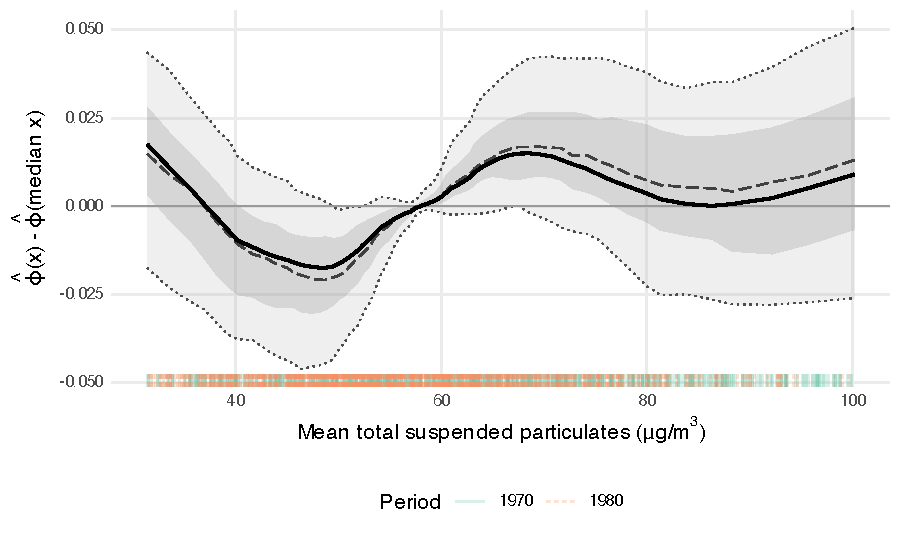
\includegraphics[width=0.92\textwidth]{../figures/app_tsp_phi.pdf}
\caption{The estimated hedonic price function and its variability}
\label{fig:app-phi}
\begin{minipage}{0.92\textwidth}\footnotesize
\textit{Notes:} $\hat\varphi(x)-\hat\varphi(x_{0.5})$ against mean total
suspended particulates, at $d_Z=5$, on the $983$-county Chay--Greenstone panel,
the instrument at its four trigger cells. Levels are log points of median
property value, normalised at the pooled median of $X$, $58.0\,\mu$g/m$^3$: the
figure carries shape, not level. The solid line is the point estimate and the
dashed line the median of $99$ bootstrap replications, which it tracks to within
$0.0049$ log points. The shaded regions are the twenty-fifth-to-seventy-fifth
and fifth-to-ninety-fifth percentiles of those replications, the outer dotted.
\emph{They illustrate variability and are not confidence sets; no coverage is
claimed for them and none is computed}, as in
\citet{centorrinofeveflorens2019}. The rug marks the marginal distribution of
$X$ in each period, thin in $1980$ above $80\,\mu$g/m$^3$ where few counties
support the curve. Source:
\texttt{scripts/application/app\_tsp\_02\_ladder.R} and
\texttt{app\_tsp\_05\_phi\_band.R}; figure
\texttt{paper/figures/app\_tsp\_phi.pdf}.
\end{minipage}
\end{figure}

\subsection{The bootstrap}\label{the-bootstrap}

Valid uniform inference on \(\hat\varphi\) does not exist in this model,
and the obstruction is a property of the estimator rather than of this
application. Uniform bands for ill-posed problems are built on a source
condition written in the spectral calculus of \(T^\ast T\) and on
completeness of the instrument, and neither is available here: the
operator equation of Section 2 is nonlinear in \(\varphi\), so there is
no adjoint in which to write the condition, and a \(W\) with four values
delivers completeness no more than a two-valued one does
\citep[see][]{severini2006,babiiflorens2025}. Pointwise sets do exist
under nonlinear ill-posedness \citep[see][]{chen2012b}, but they are
indexed by a sieve dimension where the regularisation index of
\cref{def:lfstep} is a Landweber iteration count. We therefore follow
the companion paper \citep{centorrinofeveflorens2019}, which estimates
the same operator equation from a discrete instrument under the same
regularisation: a point estimate, a bootstrap band drawn to show
variability, and one sentence saying what the band is not. \emph{The
envelope in \cref{fig:app-phi} illustrates the variability of
\(\hat\varphi\) and is not a confidence set. No coverage is claimed for
it and none is computed.}

The \(99\) replications resample counties with replacement and re-run
the regularisation in each, holding \(\hat\theta\) fixed, and the
envelope they give is wide against the curve it surrounds: its median
width over the sixty-point grid is \(1.33\) times everything the curve
does. Three further schemes ask whether that width is an artefact of the
resampling or a property of the estimator, since a resample of \(n\)
counties leaves roughly \(37\) per cent of the draw as duplicates while
halving the information: \(\mathrm{Exp}(1)\) multiplier weights, which
have the same first two moments and the same effective sample size but
duplicate nothing, and subsamples of \(621\) and of \(492\) distinct
counties. \emph{That comparison is not evaluable, and we report it as
such}: the three criteria that would have separated the two mechanisms
are all statements about the realised stopping index, and that index
equals the cap in every replication of every scheme, because the
discrepancy rule of Section 3 is run at \(\tau_{\mathrm{DP}}=0\) here
and the patience is set equal to the cap. What the schemes do show is
agreement on the size of the band, the multiplier arm being \(8.1\) per
cent narrower over the grid as a whole and wider at the ends of the
support. The five schemes are set out in Table S44 of the supplement,
the multiplier envelope in Table S45 of the supplement, and the eleven
levels this figure draws, together with the bootstrap's convergence
record, in Table S43 of the supplement.

\subsection{What the illustration
shows}\label{what-the-illustration-shows}

The estimator runs on this panel and returns the two objects it is built
to return: a slope vector with a clustered standard error, at either
cardinality of the instrument, and a structural curve whose shape
contradicts the constant slope the linear specification imposes. That is
the whole of what the section claims.

At \(n=983\) it claims nothing about the asymptotics, and there are two
reasons for that rather than one. Evaluated at \((\mu,r)=(2,\tfrac83)\),
the frontier-clearing configuration the Monte Carlo names, the frontier
\eqref{eq:frontier} is met at no control set that also satisfies A4(ii):
it fails once any control is entered, and the one rung at which it holds
is the intercept-only rung, which A4(ii) excludes because at
\(\alpha=\tfrac12\) the sieve-entropy condition admits no integer sieve
dimension (Table S49 of the supplement). The second is the cardinality
arm of the Monte Carlo, which finds the limit law's own remainder
failing to vanish at \(\mathsf L=4\) on the paper's named design (Table
S22 of the supplement), in a propensity direction whose price this panel
cannot bound because the N1 defect above is not resolvable from zero.
The object that describes this estimator at this sample size is
therefore \cref{cor:ratefloor} and not \cref{thm:rootn}. \emph{The
application illustrates the procedure on a design the method was built
for; it does not demonstrate that the asymptotics bind at this sample
size}, and we would rather say so than let the section be read as though
they did.

\section{Conclusions}\label{conclusions}

In this paper, we estimate the slope vector of a first-differenced
partially linear panel model whose nonparametric argument is a
continuous endogenous regressor and whose only instrument takes finitely
many values. Conditional independence between the differenced error and
the instrument replaces the conditional mean, a Bierens family converts
that restriction into unconditional moments, sieve Landweber--Fridman
regularisation solves the nonlinear equation that results, and a
cross-fitted one-step on a Neyman-orthogonal moment returns a slope
vector and a standard error.

Five results carry the paper.

Identification of \(\theta_\dagger\) runs through the mean restriction
alone and needs no source condition and no rank condition beyond
nonsingularity of \(E[\Delta Z\Delta Z']\). A moment free of the
structural function exists exactly when the two periods' tilted
marginals of the endogenous regressor coincide, so the partialling-out
route is closed here as a property of the differenced design and not of
the estimator. Orthogonality in the structural direction holds if and
only if the representer solves the adjoint equation, which is the range
condition of the linear theory read at a Fréchet derivative. Under A1
every set of instrument cells admits a common structural function, so a
conflict between two cells refutes A1 and attributes the refutation to
the cells that carry it, and that statement carries no identification
hypothesis at any subset of cells. And the cross-fitted one-step is
\(\sqrt n\)-consistent and asymptotically normal with a consistent
sample sandwich, whenever the first-stage rate is faster than
\(n^{-1/4}\).

What the extra cells buy is that attribution and nothing else. They do
not buy identification, a finer instrument making the identification
hypothesis weaker rather than stronger; they do not buy testability,
which is present already at \(\mathsf L=2\); and they do not buy
instrument strength, since splitting an instrument creates no variation.

Efficiency is not among them.

The sandwich is the variance the infeasible plug-in would carry at a
known \(\vdagger\), plus a positive semidefinite term that does not
vanish under overlap, and no semiparametric efficiency bound is computed
for this model. What the debiasing weight buys is the removal of a
first-order bias and not a smaller variance.

We assume two ingredients of the estimator to exist and construct
neither. The representer estimator \(\hat\ell\) is priced by A5(iv) at a
rate \(\epsilon_n\) with \(\delta_n\epsilon_n=o_P(n^{-1/2})\), and no
construction attaining it is supplied. The preliminary
\(\hat\varphi^{(0)}\) is needed at a declared deterministic envelope
\(\hat\varepsilon_0\) of polynomial order, for which consistency will
not do, and it has no supplier either. Three further conditions are
primitive rather than derived: \(\mu\) and \(\mathsf R_\ast\), global
identification of \(\vdagger\) at A1b(iii), and the sieve display of
Lemma L-7 on the sieve branch of the first-order bias.

The frontier is qualitative, and the Monte Carlo prices what that costs.
Crossing it makes the second-order remainder vanish eventually and says
nothing about where. At the configuration the theory names the turn
falls at \(n^{\ast}\approx10^{58}\), the simulated standard deviation
clears a two-standard-error bar only at \(n=181{,}019\) in DGP A and
only at the smaller of two equally admissible constants, and nominal
\(90\%\) intervals under-cover at \(29\) of the \(32\) cells; that
experiment is in the supplement, and Table S1 of the supplement carries
the standard-error units the sentence reads. What describes a panel
anyone will run is the rate floor of Section 4 and not the \(\sqrt n\)
statement. That reading is about the configuration and not about
\cref{thm:rootn}: at a design whose frontier margin is \(0.1318\) in
place of \(0.0060\), and whose propensity score is no smoother, the same
estimator meets the pre-committed coverage criterion from \(n=354\)
upward (Table S13 of the supplement) and clears the standard-deviation
ratio's two-standard-error bar from \(n=8{,}000\) at the same constant
(Table S19 of the supplement).

The stopping constant is the second open item. It is computable and not
identified, and at this configuration the criterion it thresholds falls
by \(11\) to \(43\) per cent over the whole iteration budget, so the
stop is settled almost entirely by a number the theory does not pin.
Whether a Lepskii-balanced rule should replace it turns on the
preliminary: given the discrepancy rule its own oracle constant, Lepskii
is ahead in all three cells started from zero and behind in all three
started from a rate-accurate one.

The third is severe ill-posedness, which the theorem does not reach.
Under exponentially decaying singular values the rate attainable from
any source condition is logarithmic, so the frontier fails at every
smoothness of the propensity score.

We run the estimator in Section 6 on the county panel of
\citet{chay2005}, where the object is the hedonic price of air quality
and the instrument is a nonattainment designation read as the pair of
triggers that produces it, at \(\mathsf L=4\). At \(n=983\) the frontier
fails at every control set an applied literature would accept (Table S49
of the supplement), so the object that describes the estimator there is
the rate floor and not \cref{thm:rootn}. That section illustrates the
procedure on a design the method was built for, and shows neither that
the asymptotics bind at this sample size nor anything about the Clean
Air Act. We take no position on A1 from it.

Future work should focus on constructing the two missing ingredients,
since a representer estimator with a rate and a preliminary with a
declared envelope would discharge the only maintained hypotheses that
name an object without building it. Recovering marginal effects from
\(\hat\varphi\) is a second step, and the derivative parameterisation is
not the route, since it lowers the source index below what the frontier
requires. A semiparametric efficiency bound for a model whose nuisance
solves an ill-posed nonlinear operator equation is a third, and a
statement uniform in \(P\) is a fourth. The latter would need a class on
which the \(P\)-specific constants are bounded, a uniform first-stage
rate at a random compressed operator, and a Lindeberg condition uniform
in \(P\).

Valid inference on \(\hat\varphi\) is a fifth, and Section 6 locates it.
Uniform bands in ill-posed models are built on a source condition
written at an adjoint and on completeness of the instrument, and a
nonlinear equation with a discrete instrument supplies neither
\citep[see][]{babii2016,severini2006,babiiflorens2025}.
\citet{chen2012b} do reach nonlinearly ill-posed conditional moment
models, but index their sets by a deterministic sieve dimension, while
the regularisation index of \cref{def:lfstep} is the random stopping
time of a discrepancy rule. The mathematics stops in the same place,
\citet{monardnicklpaternain2021} delivering Bernstein--von Mises for
nonlinear forward maps at smooth linear functionals only. Both
literatures give valid inference for the regular \(\sqrt n\) part and
neither goes past it, so \cref{thm:rootn} sits on that boundary rather
than short of it.

\section{Supplementary material}\label{supplementary-material}

Proofs of all results are in the online supplement. The supplement also
carries the statements this article refers to by name and does not
print, the interpretation of each numbered condition, and the smoothness
budget in one table. It repeats the statements printed here, in the same
order and under the same numbers, so that a proof and the result it
proves can be read together.

Two pointers appear in the statements above and both name a target in
the supplement rather than numbering one. \texttt{Lemma\ S:sandwich} is
the environment whose label is \texttt{lem:sandwich}, and
\texttt{(S:smdiff)} is the display whose label is \texttt{eq:smdiff}.
Each is the name the supplement gives the object, so it is findable
there by the heading it carries.

\clearpage
\small
\printbibliography


\printbibliography



\end{document}
